%%%%%%%%%%%%%%%%%%%%%%%%%%%%%%%%%%%%%%%%%%%%%%%%%%%%%%%%%%%%%%%
%% OXFORD THESIS TEMPLATE

% Use this template to produce a standard thesis that meets the Oxford University requirements for DPhil submission
%
% Originally by Keith A. Gillow (gillow@maths.ox.ac.uk), 1997
% Modified by Sam Evans (sam@samuelevansresearch.org), 2007
% Modified by John McManigle (john@oxfordechoes.com), 2015
% Modified by Ulrik Lyngs (ulrik.lyngs@cs.ox.ac.uk), 2018-, for use with R Markdown
%
% Ulrik Lyngs, 25 Nov 2018: Following John McManigle, broad permissions are granted to use, modify, and distribute this software
% as specified in the MIT License included in this distribution's LICENSE file.
%
% John commented this file extensively, so read through to see how to use the various options.  Remember that in LaTeX,
% any line starting with a % is NOT executed.  Several places below, you have a choice of which line to use
% out of multiple options (eg draft vs final, for PDF vs for binding, etc.)  When you pick one, add a % to the beginning of
% the lines you don't want.


%%%%% PAGE LAYOUT
% The most common choices should be below.  You can also do other things, like replacing "a4paper" with "letterpaper", etc.

% This one formats for two-sided binding (ie left and right pages have mirror margins; blank pages inserted where needed):
%\documentclass[a4paper,twoside]{templates/ociamthesis}
% This one formats for one-sided binding (ie left margin > right margin; no extra blank pages):
%\documentclass[a4paper]{ociamthesis}
% This one formats for PDF output (ie equal margins, no extra blank pages):
%\documentclass[a4paper,nobind]{templates/ociamthesis}

% As you can see from the uncommented line below, oxforddown template uses the a4paper size, 
% and passes in the binding option from the YAML header in index.Rmd:
\documentclass[a4paper, nobind]{templates/ociamthesis}


%%%%% ADDING LATEX PACKAGES
% add hyperref package with options from YAML %
\usepackage[pdfpagelabels]{hyperref}
% change the default coloring of links to something sensible
\usepackage{xcolor}

\definecolor{mylinkcolor}{RGB}{0,0,139}
\definecolor{myurlcolor}{RGB}{0,0,139}
\definecolor{mycitecolor}{RGB}{0,33,71}

\hypersetup{
  hidelinks,
  colorlinks,
  linktocpage=true,
  linkcolor=mylinkcolor,
  urlcolor=myurlcolor,
  citecolor=mycitecolor
}



% add float package to allow manual control of figure positioning %
\usepackage{float}

% enable strikethrough
\usepackage[normalem]{ulem}

% use soul package for correction highlighting
\usepackage{color, soul}
\definecolor{correctioncolor}{HTML}{CCCCFF}
\sethlcolor{correctioncolor}
\newcommand{\ctext}[3][RGB]{%
  \begingroup
  \definecolor{hlcolor}{#1}{#2}\sethlcolor{hlcolor}%
  \hl{#3}%
  \endgroup
}
\soulregister\ref7
\soulregister\cite7
\soulregister\autocite7
\soulregister\textcite7
\soulregister\pageref7

%%%%% FIXING / ADDING THINGS THAT'S SPECIAL TO R MARKDOWN'S USE OF LATEX TEMPLATES
% pandoc puts lists in 'tightlist' command when no space between bullet points in Rmd file,
% so we add this command to the template
\providecommand{\tightlist}{%
  \setlength{\itemsep}{0pt}\setlength{\parskip}{0pt}}
 
% UL 1 Dec 2018, fix to include code in shaded environments

% User-included things with header_includes or in_header will appear here
% kableExtra packages will appear here if you use library(kableExtra)
\usepackage{float}
\let\origfigure\figure
\let\endorigfigure\endfigure
\renewenvironment{figure}[1][2] {
    \expandafter\origfigure\expandafter[H]
} {
    \endorigfigure
}
\usepackage{booktabs}
\usepackage{longtable}
\usepackage{array}
\usepackage{multirow}
\usepackage{wrapfig}
\usepackage{float}
\usepackage{colortbl}
\usepackage{pdflscape}
\usepackage{tabu}
\usepackage{threeparttable}
\usepackage{threeparttablex}
\usepackage[normalem]{ulem}
\usepackage{makecell}
\usepackage{xcolor}


%UL set section header spacing
\usepackage{titlesec}
% 
\titlespacing\subsubsection{0pt}{24pt plus 4pt minus 2pt}{0pt plus 2pt minus 2pt}


%UL set whitespace around verbatim environments
\usepackage{etoolbox}
\makeatletter
\preto{\@verbatim}{\topsep=0pt \partopsep=0pt }
\makeatother



%%%%%%% PAGE HEADERS AND FOOTERS %%%%%%%%%
\usepackage{fancyhdr}
\setlength{\headheight}{15pt}
\fancyhf{} % clear the header and footers
\pagestyle{fancy}
\renewcommand{\chaptermark}[1]{\markboth{\thechapter. #1}{\thechapter. #1}}
\renewcommand{\sectionmark}[1]{\markright{\thesection. #1}} 
\renewcommand{\headrulewidth}{0pt}

\fancyhead[LO]{\emph{\leftmark}} 
\fancyhead[RE]{\emph{\rightmark}} 

% UL page number position 
\fancyfoot[C]{\emph{\thepage}} %regular pages
\fancypagestyle{plain}{\fancyhf{}\fancyfoot[C]{\emph{\thepage}}} %chapter pages

% JEM fix header on cleared pages for openright
\def\cleardoublepage{\clearpage\if@twoside \ifodd\c@page\else
   \hbox{}
   \fancyfoot[C]{}
   \newpage
   \if@twocolumn\hbox{}\newpage
   \fi
   \fancyhead[LO]{\emph{\leftmark}} 
   \fancyhead[RE]{\emph{\rightmark}} 
   \fi\fi}


%%%%% SELECT YOUR DRAFT OPTIONS
% This adds a "DRAFT" footer to every normal page.  (The first page of each chapter is not a "normal" page.)

% IP feb 2021: option to include line numbers in PDF

% This highlights (in blue) corrections marked with (for words) \mccorrect{blah} or (for whole
% paragraphs) \begin{mccorrection} . . . \end{mccorrection}.  This can be useful for sending a PDF of
% your corrected thesis to your examiners for review.  Turn it off, and the blue disappears.
\correctionstrue


%%%%% BIBLIOGRAPHY SETUP
% Note that your bibliography will require some tweaking depending on your department, preferred format, etc.
% If you've not used LaTeX before, I recommend reading a little about biblatex/biber and getting started with it.
% If you're already a LaTeX pro and are used to natbib or something, modify as necessary.
% Either way, you'll have to choose and configure an appropriate bibliography format...


\usepackage[style=numeric-comp, sorting=none, backend=biber, maxcitenames=2, useprefix, doi=true, isbn=false, uniquename=false]{biblatex}
\newcommand*{\bibtitle}{Works Cited}

\addbibresource{bibliography/references.bib}
\addbibresource{bibliography/additional-references.bib}


% This makes the bibliography left-aligned (not 'justified') and slightly smaller font.
\renewcommand*{\bibfont}{\raggedright\small}


% Uncomment this if you want equation numbers per section (2.3.12), instead of per chapter (2.18):
%\numberwithin{equation}{subsection}


%%%%% THESIS / TITLE PAGE INFORMATION
% Everybody needs to complete the following:
\title{Structural Analysis of Hemoprotein Binding Sites}
\author{Patrick Finnerty}
\college{Biosciences}

% Master's candidates who require the alternate title page (with candidate number and word count)
% must also un-comment and complete the following three lines:

% Uncomment the following line if your degree also includes exams (eg most masters):
%\renewcommand{\submittedtext}{Submitted in partial completion of the}
% Your full degree name.  (But remember that DPhils aren't "in" anything.  They're just DPhils.)
\degree{Master of Science}
% Term and year of submission, or date if your board requires (eg most masters)
\degreedate{Fall 2021}


%%%%% YOUR OWN PERSONAL MACROS
% This is a good place to dump your own LaTeX macros as they come up.

% To make text superscripts shortcuts
	\renewcommand{\th}{\textsuperscript{th}} % ex: I won 4\th place
	\newcommand{\nd}{\textsuperscript{nd}}
	\renewcommand{\st}{\textsuperscript{st}}
	\newcommand{\rd}{\textsuperscript{rd}}

%%%%% THE ACTUAL DOCUMENT STARTS HERE
\begin{document}

%%%%% CHOOSE YOUR LINE SPACING HERE
% This is the official option.  Use it for your submission copy and library copy:
\setlength{\textbaselineskip}{22pt plus2pt}
% This is closer spacing (about 1.5-spaced) that you might prefer for your personal copies:
%\setlength{\textbaselineskip}{18pt plus2pt minus1pt}

% You can set the spacing here for the roman-numbered pages (acknowledgements, table of contents, etc.)
\setlength{\frontmatterbaselineskip}{17pt plus1pt minus1pt}

% UL: You can set the line and paragraph spacing here for the separate abstract page to be handed in to Examination schools
\setlength{\abstractseparatelineskip}{13pt plus1pt minus1pt}
\setlength{\abstractseparateparskip}{0pt plus 1pt}

% UL: You can set the general paragraph spacing here - I've set it to 2pt (was 0) so
% it's less claustrophobic
\setlength{\parskip}{2pt plus 1pt}

%
% Oxford University logo on title page
%
\def\crest{{
\includegraphics[width=8cm]{templates/UABlogo.pdf}}}
\renewcommand{\university}{Universtat Autonoma de Barcelona}
\renewcommand{\submittedtext}{Academic Tutor, JeanDi, Dept of Chemistry; A thesis submitted for the degree of}


% Leave this line alone; it gets things started for the real document.
\setlength{\baselineskip}{\textbaselineskip}


%%%%% CHOOSE YOUR SECTION NUMBERING DEPTH HERE
% You have two choices.  First, how far down are sections numbered?  (Below that, they're named but
% don't get numbers.)  Second, what level of section appears in the table of contents?  These don't have
% to match: you can have numbered sections that don't show up in the ToC, or unnumbered sections that
% do.  Throughout, 0 = chapter; 1 = section; 2 = subsection; 3 = subsubsection, 4 = paragraph...

% The level that gets a number:
\setcounter{secnumdepth}{2}
% The level that shows up in the ToC:
\setcounter{tocdepth}{1}


%%%%% ABSTRACT SEPARATE
% This is used to create the separate, one-page abstract that you are required to hand into the Exam
% Schools.  You can comment it out to generate a PDF for printing or whatnot.

% JEM: Pages are roman numbered from here, though page numbers are invisible until ToC.  This is in
% keeping with most typesetting conventions.
\begin{romanpages}

% Title page is created here
\maketitle

%%%%% DEDICATION -- If you'd like one, un-comment the following.

%%%%% ACKNOWLEDGEMENTS -- Nothing to do here except comment out if you don't want it.
\begin{acknowledgements}
 	In case anyone reads this in the future, some context may be appreciated: I attended and completed this Master's during the COVID-19 global pandemic from September 2020 to September 2021.

  Thanks professors

  Thanks lab

  Thanks UAB

  Thanks Spain, and Catalonia, allowing me in and then also having public health measures unlike Donny's America

  Thanks classmates

  Thanks fam, friends

  Thanks to the media and the creators of media that facilitated the survival of my sanity through the pandemic.

  Finally, I'd like to quote a well-known artist from California. He was referencing his own work, but I wholly identify with his appreciation for the subject of his esteem:

  ``Last but not least, I wanna thank me. I wanna thank me for believing in me. I wanna thank me for doing all this hard work. I wanna thank me for having no days off. I wanna thank me for, for never quitting. I wanna thank me for always being a giver, and trying to give more than I receive. I wanna thank me for trying to do more right than wrong. I wanna thank me for just being me at all times.''
  -- Calvin Cordozar Broadus Jr.
\end{acknowledgements}


%%%%% ABSTRACT -- Nothing to do here except comment out if you don't want it.
\begin{abstract}
	Hemoproteins are able to catalyze an extraordinarily broad range of reactions. This class of proteins includes cytochrome P450s and peroxidases, among many others. Hemoproteins by definition include heme to achieve their chemistry; but heme molecules themselves vary considerably, and different heme molecules are employed depending on the function of the hemoprotein. At present, there is a knowledge gap in the literature of the structural features required to bind heme in hemoprotein binding sites.

 In this study, we investigated the binding environments of heme-b, heme-c, siroheme, and verdoheme. A high-throughput framework was developed to generate, process, and analyze data derived from the Protein Data Bank (PDB) files used in the study. Amino acid frequency, volume, surface areas, and angular relations within the heme binding sites were all examined for a diverse set of hemoproteins. Overall, we find that nonpolar residues and their interactions with heme may be of greater importance to heme binding than previously thought, suggesting that polar interactions, while necessary, are insufficient to efficiently bind heme. We also report several values for binding pocket volumes, surface areas, and angular data that may be of utility in artificial metalloenzyme design. The framework developed for this study is highly adaptable and may facilitate similar investigations for other proteins and ligands.
\end{abstract}

%%%%% MINI TABLES
% This lays the groundwork for per-chapter, mini tables of contents.  Comment the following line
% (and remove \minitoc from the chapter files) if you don't want this.  Un-comment either of the
% next two lines if you want a per-chapter list of figures or tables.
  \dominitoc % include a mini table of contents

% This aligns the bottom of the text of each page.  It generally makes things look better.
\flushbottom

% This is where the whole-document ToC appears:
\tableofcontents

\listoffigures
	\mtcaddchapter
  	% \mtcaddchapter is needed when adding a non-chapter (but chapter-like) entity to avoid confusing minitoc

% Uncomment to generate a list of tables:
\listoftables
  \mtcaddchapter
%%%%% LIST OF ABBREVIATIONS
% This example includes a list of abbreviations.  Look at text/abbreviations.tex to see how that file is
% formatted.  The template can handle any kind of list though, so this might be a good place for a
% glossary, etc.
% First parameter can be changed eg to "Glossary" or something.
% Second parameter is the max length of bold terms.
\begin{mclistof}{List of Abbreviations}{3.2cm}

\item[1-D, 2-D]

One- or two-dimensional, referring \textbf{in this thesis} to spatial dimensions in an image.

\item[Otter]

One of the finest of water mammals.

\item[Hedgehog]

Quite a nice prickly friend.

\end{mclistof} 


% The Roman pages, like the Roman Empire, must come to its inevitable close.
\end{romanpages}

%%%%% CHAPTERS
% Add or remove any chapters you'd like here, by file name (excluding '.tex'):
\flushbottom

% all your chapters and appendices will appear here
\hypertarget{lay-summary}{%
\chapter*{Lay Summary}\label{lay-summary}}
\addcontentsline{toc}{chapter}{Lay Summary}

\adjustmtc
\markboth{Lay Summary}{}

I investigated how heme, a molecule involved in many biological processes, binds to proteins. I did this by\ldots{}

\hypertarget{introduction}{%
\chapter*{Introduction}\label{introduction}}
\addcontentsline{toc}{chapter}{Introduction}

\adjustmtc
\markboth{Introduction}{}

Proteins that contain metal ion cofactor(s) are known as metalloproteins, and they compose approximately 40\% of all proteins. The metal ion can be free, or complexed with another molecule. One such molecule is heme, a complex of iron and a porphyrin ring. Heme is employed by many metalloproteins to catalyze a broad range of reactions.

There are many types of heme; but all of them are a coordination complex composed of an iron atom coordinated and bound to a modified porphyrin ring. Porphyins are composed of four pyrrole subunits (pentagonal structures of four carbons and a nitrogen) that are bound together via methine (i.e.~carbon) bridges (FIXME get a citation for this stuff). Porphyrins are considered macrocycles, molecules with large ring structures. The ring within porphyrins is heterocyclic, and considered aromatic, and therefore acts as a large resonant structure capable of transferring electrons. Coupled with an iron atom to enable reduction-oxidation reactions and the macrocycle of the porphyrin ring, the overall heme complex is therefore highly suited for reactions involving electron transfer.

Proteins containing heme are known as hemoproteins - hemoglobin and myoglobin are well-known examples, using heme to store and transport oxygen. Other examples of hemoproteins are peroxidases, catalases (a type of peroxidase), nitric oxide synthases, heme oxygenases, and cytochrome p450s. Peroxidases and catalases catalyze oxidation-reduction reactions using a histidine-bound heme, with catalases in particular specializing in the decomposition of hydrogen peroxide. Nitric oxide synthases catalyze the reaction of L-arginine into nitric oxide, which is vitally important to cellular signaling (\textcite{Poulos2014}). Free heme molecules may be released upon degradation of hemoproteins (especially hemoglobin), however, heme is prooxidative and therefore toxic to cells and must be cleared. Heme oxygenases assist in the degradation of heme, and are regarded as potential therapeutics, due to anti-inflammatory effects\autocite{Araujo2012}.

The enzymes with arguably the most potential applications, cytochrome P450s function as powerful monooxygenases. They participate in many reactions: capable oxidizing a wide range of substrates, including carbohydrates, steroids, fatty acids; catalyzing hormone degradation and synthesis; and degrading the majority of drugs(\textcite{Poulos2014}). Due to their extraordinary utility and range of reactions, cytochrome p450s are of great interest in the protein engineering field. Cytochrome P450s have the potential to be used in industrial biocatalysis, e.g.~in pharmaceutical production, bioremediation of environmental pollutants\autocite{Du2017,Lalonde2016}. The limiting factor preventing its deployment has been the struggle to increase enzymatic efficiency and therefore yield of processes employing the enzyme\autocite{Girvan2016,Li2020}.

Thus far, only heme-b and its respective hemoproteins have been discussed (although heme-b is the most abundant and most employed type of heme). Other types of heme are structurally and chemically different, and are used to achieve different chemical reactions. In this study, we examined heme-b, heme-c, verdoheme, and siroheme. Their structures are shown in Figures 1-5, and each heme is individually discussed below.

\#\#Types of Heme

\hypertarget{heme-b}{%
\subsection{Heme-b}\label{heme-b}}

\begin{figure}

{\centering 
\includegraphics[width=0.5\linewidth]{figures/HEM} 

}

\caption{Heme-b (HEM)}\label{fig:structHEM}
\end{figure}

The most common heme is heme-b. It is employed by the vast majority of hemoproteins. It is composed of an iron and porphyrin ring complex with attached vinyl and ethyl groups(FIXME?\ldots{} when we get the citation), and with the addition of two propionate groups. The iron atom is usually coordinated to a histidine or cysteine, depending on the enzyme.

The two propionate groups stabilize the heme in the pocket by forming polar interactions with salt bridges formed by arginine residues in the binding environment (Barrows). This behavior is the same for heme-b and likely verdoheme. It has also been suggested that the propionate groups may also serve to exclude solvent from the binding environment, potentially acting to expel and repel water molecules (Hayashi).

\hypertarget{heme-c}{%
\subsection{Heme-c}\label{heme-c}}

\begin{figure}

{\centering 
\includegraphics[width=0.5\linewidth]{figures/HEC} 

}

\caption{Heme-c (HEC)}\label{fig:structHEC}
\end{figure}

Heme-c is derived from heme-b. It is fairly similar to heme, with two notable differences: the iron atom binds, with few exceptions, covalently to cysteine residues in the binding pocket; and its two vinyl groups form thioester bonds with amino acids in the protein binding pocket. Its function is much more specific than heme-b, mostly serving as an electron carrier rather than catalyzing a plethora of reactions. The reason for this is not abundantly clear, but several studies suggest that because of its covalent bonding, heme-c has an electronic potential that is can be far lower and in general more broad, and more specifiable, than heme-b. \autocite{Bowman2008,Kleingardner2015}

\hypertarget{siroheme}{%
\subsection{Siroheme}\label{siroheme}}

\begin{figure}

{\centering 
\includegraphics[width=0.5\linewidth]{figures/SRM} 

}

\caption{Siroheme (SRM)}\label{fig:structSRM}
\end{figure}

Siroheme is even more limited in its applications, but highly specialized for its role. It is still an iron atom-porphyrin coordination complex, but it contains far more carboxyl and propionate groups than the other types of heme, making it highly polar. It is used exclusively in sulfite and nitrite reductases, which catalyze the reduction of the sulfates and nitrates plants uptake from the ground, providing the sources of nitrogen and sulfur used to produce nitrogen and sulfur-containing amino acids(\textcite{Tripathy2010}). The reason for the use of siroheme in this reaction rather than heme-b is not completely understood. But one study suggests that the bridge that siroheme forms between its catalyic iron atom, and the protein matrix environment (which also necessarily involves another cofactor, a cluster of cubane for electron transfer and provision) is more efficient at channeling electrons than the bridge that could be formed by heme.\autocite{Branzanic2019}

\hypertarget{verdoheme}{%
\subsection{Verdoheme}\label{verdoheme}}

\begin{figure}

{\centering 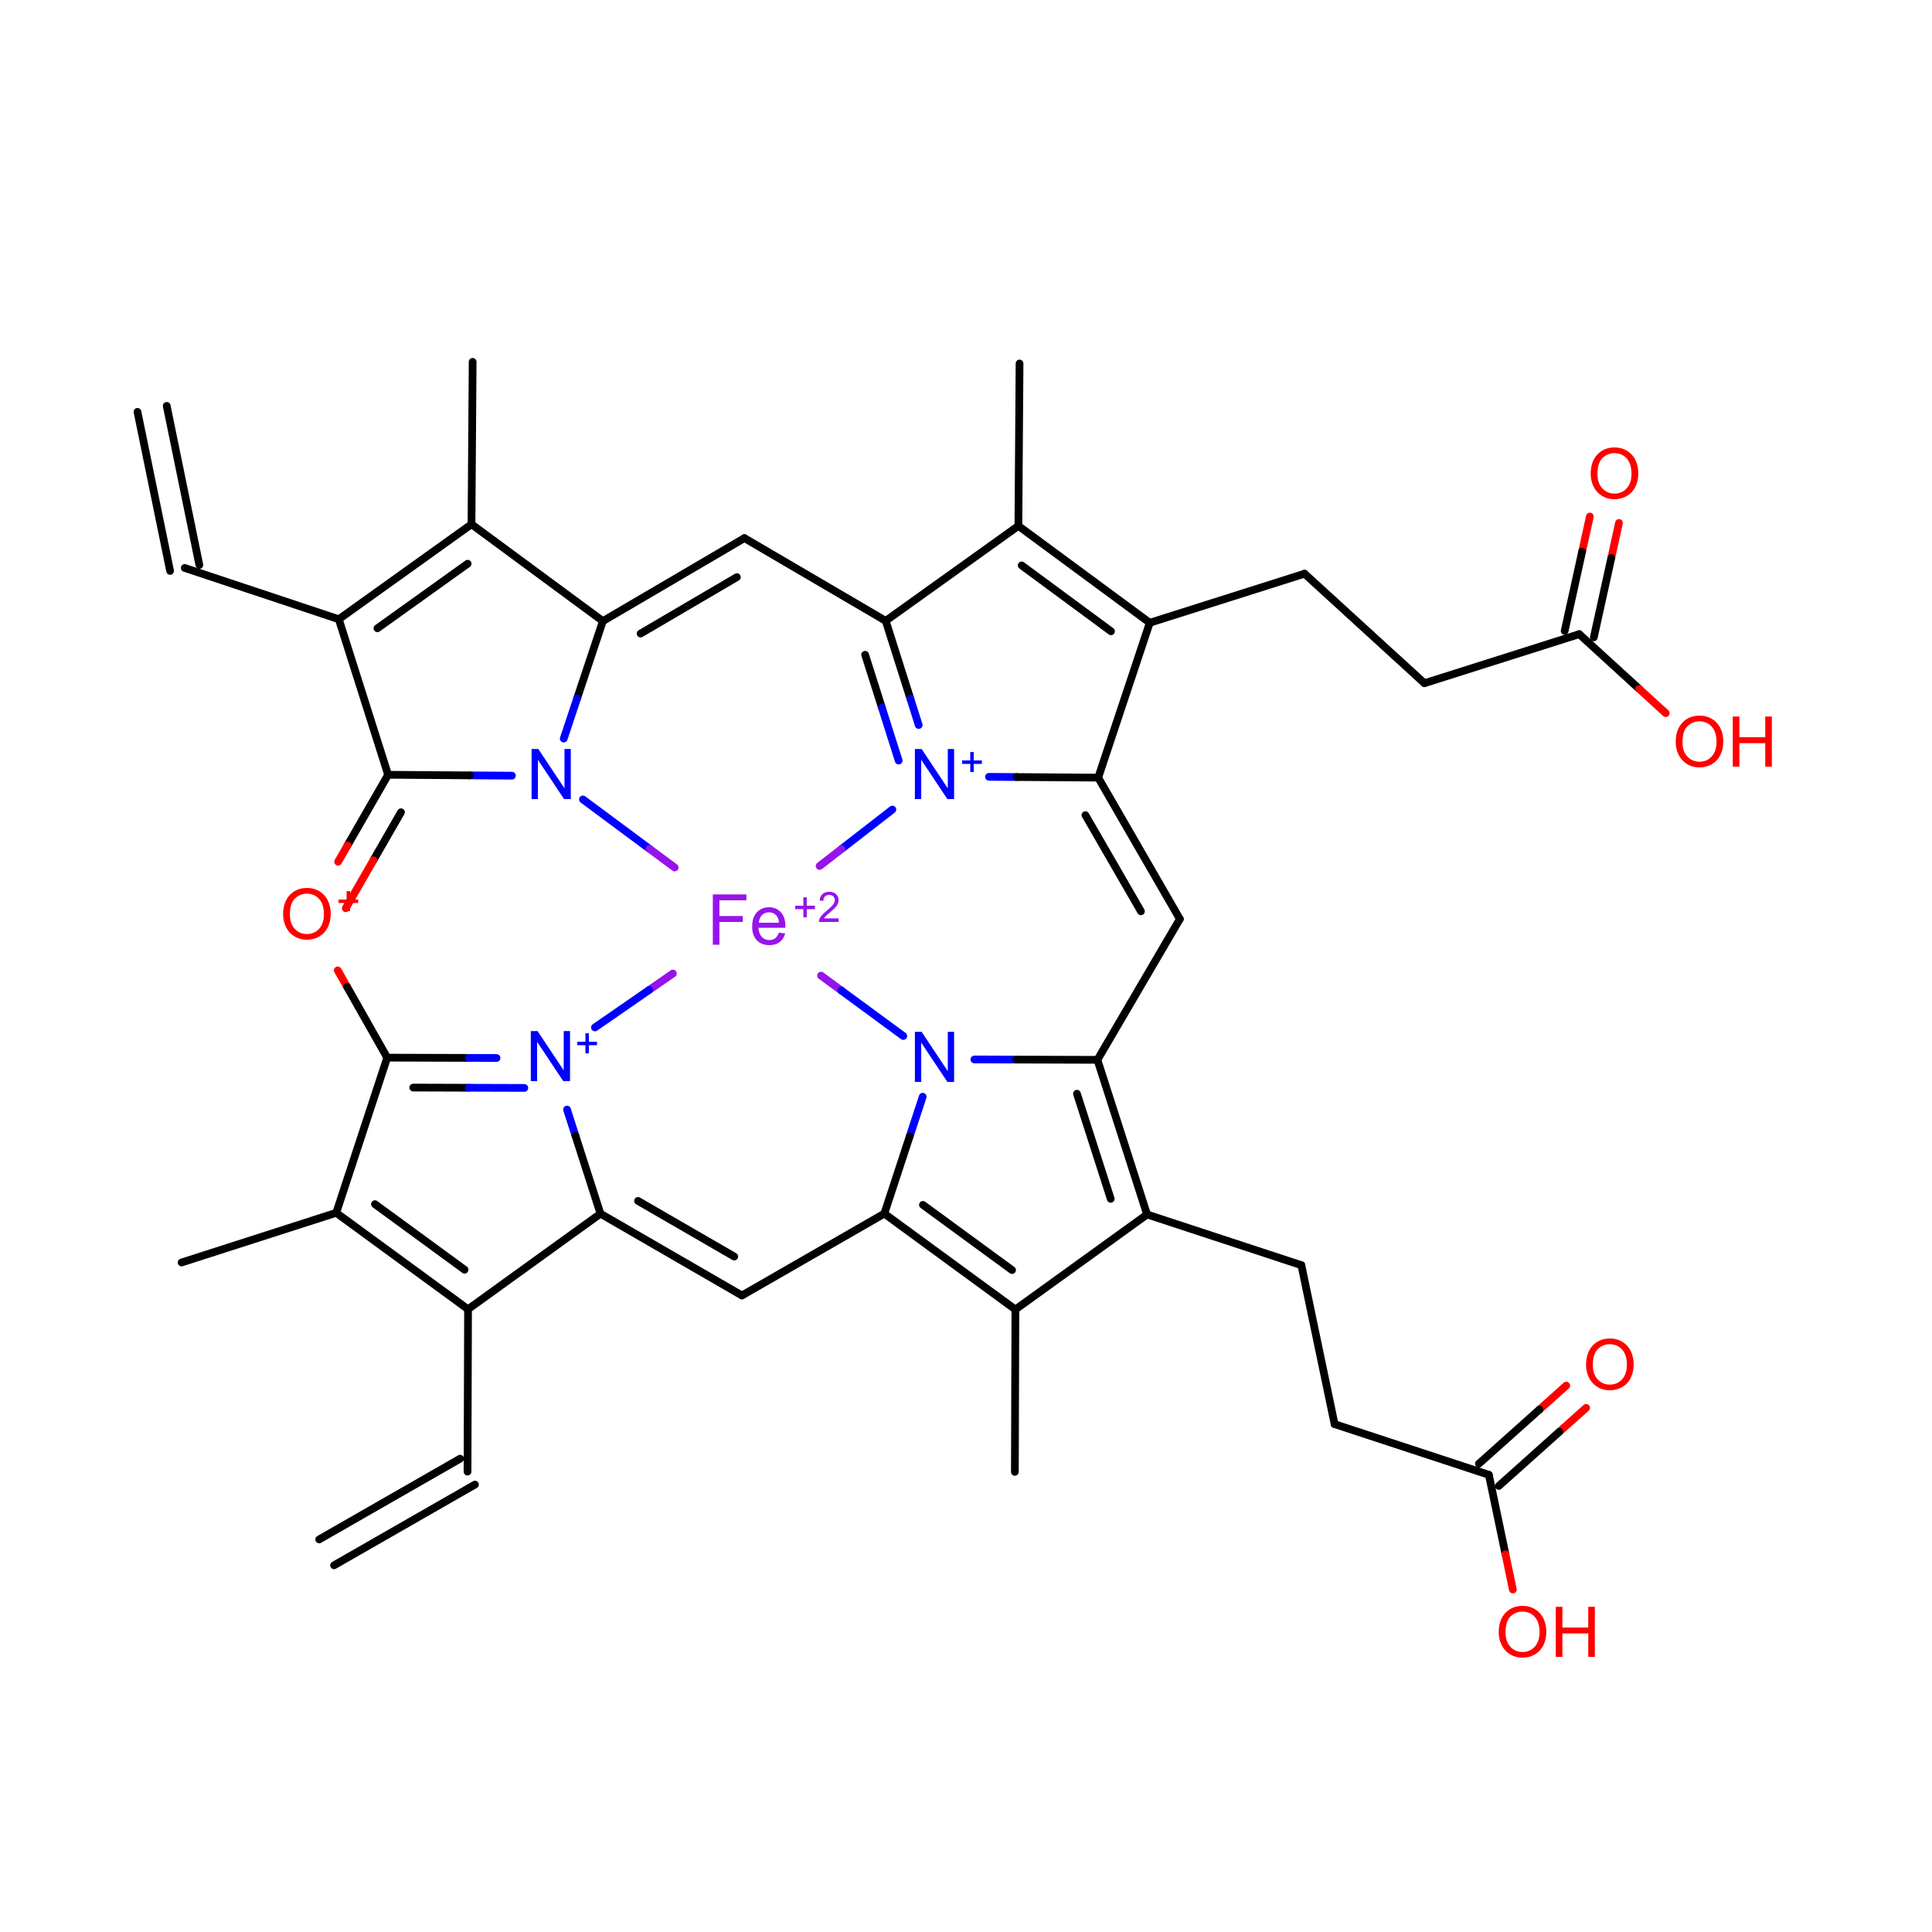
\includegraphics[width=0.5\linewidth]{figures/VEA} 

}

\caption{Verdoheme, VEA}\label{fig:structVEA}
\end{figure}
\begin{figure}

{\centering 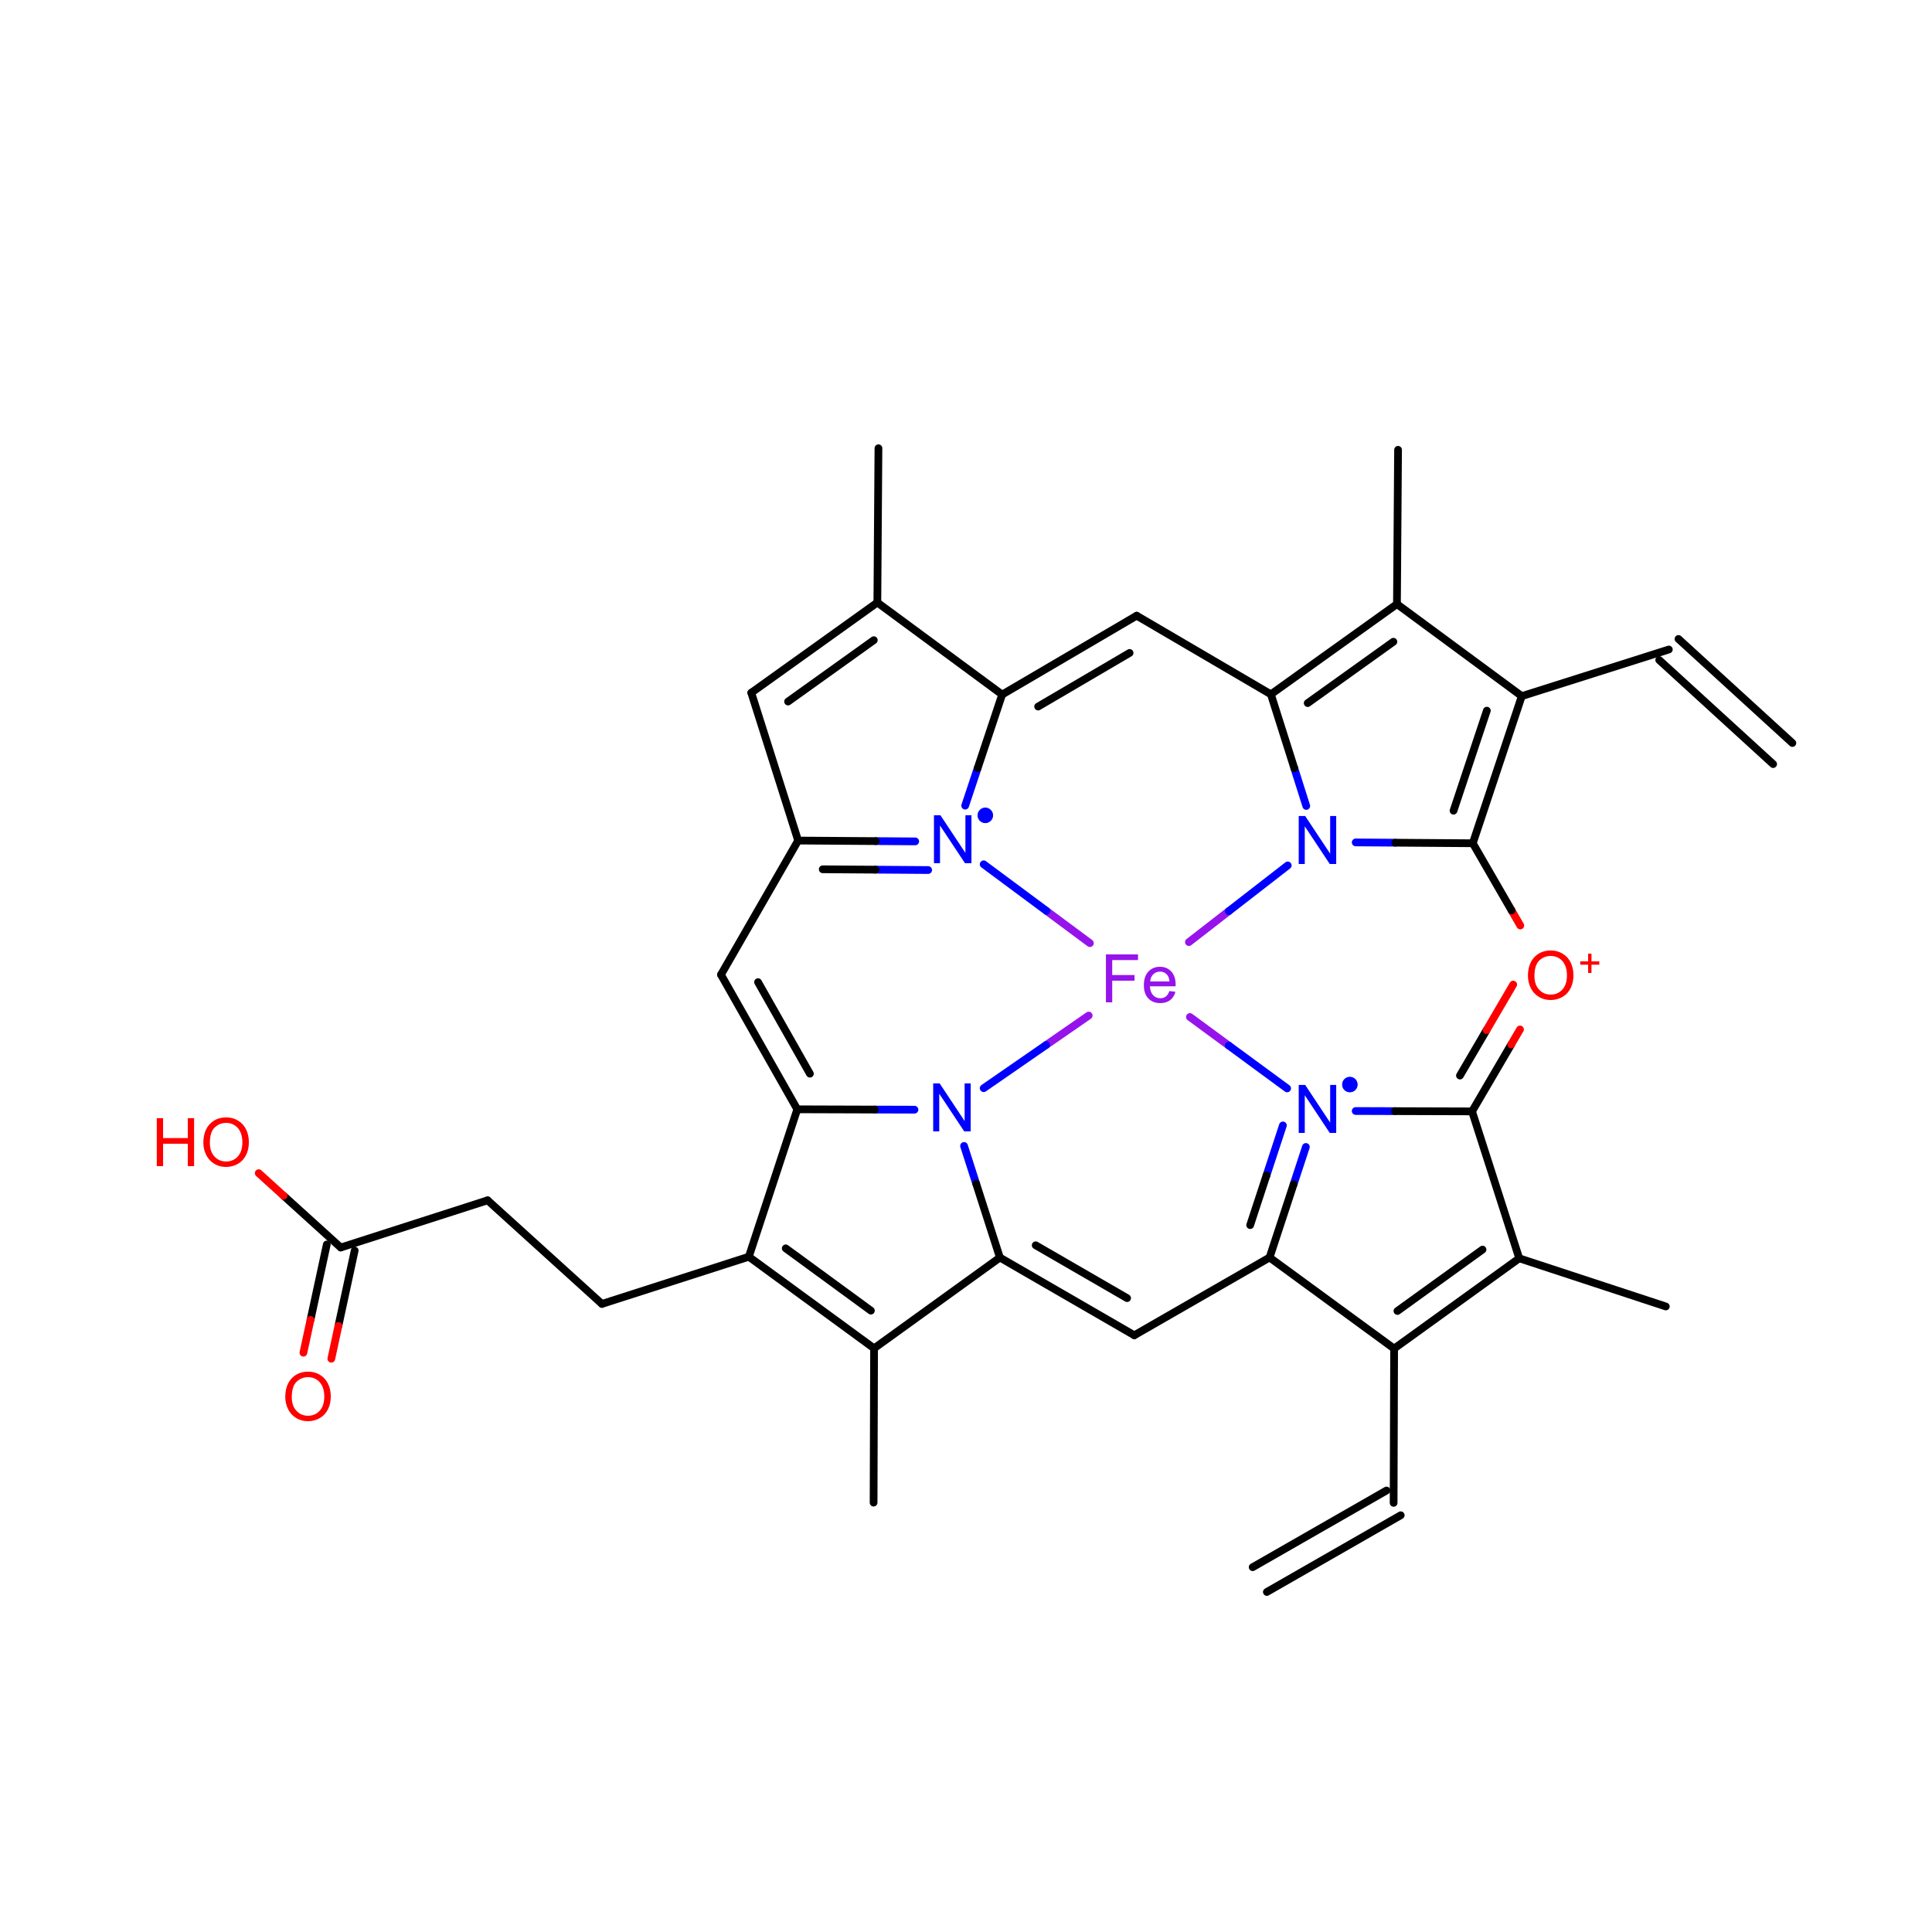
\includegraphics[width=0.5\linewidth]{figures/VER} 

}

\caption{Verdoheme, VER}\label{fig:structVER}
\end{figure}

Lastly, verdoheme is an intermediate product in the degradation of heme-b by heme oxygenase. When heme oxygenase degrades heme-b, biliverdin, carbon monoxide, and iron are produced; verdoheme is the precusor to bilverdin\autocite{Lai2010,Sato2007}. While a product of prior reactions wthin heme oxygenase, verdoheme appears to be oriented and bound differently \autocite{Lad2004}. The two structures used in the study, VEA and VER, are verdoheme at different stages of degradation, either partially oxidized or containing one less propionate group.

In summary, heme molecules can have very different structures and functions; they enable and catalyze an extraordinary amount, and extraordinarily diverse set of chemical reactions. They are important, not only as a study of how one class of molecule can be involved in a broad swath of reactions, but because hemoproteins have the potential to be of great value in biocatalysis, bioremediation, and pharmaceutical applications.

There is a significant barrier to the employment of hemoproteins in these areas, however: improving their efficiency far beyond what is found in nature. This is the field of artifical metalloproteins, or metalloenzymes: engineering metalloenzymes to improve them; increasing efficiency, stability, or even to introduce new reactions to heme's repetoire.

There are multiple methods employed to design these molecules, but rational design in particular (basically, the mutation of certain residues based on an understanding of the structure-function relationships) is at least partially hampered by an incomplete understanding of the binding environment for heme. For example, the importance of the binding environment was noted in a study seeking to design \emph{de novo} heme-c based enzymes, and found the binding environment likely to be of importance in modulating redox potential \autocite{Ishida2004}.

A fairly recent study conducted a structural analysis of 125 hemoprotein chains(\textcite{Li2011}). The study suggested hemoproteins undergo small conformational changes during binding; and that apo-form (ligand-containing) proteins may therefore be suitable for bioinformatics-based prediction and protein design. Additionally, the heme binding environments for both heme-b and heme-c were analyzed, and relative frequencies per amino acid were reported. Cysteine, histidine, phenylalanine, methionine, and tyrosine were found to be the most abundant residues within the binding environments of both heme-b and heme-c.~

The aforementioned study was published in 2011 - since then the PDB has been populated with far more hemoproteins. The focus of the study was on conformational differences induced by heme-binding, rather than the binding environment, although the relative frequencies of amino acids were reported. Interactions of the more abundant residues with heme-b or heme-c, including interactions with the porphyrin ring, were briefly discussed and this discussion will not be reproduced here.

In this study, we present research focused on elucidating the binding environment of multiple heme molecules: heme-b (HEM), heme-c (HEC), siroheme (SER), and verdoheme (VEA/VER). A diverse set of PDBs was assembled. UCSF Chimera was used to both extract and predict properties of a diverse set of hemoproteins. R was used to analyze the results. A robust and high-throughput framework was constructed to process the datasets for each heme molecule, requiring only inputs of which ligand was to be examined per dataset.

The properties extracted and predicted of the heme molecules' binding environments were: the amino acid frequencies; the distances of the amino acids from the heme iron; the volume of the binding pocket; and the surface areas of both the hemes and the binding pocket. These data can be expected to be of use, or at least of interest, to efforts in artifical metalloenzyme design.

Additionally, angular data for the residues within the binding environment were obtained. These data were produced more for exploratory purposes and are not discussed extensively in this study. Specifically, planar angles and the angle between residues' alpha-carbon, beta-carbon, and heme iron (CA-CB-Fe) were obtained.

These results may be of use in rational design of hemoproteins in future studies, or at least, improve the understanding of the heme binding environment.

\adjustmtc
\markboth{Methods}{}

\hypertarget{methods}{%
\chapter{Methods}\label{methods}}

\hypertarget{datasets}{%
\section{Datasets}\label{datasets}}

\noindent A list of PDBs was assembled that represented either a representative sample of a variety of proteins, with a resolution better than 3A, (HEM and HEC) or, all proteins containing these ligands were downloaded from the PDB (in the case of SRM, VER, VEA). Not all downloaded PDBs were appropriate for this study (e.g.~contained ``wobble'' structures) and therefore the amount of PDBs was culled. The datasets are current as of 16 August 2021.

The size of the datasets actually used in the study were as follows: HEM (n=58), HEC(n=13), SRM (n=9), VER (n=2) and VEA (n=2), which are merged for a combined n=4 for VERDOHEME.

The name of all proteins used in the study and their source organism are provided tables within Appendix \ref{molOrgSec}.

\hypertarget{preprocessing}{%
\section{Preprocessing}\label{preprocessing}}

Many of the PDBs downloaded were multimeric structures. The number of subunits per protein would skew results and overrepresent especially large multimeric proteins. Therefore, to only allow for one heme binding site per PDB, all downloaded PDBs were converted to monomeric structures. This was achieved by saving a single chain (chain A) of each PDB and eliminating all other chains. The single chain was then saved as a PDB and used in all subsequent scripts. Part of the script is reproduced below:

\textbf{INSERT SCRIPT, if we want}

\hypertarget{processing-monomers}{%
\section{Processing Monomers}\label{processing-monomers}}

UCSF-Chimera was used to generate all data in this study. Multiple Python scripts were employed to achieve a high-throughput process where all monomeric PDBs could be processed in the same session.

Chimera was used to predict the following qualities: Volume of the ligand binding pocket, accessible and excluded surface area of the ligand, and accessible and excluded surface area of the binding pocket. These calculations require a population of atoms to be selected for the calculation.

Atoms were selected within a distance cutoff, to be considered as ``interacting'' with the ligand or forming the binding pocket. Distance cutoffs from the ligand of 5A and 7A were chosen; for the predicted qualities, the algorithms were run twice to get values at 5A and 7A. For the distance and angle calculations, only the 7A distance cutoff was used, as the cutoff does not factor into any calculations and may be set during analysis.

As these cutoffs are selected arbitrarily, data from the 5A and 7A runs are overlaid in the figures reported in Appendix \ref{Figures}. Data tables are also provided in Appendix \ref{Tables}.

\hypertarget{amino-acid-frequency}{%
\subsection{Amino Acid Frequency}\label{amino-acid-frequency}}

Amino acids within the bounds of the lower and upper distance cutoff were selected and recorded. These were then counted for frequency per residue.

\hypertarget{volume-calculations}{%
\subsection{Volume Calculations}\label{volume-calculations}}

Volume of the binding pocket was predicted via Surfnet \autocite{Laskowski1995}, and run with default parameters of Grid Interval = 1.0 and Distance Cutoff = 10.0 (the latter option does not relate to the distance cutoff from the ligand). Surfnet is the molecular volume calculation tool implemented within UCSF Chimera. The script used selects the residues around heme to consider as the bounds of the pocket, but effectively ignores heme's presence as its calculates the volume, as if the pocket were empty:

Surfnet, at least in this investigation, was prone to generating very small volumes. During analysis these were removed and only the largest volume generated is recorded, since the largest volume generated and identified is most likely the binding pocket.

\textbf{insert code}

\hypertarget{surface-area-calculations}{%
\subsection{Surface Area Calculations}\label{surface-area-calculations}}

Solvent excluded and solvent accessible surface areas of both the ligand and the binding pocket were calculated using Chimera's ``surf'' algorithm, which itself is an implementation of a program called MSMS \autocite{Sanner1996}.

These two measures are similar but not the same. Solvent accessible surface area represents the surface area of the protein that a solvent molecule (i.e.~water) may interact with. It is calculated by rolling a sphere on the Van der Waals surface of the protein, and the \emph{center of the sphere} is recorded as the bounds of the accessible surface area. Solvent excluded surface area is calculated the same way, rolling a sphere on the Van der Waals surface of the protein, but instead the \emph{point of contact of the sphere against the Van der Waals surface} is recorded as the excluded surface area. The solvent excluded surface area may therefore be considered the bounds of the protein itself, versus the solvent accessible surface area, which can be considered the bounds at which a solvent may interact with the protein\autocite{Sanner1996}.

\hypertarget{distance-calculations}{%
\subsection{Distance Calculations}\label{distance-calculations}}

Distances of amino acids from the ligand could not be calculated accurately nor precisely in a direct way. Instead, distances for each atom composing a residue were calculated. This was achieved using a built-in function of chimera; the syntax is not straightforward, but part of the script is shown below. The distances of all atoms within a residue were averaged, and this value was taken as the mean distance of the entire residue and used in subsequent steps.

\textbf{insert some code}

The data produced in this step therefore include the mean distance of each amino acid. This is traceable, and the angular data below are cross-referenced with this list of distances. All data shown in figures (FIXME! Also for tables?) are multidimensional and may be filtered for distance.

\hypertarget{planar-angle-calculations}{%
\subsection{Planar Angle Calculations}\label{planar-angle-calculations}}

Individual residues and the ligand were defined as axes. The angle between each residue's axis and the axis of the ligand were calculated. Each axis functions essentially as a separate plane. (FIXME! Include a picture of what this looks like?) This employed the ``define axis'', and ``angle'' functions of Chimera; the Axes/Planes/Centroids Structural Analysis function of Chimera via GUI.

\hypertarget{ca-cb-fe-calculations}{%
\subsection{CA-CB-Fe Calculations}\label{ca-cb-fe-calculations}}

Residues within the distance cutoff were examined one by one. The angle of between each residue's carbon alpha (CA) and carbon beta (CB) and the Fe of the ligand was calculated, using the ``angle'' function of Chimera. The ligand nor the Fe atom were compared with themselves.

\hypertarget{import-to-r}{%
\section{Import to R}\label{import-to-r}}

The data produced by Chimera and the Python scripts were stored as .txt files. These files were imported to R and processed from text files into organized data formats. R was used to cross-reference angle and distance data. All plots and tables were constructed using R and imported directly to this document using Rmarkdown.

\adjustmtc
\markboth{Introduction}{}

\adjustmtc
\markboth{Methods}{}

\hypertarget{discussion}{%
\chapter{Results and Discussion}\label{discussion}}

\minitoc

--\textgreater{}

\hypertarget{analysis-of-residues-nearby-the-porphyrin-ring}{%
\section{Analysis of Residues Nearby the Porphyrin Ring}\label{analysis-of-residues-nearby-the-porphyrin-ring}}

We began the study by acquiring data to elucidate and quantify the propensity of amino acids to interact with heme (HEM, HEC, SRM, VEA/VER) in its binding environment. This study focused on potential interactions with the entire heme molecule, including the porphyrin ring and attached groups; therefore, any amino acids with potential interactons with the heme iron, porphyrin ring, or groups on the porphyrin ring (e.g.~vinyl, propionate groups), were included in the data gathered for this section. A potentially interacting amino acid was therefore defined as any amino acid with at least one atom within the distance cutoffs (5 and 7 Angstroms (A)) from the heme \emph{molecule}.

See Section \textbf{INSERT SECTION} in Methods to see how this looks within the script.

Amino acid frequencies were obtained for residues within the distance cutoffs of 5A and 7A - these figures and data are shown in \textbf{FIXME ADD APPENDICES LATER} The trends in these data are very similar and therefore only the data pertaining to the 7A distance cutoff are discussed below.

\hypertarget{disc-aaFreq}{%
\section{AA Frequency}\label{disc-aaFreq}}

\hypertarget{heme-b-1}{%
\subsection{Heme-b}\label{heme-b-1}}

\hypertarget{amino-acid-frequencies-in-binding-pocket}{%
\subsubsection{Amino Acid Frequencies in Binding Pocket}\label{amino-acid-frequencies-in-binding-pocket}}

Figure \ref{fig:HEM-AAfreq} plots the frequency of each residue within 7A of heme-b. Immediately below is Figure \ref{fig:HEM-AAfreqAll}, which plots the frequency of each residue within the entire monomer.

\begin{figure}
\centering
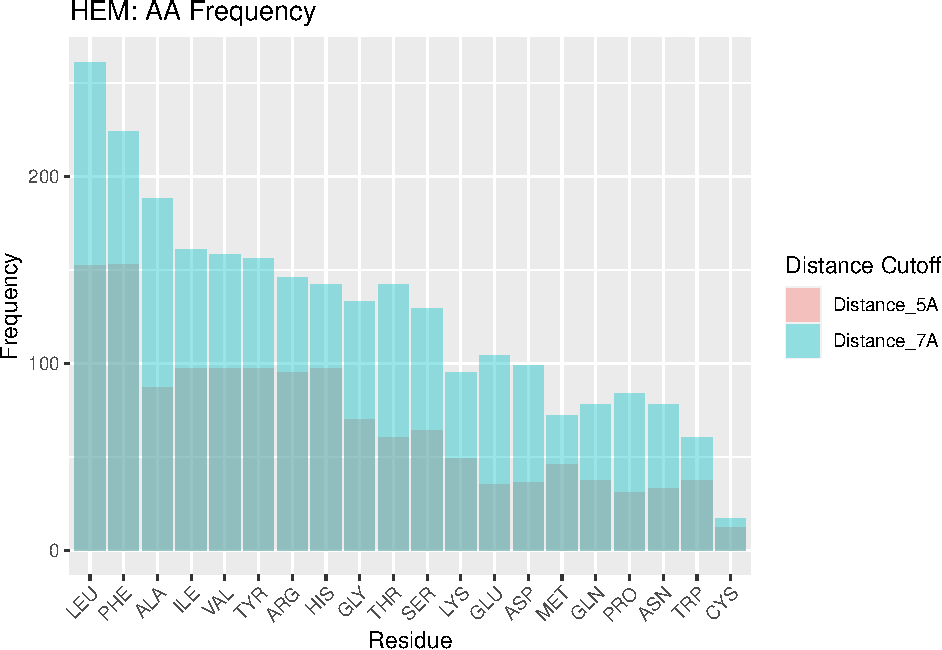
\includegraphics{_main_files/figure-latex/HEM-AAfreq-1.pdf}
\caption{\label{fig:HEM-AAfreq}HEM: AA Frequency within 7A}
\end{figure}

\begin{longtable}[t]{lr}
\caption{\label{tab:HEM-t-AAfreq}HEM AA Freq}\\
\toprule
Residue & Freq\\
\midrule
\endfirsthead
\caption[]{\label{tab:HEM-t-AAfreq}HEM AA Freq \textit{(continued)}}\\
\toprule
Residue & Freq\\
\midrule
\endhead

\endfoot
\bottomrule
\endlastfoot
\cellcolor{gray!6}{LEU} & \cellcolor{gray!6}{261}\\
PHE & 224\\
\cellcolor{gray!6}{ALA} & \cellcolor{gray!6}{188}\\
ILE & 161\\
\cellcolor{gray!6}{VAL} & \cellcolor{gray!6}{158}\\
\addlinespace
TYR & 156\\
\cellcolor{gray!6}{ARG} & \cellcolor{gray!6}{146}\\
HIS & 142\\
\cellcolor{gray!6}{THR} & \cellcolor{gray!6}{142}\\
GLY & 133\\
\addlinespace
\cellcolor{gray!6}{SER} & \cellcolor{gray!6}{129}\\
GLU & 104\\
\cellcolor{gray!6}{ASP} & \cellcolor{gray!6}{99}\\
LYS & 95\\
\cellcolor{gray!6}{PRO} & \cellcolor{gray!6}{84}\\
\addlinespace
ASN & 78\\
\cellcolor{gray!6}{GLN} & \cellcolor{gray!6}{78}\\
MET & 72\\
\cellcolor{gray!6}{TRP} & \cellcolor{gray!6}{60}\\
CYS & 17\\*
\end{longtable}

\textbf{I use `surprising, striking' a lot in this discussion. I'll reword this to have some variety later. The results are at least interesting!}

Beginning at the left of the figure and moving right, large, nonpolar amino acids appear most frequently within 7A: LEU and PHE; ILE appears less frequently than these two amino acids but nonetheless is in high frequency. Small, nonpolar amino acids ALA and VAL also appear very frequently. As the majority of the heme-b molecule is made up of the nonpolar porphyrin ring, these amino acids are therefore likely in such high frequency to provide the nonpolar interactions/environment with the pyrole groups and methyl and vinyl groups.

Tyrosine, arginine, histidine appear next most frequently. The two propionate groups on heme make polar interactions with salt bridges formed between arginine groups within the binding environment\autocite{Barrows2005}. Therefore, the tyrosine and histidine likely form polar interactions with the portion of the propionate groups not interacting with the arginine salt bridges. This, in addition to the nonpolar interactions above, likely provides as hospitable of a binding environment as possible to coordinate the heme. It should be noted histidine is one of the residues that coordinates the iron atom, and this may therefore increase its frequency in the binding pocket.

Glycine is a small residue and cannot form significant interactions within its environment; however, its frequency, or lack thereof (compared to background frequency, discussed later), suggests the binding pocket may not require as much flexibility or spatial considerations as in the rest of the protein. This would logically follow from the need for conserved binding sites.

Next appear serine, glutamate (glutamic acid) and aspartate (aspartic acid) and lysine. These are polar residues, and glutamate and aspartate are negatively charged; lysine is polar too, but positively charged. The negative charge is unlikely of importance in interaction with heme-b, however these polar amino acids likely again interact with the propionate groups on heme; only, infrequently. What is most interesting is why lysine is in such low abundance relative to the other polar, positively charged residues, arginine and histidine. Perhaps lysine's fairly linear structure prevents it from fitting into the binding pocket; however, arginine is also somewhat linear and features prominently, but this can be ascribed to its necessary formation and provision of salt bridges for polar interactions. The exact reason for why lysine would therefore be of low frequency could be is beyond the scope of this study.

Proline is a small nonpolar amino acid in low frequency; the trend for heme-b, at least, appears to be to favor large nonpolar amino acids in the binding pocket. This may suggest that a large amount of nonpolar interactions, per residue, is favored in the binding pocket, perhaps because of the limited space available to position residues to interact with heme.

Asparagine and glutamine are both medium-sized polar amino acids; given the trends already discussed it is surprising these are not in greater abundance. But as with proline, it may simply be a matter of maximizing the benefit of the interactions that may be formed with the heme; while asparagine and glutamine are polar, amino acids like arginine and histidine are both polar and positively charged (and arginine forms salt bridges), capable of stronger interactions with the electronegative propionate groups.

Methionine and tryptophan appear very infrequently in the binding pocket. Tryptophan is very surprising to find as second-to-least frequent. It is a large nonpolar amino acid - but perhaps its single, potential hydrogen bond, although weak, is enough to prefer completely nonpolar residues. Or, with its size, it is preferable to have more numerous, smaller nonpolar residues that can favorably interact with the porphyrin while reducing steric hindrance of other residues in the environment (taking up less space). The reason for methionine's low frequency is not clear, perhaps for similar reasons as with proline, where more nonpolar residues are preferred, rather than less nonpolar residues being unfavorable.

Cystine appears most infrequently of all the amino acids in the binding pocket. This is quite surprising - cystine is highly evolutionarily conserved to coordinate the iron in the binding pocket. Perhaps the sample of PDBs used in this study mostly use histidine to coordinate the iron - but this would only account for one residue in the binding pocket per pdb. Therefore these results suggest that while cystidine may be well suited to coordinate the iron in heme, it is poorly suited to form any nonpolar interactions with the porphyrin ring, leaving the task up to other, more suitably, intensely nonpolar amino acids.

Moving away from discussing individual amino acid populations, what is especially notable of the data for heme-b is that nonpolar residues appear in much greater frequency than polar residues. Nonpolar interactions with heme are therefore more numerous than polar interactions; quite logical, given there are only two polar propionate groups on a large porphyrin ring that is otherwise nonpolar. Their multiplicity may also suggest that they are potentially of greater importance than previously thought. At the very least, these results suggest that polar interactions and coordination of the iron atom, while necessary for heme binding, are insufficient, and that nonpolar intercations and the population of nopolar residues in the binding pocket should be considered when examining the binding environment of heme.

\hypertarget{comparison-with-background-amino-acid-frequencies}{%
\subsubsection{Comparison with Background Amino Acid Frequencies}\label{comparison-with-background-amino-acid-frequencies}}

While the frequencies of amino acids in the binding pocket have been discussed, it may also be of interest to compare against the background amino acid frequency, the general frequency of amino acids within the entire monomer. The degree to which this may affect the significance of the frequencies of the amino acids in the binding pocket is unclear - those amino acids are still employed and placed such as to bind the heme, rather than being a random assortment of residues. However, an in depth examination of simlarities and differences may reveal that some amino acids may simply be extremely highly conserved by chance and by virtue of their numerous population, rather than some chemical benefit.

Figure \ref{HEM-AAfreqAll} documents the frequencies of amino acids overall within the monomer.

Leucine and alanine as in the binding pocket frequencies are highly frequent in the overall monomer. This may suggest their prevalence in the binding pocket may simply be due to a high population of leucine and alanine in hemoproteins.

However, after these two amino acids the tendencies in frequency for the binding pocket and the monomer at large diverge.
Glycine is in high frequency - likely due to more complex geometry e.g.~helices outside the binding pocket. In interest of brevity, the remaining frequencies are summed up thus: the same trends that appear to exist in the binding pocket do not appear to exist in the monomer at large. While the order of frequencies in conserved binding pockets can be rationalized, justifying the overall frequencies in monomers invites significant speculation.

\begin{figure}
\centering
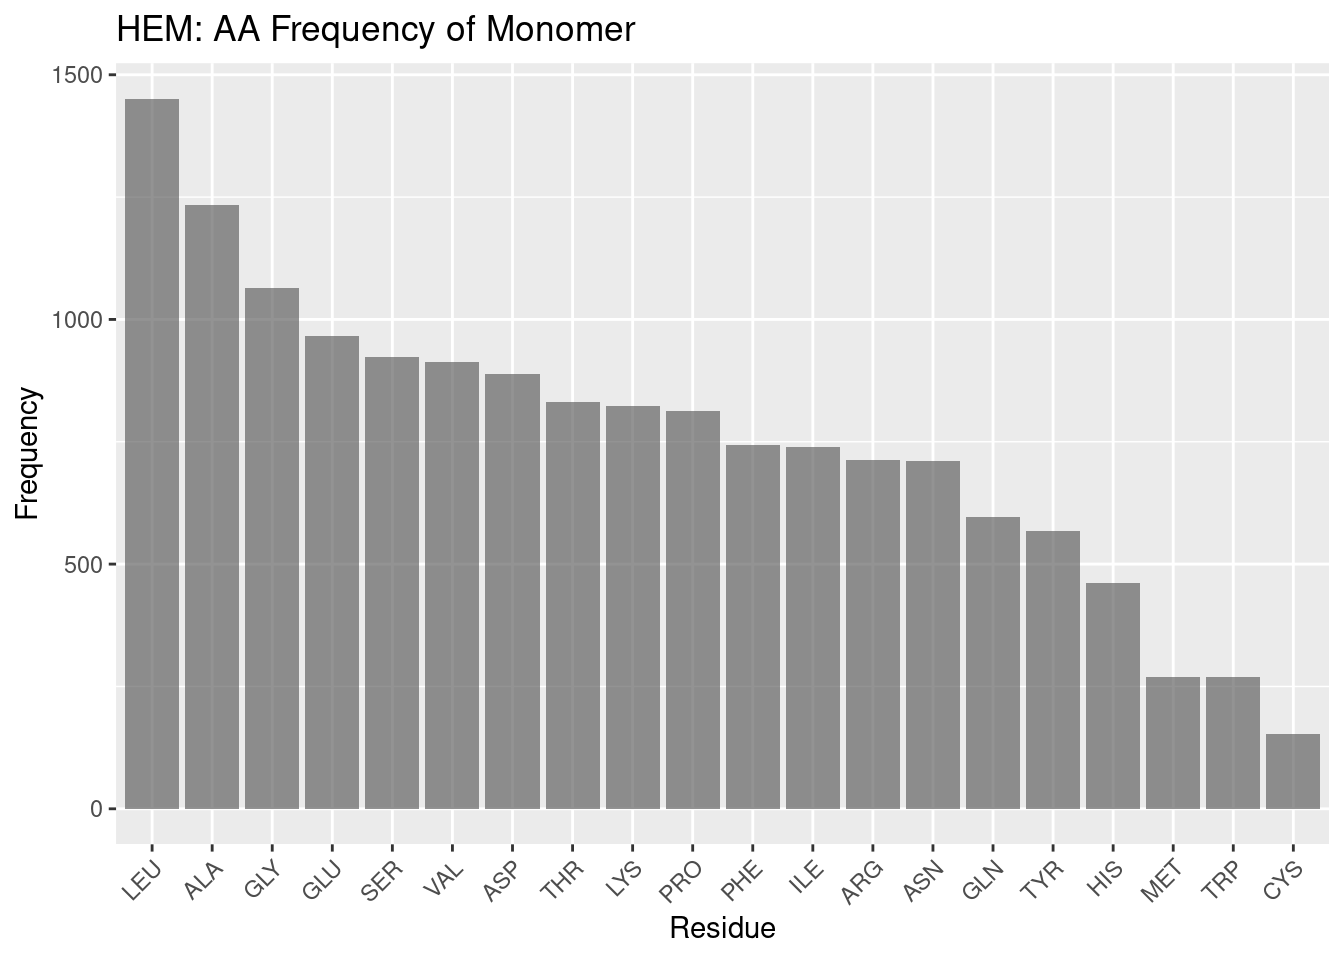
\includegraphics{_main_files/figure-latex/HEM-AAfreqAll-1.pdf}
\caption{\label{fig:HEM-AAfreqAll}HEM: AA Frequency of Monomer}
\end{figure}

\hypertarget{distributon-of-amino-acids-over-distance}{%
\subsubsection{Distributon of Amino Acids over Distance}\label{distributon-of-amino-acids-over-distance}}

After an exhaustive exploration of the relative frequencies of amino acids in the binding pocket, the figure below is fairly straightfoward. Figure \ref{fig:HEM-AAdist} plots the distribution of amino acids in the binding pocket against their distance from the iron of the heme.

We find that only a few residues come in close contact (\textless4A) of the heme: Cys, His, Tyr. Most residues center their distribution at around 6A, although Lys seems more biased than the remaining residues to be a bit closer. Cysteine and histidine may be at least in part explained to be close due to their use as coordinating residues; histidine, being in greater frequency, may also be this close due to favorable interactions with the porphyrin ring.

The proximity of tyrosine however, is more notable. It cannot form coordination bonds with the heme iron, but tyrosine residues do interact with the propionate groups. Tyrosine is also required for redox reactions, and part of the population of tyrosine residues may therefore be in close proximity to heme to facilitate electron transfer in various enzymes\autocite{Poulos2014}. These results suggest that of all potentially interacting polar/positively charged residues, tyrosine is the most likely at least to be in close proximity to the heme molecule. Whether this illustrates an extreme importance of tyrosine to interact with propionate groups, or instead the need for tyrosine to be in close proximity in order to form such interactions, or simply demonstrates coordination of oxidation/reduction reactions, is beyond the scope of this study.

\begin{figure}
\centering
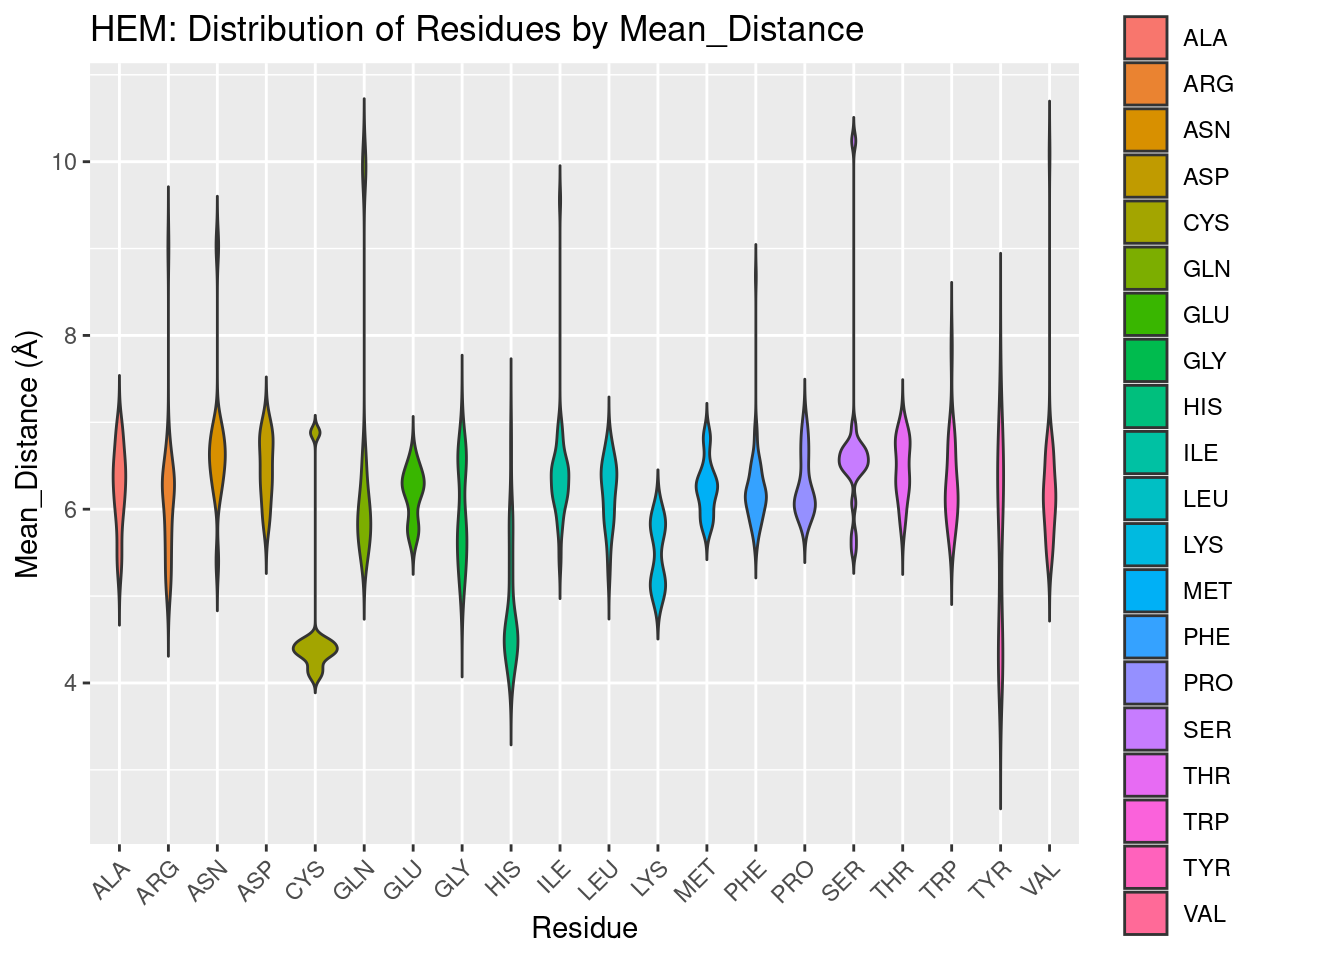
\includegraphics{_main_files/figure-latex/HEM-AAdist-1.pdf}
\caption{\label{fig:HEM-AAdist}HEM: AA Distances}
\end{figure}

\hypertarget{heme-c-1}{%
\subsection{Heme-c}\label{heme-c-1}}

\begin{figure}
\centering
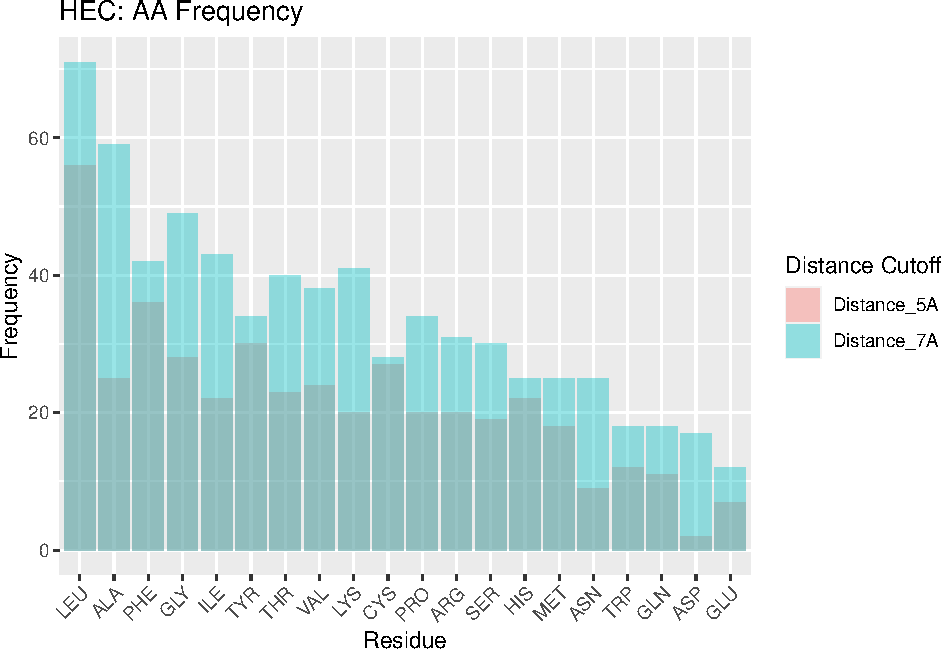
\includegraphics{_main_files/figure-latex/HEC-AAfreq-1.pdf}
\caption{\label{fig:HEC-AAfreq}HEC: AA Frequency}
\end{figure}

\begin{longtable}[t]{lr}
\caption{\label{tab:HEC-t-AAfreq}HEC AA Freq}\\
\toprule
Residue & Freq\\
\midrule
\endfirsthead
\caption[]{\label{tab:HEC-t-AAfreq}HEC AA Freq \textit{(continued)}}\\
\toprule
Residue & Freq\\
\midrule
\endhead

\endfoot
\bottomrule
\endlastfoot
\cellcolor{gray!6}{LEU} & \cellcolor{gray!6}{62}\\
ALA & 47\\
\cellcolor{gray!6}{GLY} & \cellcolor{gray!6}{39}\\
LYS & 38\\
\cellcolor{gray!6}{PHE} & \cellcolor{gray!6}{35}\\
\addlinespace
VAL & 35\\
\cellcolor{gray!6}{ILE} & \cellcolor{gray!6}{34}\\
THR & 34\\
\cellcolor{gray!6}{TYR} & \cellcolor{gray!6}{30}\\
ARG & 26\\
\addlinespace
\cellcolor{gray!6}{PRO} & \cellcolor{gray!6}{26}\\
CYS & 24\\
\cellcolor{gray!6}{MET} & \cellcolor{gray!6}{23}\\
HIS & 21\\
\cellcolor{gray!6}{SER} & \cellcolor{gray!6}{21}\\
\addlinespace
ASN & 20\\
\cellcolor{gray!6}{GLN} & \cellcolor{gray!6}{17}\\
ASP & 14\\
\cellcolor{gray!6}{TRP} & \cellcolor{gray!6}{12}\\
GLU & 11\\*
\end{longtable}

Leucine and alanine again are highly frequent for HEC, followed by quite similar trends, and therefore HEC will not be as thoroughly discussed as HEM. The most notable differences may be that GLY and CYS are in far higher frequency than in heme. Heme-c almost always forms covalent bonds with cysteine residues, and this may explain that frequency. But as for the high frequency of glycine, the reason for its abundance is unclear, although it seems it has an important role in heme-c pockets.

\hypertarget{comparison-to-background-frequency}{%
\subsubsection{Comparison to background frequency}\label{comparison-to-background-frequency}}

\begin{figure}
\centering
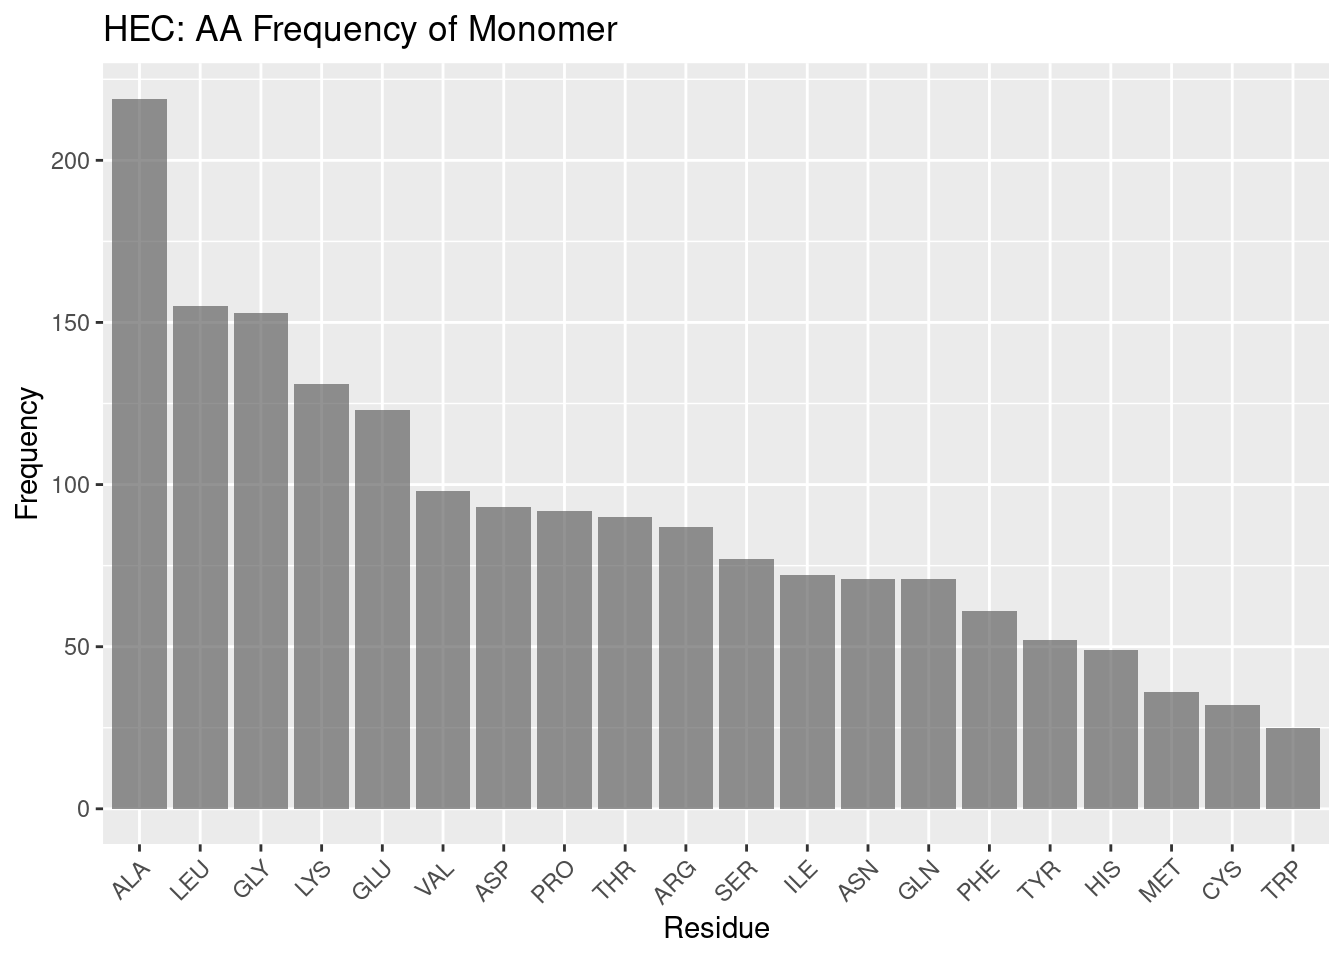
\includegraphics{_main_files/figure-latex/HEC-AAfreqAll-1.pdf}
\caption{\label{fig:HEC-AAfreqAll}HEC: AA Frequency of Monomer}
\end{figure}

Generally, the heme-c monomer is similar to the heme-b monomer, with a high frequency of alanine and leucine, followed by a divergence in the frequency of amino acids and therefore a struggle to form any meaningful discussion when it comes to comparing the binding pocket frequencies against background frequencies.

\hypertarget{aa-distribution-v.-distance}{%
\subsubsection{AA Distribution v. Distance}\label{aa-distribution-v.-distance}}

\begin{figure}
\centering
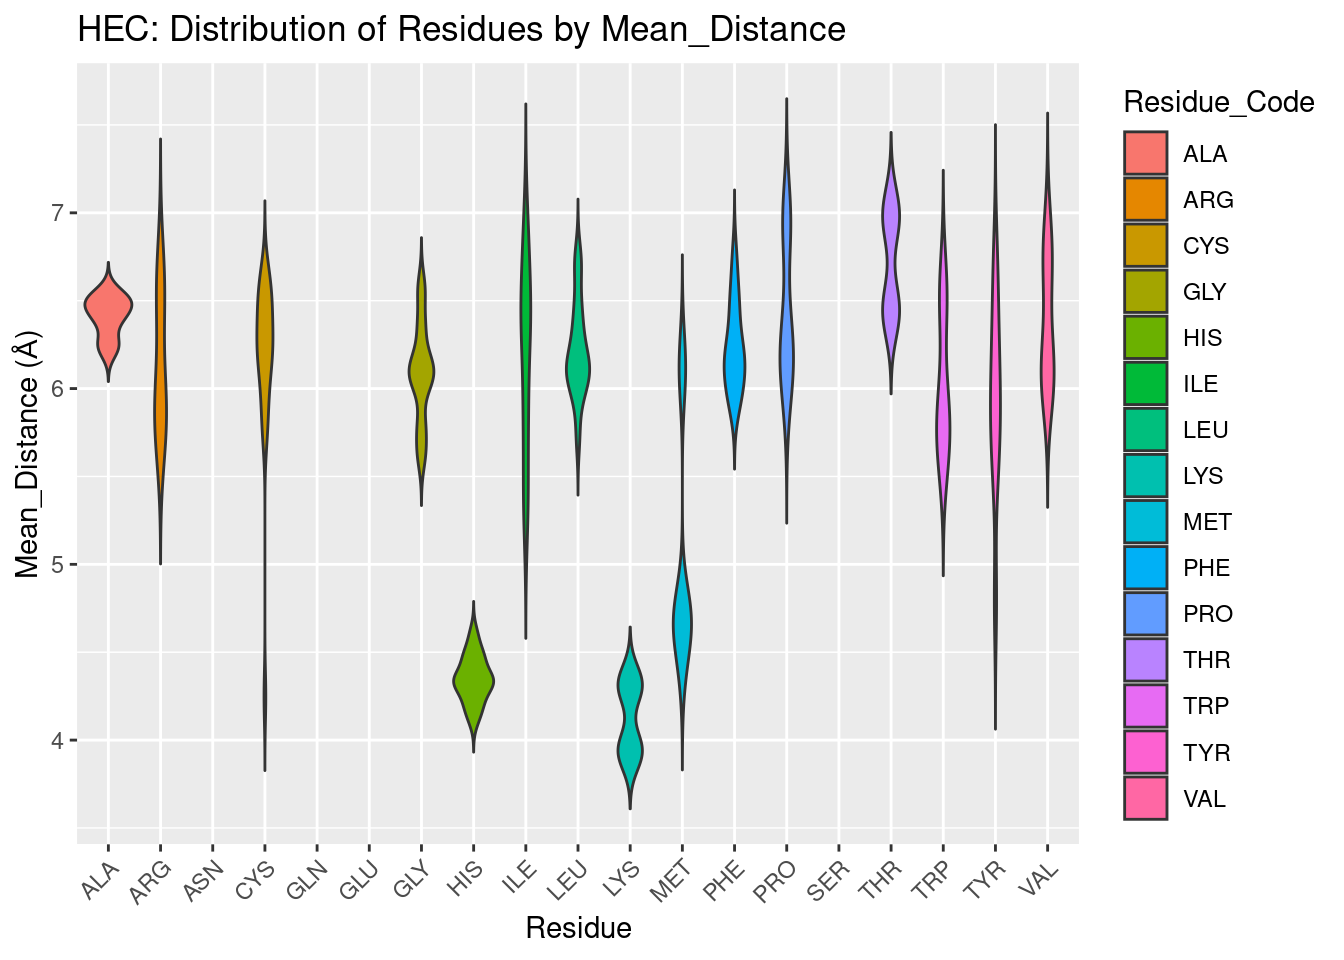
\includegraphics{_main_files/figure-latex/HEC-AAdist-1.pdf}
\caption{\label{fig:HEC-AAdist}HEC: AA Distances}
\end{figure}

The distribution of amino acids over distance from the heme iron for HEC is similar to HEM, with some exceptions. Cys, His, Tyr again are amongst the closest residues to HEC, likely for the same reasons of very strong polar interactions or coordination. Additionally, cysteine forms covalent, thioester bonds with heme-c, providing further justification for its proximity. However, for heme-c, lysine and methionine also are very proximal. The methionine residues are nonpolar, small, neutral; lysine is polar and positively charged; neither of these residues are favored to be included in the heme-b binding environment despite very similar structures. The reason for their inclusion so close to the binding pocket is therefore unclear, but based on their distribution, and lysine being even more close proximity than heme, the results suggest these two residues may have important roles.

\hypertarget{verdoheme-1}{%
\subsection{Verdoheme}\label{verdoheme-1}}

\begin{figure}
\centering
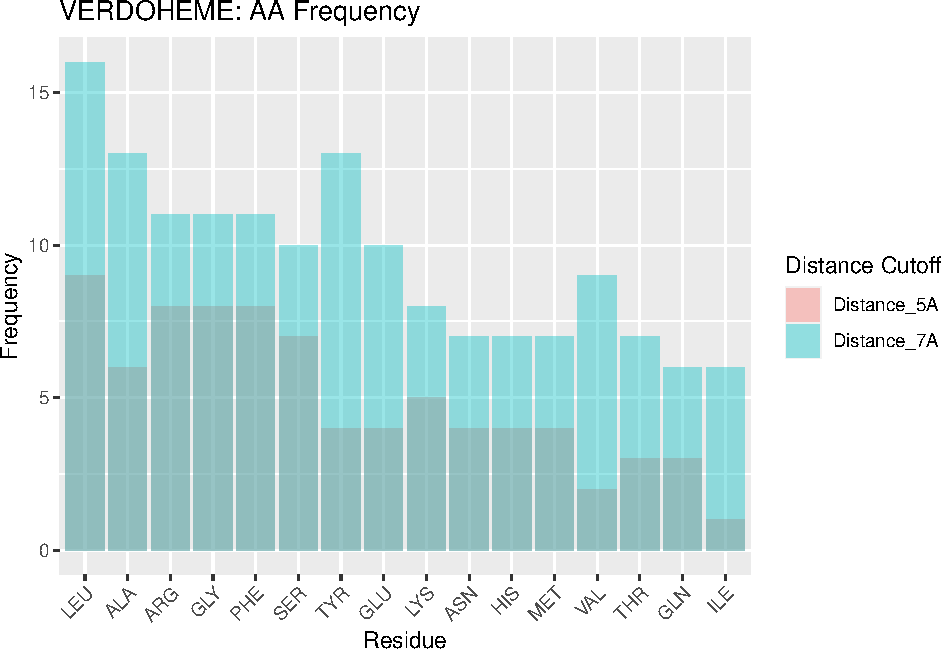
\includegraphics{_main_files/figure-latex/VERDOHEME-AAfreq-1.pdf}
\caption{\label{fig:VERDOHEME-AAfreq}VERDOHEME: AA Frequency}
\end{figure}

\begin{longtable}[t]{lr}
\caption{\label{tab:VERDOHEME-t-AAfreq}VERDOHEME AA Freq}\\
\toprule
Residue & Freq\\
\midrule
\endfirsthead
\caption[]{\label{tab:VERDOHEME-t-AAfreq}VERDOHEME AA Freq \textit{(continued)}}\\
\toprule
Residue & Freq\\
\midrule
\endhead

\endfoot
\bottomrule
\endlastfoot
\cellcolor{gray!6}{LEU} & \cellcolor{gray!6}{16}\\
ALA & 13\\
\cellcolor{gray!6}{TYR} & \cellcolor{gray!6}{13}\\
ARG & 11\\
\cellcolor{gray!6}{GLY} & \cellcolor{gray!6}{11}\\
\addlinespace
PHE & 11\\
\cellcolor{gray!6}{GLU} & \cellcolor{gray!6}{10}\\
SER & 10\\
\cellcolor{gray!6}{VAL} & \cellcolor{gray!6}{9}\\
LYS & 8\\
\addlinespace
\cellcolor{gray!6}{ASN} & \cellcolor{gray!6}{7}\\
HIS & 7\\
\cellcolor{gray!6}{MET} & \cellcolor{gray!6}{7}\\
THR & 7\\
\cellcolor{gray!6}{GLN} & \cellcolor{gray!6}{6}\\
\addlinespace
ILE & 6\\
\cellcolor{gray!6}{ASP} & \cellcolor{gray!6}{4}\\*
\end{longtable}

Verdoheme is dissimilar from HEM and HEC above. This is fairly surprising, given that verdoheme is an intermediate in the binding pocket for heme within heme oxygenases. The results discussed below may be attributable to the small sample size of verdoheme PDBs (n=4, combining VEA and VER), and should be appreciated with some skepticism. Nonetheless, the results will be discussed.

Leucine and alanine are again most frequent, but after these, results diverge. Tyrosine and arginine are next most frequent - surprising, given that this is still the same pocket that bound heme. The data for heme-b indicate more frequent nonpolar residues before tyrosine. Chemically, it may be that as heme is oxidized, there is greater need for polar interactions; this would help to explain the high frequency of polar residues, but does not explain the shift in amino acid frequencies within what should be a similar binding pocket - all verdoheme PDBs in this in study were sourced from heme oxgenase proteins. Some heme oxygenases are included for heme-b, but they are amongst a diverse set of proteins. Therefore, the heme oxygenase environment may simply be host to more polar residues than normal for hemoproteins. This also agrees with tyrosine's inclusion in redox reactions, and it may be favored to be present in heme oxygenase. A dedicated investigation to the heme binding environment for heme oxygenase may therefore be warranted in future study.

Glycine is the next most frequent - it is in lower frequency, relatively, for heme-b. As with other heme molecules, it is not clear as to what the role of glycine is in binding verdoheme.

\hypertarget{comparison-to-background-freq}{%
\subsubsection{Comparison to background freq}\label{comparison-to-background-freq}}

\begin{figure}
\centering
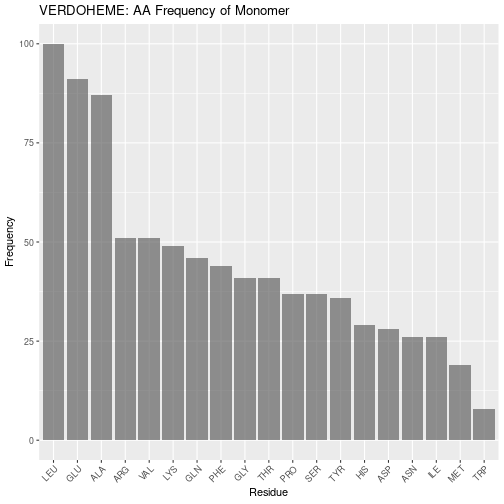
\includegraphics{_main_files/figure-latex/VERDOHEME-AAfreqAll-1.pdf}
\caption{\label{fig:VERDOHEME-AAfreqAll}VERDOHEME: AA Frequency of Monomer}
\end{figure}

Besides the frequencies of leucine and alanine, which have been found for heme-b and heme-c above to be highly frequent in hemoproteins at large, the frequency profiles for the verdoheme binding environment and monomers is shown to be quite dissimilar, supporting the results for the binding environment as unique, not simply due to background frequency.

\hypertarget{aa-distribution-over-distance}{%
\subsubsection{AA Distribution over distance}\label{aa-distribution-over-distance}}

The low sample size for verdoheme leads here to a poor figure with few residues plotted. This is likely attributable to an insufficient amount of distances and residues to cross-reference against each other, as occurs for all similar graphs. Regardless, the data that are plotted will be discussed.

The highly conserved histidine for hemoproteins is exclusively within 5A for verdoheme. This result again suggests that at least some of the data for verdoheme may be highly biased because of the small sample size - heme-b data included a greater range for histidine. The close proximity of glycine to verdoheme is also unexpected and unable to be explained without further study. The remainder of the residues plotted appear to follow the trends seen in for the other types of heme, distance values centered around 6A.

\begin{figure}
\centering
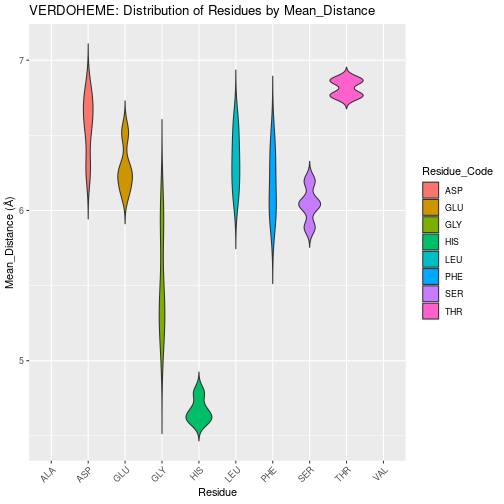
\includegraphics{_main_files/figure-latex/VERDOHEME-AAdist-1.pdf}
\caption{\label{fig:VERDOHEME-AAdist}VERDOHEME: AA Distances}
\end{figure}

\hypertarget{siroheme-1}{%
\subsection{Siroheme}\label{siroheme-1}}

\begin{figure}
\centering
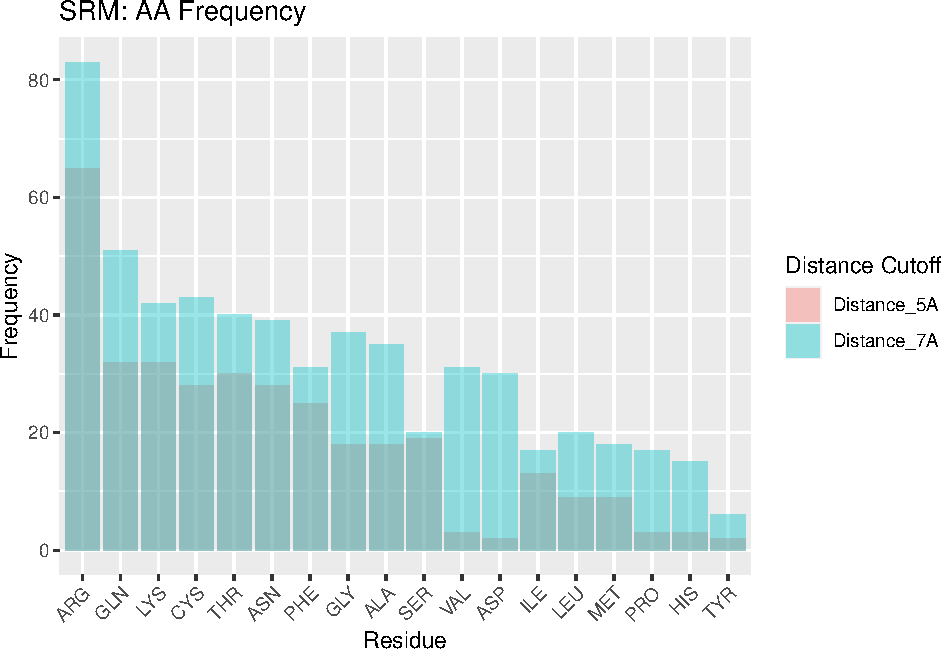
\includegraphics{_main_files/figure-latex/SRM-AAfreq-1.pdf}
\caption{\label{fig:SRM-AAfreq}SRM: AA Frequency}
\end{figure}

\begin{longtable}[t]{lr}
\caption{\label{tab:SRM-t-AAfreq}SRM AA Freq}\\
\toprule
Residue & Freq\\
\midrule
\endfirsthead
\caption[]{\label{tab:SRM-t-AAfreq}SRM AA Freq \textit{(continued)}}\\
\toprule
Residue & Freq\\
\midrule
\endhead

\endfoot
\bottomrule
\endlastfoot
\cellcolor{gray!6}{ARG} & \cellcolor{gray!6}{83}\\
GLN & 51\\
\cellcolor{gray!6}{CYS} & \cellcolor{gray!6}{43}\\
LYS & 42\\
\cellcolor{gray!6}{THR} & \cellcolor{gray!6}{40}\\
\addlinespace
ASN & 39\\
\cellcolor{gray!6}{GLY} & \cellcolor{gray!6}{37}\\
ALA & 35\\
\cellcolor{gray!6}{PHE} & \cellcolor{gray!6}{31}\\
VAL & 31\\
\addlinespace
\cellcolor{gray!6}{ASP} & \cellcolor{gray!6}{30}\\
LEU & 20\\
\cellcolor{gray!6}{SER} & \cellcolor{gray!6}{20}\\
MET & 18\\
\cellcolor{gray!6}{ILE} & \cellcolor{gray!6}{17}\\
\addlinespace
PRO & 17\\
\cellcolor{gray!6}{HIS} & \cellcolor{gray!6}{15}\\
TRP & 10\\
\cellcolor{gray!6}{TYR} & \cellcolor{gray!6}{6}\\
GLU & 2\\*
\end{longtable}

Siroheme, with a structure highly dissimilar to the other heme molecules examined, should be expected to have a different amino acid frequency profile - and indeed we confirm this in our results.

Nonpolar residues are not the most abundant in the siroheme binding pocket. In fact, disproportionately frequent to the rest of the residues in the binding pocket is arginine. Siroheme is saturated with carboxyl and propionate groups; the entire porphyrin ring surrounded by polar, electronegative groups. And therefore a polar, positively charged amino acid such as arginine is reasonable to expect in the binding pocket - what is striking, however is the extreme preference for arginine; such a profile does not exist for the other hemes. This is, however, sensible, siroheme contains propionate groups that likely still form polar interactions with arginine salt bridges, and the carboxyl groups may also form polar interactions with arginine.

Arginine is followed by other polar amino acids: glutamine, cystine, lysine, threonine, and asparagine; a more homogenous trend than seen for the other heme molecules, in that the trend is not interrupted as for other types of heme. Though these results could be expected, they demonstrate the extent to which siroheme's binding pocket is dominated by polar residues. The preference for arginine out of all polar amino acids may be attributed to its positive charge, and ability to form salt bridges that interact with the propionate groups; lysine also has a positive charge and a low pKa but is not capable of the latter interaction. Cysteine is used to coordinate the iron of siroheme, and while this did not significantly affect the frequency for other heme molecules, it is still possible this increases the value for cysteine for siroheme.

After this group of polar amino acids, glycine is the next most frequent. Glycine has been situated at about a median frequency for other heme molecules, so perhaps its frequency here, slightly above the median, is of note. Again, for glycine in particular, the reason for its particular frequency cannot be determined from this data, but it appears to have some role.

Finally we come to several nonpolar amino acids: alanine, phenylalanine, and valine. These amino acids define roughly the median of the frequency data. With all the polar groups on siroheme, it might be expected that only polar interactions would be desirable. However, the not miniscule frequency of these residues suggests nonpolar interactions still occur in the binding pocket; the porphyrin ring remains, as well as methyl groups and the small nonpolar portion of the carboxyl and propionate groups. It is perhaps in these areas that the nonpolar residues interact.

After these nonpolar residues the remaining frequencies do not follow a clear trend but regardless are discussed. After aspartate the remaining frequencies are considerably lower. This may be an artefact of a small sample size, or may suggest the remaining residues form, if any, less favorable interactions with the heme.

Aspartate appears next most frequently; it is a polar, negatively charged amino acid (at pH 7). Siroheme is saturated with other electronegative groups; perhaps there is some repulsion between these groups and aspartate -- this could explain why, despite being a polar residue, arginine does not appear very frequently in the binding pocket.

Leucine is the first of the residues of diminished frequency. It is nonpolar. It, and, skipping a frequency, methionine, isoleucine, and proline, appear less frequently, and therefore are likely disfavored from forming the relatively few nonpolar interactions that do occur. Why is not clear - other small, nonpolar residues, and other lengthy nonpolar residues appear in the pocket in greater frequency.

Serine appears just less frequently than leucine, and in this context may likely be considered a polar residue that is not as strongly polar or positively charged and therefore less preferred to include in the binding pocket to form polar interactions with siroheme as other residues.

Histidine appears quite infrequently. As with siroheme, other, more strongly polar and perhaps less bulky residues are likely preferred.

Tryptophan is the least frequent nonpolar residue. The presence of a weak hydrogen bond and its size may preclude its inclusion in the binding pocket in lieu of more uniformly nonpolar residues that take up less space.

Tyrosine and glutamate are the least frequent polar residues. This is in stark opposition to the other heme molecules - tyrosine seemed to be favored for other heme molecules to form interactions with the propionate groups. Glutamate is also extremely infrequent, even in spite of its similarity to aspartate. Both are electronegative at pH 7 - glutamate's extra carbon may provide sufficient steric hindrance to render it less favored. In either case, the infrequency of these residues and the tendencies of other, more intensely polar or nonpolar amino acids to be more populous, suggests tyrosine and glutamate, in the siroheme binding environment, do not interact strongly enough to be favored over other polar residues.

\hypertarget{comparing-to-srm-aa-background-freq}{%
\subsubsection{Comparing to SRM AA Background Freq}\label{comparing-to-srm-aa-background-freq}}

\begin{figure}
\centering
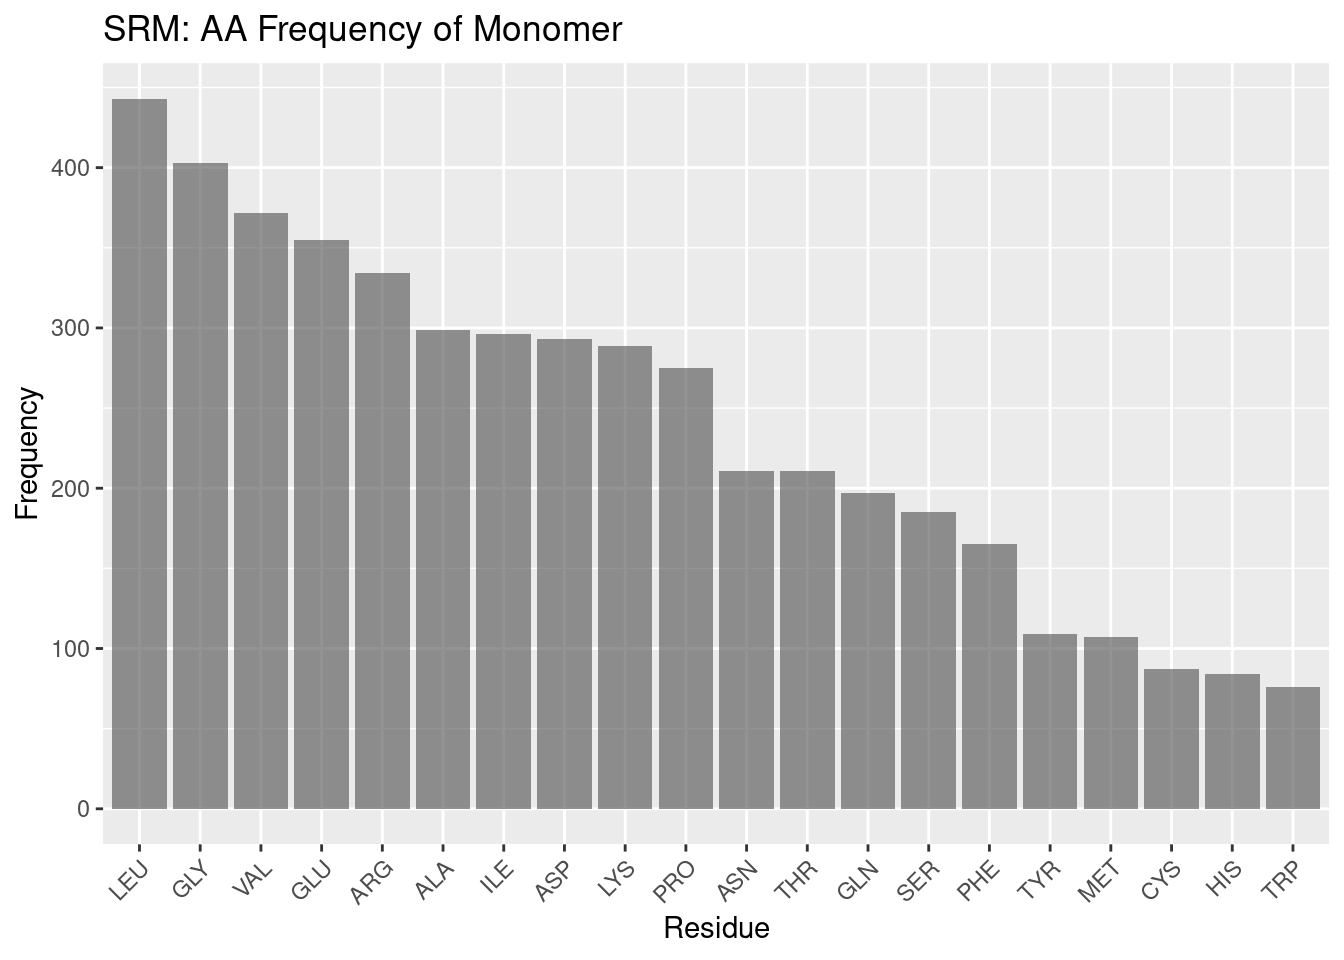
\includegraphics{_main_files/figure-latex/SRM-AAfreqAll-1.pdf}
\caption{\label{fig:SRM-AAfreqAll}SRM: AA Frequency of Monomer}
\end{figure}

Compared to the other heme molecules, siroheme's binding pocket amino acid frequencies are even more different than the background frequencies. Arginine is far and away the most frequent amino acid in the binding pocket; leucine is the most populous amino acid in the monomer overall, seeming to follow a trend amongst the hemoproteins examined so far. Again, discussing the remainder of the frequencies of the monomer would be pure conjecture, but it is worthwhile to note that the pocket frequencies appear unique against the background.

\hypertarget{distance-stuff}{%
\subsubsection{Distance stuff}\label{distance-stuff}}

Residues appear less uniformly distributed over distance for siroheme binding pockets when compared against the distribution for other heme molecules. Cysteine is the only residue that comes within 5A of siroheme; it is used to coordinate the iron in siroheme, so this result is expected. The lack of other residues being within 5A, differing from other heme molecules, suggests the many carboxyl and propionate groups on siroheme prevent, or preclude the need for closer interaction except for coordinating residues.

\begin{figure}
\centering
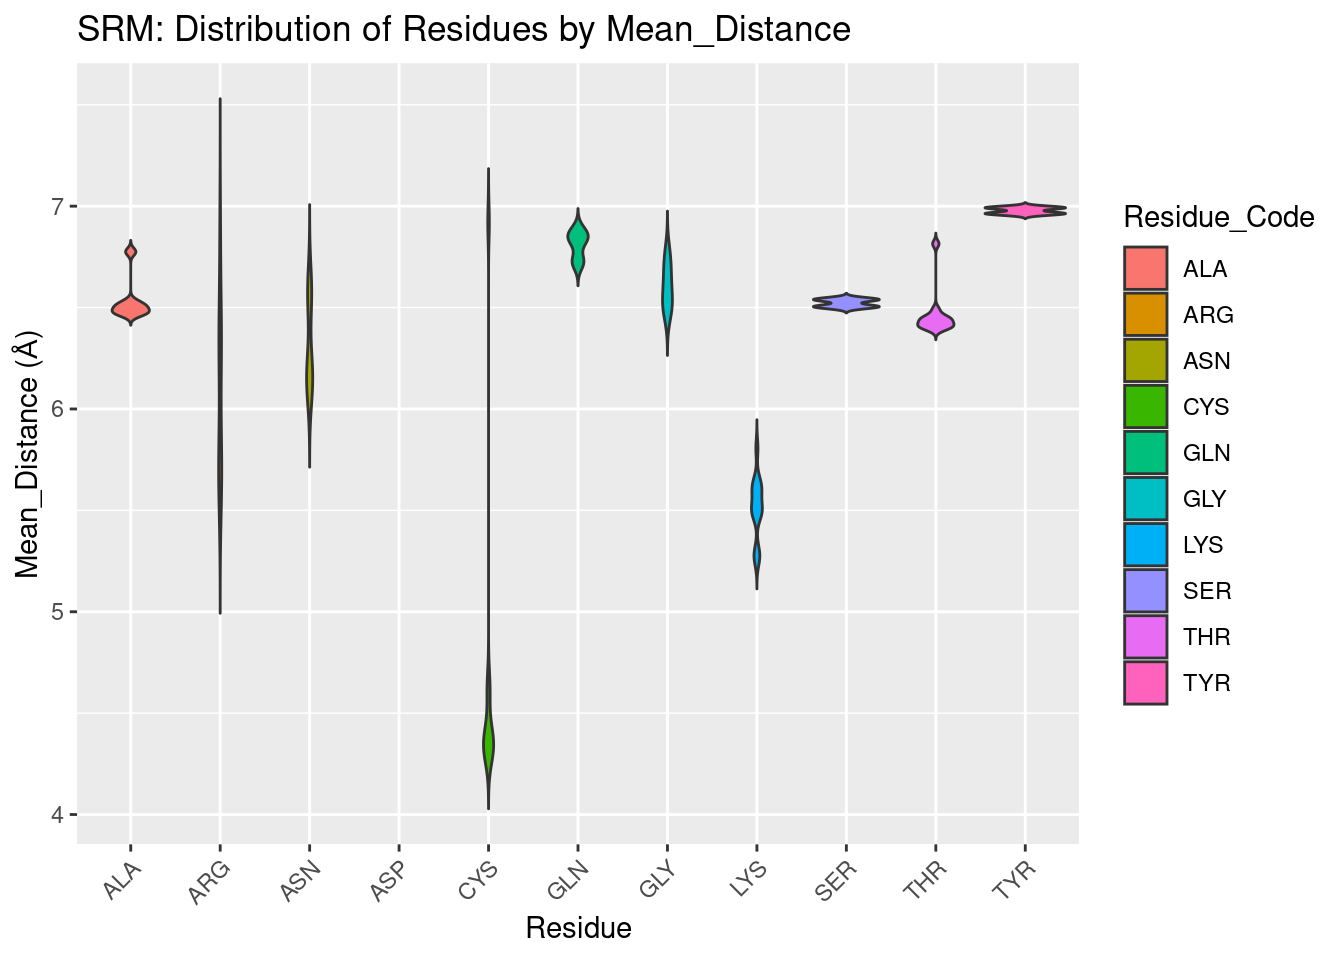
\includegraphics{_main_files/figure-latex/SRM-AAdist-1.pdf}
\caption{\label{fig:SRM-AAdist}SRM: AA Distances}
\end{figure}

\hypertarget{volume-discussion}{%
\section{Volume Discussion}\label{volume-discussion}}

Figures can be found in Appendix \ref{figs-vol}.

Volume results were rather spread out, with close agreement only found for heme-b. In general, volume for all heme molecules regardless of distance cutoff centered at approximately 1200 A³. This result may be useful in protein engineering efforts, especially for selection or design of binding pockets.

\hypertarget{surface-areas}{%
\section{Surface Areas}\label{surface-areas}}

\hypertarget{surface-area-of-heme-molecules}{%
\subsection{Surface Area of Heme Molecules}\label{surface-area-of-heme-molecules}}

Both solvent accessible and solvent excluded surface areas were calculated for heme molecules and binding pockets. The differences between these two measures was discussed in Section (FIXME). The results are extremely similar for solvent accessible and solvent excluded surface areas; and therefore only solvent accessible surface area, a measure more practically interpreted into chemical phenomena, is discussed below. Figures and data for solvent excluded surface areas are available in Appendix (FIXME: insert reference).

The solvent accessible surface area for all heme \emph{molecules} themselves centers around values of 1000 A². This result is reasonable, given the similarity in size and structure of all heme molecules, in spite of the attached groups. Figures are shown below; extreme outliers have been removed from these figures but full data tables are available in (FIXME add appendix number). The outliers are likely artefacts of the method used to calculate surface area and potential conflicts with the method used to convert multimeric proteins to monomers.

\hypertarget{surface-area-of-binding-pockets}{%
\section{Surface Area of Binding Pockets}\label{surface-area-of-binding-pockets}}

The surface area of binding pockets is more varied than the heme surface areas.

Heme-b and verdoheme, being highly similar molecules, with the same propionate groups, and one the derivative of the other, have quite similar surface areas, centering around 10,000-11,000 A². This is useful as a baseline to discuss the surface area of the binding pockets of the other two heme molecules below.

The surface area of the binding pocket of heme-c is considerably lower than that of heme-b and verdoheme. Its values center around 7500 A². Heme-c is bound covalently to the hemoprotein, forming thioether bonds with cysteine residues at two sites; this result suggests that the covalent bonds may exclude these sites from interacting with water molecules. Further study would be required to confirm this phenomenon.

The surface area of siroheme's binding pocket is far greater than that for other heme molecules: values center around 21000 A². Siroheme's extra groups on the porphyrin ring do not appear to affect its own surface area, per above. However, it is effectively a very polar molecule and appropriately the binding pocket is highly saturated with very polar amino acids, as seen in the amino acid frequency analysis. The binding pocket is therefore completely different from the other heme molecules, and these populous, polar amino acids favorably interact with aqueous solvent, negating the need to bury any hydrophobic residues and reduce surface area.

\hypertarget{angular-data}{%
\section{Angular Data}\label{angular-data}}

As briefly mentioned in the introduction, angular data was generated but will not be discussed extensively. Figures and data tables may be found in Appendix (FIXME). Amongst the results are tight distributions of planar angles and CA-CB-Fe angles for some residues nearby and far away from heme; but much of the data demonstrates a broad range of angles that may be formed. The data may be useful for protein engineering and residue placement, but cannot be productively discussed and are therefore relegated to the appendices.

\hypertarget{limitations-of-the-study}{%
\section{Limitations of the Study}\label{limitations-of-the-study}}

A high throughput framework was built to conduct this study. However, guaranteeing the quality of PDBs to enable the scripts to functon properly proved challenging, and the sample size is small, although diverse. This problem only exists for heme-b and heme-c -- for siroheme and verdoheme, all structures in the PDB capable of being used, were used. Heme-b and heme-c would only require more trial and error, or preprocessing, to be input to the framework that has been built.

Although many hypotheses have been suggested in the discussion to explain the data, limited experimental data exists to confirm them. Future work may include wet lab experiments to confirm these hypotheses, such as mutating several hemoproteins to contain higher or lower pecentages of nonpolar residues in the binding pocket, and observing how the binding of heme is affected.

Some of these data could also be analyzed more thoroughly, for example eliminating the coordinating amino acids from the amino acid frequency data. This was not possible here due to how the framework is constructed: coordinating residues are not identified, nor is a definition proposed to identify coordinating residues. Manual input of known coordinating residues would be necessary to be certain that they could be eliminated from the final dataset analyzed, but this was beyond the scope of this study.

UCSF-Chimera was used to generate all data used in this study; many algorithms have remained unchanged for some time (surface area calculations are sourced from MSMS (1996) and volume calculations from surfnet (1995)). It would be ideal to compare with any new algorithms that are developed to calculate surface area or volume, or with any experimental data that may be used confirm these numbers.

The reason being for this desired orthogonality is that the algorithms themselves may certainly introduce bias based off how they work. Surfnet generates 3D-contour surfaces to identify cavities; in practice, many small ``bubbles'' or insignificant cavities were generated in the study, and are filtered out during analysis -- the parameters chosen can also significantly influence the behavior of the algorithm; in this study, the default parameters appeared to generate the most reasonable binding pocket. But this assessment is based off subjective visual observation by the author, and therefore introduces further bias. One may expect applying the same algorithm with the same parameters to many PDBs may at least introduce the same bias to all samples, but the algorithm may distort some PDBs more than others depending on the shape and size of their binding pocket.

\adjustmtc
\markboth{Methods}{}

\hypertarget{conclusion}{%
\chapter{Conclusion}\label{conclusion}}

A knowledge gap in the binding environment for heme exists in the present literature. A high-throughput framework employing UCSF Chimera was constructed to process diverse sets of hemoproteins and output information about their binding pockets: amino acid frequencies and distances from heme, volume, surface area, angles. Data was gathered and predicted from representative and varied datasets for heme-b, heme-c, verdoheme, and siroheme, and their respective hemoproteins. R was used to analyze all data.

The results of this study are suggest that binding pockets for hemoproteins have some requirements for binding that may have been overlooked to date. The data and their trends observed in this study demonstrate several phenomena.

First, the heme binding environments for heme-b, heme-c, and verdoheme contain high populations of nonpolar amino acids, suggesting nonpolar interactions may be of greater importance than previously thought to providing the necessary interactions to bind heme. The binding environment for siroheme, by contrast, is shown to be extremely enriched with polar amino acids, which is not very surprising; but this binding environment also still contains many nonpolar amino acids, reinforcing the idea that the polar interactions for all heme molecules, while necessary, may be insufficient for heme binding.

Second, most of the volume data for the binding pockets of all heme molecules centers around a value of 1200 A³. Surface areas of heme-b and verdoheme binding pockets are similar, approximately 10000 A², the surface area for heme-c is less, approximately 7500 A², and for siroheme is approximately 21000 A². These values may be useful in the design of artifical metalloenzymes.

Additionally, the seeming conservation of the volume size but the variety in pocket surface areas demonstrates that while the heme molecules may be of similar size and, besides attached groups, similar structure, the attached groups will significantly affect what interactions occur in the binding pockets, and therefore the shape and exposure to solvent in the binding pockets. Siroheme is strongly polar and its binding pocket has a large surface area and is therefore highly solvent exposed, as compared to heme-b which has more nonpolar groups that must be buried and therefore requiring a smaller surface area.

Finally, angular data were generated; but the phenomena observed, such as some residues having tight ranges of angles in relation to heme or the heme iron, cannot be interpreted as useful results, except perhaps for some protein engineering efforts that may have interest in the range of possible angles for a specific residue.

These results may be useful for the rational design of hemoproteins, with the importance of nonpolar interactions in particular likely of great interest. The framework constructed for this study can be applied to any list of PDBs and their respective ligands, thereby facilitating similar research for other proteins.

\startappendices

\hypertarget{a-figures}{%
\chapter{Figures}\label{a-figures}}

\minitoc

\hypertarget{figs-aaFreqOverlaid}{%
\section{AA Frequency}\label{figs-aaFreqOverlaid}}

\begin{figure}
\centering
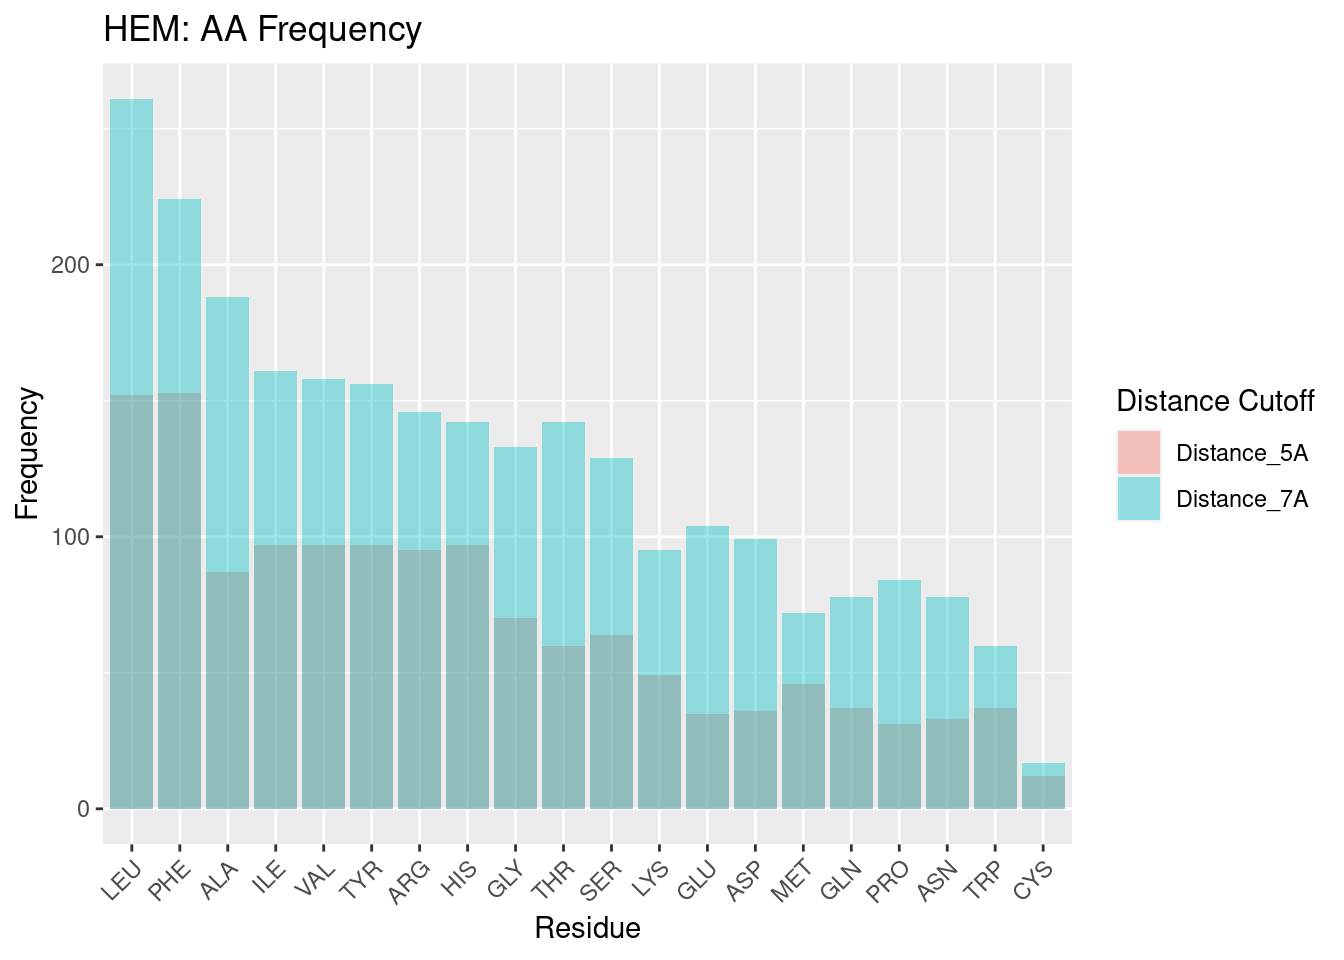
\includegraphics{_main_files/figure-latex/HEM-AAfreqOverlaid-1.pdf}
\caption{\label{fig:HEM-AAfreqOverlaid}HEM: AA Frequency}
\end{figure}

\begin{figure}
\centering
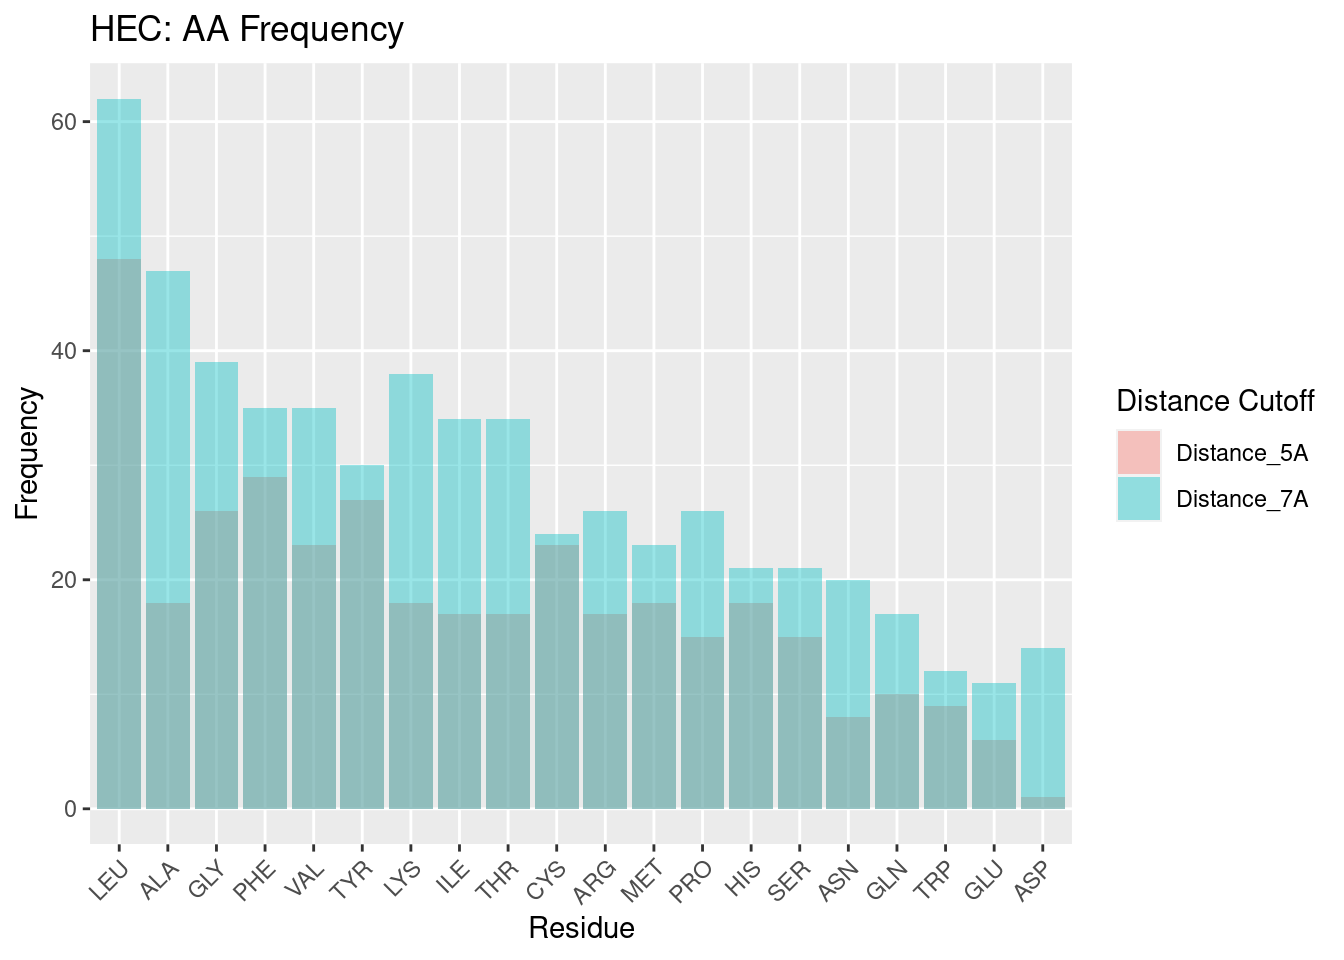
\includegraphics{_main_files/figure-latex/HEC-AAfreqOverlaid-1.pdf}
\caption{\label{fig:HEC-AAfreqOverlaid}HEC: AA Frequency}
\end{figure}

\begin{figure}
\centering
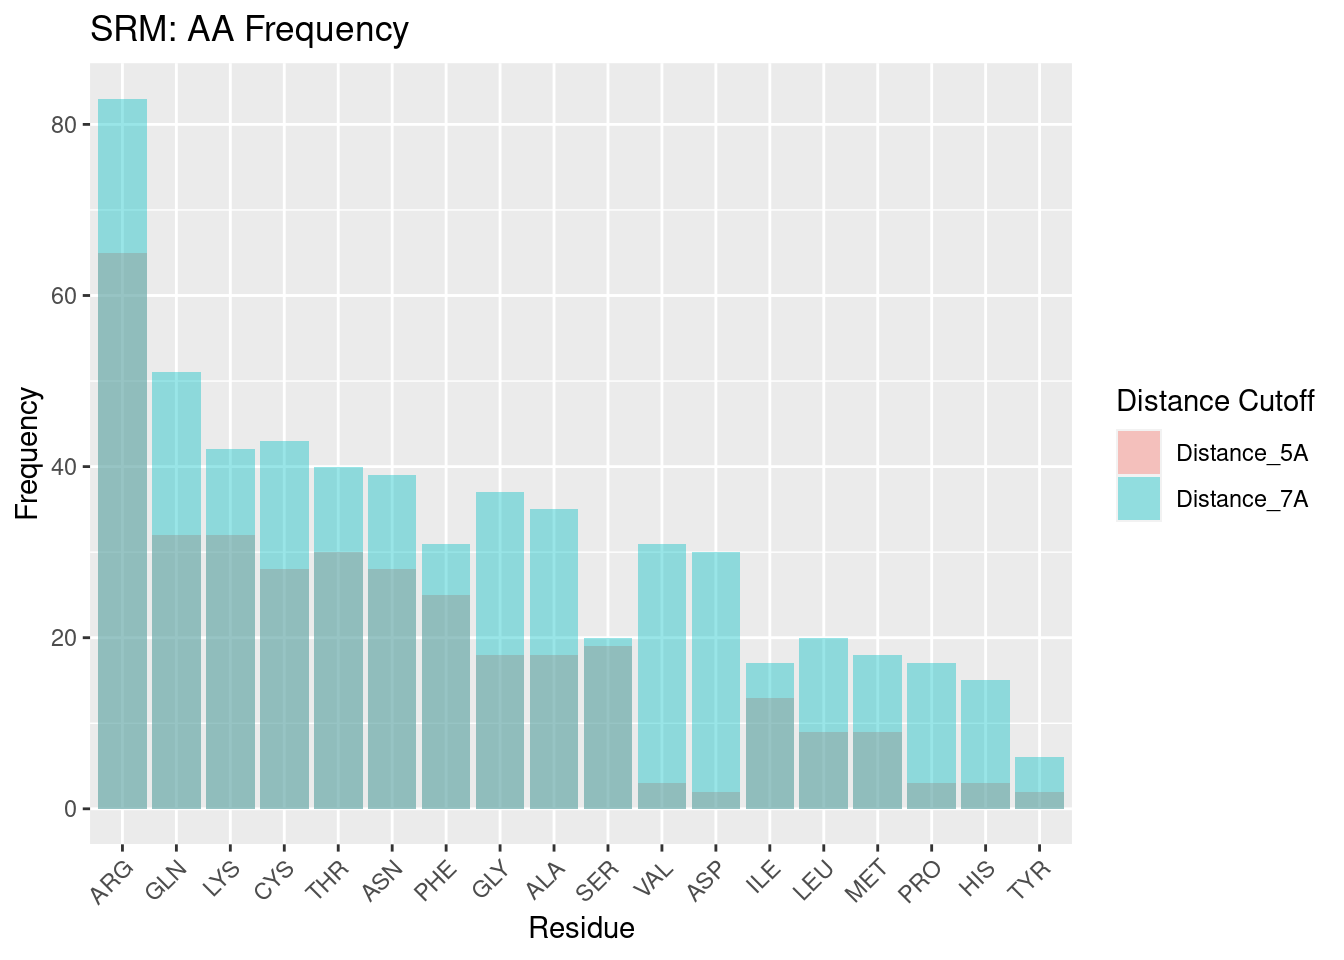
\includegraphics{_main_files/figure-latex/SRM-AAfreqOverlaid-1.pdf}
\caption{\label{fig:SRM-AAfreqOverlaid}SRM: AA Frequency}
\end{figure}

\begin{figure}
\centering
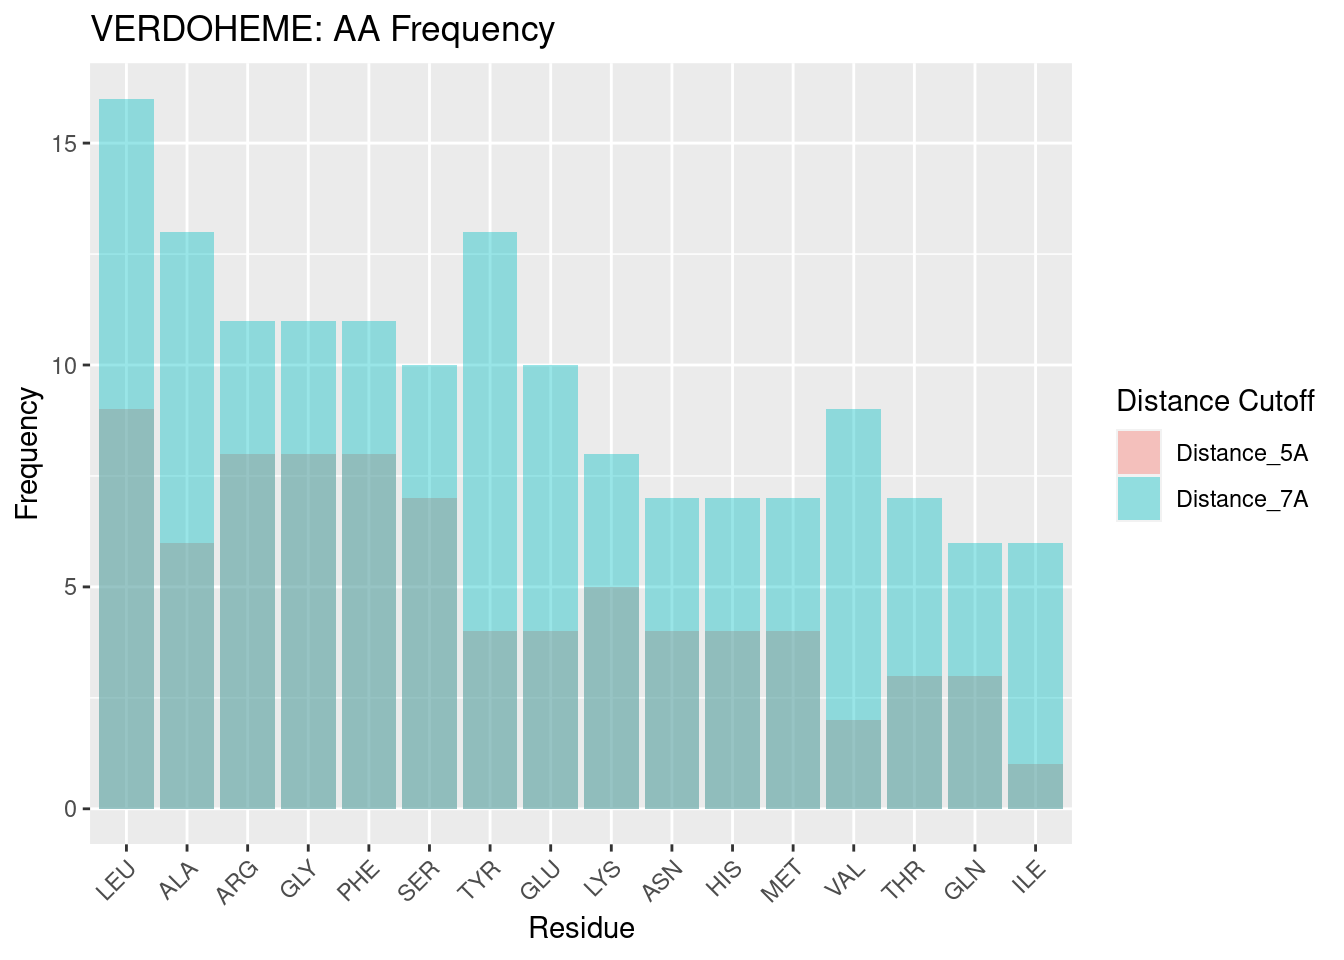
\includegraphics{_main_files/figure-latex/VERDOHEME-AAfreqOverlaid-1.pdf}
\caption{\label{fig:VERDOHEME-AAfreqOverlaid}VERDOHEME: AA Frequency}
\end{figure}

\hypertarget{figs-vol}{%
\section{Volume}\label{figs-vol}}

\begin{figure}
\centering
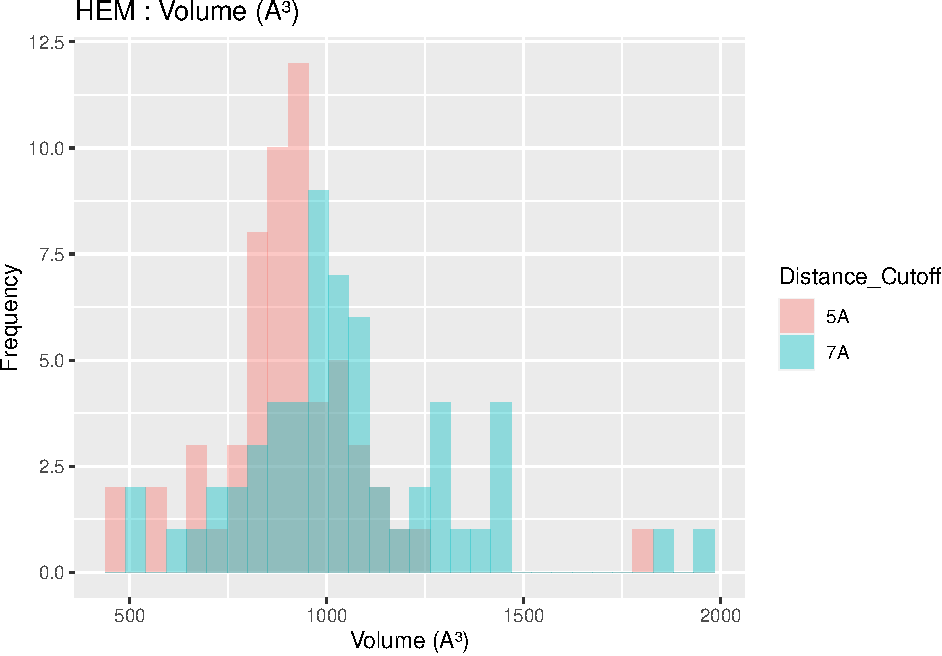
\includegraphics{_main_files/figure-latex/HEM-Volume-1.pdf}
\caption{\label{fig:HEM-Volume}HEM: Volume}
\end{figure}

\begin{figure}
\centering
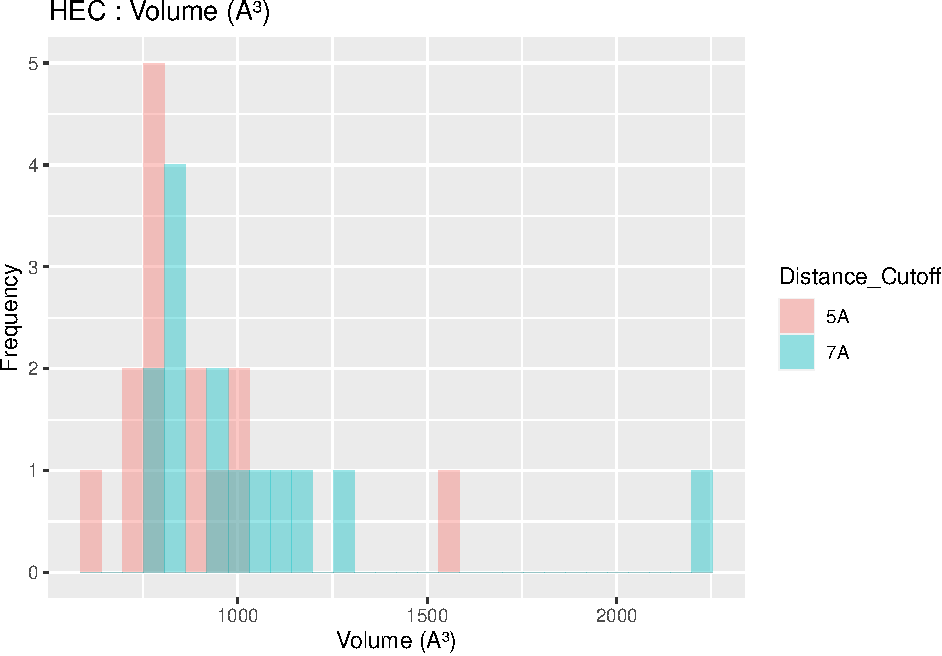
\includegraphics{_main_files/figure-latex/HEC-Volume-1.pdf}
\caption{\label{fig:HEC-Volume}HEC: Volume}
\end{figure}

\begin{figure}
\centering
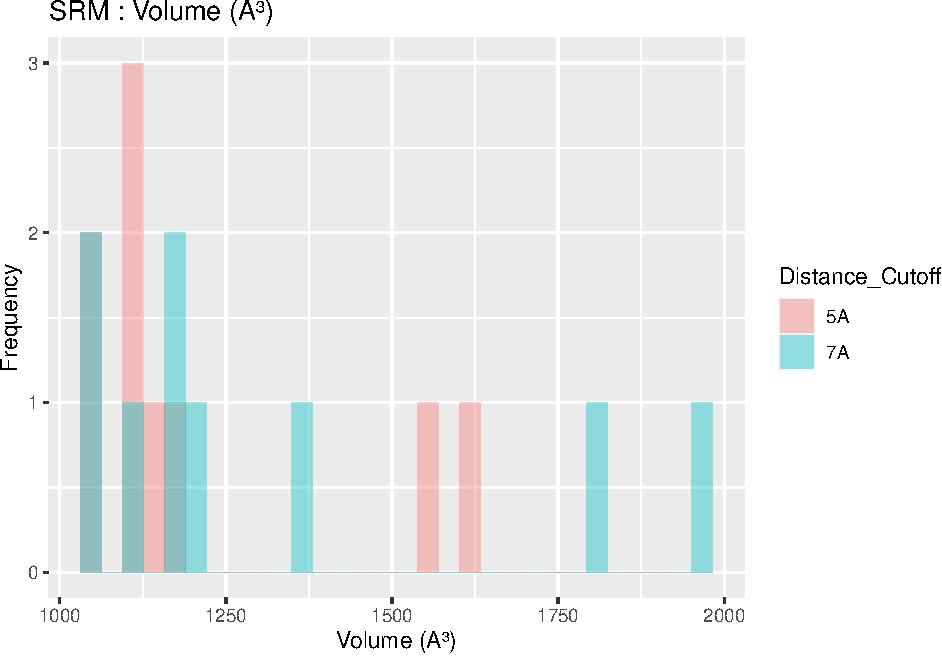
\includegraphics{_main_files/figure-latex/SRM-Volume-1.pdf}
\caption{\label{fig:SRM-Volume}SRM: Volume}
\end{figure}

\begin{figure}
\centering
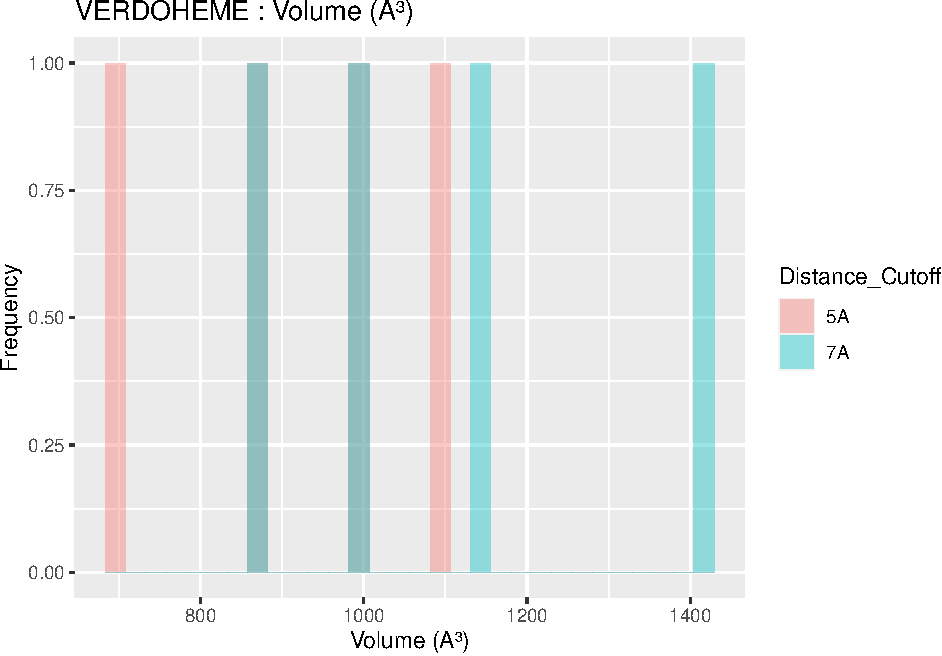
\includegraphics{_main_files/figure-latex/VERDOHEME-Volume-1.pdf}
\caption{\label{fig:VERDOHEME-Volume}VERDOHEME: Volume}
\end{figure}

\hypertarget{figs-ligExcSA}{%
\section{Ligand Excluded Surface Area}\label{figs-ligExcSA}}

\begin{figure}
\centering
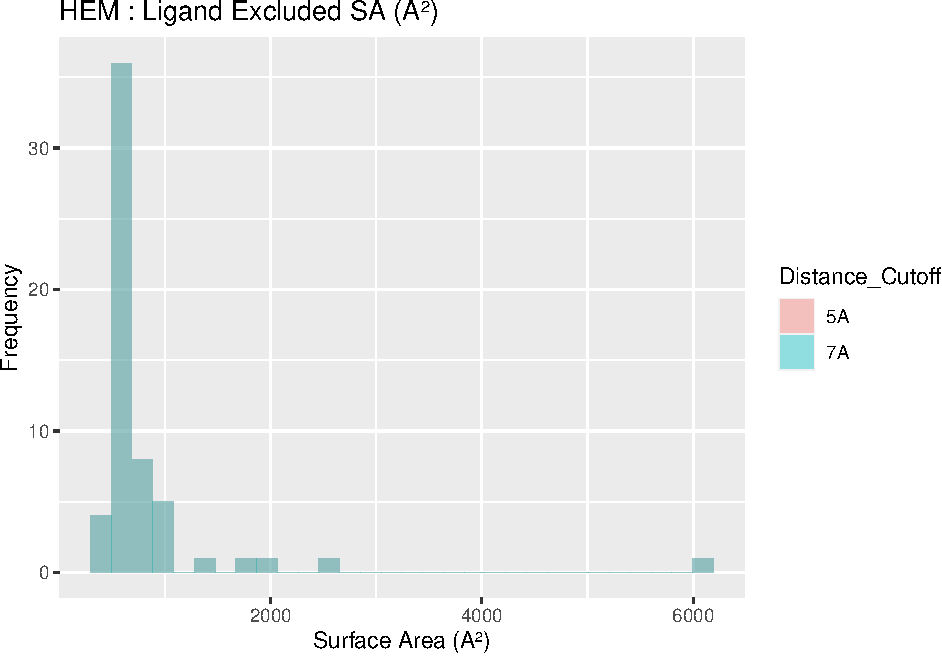
\includegraphics{_main_files/figure-latex/HEM-Ligand-ExcludedSA-1.pdf}
\caption{\label{fig:HEM-Ligand-ExcludedSA}HEM: Ligand Excluded Suface Area}
\end{figure}

\begin{figure}
\centering
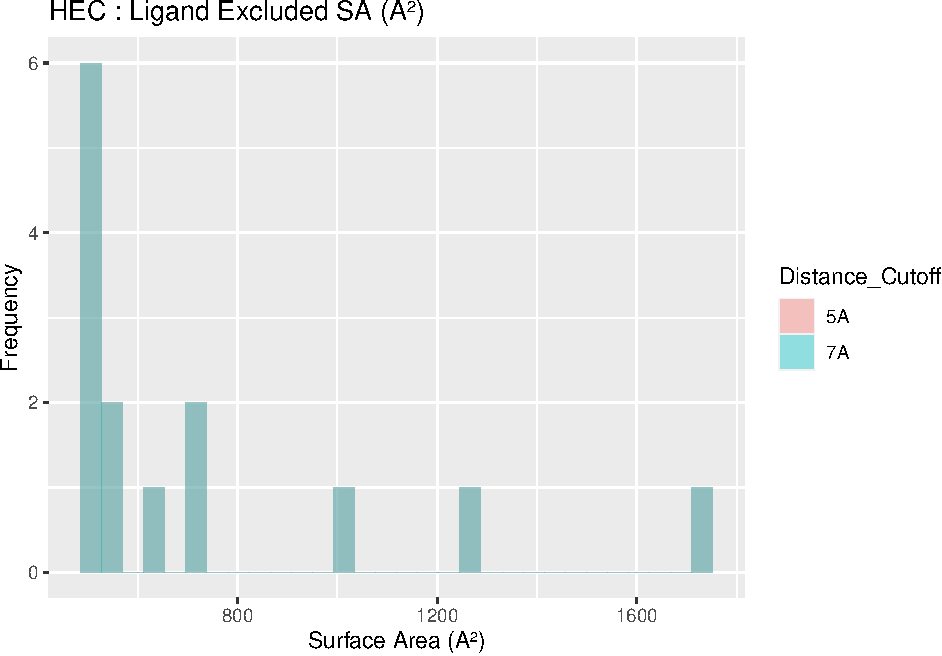
\includegraphics{_main_files/figure-latex/HEC-Ligand-ExcludedSA-1.pdf}
\caption{\label{fig:HEC-Ligand-ExcludedSA}HEC: Ligand Excluded Suface Area}
\end{figure}

\begin{figure}
\centering
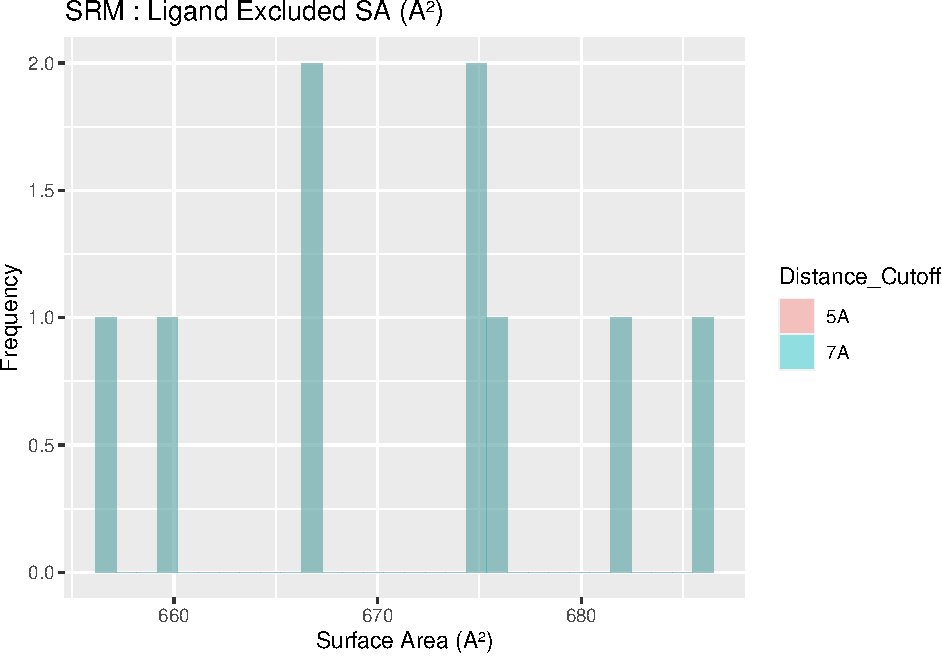
\includegraphics{_main_files/figure-latex/SRM-Ligand-ExcludedSA-1.pdf}
\caption{\label{fig:SRM-Ligand-ExcludedSA}SRM: Ligand Excluded Suface Area}
\end{figure}

\begin{figure}
\centering
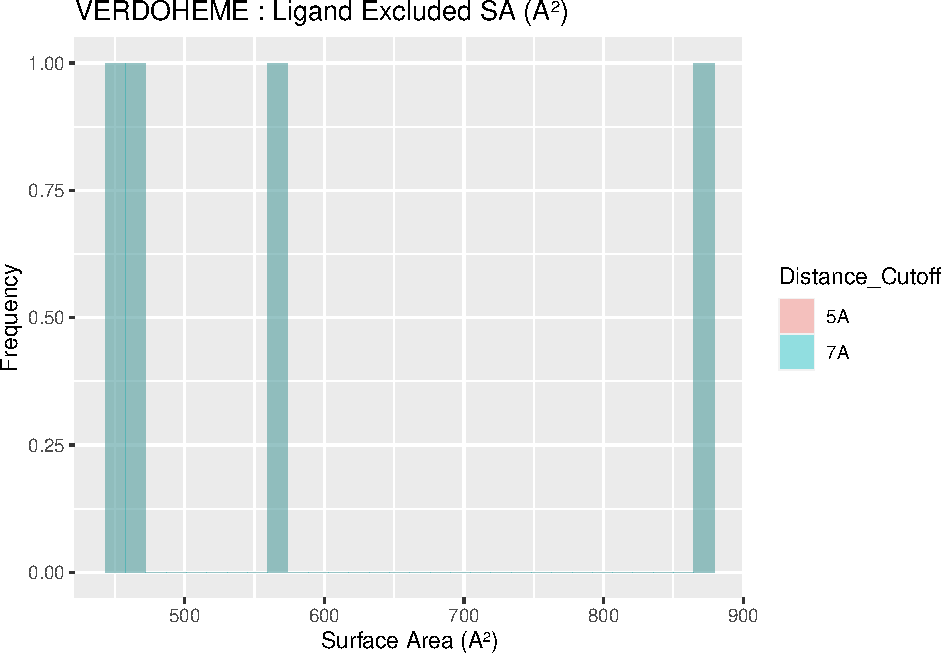
\includegraphics{_main_files/figure-latex/VERDOHEME-Ligand-ExcludedSA-1.pdf}
\caption{\label{fig:VERDOHEME-Ligand-ExcludedSA}VERDOHEME: Ligand Excluded Suface Area}
\end{figure}

\hypertarget{figs-ligAccSA}{%
\section{Ligand Accessible Surface Area}\label{figs-ligAccSA}}

\begin{figure}
\centering
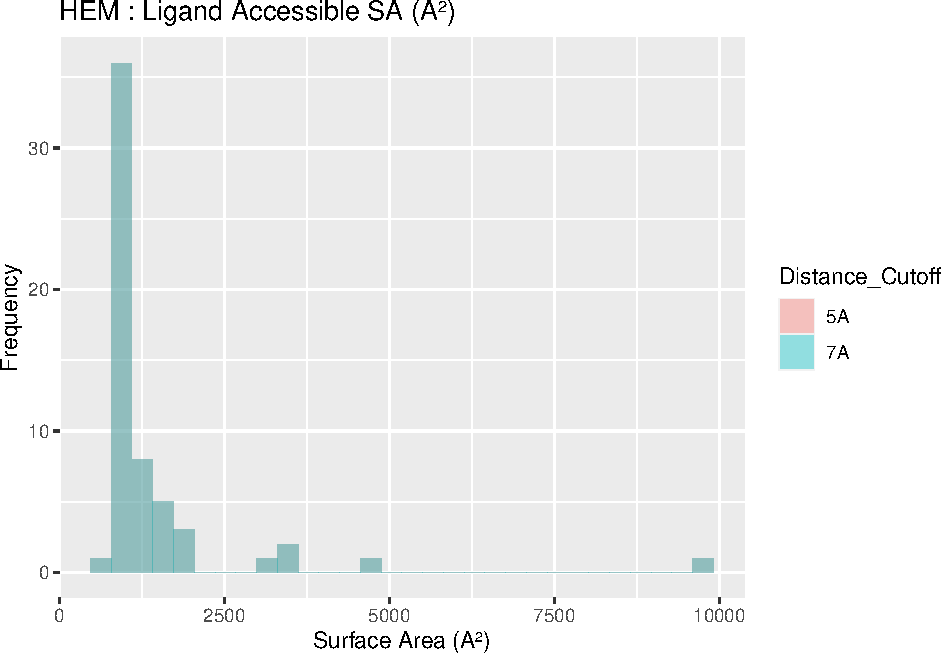
\includegraphics{_main_files/figure-latex/HEM-Ligand-AccessibleSA-1.pdf}
\caption{\label{fig:HEM-Ligand-AccessibleSA}HEM: Ligand Accessible Surface Area}
\end{figure}

\begin{figure}
\centering
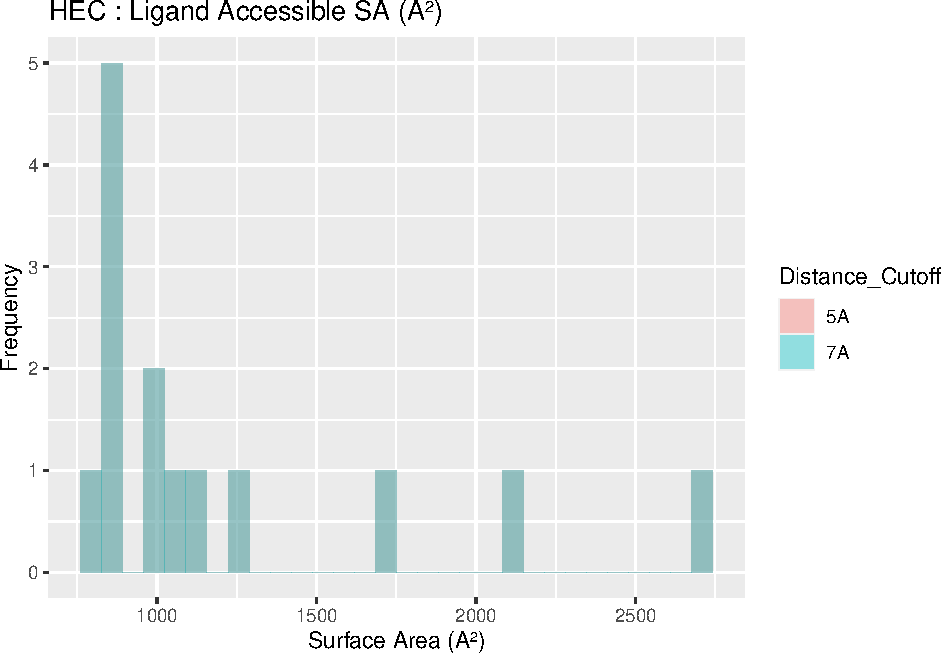
\includegraphics{_main_files/figure-latex/HEC-Ligand-AccessibleSA-1.pdf}
\caption{\label{fig:HEC-Ligand-AccessibleSA}HEC: Ligand Accessible Surface Area}
\end{figure}

\begin{figure}
\centering
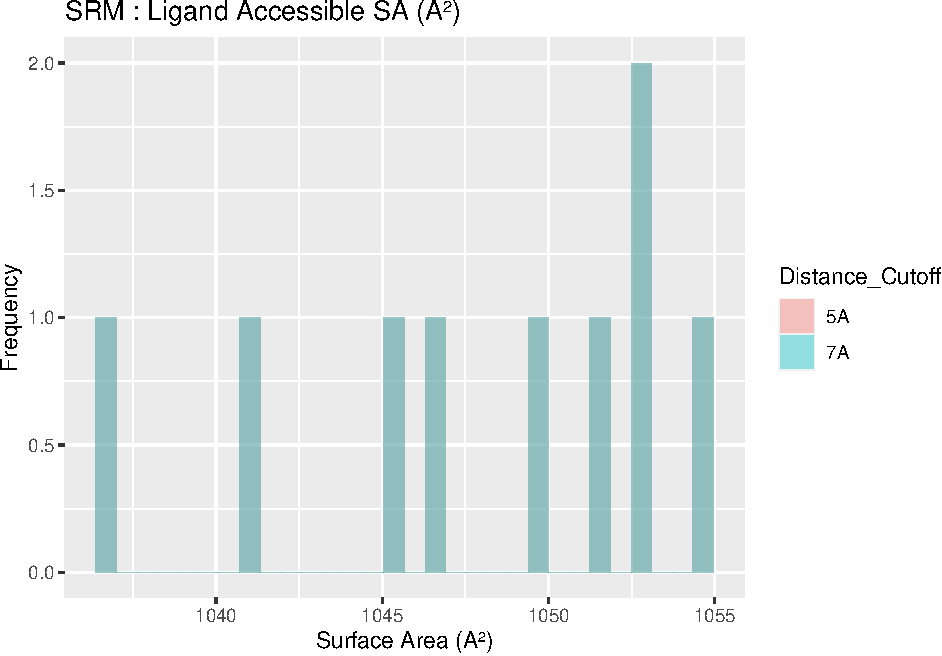
\includegraphics{_main_files/figure-latex/SRM-Ligand-AccessibleSA-1.pdf}
\caption{\label{fig:SRM-Ligand-AccessibleSA}SRM: Ligand Accessible Surface Area}
\end{figure}

\begin{figure}
\centering
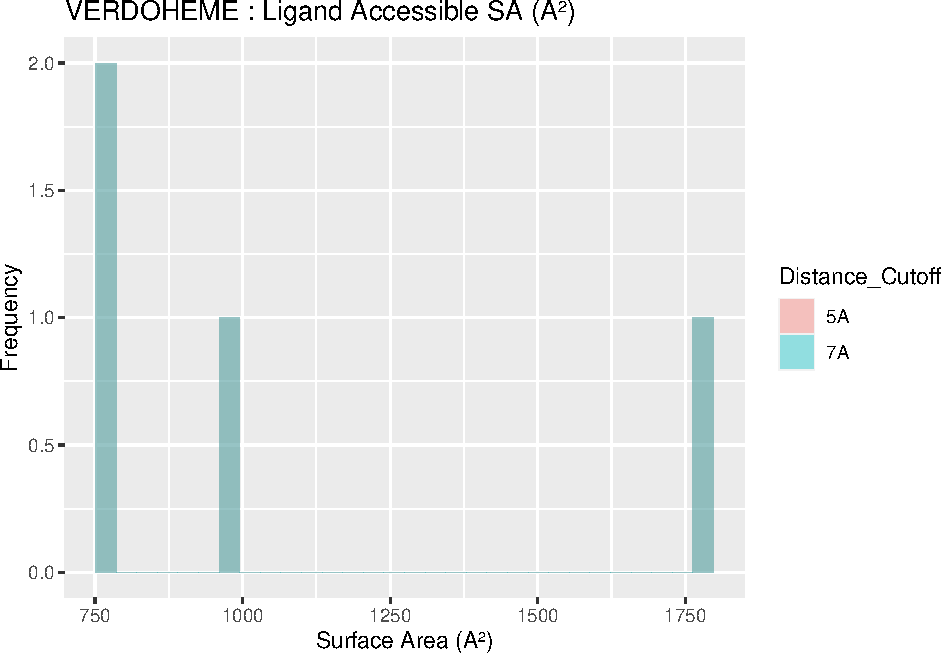
\includegraphics{_main_files/figure-latex/VERDOHEME-Ligand-AccessibleSA-1.pdf}
\caption{\label{fig:VERDOHEME-Ligand-AccessibleSA}VERDOHEME: Ligand Accessible Surface Area}
\end{figure}

\hypertarget{figs-pocketExcSA}{%
\section{Pocket Excluded Surface Area}\label{figs-pocketExcSA}}

\begin{figure}
\centering
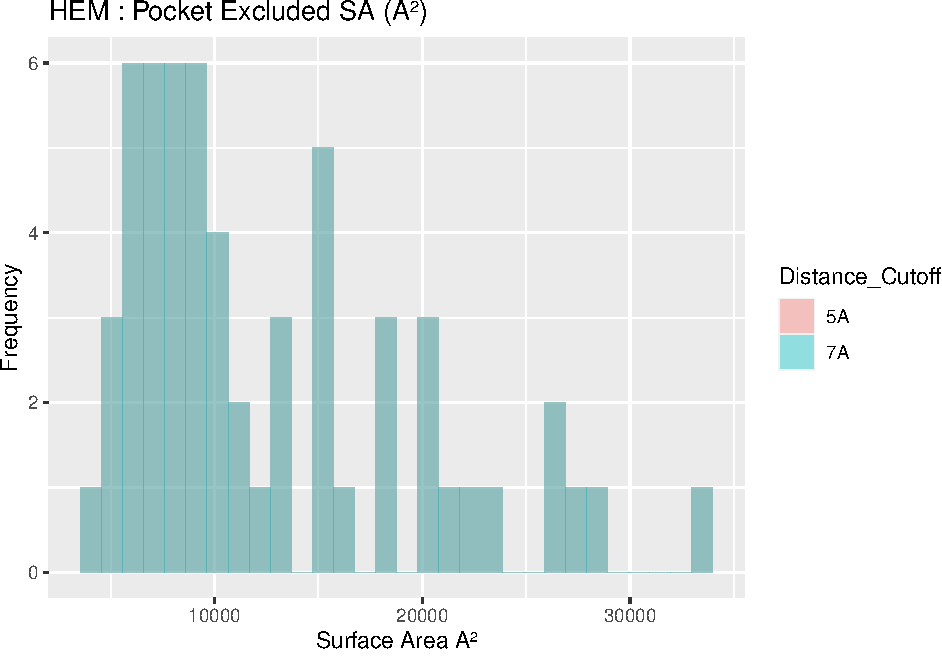
\includegraphics{_main_files/figure-latex/HEM-Pocket-ExcludedSA-1.pdf}
\caption{\label{fig:HEM-Pocket-ExcludedSA}HEM: Pocket Excluded Surface Area}
\end{figure}

\begin{figure}
\centering
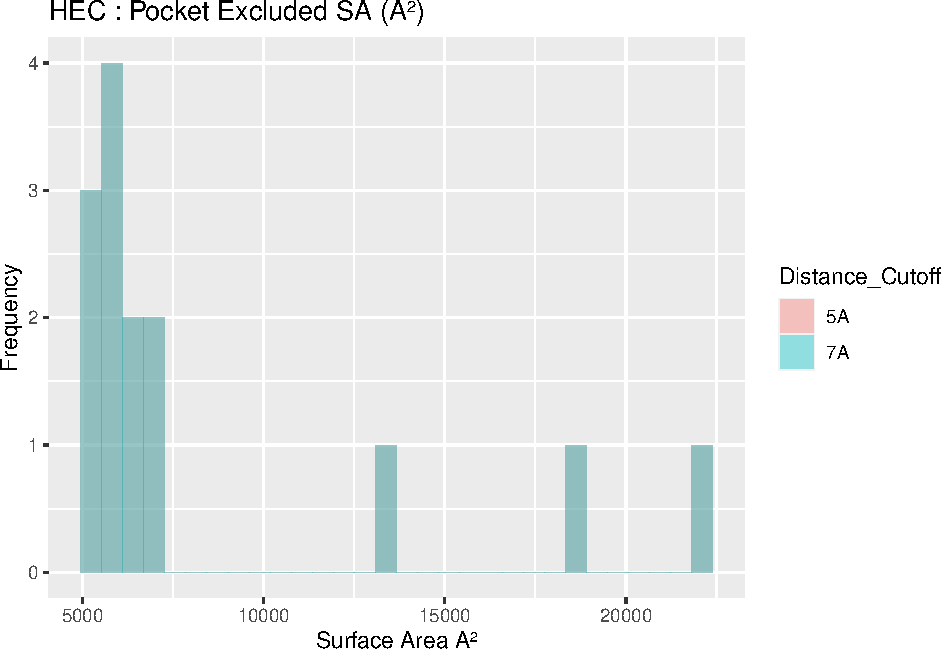
\includegraphics{_main_files/figure-latex/HEC-Pocket-ExcludedSA-1.pdf}
\caption{\label{fig:HEC-Pocket-ExcludedSA}HEC: Pocket Excluded Surface Area}
\end{figure}

\begin{figure}
\centering
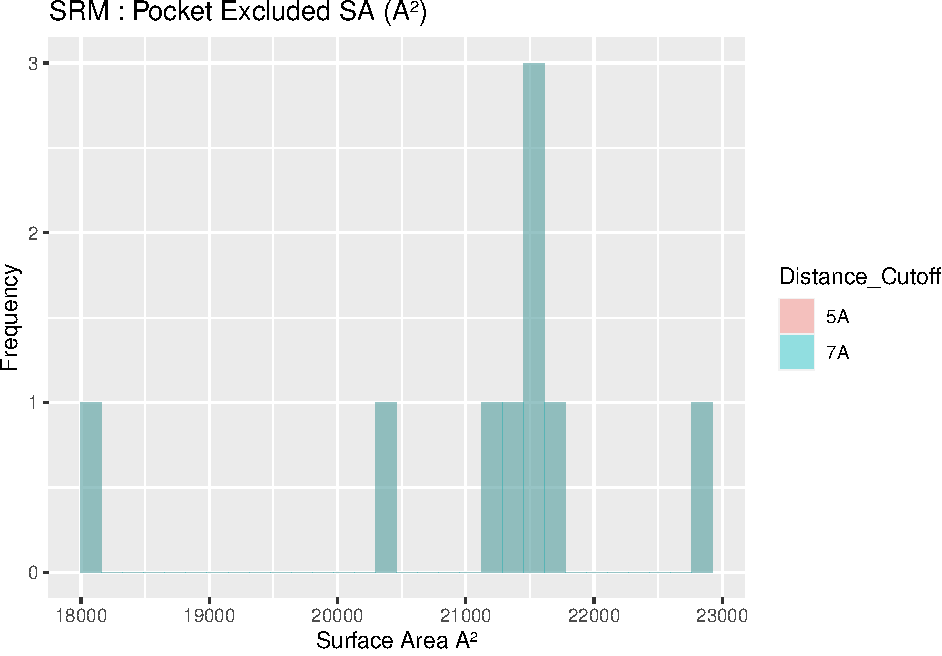
\includegraphics{_main_files/figure-latex/SRM-Pocket-ExcludedSA-1.pdf}
\caption{\label{fig:SRM-Pocket-ExcludedSA}SRM: Pocket Excluded Surface Area}
\end{figure}

\begin{figure}
\centering
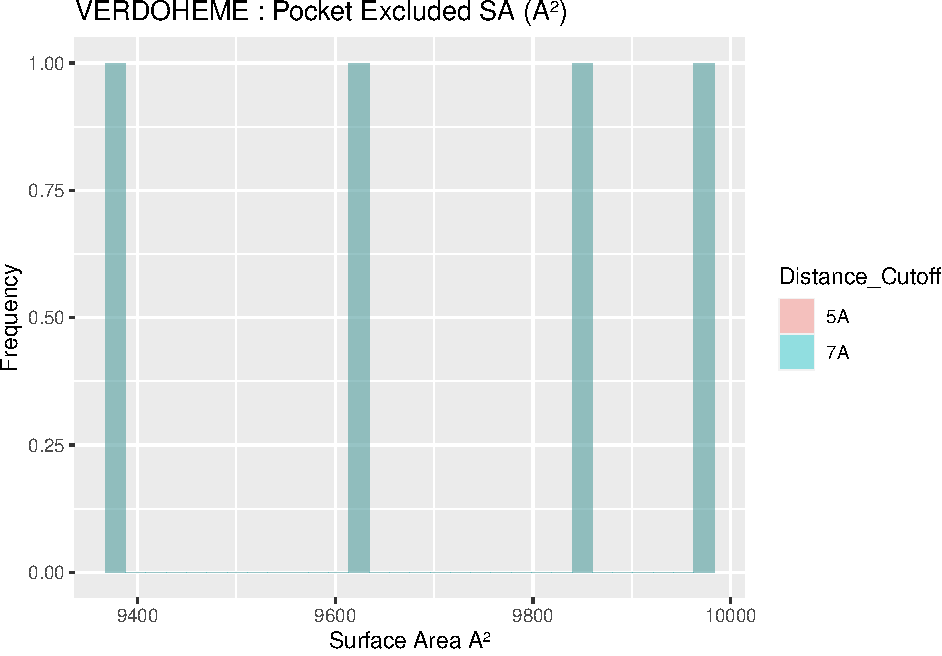
\includegraphics{_main_files/figure-latex/VERDOHEME-Pocket-ExcludedSA-1.pdf}
\caption{\label{fig:VERDOHEME-Pocket-ExcludedSA}VERDOHEME: Pocket Excluded Surface Area}
\end{figure}

\hypertarget{figs-pocketAccSA}{%
\section{Pocket Accessible Surface Area}\label{figs-pocketAccSA}}

\begin{figure}
\centering
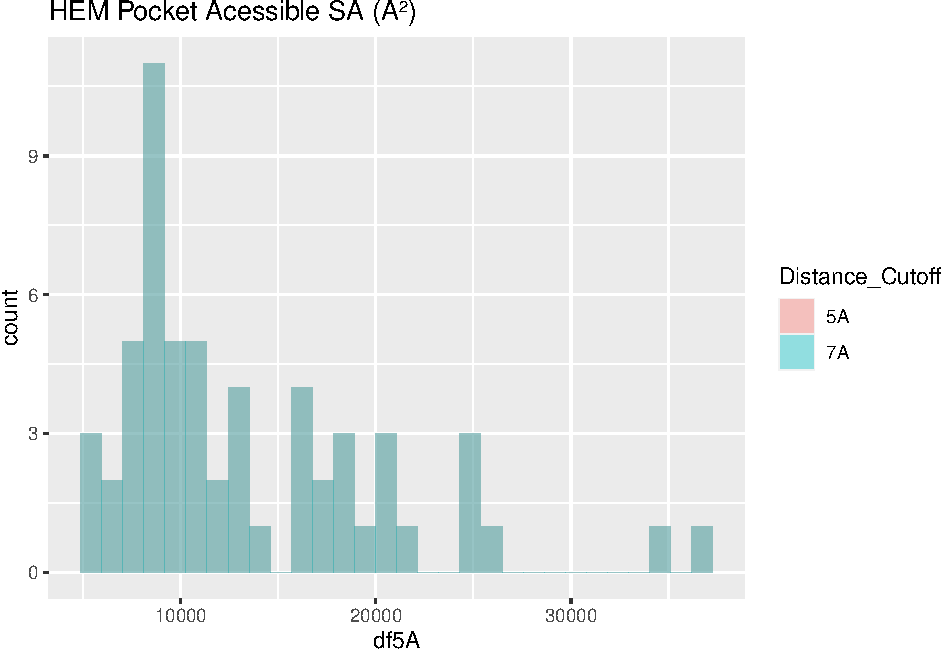
\includegraphics{_main_files/figure-latex/HEM-Pocket-AccessibleSA-1.pdf}
\caption{\label{fig:HEM-Pocket-AccessibleSA}HEM: Pocket Accessible Surface Area}
\end{figure}

\begin{figure}
\centering
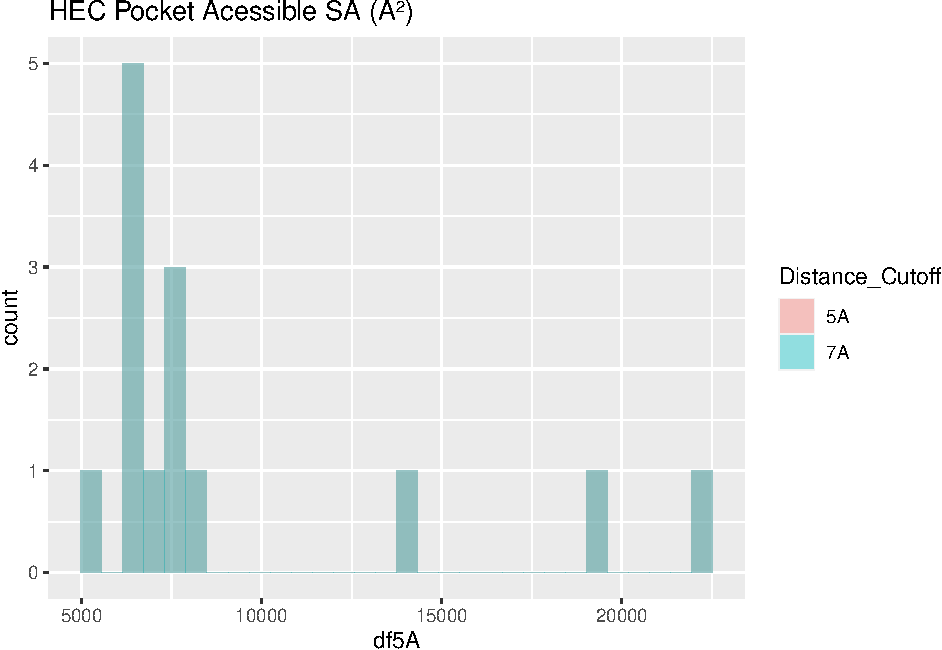
\includegraphics{_main_files/figure-latex/HEC-Pocket-AccessibleSA-1.pdf}
\caption{\label{fig:HEC-Pocket-AccessibleSA}HEC: Pocket Accessible Surface Area}
\end{figure}

\begin{figure}
\centering
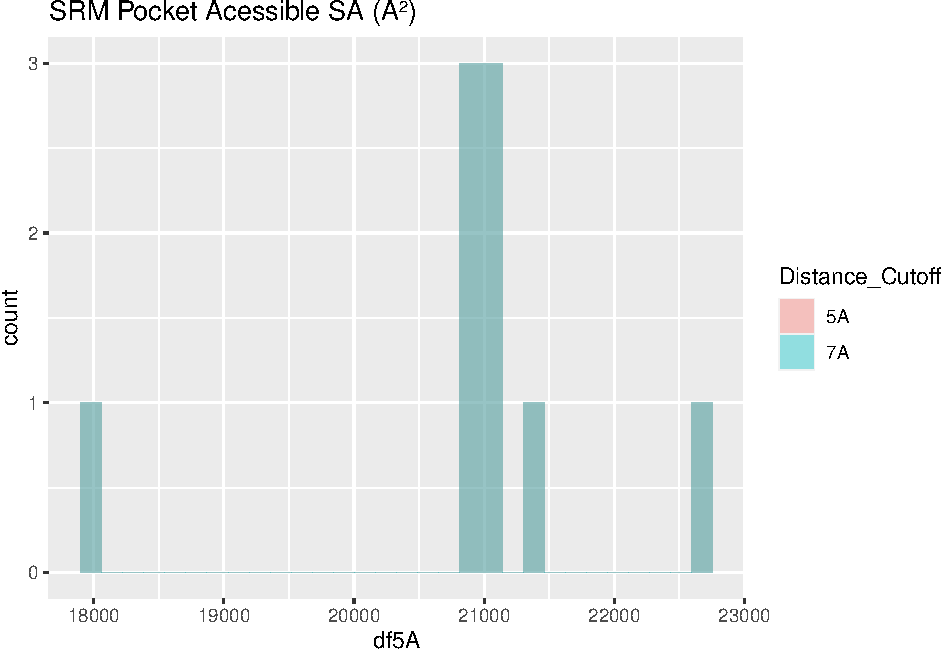
\includegraphics{_main_files/figure-latex/SRM-Pocket-AccessibleSA-1.pdf}
\caption{\label{fig:SRM-Pocket-AccessibleSA}SRM: Pocket Accessible Surface Area}
\end{figure}

\begin{figure}
\centering
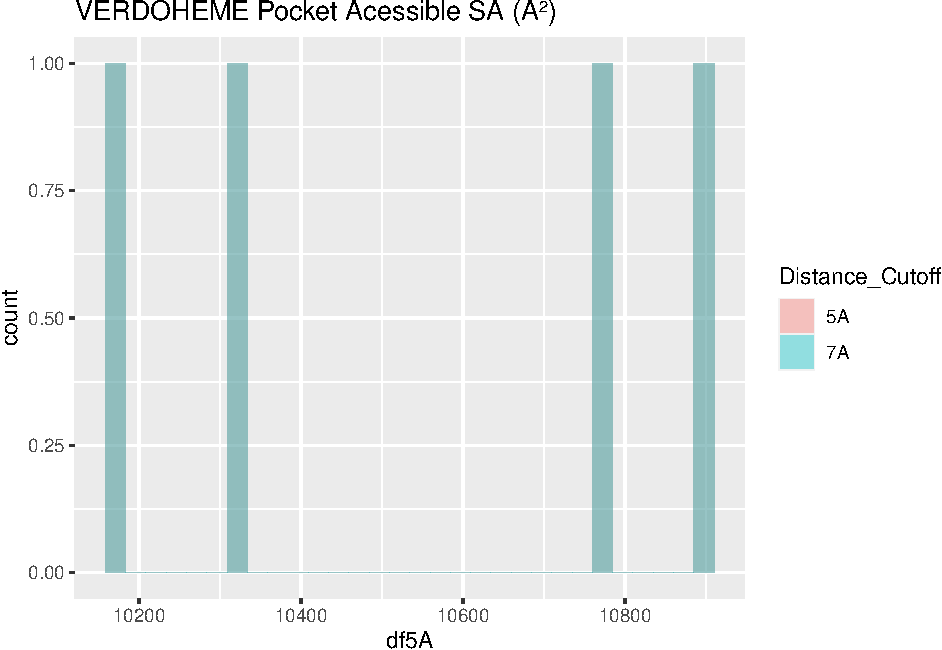
\includegraphics{_main_files/figure-latex/VERDOHEME-Pocket-AccessibleSA-1.pdf}
\caption{\label{fig:VERDOHEME-Pocket-AccessibleSA}VERDOHEME: Pocket Accessible Surface Area}
\end{figure}

\hypertarget{figs-planarAll}{%
\section{All Planar Angles}\label{figs-planarAll}}

\begin{figure}
\centering
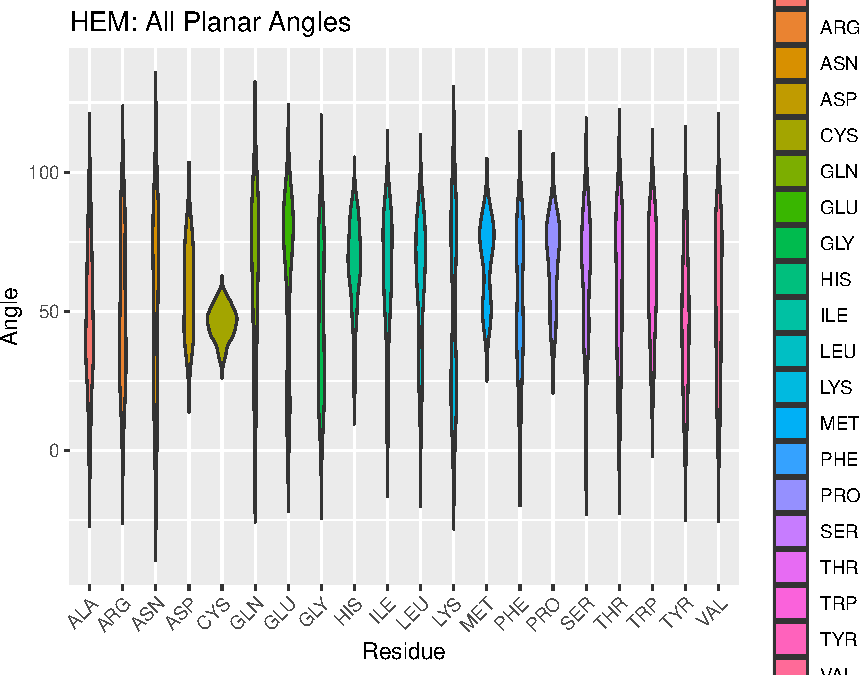
\includegraphics{_main_files/figure-latex/HEM-planarAll-1.pdf}
\caption{\label{fig:HEM-planarAll}HEM: All Planar Angles}
\end{figure}

\begin{figure}
\centering
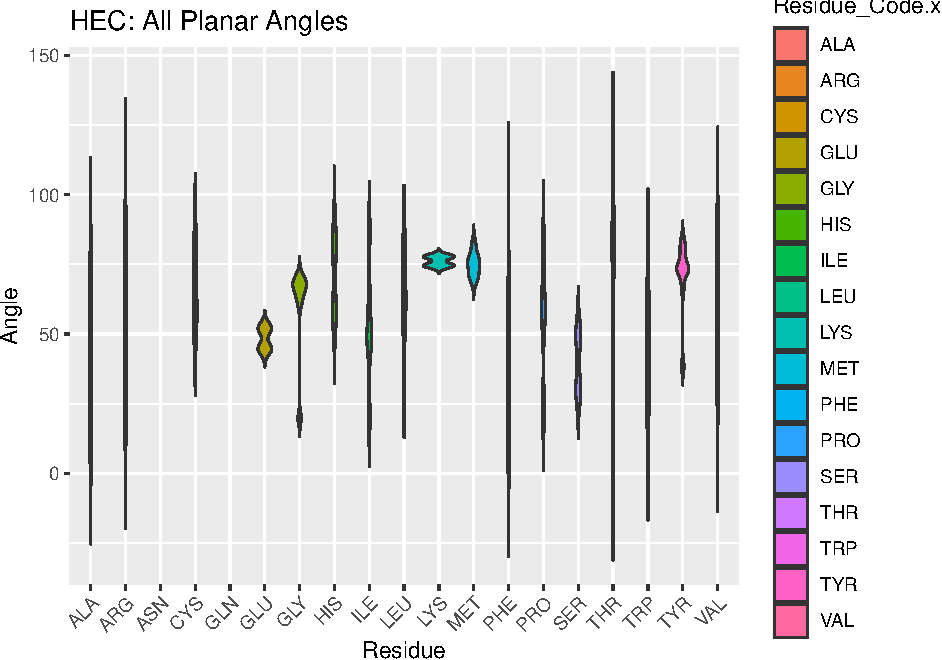
\includegraphics{_main_files/figure-latex/HEC-planarAll-1.pdf}
\caption{\label{fig:HEC-planarAll}HEC: All Planar Angles}
\end{figure}

\begin{figure}
\centering
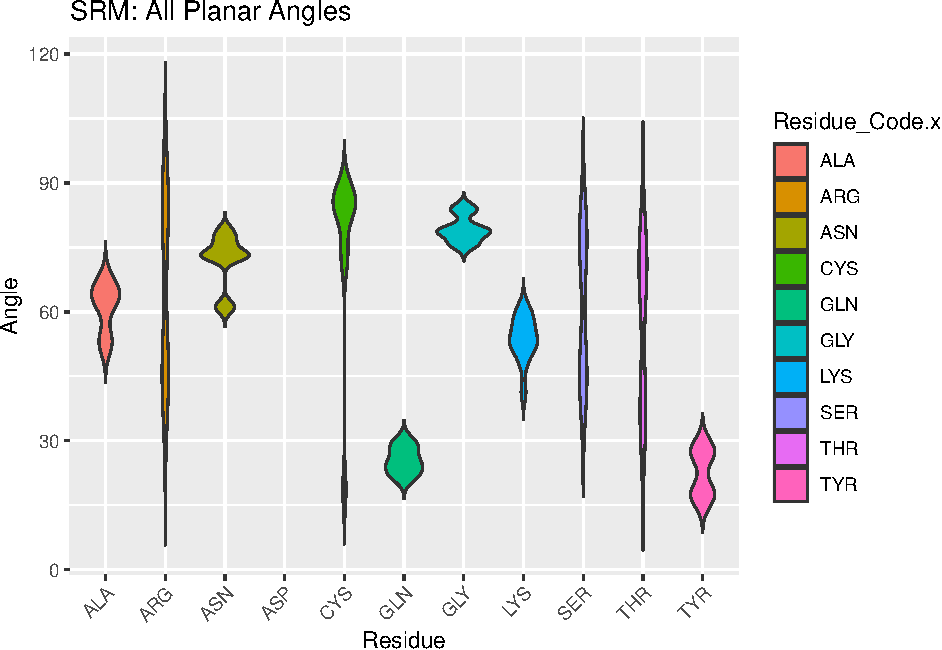
\includegraphics{_main_files/figure-latex/SRM-planarAll-1.pdf}
\caption{\label{fig:SRM-planarAll}SRM: All Planar Angles}
\end{figure}

\begin{figure}
\centering
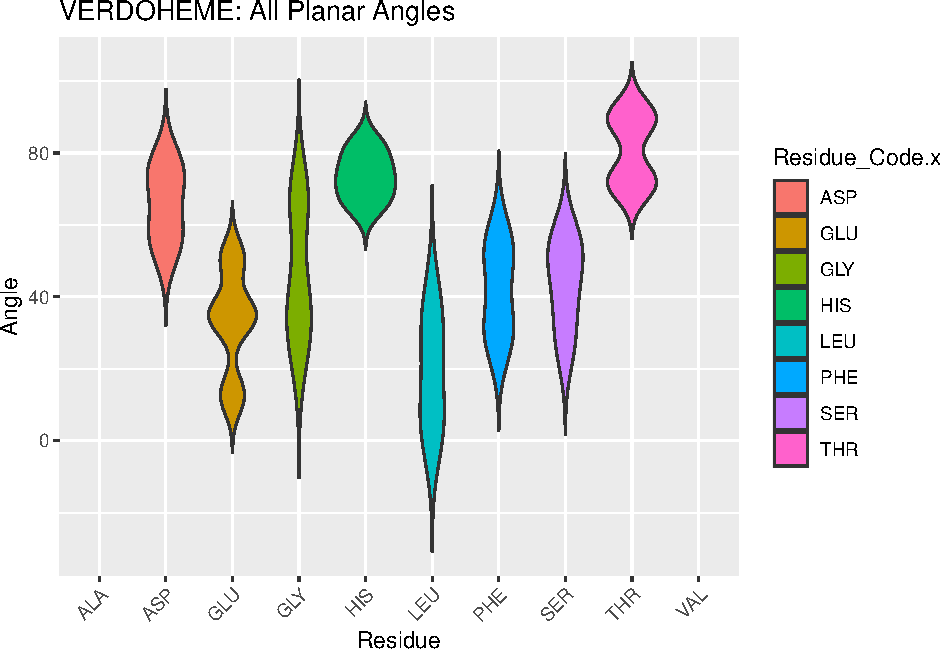
\includegraphics{_main_files/figure-latex/VERDOHEME-planarAll-1.pdf}
\caption{\label{fig:VERDOHEME-planarAll}VERDOHEME: All Planar Angles}
\end{figure}

\hypertarget{figs-planarClosest}{%
\section{Planar Angles of Closest Residues}\label{figs-planarClosest}}

\begin{figure}
\centering
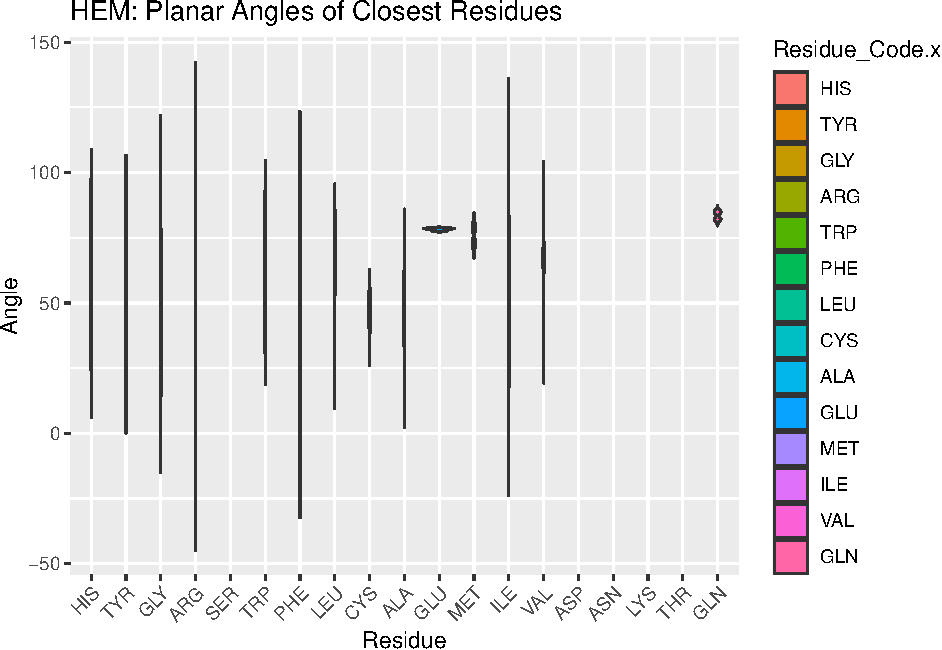
\includegraphics{_main_files/figure-latex/HEM-planarClosest-1.pdf}
\caption{\label{fig:HEM-planarClosest}HEM: Planar Angles of Closest Residues}
\end{figure}

\begin{figure}
\centering
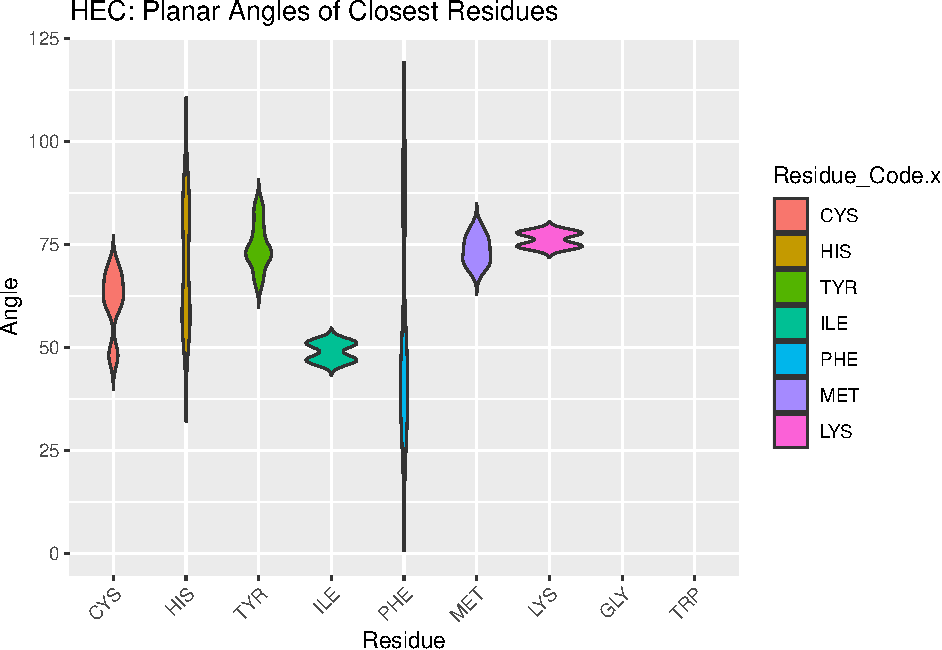
\includegraphics{_main_files/figure-latex/HEC-planarClosest-1.pdf}
\caption{\label{fig:HEC-planarClosest}HEC: Planar Angles of Closest Residues}
\end{figure}

\begin{figure}
\centering
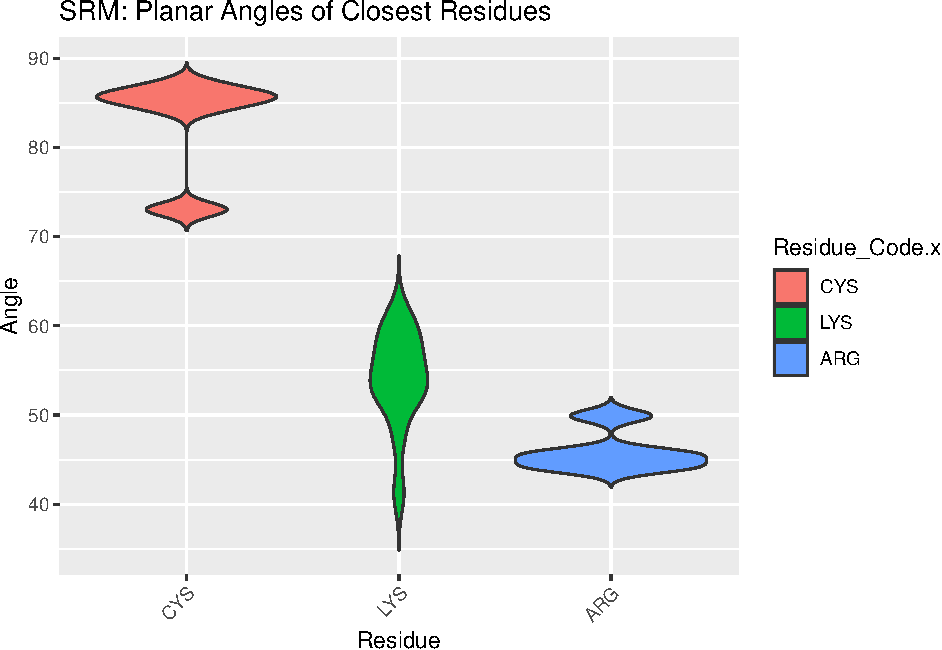
\includegraphics{_main_files/figure-latex/SRM-planarClosest-1.pdf}
\caption{\label{fig:SRM-planarClosest}SRM: Planar Angles of Closest Residues}
\end{figure}

\begin{figure}
\centering
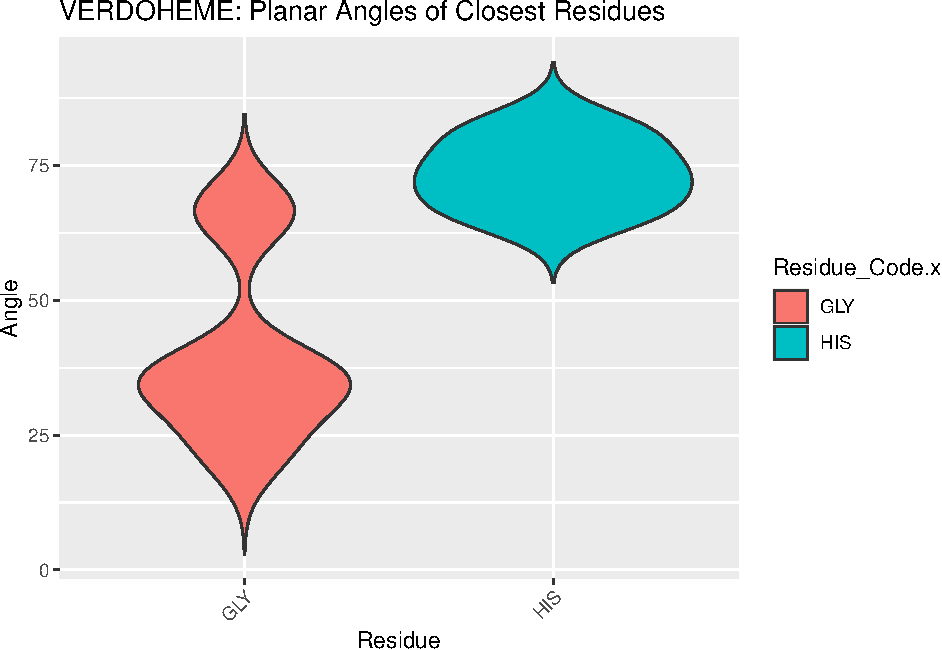
\includegraphics{_main_files/figure-latex/VERDOHEME-planarClosest-1.pdf}
\caption{\label{fig:VERDOHEME-planarClosest}VERDOHEME: Planar Angles of Closest Residues}
\end{figure}

\hypertarget{figs-cabAll}{%
\section{All CA-CB-Fe Angles}\label{figs-cabAll}}

\begin{figure}
\centering
\includegraphics{_main_files/figure-latex/HEM-cab-All-1.pdf}
\caption{\label{fig:HEM-cab-All}HEM: All CA-CB-Fe Angles}
\end{figure}

\begin{figure}
\centering
\includegraphics{_main_files/figure-latex/HEC-cab-All-1.pdf}
\caption{\label{fig:HEC-cab-All}HEC: All CA-CB-Fe Angles}
\end{figure}

\begin{figure}
\centering
\includegraphics{_main_files/figure-latex/SRM-cab-All-1.pdf}
\caption{\label{fig:SRM-cab-All}SRM: All CA-CB-Fe Angles}
\end{figure}

\begin{figure}
\centering
\includegraphics{_main_files/figure-latex/VERDOHEME-cab-All-1.pdf}
\caption{\label{fig:VERDOHEME-cab-All}VERDOHEME: All CA-CB-Fe Angles}
\end{figure}

\hypertarget{figs-cabClosest}{%
\section{CA-CB-Fe Angles of Closest Residues}\label{figs-cabClosest}}

\begin{figure}
\centering
\includegraphics{_main_files/figure-latex/HEM-cabClosest-1.pdf}
\caption{\label{fig:HEM-cabClosest}HEM: CACBFe Angles of Closest Residues}
\end{figure}

\begin{figure}
\centering
\includegraphics{_main_files/figure-latex/HEC-cabClosest-1.pdf}
\caption{\label{fig:HEC-cabClosest}HEC: CACBFe Angles of Closest Residues}
\end{figure}

\begin{figure}
\centering
\includegraphics{_main_files/figure-latex/SRM-cabClosest-1.pdf}
\caption{\label{fig:SRM-cabClosest}SRM: CACBFe Angles of Closest Residues}
\end{figure}

\begin{figure}
\centering
\includegraphics{_main_files/figure-latex/VERDOHEME-cabClosest-1.pdf}
\caption{\label{fig:VERDOHEME-cabClosest}VERDOHEME: CACBFe Angles of Closest Residues}
\end{figure}

\hypertarget{a-tables}{%
\chapter{Tables}\label{a-tables}}

\minitoc

\hypertarget{molOrgSec}{%
\section{Molecule Names and Source Organisms}\label{molOrgSec}}

\begin{longtabu} to \linewidth {>{\raggedright}X>{\raggedright}X>{\raggedright}X}
\caption{\label{tab:HEM-molOrg}HEM: Molecules and Source Organisms}\\
\toprule
\rotatebox{45}{PDB\_ID} & \rotatebox{45}{Molecule\_Name} & \rotatebox{45}{Source\_Organism}\\
\midrule
\endfirsthead
\caption[]{\label{tab:HEM-molOrg}HEM: Molecules and Source Organisms \textit{(continued)}}\\
\toprule
\rotatebox{45}{PDB\_ID} & \rotatebox{45}{Molecule\_Name} & \rotatebox{45}{Source\_Organism}\\
\midrule
\endhead

\endfoot
\bottomrule
\endlastfoot
\cellcolor{gray!6}{1B2V} & \cellcolor{gray!6}{PROTEIN (HEME-BINDING PROTEIN A);} & \cellcolor{gray!6}{SERRATIA MARCESCENS;}\\
1B5M & CYTOCHROME B5; & RATTUS NORVEGICUS;\\
\cellcolor{gray!6}{1DK0} & \cellcolor{gray!6}{HEME-BINDING PROTEIN A;} & \cellcolor{gray!6}{SERRATIA MARCESCENS;}\\
1DKH & HEME-BINDING PROTEIN A; & SERRATIA MARCESCENS;\\
\cellcolor{gray!6}{1ICC} & \cellcolor{gray!6}{CYTOCHROME B5 OUTER MITOCHONDRIAL MEMBRANE} & \cellcolor{gray!6}{RATTUS NORVEGICUS;}\\
\addlinespace
1IPH & CATALASE HPII; & ESCHERICHIA COLI;\\
\cellcolor{gray!6}{1N45} & \cellcolor{gray!6}{HEME OXYGENASE 1;} & \cellcolor{gray!6}{HOMO SAPIENS;}\\
1P3T & HEME OXYGENASE 1; & NEISSERIA MENINGITIDIS;\\
\cellcolor{gray!6}{1QHU} & \cellcolor{gray!6}{PROTEIN (HEMOPEXIN);} & \cellcolor{gray!6}{ORYCTOLAGUS CUNICULUS;}\\
1QJS & HEMOPEXIN; & ORYCTOLAGUS CUNICULUS;\\
\addlinespace
\cellcolor{gray!6}{1SI8} & \cellcolor{gray!6}{CATALASE;} & \cellcolor{gray!6}{ENTEROCOCCUS FAECALIS;}\\
1SY2 & NITROPHORIN 4; & RHODNIUS PROLIXUS;\\
\cellcolor{gray!6}{1U9U} & \cellcolor{gray!6}{CYTOCHROME B5;} & \cellcolor{gray!6}{BOS TAURUS;}\\
1VGI & HEME OXYGENASE 1; & RATTUS NORVEGICUS;\\
\cellcolor{gray!6}{1ZVI} & \cellcolor{gray!6}{NITRIC-OXIDE SYNTHASE, BRAIN;} & \cellcolor{gray!6}{RATTUS NORVEGICUS;}\\
\addlinespace
2BHJ & NITRIC OXIDE SYNTHASE; & MUS MUSCULUS;\\
\cellcolor{gray!6}{2CJ0} & \cellcolor{gray!6}{CHLOROPEROXIDASE;} & \cellcolor{gray!6}{CALDARIOMYCES FUMAGO;}\\
2CN4 & HEMOPHORE HASA; & SERRATIA MARCESCENS;\\
\cellcolor{gray!6}{2CPO} & \cellcolor{gray!6}{CHLOROPEROXIDASE;} & \cellcolor{gray!6}{LEPTOXYPHIUM FUMAGO;}\\
2E2Y & MYOGLOBIN; & PHYSETER CATODON;\\
\addlinespace
\cellcolor{gray!6}{2FC2} & \cellcolor{gray!6}{NITRIC OXIDE SYNTHASE;} & \cellcolor{gray!6}{BACILLUS SUBTILIS;}\\
2IIZ & MELANIN BIOSYNTHESIS PROTEIN TYRA, PUTATIVE; & SHEWANELLA ONEIDENSIS;\\
\cellcolor{gray!6}{2IPS} & \cellcolor{gray!6}{LACTOPEROXIDASE;} & \cellcolor{gray!6}{BOS TAURUS;}\\
2J0P & HEMIN TRANSPORT PROTEIN HEMS; & YERSINIA ENTEROCOLITICA;\\
\cellcolor{gray!6}{2J18} & \cellcolor{gray!6}{CHLOROPEROXIDASE;} & \cellcolor{gray!6}{CALDARIOMYCES FUMAGO;}\\
\addlinespace
2O6P & IRON-REGULATED SURFACE DETERMINANT PROTEIN C; & STAPHYLOCOCCUS AUREUS SUBSP. AUREUS;\\
\cellcolor{gray!6}{2Q6N} & \cellcolor{gray!6}{CYTOCHROME P450 2B4;} & \cellcolor{gray!6}{ORYCTOLAGUS CUNICULUS;}\\
2R7A & BACTERIAL HEME BINDING PROTEIN; & SHIGELLA DYSENTERIAE;\\
\cellcolor{gray!6}{2SPL} & \cellcolor{gray!6}{MYOGLOBIN;} & \cellcolor{gray!6}{PHYSETER CATODON;}\\
2VEB & PROTOGLOBIN; & METHANOSARCINA ACETIVORANS;\\
\addlinespace
\cellcolor{gray!6}{3HX9} & \cellcolor{gray!6}{PROTEIN RV3592;} & \cellcolor{gray!6}{MYCOBACTERIUM TUBERCULOSIS;}\\
3MVF & NITROPHORIN-4; & RHODNIUS PROLIXUS;\\
\cellcolor{gray!6}{3QZN} & \cellcolor{gray!6}{IRON-REGULATED SURFACE DETERMINANT PROTEIN A;} & \cellcolor{gray!6}{STAPHYLOCOCCUS AUREUS SUBSP. AUREUS;}\\
3QZZ & METHANOSARCINA ACETIVORANS PROTOGLOBIN; & METHANOSARCINA ACETIVORANS;\\
\cellcolor{gray!6}{3SIK} & \cellcolor{gray!6}{CONSERVED DOMAIN PROTEIN;} & \cellcolor{gray!6}{BACILLUS ANTHRACIS;}\\
\addlinespace
3TGC & NITROPHORIN-4; & RHODNIUS PROLIXUS;\\
\cellcolor{gray!6}{3VP5} & \cellcolor{gray!6}{TRANSCRIPTIONAL REGULATOR;} & \cellcolor{gray!6}{LACTOCOCCUS LACTIS;}\\
3ZJS & PROTOGLOBIN; & METHANOSARCINA ACETIVORANS;\\
\cellcolor{gray!6}{4B8N} & \cellcolor{gray!6}{CYTOCHROME B5-HOST ORIGIN;} & \cellcolor{gray!6}{OSTREOCOCCUS TAURI VIRUS 2;}\\
4CAT & CATALASE; & PENICILLIUM JANTHINELLUM;\\
\addlinespace
\cellcolor{gray!6}{4CDP} & \cellcolor{gray!6}{PUTATIVE HEME/HEMOGLOBIN TRANSPORT PROTEIN;} & \cellcolor{gray!6}{ESCHERICHIA COLI;}\\
4I3Q & CYTOCHROME P450 3A4; & HOMO SAPIENS;\\
\cellcolor{gray!6}{4JET} & \cellcolor{gray!6}{HEMOPHORE HASA;} & \cellcolor{gray!6}{YERSINIA PESTIS;}\\
4MF9 & HEMIN DEGRADING FACTOR; & PSEUDOMONAS AERUGINOSA;\\
\cellcolor{gray!6}{4MYP} & \cellcolor{gray!6}{IRON-REGULATED SURFACE DETERMINANT PROTEIN A;} & \cellcolor{gray!6}{LISTERIA MONOCYTOGENES;}\\
\addlinespace
4NL5 & HEME-DEGRADING MONOOXYGENASE HMOB; & MYCOBACTERIUM TUBERCULOSIS;\\
\cellcolor{gray!6}{4UZV} & \cellcolor{gray!6}{HEMOGLOBIN;} & \cellcolor{gray!6}{THERMOBIFIDA FUSCA TM51;}\\
4XZD & EXTRACELLULAR HEME ACQUISITION HEMOPHORE HASA; & YERSINIA PSEUDOTUBERCULOSIS IP 32953;\\
\cellcolor{gray!6}{4Y1Q} & \cellcolor{gray!6}{EXTRACELLULAR HEME ACQUISITION HEMOPHORE HASA;} & \cellcolor{gray!6}{YERSINIA PSEUDOTUBERCULOSIS IP 32953;}\\
5CN5 & MYOGLOBIN; & EQUUS CABALLUS;\\
\addlinespace
\cellcolor{gray!6}{5GJ3} & \cellcolor{gray!6}{PERIPLASMIC BINDING PROTEIN;} & \cellcolor{gray!6}{ROSEIFLEXUS SP. RS-1;}\\
5KZL & HEME OXYGENASE; & LEPTOSPIRA INTERROGANS;\\
\cellcolor{gray!6}{5O1L} & \cellcolor{gray!6}{RUBBER OXYGENASE;} & \cellcolor{gray!6}{STREPTOMYCES SP. (STRAIN K30);}\\
5O1M & RUBBER OXYGENASE; & STREPTOMYCES SP. (STRAIN K30);\\
\cellcolor{gray!6}{5VEU} & \cellcolor{gray!6}{CYTOCHROME P450 3A5;} & \cellcolor{gray!6}{HOMO SAPIENS;}\\
\addlinespace
6A2J & HEME A SYNTHASE; & BACILLUS SUBTILIS (STRAIN 168);\\
\cellcolor{gray!6}{7C74} & \cellcolor{gray!6}{LACTOPEROXIDASE;} & \cellcolor{gray!6}{BOS MUTUS;}\\
7DMR & LACTOPEROXIDASE; & BOS MUTUS;\\*
\end{longtabu}

\begin{longtabu} to \linewidth {>{\raggedright}X>{\raggedright}X>{\raggedright}X}
\caption{\label{tab:HEC-molOrg}HEC: Molecules and Source Organisms}\\
\toprule
\rotatebox{45}{PDB\_ID} & \rotatebox{45}{Molecule\_Name} & \rotatebox{45}{Source\_Organism}\\
\midrule
\endfirsthead
\caption[]{\label{tab:HEC-molOrg}HEC: Molecules and Source Organisms \textit{(continued)}}\\
\toprule
\rotatebox{45}{PDB\_ID} & \rotatebox{45}{Molecule\_Name} & \rotatebox{45}{Source\_Organism}\\
\midrule
\endhead

\endfoot
\bottomrule
\endlastfoot
\cellcolor{gray!6}{1BBH} & \cellcolor{gray!6}{CYTOCHROME C';} & \cellcolor{gray!6}{ALLOCHROMATIUM VINOSUM;}\\
1S56 & HEMOGLOBIN-LIKE PROTEIN HBN; & MYCOBACTERIUM TUBERCULOSIS;\\
\cellcolor{gray!6}{1W2L} & \cellcolor{gray!6}{CYTOCHROME OXIDASE SUBUNIT II;} & \cellcolor{gray!6}{RHODOTHERMUS MARINUS;}\\
2BC5 & SOLUBLE CYTOCHROME B562; & ESCHERICHIA COLI;\\
\cellcolor{gray!6}{2BH5} & \cellcolor{gray!6}{CYTOCHROME C-550;} & \cellcolor{gray!6}{PARACOCCUS VERSUTUS;}\\
\addlinespace
3EAH & NITRIC OXIDE SYNTHASE, ENDOTHELIAL; & HOMO SAPIENS;\\
\cellcolor{gray!6}{3X15} & \cellcolor{gray!6}{CYTOCHROME C552;} & \cellcolor{gray!6}{AQUIFEX AEOLICUS VF5;}\\
5KPF & CYTOCHROME C ISO-1; & SACCHAROMYCES CEREVISIAE;\\
\cellcolor{gray!6}{5LFT} & \cellcolor{gray!6}{CYTOCHROME C ISO-1;} & \cellcolor{gray!6}{SACCHAROMYCES CEREVISIAE;}\\
5T8W & CYC1P; & SACCHAROMYCES CEREVISIAE;\\
\addlinespace
\cellcolor{gray!6}{6VDQ} & \cellcolor{gray!6}{3-METHYL-L-TYROSINE PEROXYGENASE;} & \cellcolor{gray!6}{STREPTOMYCES LAVENDULAE;}\\
6WZA & SOLUBLE CYTOCHROME B562; & ESCHERICHIA COLI;\\
\cellcolor{gray!6}{6XNK} & \cellcolor{gray!6}{CYTOCHROME C;} & \cellcolor{gray!6}{HOMO SAPIENS;}\\*
\end{longtabu}

\begin{longtabu} to \linewidth {>{\raggedright}X>{\raggedright}X>{\raggedright}X}
\caption{\label{tab:SRM-molOrg}SRM: Molecules and Source Organisms}\\
\toprule
\rotatebox{45}{PDB\_ID} & \rotatebox{45}{Molecule\_Name} & \rotatebox{45}{Source\_Organism}\\
\midrule
\endfirsthead
\caption[]{\label{tab:SRM-molOrg}SRM: Molecules and Source Organisms \textit{(continued)}}\\
\toprule
\rotatebox{45}{PDB\_ID} & \rotatebox{45}{Molecule\_Name} & \rotatebox{45}{Source\_Organism}\\
\midrule
\endhead

\endfoot
\bottomrule
\endlastfoot
\cellcolor{gray!6}{1ZJ8} & \cellcolor{gray!6}{PROBABLE FERREDOXIN-DEPENDENT NITRITE REDUCTASE NIRA;} & \cellcolor{gray!6}{MYCOBACTERIUM TUBERCULOSIS;}\\
2AKJ & FERREDOXIN--NITRITE REDUCTASE, CHLOROPLAST; & SPINACIA OLERACEA;\\
\cellcolor{gray!6}{2AOP} & \cellcolor{gray!6}{SULFITE REDUCTASE HEMOPROTEIN;} & \cellcolor{gray!6}{ESCHERICHIA COLI;}\\
3B0G & NITRITE REDUCTASE; & NICOTIANA TABACUM;\\
\cellcolor{gray!6}{3VKP} & \cellcolor{gray!6}{NITRITE REDUCTASE;} & \cellcolor{gray!6}{NICOTIANA TABACUM;}\\
\addlinespace
3VLX & NITRITE REDUCTASE; & NICOTIANA TABACUM;\\
\cellcolor{gray!6}{3VLY} & \cellcolor{gray!6}{NITRITE REDUCTASE;} & \cellcolor{gray!6}{NICOTIANA TABACUM;}\\
3VLZ & NITRITE REDUCTASE; & NICOTIANA TABACUM;\\
\cellcolor{gray!6}{5H8V} & \cellcolor{gray!6}{SULFITE REDUCTASE [FERREDOXIN], CHLOROPLASTIC;} & \cellcolor{gray!6}{ZEA MAYS;}\\*
\end{longtabu}

\begin{longtabu} to \linewidth {>{\raggedright}X>{\raggedright}X>{\raggedright}X}
\caption{\label{tab:VERDOHEME-molOrg}VERDOHEME: Molecules and Source Organisms}\\
\toprule
\rotatebox{45}{PDB\_ID} & \rotatebox{45}{Molecule\_Name} & \rotatebox{45}{Source\_Organism}\\
\midrule
\endfirsthead
\caption[]{\label{tab:VERDOHEME-molOrg}VERDOHEME: Molecules and Source Organisms \textit{(continued)}}\\
\toprule
\rotatebox{45}{PDB\_ID} & \rotatebox{45}{Molecule\_Name} & \rotatebox{45}{Source\_Organism}\\
\midrule
\endhead

\endfoot
\bottomrule
\endlastfoot
\cellcolor{gray!6}{2ZVU} & \cellcolor{gray!6}{HEME OXYGENASE 1;} & \cellcolor{gray!6}{RATTUS NORVEGICUS;}\\
3MOO & HEME OXYGENASE; & CORYNEBACTERIUM DIPHTHERIAE;\\
\cellcolor{gray!6}{1TWN} & \cellcolor{gray!6}{HEME OXYGENASE 1;} & \cellcolor{gray!6}{HOMO SAPIENS;}\\
1TWR & HEME OXYGENASE 1; & HOMO SAPIENS;\\*
\end{longtabu}

\hypertarget{distances}{%
\section{Distances}\label{distances}}

\hypertarget{all-distances-from-heme-fe-to-atoms-of-residues-in-binding-pocket}{%
\subsection{All Distances from Heme Fe to Atoms of Residues in Binding Pocket}\label{all-distances-from-heme-fe-to-atoms-of-residues-in-binding-pocket}}

\begin{longtabu} to \linewidth {>{\raggedright}X>{\raggedright}X>{\raggedright}X>{\raggedleft}X>{\raggedright}X>{\raggedleft}X}
\caption{\label{tab:HEM-t-distancesAll}HEM: All Distances, Atoms to Fe}\\
\toprule
\rotatebox{45}{ } & \rotatebox{45}{PDB\_ID} & \rotatebox{45}{Residue\_Code} & \rotatebox{45}{Residue\_Number} & \rotatebox{45}{Atom} & \rotatebox{45}{Distance}\\
\midrule
\endfirsthead
\caption[]{\label{tab:HEM-t-distancesAll}HEM: All Distances, Atoms to Fe \textit{(continued)}}\\
\toprule
\rotatebox{45}{ } & \rotatebox{45}{PDB\_ID} & \rotatebox{45}{Residue\_Code} & \rotatebox{45}{Residue\_Number} & \rotatebox{45}{Atom} & \rotatebox{45}{Distance}\\
\midrule
\endhead

\endfoot
\bottomrule
\endlastfoot
\cellcolor{gray!6}{1} & \cellcolor{gray!6}{1B2V} & \cellcolor{gray!6}{HIS} & \cellcolor{gray!6}{83} & \cellcolor{gray!6}{ND1} & \cellcolor{gray!6}{4.091840}\\
2 & 1B2V & TYR & 75 & CG & 5.370524\\
\cellcolor{gray!6}{3} & \cellcolor{gray!6}{1B2V} & \cellcolor{gray!6}{VAL} & \cellcolor{gray!6}{37} & \cellcolor{gray!6}{CG2} & \cellcolor{gray!6}{5.119564}\\
4 & 1B2V & HIS & 83 & NE2 & 5.795310\\
\cellcolor{gray!6}{5} & \cellcolor{gray!6}{1B2V} & \cellcolor{gray!6}{VAL} & \cellcolor{gray!6}{37} & \cellcolor{gray!6}{CG1} & \cellcolor{gray!6}{5.302293}\\
\addlinespace
6 & 1B2V & LEU & 77 & CA & 6.357591\\
\cellcolor{gray!6}{7} & \cellcolor{gray!6}{1B2V} & \cellcolor{gray!6}{SER} & \cellcolor{gray!6}{42} & \cellcolor{gray!6}{O} & \cellcolor{gray!6}{6.611193}\\
8 & 1B2V & HIS & 83 & CA & 5.317261\\
\cellcolor{gray!6}{9} & \cellcolor{gray!6}{1B2V} & \cellcolor{gray!6}{LEU} & \cellcolor{gray!6}{77} & \cellcolor{gray!6}{N} & \cellcolor{gray!6}{6.764107}\\
10 & 1B2V & TYR & 75 & CZ & 2.888333\\
\addlinespace
\cellcolor{gray!6}{11} & \cellcolor{gray!6}{1B2V} & \cellcolor{gray!6}{TYR} & \cellcolor{gray!6}{75} & \cellcolor{gray!6}{CE1} & \cellcolor{gray!6}{3.676968}\\
12 & 1B2V & TYR & 75 & CD2 & 4.821397\\
\cellcolor{gray!6}{13} & \cellcolor{gray!6}{1B2V} & \cellcolor{gray!6}{TYR} & \cellcolor{gray!6}{75} & \cellcolor{gray!6}{CD1} & \cellcolor{gray!6}{4.880663}\\
14 & 1B2V & TYR & 75 & CB & 6.798699\\
\cellcolor{gray!6}{15} & \cellcolor{gray!6}{1B2V} & \cellcolor{gray!6}{TYR} & \cellcolor{gray!6}{75} & \cellcolor{gray!6}{CE2} & \cellcolor{gray!6}{3.624167}\\
\addlinespace
16 & 1B2V & HIS & 83 & CE1 & 4.910880\\
\cellcolor{gray!6}{17} & \cellcolor{gray!6}{1B2V} & \cellcolor{gray!6}{HIS} & \cellcolor{gray!6}{32} & \cellcolor{gray!6}{CE1} & \cellcolor{gray!6}{3.237980}\\
18 & 1B2V & HIS & 32 & CD2 & 3.186876\\
\cellcolor{gray!6}{19} & \cellcolor{gray!6}{1B2V} & \cellcolor{gray!6}{HIS} & \cellcolor{gray!6}{32} & \cellcolor{gray!6}{ND1} & \cellcolor{gray!6}{4.330731}\\
20 & 1B2V & HIS & 32 & CB & 5.756445\\
\addlinespace
\cellcolor{gray!6}{21} & \cellcolor{gray!6}{1B2V} & \cellcolor{gray!6}{HIS} & \cellcolor{gray!6}{32} & \cellcolor{gray!6}{O} & \cellcolor{gray!6}{5.953564}\\
22 & 1B2V & HIS & 32 & C & 6.358164\\
\cellcolor{gray!6}{23} & \cellcolor{gray!6}{1B2V} & \cellcolor{gray!6}{MET} & \cellcolor{gray!6}{140} & \cellcolor{gray!6}{CE} & \cellcolor{gray!6}{5.777781}\\
24 & 1B2V & MET & 140 & SD & 6.659910\\
\cellcolor{gray!6}{25} & \cellcolor{gray!6}{1B2V} & \cellcolor{gray!6}{HIS} & \cellcolor{gray!6}{83} & \cellcolor{gray!6}{CB} & \cellcolor{gray!6}{4.758791}\\
\addlinespace
26 & 1B2V & HIS & 32 & CA & 6.565816\\
\cellcolor{gray!6}{27} & \cellcolor{gray!6}{1B2V} & \cellcolor{gray!6}{TYR} & \cellcolor{gray!6}{75} & \cellcolor{gray!6}{OH} & \cellcolor{gray!6}{1.954327}\\
28 & 1B2V & SER & 42 & OG & 5.900798\\
\cellcolor{gray!6}{29} & \cellcolor{gray!6}{1B2V} & \cellcolor{gray!6}{SER} & \cellcolor{gray!6}{42} & \cellcolor{gray!6}{CB} & \cellcolor{gray!6}{6.636304}\\
30 & 1B2V & HIS & 32 & CG & 4.355931\\
\addlinespace
\cellcolor{gray!6}{31} & \cellcolor{gray!6}{1B2V} & \cellcolor{gray!6}{LEU} & \cellcolor{gray!6}{77} & \cellcolor{gray!6}{O} & \cellcolor{gray!6}{6.769296}\\
32 & 1B2V & TYR & 137 & CE1 & 6.096698\\
\cellcolor{gray!6}{33} & \cellcolor{gray!6}{1B2V} & \cellcolor{gray!6}{SER} & \cellcolor{gray!6}{42} & \cellcolor{gray!6}{CA} & \cellcolor{gray!6}{6.625250}\\
34 & 1B2V & TYR & 137 & CD1 & 6.368337\\
\cellcolor{gray!6}{35} & \cellcolor{gray!6}{1B2V} & \cellcolor{gray!6}{HIS} & \cellcolor{gray!6}{83} & \cellcolor{gray!6}{CG} & \cellcolor{gray!6}{4.725560}\\
\addlinespace
36 & 1B2V & HIS & 83 & O & 5.883823\\
\cellcolor{gray!6}{37} & \cellcolor{gray!6}{1B2V} & \cellcolor{gray!6}{HIS} & \cellcolor{gray!6}{83} & \cellcolor{gray!6}{C} & \cellcolor{gray!6}{5.884565}\\
38 & 1B2V & ASN & 41 & O & 6.894251\\
\cellcolor{gray!6}{39} & \cellcolor{gray!6}{1B2V} & \cellcolor{gray!6}{HIS} & \cellcolor{gray!6}{83} & \cellcolor{gray!6}{N} & \cellcolor{gray!6}{6.545924}\\
40 & 1B2V & VAL & 37 & CB & 5.853806\\
\addlinespace
\cellcolor{gray!6}{41} & \cellcolor{gray!6}{1B2V} & \cellcolor{gray!6}{THR} & \cellcolor{gray!6}{84} & \cellcolor{gray!6}{N} & \cellcolor{gray!6}{6.798527}\\
42 & 1B2V & HIS & 83 & CD2 & 5.752036\\
\cellcolor{gray!6}{43} & \cellcolor{gray!6}{1B2V} & \cellcolor{gray!6}{HIS} & \cellcolor{gray!6}{32} & \cellcolor{gray!6}{NE2} & \cellcolor{gray!6}{2.263051}\\
44 & 1B2V & LEU & 77 & CD1 & 5.828324\\
\cellcolor{gray!6}{45} & \cellcolor{gray!6}{1B5M} & \cellcolor{gray!6}{HIS} & \cellcolor{gray!6}{63} & \cellcolor{gray!6}{NE2} & \cellcolor{gray!6}{1.819890}\\
\addlinespace
46 & 1B5M & HIS & 63 & CE1 & 3.023255\\
\cellcolor{gray!6}{47} & \cellcolor{gray!6}{1B5M} & \cellcolor{gray!6}{HIS} & \cellcolor{gray!6}{63} & \cellcolor{gray!6}{CD2} & \cellcolor{gray!6}{2.588060}\\
48 & 1B5M & HIS & 63 & ND1 & 4.027399\\
\cellcolor{gray!6}{49} & \cellcolor{gray!6}{1B5M} & \cellcolor{gray!6}{HIS} & \cellcolor{gray!6}{63} & \cellcolor{gray!6}{CG} & \cellcolor{gray!6}{3.837789}\\
50 & 1B5M & HIS & 63 & CB & 5.198178\\
\addlinespace
\cellcolor{gray!6}{51} & \cellcolor{gray!6}{1B5M} & \cellcolor{gray!6}{PRO} & \cellcolor{gray!6}{40} & \cellcolor{gray!6}{CD} & \cellcolor{gray!6}{5.362624}\\
52 & 1B5M & PHE & 35 & CZ & 5.731102\\
\cellcolor{gray!6}{53} & \cellcolor{gray!6}{1B5M} & \cellcolor{gray!6}{HIS} & \cellcolor{gray!6}{63} & \cellcolor{gray!6}{CA} & \cellcolor{gray!6}{6.222160}\\
54 & 1B5M & HIS & 63 & N & 6.979191\\
\cellcolor{gray!6}{55} & \cellcolor{gray!6}{1B5M} & \cellcolor{gray!6}{GLY} & \cellcolor{gray!6}{62} & \cellcolor{gray!6}{O} & \cellcolor{gray!6}{6.365897}\\
\addlinespace
56 & 1B5M & PRO & 40 & CG & 6.038149\\
\cellcolor{gray!6}{57} & \cellcolor{gray!6}{1B5M} & \cellcolor{gray!6}{VAL} & \cellcolor{gray!6}{61} & \cellcolor{gray!6}{CG2} & \cellcolor{gray!6}{6.762820}\\
58 & 1B5M & VAL & 61 & CG1 & 5.208622\\
\cellcolor{gray!6}{59} & \cellcolor{gray!6}{1B5M} & \cellcolor{gray!6}{VAL} & \cellcolor{gray!6}{61} & \cellcolor{gray!6}{CB} & \cellcolor{gray!6}{6.253291}\\
60 & 1B5M & PRO & 40 & CB & 6.380659\\
\addlinespace
\cellcolor{gray!6}{61} & \cellcolor{gray!6}{1B5M} & \cellcolor{gray!6}{HIS} & \cellcolor{gray!6}{39} & \cellcolor{gray!6}{NE2} & \cellcolor{gray!6}{1.918499}\\
62 & 1B5M & LEU & 46 & CD2 & 5.100407\\
\cellcolor{gray!6}{63} & \cellcolor{gray!6}{1B5M} & \cellcolor{gray!6}{LEU} & \cellcolor{gray!6}{46} & \cellcolor{gray!6}{CD1} & \cellcolor{gray!6}{6.238688}\\
64 & 1B5M & LEU & 46 & CG & 6.207115\\
\cellcolor{gray!6}{65} & \cellcolor{gray!6}{1B5M} & \cellcolor{gray!6}{PRO} & \cellcolor{gray!6}{40} & \cellcolor{gray!6}{C} & \cellcolor{gray!6}{6.098869}\\
\addlinespace
66 & 1B5M & VAL & 45 & CG1 & 5.846522\\
\cellcolor{gray!6}{67} & \cellcolor{gray!6}{1B5M} & \cellcolor{gray!6}{HIS} & \cellcolor{gray!6}{39} & \cellcolor{gray!6}{CG} & \cellcolor{gray!6}{4.056245}\\
68 & 1B5M & PRO & 40 & CA & 6.434682\\
\cellcolor{gray!6}{69} & \cellcolor{gray!6}{1B5M} & \cellcolor{gray!6}{PHE} & \cellcolor{gray!6}{58} & \cellcolor{gray!6}{CZ} & \cellcolor{gray!6}{6.351848}\\
70 & 1B5M & PHE & 58 & CE2 & 5.187940\\
\addlinespace
\cellcolor{gray!6}{71} & \cellcolor{gray!6}{1B5M} & \cellcolor{gray!6}{PHE} & \cellcolor{gray!6}{58} & \cellcolor{gray!6}{CD2} & \cellcolor{gray!6}{5.070064}\\
72 & 1B5M & PRO & 40 & N & 5.880309\\
\cellcolor{gray!6}{73} & \cellcolor{gray!6}{1B5M} & \cellcolor{gray!6}{PHE} & \cellcolor{gray!6}{58} & \cellcolor{gray!6}{CG} & \cellcolor{gray!6}{6.133869}\\
74 & 1B5M & PHE & 58 & CB & 6.546370\\
\cellcolor{gray!6}{75} & \cellcolor{gray!6}{1B5M} & \cellcolor{gray!6}{PHE} & \cellcolor{gray!6}{58} & \cellcolor{gray!6}{O} & \cellcolor{gray!6}{6.794383}\\
\addlinespace
76 & 1B5M & PHE & 58 & CA & 6.591026\\
\cellcolor{gray!6}{77} & \cellcolor{gray!6}{1B5M} & \cellcolor{gray!6}{HIS} & \cellcolor{gray!6}{39} & \cellcolor{gray!6}{CE1} & \cellcolor{gray!6}{2.767199}\\
78 & 1B5M & GLY & 42 & O & 6.731713\\
\cellcolor{gray!6}{79} & \cellcolor{gray!6}{1B5M} & \cellcolor{gray!6}{GLY} & \cellcolor{gray!6}{41} & \cellcolor{gray!6}{O} & \cellcolor{gray!6}{5.998395}\\
80 & 1B5M & GLY & 41 & C & 5.685211\\
\addlinespace
\cellcolor{gray!6}{81} & \cellcolor{gray!6}{1B5M} & \cellcolor{gray!6}{GLY} & \cellcolor{gray!6}{41} & \cellcolor{gray!6}{CA} & \cellcolor{gray!6}{4.980319}\\
82 & 1B5M & GLY & 41 & N & 4.888585\\
\cellcolor{gray!6}{83} & \cellcolor{gray!6}{1B5M} & \cellcolor{gray!6}{HIS} & \cellcolor{gray!6}{39} & \cellcolor{gray!6}{ND1} & \cellcolor{gray!6}{3.934694}\\
84 & 1B5M & PHE & 35 & CE2 & 5.325081\\
\cellcolor{gray!6}{85} & \cellcolor{gray!6}{1B5M} & \cellcolor{gray!6}{HIS} & \cellcolor{gray!6}{39} & \cellcolor{gray!6}{CD2} & \cellcolor{gray!6}{3.022098}\\
\addlinespace
86 & 1B5M & HIS & 39 & CB & 5.471773\\
\cellcolor{gray!6}{87} & \cellcolor{gray!6}{1B5M} & \cellcolor{gray!6}{HIS} & \cellcolor{gray!6}{39} & \cellcolor{gray!6}{O} & \cellcolor{gray!6}{6.809826}\\
88 & 1B5M & HIS & 39 & C & 6.158780\\
\cellcolor{gray!6}{89} & \cellcolor{gray!6}{1B5M} & \cellcolor{gray!6}{GLY} & \cellcolor{gray!6}{42} & \cellcolor{gray!6}{N} & \cellcolor{gray!6}{6.336121}\\
90 & 1B5M & PHE & 35 & CD2 & 6.489161\\
\addlinespace
\cellcolor{gray!6}{91} & \cellcolor{gray!6}{1B5M} & \cellcolor{gray!6}{ALA} & \cellcolor{gray!6}{67} & \cellcolor{gray!6}{CB} & \cellcolor{gray!6}{5.797296}\\
92 & 1B5M & HIS & 39 & CA & 5.972168\\
\cellcolor{gray!6}{93} & \cellcolor{gray!6}{1DK0} & \cellcolor{gray!6}{HIS} & \cellcolor{gray!6}{32} & \cellcolor{gray!6}{CE1} & \cellcolor{gray!6}{3.097081}\\
94 & 1DK0 & TYR & 75 & CD1 & 4.870310\\
\cellcolor{gray!6}{95} & \cellcolor{gray!6}{1DK0} & \cellcolor{gray!6}{TYR} & \cellcolor{gray!6}{75} & \cellcolor{gray!6}{CG} & \cellcolor{gray!6}{5.439675}\\
\addlinespace
96 & 1DK0 & TYR & 75 & CB & 6.855877\\
\cellcolor{gray!6}{97} & \cellcolor{gray!6}{1DK0} & \cellcolor{gray!6}{HIS} & \cellcolor{gray!6}{32} & \cellcolor{gray!6}{CD2} & \cellcolor{gray!6}{3.087544}\\
98 & 1DK0 & TYR & 137 & CE1 & 6.058239\\
\cellcolor{gray!6}{99} & \cellcolor{gray!6}{1DK0} & \cellcolor{gray!6}{MET} & \cellcolor{gray!6}{140} & \cellcolor{gray!6}{CE} & \cellcolor{gray!6}{5.680994}\\
100 & 1DK0 & HIS & 32 & ND1 & 4.178511\\
\addlinespace
\cellcolor{gray!6}{101} & \cellcolor{gray!6}{1DK0} & \cellcolor{gray!6}{MET} & \cellcolor{gray!6}{140} & \cellcolor{gray!6}{SD} & \cellcolor{gray!6}{6.690840}\\
102 & 1DK0 & VAL & 37 & CG2 & 5.172684\\
\cellcolor{gray!6}{103} & \cellcolor{gray!6}{1DK0} & \cellcolor{gray!6}{VAL} & \cellcolor{gray!6}{37} & \cellcolor{gray!6}{CG1} & \cellcolor{gray!6}{5.226870}\\
104 & 1DK0 & VAL & 37 & CB & 5.802353\\
\cellcolor{gray!6}{105} & \cellcolor{gray!6}{1DK0} & \cellcolor{gray!6}{HIS} & \cellcolor{gray!6}{32} & \cellcolor{gray!6}{CG} & \cellcolor{gray!6}{4.227248}\\
\addlinespace
106 & 1DK0 & HIS & 32 & CB & 5.635484\\
\cellcolor{gray!6}{107} & \cellcolor{gray!6}{1DK0} & \cellcolor{gray!6}{HIS} & \cellcolor{gray!6}{83} & \cellcolor{gray!6}{NE2} & \cellcolor{gray!6}{5.746185}\\
108 & 1DK0 & HIS & 83 & CD2 & 5.738879\\
\cellcolor{gray!6}{109} & \cellcolor{gray!6}{1DK0} & \cellcolor{gray!6}{HIS} & \cellcolor{gray!6}{83} & \cellcolor{gray!6}{CG} & \cellcolor{gray!6}{4.688593}\\
110 & 1DK0 & SER & 42 & CB & 6.491744\\
\addlinespace
\cellcolor{gray!6}{111} & \cellcolor{gray!6}{1DK0} & \cellcolor{gray!6}{HIS} & \cellcolor{gray!6}{83} & \cellcolor{gray!6}{O} & \cellcolor{gray!6}{5.767033}\\
112 & 1DK0 & TYR & 137 & CD1 & 6.315661\\
\cellcolor{gray!6}{113} & \cellcolor{gray!6}{1DK0} & \cellcolor{gray!6}{HIS} & \cellcolor{gray!6}{83} & \cellcolor{gray!6}{C} & \cellcolor{gray!6}{5.875345}\\
114 & 1DK0 & HIS & 83 & CA & 5.309550\\
\cellcolor{gray!6}{115} & \cellcolor{gray!6}{1DK0} & \cellcolor{gray!6}{HIS} & \cellcolor{gray!6}{83} & \cellcolor{gray!6}{N} & \cellcolor{gray!6}{6.515875}\\
\addlinespace
116 & 1DK0 & HIS & 32 & O & 5.920129\\
\cellcolor{gray!6}{117} & \cellcolor{gray!6}{1DK0} & \cellcolor{gray!6}{THR} & \cellcolor{gray!6}{33} & \cellcolor{gray!6}{N} & \cellcolor{gray!6}{6.991008}\\
118 & 1DK0 & SER & 42 & O & 6.312383\\
\cellcolor{gray!6}{119} & \cellcolor{gray!6}{1DK0} & \cellcolor{gray!6}{SER} & \cellcolor{gray!6}{42} & \cellcolor{gray!6}{C} & \cellcolor{gray!6}{6.937601}\\
120 & 1DK0 & HIS & 32 & CA & 6.464415\\
\addlinespace
\cellcolor{gray!6}{121} & \cellcolor{gray!6}{1DK0} & \cellcolor{gray!6}{THR} & \cellcolor{gray!6}{84} & \cellcolor{gray!6}{N} & \cellcolor{gray!6}{6.799510}\\
122 & 1DK0 & SER & 42 & CA & 6.419147\\
\cellcolor{gray!6}{123} & \cellcolor{gray!6}{1DK0} & \cellcolor{gray!6}{HIS} & \cellcolor{gray!6}{83} & \cellcolor{gray!6}{ND1} & \cellcolor{gray!6}{3.985590}\\
124 & 1DK0 & HIS & 83 & CE1 & 4.767730\\
\cellcolor{gray!6}{125} & \cellcolor{gray!6}{1DK0} & \cellcolor{gray!6}{HIS} & \cellcolor{gray!6}{83} & \cellcolor{gray!6}{CB} & \cellcolor{gray!6}{4.746551}\\
\addlinespace
126 & 1DK0 & LEU & 77 & CD1 & 5.795751\\
\cellcolor{gray!6}{127} & \cellcolor{gray!6}{1DK0} & \cellcolor{gray!6}{HIS} & \cellcolor{gray!6}{32} & \cellcolor{gray!6}{C} & \cellcolor{gray!6}{6.271135}\\
128 & 1DK0 & LEU & 77 & O & 6.856344\\
\cellcolor{gray!6}{129} & \cellcolor{gray!6}{1DK0} & \cellcolor{gray!6}{LEU} & \cellcolor{gray!6}{77} & \cellcolor{gray!6}{CA} & \cellcolor{gray!6}{6.468919}\\
130 & 1DK0 & LEU & 77 & N & 6.888315\\
\addlinespace
\cellcolor{gray!6}{131} & \cellcolor{gray!6}{1DK0} & \cellcolor{gray!6}{ASN} & \cellcolor{gray!6}{41} & \cellcolor{gray!6}{O} & \cellcolor{gray!6}{6.870425}\\
132 & 1DK0 & HIS & 32 & NE2 & 2.123754\\
\cellcolor{gray!6}{133} & \cellcolor{gray!6}{1DK0} & \cellcolor{gray!6}{TYR} & \cellcolor{gray!6}{75} & \cellcolor{gray!6}{OH} & \cellcolor{gray!6}{2.104736}\\
134 & 1DK0 & TYR & 75 & CZ & 3.011905\\
\cellcolor{gray!6}{135} & \cellcolor{gray!6}{1DK0} & \cellcolor{gray!6}{TYR} & \cellcolor{gray!6}{75} & \cellcolor{gray!6}{CE2} & \cellcolor{gray!6}{3.827799}\\
\addlinespace
136 & 1DK0 & TYR & 75 & CE1 & 3.681995\\
\cellcolor{gray!6}{137} & \cellcolor{gray!6}{1DK0} & \cellcolor{gray!6}{TYR} & \cellcolor{gray!6}{75} & \cellcolor{gray!6}{CD2} & \cellcolor{gray!6}{4.982425}\\
138 & 1DKH & HIS & 83 & C & 5.475302\\
\cellcolor{gray!6}{139} & \cellcolor{gray!6}{1DKH} & \cellcolor{gray!6}{HIS} & \cellcolor{gray!6}{32} & \cellcolor{gray!6}{NE2} & \cellcolor{gray!6}{2.724049}\\
140 & 1DKH & VAL & 37 & CG2 & 5.406826\\
\addlinespace
\cellcolor{gray!6}{141} & \cellcolor{gray!6}{1DKH} & \cellcolor{gray!6}{VAL} & \cellcolor{gray!6}{37} & \cellcolor{gray!6}{CG1} & \cellcolor{gray!6}{5.465432}\\
142 & 1DKH & VAL & 37 & CB & 6.056663\\
\cellcolor{gray!6}{143} & \cellcolor{gray!6}{1DKH} & \cellcolor{gray!6}{MET} & \cellcolor{gray!6}{140} & \cellcolor{gray!6}{SD} & \cellcolor{gray!6}{6.766447}\\
144 & 1DKH & HIS & 32 & CD2 & 3.417608\\
\cellcolor{gray!6}{145} & \cellcolor{gray!6}{1DKH} & \cellcolor{gray!6}{LEU} & \cellcolor{gray!6}{77} & \cellcolor{gray!6}{CD1} & \cellcolor{gray!6}{5.235716}\\
\addlinespace
146 & 1DKH & LEU & 77 & CG & 6.605671\\
\cellcolor{gray!6}{147} & \cellcolor{gray!6}{1DKH} & \cellcolor{gray!6}{LEU} & \cellcolor{gray!6}{77} & \cellcolor{gray!6}{CB} & \cellcolor{gray!6}{6.797675}\\
148 & 1DKH & LEU & 77 & O & 6.249675\\
\cellcolor{gray!6}{149} & \cellcolor{gray!6}{1DKH} & \cellcolor{gray!6}{LEU} & \cellcolor{gray!6}{77} & \cellcolor{gray!6}{C} & \cellcolor{gray!6}{6.847101}\\
150 & 1DKH & MET & 140 & CE & 6.272749\\
\addlinespace
\cellcolor{gray!6}{151} & \cellcolor{gray!6}{1DKH} & \cellcolor{gray!6}{HIS} & \cellcolor{gray!6}{32} & \cellcolor{gray!6}{CG} & \cellcolor{gray!6}{4.691025}\\
152 & 1DKH & TYR & 75 & OH & 2.627310\\
\cellcolor{gray!6}{153} & \cellcolor{gray!6}{1DKH} & \cellcolor{gray!6}{TYR} & \cellcolor{gray!6}{75} & \cellcolor{gray!6}{CZ} & \cellcolor{gray!6}{3.786304}\\
154 & 1DKH & TYR & 75 & CE2 & 4.326754\\
\cellcolor{gray!6}{155} & \cellcolor{gray!6}{1DKH} & \cellcolor{gray!6}{TYR} & \cellcolor{gray!6}{75} & \cellcolor{gray!6}{CE1} & \cellcolor{gray!6}{4.788814}\\
\addlinespace
156 & 1DKH & TYR & 75 & CD2 & 5.640713\\
\cellcolor{gray!6}{157} & \cellcolor{gray!6}{1DKH} & \cellcolor{gray!6}{TYR} & \cellcolor{gray!6}{75} & \cellcolor{gray!6}{CD1} & \cellcolor{gray!6}{6.003591}\\
158 & 1DKH & TYR & 137 & CE1 & 6.287721\\
\cellcolor{gray!6}{159} & \cellcolor{gray!6}{1DKH} & \cellcolor{gray!6}{TYR} & \cellcolor{gray!6}{137} & \cellcolor{gray!6}{CD1} & \cellcolor{gray!6}{6.530572}\\
160 & 1DKH & HIS & 32 & O & 6.582967\\
\addlinespace
\cellcolor{gray!6}{161} & \cellcolor{gray!6}{1DKH} & \cellcolor{gray!6}{THR} & \cellcolor{gray!6}{84} & \cellcolor{gray!6}{N} & \cellcolor{gray!6}{6.267175}\\
162 & 1DKH & HIS & 83 & NE2 & 6.220128\\
\cellcolor{gray!6}{163} & \cellcolor{gray!6}{1DKH} & \cellcolor{gray!6}{HIS} & \cellcolor{gray!6}{83} & \cellcolor{gray!6}{CE1} & \cellcolor{gray!6}{5.346327}\\
164 & 1DKH & HIS & 83 & CD2 & 5.826319\\
\cellcolor{gray!6}{165} & \cellcolor{gray!6}{1DKH} & \cellcolor{gray!6}{HIS} & \cellcolor{gray!6}{32} & \cellcolor{gray!6}{CE1} & \cellcolor{gray!6}{3.857511}\\
\addlinespace
166 & 1DKH & HIS & 83 & CG & 4.536138\\
\cellcolor{gray!6}{167} & \cellcolor{gray!6}{1DKH} & \cellcolor{gray!6}{HIS} & \cellcolor{gray!6}{83} & \cellcolor{gray!6}{CB} & \cellcolor{gray!6}{3.988182}\\
168 & 1DKH & HIS & 83 & O & 5.472828\\
\cellcolor{gray!6}{169} & \cellcolor{gray!6}{1DKH} & \cellcolor{gray!6}{HIS} & \cellcolor{gray!6}{32} & \cellcolor{gray!6}{CB} & \cellcolor{gray!6}{5.968356}\\
170 & 1DKH & HIS & 83 & CA & 4.987602\\
\addlinespace
\cellcolor{gray!6}{171} & \cellcolor{gray!6}{1DKH} & \cellcolor{gray!6}{HIS} & \cellcolor{gray!6}{83} & \cellcolor{gray!6}{N} & \cellcolor{gray!6}{6.204508}\\
172 & 1DKH & HIS & 32 & CA & 6.872067\\
\cellcolor{gray!6}{173} & \cellcolor{gray!6}{1DKH} & \cellcolor{gray!6}{TYR} & \cellcolor{gray!6}{75} & \cellcolor{gray!6}{CG} & \cellcolor{gray!6}{6.376320}\\
174 & 1DKH & HIS & 32 & ND1 & 4.892143\\
\cellcolor{gray!6}{175} & \cellcolor{gray!6}{1DKH} & \cellcolor{gray!6}{HIS} & \cellcolor{gray!6}{32} & \cellcolor{gray!6}{C} & \cellcolor{gray!6}{6.888715}\\
\addlinespace
176 & 1DKH & LEU & 77 & CA & 6.337690\\
\cellcolor{gray!6}{177} & \cellcolor{gray!6}{1DKH} & \cellcolor{gray!6}{SER} & \cellcolor{gray!6}{42} & \cellcolor{gray!6}{O} & \cellcolor{gray!6}{6.070312}\\
178 & 1DKH & HIS & 83 & ND1 & 4.180667\\
\cellcolor{gray!6}{179} & \cellcolor{gray!6}{1ICC} & \cellcolor{gray!6}{PHE} & \cellcolor{gray!6}{58} & \cellcolor{gray!6}{CA} & \cellcolor{gray!6}{6.575948}\\
180 & 1ICC & PHE & 58 & CZ & 6.294185\\
\addlinespace
\cellcolor{gray!6}{181} & \cellcolor{gray!6}{1ICC} & \cellcolor{gray!6}{GLY} & \cellcolor{gray!6}{42} & \cellcolor{gray!6}{O} & \cellcolor{gray!6}{6.747263}\\
182 & 1ICC & ALA & 67 & CB & 6.085233\\
\cellcolor{gray!6}{183} & \cellcolor{gray!6}{1ICC} & \cellcolor{gray!6}{GLY} & \cellcolor{gray!6}{41} & \cellcolor{gray!6}{O} & \cellcolor{gray!6}{6.760563}\\
184 & 1ICC & GLY & 41 & C & 6.125467\\
\cellcolor{gray!6}{185} & \cellcolor{gray!6}{1ICC} & \cellcolor{gray!6}{PHE} & \cellcolor{gray!6}{58} & \cellcolor{gray!6}{CG} & \cellcolor{gray!6}{6.377746}\\
\addlinespace
186 & 1ICC & GLY & 41 & N & 4.885432\\
\cellcolor{gray!6}{187} & \cellcolor{gray!6}{1ICC} & \cellcolor{gray!6}{PHE} & \cellcolor{gray!6}{58} & \cellcolor{gray!6}{CE1} & \cellcolor{gray!6}{5.178997}\\
188 & 1ICC & PRO & 40 & CG & 6.377972\\
\cellcolor{gray!6}{189} & \cellcolor{gray!6}{1ICC} & \cellcolor{gray!6}{GLY} & \cellcolor{gray!6}{42} & \cellcolor{gray!6}{N} & \cellcolor{gray!6}{6.567660}\\
190 & 1ICC & HIS & 39 & CG & 4.140159\\
\addlinespace
\cellcolor{gray!6}{191} & \cellcolor{gray!6}{1ICC} & \cellcolor{gray!6}{PRO} & \cellcolor{gray!6}{40} & \cellcolor{gray!6}{C} & \cellcolor{gray!6}{6.026885}\\
192 & 1ICC & PRO & 40 & CA & 6.297086\\
\cellcolor{gray!6}{193} & \cellcolor{gray!6}{1ICC} & \cellcolor{gray!6}{PRO} & \cellcolor{gray!6}{40} & \cellcolor{gray!6}{N} & \cellcolor{gray!6}{5.739901}\\
194 & 1ICC & HIS & 39 & NE2 & 2.123104\\
\cellcolor{gray!6}{195} & \cellcolor{gray!6}{1ICC} & \cellcolor{gray!6}{HIS} & \cellcolor{gray!6}{39} & \cellcolor{gray!6}{CB} & \cellcolor{gray!6}{5.505745}\\
\addlinespace
196 & 1ICC & HIS & 39 & CE1 & 3.226539\\
\cellcolor{gray!6}{197} & \cellcolor{gray!6}{1ICC} & \cellcolor{gray!6}{HIS} & \cellcolor{gray!6}{39} & \cellcolor{gray!6}{CD2} & \cellcolor{gray!6}{2.926974}\\
198 & 1ICC & HIS & 39 & ND1 & 4.243412\\
\cellcolor{gray!6}{199} & \cellcolor{gray!6}{1ICC} & \cellcolor{gray!6}{PHE} & \cellcolor{gray!6}{58} & \cellcolor{gray!6}{CD1} & \cellcolor{gray!6}{5.245447}\\
200 & 1ICC & HIS & 39 & O & 6.677095\\
\addlinespace
\cellcolor{gray!6}{201} & \cellcolor{gray!6}{1ICC} & \cellcolor{gray!6}{HIS} & \cellcolor{gray!6}{39} & \cellcolor{gray!6}{C} & \cellcolor{gray!6}{6.041067}\\
202 & 1ICC & HIS & 39 & CA & 5.995586\\
\cellcolor{gray!6}{203} & \cellcolor{gray!6}{1ICC} & \cellcolor{gray!6}{HIS} & \cellcolor{gray!6}{63} & \cellcolor{gray!6}{NE2} & \cellcolor{gray!6}{2.158759}\\
204 & 1ICC & GLY & 41 & CA & 5.123949\\
\cellcolor{gray!6}{205} & \cellcolor{gray!6}{1ICC} & \cellcolor{gray!6}{HIS} & \cellcolor{gray!6}{63} & \cellcolor{gray!6}{CD2} & \cellcolor{gray!6}{2.978584}\\
\addlinespace
206 & 1ICC & HIS & 63 & ND1 & 4.298568\\
\cellcolor{gray!6}{207} & \cellcolor{gray!6}{1ICC} & \cellcolor{gray!6}{PHE} & \cellcolor{gray!6}{58} & \cellcolor{gray!6}{CB} & \cellcolor{gray!6}{6.924354}\\
208 & 1ICC & HIS & 63 & CG & 4.195708\\
\cellcolor{gray!6}{209} & \cellcolor{gray!6}{1ICC} & \cellcolor{gray!6}{HIS} & \cellcolor{gray!6}{63} & \cellcolor{gray!6}{CB} & \cellcolor{gray!6}{5.559863}\\
210 & 1ICC & HIS & 63 & CA & 6.336951\\
\addlinespace
\cellcolor{gray!6}{211} & \cellcolor{gray!6}{1ICC} & \cellcolor{gray!6}{HIS} & \cellcolor{gray!6}{63} & \cellcolor{gray!6}{N} & \cellcolor{gray!6}{6.820816}\\
212 & 1ICC & VAL & 45 & CG2 & 5.992035\\
\cellcolor{gray!6}{213} & \cellcolor{gray!6}{1ICC} & \cellcolor{gray!6}{VAL} & \cellcolor{gray!6}{61} & \cellcolor{gray!6}{CG2} & \cellcolor{gray!6}{6.129882}\\
214 & 1ICC & VAL & 61 & CG1 & 5.163116\\
\cellcolor{gray!6}{215} & \cellcolor{gray!6}{1ICC} & \cellcolor{gray!6}{VAL} & \cellcolor{gray!6}{61} & \cellcolor{gray!6}{CB} & \cellcolor{gray!6}{5.887227}\\
\addlinespace
216 & 1ICC & PRO & 40 & CD & 5.404471\\
\cellcolor{gray!6}{217} & \cellcolor{gray!6}{1ICC} & \cellcolor{gray!6}{PHE} & \cellcolor{gray!6}{35} & \cellcolor{gray!6}{CZ} & \cellcolor{gray!6}{5.656220}\\
218 & 1ICC & PHE & 35 & CE2 & 5.581214\\
\cellcolor{gray!6}{219} & \cellcolor{gray!6}{1ICC} & \cellcolor{gray!6}{PHE} & \cellcolor{gray!6}{35} & \cellcolor{gray!6}{CE1} & \cellcolor{gray!6}{6.965375}\\
220 & 1ICC & PHE & 35 & CD2 & 6.904462\\
\addlinespace
\cellcolor{gray!6}{221} & \cellcolor{gray!6}{1ICC} & \cellcolor{gray!6}{PHE} & \cellcolor{gray!6}{58} & \cellcolor{gray!6}{O} & \cellcolor{gray!6}{6.678997}\\
222 & 1ICC & PRO & 40 & CB & 6.254107\\
\cellcolor{gray!6}{223} & \cellcolor{gray!6}{1ICC} & \cellcolor{gray!6}{LEU} & \cellcolor{gray!6}{46} & \cellcolor{gray!6}{CD1} & \cellcolor{gray!6}{6.354825}\\
224 & 1ICC & LEU & 46 & CD2 & 5.305231\\
\cellcolor{gray!6}{225} & \cellcolor{gray!6}{1ICC} & \cellcolor{gray!6}{LEU} & \cellcolor{gray!6}{46} & \cellcolor{gray!6}{CG} & \cellcolor{gray!6}{6.164095}\\
\addlinespace
226 & 1ICC & HIS & 63 & CE1 & 3.261015\\
\cellcolor{gray!6}{227} & \cellcolor{gray!6}{1IPH} & \cellcolor{gray!6}{TYR} & \cellcolor{gray!6}{415} & \cellcolor{gray!6}{CD1} & \cellcolor{gray!6}{5.321445}\\
228 & 1IPH & TYR & 415 & CG & 5.753097\\
\cellcolor{gray!6}{229} & \cellcolor{gray!6}{1IPH} & \cellcolor{gray!6}{TYR} & \cellcolor{gray!6}{415} & \cellcolor{gray!6}{CD2} & \cellcolor{gray!6}{5.155005}\\
230 & 1IPH & PHE & 214 & CZ & 4.709378\\
\addlinespace
\cellcolor{gray!6}{231} & \cellcolor{gray!6}{1IPH} & \cellcolor{gray!6}{VAL} & \cellcolor{gray!6}{199} & \cellcolor{gray!6}{CG1} & \cellcolor{gray!6}{5.331401}\\
232 & 1IPH & VAL & 199 & CB & 6.674711\\
\cellcolor{gray!6}{233} & \cellcolor{gray!6}{1IPH} & \cellcolor{gray!6}{VAL} & \cellcolor{gray!6}{199} & \cellcolor{gray!6}{O} & \cellcolor{gray!6}{6.876508}\\
234 & 1IPH & VAL & 127 & CG1 & 6.932478\\
\cellcolor{gray!6}{235} & \cellcolor{gray!6}{1IPH} & \cellcolor{gray!6}{VAL} & \cellcolor{gray!6}{127} & \cellcolor{gray!6}{CB} & \cellcolor{gray!6}{6.007625}\\
\addlinespace
236 & 1IPH & PHE & 214 & CD2 & 6.247230\\
\cellcolor{gray!6}{237} & \cellcolor{gray!6}{1IPH} & \cellcolor{gray!6}{PHE} & \cellcolor{gray!6}{214} & \cellcolor{gray!6}{CD1} & \cellcolor{gray!6}{6.328742}\\
238 & 1IPH & ARG & 411 & NH2 & 4.309991\\
\cellcolor{gray!6}{239} & \cellcolor{gray!6}{1IPH} & \cellcolor{gray!6}{ARG} & \cellcolor{gray!6}{411} & \cellcolor{gray!6}{NH1} & \cellcolor{gray!6}{5.763972}\\
240 & 1IPH & ARG & 411 & CZ & 4.644111\\
\addlinespace
\cellcolor{gray!6}{241} & \cellcolor{gray!6}{1IPH} & \cellcolor{gray!6}{ARG} & \cellcolor{gray!6}{411} & \cellcolor{gray!6}{NE} & \cellcolor{gray!6}{4.267373}\\
242 & 1IPH & ARG & 411 & CD & 5.225517\\
\cellcolor{gray!6}{243} & \cellcolor{gray!6}{1IPH} & \cellcolor{gray!6}{ARG} & \cellcolor{gray!6}{411} & \cellcolor{gray!6}{CG} & \cellcolor{gray!6}{5.411208}\\
244 & 1IPH & ARG & 411 & CA & 6.789246\\
\cellcolor{gray!6}{245} & \cellcolor{gray!6}{1IPH} & \cellcolor{gray!6}{PRO} & \cellcolor{gray!6}{393} & \cellcolor{gray!6}{CD} & \cellcolor{gray!6}{6.630299}\\
\addlinespace
246 & 1IPH & ARG & 411 & CB & 6.156776\\
\cellcolor{gray!6}{247} & \cellcolor{gray!6}{1IPH} & \cellcolor{gray!6}{PRO} & \cellcolor{gray!6}{393} & \cellcolor{gray!6}{CG} & \cellcolor{gray!6}{6.777688}\\
248 & 1IPH & PHE & 206 & CZ & 6.628821\\
\cellcolor{gray!6}{249} & \cellcolor{gray!6}{1IPH} & \cellcolor{gray!6}{PHE} & \cellcolor{gray!6}{206} & \cellcolor{gray!6}{CE1} & \cellcolor{gray!6}{6.703106}\\
250 & 1IPH & SER & 414 & OG & 6.728176\\
\addlinespace
\cellcolor{gray!6}{251} & \cellcolor{gray!6}{1IPH} & \cellcolor{gray!6}{HIS} & \cellcolor{gray!6}{128} & \cellcolor{gray!6}{NE2} & \cellcolor{gray!6}{4.722708}\\
252 & 1IPH & HIS & 128 & CE1 & 5.843978\\
\cellcolor{gray!6}{253} & \cellcolor{gray!6}{1IPH} & \cellcolor{gray!6}{HIS} & \cellcolor{gray!6}{128} & \cellcolor{gray!6}{CD2} & \cellcolor{gray!6}{4.703907}\\
254 & 1IPH & HIS & 128 & ND1 & 6.463455\\
\cellcolor{gray!6}{255} & \cellcolor{gray!6}{1IPH} & \cellcolor{gray!6}{HIS} & \cellcolor{gray!6}{128} & \cellcolor{gray!6}{CG} & \cellcolor{gray!6}{5.886071}\\
\addlinespace
256 & 1IPH & HIS & 128 & CB & 6.662541\\
\cellcolor{gray!6}{257} & \cellcolor{gray!6}{1IPH} & \cellcolor{gray!6}{VAL} & \cellcolor{gray!6}{127} & \cellcolor{gray!6}{CG2} & \cellcolor{gray!6}{4.705092}\\
258 & 1IPH & PHE & 214 & CE2 & 5.236705\\
\cellcolor{gray!6}{259} & \cellcolor{gray!6}{1IPH} & \cellcolor{gray!6}{PHE} & \cellcolor{gray!6}{214} & \cellcolor{gray!6}{CE1} & \cellcolor{gray!6}{5.340604}\\
260 & 1IPH & VAL & 127 & O & 6.725119\\
\addlinespace
\cellcolor{gray!6}{261} & \cellcolor{gray!6}{1IPH} & \cellcolor{gray!6}{VAL} & \cellcolor{gray!6}{127} & \cellcolor{gray!6}{C} & \cellcolor{gray!6}{6.910519}\\
262 & 1IPH & PHE & 214 & CG & 6.743406\\
\cellcolor{gray!6}{263} & \cellcolor{gray!6}{1IPH} & \cellcolor{gray!6}{TYR} & \cellcolor{gray!6}{415} & \cellcolor{gray!6}{CE1} & \cellcolor{gray!6}{4.124350}\\
264 & 1IPH & TYR & 415 & OH & 2.030382\\
\cellcolor{gray!6}{265} & \cellcolor{gray!6}{1IPH} & \cellcolor{gray!6}{TYR} & \cellcolor{gray!6}{415} & \cellcolor{gray!6}{CZ} & \cellcolor{gray!6}{3.229706}\\
\addlinespace
266 & 1IPH & TYR & 415 & CE2 & 3.915944\\
\cellcolor{gray!6}{267} & \cellcolor{gray!6}{1IPH} & \cellcolor{gray!6}{ASN} & \cellcolor{gray!6}{201} & \cellcolor{gray!6}{OD1} & \cellcolor{gray!6}{6.396844}\\
268 & 1N45 & THR & 135 & O & 6.713859\\
\cellcolor{gray!6}{269} & \cellcolor{gray!6}{1N45} & \cellcolor{gray!6}{HIS} & \cellcolor{gray!6}{25} & \cellcolor{gray!6}{NE2} & \cellcolor{gray!6}{1.986061}\\
270 & 1N45 & LEU & 147 & CD2 & 6.116868\\
\addlinespace
\cellcolor{gray!6}{271} & \cellcolor{gray!6}{1N45} & \cellcolor{gray!6}{LEU} & \cellcolor{gray!6}{147} & \cellcolor{gray!6}{CD1} & \cellcolor{gray!6}{5.813325}\\
272 & 1N45 & LEU & 147 & CG & 6.417391\\
\cellcolor{gray!6}{273} & \cellcolor{gray!6}{1N45} & \cellcolor{gray!6}{GLU} & \cellcolor{gray!6}{29} & \cellcolor{gray!6}{OE2} & \cellcolor{gray!6}{6.288778}\\
274 & 1N45 & HIS & 25 & CE1 & 2.963000\\
\cellcolor{gray!6}{275} & \cellcolor{gray!6}{1N45} & \cellcolor{gray!6}{GLU} & \cellcolor{gray!6}{29} & \cellcolor{gray!6}{CD} & \cellcolor{gray!6}{6.437607}\\
\addlinespace
276 & 1N45 & GLU & 29 & CG & 6.106144\\
\cellcolor{gray!6}{277} & \cellcolor{gray!6}{1N45} & \cellcolor{gray!6}{ALA} & \cellcolor{gray!6}{28} & \cellcolor{gray!6}{CB} & \cellcolor{gray!6}{6.981230}\\
278 & 1N45 & PHE & 207 & CD2 & 6.658300\\
\cellcolor{gray!6}{279} & \cellcolor{gray!6}{1N45} & \cellcolor{gray!6}{GLY} & \cellcolor{gray!6}{143} & \cellcolor{gray!6}{O} & \cellcolor{gray!6}{6.659951}\\
280 & 1N45 & GLY & 143 & C & 6.316242\\
\addlinespace
\cellcolor{gray!6}{281} & \cellcolor{gray!6}{1N45} & \cellcolor{gray!6}{GLY} & \cellcolor{gray!6}{143} & \cellcolor{gray!6}{CA} & \cellcolor{gray!6}{5.140301}\\
282 & 1N45 & GLY & 143 & N & 5.415299\\
\cellcolor{gray!6}{283} & \cellcolor{gray!6}{1N45} & \cellcolor{gray!6}{SER} & \cellcolor{gray!6}{142} & \cellcolor{gray!6}{CB} & \cellcolor{gray!6}{6.192592}\\
284 & 1N45 & SER & 142 & O & 6.788654\\
\cellcolor{gray!6}{285} & \cellcolor{gray!6}{1N45} & \cellcolor{gray!6}{SER} & \cellcolor{gray!6}{142} & \cellcolor{gray!6}{C} & \cellcolor{gray!6}{6.245701}\\
\addlinespace
286 & 1N45 & SER & 142 & CA & 6.873150\\
\cellcolor{gray!6}{287} & \cellcolor{gray!6}{1N45} & \cellcolor{gray!6}{PHE} & \cellcolor{gray!6}{207} & \cellcolor{gray!6}{CZ} & \cellcolor{gray!6}{5.770283}\\
288 & 1N45 & PHE & 207 & CE2 & 5.499371\\
\cellcolor{gray!6}{289} & \cellcolor{gray!6}{1N45} & \cellcolor{gray!6}{HIS} & \cellcolor{gray!6}{25} & \cellcolor{gray!6}{CD2} & \cellcolor{gray!6}{2.962420}\\
290 & 1N45 & HIS & 25 & ND1 & 4.055149\\
\addlinespace
\cellcolor{gray!6}{291} & \cellcolor{gray!6}{1N45} & \cellcolor{gray!6}{HIS} & \cellcolor{gray!6}{25} & \cellcolor{gray!6}{CG} & \cellcolor{gray!6}{4.092872}\\
292 & 1N45 & HIS & 25 & CB & 5.516659\\
\cellcolor{gray!6}{293} & \cellcolor{gray!6}{1N45} & \cellcolor{gray!6}{HIS} & \cellcolor{gray!6}{25} & \cellcolor{gray!6}{O} & \cellcolor{gray!6}{6.378513}\\
294 & 1N45 & HIS & 25 & C & 6.673680\\
\cellcolor{gray!6}{295} & \cellcolor{gray!6}{1N45} & \cellcolor{gray!6}{HIS} & \cellcolor{gray!6}{25} & \cellcolor{gray!6}{CA} & \cellcolor{gray!6}{6.276680}\\
\addlinespace
296 & 1N45 & ASP & 140 & N & 6.389011\\
\cellcolor{gray!6}{297} & \cellcolor{gray!6}{1N45} & \cellcolor{gray!6}{GLY} & \cellcolor{gray!6}{139} & \cellcolor{gray!6}{C} & \cellcolor{gray!6}{5.233647}\\
298 & 1N45 & GLY & 139 & CA & 4.866932\\
\cellcolor{gray!6}{299} & \cellcolor{gray!6}{1N45} & \cellcolor{gray!6}{GLY} & \cellcolor{gray!6}{139} & \cellcolor{gray!6}{N} & \cellcolor{gray!6}{6.158972}\\
300 & 1N45 & LEU & 138 & O & 6.569520\\
\addlinespace
\cellcolor{gray!6}{301} & \cellcolor{gray!6}{1N45} & \cellcolor{gray!6}{LEU} & \cellcolor{gray!6}{138} & \cellcolor{gray!6}{C} & \cellcolor{gray!6}{6.864677}\\
302 & 1N45 & GLY & 139 & O & 4.745966\\
\cellcolor{gray!6}{303} & \cellcolor{gray!6}{1P3T} & \cellcolor{gray!6}{PHE} & \cellcolor{gray!6}{181} & \cellcolor{gray!6}{CZ} & \cellcolor{gray!6}{6.065263}\\
304 & 1P3T & PHE & 181 & CE2 & 5.883712\\
\cellcolor{gray!6}{305} & \cellcolor{gray!6}{1P3T} & \cellcolor{gray!6}{ASP} & \cellcolor{gray!6}{27} & \cellcolor{gray!6}{N} & \cellcolor{gray!6}{6.593001}\\
\addlinespace
306 & 1P3T & CYS & 113 & O & 6.881310\\
\cellcolor{gray!6}{307} & \cellcolor{gray!6}{1P3T} & \cellcolor{gray!6}{VAL} & \cellcolor{gray!6}{26} & \cellcolor{gray!6}{CG1} & \cellcolor{gray!6}{6.716946}\\
308 & 1P3T & ALA & 121 & CA & 6.862152\\
\cellcolor{gray!6}{309} & \cellcolor{gray!6}{1P3T} & \cellcolor{gray!6}{ALA} & \cellcolor{gray!6}{121} & \cellcolor{gray!6}{N} & \cellcolor{gray!6}{5.902582}\\
310 & 1P3T & GLY & 120 & O & 5.088974\\
\addlinespace
\cellcolor{gray!6}{311} & \cellcolor{gray!6}{1P3T} & \cellcolor{gray!6}{GLY} & \cellcolor{gray!6}{120} & \cellcolor{gray!6}{C} & \cellcolor{gray!6}{5.008701}\\
312 & 1P3T & GLY & 120 & CA & 4.368641\\
\cellcolor{gray!6}{313} & \cellcolor{gray!6}{1P3T} & \cellcolor{gray!6}{GLY} & \cellcolor{gray!6}{120} & \cellcolor{gray!6}{N} & \cellcolor{gray!6}{4.908782}\\
314 & 1P3T & LEU & 119 & CB & 6.756164\\
\cellcolor{gray!6}{315} & \cellcolor{gray!6}{1P3T} & \cellcolor{gray!6}{LEU} & \cellcolor{gray!6}{119} & \cellcolor{gray!6}{O} & \cellcolor{gray!6}{6.803831}\\
\addlinespace
316 & 1P3T & ASP & 27 & CA & 6.459872\\
\cellcolor{gray!6}{317} & \cellcolor{gray!6}{1P3T} & \cellcolor{gray!6}{LEU} & \cellcolor{gray!6}{119} & \cellcolor{gray!6}{C} & \cellcolor{gray!6}{6.123518}\\
318 & 1P3T & LEU & 119 & CA & 6.935993\\
\cellcolor{gray!6}{319} & \cellcolor{gray!6}{1P3T} & \cellcolor{gray!6}{ASP} & \cellcolor{gray!6}{27} & \cellcolor{gray!6}{OD2} & \cellcolor{gray!6}{6.047626}\\
320 & 1P3T & LEU & 119 & N & 6.927501\\
\addlinespace
\cellcolor{gray!6}{321} & \cellcolor{gray!6}{1P3T} & \cellcolor{gray!6}{ASP} & \cellcolor{gray!6}{27} & \cellcolor{gray!6}{CG} & \cellcolor{gray!6}{6.315127}\\
322 & 1P3T & ASN & 118 & N & 6.625279\\
\cellcolor{gray!6}{323} & \cellcolor{gray!6}{1P3T} & \cellcolor{gray!6}{SER} & \cellcolor{gray!6}{117} & \cellcolor{gray!6}{OG} & \cellcolor{gray!6}{6.830037}\\
324 & 1P3T & SER & 117 & CB & 5.457356\\
\cellcolor{gray!6}{325} & \cellcolor{gray!6}{1P3T} & \cellcolor{gray!6}{SER} & \cellcolor{gray!6}{117} & \cellcolor{gray!6}{O} & \cellcolor{gray!6}{5.183198}\\
\addlinespace
326 & 1P3T & SER & 117 & C & 5.447026\\
\cellcolor{gray!6}{327} & \cellcolor{gray!6}{1P3T} & \cellcolor{gray!6}{SER} & \cellcolor{gray!6}{117} & \cellcolor{gray!6}{CA} & \cellcolor{gray!6}{4.802452}\\
328 & 1P3T & SER & 117 & N & 5.469435\\
\cellcolor{gray!6}{329} & \cellcolor{gray!6}{1P3T} & \cellcolor{gray!6}{GLY} & \cellcolor{gray!6}{116} & \cellcolor{gray!6}{O} & \cellcolor{gray!6}{5.035610}\\
330 & 1P3T & GLY & 116 & C & 5.522926\\
\addlinespace
\cellcolor{gray!6}{331} & \cellcolor{gray!6}{1P3T} & \cellcolor{gray!6}{GLY} & \cellcolor{gray!6}{116} & \cellcolor{gray!6}{CA} & \cellcolor{gray!6}{6.653130}\\
332 & 1P3T & HIS & 23 & NE2 & 2.123335\\
\cellcolor{gray!6}{333} & \cellcolor{gray!6}{1P3T} & \cellcolor{gray!6}{HIS} & \cellcolor{gray!6}{23} & \cellcolor{gray!6}{CE1} & \cellcolor{gray!6}{3.040920}\\
334 & 1P3T & HIS & 23 & CD2 & 3.170367\\
\cellcolor{gray!6}{335} & \cellcolor{gray!6}{1P3T} & \cellcolor{gray!6}{HIS} & \cellcolor{gray!6}{23} & \cellcolor{gray!6}{ND1} & \cellcolor{gray!6}{4.185915}\\
\addlinespace
336 & 1P3T & HIS & 23 & CG & 4.280040\\
\cellcolor{gray!6}{337} & \cellcolor{gray!6}{1P3T} & \cellcolor{gray!6}{HIS} & \cellcolor{gray!6}{23} & \cellcolor{gray!6}{CB} & \cellcolor{gray!6}{5.709184}\\
338 & 1P3T & HIS & 23 & O & 5.852940\\
\cellcolor{gray!6}{339} & \cellcolor{gray!6}{1P3T} & \cellcolor{gray!6}{HIS} & \cellcolor{gray!6}{23} & \cellcolor{gray!6}{C} & \cellcolor{gray!6}{6.366960}\\
340 & 1P3T & HIS & 23 & CA & 6.435673\\
\addlinespace
\cellcolor{gray!6}{341} & \cellcolor{gray!6}{1P3T} & \cellcolor{gray!6}{ASP} & \cellcolor{gray!6}{27} & \cellcolor{gray!6}{CB} & \cellcolor{gray!6}{5.923409}\\
342 & 1QHU & HIS & 213 & N & 6.818427\\
\cellcolor{gray!6}{343} & \cellcolor{gray!6}{1QHU} & \cellcolor{gray!6}{GLU} & \cellcolor{gray!6}{225} & \cellcolor{gray!6}{CG} & \cellcolor{gray!6}{5.821887}\\
344 & 1QHU & ASP & 203 & O & 6.920576\\
\cellcolor{gray!6}{345} & \cellcolor{gray!6}{1QHU} & \cellcolor{gray!6}{GLU} & \cellcolor{gray!6}{225} & \cellcolor{gray!6}{CD} & \cellcolor{gray!6}{6.788260}\\
\addlinespace
346 & 1QHU & GLU & 225 & CB & 5.921903\\
\cellcolor{gray!6}{347} & \cellcolor{gray!6}{1QHU} & \cellcolor{gray!6}{TYR} & \cellcolor{gray!6}{204} & \cellcolor{gray!6}{CE2} & \cellcolor{gray!6}{5.737836}\\
348 & 1QHU & HIS & 222 & NE2 & 6.644323\\
\cellcolor{gray!6}{349} & \cellcolor{gray!6}{1QHU} & \cellcolor{gray!6}{TYR} & \cellcolor{gray!6}{204} & \cellcolor{gray!6}{CD2} & \cellcolor{gray!6}{5.346169}\\
350 & 1QHU & HIS & 222 & ND1 & 6.974400\\
\addlinespace
\cellcolor{gray!6}{351} & \cellcolor{gray!6}{1QHU} & \cellcolor{gray!6}{HIS} & \cellcolor{gray!6}{213} & \cellcolor{gray!6}{NE2} & \cellcolor{gray!6}{2.160954}\\
352 & 1QHU & TYR & 204 & CG & 6.385445\\
\cellcolor{gray!6}{353} & \cellcolor{gray!6}{1QHU} & \cellcolor{gray!6}{TRP} & \cellcolor{gray!6}{171} & \cellcolor{gray!6}{CH2} & \cellcolor{gray!6}{6.047218}\\
354 & 1QHU & TYR & 204 & O & 6.162633\\
\cellcolor{gray!6}{355} & \cellcolor{gray!6}{1QHU} & \cellcolor{gray!6}{TYR} & \cellcolor{gray!6}{204} & \cellcolor{gray!6}{C} & \cellcolor{gray!6}{6.870284}\\
\addlinespace
356 & 1QHU & TYR & 204 & CA & 6.582455\\
\cellcolor{gray!6}{357} & \cellcolor{gray!6}{1QHU} & \cellcolor{gray!6}{HIS} & \cellcolor{gray!6}{222} & \cellcolor{gray!6}{CE1} & \cellcolor{gray!6}{6.602165}\\
358 & 1QHU & TRP & 267 & CH2 & 5.507890\\
\cellcolor{gray!6}{359} & \cellcolor{gray!6}{1QHU} & \cellcolor{gray!6}{TRP} & \cellcolor{gray!6}{267} & \cellcolor{gray!6}{CZ3} & \cellcolor{gray!6}{5.473614}\\
360 & 1QHU & TRP & 267 & CE3 & 6.485878\\
\addlinespace
\cellcolor{gray!6}{361} & \cellcolor{gray!6}{1QHU} & \cellcolor{gray!6}{TRP} & \cellcolor{gray!6}{267} & \cellcolor{gray!6}{CZ2} & \cellcolor{gray!6}{6.483137}\\
362 & 1QHU & HIS & 265 & CA & 6.677274\\
\cellcolor{gray!6}{363} & \cellcolor{gray!6}{1QHU} & \cellcolor{gray!6}{ARG} & \cellcolor{gray!6}{214} & \cellcolor{gray!6}{CG} & \cellcolor{gray!6}{6.694055}\\
364 & 1QHU & HIS & 265 & NE2 & 2.167072\\
\cellcolor{gray!6}{365} & \cellcolor{gray!6}{1QHU} & \cellcolor{gray!6}{ARG} & \cellcolor{gray!6}{214} & \cellcolor{gray!6}{CB} & \cellcolor{gray!6}{6.175793}\\
\addlinespace
366 & 1QHU & ARG & 214 & N & 6.896354\\
\cellcolor{gray!6}{367} & \cellcolor{gray!6}{1QHU} & \cellcolor{gray!6}{SER} & \cellcolor{gray!6}{266} & \cellcolor{gray!6}{O} & \cellcolor{gray!6}{6.680148}\\
368 & 1QHU & HIS & 213 & CE1 & 3.083658\\
\cellcolor{gray!6}{369} & \cellcolor{gray!6}{1QHU} & \cellcolor{gray!6}{HIS} & \cellcolor{gray!6}{213} & \cellcolor{gray!6}{CD2} & \cellcolor{gray!6}{3.133678}\\
370 & 1QHU & HIS & 213 & ND1 & 4.207582\\
\addlinespace
\cellcolor{gray!6}{371} & \cellcolor{gray!6}{1QHU} & \cellcolor{gray!6}{HIS} & \cellcolor{gray!6}{213} & \cellcolor{gray!6}{CG} & \cellcolor{gray!6}{4.250357}\\
372 & 1QHU & HIS & 213 & CB & 5.691865\\
\cellcolor{gray!6}{373} & \cellcolor{gray!6}{1QHU} & \cellcolor{gray!6}{HIS} & \cellcolor{gray!6}{213} & \cellcolor{gray!6}{O} & \cellcolor{gray!6}{5.393894}\\
374 & 1QHU & HIS & 265 & CE1 & 3.084628\\
\cellcolor{gray!6}{375} & \cellcolor{gray!6}{1QHU} & \cellcolor{gray!6}{HIS} & \cellcolor{gray!6}{265} & \cellcolor{gray!6}{CD2} & \cellcolor{gray!6}{3.177235}\\
\addlinespace
376 & 1QHU & HIS & 265 & ND1 & 4.236295\\
\cellcolor{gray!6}{377} & \cellcolor{gray!6}{1QHU} & \cellcolor{gray!6}{TYR} & \cellcolor{gray!6}{204} & \cellcolor{gray!6}{CB} & \cellcolor{gray!6}{6.591988}\\
378 & 1QHU & HIS & 213 & CA & 6.484866\\
\cellcolor{gray!6}{379} & \cellcolor{gray!6}{1QHU} & \cellcolor{gray!6}{HIS} & \cellcolor{gray!6}{213} & \cellcolor{gray!6}{C} & \cellcolor{gray!6}{6.123380}\\
380 & 1QHU & TRP & 171 & CZ3 & 6.247170\\
\addlinespace
\cellcolor{gray!6}{381} & \cellcolor{gray!6}{1QHU} & \cellcolor{gray!6}{HIS} & \cellcolor{gray!6}{265} & \cellcolor{gray!6}{CG} & \cellcolor{gray!6}{4.301112}\\
382 & 1QHU & HIS & 265 & CB & 5.757042\\
\cellcolor{gray!6}{383} & \cellcolor{gray!6}{1QJS} & \cellcolor{gray!6}{ARG} & \cellcolor{gray!6}{214} & \cellcolor{gray!6}{N} & \cellcolor{gray!6}{6.770449}\\
384 & 1QJS & HIS & 213 & CB & 5.606479\\
\cellcolor{gray!6}{385} & \cellcolor{gray!6}{1QJS} & \cellcolor{gray!6}{HIS} & \cellcolor{gray!6}{213} & \cellcolor{gray!6}{NE2} & \cellcolor{gray!6}{2.371645}\\
\addlinespace
386 & 1QJS & HIS & 213 & CE1 & 3.574877\\
\cellcolor{gray!6}{387} & \cellcolor{gray!6}{1QJS} & \cellcolor{gray!6}{TYR} & \cellcolor{gray!6}{204} & \cellcolor{gray!6}{CD1} & \cellcolor{gray!6}{5.451236}\\
388 & 1QJS & TYR & 204 & CG & 6.449472\\
\cellcolor{gray!6}{389} & \cellcolor{gray!6}{1QJS} & \cellcolor{gray!6}{TYR} & \cellcolor{gray!6}{204} & \cellcolor{gray!6}{CB} & \cellcolor{gray!6}{6.418390}\\
390 & 1QJS & HIS & 266 & CB & 5.985077\\
\addlinespace
\cellcolor{gray!6}{391} & \cellcolor{gray!6}{1QJS} & \cellcolor{gray!6}{TYR} & \cellcolor{gray!6}{204} & \cellcolor{gray!6}{C} & \cellcolor{gray!6}{6.653448}\\
392 & 1QJS & TRP & 268 & CH2 & 5.757963\\
\cellcolor{gray!6}{393} & \cellcolor{gray!6}{1QJS} & \cellcolor{gray!6}{TRP} & \cellcolor{gray!6}{268} & \cellcolor{gray!6}{CZ3} & \cellcolor{gray!6}{5.646631}\\
394 & 1QJS & HIS & 213 & CD2 & 3.040290\\
\cellcolor{gray!6}{395} & \cellcolor{gray!6}{1QJS} & \cellcolor{gray!6}{HIS} & \cellcolor{gray!6}{213} & \cellcolor{gray!6}{ND1} & \cellcolor{gray!6}{4.572235}\\
\addlinespace
396 & 1QJS & ASP & 203 & O & 6.878437\\
\cellcolor{gray!6}{397} & \cellcolor{gray!6}{1QJS} & \cellcolor{gray!6}{HIS} & \cellcolor{gray!6}{213} & \cellcolor{gray!6}{O} & \cellcolor{gray!6}{5.997544}\\
398 & 1QJS & TYR & 204 & CE1 & 5.966506\\
\cellcolor{gray!6}{399} & \cellcolor{gray!6}{1QJS} & \cellcolor{gray!6}{HIS} & \cellcolor{gray!6}{266} & \cellcolor{gray!6}{NE2} & \cellcolor{gray!6}{2.439885}\\
400 & 1QJS & HIS & 266 & CE1 & 3.445671\\
\addlinespace
\cellcolor{gray!6}{401} & \cellcolor{gray!6}{1QJS} & \cellcolor{gray!6}{HIS} & \cellcolor{gray!6}{266} & \cellcolor{gray!6}{CD2} & \cellcolor{gray!6}{3.419325}\\
402 & 1QJS & ARG & 214 & NH2 & 6.999397\\
\cellcolor{gray!6}{403} & \cellcolor{gray!6}{1QJS} & \cellcolor{gray!6}{HIS} & \cellcolor{gray!6}{266} & \cellcolor{gray!6}{CG} & \cellcolor{gray!6}{4.605278}\\
404 & 1QJS & GLU & 226 & OE1 & 6.866794\\
\cellcolor{gray!6}{405} & \cellcolor{gray!6}{1QJS} & \cellcolor{gray!6}{HIS} & \cellcolor{gray!6}{266} & \cellcolor{gray!6}{CA} & \cellcolor{gray!6}{6.897887}\\
\addlinespace
406 & 1QJS & ARG & 214 & NH1 & 5.943540\\
\cellcolor{gray!6}{407} & \cellcolor{gray!6}{1QJS} & \cellcolor{gray!6}{HIS} & \cellcolor{gray!6}{213} & \cellcolor{gray!6}{C} & \cellcolor{gray!6}{6.229975}\\
408 & 1QJS & HIS & 213 & CA & 6.547120\\
\cellcolor{gray!6}{409} & \cellcolor{gray!6}{1QJS} & \cellcolor{gray!6}{ARG} & \cellcolor{gray!6}{214} & \cellcolor{gray!6}{CD} & \cellcolor{gray!6}{5.356812}\\
410 & 1QJS & ARG & 214 & CZ & 6.175478\\
\addlinespace
\cellcolor{gray!6}{411} & \cellcolor{gray!6}{1QJS} & \cellcolor{gray!6}{ARG} & \cellcolor{gray!6}{214} & \cellcolor{gray!6}{NE} & \cellcolor{gray!6}{5.917672}\\
412 & 1QJS & TYR & 204 & O & 6.252275\\
\cellcolor{gray!6}{413} & \cellcolor{gray!6}{1QJS} & \cellcolor{gray!6}{HIS} & \cellcolor{gray!6}{266} & \cellcolor{gray!6}{ND1} & \cellcolor{gray!6}{4.597532}\\
414 & 1QJS & SER & 267 & O & 6.730283\\
\cellcolor{gray!6}{415} & \cellcolor{gray!6}{1QJS} & \cellcolor{gray!6}{GLU} & \cellcolor{gray!6}{226} & \cellcolor{gray!6}{CD} & \cellcolor{gray!6}{6.990226}\\
\addlinespace
416 & 1QJS & GLU & 226 & CG & 6.055635\\
\cellcolor{gray!6}{417} & \cellcolor{gray!6}{1QJS} & \cellcolor{gray!6}{GLU} & \cellcolor{gray!6}{226} & \cellcolor{gray!6}{CB} & \cellcolor{gray!6}{5.949390}\\
418 & 1QJS & HIS & 213 & CG & 4.330243\\
\cellcolor{gray!6}{419} & \cellcolor{gray!6}{1QJS} & \cellcolor{gray!6}{ARG} & \cellcolor{gray!6}{214} & \cellcolor{gray!6}{CG} & \cellcolor{gray!6}{6.580984}\\
420 & 1QJS & TYR & 204 & CA & 6.388720\\
\addlinespace
\cellcolor{gray!6}{421} & \cellcolor{gray!6}{1QJS} & \cellcolor{gray!6}{TRP} & \cellcolor{gray!6}{268} & \cellcolor{gray!6}{CZ2} & \cellcolor{gray!6}{6.847412}\\
422 & 1QJS & TRP & 171 & CH2 & 6.207239\\
\cellcolor{gray!6}{423} & \cellcolor{gray!6}{1QJS} & \cellcolor{gray!6}{TRP} & \cellcolor{gray!6}{171} & \cellcolor{gray!6}{CZ3} & \cellcolor{gray!6}{6.216160}\\
424 & 1QJS & TRP & 268 & CE3 & 6.670834\\
\cellcolor{gray!6}{425} & \cellcolor{gray!6}{1SI8} & \cellcolor{gray!6}{VAL} & \cellcolor{gray!6}{53} & \cellcolor{gray!6}{CB} & \cellcolor{gray!6}{5.947069}\\
\addlinespace
426 & 1SI8 & PHE & 140 & CZ & 4.567970\\
\cellcolor{gray!6}{427} & \cellcolor{gray!6}{1SI8} & \cellcolor{gray!6}{PHE} & \cellcolor{gray!6}{140} & \cellcolor{gray!6}{CE2} & \cellcolor{gray!6}{5.104909}\\
428 & 1SI8 & PHE & 140 & CE1 & 5.129727\\
\cellcolor{gray!6}{429} & \cellcolor{gray!6}{1SI8} & \cellcolor{gray!6}{PHE} & \cellcolor{gray!6}{140} & \cellcolor{gray!6}{CD2} & \cellcolor{gray!6}{6.057751}\\
430 & 1SI8 & PHE & 140 & CD1 & 6.083801\\
\addlinespace
\cellcolor{gray!6}{431} & \cellcolor{gray!6}{1SI8} & \cellcolor{gray!6}{PHE} & \cellcolor{gray!6}{140} & \cellcolor{gray!6}{CG} & \cellcolor{gray!6}{6.508549}\\
432 & 1SI8 & ARG & 333 & CA & 6.916515\\
\cellcolor{gray!6}{433} & \cellcolor{gray!6}{1SI8} & \cellcolor{gray!6}{ASN} & \cellcolor{gray!6}{127} & \cellcolor{gray!6}{ND2} & \cellcolor{gray!6}{6.475579}\\
434 & 1SI8 & ASN & 127 & OD1 & 6.570388\\
\cellcolor{gray!6}{435} & \cellcolor{gray!6}{1SI8} & \cellcolor{gray!6}{PRO} & \cellcolor{gray!6}{315} & \cellcolor{gray!6}{CD} & \cellcolor{gray!6}{6.722802}\\
\addlinespace
436 & 1SI8 & PRO & 315 & CG & 6.356640\\
\cellcolor{gray!6}{437} & \cellcolor{gray!6}{1SI8} & \cellcolor{gray!6}{VAL} & \cellcolor{gray!6}{125} & \cellcolor{gray!6}{CG1} & \cellcolor{gray!6}{5.290777}\\
438 & 1SI8 & VAL & 125 & CB & 6.387496\\
\cellcolor{gray!6}{439} & \cellcolor{gray!6}{1SI8} & \cellcolor{gray!6}{VAL} & \cellcolor{gray!6}{125} & \cellcolor{gray!6}{O} & \cellcolor{gray!6}{6.372424}\\
440 & 1SI8 & HIS & 54 & CD2 & 4.705726\\
\addlinespace
\cellcolor{gray!6}{441} & \cellcolor{gray!6}{1SI8} & \cellcolor{gray!6}{TYR} & \cellcolor{gray!6}{337} & \cellcolor{gray!6}{OH} & \cellcolor{gray!6}{1.764858}\\
442 & 1SI8 & TYR & 337 & CE2 & 3.708765\\
\cellcolor{gray!6}{443} & \cellcolor{gray!6}{1SI8} & \cellcolor{gray!6}{TYR} & \cellcolor{gray!6}{337} & \cellcolor{gray!6}{CE1} & \cellcolor{gray!6}{3.793786}\\
444 & 1SI8 & TYR & 337 & CD2 & 5.002530\\
\cellcolor{gray!6}{445} & \cellcolor{gray!6}{1SI8} & \cellcolor{gray!6}{ASN} & \cellcolor{gray!6}{127} & \cellcolor{gray!6}{CG} & \cellcolor{gray!6}{6.954157}\\
\addlinespace
446 & 1SI8 & HIS & 54 & CB & 6.658850\\
\cellcolor{gray!6}{447} & \cellcolor{gray!6}{1SI8} & \cellcolor{gray!6}{TYR} & \cellcolor{gray!6}{337} & \cellcolor{gray!6}{CG} & \cellcolor{gray!6}{5.585404}\\
448 & 1SI8 & TYR & 337 & CZ & 2.916787\\
\cellcolor{gray!6}{449} & \cellcolor{gray!6}{1SI8} & \cellcolor{gray!6}{TYR} & \cellcolor{gray!6}{337} & \cellcolor{gray!6}{CD1} & \cellcolor{gray!6}{5.063792}\\
450 & 1SI8 & VAL & 53 & CG2 & 4.708814\\
\addlinespace
\cellcolor{gray!6}{451} & \cellcolor{gray!6}{1SI8} & \cellcolor{gray!6}{VAL} & \cellcolor{gray!6}{53} & \cellcolor{gray!6}{CG1} & \cellcolor{gray!6}{6.646728}\\
452 & 1SI8 & VAL & 53 & O & 6.896312\\
\cellcolor{gray!6}{453} & \cellcolor{gray!6}{1SI8} & \cellcolor{gray!6}{HIS} & \cellcolor{gray!6}{54} & \cellcolor{gray!6}{NE2} & \cellcolor{gray!6}{4.761949}\\
454 & 1SI8 & ARG & 333 & CG & 5.432293\\
\cellcolor{gray!6}{455} & \cellcolor{gray!6}{1SI8} & \cellcolor{gray!6}{HIS} & \cellcolor{gray!6}{54} & \cellcolor{gray!6}{CE1} & \cellcolor{gray!6}{5.832974}\\
\addlinespace
456 & 1SI8 & HIS & 54 & CG & 5.792320\\
\cellcolor{gray!6}{457} & \cellcolor{gray!6}{1SI8} & \cellcolor{gray!6}{PHE} & \cellcolor{gray!6}{132} & \cellcolor{gray!6}{CZ} & \cellcolor{gray!6}{6.457172}\\
458 & 1SI8 & PHE & 132 & CE1 & 6.649313\\
\cellcolor{gray!6}{459} & \cellcolor{gray!6}{1SI8} & \cellcolor{gray!6}{VAL} & \cellcolor{gray!6}{53} & \cellcolor{gray!6}{C} & \cellcolor{gray!6}{6.995423}\\
460 & 1SI8 & HIS & 54 & ND1 & 6.381505\\
\addlinespace
\cellcolor{gray!6}{461} & \cellcolor{gray!6}{1SI8} & \cellcolor{gray!6}{ARG} & \cellcolor{gray!6}{333} & \cellcolor{gray!6}{NH2} & \cellcolor{gray!6}{4.088012}\\
462 & 1SI8 & ARG & 333 & NH1 & 5.699736\\
\cellcolor{gray!6}{463} & \cellcolor{gray!6}{1SI8} & \cellcolor{gray!6}{ARG} & \cellcolor{gray!6}{333} & \cellcolor{gray!6}{CZ} & \cellcolor{gray!6}{4.501158}\\
464 & 1SI8 & ARG & 333 & NE & 4.109676\\
\cellcolor{gray!6}{465} & \cellcolor{gray!6}{1SI8} & \cellcolor{gray!6}{ARG} & \cellcolor{gray!6}{333} & \cellcolor{gray!6}{CD} & \cellcolor{gray!6}{5.130376}\\
\addlinespace
466 & 1SI8 & ARG & 333 & CB & 6.103225\\
\cellcolor{gray!6}{467} & \cellcolor{gray!6}{1SY2} & \cellcolor{gray!6}{HIS} & \cellcolor{gray!6}{59} & \cellcolor{gray!6}{NE2} & \cellcolor{gray!6}{1.991131}\\
468 & 1SY2 & HIS & 59 & CE1 & 2.969617\\
\cellcolor{gray!6}{469} & \cellcolor{gray!6}{1SY2} & \cellcolor{gray!6}{HIS} & \cellcolor{gray!6}{59} & \cellcolor{gray!6}{CD2} & \cellcolor{gray!6}{3.008230}\\
470 & 1SY2 & PHE & 68 & CE1 & 6.731105\\
\addlinespace
\cellcolor{gray!6}{471} & \cellcolor{gray!6}{1SY2} & \cellcolor{gray!6}{HIS} & \cellcolor{gray!6}{59} & \cellcolor{gray!6}{ND1} & \cellcolor{gray!6}{4.093496}\\
472 & 1SY2 & HIS & 59 & CG & 4.139204\\
\cellcolor{gray!6}{473} & \cellcolor{gray!6}{1SY2} & \cellcolor{gray!6}{VAL} & \cellcolor{gray!6}{36} & \cellcolor{gray!6}{CG1} & \cellcolor{gray!6}{6.025207}\\
474 & 1SY2 & VAL & 36 & CB & 6.934406\\
\cellcolor{gray!6}{475} & \cellcolor{gray!6}{1SY2} & \cellcolor{gray!6}{PHE} & \cellcolor{gray!6}{68} & \cellcolor{gray!6}{CZ} & \cellcolor{gray!6}{5.479745}\\
\addlinespace
476 & 1SY2 & PHE & 68 & CE2 & 5.463865\\
\cellcolor{gray!6}{477} & \cellcolor{gray!6}{1SY2} & \cellcolor{gray!6}{PHE} & \cellcolor{gray!6}{68} & \cellcolor{gray!6}{CD2} & \cellcolor{gray!6}{6.718779}\\
478 & 1SY2 & TYR & 58 & O & 6.964531\\
\cellcolor{gray!6}{479} & \cellcolor{gray!6}{1SY2} & \cellcolor{gray!6}{LEU} & \cellcolor{gray!6}{57} & \cellcolor{gray!6}{CD1} & \cellcolor{gray!6}{6.145372}\\
480 & 1SY2 & ALA & 42 & CB & 6.006055\\
\addlinespace
\cellcolor{gray!6}{481} & \cellcolor{gray!6}{1SY2} & \cellcolor{gray!6}{LEU} & \cellcolor{gray!6}{133} & \cellcolor{gray!6}{CD2} & \cellcolor{gray!6}{4.771642}\\
482 & 1SY2 & LEU & 133 & CD1 & 6.971913\\
\cellcolor{gray!6}{483} & \cellcolor{gray!6}{1SY2} & \cellcolor{gray!6}{LEU} & \cellcolor{gray!6}{133} & \cellcolor{gray!6}{CG} & \cellcolor{gray!6}{6.296579}\\
484 & 1SY2 & LEU & 133 & CB & 6.926720\\
\cellcolor{gray!6}{485} & \cellcolor{gray!6}{1SY2} & \cellcolor{gray!6}{TYR} & \cellcolor{gray!6}{40} & \cellcolor{gray!6}{CE1} & \cellcolor{gray!6}{5.529416}\\
\addlinespace
486 & 1SY2 & TYR & 40 & CD1 & 6.143980\\
\cellcolor{gray!6}{487} & \cellcolor{gray!6}{1SY2} & \cellcolor{gray!6}{THR} & \cellcolor{gray!6}{121} & \cellcolor{gray!6}{CG2} & \cellcolor{gray!6}{6.333312}\\
488 & 1SY2 & HIS & 59 & CA & 6.572801\\
\cellcolor{gray!6}{489} & \cellcolor{gray!6}{1SY2} & \cellcolor{gray!6}{TYR} & \cellcolor{gray!6}{40} & \cellcolor{gray!6}{CZ} & \cellcolor{gray!6}{6.015462}\\
490 & 1SY2 & TYR & 40 & OH & 5.862889\\
\addlinespace
\cellcolor{gray!6}{491} & \cellcolor{gray!6}{1SY2} & \cellcolor{gray!6}{LEU} & \cellcolor{gray!6}{123} & \cellcolor{gray!6}{CD2} & \cellcolor{gray!6}{5.102667}\\
492 & 1SY2 & HIS & 59 & CB & 5.543230\\
\cellcolor{gray!6}{493} & \cellcolor{gray!6}{1SY2} & \cellcolor{gray!6}{LEU} & \cellcolor{gray!6}{123} & \cellcolor{gray!6}{CD1} & \cellcolor{gray!6}{6.319238}\\
494 & 1SY2 & LEU & 123 & CG & 6.093997\\
\cellcolor{gray!6}{495} & \cellcolor{gray!6}{1SY2} & \cellcolor{gray!6}{LEU} & \cellcolor{gray!6}{123} & \cellcolor{gray!6}{CB} & \cellcolor{gray!6}{6.095758}\\
\addlinespace
496 & 1U9U & HIS & 39 & CG & 4.206256\\
\cellcolor{gray!6}{497} & \cellcolor{gray!6}{1U9U} & \cellcolor{gray!6}{LEU} & \cellcolor{gray!6}{46} & \cellcolor{gray!6}{CG} & \cellcolor{gray!6}{6.187550}\\
498 & 1U9U & TYR & 58 & OH & 6.699568\\
\cellcolor{gray!6}{499} & \cellcolor{gray!6}{1U9U} & \cellcolor{gray!6}{TYR} & \cellcolor{gray!6}{58} & \cellcolor{gray!6}{CZ} & \cellcolor{gray!6}{6.326789}\\
500 & 1U9U & GLY & 42 & N & 6.680137\\
\addlinespace
\cellcolor{gray!6}{501} & \cellcolor{gray!6}{1U9U} & \cellcolor{gray!6}{VAL} & \cellcolor{gray!6}{45} & \cellcolor{gray!6}{CG2} & \cellcolor{gray!6}{6.942157}\\
502 & 1U9U & VAL & 45 & CG1 & 6.058232\\
\cellcolor{gray!6}{503} & \cellcolor{gray!6}{1U9U} & \cellcolor{gray!6}{TYR} & \cellcolor{gray!6}{58} & \cellcolor{gray!6}{CD1} & \cellcolor{gray!6}{5.273249}\\
504 & 1U9U & TYR & 58 & CG & 6.538044\\
\cellcolor{gray!6}{505} & \cellcolor{gray!6}{1U9U} & \cellcolor{gray!6}{GLY} & \cellcolor{gray!6}{41} & \cellcolor{gray!6}{O} & \cellcolor{gray!6}{6.645878}\\
\addlinespace
506 & 1U9U & HIS & 39 & O & 6.864918\\
\cellcolor{gray!6}{507} & \cellcolor{gray!6}{1U9U} & \cellcolor{gray!6}{TYR} & \cellcolor{gray!6}{58} & \cellcolor{gray!6}{O} & \cellcolor{gray!6}{6.735663}\\
508 & 1U9U & TYR & 58 & CA & 6.913788\\
\cellcolor{gray!6}{509} & \cellcolor{gray!6}{1U9U} & \cellcolor{gray!6}{HIS} & \cellcolor{gray!6}{39} & \cellcolor{gray!6}{C} & \cellcolor{gray!6}{6.191801}\\
510 & 1U9U & GLY & 41 & C & 6.113410\\
\addlinespace
\cellcolor{gray!6}{511} & \cellcolor{gray!6}{1U9U} & \cellcolor{gray!6}{GLY} & \cellcolor{gray!6}{41} & \cellcolor{gray!6}{CA} & \cellcolor{gray!6}{5.128111}\\
512 & 1U9U & HIS & 39 & CA & 6.111432\\
\cellcolor{gray!6}{513} & \cellcolor{gray!6}{1U9U} & \cellcolor{gray!6}{GLY} & \cellcolor{gray!6}{41} & \cellcolor{gray!6}{N} & \cellcolor{gray!6}{5.006643}\\
514 & 1U9U & GLY & 42 & O & 6.699127\\
\cellcolor{gray!6}{515} & \cellcolor{gray!6}{1U9U} & \cellcolor{gray!6}{PRO} & \cellcolor{gray!6}{40} & \cellcolor{gray!6}{CD} & \cellcolor{gray!6}{5.614395}\\
\addlinespace
516 & 1U9U & PRO & 40 & CG & 6.488790\\
\cellcolor{gray!6}{517} & \cellcolor{gray!6}{1U9U} & \cellcolor{gray!6}{PRO} & \cellcolor{gray!6}{40} & \cellcolor{gray!6}{CB} & \cellcolor{gray!6}{6.335580}\\
518 & 1U9U & PRO & 40 & C & 6.123416\\
\cellcolor{gray!6}{519} & \cellcolor{gray!6}{1U9U} & \cellcolor{gray!6}{PRO} & \cellcolor{gray!6}{40} & \cellcolor{gray!6}{CA} & \cellcolor{gray!6}{6.448076}\\
520 & 1U9U & PRO & 40 & N & 5.886755\\
\addlinespace
\cellcolor{gray!6}{521} & \cellcolor{gray!6}{1U9U} & \cellcolor{gray!6}{HIS} & \cellcolor{gray!6}{39} & \cellcolor{gray!6}{NE2} & \cellcolor{gray!6}{2.043206}\\
522 & 1U9U & HIS & 39 & CE1 & 3.048365\\
\cellcolor{gray!6}{523} & \cellcolor{gray!6}{1U9U} & \cellcolor{gray!6}{TYR} & \cellcolor{gray!6}{58} & \cellcolor{gray!6}{CE1} & \cellcolor{gray!6}{5.142585}\\
524 & 1U9U & ALA & 67 & CB & 6.016697\\
\cellcolor{gray!6}{525} & \cellcolor{gray!6}{1U9U} & \cellcolor{gray!6}{HIS} & \cellcolor{gray!6}{39} & \cellcolor{gray!6}{ND1} & \cellcolor{gray!6}{4.185334}\\
\addlinespace
526 & 1U9U & HIS & 39 & CB & 5.603902\\
\cellcolor{gray!6}{527} & \cellcolor{gray!6}{1U9U} & \cellcolor{gray!6}{HIS} & \cellcolor{gray!6}{63} & \cellcolor{gray!6}{NE2} & \cellcolor{gray!6}{2.014515}\\
528 & 1U9U & HIS & 63 & CE1 & 3.015075\\
\cellcolor{gray!6}{529} & \cellcolor{gray!6}{1U9U} & \cellcolor{gray!6}{HIS} & \cellcolor{gray!6}{63} & \cellcolor{gray!6}{CD2} & \cellcolor{gray!6}{3.029380}\\
530 & 1U9U & HIS & 63 & ND1 & 4.158058\\
\addlinespace
\cellcolor{gray!6}{531} & \cellcolor{gray!6}{1U9U} & \cellcolor{gray!6}{HIS} & \cellcolor{gray!6}{63} & \cellcolor{gray!6}{CG} & \cellcolor{gray!6}{4.183993}\\
532 & 1U9U & HIS & 63 & CB & 5.583220\\
\cellcolor{gray!6}{533} & \cellcolor{gray!6}{1U9U} & \cellcolor{gray!6}{HIS} & \cellcolor{gray!6}{63} & \cellcolor{gray!6}{CA} & \cellcolor{gray!6}{6.401253}\\
534 & 1U9U & PHE & 35 & CZ & 5.951020\\
\cellcolor{gray!6}{535} & \cellcolor{gray!6}{1U9U} & \cellcolor{gray!6}{PHE} & \cellcolor{gray!6}{35} & \cellcolor{gray!6}{CE1} & \cellcolor{gray!6}{5.597399}\\
\addlinespace
536 & 1U9U & PHE & 35 & CD1 & 6.735596\\
\cellcolor{gray!6}{537} & \cellcolor{gray!6}{1U9U} & \cellcolor{gray!6}{VAL} & \cellcolor{gray!6}{61} & \cellcolor{gray!6}{CG2} & \cellcolor{gray!6}{5.482450}\\
538 & 1U9U & VAL & 61 & CG1 & 6.660130\\
\cellcolor{gray!6}{539} & \cellcolor{gray!6}{1U9U} & \cellcolor{gray!6}{HIS} & \cellcolor{gray!6}{39} & \cellcolor{gray!6}{CD2} & \cellcolor{gray!6}{3.048436}\\
540 & 1U9U & VAL & 61 & CB & 6.348508\\
\addlinespace
\cellcolor{gray!6}{541} & \cellcolor{gray!6}{1U9U} & \cellcolor{gray!6}{HIS} & \cellcolor{gray!6}{63} & \cellcolor{gray!6}{N} & \cellcolor{gray!6}{6.957491}\\
542 & 1U9U & LEU & 46 & CD2 & 5.296413\\
\cellcolor{gray!6}{543} & \cellcolor{gray!6}{1U9U} & \cellcolor{gray!6}{LEU} & \cellcolor{gray!6}{46} & \cellcolor{gray!6}{CD1} & \cellcolor{gray!6}{6.392325}\\
544 & 1VGI & ASP & 140 & N & 6.566393\\
\cellcolor{gray!6}{545} & \cellcolor{gray!6}{1VGI} & \cellcolor{gray!6}{GLY} & \cellcolor{gray!6}{139} & \cellcolor{gray!6}{O} & \cellcolor{gray!6}{4.909939}\\
\addlinespace
546 & 1VGI & GLY & 139 & C & 5.283546\\
\cellcolor{gray!6}{547} & \cellcolor{gray!6}{1VGI} & \cellcolor{gray!6}{GLY} & \cellcolor{gray!6}{139} & \cellcolor{gray!6}{CA} & \cellcolor{gray!6}{4.648608}\\
548 & 1VGI & GLY & 139 & N & 5.779788\\
\cellcolor{gray!6}{549} & \cellcolor{gray!6}{1VGI} & \cellcolor{gray!6}{LEU} & \cellcolor{gray!6}{138} & \cellcolor{gray!6}{C} & \cellcolor{gray!6}{6.281721}\\
550 & 1VGI & THR & 135 & O & 6.883314\\
\addlinespace
\cellcolor{gray!6}{551} & \cellcolor{gray!6}{1VGI} & \cellcolor{gray!6}{GLU} & \cellcolor{gray!6}{29} & \cellcolor{gray!6}{OE2} & \cellcolor{gray!6}{6.243035}\\
552 & 1VGI & GLU & 29 & OE1 & 5.985395\\
\cellcolor{gray!6}{553} & \cellcolor{gray!6}{1VGI} & \cellcolor{gray!6}{GLU} & \cellcolor{gray!6}{29} & \cellcolor{gray!6}{CD} & \cellcolor{gray!6}{6.086993}\\
554 & 1VGI & GLU & 29 & CG & 6.516177\\
\cellcolor{gray!6}{555} & \cellcolor{gray!6}{1VGI} & \cellcolor{gray!6}{GLU} & \cellcolor{gray!6}{29} & \cellcolor{gray!6}{CB} & \cellcolor{gray!6}{5.743143}\\
\addlinespace
556 & 1VGI & LEU & 138 & O & 5.939267\\
\cellcolor{gray!6}{557} & \cellcolor{gray!6}{1VGI} & \cellcolor{gray!6}{GLU} & \cellcolor{gray!6}{29} & \cellcolor{gray!6}{CA} & \cellcolor{gray!6}{6.608512}\\
558 & 1VGI & GLU & 29 & N & 6.775782\\
\cellcolor{gray!6}{559} & \cellcolor{gray!6}{1VGI} & \cellcolor{gray!6}{PHE} & \cellcolor{gray!6}{207} & \cellcolor{gray!6}{CD2} & \cellcolor{gray!6}{6.972948}\\
560 & 1VGI & PHE & 207 & CE2 & 5.769644\\
\addlinespace
\cellcolor{gray!6}{561} & \cellcolor{gray!6}{1VGI} & \cellcolor{gray!6}{PHE} & \cellcolor{gray!6}{207} & \cellcolor{gray!6}{CZ} & \cellcolor{gray!6}{5.974394}\\
562 & 1VGI & GLY & 144 & N & 5.974807\\
\cellcolor{gray!6}{563} & \cellcolor{gray!6}{1VGI} & \cellcolor{gray!6}{GLY} & \cellcolor{gray!6}{143} & \cellcolor{gray!6}{O} & \cellcolor{gray!6}{6.628912}\\
564 & 1VGI & GLY & 143 & C & 5.710274\\
\cellcolor{gray!6}{565} & \cellcolor{gray!6}{1VGI} & \cellcolor{gray!6}{GLY} & \cellcolor{gray!6}{143} & \cellcolor{gray!6}{CA} & \cellcolor{gray!6}{4.511340}\\
\addlinespace
566 & 1VGI & GLY & 143 & N & 4.268353\\
\cellcolor{gray!6}{567} & \cellcolor{gray!6}{1VGI} & \cellcolor{gray!6}{SER} & \cellcolor{gray!6}{142} & \cellcolor{gray!6}{OG} & \cellcolor{gray!6}{5.504225}\\
568 & 1VGI & SER & 142 & CB & 4.695014\\
\cellcolor{gray!6}{569} & \cellcolor{gray!6}{1VGI} & \cellcolor{gray!6}{SER} & \cellcolor{gray!6}{142} & \cellcolor{gray!6}{O} & \cellcolor{gray!6}{6.489063}\\
570 & 1VGI & SER & 142 & C & 5.437356\\
\addlinespace
\cellcolor{gray!6}{571} & \cellcolor{gray!6}{1VGI} & \cellcolor{gray!6}{SER} & \cellcolor{gray!6}{142} & \cellcolor{gray!6}{CA} & \cellcolor{gray!6}{5.720043}\\
572 & 1VGI & SER & 142 & N & 6.355931\\
\cellcolor{gray!6}{573} & \cellcolor{gray!6}{1VGI} & \cellcolor{gray!6}{HIS} & \cellcolor{gray!6}{25} & \cellcolor{gray!6}{NE2} & \cellcolor{gray!6}{2.129611}\\
574 & 1VGI & HIS & 25 & CE1 & 3.138380\\
\cellcolor{gray!6}{575} & \cellcolor{gray!6}{1VGI} & \cellcolor{gray!6}{HIS} & \cellcolor{gray!6}{25} & \cellcolor{gray!6}{CD2} & \cellcolor{gray!6}{3.080753}\\
\addlinespace
576 & 1VGI & HIS & 25 & ND1 & 4.235989\\
\cellcolor{gray!6}{577} & \cellcolor{gray!6}{1VGI} & \cellcolor{gray!6}{HIS} & \cellcolor{gray!6}{25} & \cellcolor{gray!6}{CG} & \cellcolor{gray!6}{4.243468}\\
578 & 1VGI & HIS & 25 & CB & 5.650238\\
\cellcolor{gray!6}{579} & \cellcolor{gray!6}{1VGI} & \cellcolor{gray!6}{HIS} & \cellcolor{gray!6}{25} & \cellcolor{gray!6}{O} & \cellcolor{gray!6}{6.255406}\\
580 & 1VGI & HIS & 25 & C & 6.671689\\
\addlinespace
\cellcolor{gray!6}{581} & \cellcolor{gray!6}{1VGI} & \cellcolor{gray!6}{HIS} & \cellcolor{gray!6}{25} & \cellcolor{gray!6}{CA} & \cellcolor{gray!6}{6.410085}\\
582 & 1ZVI & TRP & 409 & NE1 & 4.390030\\
\cellcolor{gray!6}{583} & \cellcolor{gray!6}{1ZVI} & \cellcolor{gray!6}{TRP} & \cellcolor{gray!6}{409} & \cellcolor{gray!6}{CD2} & \cellcolor{gray!6}{6.307480}\\
584 & 1ZVI & TRP & 409 & CD1 & 5.061980\\
\cellcolor{gray!6}{585} & \cellcolor{gray!6}{1ZVI} & \cellcolor{gray!6}{TRP} & \cellcolor{gray!6}{409} & \cellcolor{gray!6}{CG} & \cellcolor{gray!6}{6.187796}\\
\addlinespace
586 & 1ZVI & ALA & 412 & O & 6.765352\\
\cellcolor{gray!6}{587} & \cellcolor{gray!6}{1ZVI} & \cellcolor{gray!6}{GLY} & \cellcolor{gray!6}{417} & \cellcolor{gray!6}{O} & \cellcolor{gray!6}{5.991773}\\
588 & 1ZVI & ALA & 412 & CB & 6.197408\\
\cellcolor{gray!6}{589} & \cellcolor{gray!6}{1ZVI} & \cellcolor{gray!6}{TRP} & \cellcolor{gray!6}{409} & \cellcolor{gray!6}{CH2} & \cellcolor{gray!6}{6.817691}\\
590 & 1ZVI & GLY & 586 & N & 6.997972\\
\addlinespace
\cellcolor{gray!6}{591} & \cellcolor{gray!6}{1ZVI} & \cellcolor{gray!6}{TRP} & \cellcolor{gray!6}{409} & \cellcolor{gray!6}{CZ2} & \cellcolor{gray!6}{5.585668}\\
592 & 1ZVI & TRP & 409 & CE2 & 5.271278\\
\cellcolor{gray!6}{593} & \cellcolor{gray!6}{1ZVI} & \cellcolor{gray!6}{PHE} & \cellcolor{gray!6}{584} & \cellcolor{gray!6}{CD1} & \cellcolor{gray!6}{6.145291}\\
594 & 1ZVI & GLY & 417 & CA & 5.225372\\
\cellcolor{gray!6}{595} & \cellcolor{gray!6}{1ZVI} & \cellcolor{gray!6}{ARG} & \cellcolor{gray!6}{418} & \cellcolor{gray!6}{CG} & \cellcolor{gray!6}{6.178065}\\
\addlinespace
596 & 1ZVI & VAL & 416 & C & 5.918608\\
\cellcolor{gray!6}{597} & \cellcolor{gray!6}{1ZVI} & \cellcolor{gray!6}{ARG} & \cellcolor{gray!6}{418} & \cellcolor{gray!6}{CA} & \cellcolor{gray!6}{6.675410}\\
598 & 1ZVI & ARG & 418 & N & 5.925158\\
\cellcolor{gray!6}{599} & \cellcolor{gray!6}{1ZVI} & \cellcolor{gray!6}{GLY} & \cellcolor{gray!6}{417} & \cellcolor{gray!6}{C} & \cellcolor{gray!6}{5.585365}\\
600 & 1ZVI & GLY & 417 & N & 4.817420\\
\addlinespace
\cellcolor{gray!6}{601} & \cellcolor{gray!6}{1ZVI} & \cellcolor{gray!6}{VAL} & \cellcolor{gray!6}{416} & \cellcolor{gray!6}{CG1} & \cellcolor{gray!6}{6.132313}\\
602 & 1ZVI & VAL & 416 & CB & 6.790595\\
\cellcolor{gray!6}{603} & \cellcolor{gray!6}{1ZVI} & \cellcolor{gray!6}{GLU} & \cellcolor{gray!6}{592} & \cellcolor{gray!6}{OE1} & \cellcolor{gray!6}{6.601349}\\
604 & 1ZVI & VAL & 416 & CA & 6.037081\\
\cellcolor{gray!6}{605} & \cellcolor{gray!6}{1ZVI} & \cellcolor{gray!6}{TRP} & \cellcolor{gray!6}{587} & \cellcolor{gray!6}{O} & \cellcolor{gray!6}{6.843603}\\
\addlinespace
606 & 1ZVI & CYS & 415 & SG & 2.308670\\
\cellcolor{gray!6}{607} & \cellcolor{gray!6}{1ZVI} & \cellcolor{gray!6}{CYS} & \cellcolor{gray!6}{415} & \cellcolor{gray!6}{CB} & \cellcolor{gray!6}{3.198440}\\
608 & 1ZVI & CYS & 415 & O & 5.568409\\
\cellcolor{gray!6}{609} & \cellcolor{gray!6}{1ZVI} & \cellcolor{gray!6}{CYS} & \cellcolor{gray!6}{415} & \cellcolor{gray!6}{C} & \cellcolor{gray!6}{4.775958}\\
610 & 1ZVI & CYS & 415 & CA & 4.044635\\
\addlinespace
\cellcolor{gray!6}{611} & \cellcolor{gray!6}{1ZVI} & \cellcolor{gray!6}{CYS} & \cellcolor{gray!6}{415} & \cellcolor{gray!6}{N} & \cellcolor{gray!6}{5.194890}\\
612 & 1ZVI & VAL & 416 & N & 4.925378\\
\cellcolor{gray!6}{613} & \cellcolor{gray!6}{1ZVI} & \cellcolor{gray!6}{ARG} & \cellcolor{gray!6}{414} & \cellcolor{gray!6}{O} & \cellcolor{gray!6}{5.732163}\\
614 & 1ZVI & ARG & 414 & C & 5.866689\\
\cellcolor{gray!6}{615} & \cellcolor{gray!6}{1ZVI} & \cellcolor{gray!6}{PHE} & \cellcolor{gray!6}{584} & \cellcolor{gray!6}{CZ} & \cellcolor{gray!6}{6.329761}\\
\addlinespace
616 & 1ZVI & PHE & 584 & CE1 & 5.554874\\
\cellcolor{gray!6}{617} & \cellcolor{gray!6}{2BHJ} & \cellcolor{gray!6}{TRP} & \cellcolor{gray!6}{188} & \cellcolor{gray!6}{CZ2} & \cellcolor{gray!6}{6.222844}\\
618 & 2BHJ & TRP & 188 & CE2 & 5.893418\\
\cellcolor{gray!6}{619} & \cellcolor{gray!6}{2BHJ} & \cellcolor{gray!6}{TRP} & \cellcolor{gray!6}{188} & \cellcolor{gray!6}{NE1} & \cellcolor{gray!6}{5.125246}\\
620 & 2BHJ & PHE & 363 & CE1 & 5.474852\\
\addlinespace
\cellcolor{gray!6}{621} & \cellcolor{gray!6}{2BHJ} & \cellcolor{gray!6}{TRP} & \cellcolor{gray!6}{188} & \cellcolor{gray!6}{CD2} & \cellcolor{gray!6}{6.779083}\\
622 & 2BHJ & TRP & 188 & CD1 & 5.641795\\
\cellcolor{gray!6}{623} & \cellcolor{gray!6}{2BHJ} & \cellcolor{gray!6}{TRP} & \cellcolor{gray!6}{188} & \cellcolor{gray!6}{CG} & \cellcolor{gray!6}{6.631906}\\
626 & 2BHJ & ILE & 195 & CA & 6.453869\\
\cellcolor{gray!6}{630} & \cellcolor{gray!6}{2BHJ} & \cellcolor{gray!6}{ARG} & \cellcolor{gray!6}{197} & \cellcolor{gray!6}{CG} & \cellcolor{gray!6}{6.260527}\\
\addlinespace
635 & 2BHJ & TRP & 366 & O & 6.764735\\
\cellcolor{gray!6}{637} & \cellcolor{gray!6}{2BHJ} & \cellcolor{gray!6}{GLY} & \cellcolor{gray!6}{365} & \cellcolor{gray!6}{C} & \cellcolor{gray!6}{6.979700}\\
638 & 2BHJ & GLY & 365 & CA & 6.306240\\
\cellcolor{gray!6}{639} & \cellcolor{gray!6}{2BHJ} & \cellcolor{gray!6}{GLY} & \cellcolor{gray!6}{365} & \cellcolor{gray!6}{N} & \cellcolor{gray!6}{6.566821}\\
640 & 2BHJ & VAL & 346 & CG2 & 6.643571\\
\addlinespace
\cellcolor{gray!6}{641} & \cellcolor{gray!6}{2BHJ} & \cellcolor{gray!6}{ARG} & \cellcolor{gray!6}{197} & \cellcolor{gray!6}{CA} & \cellcolor{gray!6}{6.757059}\\
642 & 2BHJ & ARG & 193 & O & 5.497250\\
\cellcolor{gray!6}{643} & \cellcolor{gray!6}{2BHJ} & \cellcolor{gray!6}{ARG} & \cellcolor{gray!6}{197} & \cellcolor{gray!6}{N} & \cellcolor{gray!6}{5.646104}\\
644 & 2BHJ & ARG & 193 & C & 5.992947\\
\cellcolor{gray!6}{645} & \cellcolor{gray!6}{2BHJ} & \cellcolor{gray!6}{GLY} & \cellcolor{gray!6}{196} & \cellcolor{gray!6}{C} & \cellcolor{gray!6}{5.839840}\\
\addlinespace
646 & 2BHJ & GLY & 196 & CA & 4.990296\\
\cellcolor{gray!6}{647} & \cellcolor{gray!6}{2BHJ} & \cellcolor{gray!6}{GLY} & \cellcolor{gray!6}{196} & \cellcolor{gray!6}{N} & \cellcolor{gray!6}{4.924861}\\
648 & 2BHJ & PHE & 363 & CZ & 6.572774\\
\cellcolor{gray!6}{649} & \cellcolor{gray!6}{2BHJ} & \cellcolor{gray!6}{ILE} & \cellcolor{gray!6}{195} & \cellcolor{gray!6}{CG1} & \cellcolor{gray!6}{6.874262}\\
650 & 2BHJ & GLY & 196 & O & 6.913416\\
\addlinespace
\cellcolor{gray!6}{651} & \cellcolor{gray!6}{2BHJ} & \cellcolor{gray!6}{PHE} & \cellcolor{gray!6}{363} & \cellcolor{gray!6}{CD1} & \cellcolor{gray!6}{5.892929}\\
652 & 2BHJ & ILE & 195 & C & 6.137234\\
\cellcolor{gray!6}{653} & \cellcolor{gray!6}{2BHJ} & \cellcolor{gray!6}{ALA} & \cellcolor{gray!6}{191} & \cellcolor{gray!6}{CB} & \cellcolor{gray!6}{6.261711}\\
655 & 2BHJ & ILE & 195 & N & 5.399846\\
\cellcolor{gray!6}{656} & \cellcolor{gray!6}{2BHJ} & \cellcolor{gray!6}{ASN} & \cellcolor{gray!6}{364} & \cellcolor{gray!6}{C} & \cellcolor{gray!6}{6.955669}\\
\addlinespace
657 & 2BHJ & CYS & 194 & SG & 2.550330\\
\cellcolor{gray!6}{658} & \cellcolor{gray!6}{2BHJ} & \cellcolor{gray!6}{CYS} & \cellcolor{gray!6}{194} & \cellcolor{gray!6}{CB} & \cellcolor{gray!6}{3.455701}\\
659 & 2BHJ & CYS & 194 & O & 5.801798\\
\cellcolor{gray!6}{660} & \cellcolor{gray!6}{2BHJ} & \cellcolor{gray!6}{CYS} & \cellcolor{gray!6}{194} & \cellcolor{gray!6}{C} & \cellcolor{gray!6}{5.116600}\\
661 & 2BHJ & CYS & 194 & CA & 4.401892\\
\addlinespace
\cellcolor{gray!6}{662} & \cellcolor{gray!6}{2BHJ} & \cellcolor{gray!6}{CYS} & \cellcolor{gray!6}{194} & \cellcolor{gray!6}{N} & \cellcolor{gray!6}{5.598660}\\
663 & 2CJ0 & PRO & 30 & CA & 6.413160\\
\cellcolor{gray!6}{664} & \cellcolor{gray!6}{2CJ0} & \cellcolor{gray!6}{PRO} & \cellcolor{gray!6}{30} & \cellcolor{gray!6}{N} & \cellcolor{gray!6}{5.305511}\\
665 & 2CJ0 & PRO & 28 & O & 6.087495\\
\cellcolor{gray!6}{666} & \cellcolor{gray!6}{2CJ0} & \cellcolor{gray!6}{LEU} & \cellcolor{gray!6}{32} & \cellcolor{gray!6}{CG} & \cellcolor{gray!6}{5.201324}\\
\addlinespace
667 & 2CJ0 & PHE & 57 & CZ & 5.997218\\
\cellcolor{gray!6}{668} & \cellcolor{gray!6}{2CJ0} & \cellcolor{gray!6}{PHE} & \cellcolor{gray!6}{57} & \cellcolor{gray!6}{CE2} & \cellcolor{gray!6}{6.943680}\\
669 & 2CJ0 & PHE & 57 & CE1 & 6.513037\\
\cellcolor{gray!6}{670} & \cellcolor{gray!6}{2CJ0} & \cellcolor{gray!6}{PRO} & \cellcolor{gray!6}{28} & \cellcolor{gray!6}{C} & \cellcolor{gray!6}{6.167848}\\
671 & 2CJ0 & LEU & 32 & CB & 6.048838\\
\addlinespace
\cellcolor{gray!6}{672} & \cellcolor{gray!6}{2CJ0} & \cellcolor{gray!6}{CYS} & \cellcolor{gray!6}{29} & \cellcolor{gray!6}{SG} & \cellcolor{gray!6}{2.332979}\\
673 & 2CJ0 & PHE & 186 & CZ & 5.733194\\
\cellcolor{gray!6}{674} & \cellcolor{gray!6}{2CJ0} & \cellcolor{gray!6}{PHE} & \cellcolor{gray!6}{186} & \cellcolor{gray!6}{CE2} & \cellcolor{gray!6}{4.498737}\\
675 & 2CJ0 & PHE & 186 & CE1 & 6.809006\\
\cellcolor{gray!6}{676} & \cellcolor{gray!6}{2CJ0} & \cellcolor{gray!6}{PHE} & \cellcolor{gray!6}{186} & \cellcolor{gray!6}{CD2} & \cellcolor{gray!6}{4.600610}\\
\addlinespace
677 & 2CJ0 & PHE & 186 & CD1 & 6.871748\\
\cellcolor{gray!6}{678} & \cellcolor{gray!6}{2CJ0} & \cellcolor{gray!6}{PHE} & \cellcolor{gray!6}{186} & \cellcolor{gray!6}{CG} & \cellcolor{gray!6}{5.885035}\\
679 & 2CJ0 & PHE & 186 & CB & 6.436140\\
\cellcolor{gray!6}{680} & \cellcolor{gray!6}{2CJ0} & \cellcolor{gray!6}{ALA} & \cellcolor{gray!6}{71} & \cellcolor{gray!6}{CB} & \cellcolor{gray!6}{6.531120}\\
681 & 2CJ0 & GLU & 183 & CG & 5.000890\\
\addlinespace
\cellcolor{gray!6}{682} & \cellcolor{gray!6}{2CJ0} & \cellcolor{gray!6}{CYS} & \cellcolor{gray!6}{29} & \cellcolor{gray!6}{O} & \cellcolor{gray!6}{5.828148}\\
683 & 2CJ0 & PHE & 103 & CZ & 5.720504\\
\cellcolor{gray!6}{684} & \cellcolor{gray!6}{2CJ0} & \cellcolor{gray!6}{PHE} & \cellcolor{gray!6}{103} & \cellcolor{gray!6}{CE2} & \cellcolor{gray!6}{6.636227}\\
685 & 2CJ0 & PHE & 103 & CE1 & 5.717665\\
\cellcolor{gray!6}{686} & \cellcolor{gray!6}{2CJ0} & \cellcolor{gray!6}{PHE} & \cellcolor{gray!6}{103} & \cellcolor{gray!6}{CD1} & \cellcolor{gray!6}{6.657126}\\
\addlinespace
687 & 2CJ0 & GLU & 183 & CB & 6.148012\\
\cellcolor{gray!6}{688} & \cellcolor{gray!6}{2CJ0} & \cellcolor{gray!6}{LEU} & \cellcolor{gray!6}{32} & \cellcolor{gray!6}{CD2} & \cellcolor{gray!6}{6.182563}\\
689 & 2CJ0 & LEU & 32 & CD1 & 5.205139\\
\cellcolor{gray!6}{690} & \cellcolor{gray!6}{2CJ0} & \cellcolor{gray!6}{GLU} & \cellcolor{gray!6}{183} & \cellcolor{gray!6}{OE2} & \cellcolor{gray!6}{4.813794}\\
691 & 2CJ0 & LEU & 32 & N & 5.473763\\
\addlinespace
\cellcolor{gray!6}{692} & \cellcolor{gray!6}{2CJ0} & \cellcolor{gray!6}{GLU} & \cellcolor{gray!6}{183} & \cellcolor{gray!6}{OE1} & \cellcolor{gray!6}{6.305254}\\
693 & 2CJ0 & TRP & 213 & CZ2 & 6.764355\\
\cellcolor{gray!6}{694} & \cellcolor{gray!6}{2CJ0} & \cellcolor{gray!6}{GLU} & \cellcolor{gray!6}{183} & \cellcolor{gray!6}{CD} & \cellcolor{gray!6}{5.296878}\\
695 & 2CJ0 & LEU & 32 & CA & 6.431553\\
\cellcolor{gray!6}{696} & \cellcolor{gray!6}{2CJ0} & \cellcolor{gray!6}{ALA} & \cellcolor{gray!6}{31} & \cellcolor{gray!6}{CB} & \cellcolor{gray!6}{4.801695}\\
\addlinespace
697 & 2CJ0 & GLU & 183 & CA & 6.731475\\
\cellcolor{gray!6}{698} & \cellcolor{gray!6}{2CJ0} & \cellcolor{gray!6}{ALA} & \cellcolor{gray!6}{31} & \cellcolor{gray!6}{C} & \cellcolor{gray!6}{6.117251}\\
699 & 2CJ0 & ALA & 31 & CA & 5.615654\\
\cellcolor{gray!6}{700} & \cellcolor{gray!6}{2CJ0} & \cellcolor{gray!6}{ALA} & \cellcolor{gray!6}{31} & \cellcolor{gray!6}{N} & \cellcolor{gray!6}{5.228885}\\
701 & 2CJ0 & PRO & 30 & CD & 4.998710\\
\addlinespace
\cellcolor{gray!6}{703} & \cellcolor{gray!6}{2CJ0} & \cellcolor{gray!6}{PRO} & \cellcolor{gray!6}{30} & \cellcolor{gray!6}{CG} & \cellcolor{gray!6}{5.851687}\\
704 & 2CJ0 & PRO & 30 & CB & 6.887230\\
\cellcolor{gray!6}{706} & \cellcolor{gray!6}{2CJ0} & \cellcolor{gray!6}{PRO} & \cellcolor{gray!6}{30} & \cellcolor{gray!6}{C} & \cellcolor{gray!6}{6.306888}\\
707 & 2CJ0 & CYS & 29 & CB & 3.353759\\
\cellcolor{gray!6}{709} & \cellcolor{gray!6}{2CJ0} & \cellcolor{gray!6}{CYS} & \cellcolor{gray!6}{29} & \cellcolor{gray!6}{C} & \cellcolor{gray!6}{5.082226}\\
\addlinespace
710 & 2CJ0 & CYS & 29 & CA & 4.298322\\
\cellcolor{gray!6}{711} & \cellcolor{gray!6}{2CJ0} & \cellcolor{gray!6}{CYS} & \cellcolor{gray!6}{29} & \cellcolor{gray!6}{N} & \cellcolor{gray!6}{5.449996}\\
713 & 2CN4 & TYR & 137 & CE1 & 5.999989\\
\cellcolor{gray!6}{714} & \cellcolor{gray!6}{2CN4} & \cellcolor{gray!6}{LEU} & \cellcolor{gray!6}{77} & \cellcolor{gray!6}{CD1} & \cellcolor{gray!6}{5.872843}\\
715 & 2CN4 & LEU & 77 & O & 6.708273\\
\addlinespace
\cellcolor{gray!6}{716} & \cellcolor{gray!6}{2CN4} & \cellcolor{gray!6}{TYR} & \cellcolor{gray!6}{75} & \cellcolor{gray!6}{CD1} & \cellcolor{gray!6}{4.937744}\\
717 & 2CN4 & LEU & 77 & C & 6.957343\\
\cellcolor{gray!6}{718} & \cellcolor{gray!6}{2CN4} & \cellcolor{gray!6}{LEU} & \cellcolor{gray!6}{77} & \cellcolor{gray!6}{CA} & \cellcolor{gray!6}{6.369264}\\
719 & 2CN4 & LEU & 77 & N & 6.836199\\
\cellcolor{gray!6}{720} & \cellcolor{gray!6}{2CN4} & \cellcolor{gray!6}{MET} & \cellcolor{gray!6}{140} & \cellcolor{gray!6}{SD} & \cellcolor{gray!6}{6.431033}\\
\addlinespace
721 & 2CN4 & TYR & 75 & OH & 1.967570\\
\cellcolor{gray!6}{722} & \cellcolor{gray!6}{2CN4} & \cellcolor{gray!6}{TYR} & \cellcolor{gray!6}{75} & \cellcolor{gray!6}{CE2} & \cellcolor{gray!6}{3.773859}\\
723 & 2CN4 & TYR & 75 & CG & 5.495449\\
\cellcolor{gray!6}{724} & \cellcolor{gray!6}{2CN4} & \cellcolor{gray!6}{TYR} & \cellcolor{gray!6}{75} & \cellcolor{gray!6}{CB} & \cellcolor{gray!6}{6.949941}\\
725 & 2CN4 & TYR & 75 & CE1 & 3.696255\\
\addlinespace
\cellcolor{gray!6}{726} & \cellcolor{gray!6}{2CN4} & \cellcolor{gray!6}{THR} & \cellcolor{gray!6}{84} & \cellcolor{gray!6}{N} & \cellcolor{gray!6}{6.804573}\\
727 & 2CN4 & HIS & 83 & NE2 & 5.663518\\
\cellcolor{gray!6}{728} & \cellcolor{gray!6}{2CN4} & \cellcolor{gray!6}{HIS} & \cellcolor{gray!6}{83} & \cellcolor{gray!6}{CE1} & \cellcolor{gray!6}{4.646133}\\
729 & 2CN4 & HIS & 83 & CD2 & 5.660304\\
\cellcolor{gray!6}{730} & \cellcolor{gray!6}{2CN4} & \cellcolor{gray!6}{HIS} & \cellcolor{gray!6}{83} & \cellcolor{gray!6}{ND1} & \cellcolor{gray!6}{3.832308}\\
\addlinespace
731 & 2CN4 & HIS & 83 & CG & 4.590615\\
\cellcolor{gray!6}{732} & \cellcolor{gray!6}{2CN4} & \cellcolor{gray!6}{HIS} & \cellcolor{gray!6}{83} & \cellcolor{gray!6}{O} & \cellcolor{gray!6}{5.774314}\\
733 & 2CN4 & HIS & 83 & C & 5.865981\\
\cellcolor{gray!6}{734} & \cellcolor{gray!6}{2CN4} & \cellcolor{gray!6}{HIS} & \cellcolor{gray!6}{83} & \cellcolor{gray!6}{CA} & \cellcolor{gray!6}{5.304336}\\
735 & 2CN4 & HIS & 83 & N & 6.539553\\
\addlinespace
\cellcolor{gray!6}{736} & \cellcolor{gray!6}{2CN4} & \cellcolor{gray!6}{TYR} & \cellcolor{gray!6}{75} & \cellcolor{gray!6}{CD2} & \cellcolor{gray!6}{4.987756}\\
737 & 2CN4 & TYR & 137 & CD1 & 6.285768\\
\cellcolor{gray!6}{738} & \cellcolor{gray!6}{2CN4} & \cellcolor{gray!6}{MET} & \cellcolor{gray!6}{140} & \cellcolor{gray!6}{CE} & \cellcolor{gray!6}{5.201521}\\
739 & 2CN4 & TYR & 55 & OH & 6.806239\\
\cellcolor{gray!6}{740} & \cellcolor{gray!6}{2CN4} & \cellcolor{gray!6}{HIS} & \cellcolor{gray!6}{83} & \cellcolor{gray!6}{CB} & \cellcolor{gray!6}{4.641684}\\
\addlinespace
741 & 2CN4 & TYR & 75 & CZ & 2.951862\\
\cellcolor{gray!6}{742} & \cellcolor{gray!6}{2CPO} & \cellcolor{gray!6}{PHE} & \cellcolor{gray!6}{103} & \cellcolor{gray!6}{CD1} & \cellcolor{gray!6}{6.975511}\\
743 & 2CPO & GLU & 183 & OE2 & 4.939676\\
\cellcolor{gray!6}{744} & \cellcolor{gray!6}{2CPO} & \cellcolor{gray!6}{GLU} & \cellcolor{gray!6}{183} & \cellcolor{gray!6}{OE1} & \cellcolor{gray!6}{6.335940}\\
745 & 2CPO & GLU & 183 & CD & 5.349221\\
\addlinespace
\cellcolor{gray!6}{746} & \cellcolor{gray!6}{2CPO} & \cellcolor{gray!6}{GLU} & \cellcolor{gray!6}{183} & \cellcolor{gray!6}{CG} & \cellcolor{gray!6}{5.054924}\\
747 & 2CPO & GLU & 183 & CB & 6.268234\\
\cellcolor{gray!6}{748} & \cellcolor{gray!6}{2CPO} & \cellcolor{gray!6}{PHE} & \cellcolor{gray!6}{186} & \cellcolor{gray!6}{CE2} & \cellcolor{gray!6}{4.603752}\\
749 & 2CPO & GLU & 183 & CA & 6.849042\\
\cellcolor{gray!6}{750} & \cellcolor{gray!6}{2CPO} & \cellcolor{gray!6}{PHE} & \cellcolor{gray!6}{186} & \cellcolor{gray!6}{CE1} & \cellcolor{gray!6}{6.837423}\\
\addlinespace
751 & 2CPO & PRO & 30 & CD & 5.233183\\
\cellcolor{gray!6}{752} & \cellcolor{gray!6}{2CPO} & \cellcolor{gray!6}{PRO} & \cellcolor{gray!6}{30} & \cellcolor{gray!6}{CG} & \cellcolor{gray!6}{5.856242}\\
753 & 2CPO & PRO & 30 & CB & 6.905368\\
\cellcolor{gray!6}{754} & \cellcolor{gray!6}{2CPO} & \cellcolor{gray!6}{ALA} & \cellcolor{gray!6}{71} & \cellcolor{gray!6}{CB} & \cellcolor{gray!6}{6.539227}\\
755 & 2CPO & PHE & 57 & CZ & 6.204651\\
\addlinespace
\cellcolor{gray!6}{756} & \cellcolor{gray!6}{2CPO} & \cellcolor{gray!6}{PHE} & \cellcolor{gray!6}{57} & \cellcolor{gray!6}{CE1} & \cellcolor{gray!6}{6.743175}\\
757 & 2CPO & PRO & 30 & C & 6.340386\\
\cellcolor{gray!6}{758} & \cellcolor{gray!6}{2CPO} & \cellcolor{gray!6}{PRO} & \cellcolor{gray!6}{30} & \cellcolor{gray!6}{CA} & \cellcolor{gray!6}{6.422284}\\
759 & 2CPO & LEU & 32 & CD1 & 5.464368\\
\cellcolor{gray!6}{760} & \cellcolor{gray!6}{2CPO} & \cellcolor{gray!6}{LEU} & \cellcolor{gray!6}{32} & \cellcolor{gray!6}{CD2} & \cellcolor{gray!6}{6.378116}\\
\addlinespace
761 & 2CPO & LEU & 32 & CG & 5.367063\\
\cellcolor{gray!6}{762} & \cellcolor{gray!6}{2CPO} & \cellcolor{gray!6}{LEU} & \cellcolor{gray!6}{32} & \cellcolor{gray!6}{CB} & \cellcolor{gray!6}{6.113132}\\
763 & 2CPO & LEU & 32 & CA & 6.537572\\
\cellcolor{gray!6}{764} & \cellcolor{gray!6}{2CPO} & \cellcolor{gray!6}{ALA} & \cellcolor{gray!6}{31} & \cellcolor{gray!6}{CB} & \cellcolor{gray!6}{4.859749}\\
765 & 2CPO & ALA & 31 & C & 6.209249\\
\addlinespace
\cellcolor{gray!6}{766} & \cellcolor{gray!6}{2CPO} & \cellcolor{gray!6}{ALA} & \cellcolor{gray!6}{31} & \cellcolor{gray!6}{CA} & \cellcolor{gray!6}{5.676009}\\
767 & 2CPO & ALA & 31 & N & 5.275484\\
\cellcolor{gray!6}{768} & \cellcolor{gray!6}{2CPO} & \cellcolor{gray!6}{PRO} & \cellcolor{gray!6}{30} & \cellcolor{gray!6}{N} & \cellcolor{gray!6}{5.345663}\\
769 & 2CPO & CYS & 29 & SG & 2.280053\\
\cellcolor{gray!6}{770} & \cellcolor{gray!6}{2CPO} & \cellcolor{gray!6}{CYS} & \cellcolor{gray!6}{29} & \cellcolor{gray!6}{CB} & \cellcolor{gray!6}{3.456969}\\
\addlinespace
771 & 2CPO & CYS & 29 & O & 5.849326\\
\cellcolor{gray!6}{772} & \cellcolor{gray!6}{2CPO} & \cellcolor{gray!6}{CYS} & \cellcolor{gray!6}{29} & \cellcolor{gray!6}{C} & \cellcolor{gray!6}{5.117841}\\
773 & 2CPO & CYS & 29 & CA & 4.399908\\
\cellcolor{gray!6}{774} & \cellcolor{gray!6}{2CPO} & \cellcolor{gray!6}{CYS} & \cellcolor{gray!6}{29} & \cellcolor{gray!6}{N} & \cellcolor{gray!6}{5.557198}\\
775 & 2CPO & LEU & 32 & N & 5.618095\\
\addlinespace
\cellcolor{gray!6}{776} & \cellcolor{gray!6}{2CPO} & \cellcolor{gray!6}{PHE} & \cellcolor{gray!6}{186} & \cellcolor{gray!6}{CZ} & \cellcolor{gray!6}{5.795715}\\
777 & 2CPO & PRO & 28 & O & 5.903420\\
\cellcolor{gray!6}{778} & \cellcolor{gray!6}{2CPO} & \cellcolor{gray!6}{PRO} & \cellcolor{gray!6}{28} & \cellcolor{gray!6}{C} & \cellcolor{gray!6}{6.132974}\\
779 & 2CPO & PHE & 186 & CD2 & 4.688355\\
\cellcolor{gray!6}{780} & \cellcolor{gray!6}{2CPO} & \cellcolor{gray!6}{PHE} & \cellcolor{gray!6}{186} & \cellcolor{gray!6}{CD1} & \cellcolor{gray!6}{6.888712}\\
\addlinespace
781 & 2CPO & PHE & 186 & CG & 5.928563\\
\cellcolor{gray!6}{782} & \cellcolor{gray!6}{2CPO} & \cellcolor{gray!6}{PHE} & \cellcolor{gray!6}{186} & \cellcolor{gray!6}{CB} & \cellcolor{gray!6}{6.495107}\\
783 & 2CPO & PHE & 103 & CZ & 5.900386\\
\cellcolor{gray!6}{784} & \cellcolor{gray!6}{2CPO} & \cellcolor{gray!6}{PHE} & \cellcolor{gray!6}{103} & \cellcolor{gray!6}{CE2} & \cellcolor{gray!6}{6.595274}\\
785 & 2CPO & PHE & 103 & CE1 & 6.115996\\
\addlinespace
\cellcolor{gray!6}{786} & \cellcolor{gray!6}{2E2Y} & \cellcolor{gray!6}{ILE} & \cellcolor{gray!6}{68} & \cellcolor{gray!6}{CA} & \cellcolor{gray!6}{6.025953}\\
787 & 2E2Y & HIS & 93 & NE2 & 2.147339\\
\cellcolor{gray!6}{788} & \cellcolor{gray!6}{2E2Y} & \cellcolor{gray!6}{HIS} & \cellcolor{gray!6}{93} & \cellcolor{gray!6}{CE1} & \cellcolor{gray!6}{3.084295}\\
789 & 2E2Y & HIS & 93 & ND1 & 4.218828\\
\cellcolor{gray!6}{790} & \cellcolor{gray!6}{2E2Y} & \cellcolor{gray!6}{ILE} & \cellcolor{gray!6}{68} & \cellcolor{gray!6}{CD1} & \cellcolor{gray!6}{4.615037}\\
\addlinespace
791 & 2E2Y & HIS & 93 & CB & 5.719846\\
\cellcolor{gray!6}{792} & \cellcolor{gray!6}{2E2Y} & \cellcolor{gray!6}{ILE} & \cellcolor{gray!6}{68} & \cellcolor{gray!6}{CG1} & \cellcolor{gray!6}{4.409347}\\
793 & 2E2Y & ILE & 68 & CB & 5.618411\\
\cellcolor{gray!6}{794} & \cellcolor{gray!6}{2E2Y} & \cellcolor{gray!6}{HIS} & \cellcolor{gray!6}{93} & \cellcolor{gray!6}{CA} & \cellcolor{gray!6}{6.508268}\\
795 & 2E2Y & HIS & 93 & N & 6.974609\\
\addlinespace
\cellcolor{gray!6}{796} & \cellcolor{gray!6}{2E2Y} & \cellcolor{gray!6}{SER} & \cellcolor{gray!6}{92} & \cellcolor{gray!6}{OG} & \cellcolor{gray!6}{6.454585}\\
797 & 2E2Y & ILE & 68 & N & 6.587345\\
\cellcolor{gray!6}{798} & \cellcolor{gray!6}{2E2Y} & \cellcolor{gray!6}{THR} & \cellcolor{gray!6}{67} & \cellcolor{gray!6}{CG2} & \cellcolor{gray!6}{6.891096}\\
799 & 2E2Y & LEU & 89 & CD2 & 6.840761\\
\cellcolor{gray!6}{800} & \cellcolor{gray!6}{2E2Y} & \cellcolor{gray!6}{LEU} & \cellcolor{gray!6}{89} & \cellcolor{gray!6}{CD1} & \cellcolor{gray!6}{5.350779}\\
\addlinespace
801 & 2E2Y & TRP & 43 & CH2 & 4.785277\\
\cellcolor{gray!6}{802} & \cellcolor{gray!6}{2E2Y} & \cellcolor{gray!6}{TRP} & \cellcolor{gray!6}{43} & \cellcolor{gray!6}{CZ3} & \cellcolor{gray!6}{5.726918}\\
803 & 2E2Y & TRP & 43 & CZ2 & 4.837758\\
\cellcolor{gray!6}{804} & \cellcolor{gray!6}{2E2Y} & \cellcolor{gray!6}{TRP} & \cellcolor{gray!6}{43} & \cellcolor{gray!6}{CE3} & \cellcolor{gray!6}{6.592627}\\
805 & 2E2Y & TRP & 43 & CE2 & 5.822864\\
\addlinespace
\cellcolor{gray!6}{806} & \cellcolor{gray!6}{2E2Y} & \cellcolor{gray!6}{LEU} & \cellcolor{gray!6}{89} & \cellcolor{gray!6}{CG} & \cellcolor{gray!6}{6.312412}\\
807 & 2E2Y & ASP & 64 & O & 6.865050\\
\cellcolor{gray!6}{808} & \cellcolor{gray!6}{2E2Y} & \cellcolor{gray!6}{TRP} & \cellcolor{gray!6}{43} & \cellcolor{gray!6}{NE1} & \cellcolor{gray!6}{6.512078}\\
809 & 2E2Y & HIS & 97 & NE2 & 5.536711\\
\cellcolor{gray!6}{810} & \cellcolor{gray!6}{2E2Y} & \cellcolor{gray!6}{TRP} & \cellcolor{gray!6}{43} & \cellcolor{gray!6}{CD2} & \cellcolor{gray!6}{6.641236}\\
\addlinespace
811 & 2E2Y & ILE & 107 & CD1 & 6.704700\\
\cellcolor{gray!6}{812} & \cellcolor{gray!6}{2E2Y} & \cellcolor{gray!6}{HIS} & \cellcolor{gray!6}{93} & \cellcolor{gray!6}{CD2} & \cellcolor{gray!6}{3.169440}\\
813 & 2E2Y & ILE & 99 & CG1 & 5.522935\\
\cellcolor{gray!6}{814} & \cellcolor{gray!6}{2E2Y} & \cellcolor{gray!6}{HIS} & \cellcolor{gray!6}{93} & \cellcolor{gray!6}{CG} & \cellcolor{gray!6}{4.293654}\\
815 & 2E2Y & ILE & 68 & CG2 & 5.846267\\
\addlinespace
\cellcolor{gray!6}{816} & \cellcolor{gray!6}{2E2Y} & \cellcolor{gray!6}{ILE} & \cellcolor{gray!6}{99} & \cellcolor{gray!6}{CD1} & \cellcolor{gray!6}{6.203939}\\
817 & 2E2Y & ILE & 99 & CG2 & 6.408774\\
\cellcolor{gray!6}{818} & \cellcolor{gray!6}{2E2Y} & \cellcolor{gray!6}{ILE} & \cellcolor{gray!6}{99} & \cellcolor{gray!6}{CB} & \cellcolor{gray!6}{6.387531}\\
819 & 2E2Y & HIS & 97 & CE1 & 6.449086\\
\cellcolor{gray!6}{820} & \cellcolor{gray!6}{2E2Y} & \cellcolor{gray!6}{LEU} & \cellcolor{gray!6}{104} & \cellcolor{gray!6}{CD2} & \cellcolor{gray!6}{6.384225}\\
\addlinespace
821 & 2E2Y & HIS & 97 & CD2 & 5.024194\\
\cellcolor{gray!6}{822} & \cellcolor{gray!6}{2E2Y} & \cellcolor{gray!6}{HIS} & \cellcolor{gray!6}{97} & \cellcolor{gray!6}{ND1} & \cellcolor{gray!6}{6.574172}\\
823 & 2E2Y & HIS & 97 & CG & 5.764004\\
\cellcolor{gray!6}{824} & \cellcolor{gray!6}{2E2Y} & \cellcolor{gray!6}{HIS} & \cellcolor{gray!6}{97} & \cellcolor{gray!6}{CB} & \cellcolor{gray!6}{6.154168}\\
825 & 2FC2 & TRP & 56 & CG & 6.458449\\
\addlinespace
\cellcolor{gray!6}{834} & \cellcolor{gray!6}{2FC2} & \cellcolor{gray!6}{TRP} & \cellcolor{gray!6}{56} & \cellcolor{gray!6}{CZ2} & \cellcolor{gray!6}{5.815614}\\
835 & 2FC2 & TRP & 56 & CE2 & 5.533414\\
\cellcolor{gray!6}{836} & \cellcolor{gray!6}{2FC2} & \cellcolor{gray!6}{TRP} & \cellcolor{gray!6}{56} & \cellcolor{gray!6}{NE1} & \cellcolor{gray!6}{4.699520}\\
837 & 2FC2 & TRP & 56 & CD2 & 6.562358\\
\cellcolor{gray!6}{838} & \cellcolor{gray!6}{2FC2} & \cellcolor{gray!6}{TRP} & \cellcolor{gray!6}{56} & \cellcolor{gray!6}{CD1} & \cellcolor{gray!6}{5.358495}\\
\addlinespace
839 & 2FC2 & ILE & 63 & N & 5.228967\\
\cellcolor{gray!6}{840} & \cellcolor{gray!6}{2FC2} & \cellcolor{gray!6}{CYS} & \cellcolor{gray!6}{62} & \cellcolor{gray!6}{SG} & \cellcolor{gray!6}{2.435575}\\
841 & 2FC2 & CYS & 62 & CB & 3.536192\\
\cellcolor{gray!6}{842} & \cellcolor{gray!6}{2FC2} & \cellcolor{gray!6}{CYS} & \cellcolor{gray!6}{62} & \cellcolor{gray!6}{O} & \cellcolor{gray!6}{5.978278}\\
843 & 2FC2 & CYS & 62 & C & 5.144583\\
\addlinespace
\cellcolor{gray!6}{844} & \cellcolor{gray!6}{2FC2} & \cellcolor{gray!6}{CYS} & \cellcolor{gray!6}{62} & \cellcolor{gray!6}{CA} & \cellcolor{gray!6}{4.362565}\\
845 & 2FC2 & CYS & 62 & N & 5.440083\\
\cellcolor{gray!6}{846} & \cellcolor{gray!6}{2FC2} & \cellcolor{gray!6}{ARG} & \cellcolor{gray!6}{61} & \cellcolor{gray!6}{O} & \cellcolor{gray!6}{6.037753}\\
847 & 2FC2 & ARG & 61 & C & 6.107353\\
\cellcolor{gray!6}{849} & \cellcolor{gray!6}{2FC2} & \cellcolor{gray!6}{ILE} & \cellcolor{gray!6}{214} & \cellcolor{gray!6}{CD1} & \cellcolor{gray!6}{6.545905}\\
\addlinespace
850 & 2FC2 & PHE & 231 & CZ & 6.507050\\
\cellcolor{gray!6}{851} & \cellcolor{gray!6}{2FC2} & \cellcolor{gray!6}{TRP} & \cellcolor{gray!6}{234} & \cellcolor{gray!6}{O} & \cellcolor{gray!6}{6.837576}\\
852 & 2FC2 & SER & 59 & CB & 6.581787\\
\cellcolor{gray!6}{853} & \cellcolor{gray!6}{2FC2} & \cellcolor{gray!6}{GLY} & \cellcolor{gray!6}{233} & \cellcolor{gray!6}{CA} & \cellcolor{gray!6}{6.467865}\\
854 & 2FC2 & GLY & 233 & N & 6.567286\\
\addlinespace
\cellcolor{gray!6}{855} & \cellcolor{gray!6}{2FC2} & \cellcolor{gray!6}{PHE} & \cellcolor{gray!6}{231} & \cellcolor{gray!6}{CD1} & \cellcolor{gray!6}{6.261662}\\
856 & 2FC2 & ARG & 65 & N & 6.375567\\
\cellcolor{gray!6}{857} & \cellcolor{gray!6}{2FC2} & \cellcolor{gray!6}{GLY} & \cellcolor{gray!6}{64} & \cellcolor{gray!6}{O} & \cellcolor{gray!6}{6.600001}\\
858 & 2FC2 & GLY & 64 & C & 6.081704\\
\cellcolor{gray!6}{859} & \cellcolor{gray!6}{2FC2} & \cellcolor{gray!6}{GLY} & \cellcolor{gray!6}{64} & \cellcolor{gray!6}{CA} & \cellcolor{gray!6}{5.643363}\\
\addlinespace
860 & 2FC2 & GLY & 64 & N & 5.205832\\
\cellcolor{gray!6}{861} & \cellcolor{gray!6}{2FC2} & \cellcolor{gray!6}{ILE} & \cellcolor{gray!6}{63} & \cellcolor{gray!6}{CG2} & \cellcolor{gray!6}{6.571768}\\
862 & 2FC2 & PHE & 231 & CE1 & 5.620466\\
\cellcolor{gray!6}{863} & \cellcolor{gray!6}{2FC2} & \cellcolor{gray!6}{ILE} & \cellcolor{gray!6}{63} & \cellcolor{gray!6}{C} & \cellcolor{gray!6}{6.279963}\\
864 & 2FC2 & ILE & 63 & CA & 6.344814\\
\addlinespace
\cellcolor{gray!6}{865} & \cellcolor{gray!6}{2FC2} & \cellcolor{gray!6}{ARG} & \cellcolor{gray!6}{65} & \cellcolor{gray!6}{CG} & \cellcolor{gray!6}{6.543414}\\
866 & 2IIZ & VAL & 228 & CG1 & 5.347881\\
\cellcolor{gray!6}{867} & \cellcolor{gray!6}{2IIZ} & \cellcolor{gray!6}{ARG} & \cellcolor{gray!6}{242} & \cellcolor{gray!6}{CD} & \cellcolor{gray!6}{4.829683}\\
868 & 2IIZ & ARG & 242 & CG & 6.171953\\
\cellcolor{gray!6}{869} & \cellcolor{gray!6}{2IIZ} & \cellcolor{gray!6}{ARG} & \cellcolor{gray!6}{242} & \cellcolor{gray!6}{NE} & \cellcolor{gray!6}{5.250492}\\
\addlinespace
870 & 2IIZ & HIS & 224 & NE2 & 2.083556\\
\cellcolor{gray!6}{871} & \cellcolor{gray!6}{2IIZ} & \cellcolor{gray!6}{VAL} & \cellcolor{gray!6}{228} & \cellcolor{gray!6}{CB} & \cellcolor{gray!6}{5.630430}\\
872 & 2IIZ & ASP & 151 & OD1 & 4.711695\\
\cellcolor{gray!6}{873} & \cellcolor{gray!6}{2IIZ} & \cellcolor{gray!6}{LEU} & \cellcolor{gray!6}{255} & \cellcolor{gray!6}{CD2} & \cellcolor{gray!6}{6.075868}\\
874 & 2IIZ & ASP & 151 & CG & 5.736038\\
\addlinespace
\cellcolor{gray!6}{875} & \cellcolor{gray!6}{2IIZ} & \cellcolor{gray!6}{ILE} & \cellcolor{gray!6}{225} & \cellcolor{gray!6}{CG1} & \cellcolor{gray!6}{6.959216}\\
876 & 2IIZ & HIS & 224 & ND1 & 4.196756\\
\cellcolor{gray!6}{877} & \cellcolor{gray!6}{2IIZ} & \cellcolor{gray!6}{ILE} & \cellcolor{gray!6}{225} & \cellcolor{gray!6}{N} & \cellcolor{gray!6}{6.765893}\\
878 & 2IIZ & HIS & 224 & CD2 & 2.916346\\
\cellcolor{gray!6}{879} & \cellcolor{gray!6}{2IIZ} & \cellcolor{gray!6}{HIS} & \cellcolor{gray!6}{224} & \cellcolor{gray!6}{CG} & \cellcolor{gray!6}{4.113269}\\
\addlinespace
880 & 2IIZ & HIS & 224 & CB & 5.483611\\
\cellcolor{gray!6}{881} & \cellcolor{gray!6}{2IIZ} & \cellcolor{gray!6}{HIS} & \cellcolor{gray!6}{224} & \cellcolor{gray!6}{O} & \cellcolor{gray!6}{6.074125}\\
883 & 2IIZ & ASP & 151 & OD2 & 6.083437\\
\cellcolor{gray!6}{884} & \cellcolor{gray!6}{2IIZ} & \cellcolor{gray!6}{HIS} & \cellcolor{gray!6}{224} & \cellcolor{gray!6}{C} & \cellcolor{gray!6}{6.285813}\\
885 & 2IIZ & LEU & 286 & CD2 & 5.566800\\
\addlinespace
\cellcolor{gray!6}{886} & \cellcolor{gray!6}{2IIZ} & \cellcolor{gray!6}{ILE} & \cellcolor{gray!6}{225} & \cellcolor{gray!6}{CD1} & \cellcolor{gray!6}{5.566335}\\
888 & 2IIZ & ASP & 284 & OD2 & 6.598336\\
\cellcolor{gray!6}{889} & \cellcolor{gray!6}{2IIZ} & \cellcolor{gray!6}{ASP} & \cellcolor{gray!6}{151} & \cellcolor{gray!6}{CB} & \cellcolor{gray!6}{6.913658}\\
890 & 2IIZ & HIS & 224 & CA & 6.479182\\
\cellcolor{gray!6}{891} & \cellcolor{gray!6}{2IIZ} & \cellcolor{gray!6}{HIS} & \cellcolor{gray!6}{224} & \cellcolor{gray!6}{CE1} & \cellcolor{gray!6}{3.169809}\\
\addlinespace
892 & 2IIZ & PHE & 257 & CZ & 5.892569\\
\cellcolor{gray!6}{893} & \cellcolor{gray!6}{2IIZ} & \cellcolor{gray!6}{PHE} & \cellcolor{gray!6}{257} & \cellcolor{gray!6}{CE1} & \cellcolor{gray!6}{4.932157}\\
894 & 2IIZ & PHE & 257 & CD1 & 5.448107\\
\cellcolor{gray!6}{895} & \cellcolor{gray!6}{2IIZ} & \cellcolor{gray!6}{PHE} & \cellcolor{gray!6}{257} & \cellcolor{gray!6}{CG} & \cellcolor{gray!6}{6.723349}\\
896 & 2IIZ & ARG & 242 & CZ & 5.007478\\
\addlinespace
\cellcolor{gray!6}{897} & \cellcolor{gray!6}{2IIZ} & \cellcolor{gray!6}{ARG} & \cellcolor{gray!6}{242} & \cellcolor{gray!6}{NH2} & \cellcolor{gray!6}{5.941234}\\
898 & 2IIZ & ARG & 242 & NH1 & 4.220492\\
\cellcolor{gray!6}{899} & \cellcolor{gray!6}{2IIZ} & \cellcolor{gray!6}{VAL} & \cellcolor{gray!6}{228} & \cellcolor{gray!6}{CG2} & \cellcolor{gray!6}{4.969134}\\
900 & 2IPS & HIS & 351 & CA & 5.749235\\
\cellcolor{gray!6}{901} & \cellcolor{gray!6}{2IPS} & \cellcolor{gray!6}{HIS} & \cellcolor{gray!6}{351} & \cellcolor{gray!6}{N} & \cellcolor{gray!6}{5.858503}\\
\addlinespace
902 & 2IPS & GLY & 350 & C & 6.712596\\
\cellcolor{gray!6}{903} & \cellcolor{gray!6}{2IPS} & \cellcolor{gray!6}{GLN} & \cellcolor{gray!6}{105} & \cellcolor{gray!6}{CD} & \cellcolor{gray!6}{5.606023}\\
904 & 2IPS & HIS & 351 & ND1 & 4.080454\\
\cellcolor{gray!6}{905} & \cellcolor{gray!6}{2IPS} & \cellcolor{gray!6}{HIS} & \cellcolor{gray!6}{351} & \cellcolor{gray!6}{CB} & \cellcolor{gray!6}{5.415193}\\
908 & 2IPS & HIS & 351 & CE1 & 3.037140\\
\addlinespace
\cellcolor{gray!6}{909} & \cellcolor{gray!6}{2IPS} & \cellcolor{gray!6}{LEU} & \cellcolor{gray!6}{433} & \cellcolor{gray!6}{CD2} & \cellcolor{gray!6}{4.521870}\\
910 & 2IPS & ARG & 348 & NH1 & 6.543196\\
\cellcolor{gray!6}{911} & \cellcolor{gray!6}{2IPS} & \cellcolor{gray!6}{ARG} & \cellcolor{gray!6}{348} & \cellcolor{gray!6}{NE} & \cellcolor{gray!6}{6.592648}\\
912 & 2IPS & ARG & 348 & CG & 5.980233\\
\cellcolor{gray!6}{913} & \cellcolor{gray!6}{2IPS} & \cellcolor{gray!6}{ARG} & \cellcolor{gray!6}{348} & \cellcolor{gray!6}{CB} & \cellcolor{gray!6}{5.960582}\\
\addlinespace
914 & 2IPS & ARG & 348 & O & 6.358253\\
\cellcolor{gray!6}{915} & \cellcolor{gray!6}{2IPS} & \cellcolor{gray!6}{ARG} & \cellcolor{gray!6}{348} & \cellcolor{gray!6}{C} & \cellcolor{gray!6}{6.696090}\\
916 & 2IPS & ARG & 348 & CA & 6.098489\\
\cellcolor{gray!6}{917} & \cellcolor{gray!6}{2IPS} & \cellcolor{gray!6}{HIS} & \cellcolor{gray!6}{109} & \cellcolor{gray!6}{NE2} & \cellcolor{gray!6}{5.382487}\\
918 & 2IPS & HIS & 109 & CE1 & 6.247737\\
\addlinespace
\cellcolor{gray!6}{919} & \cellcolor{gray!6}{2IPS} & \cellcolor{gray!6}{HIS} & \cellcolor{gray!6}{109} & \cellcolor{gray!6}{CD2} & \cellcolor{gray!6}{6.143644}\\
920 & 2IPS & GLN & 105 & NE2 & 4.751823\\
\cellcolor{gray!6}{921} & \cellcolor{gray!6}{2IPS} & \cellcolor{gray!6}{ARG} & \cellcolor{gray!6}{348} & \cellcolor{gray!6}{CZ} & \cellcolor{gray!6}{6.859686}\\
922 & 2IPS & LEU & 433 & CD1 & 5.160410\\
\cellcolor{gray!6}{923} & \cellcolor{gray!6}{2IPS} & \cellcolor{gray!6}{HIS} & \cellcolor{gray!6}{351} & \cellcolor{gray!6}{CD2} & \cellcolor{gray!6}{2.856701}\\
\addlinespace
924 & 2IPS & HIS & 351 & CG & 4.029645\\
\cellcolor{gray!6}{925} & \cellcolor{gray!6}{2IPS} & \cellcolor{gray!6}{ASP} & \cellcolor{gray!6}{108} & \cellcolor{gray!6}{OD2} & \cellcolor{gray!6}{6.127171}\\
926 & 2IPS & ARG & 348 & CD & 5.940936\\
\cellcolor{gray!6}{927} & \cellcolor{gray!6}{2IPS} & \cellcolor{gray!6}{LEU} & \cellcolor{gray!6}{433} & \cellcolor{gray!6}{CB} & \cellcolor{gray!6}{6.783302}\\
928 & 2IPS & ASP & 108 & OD1 & 5.467499\\
\addlinespace
\cellcolor{gray!6}{929} & \cellcolor{gray!6}{2IPS} & \cellcolor{gray!6}{GLU} & \cellcolor{gray!6}{258} & \cellcolor{gray!6}{OE2} & \cellcolor{gray!6}{6.284643}\\
930 & 2IPS & GLU & 258 & OE1 & 6.107822\\
\cellcolor{gray!6}{931} & \cellcolor{gray!6}{2IPS} & \cellcolor{gray!6}{GLU} & \cellcolor{gray!6}{258} & \cellcolor{gray!6}{CD} & \cellcolor{gray!6}{6.256175}\\
932 & 2IPS & ASP & 108 & CG & 6.018289\\
\cellcolor{gray!6}{933} & \cellcolor{gray!6}{2IPS} & \cellcolor{gray!6}{GLU} & \cellcolor{gray!6}{258} & \cellcolor{gray!6}{CG} & \cellcolor{gray!6}{6.906953}\\
\addlinespace
934 & 2IPS & GLN & 105 & OE1 & 6.758873\\
\cellcolor{gray!6}{935} & \cellcolor{gray!6}{2IPS} & \cellcolor{gray!6}{GLN} & \cellcolor{gray!6}{105} & \cellcolor{gray!6}{CG} & \cellcolor{gray!6}{5.451591}\\
936 & 2IPS & GLN & 105 & CB & 6.437183\\
\cellcolor{gray!6}{937} & \cellcolor{gray!6}{2IPS} & \cellcolor{gray!6}{VAL} & \cellcolor{gray!6}{354} & \cellcolor{gray!6}{CG2} & \cellcolor{gray!6}{6.655642}\\
938 & 2IPS & LEU & 417 & CD1 & 6.682821\\
\addlinespace
\cellcolor{gray!6}{939} & \cellcolor{gray!6}{2IPS} & \cellcolor{gray!6}{LEU} & \cellcolor{gray!6}{417} & \cellcolor{gray!6}{CD2} & \cellcolor{gray!6}{6.901804}\\
940 & 2IPS & ASN & 437 & ND2 & 6.083718\\
\cellcolor{gray!6}{941} & \cellcolor{gray!6}{2IPS} & \cellcolor{gray!6}{ASN} & \cellcolor{gray!6}{437} & \cellcolor{gray!6}{OD1} & \cellcolor{gray!6}{6.134033}\\
942 & 2IPS & ASN & 437 & CG & 6.613187\\
\cellcolor{gray!6}{943} & \cellcolor{gray!6}{2IPS} & \cellcolor{gray!6}{GLN} & \cellcolor{gray!6}{105} & \cellcolor{gray!6}{CA} & \cellcolor{gray!6}{6.884046}\\
\addlinespace
944 & 2IPS & HIS & 351 & NE2 & 1.979467\\
\cellcolor{gray!6}{945} & \cellcolor{gray!6}{2IPS} & \cellcolor{gray!6}{LEU} & \cellcolor{gray!6}{433} & \cellcolor{gray!6}{CG} & \cellcolor{gray!6}{5.368566}\\
946 & 2J0P & ILE & 255 & CD1 & 5.544619\\
\cellcolor{gray!6}{947} & \cellcolor{gray!6}{2J0P} & \cellcolor{gray!6}{ILE} & \cellcolor{gray!6}{255} & \cellcolor{gray!6}{CG1} & \cellcolor{gray!6}{6.850121}\\
948 & 2J0P & HIS & 196 & ND1 & 4.052531\\
\addlinespace
\cellcolor{gray!6}{949} & \cellcolor{gray!6}{2J0P} & \cellcolor{gray!6}{PHE} & \cellcolor{gray!6}{199} & \cellcolor{gray!6}{CE1} & \cellcolor{gray!6}{6.621060}\\
950 & 2J0P & VAL & 195 & CG2 & 5.617753\\
\cellcolor{gray!6}{951} & \cellcolor{gray!6}{2J0P} & \cellcolor{gray!6}{PHE} & \cellcolor{gray!6}{246} & \cellcolor{gray!6}{CE1} & \cellcolor{gray!6}{5.416275}\\
952 & 2J0P & VAL & 195 & CB & 6.997294\\
\cellcolor{gray!6}{953} & \cellcolor{gray!6}{2J0P} & \cellcolor{gray!6}{HIS} & \cellcolor{gray!6}{196} & \cellcolor{gray!6}{NE2} & \cellcolor{gray!6}{1.995959}\\
\addlinespace
954 & 2J0P & HIS & 196 & CE1 & 2.913044\\
\cellcolor{gray!6}{955} & \cellcolor{gray!6}{2J0P} & \cellcolor{gray!6}{HIS} & \cellcolor{gray!6}{196} & \cellcolor{gray!6}{CD2} & \cellcolor{gray!6}{3.047082}\\
956 & 2J0P & HIS & 196 & CG & 4.149956\\
\cellcolor{gray!6}{957} & \cellcolor{gray!6}{2J0P} & \cellcolor{gray!6}{PHE} & \cellcolor{gray!6}{199} & \cellcolor{gray!6}{CZ} & \cellcolor{gray!6}{6.315753}\\
958 & 2J0P & HIS & 196 & CB & 5.582205\\
\addlinespace
\cellcolor{gray!6}{959} & \cellcolor{gray!6}{2J0P} & \cellcolor{gray!6}{HIS} & \cellcolor{gray!6}{196} & \cellcolor{gray!6}{CA} & \cellcolor{gray!6}{6.299600}\\
960 & 2J0P & HIS & 196 & N & 6.442225\\
\cellcolor{gray!6}{961} & \cellcolor{gray!6}{2J0P} & \cellcolor{gray!6}{PHE} & \cellcolor{gray!6}{246} & \cellcolor{gray!6}{CE2} & \cellcolor{gray!6}{6.985655}\\
962 & 2J0P & ASP & 194 & OD2 & 6.862392\\
\cellcolor{gray!6}{963} & \cellcolor{gray!6}{2J0P} & \cellcolor{gray!6}{PHE} & \cellcolor{gray!6}{246} & \cellcolor{gray!6}{CZ} & \cellcolor{gray!6}{5.694124}\\
\addlinespace
964 & 2J0P & ARG & 102 & NH2 & 6.037140\\
\cellcolor{gray!6}{965} & \cellcolor{gray!6}{2J0P} & \cellcolor{gray!6}{ARG} & \cellcolor{gray!6}{102} & \cellcolor{gray!6}{NH1} & \cellcolor{gray!6}{4.561750}\\
966 & 2J0P & ARG & 102 & CZ & 4.755083\\
\cellcolor{gray!6}{967} & \cellcolor{gray!6}{2J0P} & \cellcolor{gray!6}{ARG} & \cellcolor{gray!6}{102} & \cellcolor{gray!6}{NE} & \cellcolor{gray!6}{3.944642}\\
968 & 2J0P & ARG & 102 & CD & 4.681022\\
\addlinespace
\cellcolor{gray!6}{969} & \cellcolor{gray!6}{2J0P} & \cellcolor{gray!6}{ARG} & \cellcolor{gray!6}{102} & \cellcolor{gray!6}{CG} & \cellcolor{gray!6}{4.986154}\\
970 & 2J0P & ARG & 102 & CB & 6.050972\\
\cellcolor{gray!6}{971} & \cellcolor{gray!6}{2J0P} & \cellcolor{gray!6}{PHE} & \cellcolor{gray!6}{246} & \cellcolor{gray!6}{CD1} & \cellcolor{gray!6}{6.523961}\\
972 & 2J0P & MET & 244 & CE & 6.821994\\
\cellcolor{gray!6}{973} & \cellcolor{gray!6}{2J18} & \cellcolor{gray!6}{PRO} & \cellcolor{gray!6}{30} & \cellcolor{gray!6}{C} & \cellcolor{gray!6}{6.327097}\\
\addlinespace
974 & 2J18 & GLU & 183 & OE2 & 4.947637\\
\cellcolor{gray!6}{975} & \cellcolor{gray!6}{2J18} & \cellcolor{gray!6}{GLU} & \cellcolor{gray!6}{183} & \cellcolor{gray!6}{OE1} & \cellcolor{gray!6}{6.248705}\\
976 & 2J18 & GLU & 183 & CD & 5.296484\\
\cellcolor{gray!6}{977} & \cellcolor{gray!6}{2J18} & \cellcolor{gray!6}{GLU} & \cellcolor{gray!6}{183} & \cellcolor{gray!6}{CG} & \cellcolor{gray!6}{4.971319}\\
978 & 2J18 & GLU & 183 & CB & 6.127612\\
\addlinespace
\cellcolor{gray!6}{979} & \cellcolor{gray!6}{2J18} & \cellcolor{gray!6}{PRO} & \cellcolor{gray!6}{30} & \cellcolor{gray!6}{CA} & \cellcolor{gray!6}{6.400263}\\
980 & 2J18 & GLU & 183 & CA & 6.743073\\
\cellcolor{gray!6}{981} & \cellcolor{gray!6}{2J18} & \cellcolor{gray!6}{PRO} & \cellcolor{gray!6}{30} & \cellcolor{gray!6}{N} & \cellcolor{gray!6}{5.267359}\\
982 & 2J18 & CYS & 29 & SG & 2.327225\\
\cellcolor{gray!6}{983} & \cellcolor{gray!6}{2J18} & \cellcolor{gray!6}{TRP} & \cellcolor{gray!6}{213} & \cellcolor{gray!6}{CZ2} & \cellcolor{gray!6}{6.782850}\\
\addlinespace
984 & 2J18 & LEU & 32 & CD2 & 6.145673\\
\cellcolor{gray!6}{985} & \cellcolor{gray!6}{2J18} & \cellcolor{gray!6}{LEU} & \cellcolor{gray!6}{32} & \cellcolor{gray!6}{CD1} & \cellcolor{gray!6}{5.249746}\\
986 & 2J18 & CYS & 29 & O & 5.805364\\
\cellcolor{gray!6}{987} & \cellcolor{gray!6}{2J18} & \cellcolor{gray!6}{LEU} & \cellcolor{gray!6}{32} & \cellcolor{gray!6}{CG} & \cellcolor{gray!6}{5.192432}\\
988 & 2J18 & LEU & 32 & CB & 6.073104\\
\addlinespace
\cellcolor{gray!6}{989} & \cellcolor{gray!6}{2J18} & \cellcolor{gray!6}{LEU} & \cellcolor{gray!6}{32} & \cellcolor{gray!6}{CA} & \cellcolor{gray!6}{6.427634}\\
990 & 2J18 & LEU & 32 & N & 5.474246\\
\cellcolor{gray!6}{991} & \cellcolor{gray!6}{2J18} & \cellcolor{gray!6}{PRO} & \cellcolor{gray!6}{30} & \cellcolor{gray!6}{CD} & \cellcolor{gray!6}{4.944045}\\
992 & 2J18 & CYS & 29 & CA & 4.267326\\
\cellcolor{gray!6}{993} & \cellcolor{gray!6}{2J18} & \cellcolor{gray!6}{PRO} & \cellcolor{gray!6}{30} & \cellcolor{gray!6}{CG} & \cellcolor{gray!6}{5.811047}\\
\addlinespace
994 & 2J18 & PRO & 30 & CB & 6.868480\\
\cellcolor{gray!6}{995} & \cellcolor{gray!6}{2J18} & \cellcolor{gray!6}{ALA} & \cellcolor{gray!6}{31} & \cellcolor{gray!6}{CB} & \cellcolor{gray!6}{4.824723}\\
996 & 2J18 & CYS & 29 & CB & 3.312756\\
\cellcolor{gray!6}{997} & \cellcolor{gray!6}{2J18} & \cellcolor{gray!6}{CYS} & \cellcolor{gray!6}{29} & \cellcolor{gray!6}{N} & \cellcolor{gray!6}{5.406223}\\
998 & 2J18 & PHE & 103 & CZ & 5.737781\\
\addlinespace
\cellcolor{gray!6}{999} & \cellcolor{gray!6}{2J18} & \cellcolor{gray!6}{PHE} & \cellcolor{gray!6}{57} & \cellcolor{gray!6}{CE1} & \cellcolor{gray!6}{6.580041}\\
1000 & 2J18 & PHE & 103 & CE2 & 6.552953\\
\cellcolor{gray!6}{1001} & \cellcolor{gray!6}{2J18} & \cellcolor{gray!6}{PRO} & \cellcolor{gray!6}{28} & \cellcolor{gray!6}{O} & \cellcolor{gray!6}{6.068358}\\
1002 & 2J18 & PRO & 28 & C & 6.137689\\
\cellcolor{gray!6}{1003} & \cellcolor{gray!6}{2J18} & \cellcolor{gray!6}{PHE} & \cellcolor{gray!6}{103} & \cellcolor{gray!6}{CD1} & \cellcolor{gray!6}{6.785377}\\
\addlinespace
1004 & 2J18 & ALA & 31 & C & 6.121039\\
\cellcolor{gray!6}{1005} & \cellcolor{gray!6}{2J18} & \cellcolor{gray!6}{ALA} & \cellcolor{gray!6}{31} & \cellcolor{gray!6}{CA} & \cellcolor{gray!6}{5.629992}\\
1006 & 2J18 & PHE & 57 & CZ & 6.059994\\
\cellcolor{gray!6}{1007} & \cellcolor{gray!6}{2J18} & \cellcolor{gray!6}{CYS} & \cellcolor{gray!6}{29} & \cellcolor{gray!6}{C} & \cellcolor{gray!6}{5.040428}\\
1008 & 2J18 & PHE & 103 & CE1 & 5.867260\\
\addlinespace
\cellcolor{gray!6}{1009} & \cellcolor{gray!6}{2J18} & \cellcolor{gray!6}{PHE} & \cellcolor{gray!6}{57} & \cellcolor{gray!6}{CE2} & \cellcolor{gray!6}{6.963378}\\
1010 & 2J18 & ALA & 31 & N & 5.252748\\
\cellcolor{gray!6}{1011} & \cellcolor{gray!6}{2J18} & \cellcolor{gray!6}{PHE} & \cellcolor{gray!6}{186} & \cellcolor{gray!6}{CZ} & \cellcolor{gray!6}{5.827151}\\
1012 & 2J18 & PHE & 186 & CE2 & 4.556892\\
\cellcolor{gray!6}{1013} & \cellcolor{gray!6}{2J18} & \cellcolor{gray!6}{ALA} & \cellcolor{gray!6}{71} & \cellcolor{gray!6}{CB} & \cellcolor{gray!6}{6.477348}\\
\addlinespace
1014 & 2J18 & PHE & 186 & CE1 & 6.896912\\
\cellcolor{gray!6}{1015} & \cellcolor{gray!6}{2J18} & \cellcolor{gray!6}{PHE} & \cellcolor{gray!6}{186} & \cellcolor{gray!6}{CD2} & \cellcolor{gray!6}{4.616209}\\
1016 & 2J18 & PHE & 186 & CD1 & 6.919913\\
\cellcolor{gray!6}{1017} & \cellcolor{gray!6}{2J18} & \cellcolor{gray!6}{PHE} & \cellcolor{gray!6}{186} & \cellcolor{gray!6}{CG} & \cellcolor{gray!6}{5.911162}\\
1018 & 2J18 & PHE & 186 & CB & 6.451495\\
\addlinespace
\cellcolor{gray!6}{1019} & \cellcolor{gray!6}{2O6P} & \cellcolor{gray!6}{VAL} & \cellcolor{gray!6}{119} & \cellcolor{gray!6}{CG2} & \cellcolor{gray!6}{6.077404}\\
1020 & 2O6P & VAL & 119 & CG1 & 6.110981\\
\cellcolor{gray!6}{1021} & \cellcolor{gray!6}{2O6P} & \cellcolor{gray!6}{VAL} & \cellcolor{gray!6}{119} & \cellcolor{gray!6}{CB} & \cellcolor{gray!6}{6.341395}\\
1022 & 2O6P & TYR & 132 & CD1 & 4.915283\\
\cellcolor{gray!6}{1023} & \cellcolor{gray!6}{2O6P} & \cellcolor{gray!6}{ALA} & \cellcolor{gray!6}{49} & \cellcolor{gray!6}{CA} & \cellcolor{gray!6}{6.635661}\\
\addlinespace
1024 & 2O6P & ALA & 49 & N & 6.076465\\
\cellcolor{gray!6}{1025} & \cellcolor{gray!6}{2O6P} & \cellcolor{gray!6}{ILE} & \cellcolor{gray!6}{48} & \cellcolor{gray!6}{CD1} & \cellcolor{gray!6}{4.864651}\\
1026 & 2O6P & ILE & 48 & CG2 & 3.754376\\
\cellcolor{gray!6}{1027} & \cellcolor{gray!6}{2O6P} & \cellcolor{gray!6}{TYR} & \cellcolor{gray!6}{136} & \cellcolor{gray!6}{CE2} & \cellcolor{gray!6}{4.244835}\\
1028 & 2O6P & TYR & 136 & CE1 & 5.540031\\
\addlinespace
\cellcolor{gray!6}{1029} & \cellcolor{gray!6}{2O6P} & \cellcolor{gray!6}{ILE} & \cellcolor{gray!6}{48} & \cellcolor{gray!6}{O} & \cellcolor{gray!6}{6.128135}\\
1030 & 2O6P & ILE & 48 & C & 5.861636\\
\cellcolor{gray!6}{1031} & \cellcolor{gray!6}{2O6P} & \cellcolor{gray!6}{ILE} & \cellcolor{gray!6}{48} & \cellcolor{gray!6}{CA} & \cellcolor{gray!6}{5.831651}\\
1032 & 2O6P & ILE & 48 & N & 6.659443\\
\cellcolor{gray!6}{1033} & \cellcolor{gray!6}{2O6P} & \cellcolor{gray!6}{TYR} & \cellcolor{gray!6}{136} & \cellcolor{gray!6}{OH} & \cellcolor{gray!6}{3.981181}\\
\addlinespace
1034 & 2O6P & HIS & 134 & CD2 & 6.249883\\
\cellcolor{gray!6}{1035} & \cellcolor{gray!6}{2O6P} & \cellcolor{gray!6}{HIS} & \cellcolor{gray!6}{134} & \cellcolor{gray!6}{CG} & \cellcolor{gray!6}{6.658817}\\
1036 & 2O6P & HIS & 134 & CB & 6.581079\\
\cellcolor{gray!6}{1037} & \cellcolor{gray!6}{2O6P} & \cellcolor{gray!6}{ILE} & \cellcolor{gray!6}{48} & \cellcolor{gray!6}{CG1} & \cellcolor{gray!6}{5.280432}\\
1038 & 2O6P & TYR & 132 & OH & 2.048273\\
\addlinespace
\cellcolor{gray!6}{1039} & \cellcolor{gray!6}{2O6P} & \cellcolor{gray!6}{TYR} & \cellcolor{gray!6}{132} & \cellcolor{gray!6}{CZ} & \cellcolor{gray!6}{3.029479}\\
1040 & 2O6P & ILE & 48 & CB & 4.547451\\
\cellcolor{gray!6}{1041} & \cellcolor{gray!6}{2O6P} & \cellcolor{gray!6}{TYR} & \cellcolor{gray!6}{132} & \cellcolor{gray!6}{CE2} & \cellcolor{gray!6}{3.989407}\\
1042 & 2O6P & TYR & 132 & CE1 & 3.649141\\
\cellcolor{gray!6}{1043} & \cellcolor{gray!6}{2O6P} & \cellcolor{gray!6}{TYR} & \cellcolor{gray!6}{132} & \cellcolor{gray!6}{CD2} & \cellcolor{gray!6}{5.171507}\\
\addlinespace
1044 & 2O6P & TYR & 132 & CG & 5.582168\\
\cellcolor{gray!6}{1045} & \cellcolor{gray!6}{2O6P} & \cellcolor{gray!6}{TYR} & \cellcolor{gray!6}{136} & \cellcolor{gray!6}{CD2} & \cellcolor{gray!6}{5.259598}\\
1046 & 2O6P & ILE & 121 & CD1 & 6.852081\\
\cellcolor{gray!6}{1047} & \cellcolor{gray!6}{2O6P} & \cellcolor{gray!6}{TYR} & \cellcolor{gray!6}{136} & \cellcolor{gray!6}{CG} & \cellcolor{gray!6}{6.236712}\\
1048 & 2O6P & TYR & 136 & CZ & 4.436833\\
\addlinespace
\cellcolor{gray!6}{1049} & \cellcolor{gray!6}{2O6P} & \cellcolor{gray!6}{TYR} & \cellcolor{gray!6}{52} & \cellcolor{gray!6}{OH} & \cellcolor{gray!6}{6.883091}\\
1050 & 2O6P & TYR & 52 & CE2 & 6.481230\\
\cellcolor{gray!6}{1051} & \cellcolor{gray!6}{2O6P} & \cellcolor{gray!6}{TYR} & \cellcolor{gray!6}{136} & \cellcolor{gray!6}{CD1} & \cellcolor{gray!6}{6.340717}\\
1052 & 2Q6N & GLY & 299 & N & 6.518431\\
\cellcolor{gray!6}{1053} & \cellcolor{gray!6}{2Q6N} & \cellcolor{gray!6}{ALA} & \cellcolor{gray!6}{298} & \cellcolor{gray!6}{CB} & \cellcolor{gray!6}{4.749119}\\
\addlinespace
1054 & 2Q6N & ALA & 298 & O & 6.101358\\
\cellcolor{gray!6}{1055} & \cellcolor{gray!6}{2Q6N} & \cellcolor{gray!6}{ALA} & \cellcolor{gray!6}{298} & \cellcolor{gray!6}{C} & \cellcolor{gray!6}{6.018864}\\
1056 & 2Q6N & ALA & 298 & CA & 5.818802\\
\cellcolor{gray!6}{1057} & \cellcolor{gray!6}{2Q6N} & \cellcolor{gray!6}{ALA} & \cellcolor{gray!6}{442} & \cellcolor{gray!6}{CB} & \cellcolor{gray!6}{6.935846}\\
1058 & 2Q6N & ILE & 363 & CD1 & 6.720194\\
\addlinespace
\cellcolor{gray!6}{1059} & \cellcolor{gray!6}{2Q6N} & \cellcolor{gray!6}{ILE} & \cellcolor{gray!6}{435} & \cellcolor{gray!6}{C} & \cellcolor{gray!6}{6.428855}\\
1062 & 2Q6N & ILE & 363 & CG1 & 6.869433\\
\cellcolor{gray!6}{1063} & \cellcolor{gray!6}{2Q6N} & \cellcolor{gray!6}{PHE} & \cellcolor{gray!6}{429} & \cellcolor{gray!6}{CE1} & \cellcolor{gray!6}{6.200513}\\
1064 & 2Q6N & PHE & 429 & CD1 & 5.568040\\
\cellcolor{gray!6}{1065} & \cellcolor{gray!6}{2Q6N} & \cellcolor{gray!6}{PHE} & \cellcolor{gray!6}{429} & \cellcolor{gray!6}{CG} & \cellcolor{gray!6}{6.421549}\\
\addlinespace
1066 & 2Q6N & PHE & 429 & CB & 6.289117\\
\cellcolor{gray!6}{1067} & \cellcolor{gray!6}{2Q6N} & \cellcolor{gray!6}{PHE} & \cellcolor{gray!6}{429} & \cellcolor{gray!6}{O} & \cellcolor{gray!6}{6.015390}\\
1068 & 2Q6N & PHE & 429 & C & 6.622543\\
\cellcolor{gray!6}{1069} & \cellcolor{gray!6}{2Q6N} & \cellcolor{gray!6}{PHE} & \cellcolor{gray!6}{429} & \cellcolor{gray!6}{CA} & \cellcolor{gray!6}{6.228656}\\
1070 & 2Q6N & ILE & 114 & CD1 & 6.560571\\
\addlinespace
\cellcolor{gray!6}{1071} & \cellcolor{gray!6}{2Q6N} & \cellcolor{gray!6}{PRO} & \cellcolor{gray!6}{428} & \cellcolor{gray!6}{O} & \cellcolor{gray!6}{6.945175}\\
1072 & 2Q6N & THR & 302 & CB & 5.787195\\
\cellcolor{gray!6}{1073} & \cellcolor{gray!6}{2Q6N} & \cellcolor{gray!6}{GLY} & \cellcolor{gray!6}{438} & \cellcolor{gray!6}{CA} & \cellcolor{gray!6}{5.530851}\\
1075 & 2Q6N & THR & 302 & CG2 & 6.196351\\
\cellcolor{gray!6}{1077} & \cellcolor{gray!6}{2Q6N} & \cellcolor{gray!6}{CYS} & \cellcolor{gray!6}{436} & \cellcolor{gray!6}{CB} & \cellcolor{gray!6}{3.412142}\\
\addlinespace
1078 & 2Q6N & GLU & 439 & N & 5.919996\\
\cellcolor{gray!6}{1079} & \cellcolor{gray!6}{2Q6N} & \cellcolor{gray!6}{GLY} & \cellcolor{gray!6}{438} & \cellcolor{gray!6}{O} & \cellcolor{gray!6}{6.147005}\\
1080 & 2Q6N & GLY & 438 & C & 5.742671\\
\cellcolor{gray!6}{1082} & \cellcolor{gray!6}{2Q6N} & \cellcolor{gray!6}{GLU} & \cellcolor{gray!6}{439} & \cellcolor{gray!6}{CA} & \cellcolor{gray!6}{6.620933}\\
1083 & 2Q6N & GLY & 438 & N & 5.042187\\
\addlinespace
\cellcolor{gray!6}{1086} & \cellcolor{gray!6}{2Q6N} & \cellcolor{gray!6}{LEU} & \cellcolor{gray!6}{437} & \cellcolor{gray!6}{CB} & \cellcolor{gray!6}{6.344581}\\
1088 & 2Q6N & LEU & 437 & C & 6.077450\\
\cellcolor{gray!6}{1089} & \cellcolor{gray!6}{2Q6N} & \cellcolor{gray!6}{LEU} & \cellcolor{gray!6}{437} & \cellcolor{gray!6}{CA} & \cellcolor{gray!6}{6.051221}\\
1090 & 2Q6N & LEU & 437 & N & 4.986629\\
\cellcolor{gray!6}{1091} & \cellcolor{gray!6}{2Q6N} & \cellcolor{gray!6}{CYS} & \cellcolor{gray!6}{436} & \cellcolor{gray!6}{SG} & \cellcolor{gray!6}{2.272461}\\
\addlinespace
1092 & 2Q6N & THR & 302 & OG1 & 5.261641\\
\cellcolor{gray!6}{1093} & \cellcolor{gray!6}{2Q6N} & \cellcolor{gray!6}{CYS} & \cellcolor{gray!6}{436} & \cellcolor{gray!6}{O} & \cellcolor{gray!6}{5.714731}\\
1094 & 2Q6N & CYS & 436 & C & 4.893650\\
\cellcolor{gray!6}{1095} & \cellcolor{gray!6}{2Q6N} & \cellcolor{gray!6}{CYS} & \cellcolor{gray!6}{436} & \cellcolor{gray!6}{CA} & \cellcolor{gray!6}{4.182302}\\
1096 & 2Q6N & CYS & 436 & N & 5.358535\\
\addlinespace
\cellcolor{gray!6}{1097} & \cellcolor{gray!6}{2Q6N} & \cellcolor{gray!6}{ILE} & \cellcolor{gray!6}{435} & \cellcolor{gray!6}{O} & \cellcolor{gray!6}{6.634527}\\
1098 & 2R7A & GLN & 253 & OE1 & 5.564728\\
\cellcolor{gray!6}{1099} & \cellcolor{gray!6}{2R7A} & \cellcolor{gray!6}{LEU} & \cellcolor{gray!6}{257} & \cellcolor{gray!6}{CD2} & \cellcolor{gray!6}{6.219739}\\
1100 & 2R7A & TYR & 67 & CE2 & 4.383000\\
\cellcolor{gray!6}{1101} & \cellcolor{gray!6}{2R7A} & \cellcolor{gray!6}{LEU} & \cellcolor{gray!6}{257} & \cellcolor{gray!6}{CD1} & \cellcolor{gray!6}{4.400343}\\
\addlinespace
1102 & 2R7A & TYR & 67 & CE1 & 3.419765\\
\cellcolor{gray!6}{1103} & \cellcolor{gray!6}{2R7A} & \cellcolor{gray!6}{LEU} & \cellcolor{gray!6}{257} & \cellcolor{gray!6}{CG} & \cellcolor{gray!6}{5.709105}\\
1104 & 2R7A & GLY & 170 & CA & 6.235709\\
\cellcolor{gray!6}{1105} & \cellcolor{gray!6}{2R7A} & \cellcolor{gray!6}{GLY} & \cellcolor{gray!6}{170} & \cellcolor{gray!6}{N} & \cellcolor{gray!6}{5.608906}\\
1106 & 2R7A & ALA & 169 & CB & 3.961766\\
\addlinespace
\cellcolor{gray!6}{1107} & \cellcolor{gray!6}{2R7A} & \cellcolor{gray!6}{ALA} & \cellcolor{gray!6}{169} & \cellcolor{gray!6}{O} & \cellcolor{gray!6}{5.437785}\\
1108 & 2R7A & ALA & 169 & C & 5.238544\\
\cellcolor{gray!6}{1109} & \cellcolor{gray!6}{2R7A} & \cellcolor{gray!6}{ALA} & \cellcolor{gray!6}{169} & \cellcolor{gray!6}{CA} & \cellcolor{gray!6}{5.115560}\\
1110 & 2R7A & ALA & 169 & N & 6.361366\\
\cellcolor{gray!6}{1111} & \cellcolor{gray!6}{2R7A} & \cellcolor{gray!6}{TRP} & \cellcolor{gray!6}{68} & \cellcolor{gray!6}{CZ2} & \cellcolor{gray!6}{6.285840}\\
\addlinespace
1112 & 2R7A & TYR & 67 & CD1 & 4.728948\\
\cellcolor{gray!6}{1113} & \cellcolor{gray!6}{2R7A} & \cellcolor{gray!6}{TYR} & \cellcolor{gray!6}{67} & \cellcolor{gray!6}{CG} & \cellcolor{gray!6}{5.632054}\\
1114 & 2R7A & LEU & 167 & CD1 & 6.804120\\
\cellcolor{gray!6}{1115} & \cellcolor{gray!6}{2R7A} & \cellcolor{gray!6}{LEU} & \cellcolor{gray!6}{167} & \cellcolor{gray!6}{CG} & \cellcolor{gray!6}{6.791967}\\
1116 & 2R7A & LEU & 257 & CB & 5.908137\\
\addlinespace
\cellcolor{gray!6}{1117} & \cellcolor{gray!6}{2R7A} & \cellcolor{gray!6}{TRP} & \cellcolor{gray!6}{68} & \cellcolor{gray!6}{NE1} & \cellcolor{gray!6}{5.647304}\\
1118 & 2R7A & TRP & 68 & CD1 & 6.518906\\
\cellcolor{gray!6}{1119} & \cellcolor{gray!6}{2R7A} & \cellcolor{gray!6}{TYR} & \cellcolor{gray!6}{67} & \cellcolor{gray!6}{OH} & \cellcolor{gray!6}{2.299557}\\
1120 & 2R7A & TYR & 67 & CZ & 3.183906\\
\cellcolor{gray!6}{1121} & \cellcolor{gray!6}{2R7A} & \cellcolor{gray!6}{GLN} & \cellcolor{gray!6}{253} & \cellcolor{gray!6}{CD} & \cellcolor{gray!6}{6.597577}\\
\addlinespace
1122 & 2R7A & TYR & 67 & CD2 & 5.472719\\
\cellcolor{gray!6}{1123} & \cellcolor{gray!6}{2R7A} & \cellcolor{gray!6}{TRP} & \cellcolor{gray!6}{68} & \cellcolor{gray!6}{CE2} & \cellcolor{gray!6}{6.316415}\\
1124 & 2R7A & LEU & 167 & CD2 & 5.928353\\
\cellcolor{gray!6}{1125} & \cellcolor{gray!6}{2R7A} & \cellcolor{gray!6}{THR} & \cellcolor{gray!6}{52} & \cellcolor{gray!6}{CG2} & \cellcolor{gray!6}{4.925867}\\
1126 & 2R7A & THR & 52 & CB & 6.038417\\
\addlinespace
\cellcolor{gray!6}{1127} & \cellcolor{gray!6}{2R7A} & \cellcolor{gray!6}{THR} & \cellcolor{gray!6}{52} & \cellcolor{gray!6}{CA} & \cellcolor{gray!6}{6.872261}\\
1128 & 2SPL & HIS & 93 & N & 6.994165\\
\cellcolor{gray!6}{1129} & \cellcolor{gray!6}{2SPL} & \cellcolor{gray!6}{SER} & \cellcolor{gray!6}{92} & \cellcolor{gray!6}{OG} & \cellcolor{gray!6}{6.650791}\\
1130 & 2SPL & HIS & 64 & NE2 & 5.038259\\
\cellcolor{gray!6}{1131} & \cellcolor{gray!6}{2SPL} & \cellcolor{gray!6}{HIS} & \cellcolor{gray!6}{64} & \cellcolor{gray!6}{CE1} & \cellcolor{gray!6}{4.912606}\\
\addlinespace
1132 & 2SPL & HIS & 64 & CD2 & 6.439022\\
\cellcolor{gray!6}{1133} & \cellcolor{gray!6}{2SPL} & \cellcolor{gray!6}{HIS} & \cellcolor{gray!6}{64} & \cellcolor{gray!6}{ND1} & \cellcolor{gray!6}{6.172233}\\
1134 & 2SPL & HIS & 64 & CG & 6.883278\\
\cellcolor{gray!6}{1135} & \cellcolor{gray!6}{2SPL} & \cellcolor{gray!6}{PHE} & \cellcolor{gray!6}{43} & \cellcolor{gray!6}{CD2} & \cellcolor{gray!6}{6.365638}\\
1136 & 2SPL & LEU & 89 & CD2 & 5.552852\\
\addlinespace
\cellcolor{gray!6}{1137} & \cellcolor{gray!6}{2SPL} & \cellcolor{gray!6}{LEU} & \cellcolor{gray!6}{89} & \cellcolor{gray!6}{CD1} & \cellcolor{gray!6}{6.956336}\\
1138 & 2SPL & LEU & 89 & CG & 6.830744\\
\cellcolor{gray!6}{1139} & \cellcolor{gray!6}{2SPL} & \cellcolor{gray!6}{HIS} & \cellcolor{gray!6}{97} & \cellcolor{gray!6}{CB} & \cellcolor{gray!6}{6.284240}\\
1140 & 2SPL & PHE & 29 & CZ & 5.942149\\
\cellcolor{gray!6}{1141} & \cellcolor{gray!6}{2SPL} & \cellcolor{gray!6}{PHE} & \cellcolor{gray!6}{29} & \cellcolor{gray!6}{CE1} & \cellcolor{gray!6}{6.316924}\\
\addlinespace
1142 & 2SPL & ILE & 99 & CD1 & 6.105261\\
\cellcolor{gray!6}{1143} & \cellcolor{gray!6}{2SPL} & \cellcolor{gray!6}{ILE} & \cellcolor{gray!6}{99} & \cellcolor{gray!6}{CG2} & \cellcolor{gray!6}{6.554861}\\
1144 & 2SPL & ILE & 99 & CG1 & 5.648982\\
\cellcolor{gray!6}{1145} & \cellcolor{gray!6}{2SPL} & \cellcolor{gray!6}{PHE} & \cellcolor{gray!6}{43} & \cellcolor{gray!6}{CZ} & \cellcolor{gray!6}{5.252572}\\
1146 & 2SPL & ILE & 99 & CB & 6.583026\\
\addlinespace
\cellcolor{gray!6}{1147} & \cellcolor{gray!6}{2SPL} & \cellcolor{gray!6}{HIS} & \cellcolor{gray!6}{93} & \cellcolor{gray!6}{NE2} & \cellcolor{gray!6}{2.250800}\\
1148 & 2SPL & PHE & 43 & CE2 & 5.171565\\
\cellcolor{gray!6}{1150} & \cellcolor{gray!6}{2SPL} & \cellcolor{gray!6}{PHE} & \cellcolor{gray!6}{43} & \cellcolor{gray!6}{CE1} & \cellcolor{gray!6}{6.470892}\\
1152 & 2SPL & HIS & 97 & CE1 & 6.582138\\
\cellcolor{gray!6}{1153} & \cellcolor{gray!6}{2SPL} & \cellcolor{gray!6}{HIS} & \cellcolor{gray!6}{97} & \cellcolor{gray!6}{CD2} & \cellcolor{gray!6}{5.019365}\\
\addlinespace
1154 & 2SPL & HIS & 97 & ND1 & 6.645861\\
\cellcolor{gray!6}{1155} & \cellcolor{gray!6}{2SPL} & \cellcolor{gray!6}{HIS} & \cellcolor{gray!6}{97} & \cellcolor{gray!6}{CG} & \cellcolor{gray!6}{5.854444}\\
1156 & 2SPL & ILE & 107 & CD1 & 6.505472\\
\cellcolor{gray!6}{1157} & \cellcolor{gray!6}{2SPL} & \cellcolor{gray!6}{LEU} & \cellcolor{gray!6}{104} & \cellcolor{gray!6}{CD2} & \cellcolor{gray!6}{6.518599}\\
1158 & 2SPL & VAL & 68 & CG1 & 5.450572\\
\addlinespace
\cellcolor{gray!6}{1159} & \cellcolor{gray!6}{2SPL} & \cellcolor{gray!6}{VAL} & \cellcolor{gray!6}{68} & \cellcolor{gray!6}{CG2} & \cellcolor{gray!6}{4.726055}\\
1160 & 2SPL & VAL & 68 & CA & 6.468528\\
\cellcolor{gray!6}{1161} & \cellcolor{gray!6}{2SPL} & \cellcolor{gray!6}{HIS} & \cellcolor{gray!6}{97} & \cellcolor{gray!6}{NE2} & \cellcolor{gray!6}{5.600465}\\
1162 & 2SPL & HIS & 93 & CE1 & 3.180650\\
\cellcolor{gray!6}{1163} & \cellcolor{gray!6}{2SPL} & \cellcolor{gray!6}{VAL} & \cellcolor{gray!6}{68} & \cellcolor{gray!6}{CB} & \cellcolor{gray!6}{5.746902}\\
\addlinespace
1164 & 2SPL & HIS & 93 & CD2 & 3.237413\\
\cellcolor{gray!6}{1165} & \cellcolor{gray!6}{2SPL} & \cellcolor{gray!6}{HIS} & \cellcolor{gray!6}{93} & \cellcolor{gray!6}{ND1} & \cellcolor{gray!6}{4.311525}\\
1166 & 2SPL & HIS & 93 & CG & 4.404178\\
\cellcolor{gray!6}{1167} & \cellcolor{gray!6}{2SPL} & \cellcolor{gray!6}{HIS} & \cellcolor{gray!6}{93} & \cellcolor{gray!6}{CB} & \cellcolor{gray!6}{5.753593}\\
1168 & 2SPL & HIS & 93 & CA & 6.496039\\
\addlinespace
\cellcolor{gray!6}{1169} & \cellcolor{gray!6}{2VEB} & \cellcolor{gray!6}{VAL} & \cellcolor{gray!6}{89} & \cellcolor{gray!6}{CG1} & \cellcolor{gray!6}{5.917494}\\
1170 & 2VEB & ILE & 116 & CG2 & 6.182483\\
\cellcolor{gray!6}{1173} & \cellcolor{gray!6}{2VEB} & \cellcolor{gray!6}{PHE} & \cellcolor{gray!6}{74} & \cellcolor{gray!6}{CZ} & \cellcolor{gray!6}{5.980082}\\
1174 & 2VEB & PHE & 74 & CE2 & 6.347131\\
\cellcolor{gray!6}{1175} & \cellcolor{gray!6}{2VEB} & \cellcolor{gray!6}{PHE} & \cellcolor{gray!6}{74} & \cellcolor{gray!6}{CE1} & \cellcolor{gray!6}{6.888940}\\
\addlinespace
1176 & 2VEB & ILE & 137 & CD1 & 5.210730\\
\cellcolor{gray!6}{1177} & \cellcolor{gray!6}{2VEB} & \cellcolor{gray!6}{ILE} & \cellcolor{gray!6}{137} & \cellcolor{gray!6}{CG2} & \cellcolor{gray!6}{6.657078}\\
1178 & 2VEB & ILE & 137 & CG1 & 6.593755\\
\cellcolor{gray!6}{1179} & \cellcolor{gray!6}{2VEB} & \cellcolor{gray!6}{PHE} & \cellcolor{gray!6}{145} & \cellcolor{gray!6}{CE2} & \cellcolor{gray!6}{6.316550}\\
1180 & 2VEB & PHE & 145 & CD2 & 6.105756\\
\addlinespace
\cellcolor{gray!6}{1181} & \cellcolor{gray!6}{2VEB} & \cellcolor{gray!6}{PHE} & \cellcolor{gray!6}{93} & \cellcolor{gray!6}{CE2} & \cellcolor{gray!6}{5.450832}\\
1182 & 2VEB & PHE & 93 & CE1 & 5.557580\\
\cellcolor{gray!6}{1183} & \cellcolor{gray!6}{2VEB} & \cellcolor{gray!6}{PHE} & \cellcolor{gray!6}{93} & \cellcolor{gray!6}{CD2} & \cellcolor{gray!6}{5.744187}\\
1184 & 2VEB & PHE & 93 & CZ & 5.331525\\
\cellcolor{gray!6}{1185} & \cellcolor{gray!6}{2VEB} & \cellcolor{gray!6}{PHE} & \cellcolor{gray!6}{93} & \cellcolor{gray!6}{CD1} & \cellcolor{gray!6}{5.865122}\\
\addlinespace
1186 & 2VEB & PHE & 93 & CB & 6.757747\\
\cellcolor{gray!6}{1187} & \cellcolor{gray!6}{2VEB} & \cellcolor{gray!6}{HIS} & \cellcolor{gray!6}{120} & \cellcolor{gray!6}{NE2} & \cellcolor{gray!6}{2.127885}\\
1188 & 2VEB & HIS & 120 & CE1 & 3.089174\\
\cellcolor{gray!6}{1189} & \cellcolor{gray!6}{2VEB} & \cellcolor{gray!6}{HIS} & \cellcolor{gray!6}{120} & \cellcolor{gray!6}{CD2} & \cellcolor{gray!6}{3.127584}\\
1190 & 2VEB & HIS & 120 & ND1 & 4.217047\\
\addlinespace
\cellcolor{gray!6}{1191} & \cellcolor{gray!6}{2VEB} & \cellcolor{gray!6}{HIS} & \cellcolor{gray!6}{120} & \cellcolor{gray!6}{CG} & \cellcolor{gray!6}{4.266510}\\
1192 & 2VEB & TRP & 185 & CH2 & 5.863505\\
\cellcolor{gray!6}{1193} & \cellcolor{gray!6}{2VEB} & \cellcolor{gray!6}{LEU} & \cellcolor{gray!6}{142} & \cellcolor{gray!6}{CD1} & \cellcolor{gray!6}{6.144500}\\
1194 & 2VEB & HIS & 120 & CB & 5.683771\\
\cellcolor{gray!6}{1195} & \cellcolor{gray!6}{2VEB} & \cellcolor{gray!6}{TRP} & \cellcolor{gray!6}{185} & \cellcolor{gray!6}{CZ3} & \cellcolor{gray!6}{5.261833}\\
\addlinespace
1196 & 2VEB & LEU & 142 & CG & 6.173056\\
\cellcolor{gray!6}{1197} & \cellcolor{gray!6}{2VEB} & \cellcolor{gray!6}{HIS} & \cellcolor{gray!6}{120} & \cellcolor{gray!6}{CA} & \cellcolor{gray!6}{6.386457}\\
1198 & 2VEB & ILE & 116 & O & 6.964660\\
\cellcolor{gray!6}{1199} & \cellcolor{gray!6}{2VEB} & \cellcolor{gray!6}{HIS} & \cellcolor{gray!6}{120} & \cellcolor{gray!6}{N} & \cellcolor{gray!6}{6.875243}\\
1200 & 2VEB & ILE & 137 & CB & 6.983292\\
\addlinespace
\cellcolor{gray!6}{1201} & \cellcolor{gray!6}{2VEB} & \cellcolor{gray!6}{LEU} & \cellcolor{gray!6}{142} & \cellcolor{gray!6}{CD2} & \cellcolor{gray!6}{6.676723}\\
1202 & 2VEB & TRP & 185 & CE3 & 6.028638\\
\cellcolor{gray!6}{1203} & \cellcolor{gray!6}{2VEB} & \cellcolor{gray!6}{PHE} & \cellcolor{gray!6}{93} & \cellcolor{gray!6}{CG} & \cellcolor{gray!6}{5.963832}\\
1205 & 3HX9 & ALA & 71 & C & 6.697858\\
\cellcolor{gray!6}{1206} & \cellcolor{gray!6}{3HX9} & \cellcolor{gray!6}{HIS} & \cellcolor{gray!6}{75} & \cellcolor{gray!6}{NE2} & \cellcolor{gray!6}{2.161037}\\
\addlinespace
1207 & 3HX9 & HIS & 75 & CG & 4.351798\\
\cellcolor{gray!6}{1208} & \cellcolor{gray!6}{3HX9} & \cellcolor{gray!6}{PHE} & \cellcolor{gray!6}{23} & \cellcolor{gray!6}{CD2} & \cellcolor{gray!6}{9.338284}\\
1209 & 3HX9 & ILE & 9 & CG2 & 9.023857\\
\cellcolor{gray!6}{1210} & \cellcolor{gray!6}{3HX9} & \cellcolor{gray!6}{HIS} & \cellcolor{gray!6}{75} & \cellcolor{gray!6}{CE1} & \cellcolor{gray!6}{2.959564}\\
1211 & 3HX9 & PHE & 23 & CE2 & 8.402145\\
\addlinespace
\cellcolor{gray!6}{1212} & \cellcolor{gray!6}{3HX9} & \cellcolor{gray!6}{PHE} & \cellcolor{gray!6}{23} & \cellcolor{gray!6}{CE1} & \cellcolor{gray!6}{8.404853}\\
1213 & 3HX9 & ILE & 9 & CB & 10.034353\\
\cellcolor{gray!6}{1214} & \cellcolor{gray!6}{3HX9} & \cellcolor{gray!6}{ASN} & \cellcolor{gray!6}{7} & \cellcolor{gray!6}{OD1} & \cellcolor{gray!6}{7.587216}\\
1215 & 3HX9 & ALA & 71 & O & 5.763470\\
\cellcolor{gray!6}{1216} & \cellcolor{gray!6}{3HX9} & \cellcolor{gray!6}{ASN} & \cellcolor{gray!6}{7} & \cellcolor{gray!6}{CB} & \cellcolor{gray!6}{9.186177}\\
\addlinespace
1217 & 3HX9 & ASN & 7 & CA & 10.695965\\
\cellcolor{gray!6}{1218} & \cellcolor{gray!6}{3HX9} & \cellcolor{gray!6}{HIS} & \cellcolor{gray!6}{75} & \cellcolor{gray!6}{CD2} & \cellcolor{gray!6}{3.298557}\\
1219 & 3HX9 & PHE & 23 & CZ & 7.897254\\
\cellcolor{gray!6}{1220} & \cellcolor{gray!6}{3HX9} & \cellcolor{gray!6}{HIS} & \cellcolor{gray!6}{75} & \cellcolor{gray!6}{CB} & \cellcolor{gray!6}{5.820270}\\
1221 & 3HX9 & ILE & 9 & CD1 & 9.616978\\
\addlinespace
\cellcolor{gray!6}{1222} & \cellcolor{gray!6}{3HX9} & \cellcolor{gray!6}{ASN} & \cellcolor{gray!6}{7} & \cellcolor{gray!6}{CG} & \cellcolor{gray!6}{8.514367}\\
1223 & 3HX9 & PHE & 23 & CD1 & 9.357413\\
\cellcolor{gray!6}{1224} & \cellcolor{gray!6}{3HX9} & \cellcolor{gray!6}{TRP} & \cellcolor{gray!6}{66} & \cellcolor{gray!6}{CH2} & \cellcolor{gray!6}{7.852796}\\
1225 & 3HX9 & ASN & 7 & ND2 & 9.169066\\
\cellcolor{gray!6}{1226} & \cellcolor{gray!6}{3HX9} & \cellcolor{gray!6}{VAL} & \cellcolor{gray!6}{53} & \cellcolor{gray!6}{CG2} & \cellcolor{gray!6}{10.078838}\\
\addlinespace
1227 & 3HX9 & VAL & 53 & CG1 & 9.844594\\
\cellcolor{gray!6}{1228} & \cellcolor{gray!6}{3HX9} & \cellcolor{gray!6}{VAL} & \cellcolor{gray!6}{53} & \cellcolor{gray!6}{CB} & \cellcolor{gray!6}{10.355397}\\
1229 & 3HX9 & HIS & 75 & CA & 6.621486\\
\cellcolor{gray!6}{1230} & \cellcolor{gray!6}{3HX9} & \cellcolor{gray!6}{HIS} & \cellcolor{gray!6}{75} & \cellcolor{gray!6}{ND1} & \cellcolor{gray!6}{4.156833}\\
1231 & 3MVF & LEU & 133 & CB & 6.936452\\
\addlinespace
\cellcolor{gray!6}{1232} & \cellcolor{gray!6}{3MVF} & \cellcolor{gray!6}{LEU} & \cellcolor{gray!6}{123} & \cellcolor{gray!6}{CB} & \cellcolor{gray!6}{6.256287}\\
1233 & 3MVF & HIS & 59 & NE2 & 2.014759\\
\cellcolor{gray!6}{1234} & \cellcolor{gray!6}{3MVF} & \cellcolor{gray!6}{THR} & \cellcolor{gray!6}{121} & \cellcolor{gray!6}{CG2} & \cellcolor{gray!6}{6.595150}\\
1235 & 3MVF & HIS & 59 & CE1 & 2.975441\\
\cellcolor{gray!6}{1236} & \cellcolor{gray!6}{3MVF} & \cellcolor{gray!6}{HIS} & \cellcolor{gray!6}{59} & \cellcolor{gray!6}{CD2} & \cellcolor{gray!6}{3.034990}\\
\addlinespace
1237 & 3MVF & HIS & 59 & ND1 & 4.106163\\
\cellcolor{gray!6}{1238} & \cellcolor{gray!6}{3MVF} & \cellcolor{gray!6}{HIS} & \cellcolor{gray!6}{59} & \cellcolor{gray!6}{CG} & \cellcolor{gray!6}{4.159371}\\
1239 & 3MVF & HIS & 59 & CB & 5.568195\\
\cellcolor{gray!6}{1240} & \cellcolor{gray!6}{3MVF} & \cellcolor{gray!6}{LEU} & \cellcolor{gray!6}{133} & \cellcolor{gray!6}{CD2} & \cellcolor{gray!6}{4.998520}\\
1241 & 3MVF & LEU & 123 & CD2 & 4.947831\\
\addlinespace
\cellcolor{gray!6}{1242} & \cellcolor{gray!6}{3MVF} & \cellcolor{gray!6}{LEU} & \cellcolor{gray!6}{133} & \cellcolor{gray!6}{CG} & \cellcolor{gray!6}{6.451363}\\
1243 & 3MVF & LEU & 123 & CD1 & 6.251141\\
\cellcolor{gray!6}{1244} & \cellcolor{gray!6}{3MVF} & \cellcolor{gray!6}{LEU} & \cellcolor{gray!6}{123} & \cellcolor{gray!6}{CG} & \cellcolor{gray!6}{6.110708}\\
1245 & 3MVF & PHE & 68 & CZ & 5.471776\\
\cellcolor{gray!6}{1246} & \cellcolor{gray!6}{3MVF} & \cellcolor{gray!6}{PHE} & \cellcolor{gray!6}{68} & \cellcolor{gray!6}{CE2} & \cellcolor{gray!6}{6.730223}\\
\addlinespace
1247 & 3MVF & PHE & 68 & CE1 & 5.542608\\
\cellcolor{gray!6}{1248} & \cellcolor{gray!6}{3MVF} & \cellcolor{gray!6}{PHE} & \cellcolor{gray!6}{68} & \cellcolor{gray!6}{CD1} & \cellcolor{gray!6}{6.840606}\\
1249 & 3MVF & LEU & 57 & CD1 & 6.242544\\
\cellcolor{gray!6}{1250} & \cellcolor{gray!6}{3MVF} & \cellcolor{gray!6}{ALA} & \cellcolor{gray!6}{42} & \cellcolor{gray!6}{CB} & \cellcolor{gray!6}{5.827660}\\
1252 & 3MVF & HIS & 59 & CA & 6.609256\\
\addlinespace
\cellcolor{gray!6}{1255} & \cellcolor{gray!6}{3MVF} & \cellcolor{gray!6}{TYR} & \cellcolor{gray!6}{40} & \cellcolor{gray!6}{CD2} & \cellcolor{gray!6}{6.970942}\\
1256 & 3MVF & LEU & 133 & CD1 & 6.980388\\
\cellcolor{gray!6}{1257} & \cellcolor{gray!6}{3MVF} & \cellcolor{gray!6}{TYR} & \cellcolor{gray!6}{40} & \cellcolor{gray!6}{CG} & \cellcolor{gray!6}{6.711507}\\
1258 & 3MVF & TYR & 40 & CB & 6.595774\\
\cellcolor{gray!6}{1259} & \cellcolor{gray!6}{3QZN} & \cellcolor{gray!6}{MET} & \cellcolor{gray!6}{84} & \cellcolor{gray!6}{CB} & \cellcolor{gray!6}{6.851692}\\
\addlinespace
1260 & 3QZN & MET & 84 & CA & 6.309965\\
\cellcolor{gray!6}{1261} & \cellcolor{gray!6}{3QZN} & \cellcolor{gray!6}{MET} & \cellcolor{gray!6}{84} & \cellcolor{gray!6}{N} & \cellcolor{gray!6}{5.850043}\\
1262 & 3QZN & HIS & 83 & NE2 & 2.014537\\
\cellcolor{gray!6}{1263} & \cellcolor{gray!6}{3QZN} & \cellcolor{gray!6}{HIS} & \cellcolor{gray!6}{83} & \cellcolor{gray!6}{CE1} & \cellcolor{gray!6}{3.007731}\\
1264 & 3QZN & HIS & 83 & CD2 & 3.007864\\
\addlinespace
\cellcolor{gray!6}{1265} & \cellcolor{gray!6}{3QZN} & \cellcolor{gray!6}{HIS} & \cellcolor{gray!6}{83} & \cellcolor{gray!6}{ND1} & \cellcolor{gray!6}{4.110545}\\
1266 & 3QZN & HIS & 83 & CG & 4.142348\\
\cellcolor{gray!6}{1267} & \cellcolor{gray!6}{3QZN} & \cellcolor{gray!6}{HIS} & \cellcolor{gray!6}{83} & \cellcolor{gray!6}{CB} & \cellcolor{gray!6}{5.565490}\\
1268 & 3QZN & HIS & 83 & O & 5.916970\\
\cellcolor{gray!6}{1269} & \cellcolor{gray!6}{3QZN} & \cellcolor{gray!6}{HIS} & \cellcolor{gray!6}{83} & \cellcolor{gray!6}{C} & \cellcolor{gray!6}{5.814782}\\
\addlinespace
1270 & 3QZN & HIS & 83 & CA & 6.255440\\
\cellcolor{gray!6}{1271} & \cellcolor{gray!6}{3QZN} & \cellcolor{gray!6}{HIS} & \cellcolor{gray!6}{83} & \cellcolor{gray!6}{N} & \cellcolor{gray!6}{6.769288}\\
1272 & 3QZN & ILE & 164 & CD1 & 6.384201\\
\cellcolor{gray!6}{1273} & \cellcolor{gray!6}{3QZN} & \cellcolor{gray!6}{VAL} & \cellcolor{gray!6}{161} & \cellcolor{gray!6}{CG2} & \cellcolor{gray!6}{5.335101}\\
1274 & 3QZN & VAL & 161 & CG1 & 6.990677\\
\addlinespace
\cellcolor{gray!6}{1275} & \cellcolor{gray!6}{3QZN} & \cellcolor{gray!6}{VAL} & \cellcolor{gray!6}{161} & \cellcolor{gray!6}{CB} & \cellcolor{gray!6}{6.546703}\\
1276 & 3QZN & TYR & 87 & OH & 6.350070\\
\cellcolor{gray!6}{1277} & \cellcolor{gray!6}{3QZN} & \cellcolor{gray!6}{TYR} & \cellcolor{gray!6}{87} & \cellcolor{gray!6}{CZ} & \cellcolor{gray!6}{6.298706}\\
1278 & 3QZN & TYR & 87 & CE2 & 5.620526\\
\cellcolor{gray!6}{1279} & \cellcolor{gray!6}{3QZN} & \cellcolor{gray!6}{TYR} & \cellcolor{gray!6}{87} & \cellcolor{gray!6}{CD2} & \cellcolor{gray!6}{5.999083}\\
\addlinespace
1280 & 3QZN & TYR & 87 & CG & 6.990261\\
\cellcolor{gray!6}{1281} & \cellcolor{gray!6}{3QZN} & \cellcolor{gray!6}{ILE} & \cellcolor{gray!6}{159} & \cellcolor{gray!6}{CB} & \cellcolor{gray!6}{5.971449}\\
1282 & 3QZN & ALA & 166 & CB & 6.907969\\
\cellcolor{gray!6}{1283} & \cellcolor{gray!6}{3QZN} & \cellcolor{gray!6}{TYR} & \cellcolor{gray!6}{170} & \cellcolor{gray!6}{OH} & \cellcolor{gray!6}{4.518724}\\
1284 & 3QZN & TYR & 170 & CZ & 5.015562\\
\addlinespace
\cellcolor{gray!6}{1285} & \cellcolor{gray!6}{3QZN} & \cellcolor{gray!6}{TYR} & \cellcolor{gray!6}{170} & \cellcolor{gray!6}{CE2} & \cellcolor{gray!6}{5.062321}\\
1286 & 3QZN & TYR & 170 & CE1 & 5.919869\\
\cellcolor{gray!6}{1287} & \cellcolor{gray!6}{3QZN} & \cellcolor{gray!6}{TYR} & \cellcolor{gray!6}{170} & \cellcolor{gray!6}{CD2} & \cellcolor{gray!6}{5.987599}\\
1288 & 3QZN & TYR & 170 & CD1 & 6.735975\\
\cellcolor{gray!6}{1289} & \cellcolor{gray!6}{3QZN} & \cellcolor{gray!6}{TYR} & \cellcolor{gray!6}{170} & \cellcolor{gray!6}{CG} & \cellcolor{gray!6}{6.789363}\\
\addlinespace
1290 & 3QZN & ILE & 159 & CG2 & 5.411977\\
\cellcolor{gray!6}{1291} & \cellcolor{gray!6}{3QZN} & \cellcolor{gray!6}{ILE} & \cellcolor{gray!6}{159} & \cellcolor{gray!6}{CG1} & \cellcolor{gray!6}{6.214812}\\
1292 & 3QZN & HIS & 168 & CD2 & 6.973181\\
\cellcolor{gray!6}{1293} & \cellcolor{gray!6}{3QZZ} & \cellcolor{gray!6}{LEU} & \cellcolor{gray!6}{142} & \cellcolor{gray!6}{CD2} & \cellcolor{gray!6}{6.810337}\\
1294 & 3QZZ & LEU & 142 & CD1 & 6.509648\\
\addlinespace
\cellcolor{gray!6}{1295} & \cellcolor{gray!6}{3QZZ} & \cellcolor{gray!6}{LEU} & \cellcolor{gray!6}{142} & \cellcolor{gray!6}{CG} & \cellcolor{gray!6}{6.284455}\\
1296 & 3QZZ & HIS & 120 & CE1 & 3.225914\\
\cellcolor{gray!6}{1297} & \cellcolor{gray!6}{3QZZ} & \cellcolor{gray!6}{PHE} & \cellcolor{gray!6}{93} & \cellcolor{gray!6}{CZ} & \cellcolor{gray!6}{6.599510}\\
1298 & 3QZZ & PHE & 93 & CD1 & 5.193243\\
\cellcolor{gray!6}{1299} & \cellcolor{gray!6}{3QZZ} & \cellcolor{gray!6}{PHE} & \cellcolor{gray!6}{93} & \cellcolor{gray!6}{CG} & \cellcolor{gray!6}{6.334800}\\
\addlinespace
1300 & 3QZZ & PHE & 93 & CB & 6.692918\\
\cellcolor{gray!6}{1301} & \cellcolor{gray!6}{3QZZ} & \cellcolor{gray!6}{TRP} & \cellcolor{gray!6}{60} & \cellcolor{gray!6}{CZ2} & \cellcolor{gray!6}{6.325750}\\
1302 & 3QZZ & TRP & 60 & CE2 & 6.793651\\
\cellcolor{gray!6}{1303} & \cellcolor{gray!6}{3QZZ} & \cellcolor{gray!6}{HIS} & \cellcolor{gray!6}{120} & \cellcolor{gray!6}{ND1} & \cellcolor{gray!6}{4.353591}\\
1304 & 3QZZ & HIS & 120 & CG & 4.400138\\
\addlinespace
\cellcolor{gray!6}{1305} & \cellcolor{gray!6}{3QZZ} & \cellcolor{gray!6}{HIS} & \cellcolor{gray!6}{120} & \cellcolor{gray!6}{CA} & \cellcolor{gray!6}{6.485812}\\
1306 & 3QZZ & TRP & 185 & CH2 & 5.787465\\
\cellcolor{gray!6}{1307} & \cellcolor{gray!6}{3QZZ} & \cellcolor{gray!6}{HIS} & \cellcolor{gray!6}{120} & \cellcolor{gray!6}{CD2} & \cellcolor{gray!6}{3.256791}\\
1308 & 3QZZ & ILE & 137 & CD1 & 5.400625\\
\cellcolor{gray!6}{1309} & \cellcolor{gray!6}{3QZZ} & \cellcolor{gray!6}{ILE} & \cellcolor{gray!6}{137} & \cellcolor{gray!6}{CG2} & \cellcolor{gray!6}{6.903075}\\
\addlinespace
1310 & 3QZZ & ILE & 116 & CG2 & 6.274179\\
\cellcolor{gray!6}{1311} & \cellcolor{gray!6}{3QZZ} & \cellcolor{gray!6}{ILE} & \cellcolor{gray!6}{116} & \cellcolor{gray!6}{O} & \cellcolor{gray!6}{6.670533}\\
1312 & 3QZZ & PHE & 93 & CE1 & 5.346879\\
\cellcolor{gray!6}{1313} & \cellcolor{gray!6}{3QZZ} & \cellcolor{gray!6}{HIS} & \cellcolor{gray!6}{120} & \cellcolor{gray!6}{N} & \cellcolor{gray!6}{6.981209}\\
1314 & 3QZZ & HIS & 120 & CB & 5.817278\\
\addlinespace
\cellcolor{gray!6}{1315} & \cellcolor{gray!6}{3QZZ} & \cellcolor{gray!6}{TRP} & \cellcolor{gray!6}{185} & \cellcolor{gray!6}{CZ3} & \cellcolor{gray!6}{5.529425}\\
1316 & 3QZZ & PHE & 74 & CZ & 6.130376\\
\cellcolor{gray!6}{1317} & \cellcolor{gray!6}{3QZZ} & \cellcolor{gray!6}{PHE} & \cellcolor{gray!6}{74} & \cellcolor{gray!6}{CE2} & \cellcolor{gray!6}{6.307462}\\
1318 & 3QZZ & TRP & 185 & CZ2 & 6.784966\\
\cellcolor{gray!6}{1319} & \cellcolor{gray!6}{3QZZ} & \cellcolor{gray!6}{ILE} & \cellcolor{gray!6}{137} & \cellcolor{gray!6}{CG1} & \cellcolor{gray!6}{6.878192}\\
\addlinespace
1320 & 3QZZ & TRP & 60 & NE1 & 6.356098\\
\cellcolor{gray!6}{1321} & \cellcolor{gray!6}{3QZZ} & \cellcolor{gray!6}{TRP} & \cellcolor{gray!6}{185} & \cellcolor{gray!6}{CE3} & \cellcolor{gray!6}{6.345344}\\
1322 & 3QZZ & PHE & 145 & CE2 & 5.978493\\
\cellcolor{gray!6}{1323} & \cellcolor{gray!6}{3QZZ} & \cellcolor{gray!6}{PHE} & \cellcolor{gray!6}{145} & \cellcolor{gray!6}{CD2} & \cellcolor{gray!6}{5.771054}\\
1324 & 3QZZ & PHE & 145 & CG & 6.829341\\
\addlinespace
\cellcolor{gray!6}{1325} & \cellcolor{gray!6}{3QZZ} & \cellcolor{gray!6}{HIS} & \cellcolor{gray!6}{120} & \cellcolor{gray!6}{NE2} & \cellcolor{gray!6}{2.271793}\\
1326 & 3QZZ & VAL & 89 & CG1 & 5.927268\\
\cellcolor{gray!6}{1327} & \cellcolor{gray!6}{3SIK} & \cellcolor{gray!6}{ILE} & \cellcolor{gray!6}{131} & \cellcolor{gray!6}{CD1} & \cellcolor{gray!6}{6.481115}\\
1328 & 3SIK & ALA & 138 & CB & 6.231014\\
\cellcolor{gray!6}{1329} & \cellcolor{gray!6}{3SIK} & \cellcolor{gray!6}{ARG} & \cellcolor{gray!6}{54} & \cellcolor{gray!6}{CG} & \cellcolor{gray!6}{5.962951}\\
\addlinespace
1330 & 3SIK & ARG & 54 & CB & 6.217635\\
\cellcolor{gray!6}{1331} & \cellcolor{gray!6}{3SIK} & \cellcolor{gray!6}{TYR} & \cellcolor{gray!6}{136} & \cellcolor{gray!6}{CZ} & \cellcolor{gray!6}{3.262868}\\
1332 & 3SIK & TYR & 136 & CE1 & 3.949720\\
\cellcolor{gray!6}{1333} & \cellcolor{gray!6}{3SIK} & \cellcolor{gray!6}{TYR} & \cellcolor{gray!6}{136} & \cellcolor{gray!6}{CD2} & \cellcolor{gray!6}{5.291753}\\
1334 & 3SIK & TYR & 136 & CD1 & 5.174201\\
\addlinespace
\cellcolor{gray!6}{1335} & \cellcolor{gray!6}{3SIK} & \cellcolor{gray!6}{TYR} & \cellcolor{gray!6}{136} & \cellcolor{gray!6}{CG} & \cellcolor{gray!6}{5.768837}\\
1336 & 3SIK & TYR & 136 & OH & 2.279269\\
\cellcolor{gray!6}{1337} & \cellcolor{gray!6}{3SIK} & \cellcolor{gray!6}{ILE} & \cellcolor{gray!6}{129} & \cellcolor{gray!6}{CD1} & \cellcolor{gray!6}{6.830934}\\
1338 & 3SIK & ILE & 129 & CG2 & 5.924310\\
\cellcolor{gray!6}{1339} & \cellcolor{gray!6}{3SIK} & \cellcolor{gray!6}{ILE} & \cellcolor{gray!6}{129} & \cellcolor{gray!6}{CG1} & \cellcolor{gray!6}{5.926524}\\
\addlinespace
1340 & 3SIK & ILE & 129 & CB & 6.074748\\
\cellcolor{gray!6}{1341} & \cellcolor{gray!6}{3SIK} & \cellcolor{gray!6}{TYR} & \cellcolor{gray!6}{140} & \cellcolor{gray!6}{OH} & \cellcolor{gray!6}{3.728919}\\
1342 & 3SIK & TYR & 140 & CZ & 4.336624\\
\cellcolor{gray!6}{1343} & \cellcolor{gray!6}{3SIK} & \cellcolor{gray!6}{TYR} & \cellcolor{gray!6}{140} & \cellcolor{gray!6}{CE2} & \cellcolor{gray!6}{4.340959}\\
1344 & 3SIK & TYR & 140 & CE1 & 5.403494\\
\addlinespace
\cellcolor{gray!6}{1345} & \cellcolor{gray!6}{3SIK} & \cellcolor{gray!6}{TYR} & \cellcolor{gray!6}{140} & \cellcolor{gray!6}{CD2} & \cellcolor{gray!6}{5.411071}\\
1346 & 3SIK & TYR & 140 & CD1 & 6.298331\\
\cellcolor{gray!6}{1347} & \cellcolor{gray!6}{3SIK} & \cellcolor{gray!6}{TYR} & \cellcolor{gray!6}{140} & \cellcolor{gray!6}{CG} & \cellcolor{gray!6}{6.321555}\\
1348 & 3SIK & TYR & 136 & CE2 & 4.096641\\
\cellcolor{gray!6}{1349} & \cellcolor{gray!6}{3TGC} & \cellcolor{gray!6}{HIS} & \cellcolor{gray!6}{59} & \cellcolor{gray!6}{NE2} & \cellcolor{gray!6}{2.073508}\\
\addlinespace
1350 & 3TGC & HIS & 59 & CE1 & 3.031618\\
\cellcolor{gray!6}{1351} & \cellcolor{gray!6}{3TGC} & \cellcolor{gray!6}{HIS} & \cellcolor{gray!6}{59} & \cellcolor{gray!6}{CD2} & \cellcolor{gray!6}{3.067153}\\
1352 & 3TGC & HIS & 59 & ND1 & 4.143162\\
\cellcolor{gray!6}{1353} & \cellcolor{gray!6}{3TGC} & \cellcolor{gray!6}{HIS} & \cellcolor{gray!6}{59} & \cellcolor{gray!6}{CG} & \cellcolor{gray!6}{4.193769}\\
1354 & 3TGC & HIS & 59 & CB & 5.605485\\
\addlinespace
\cellcolor{gray!6}{1355} & \cellcolor{gray!6}{3TGC} & \cellcolor{gray!6}{HIS} & \cellcolor{gray!6}{59} & \cellcolor{gray!6}{CA} & \cellcolor{gray!6}{6.591063}\\
1356 & 3TGC & LEU & 123 & CD2 & 5.064444\\
\cellcolor{gray!6}{1357} & \cellcolor{gray!6}{3TGC} & \cellcolor{gray!6}{LEU} & \cellcolor{gray!6}{123} & \cellcolor{gray!6}{CD1} & \cellcolor{gray!6}{6.334292}\\
1358 & 3TGC & LEU & 123 & CG & 6.096295\\
\cellcolor{gray!6}{1359} & \cellcolor{gray!6}{3TGC} & \cellcolor{gray!6}{LEU} & \cellcolor{gray!6}{123} & \cellcolor{gray!6}{CB} & \cellcolor{gray!6}{6.139668}\\
\addlinespace
1360 & 3TGC & PHE & 68 & CE1 & 6.709550\\
\cellcolor{gray!6}{1361} & \cellcolor{gray!6}{3TGC} & \cellcolor{gray!6}{PHE} & \cellcolor{gray!6}{68} & \cellcolor{gray!6}{CD2} & \cellcolor{gray!6}{6.849456}\\
1362 & 3TGC & PHE & 68 & CZ & 5.482311\\
\cellcolor{gray!6}{1364} & \cellcolor{gray!6}{3TGC} & \cellcolor{gray!6}{THR} & \cellcolor{gray!6}{121} & \cellcolor{gray!6}{CG2} & \cellcolor{gray!6}{6.343084}\\
1365 & 3TGC & LEU & 133 & CD2 & 4.891290\\
\addlinespace
\cellcolor{gray!6}{1366} & \cellcolor{gray!6}{3TGC} & \cellcolor{gray!6}{VAL} & \cellcolor{gray!6}{36} & \cellcolor{gray!6}{CG1} & \cellcolor{gray!6}{6.135653}\\
1367 & 3TGC & LEU & 133 & CD1 & 6.995547\\
\cellcolor{gray!6}{1368} & \cellcolor{gray!6}{3TGC} & \cellcolor{gray!6}{LEU} & \cellcolor{gray!6}{133} & \cellcolor{gray!6}{CG} & \cellcolor{gray!6}{6.395440}\\
1369 & 3TGC & LEU & 133 & CB & 6.978042\\
\cellcolor{gray!6}{1372} & \cellcolor{gray!6}{3TGC} & \cellcolor{gray!6}{LEU} & \cellcolor{gray!6}{57} & \cellcolor{gray!6}{CD1} & \cellcolor{gray!6}{6.147624}\\
\addlinespace
1373 & 3TGC & ALA & 42 & CB & 6.033598\\
\cellcolor{gray!6}{1374} & \cellcolor{gray!6}{3TGC} & \cellcolor{gray!6}{TYR} & \cellcolor{gray!6}{40} & \cellcolor{gray!6}{OH} & \cellcolor{gray!6}{5.966614}\\
1375 & 3TGC & TYR & 40 & CZ & 6.113585\\
\cellcolor{gray!6}{1376} & \cellcolor{gray!6}{3TGC} & \cellcolor{gray!6}{TYR} & \cellcolor{gray!6}{40} & \cellcolor{gray!6}{CE2} & \cellcolor{gray!6}{5.584403}\\
1377 & 3TGC & TYR & 40 & CD2 & 6.204258\\
\addlinespace
\cellcolor{gray!6}{1378} & \cellcolor{gray!6}{3TGC} & \cellcolor{gray!6}{PHE} & \cellcolor{gray!6}{68} & \cellcolor{gray!6}{CE2} & \cellcolor{gray!6}{5.569867}\\
1379 & 3VP5 & LYS & 145 & CG & 4.647679\\
\cellcolor{gray!6}{1380} & \cellcolor{gray!6}{3VP5} & \cellcolor{gray!6}{LYS} & \cellcolor{gray!6}{145} & \cellcolor{gray!6}{CB} & \cellcolor{gray!6}{5.489262}\\
1381 & 3VP5 & LYS & 145 & O & 5.884138\\
\cellcolor{gray!6}{1382} & \cellcolor{gray!6}{3VP5} & \cellcolor{gray!6}{LYS} & \cellcolor{gray!6}{145} & \cellcolor{gray!6}{C} & \cellcolor{gray!6}{6.211987}\\
\addlinespace
1383 & 3VP5 & LYS & 145 & CA & 5.589317\\
\cellcolor{gray!6}{1384} & \cellcolor{gray!6}{3VP5} & \cellcolor{gray!6}{LYS} & \cellcolor{gray!6}{145} & \cellcolor{gray!6}{N} & \cellcolor{gray!6}{6.702039}\\
1385 & 3VP5 & PHE & 112 & CZ & 6.293359\\
\cellcolor{gray!6}{1386} & \cellcolor{gray!6}{3VP5} & \cellcolor{gray!6}{THR} & \cellcolor{gray!6}{130} & \cellcolor{gray!6}{OG1} & \cellcolor{gray!6}{5.980868}\\
1387 & 3VP5 & THR & 68 & CG2 & 4.932643\\
\addlinespace
\cellcolor{gray!6}{1388} & \cellcolor{gray!6}{3VP5} & \cellcolor{gray!6}{THR} & \cellcolor{gray!6}{68} & \cellcolor{gray!6}{CB} & \cellcolor{gray!6}{6.459137}\\
1389 & 3VP5 & HIS & 72 & NE2 & 2.117132\\
\cellcolor{gray!6}{1390} & \cellcolor{gray!6}{3VP5} & \cellcolor{gray!6}{HIS} & \cellcolor{gray!6}{72} & \cellcolor{gray!6}{CE1} & \cellcolor{gray!6}{2.965993}\\
1391 & 3VP5 & HIS & 72 & CD2 & 3.179344\\
\cellcolor{gray!6}{1392} & \cellcolor{gray!6}{3VP5} & \cellcolor{gray!6}{HIS} & \cellcolor{gray!6}{72} & \cellcolor{gray!6}{ND1} & \cellcolor{gray!6}{4.117728}\\
\addlinespace
1393 & 3VP5 & HIS & 72 & CG & 4.247640\\
\cellcolor{gray!6}{1394} & \cellcolor{gray!6}{3VP5} & \cellcolor{gray!6}{HIS} & \cellcolor{gray!6}{72} & \cellcolor{gray!6}{CB} & \cellcolor{gray!6}{5.675310}\\
1395 & 3VP5 & HIS & 72 & N & 6.507429\\
\cellcolor{gray!6}{1396} & \cellcolor{gray!6}{3VP5} & \cellcolor{gray!6}{THR} & \cellcolor{gray!6}{68} & \cellcolor{gray!6}{OG1} & \cellcolor{gray!6}{6.984301}\\
1397 & 3VP5 & ILE & 71 & CG2 & 5.826383\\
\addlinespace
\cellcolor{gray!6}{1398} & \cellcolor{gray!6}{3VP5} & \cellcolor{gray!6}{ILE} & \cellcolor{gray!6}{71} & \cellcolor{gray!6}{C} & \cellcolor{gray!6}{6.987649}\\
1399 & 3VP5 & VAL & 131 & CG1 & 5.568423\\
\cellcolor{gray!6}{1400} & \cellcolor{gray!6}{3VP5} & \cellcolor{gray!6}{PHE} & \cellcolor{gray!6}{112} & \cellcolor{gray!6}{CE1} & \cellcolor{gray!6}{6.724964}\\
1401 & 3VP5 & HIS & 72 & CA & 6.165190\\
\cellcolor{gray!6}{1402} & \cellcolor{gray!6}{3VP5} & \cellcolor{gray!6}{HIS} & \cellcolor{gray!6}{149} & \cellcolor{gray!6}{NE2} & \cellcolor{gray!6}{2.103609}\\
\addlinespace
1403 & 3VP5 & HIS & 149 & CE1 & 2.965920\\
\cellcolor{gray!6}{1404} & \cellcolor{gray!6}{3VP5} & \cellcolor{gray!6}{HIS} & \cellcolor{gray!6}{149} & \cellcolor{gray!6}{CD2} & \cellcolor{gray!6}{3.188081}\\
1405 & 3VP5 & TYR & 91 & OH & 6.574739\\
\cellcolor{gray!6}{1406} & \cellcolor{gray!6}{3VP5} & \cellcolor{gray!6}{HIS} & \cellcolor{gray!6}{149} & \cellcolor{gray!6}{ND1} & \cellcolor{gray!6}{4.131927}\\
1407 & 3VP5 & HIS & 149 & CG & 4.260659\\
\addlinespace
\cellcolor{gray!6}{1408} & \cellcolor{gray!6}{3VP5} & \cellcolor{gray!6}{HIS} & \cellcolor{gray!6}{149} & \cellcolor{gray!6}{CB} & \cellcolor{gray!6}{5.705258}\\
1409 & 3VP5 & THR & 68 & O & 6.283705\\
\cellcolor{gray!6}{1410} & \cellcolor{gray!6}{3VP5} & \cellcolor{gray!6}{HIS} & \cellcolor{gray!6}{149} & \cellcolor{gray!6}{CA} & \cellcolor{gray!6}{6.173446}\\
1411 & 3VP5 & HIS & 149 & N & 6.277780\\
\cellcolor{gray!6}{1412} & \cellcolor{gray!6}{3VP5} & \cellcolor{gray!6}{VAL} & \cellcolor{gray!6}{148} & \cellcolor{gray!6}{CG1} & \cellcolor{gray!6}{6.781035}\\
\addlinespace
1413 & 3VP5 & VAL & 148 & CB & 6.996095\\
\cellcolor{gray!6}{1414} & \cellcolor{gray!6}{3VP5} & \cellcolor{gray!6}{PHE} & \cellcolor{gray!6}{76} & \cellcolor{gray!6}{CE2} & \cellcolor{gray!6}{6.844578}\\
1415 & 3VP5 & LYS & 145 & CE & 6.634337\\
\cellcolor{gray!6}{1416} & \cellcolor{gray!6}{3VP5} & \cellcolor{gray!6}{LYS} & \cellcolor{gray!6}{145} & \cellcolor{gray!6}{CD} & \cellcolor{gray!6}{5.501776}\\
1417 & 3ZJS & PHE & 74 & CZ & 5.804638\\
\addlinespace
\cellcolor{gray!6}{1418} & \cellcolor{gray!6}{3ZJS} & \cellcolor{gray!6}{PHE} & \cellcolor{gray!6}{74} & \cellcolor{gray!6}{CE2} & \cellcolor{gray!6}{6.729639}\\
1419 & 3ZJS & PHE & 74 & CE1 & 6.276511\\
\cellcolor{gray!6}{1420} & \cellcolor{gray!6}{3ZJS} & \cellcolor{gray!6}{PHE} & \cellcolor{gray!6}{145} & \cellcolor{gray!6}{CE2} & \cellcolor{gray!6}{6.165787}\\
1421 & 3ZJS & PHE & 145 & CD2 & 5.954110\\
\cellcolor{gray!6}{1422} & \cellcolor{gray!6}{3ZJS} & \cellcolor{gray!6}{TYR} & \cellcolor{gray!6}{61} & \cellcolor{gray!6}{OH} & \cellcolor{gray!6}{6.548411}\\
\addlinespace
1423 & 3ZJS & PHE & 93 & CB & 6.939455\\
\cellcolor{gray!6}{1424} & \cellcolor{gray!6}{3ZJS} & \cellcolor{gray!6}{HIS} & \cellcolor{gray!6}{120} & \cellcolor{gray!6}{NE2} & \cellcolor{gray!6}{2.059360}\\
1425 & 3ZJS & HIS & 120 & CE1 & 2.908669\\
\cellcolor{gray!6}{1426} & \cellcolor{gray!6}{3ZJS} & \cellcolor{gray!6}{HIS} & \cellcolor{gray!6}{120} & \cellcolor{gray!6}{CD2} & \cellcolor{gray!6}{3.168277}\\
1427 & 3ZJS & HIS & 120 & ND1 & 4.083304\\
\addlinespace
\cellcolor{gray!6}{1428} & \cellcolor{gray!6}{3ZJS} & \cellcolor{gray!6}{HIS} & \cellcolor{gray!6}{120} & \cellcolor{gray!6}{CG} & \cellcolor{gray!6}{4.231957}\\
1429 & 3ZJS & HIS & 120 & CB & 5.678985\\
\cellcolor{gray!6}{1430} & \cellcolor{gray!6}{3ZJS} & \cellcolor{gray!6}{HIS} & \cellcolor{gray!6}{120} & \cellcolor{gray!6}{CA} & \cellcolor{gray!6}{6.385536}\\
1431 & 3ZJS & HIS & 120 & N & 6.901157\\
\cellcolor{gray!6}{1432} & \cellcolor{gray!6}{3ZJS} & \cellcolor{gray!6}{TRP} & \cellcolor{gray!6}{60} & \cellcolor{gray!6}{CZ2} & \cellcolor{gray!6}{6.391269}\\
\addlinespace
1433 & 3ZJS & TRP & 60 & CE2 & 6.655729\\
\cellcolor{gray!6}{1434} & \cellcolor{gray!6}{3ZJS} & \cellcolor{gray!6}{TRP} & \cellcolor{gray!6}{60} & \cellcolor{gray!6}{NE1} & \cellcolor{gray!6}{6.053999}\\
1435 & 3ZJS & TRP & 185 & CZ2 & 6.914712\\
\cellcolor{gray!6}{1437} & \cellcolor{gray!6}{3ZJS} & \cellcolor{gray!6}{ILE} & \cellcolor{gray!6}{116} & \cellcolor{gray!6}{O} & \cellcolor{gray!6}{6.859685}\\
1440 & 3ZJS & ILE & 116 & CG2 & 6.178215\\
\addlinespace
\cellcolor{gray!6}{1441} & \cellcolor{gray!6}{3ZJS} & \cellcolor{gray!6}{VAL} & \cellcolor{gray!6}{89} & \cellcolor{gray!6}{CG1} & \cellcolor{gray!6}{5.790982}\\
1442 & 3ZJS & PHE & 93 & CE2 & 4.977692\\
\cellcolor{gray!6}{1443} & \cellcolor{gray!6}{3ZJS} & \cellcolor{gray!6}{PHE} & \cellcolor{gray!6}{93} & \cellcolor{gray!6}{CD2} & \cellcolor{gray!6}{5.069659}\\
1444 & 3ZJS & PHE & 93 & CG & 6.388068\\
\cellcolor{gray!6}{1445} & \cellcolor{gray!6}{3ZJS} & \cellcolor{gray!6}{TRP} & \cellcolor{gray!6}{185} & \cellcolor{gray!6}{CH2} & \cellcolor{gray!6}{5.742174}\\
\addlinespace
1446 & 3ZJS & TRP & 185 & CZ3 & 5.188422\\
\cellcolor{gray!6}{1447} & \cellcolor{gray!6}{3ZJS} & \cellcolor{gray!6}{TRP} & \cellcolor{gray!6}{185} & \cellcolor{gray!6}{CE3} & \cellcolor{gray!6}{5.997883}\\
1448 & 3ZJS & ILE & 137 & CD1 & 5.330212\\
\cellcolor{gray!6}{1449} & \cellcolor{gray!6}{3ZJS} & \cellcolor{gray!6}{ILE} & \cellcolor{gray!6}{137} & \cellcolor{gray!6}{CG1} & \cellcolor{gray!6}{6.789524}\\
1450 & 3ZJS & ILE & 137 & CG2 & 6.825342\\
\addlinespace
\cellcolor{gray!6}{1451} & \cellcolor{gray!6}{3ZJS} & \cellcolor{gray!6}{PHE} & \cellcolor{gray!6}{93} & \cellcolor{gray!6}{CZ} & \cellcolor{gray!6}{6.237529}\\
1452 & 3ZJS & LEU & 142 & CD1 & 6.214702\\
\cellcolor{gray!6}{1453} & \cellcolor{gray!6}{3ZJS} & \cellcolor{gray!6}{LEU} & \cellcolor{gray!6}{142} & \cellcolor{gray!6}{CG} & \cellcolor{gray!6}{6.365141}\\
1454 & 4B8N & PHE & 67 & CZ & 6.398576\\
\cellcolor{gray!6}{1455} & \cellcolor{gray!6}{4B8N} & \cellcolor{gray!6}{PHE} & \cellcolor{gray!6}{67} & \cellcolor{gray!6}{CE1} & \cellcolor{gray!6}{5.206994}\\
\addlinespace
1456 & 4B8N & ILE & 55 & CB & 6.806924\\
\cellcolor{gray!6}{1457} & \cellcolor{gray!6}{4B8N} & \cellcolor{gray!6}{PHE} & \cellcolor{gray!6}{44} & \cellcolor{gray!6}{CD2} & \cellcolor{gray!6}{6.780683}\\
1458 & 4B8N & PHE & 67 & CD1 & 5.207972\\
\cellcolor{gray!6}{1459} & \cellcolor{gray!6}{4B8N} & \cellcolor{gray!6}{PHE} & \cellcolor{gray!6}{67} & \cellcolor{gray!6}{CG} & \cellcolor{gray!6}{6.402467}\\
1460 & 4B8N & PHE & 67 & CB & 6.873247\\
\addlinespace
\cellcolor{gray!6}{1461} & \cellcolor{gray!6}{4B8N} & \cellcolor{gray!6}{ILE} & \cellcolor{gray!6}{55} & \cellcolor{gray!6}{CD1} & \cellcolor{gray!6}{5.158658}\\
1462 & 4B8N & PHE & 67 & O & 6.909133\\
\cellcolor{gray!6}{1463} & \cellcolor{gray!6}{4B8N} & \cellcolor{gray!6}{ALA} & \cellcolor{gray!6}{54} & \cellcolor{gray!6}{CB} & \cellcolor{gray!6}{6.390793}\\
1464 & 4B8N & PHE & 67 & CA & 6.743413\\
\cellcolor{gray!6}{1465} & \cellcolor{gray!6}{4B8N} & \cellcolor{gray!6}{HIS} & \cellcolor{gray!6}{71} & \cellcolor{gray!6}{N} & \cellcolor{gray!6}{6.631851}\\
\addlinespace
1466 & 4B8N & ILE & 55 & CG1 & 5.309802\\
\cellcolor{gray!6}{1467} & \cellcolor{gray!6}{4B8N} & \cellcolor{gray!6}{LEU} & \cellcolor{gray!6}{70} & \cellcolor{gray!6}{CD1} & \cellcolor{gray!6}{6.337293}\\
1468 & 4B8N & VAL & 75 & CG1 & 6.033658\\
\cellcolor{gray!6}{1469} & \cellcolor{gray!6}{4B8N} & \cellcolor{gray!6}{LEU} & \cellcolor{gray!6}{70} & \cellcolor{gray!6}{CG} & \cellcolor{gray!6}{6.853951}\\
1470 & 4B8N & GLY & 51 & O & 6.493390\\
\addlinespace
\cellcolor{gray!6}{1471} & \cellcolor{gray!6}{4B8N} & \cellcolor{gray!6}{LEU} & \cellcolor{gray!6}{70} & \cellcolor{gray!6}{CB} & \cellcolor{gray!6}{5.993916}\\
1472 & 4B8N & GLY & 51 & N & 6.432510\\
\cellcolor{gray!6}{1473} & \cellcolor{gray!6}{4B8N} & \cellcolor{gray!6}{GLY} & \cellcolor{gray!6}{50} & \cellcolor{gray!6}{O} & \cellcolor{gray!6}{6.294923}\\
1474 & 4B8N & GLY & 50 & C & 5.825586\\
\cellcolor{gray!6}{1475} & \cellcolor{gray!6}{4B8N} & \cellcolor{gray!6}{GLY} & \cellcolor{gray!6}{50} & \cellcolor{gray!6}{CA} & \cellcolor{gray!6}{4.927444}\\
\addlinespace
1476 & 4B8N & GLY & 50 & N & 4.811922\\
\cellcolor{gray!6}{1477} & \cellcolor{gray!6}{4B8N} & \cellcolor{gray!6}{PRO} & \cellcolor{gray!6}{49} & \cellcolor{gray!6}{CD} & \cellcolor{gray!6}{5.624588}\\
1478 & 4B8N & PRO & 49 & CG & 6.483337\\
\cellcolor{gray!6}{1479} & \cellcolor{gray!6}{4B8N} & \cellcolor{gray!6}{PRO} & \cellcolor{gray!6}{49} & \cellcolor{gray!6}{CB} & \cellcolor{gray!6}{6.381396}\\
1480 & 4B8N & PRO & 49 & O & 6.861719\\
\addlinespace
\cellcolor{gray!6}{1481} & \cellcolor{gray!6}{4B8N} & \cellcolor{gray!6}{LEU} & \cellcolor{gray!6}{70} & \cellcolor{gray!6}{C} & \cellcolor{gray!6}{6.423615}\\
1482 & 4B8N & PRO & 49 & C & 5.902910\\
\cellcolor{gray!6}{1483} & \cellcolor{gray!6}{4B8N} & \cellcolor{gray!6}{PRO} & \cellcolor{gray!6}{49} & \cellcolor{gray!6}{CA} & \cellcolor{gray!6}{6.292279}\\
1484 & 4B8N & PRO & 49 & N & 5.727846\\
\cellcolor{gray!6}{1485} & \cellcolor{gray!6}{4B8N} & \cellcolor{gray!6}{HIS} & \cellcolor{gray!6}{48} & \cellcolor{gray!6}{NE2} & \cellcolor{gray!6}{1.926346}\\
\addlinespace
1486 & 4B8N & HIS & 48 & CE1 & 2.862963\\
\cellcolor{gray!6}{1487} & \cellcolor{gray!6}{4B8N} & \cellcolor{gray!6}{HIS} & \cellcolor{gray!6}{48} & \cellcolor{gray!6}{CD2} & \cellcolor{gray!6}{2.954577}\\
1488 & 4B8N & HIS & 48 & ND1 & 4.005662\\
\cellcolor{gray!6}{1489} & \cellcolor{gray!6}{4B8N} & \cellcolor{gray!6}{HIS} & \cellcolor{gray!6}{48} & \cellcolor{gray!6}{CG} & \cellcolor{gray!6}{4.078625}\\
1490 & 4B8N & HIS & 48 & CB & 5.508528\\
\addlinespace
\cellcolor{gray!6}{1491} & \cellcolor{gray!6}{4B8N} & \cellcolor{gray!6}{HIS} & \cellcolor{gray!6}{48} & \cellcolor{gray!6}{O} & \cellcolor{gray!6}{6.796537}\\
1492 & 4B8N & HIS & 48 & C & 6.100566\\
\cellcolor{gray!6}{1493} & \cellcolor{gray!6}{4B8N} & \cellcolor{gray!6}{HIS} & \cellcolor{gray!6}{48} & \cellcolor{gray!6}{CA} & \cellcolor{gray!6}{6.080760}\\
1494 & 4B8N & HIS & 71 & NE2 & 2.047263\\
\cellcolor{gray!6}{1495} & \cellcolor{gray!6}{4B8N} & \cellcolor{gray!6}{HIS} & \cellcolor{gray!6}{71} & \cellcolor{gray!6}{CD2} & \cellcolor{gray!6}{3.054285}\\
\addlinespace
1496 & 4B8N & LEU & 70 & O & 6.176021\\
\cellcolor{gray!6}{1497} & \cellcolor{gray!6}{4B8N} & \cellcolor{gray!6}{HIS} & \cellcolor{gray!6}{71} & \cellcolor{gray!6}{ND1} & \cellcolor{gray!6}{4.164509}\\
1498 & 4B8N & HIS & 71 & CE1 & 3.025952\\
\cellcolor{gray!6}{1499} & \cellcolor{gray!6}{4B8N} & \cellcolor{gray!6}{HIS} & \cellcolor{gray!6}{71} & \cellcolor{gray!6}{CB} & \cellcolor{gray!6}{5.649980}\\
1500 & 4B8N & HIS & 71 & CA & 6.538607\\
\addlinespace
\cellcolor{gray!6}{1501} & \cellcolor{gray!6}{4B8N} & \cellcolor{gray!6}{LEU} & \cellcolor{gray!6}{70} & \cellcolor{gray!6}{CA} & \cellcolor{gray!6}{6.952706}\\
1502 & 4B8N & PHE & 44 & CZ & 5.956647\\
\cellcolor{gray!6}{1503} & \cellcolor{gray!6}{4B8N} & \cellcolor{gray!6}{HIS} & \cellcolor{gray!6}{71} & \cellcolor{gray!6}{CG} & \cellcolor{gray!6}{4.216480}\\
1504 & 4B8N & PHE & 44 & CE2 & 5.622671\\
\cellcolor{gray!6}{1508} & \cellcolor{gray!6}{4CDP} & \cellcolor{gray!6}{PHE} & \cellcolor{gray!6}{243} & \cellcolor{gray!6}{CZ} & \cellcolor{gray!6}{5.503151}\\
\addlinespace
1509 & 4CDP & PHE & 243 & CE2 & 5.205184\\
\cellcolor{gray!6}{1510} & \cellcolor{gray!6}{4CDP} & \cellcolor{gray!6}{MET} & \cellcolor{gray!6}{241} & \cellcolor{gray!6}{CE} & \cellcolor{gray!6}{6.340896}\\
1511 & 4CDP & PHE & 243 & CE1 & 6.874226\\
\cellcolor{gray!6}{1512} & \cellcolor{gray!6}{4CDP} & \cellcolor{gray!6}{PHE} & \cellcolor{gray!6}{243} & \cellcolor{gray!6}{CD2} & \cellcolor{gray!6}{6.395301}\\
1513 & 4CDP & ARG & 100 & NE & 4.244147\\
\addlinespace
\cellcolor{gray!6}{1514} & \cellcolor{gray!6}{4CDP} & \cellcolor{gray!6}{HIS} & \cellcolor{gray!6}{193} & \cellcolor{gray!6}{CD2} & \cellcolor{gray!6}{3.093658}\\
1515 & 4CDP & ARG & 100 & NH2 & 5.077263\\
\cellcolor{gray!6}{1516} & \cellcolor{gray!6}{4CDP} & \cellcolor{gray!6}{ARG} & \cellcolor{gray!6}{100} & \cellcolor{gray!6}{NH1} & \cellcolor{gray!6}{6.419809}\\
1517 & 4CDP & ARG & 100 & CZ & 5.149393\\
\cellcolor{gray!6}{1518} & \cellcolor{gray!6}{4CDP} & \cellcolor{gray!6}{ARG} & \cellcolor{gray!6}{100} & \cellcolor{gray!6}{CD} & \cellcolor{gray!6}{4.912842}\\
\addlinespace
1519 & 4CDP & ARG & 100 & CG & 5.280319\\
\cellcolor{gray!6}{1520} & \cellcolor{gray!6}{4CDP} & \cellcolor{gray!6}{ARG} & \cellcolor{gray!6}{100} & \cellcolor{gray!6}{CB} & \cellcolor{gray!6}{6.438838}\\
1524 & 4CDP & HIS & 193 & NE2 & 2.111868\\
\cellcolor{gray!6}{1525} & \cellcolor{gray!6}{4CDP} & \cellcolor{gray!6}{LEU} & \cellcolor{gray!6}{90} & \cellcolor{gray!6}{CD1} & \cellcolor{gray!6}{6.499175}\\
1526 & 4CDP & HIS & 193 & ND1 & 4.215850\\
\addlinespace
\cellcolor{gray!6}{1527} & \cellcolor{gray!6}{4CDP} & \cellcolor{gray!6}{HIS} & \cellcolor{gray!6}{193} & \cellcolor{gray!6}{CG} & \cellcolor{gray!6}{4.248253}\\
1528 & 4CDP & HIS & 193 & CB & 5.657905\\
\cellcolor{gray!6}{1529} & \cellcolor{gray!6}{4CDP} & \cellcolor{gray!6}{HIS} & \cellcolor{gray!6}{193} & \cellcolor{gray!6}{CA} & \cellcolor{gray!6}{6.341823}\\
1530 & 4CDP & HIS & 193 & N & 6.563416\\
\cellcolor{gray!6}{1531} & \cellcolor{gray!6}{4CDP} & \cellcolor{gray!6}{VAL} & \cellcolor{gray!6}{192} & \cellcolor{gray!6}{CG2} & \cellcolor{gray!6}{5.600764}\\
\addlinespace
1532 & 4CDP & ILE & 252 & CD1 & 5.488395\\
\cellcolor{gray!6}{1533} & \cellcolor{gray!6}{4CDP} & \cellcolor{gray!6}{HIS} & \cellcolor{gray!6}{193} & \cellcolor{gray!6}{CE1} & \cellcolor{gray!6}{3.108264}\\
1534 & 4CDP & ILE & 252 & CG1 & 6.868024\\
\cellcolor{gray!6}{1535} & \cellcolor{gray!6}{4CDP} & \cellcolor{gray!6}{ASP} & \cellcolor{gray!6}{191} & \cellcolor{gray!6}{OD1} & \cellcolor{gray!6}{6.789427}\\
1536 & 4I3Q & CYS & 442 & C & 4.698270\\
\addlinespace
\cellcolor{gray!6}{1537} & \cellcolor{gray!6}{4I3Q} & \cellcolor{gray!6}{CYS} & \cellcolor{gray!6}{442} & \cellcolor{gray!6}{CA} & \cellcolor{gray!6}{3.911617}\\
1538 & 4I3Q & MET & 445 & CB & 6.482176\\
\cellcolor{gray!6}{1539} & \cellcolor{gray!6}{4I3Q} & \cellcolor{gray!6}{MET} & \cellcolor{gray!6}{445} & \cellcolor{gray!6}{CA} & \cellcolor{gray!6}{5.997661}\\
1540 & 4I3Q & MET & 445 & N & 5.446685\\
\cellcolor{gray!6}{1541} & \cellcolor{gray!6}{4I3Q} & \cellcolor{gray!6}{GLY} & \cellcolor{gray!6}{444} & \cellcolor{gray!6}{O} & \cellcolor{gray!6}{5.675947}\\
\addlinespace
1542 & 4I3Q & GLY & 444 & C & 5.268493\\
\cellcolor{gray!6}{1543} & \cellcolor{gray!6}{4I3Q} & \cellcolor{gray!6}{GLY} & \cellcolor{gray!6}{444} & \cellcolor{gray!6}{CA} & \cellcolor{gray!6}{5.138813}\\
1544 & 4I3Q & GLY & 444 & N & 4.806324\\
\cellcolor{gray!6}{1545} & \cellcolor{gray!6}{4I3Q} & \cellcolor{gray!6}{GLY} & \cellcolor{gray!6}{306} & \cellcolor{gray!6}{N} & \cellcolor{gray!6}{6.469042}\\
1546 & 4I3Q & PHE & 435 & CG & 6.258619\\
\addlinespace
\cellcolor{gray!6}{1547} & \cellcolor{gray!6}{4I3Q} & \cellcolor{gray!6}{ILE} & \cellcolor{gray!6}{443} & \cellcolor{gray!6}{CG2} & \cellcolor{gray!6}{6.183244}\\
1548 & 4I3Q & ILE & 443 & CB & 6.806828\\
\cellcolor{gray!6}{1549} & \cellcolor{gray!6}{4I3Q} & \cellcolor{gray!6}{ILE} & \cellcolor{gray!6}{443} & \cellcolor{gray!6}{C} & \cellcolor{gray!6}{5.918812}\\
1550 & 4I3Q & ILE & 443 & CA & 6.065666\\
\cellcolor{gray!6}{1551} & \cellcolor{gray!6}{4I3Q} & \cellcolor{gray!6}{ILE} & \cellcolor{gray!6}{443} & \cellcolor{gray!6}{N} & \cellcolor{gray!6}{4.950565}\\
\addlinespace
1552 & 4I3Q & CYS & 442 & SG & 2.075439\\
\cellcolor{gray!6}{1553} & \cellcolor{gray!6}{4I3Q} & \cellcolor{gray!6}{CYS} & \cellcolor{gray!6}{442} & \cellcolor{gray!6}{CB} & \cellcolor{gray!6}{3.250313}\\
1554 & 4I3Q & ARG & 212 & NH2 & 6.564614\\
\cellcolor{gray!6}{1555} & \cellcolor{gray!6}{4I3Q} & \cellcolor{gray!6}{ARG} & \cellcolor{gray!6}{212} & \cellcolor{gray!6}{NH1} & \cellcolor{gray!6}{5.916129}\\
1556 & 4I3Q & ARG & 212 & CZ & 6.697803\\
\addlinespace
\cellcolor{gray!6}{1557} & \cellcolor{gray!6}{4I3Q} & \cellcolor{gray!6}{CYS} & \cellcolor{gray!6}{442} & \cellcolor{gray!6}{N} & \cellcolor{gray!6}{5.109792}\\
1558 & 4I3Q & THR & 309 & CG2 & 6.233366\\
\cellcolor{gray!6}{1559} & \cellcolor{gray!6}{4I3Q} & \cellcolor{gray!6}{THR} & \cellcolor{gray!6}{309} & \cellcolor{gray!6}{OG1} & \cellcolor{gray!6}{6.005998}\\
1560 & 4I3Q & ASN & 441 & O & 6.197601\\
\cellcolor{gray!6}{1561} & \cellcolor{gray!6}{4I3Q} & \cellcolor{gray!6}{ALA} & \cellcolor{gray!6}{305} & \cellcolor{gray!6}{CA} & \cellcolor{gray!6}{5.838653}\\
\addlinespace
1562 & 4I3Q & THR & 309 & CB & 6.403658\\
\cellcolor{gray!6}{1563} & \cellcolor{gray!6}{4I3Q} & \cellcolor{gray!6}{ASN} & \cellcolor{gray!6}{441} & \cellcolor{gray!6}{C} & \cellcolor{gray!6}{6.080718}\\
1564 & 4I3Q & GLY & 306 & CA & 6.677164\\
\cellcolor{gray!6}{1565} & \cellcolor{gray!6}{4I3Q} & \cellcolor{gray!6}{ALA} & \cellcolor{gray!6}{305} & \cellcolor{gray!6}{CB} & \cellcolor{gray!6}{5.014988}\\
1566 & 4I3Q & ALA & 305 & O & 4.814355\\
\addlinespace
\cellcolor{gray!6}{1567} & \cellcolor{gray!6}{4I3Q} & \cellcolor{gray!6}{ALA} & \cellcolor{gray!6}{305} & \cellcolor{gray!6}{C} & \cellcolor{gray!6}{5.553093}\\
1568 & 4I3Q & PHE & 435 & CE1 & 5.763093\\
\cellcolor{gray!6}{1569} & \cellcolor{gray!6}{4I3Q} & \cellcolor{gray!6}{PHE} & \cellcolor{gray!6}{435} & \cellcolor{gray!6}{CD1} & \cellcolor{gray!6}{5.205403}\\
1570 & 4I3Q & ALA & 448 & CB & 6.441232\\
\cellcolor{gray!6}{1571} & \cellcolor{gray!6}{4I3Q} & \cellcolor{gray!6}{PHE} & \cellcolor{gray!6}{435} & \cellcolor{gray!6}{CB} & \cellcolor{gray!6}{6.263372}\\
\addlinespace
1572 & 4I3Q & PHE & 435 & O & 6.569787\\
\cellcolor{gray!6}{1573} & \cellcolor{gray!6}{4I3Q} & \cellcolor{gray!6}{PHE} & \cellcolor{gray!6}{435} & \cellcolor{gray!6}{C} & \cellcolor{gray!6}{6.792849}\\
1574 & 4I3Q & PHE & 435 & CA & 6.278641\\
\cellcolor{gray!6}{1575} & \cellcolor{gray!6}{4I3Q} & \cellcolor{gray!6}{PRO} & \cellcolor{gray!6}{434} & \cellcolor{gray!6}{O} & \cellcolor{gray!6}{6.893037}\\
1576 & 4I3Q & CYS & 442 & O & 5.469258\\
\addlinespace
\cellcolor{gray!6}{1577} & \cellcolor{gray!6}{4JET} & \cellcolor{gray!6}{PHE} & \cellcolor{gray!6}{77} & \cellcolor{gray!6}{CD1} & \cellcolor{gray!6}{5.396711}\\
1578 & 4JET & PHE & 77 & CG & 6.526201\\
\cellcolor{gray!6}{1579} & \cellcolor{gray!6}{4JET} & \cellcolor{gray!6}{PHE} & \cellcolor{gray!6}{77} & \cellcolor{gray!6}{CB} & \cellcolor{gray!6}{6.711537}\\
1580 & 4JET & PHE & 77 & O & 6.850662\\
\cellcolor{gray!6}{1581} & \cellcolor{gray!6}{4JET} & \cellcolor{gray!6}{PHE} & \cellcolor{gray!6}{77} & \cellcolor{gray!6}{C} & \cellcolor{gray!6}{6.647784}\\
\addlinespace
1582 & 4JET & PHE & 77 & CA & 6.026391\\
\cellcolor{gray!6}{1583} & \cellcolor{gray!6}{4JET} & \cellcolor{gray!6}{TYR} & \cellcolor{gray!6}{55} & \cellcolor{gray!6}{OH} & \cellcolor{gray!6}{6.877273}\\
1584 & 4JET & PHE & 77 & N & 6.593260\\
\cellcolor{gray!6}{1585} & \cellcolor{gray!6}{4JET} & \cellcolor{gray!6}{TYR} & \cellcolor{gray!6}{75} & \cellcolor{gray!6}{OH} & \cellcolor{gray!6}{2.152890}\\
1586 & 4JET & TYR & 75 & CZ & 3.067076\\
\addlinespace
\cellcolor{gray!6}{1587} & \cellcolor{gray!6}{4JET} & \cellcolor{gray!6}{TYR} & \cellcolor{gray!6}{75} & \cellcolor{gray!6}{CE2} & \cellcolor{gray!6}{3.817746}\\
1588 & 4JET & TYR & 75 & CE1 & 3.831066\\
\cellcolor{gray!6}{1589} & \cellcolor{gray!6}{4JET} & \cellcolor{gray!6}{TYR} & \cellcolor{gray!6}{75} & \cellcolor{gray!6}{CD2} & \cellcolor{gray!6}{4.998270}\\
1590 & 4JET & TYR & 75 & CD1 & 5.008661\\
\cellcolor{gray!6}{1591} & \cellcolor{gray!6}{4JET} & \cellcolor{gray!6}{TYR} & \cellcolor{gray!6}{75} & \cellcolor{gray!6}{CG} & \cellcolor{gray!6}{5.524260}\\
\addlinespace
1592 & 4JET & TYR & 75 & CB & 6.960877\\
\cellcolor{gray!6}{1593} & \cellcolor{gray!6}{4JET} & \cellcolor{gray!6}{HIS} & \cellcolor{gray!6}{81} & \cellcolor{gray!6}{ND1} & \cellcolor{gray!6}{4.059069}\\
1594 & 4JET & ILE & 30 & CD1 & 6.988601\\
\cellcolor{gray!6}{1595} & \cellcolor{gray!6}{4JET} & \cellcolor{gray!6}{ARG} & \cellcolor{gray!6}{144} & \cellcolor{gray!6}{NH2} & \cellcolor{gray!6}{6.167147}\\
1597 & 4JET & ARG & 40 & NH2 & 6.489466\\
\addlinespace
\cellcolor{gray!6}{1598} & \cellcolor{gray!6}{4JET} & \cellcolor{gray!6}{ARG} & \cellcolor{gray!6}{40} & \cellcolor{gray!6}{NH1} & \cellcolor{gray!6}{4.394630}\\
1599 & 4JET & ARG & 40 & CZ & 5.351691\\
\cellcolor{gray!6}{1600} & \cellcolor{gray!6}{4JET} & \cellcolor{gray!6}{ARG} & \cellcolor{gray!6}{40} & \cellcolor{gray!6}{NE} & \cellcolor{gray!6}{5.456435}\\
1601 & 4JET & HIS & 81 & NE2 & 5.896538\\
\cellcolor{gray!6}{1602} & \cellcolor{gray!6}{4JET} & \cellcolor{gray!6}{ARG} & \cellcolor{gray!6}{40} & \cellcolor{gray!6}{CG} & \cellcolor{gray!6}{5.777773}\\
\addlinespace
1603 & 4JET & HIS & 81 & CD2 & 5.899344\\
\cellcolor{gray!6}{1604} & \cellcolor{gray!6}{4JET} & \cellcolor{gray!6}{ARG} & \cellcolor{gray!6}{40} & \cellcolor{gray!6}{O} & \cellcolor{gray!6}{5.935206}\\
1605 & 4JET & HIS & 81 & CG & 4.816417\\
\cellcolor{gray!6}{1606} & \cellcolor{gray!6}{4JET} & \cellcolor{gray!6}{HIS} & \cellcolor{gray!6}{81} & \cellcolor{gray!6}{CB} & \cellcolor{gray!6}{4.827998}\\
1607 & 4JET & HIS & 81 & O & 6.044402\\
\addlinespace
\cellcolor{gray!6}{1608} & \cellcolor{gray!6}{4JET} & \cellcolor{gray!6}{HIS} & \cellcolor{gray!6}{81} & \cellcolor{gray!6}{C} & \cellcolor{gray!6}{6.254399}\\
1609 & 4JET & HIS & 81 & CA & 5.764024\\
\cellcolor{gray!6}{1610} & \cellcolor{gray!6}{4JET} & \cellcolor{gray!6}{MET} & \cellcolor{gray!6}{147} & \cellcolor{gray!6}{CE} & \cellcolor{gray!6}{5.428378}\\
1611 & 4JET & MET & 147 & SD & 6.192637\\
\cellcolor{gray!6}{1612} & \cellcolor{gray!6}{4JET} & \cellcolor{gray!6}{ARG} & \cellcolor{gray!6}{40} & \cellcolor{gray!6}{CD} & \cellcolor{gray!6}{4.670577}\\
\addlinespace
1613 & 4JET & HIS & 81 & CE1 & 4.868006\\
\cellcolor{gray!6}{1614} & \cellcolor{gray!6}{4JET} & \cellcolor{gray!6}{ARG} & \cellcolor{gray!6}{40} & \cellcolor{gray!6}{CB} & \cellcolor{gray!6}{5.509273}\\
1615 & 4JET & ARG & 40 & CA & 6.365250\\
\cellcolor{gray!6}{1616} & \cellcolor{gray!6}{4JET} & \cellcolor{gray!6}{PHE} & \cellcolor{gray!6}{50} & \cellcolor{gray!6}{CE1} & \cellcolor{gray!6}{6.875792}\\
1617 & 4JET & ARG & 144 & NH1 & 5.381658\\
\addlinespace
\cellcolor{gray!6}{1618} & \cellcolor{gray!6}{4JET} & \cellcolor{gray!6}{ARG} & \cellcolor{gray!6}{144} & \cellcolor{gray!6}{CZ} & \cellcolor{gray!6}{5.964601}\\
1619 & 4JET & ARG & 144 & NE & 6.695763\\
\cellcolor{gray!6}{1620} & \cellcolor{gray!6}{4JET} & \cellcolor{gray!6}{ARG} & \cellcolor{gray!6}{144} & \cellcolor{gray!6}{CD} & \cellcolor{gray!6}{6.988768}\\
1621 & 4JET & PHE & 77 & CE1 & 5.734833\\
\cellcolor{gray!6}{1622} & \cellcolor{gray!6}{4JET} & \cellcolor{gray!6}{ARG} & \cellcolor{gray!6}{40} & \cellcolor{gray!6}{C} & \cellcolor{gray!6}{6.653694}\\
\addlinespace
1623 & 4MF9 & ARG & 112 & NH1 & 5.908430\\
\cellcolor{gray!6}{1624} & \cellcolor{gray!6}{4MF9} & \cellcolor{gray!6}{ARG} & \cellcolor{gray!6}{112} & \cellcolor{gray!6}{CZ} & \cellcolor{gray!6}{4.583693}\\
1625 & 4MF9 & ARG & 112 & NE & 3.954048\\
\cellcolor{gray!6}{1626} & \cellcolor{gray!6}{4MF9} & \cellcolor{gray!6}{ARG} & \cellcolor{gray!6}{112} & \cellcolor{gray!6}{CD} & \cellcolor{gray!6}{4.943968}\\
1627 & 4MF9 & ARG & 112 & CG & 5.215713\\
\addlinespace
\cellcolor{gray!6}{1628} & \cellcolor{gray!6}{4MF9} & \cellcolor{gray!6}{ARG} & \cellcolor{gray!6}{112} & \cellcolor{gray!6}{CB} & \cellcolor{gray!6}{6.563876}\\
1629 & 4MF9 & ILE & 268 & CD1 & 5.438718\\
\cellcolor{gray!6}{1630} & \cellcolor{gray!6}{4MF9} & \cellcolor{gray!6}{ILE} & \cellcolor{gray!6}{268} & \cellcolor{gray!6}{CG1} & \cellcolor{gray!6}{6.746285}\\
1631 & 4MF9 & HIS & 209 & NE2 & 2.317556\\
\cellcolor{gray!6}{1632} & \cellcolor{gray!6}{4MF9} & \cellcolor{gray!6}{PHE} & \cellcolor{gray!6}{259} & \cellcolor{gray!6}{CE1} & \cellcolor{gray!6}{6.449315}\\
\addlinespace
1633 & 4MF9 & PHE & 259 & CZ & 5.111950\\
\cellcolor{gray!6}{1634} & \cellcolor{gray!6}{4MF9} & \cellcolor{gray!6}{PHE} & \cellcolor{gray!6}{259} & \cellcolor{gray!6}{CE2} & \cellcolor{gray!6}{4.954202}\\
1635 & 4MF9 & HIS & 209 & CE1 & 3.085814\\
\cellcolor{gray!6}{1636} & \cellcolor{gray!6}{4MF9} & \cellcolor{gray!6}{HIS} & \cellcolor{gray!6}{209} & \cellcolor{gray!6}{CD2} & \cellcolor{gray!6}{3.439551}\\
1637 & 4MF9 & HIS & 209 & ND1 & 4.292418\\
\addlinespace
\cellcolor{gray!6}{1638} & \cellcolor{gray!6}{4MF9} & \cellcolor{gray!6}{HIS} & \cellcolor{gray!6}{209} & \cellcolor{gray!6}{CG} & \cellcolor{gray!6}{4.485889}\\
1639 & 4MF9 & HIS & 209 & CB & 5.921420\\
\cellcolor{gray!6}{1640} & \cellcolor{gray!6}{4MF9} & \cellcolor{gray!6}{HIS} & \cellcolor{gray!6}{209} & \cellcolor{gray!6}{CA} & \cellcolor{gray!6}{6.556937}\\
1641 & 4MF9 & HIS & 209 & N & 6.752312\\
\cellcolor{gray!6}{1642} & \cellcolor{gray!6}{4MF9} & \cellcolor{gray!6}{THR} & \cellcolor{gray!6}{208} & \cellcolor{gray!6}{OG1} & \cellcolor{gray!6}{6.202558}\\
\addlinespace
1643 & 4MF9 & MET & 257 & CE & 6.826627\\
\cellcolor{gray!6}{1644} & \cellcolor{gray!6}{4MF9} & \cellcolor{gray!6}{PHE} & \cellcolor{gray!6}{259} & \cellcolor{gray!6}{CD2} & \cellcolor{gray!6}{6.205870}\\
1645 & 4MF9 & ARG & 112 & NH2 & 4.225025\\
\cellcolor{gray!6}{1646} & \cellcolor{gray!6}{4MYP} & \cellcolor{gray!6}{TYR} & \cellcolor{gray!6}{289} & \cellcolor{gray!6}{OH} & \cellcolor{gray!6}{5.731955}\\
1647 & 4MYP & TYR & 289 & CZ & 5.740930\\
\addlinespace
\cellcolor{gray!6}{1648} & \cellcolor{gray!6}{4MYP} & \cellcolor{gray!6}{TYR} & \cellcolor{gray!6}{289} & \cellcolor{gray!6}{CE2} & \cellcolor{gray!6}{4.817949}\\
1649 & 4MYP & TYR & 289 & CE1 & 6.983768\\
\cellcolor{gray!6}{1650} & \cellcolor{gray!6}{4MYP} & \cellcolor{gray!6}{TYR} & \cellcolor{gray!6}{289} & \cellcolor{gray!6}{CD2} & \cellcolor{gray!6}{5.412198}\\
1651 & 4MYP & TYR & 289 & CG & 6.718568\\
\cellcolor{gray!6}{1653} & \cellcolor{gray!6}{4MYP} & \cellcolor{gray!6}{GLN} & \cellcolor{gray!6}{292} & \cellcolor{gray!6}{O} & \cellcolor{gray!6}{6.295350}\\
\addlinespace
1654 & 4MYP & GLN & 292 & C & 6.800198\\
\cellcolor{gray!6}{1655} & \cellcolor{gray!6}{4MYP} & \cellcolor{gray!6}{SER} & \cellcolor{gray!6}{205} & \cellcolor{gray!6}{OG} & \cellcolor{gray!6}{6.617062}\\
1656 & 4MYP & SER & 205 & CB & 6.693650\\
\cellcolor{gray!6}{1657} & \cellcolor{gray!6}{4MYP} & \cellcolor{gray!6}{TYR} & \cellcolor{gray!6}{280} & \cellcolor{gray!6}{CG} & \cellcolor{gray!6}{5.557939}\\
1659 & 4MYP & ALA & 282 & CB & 6.581195\\
\addlinespace
\cellcolor{gray!6}{1662} & \cellcolor{gray!6}{4MYP} & \cellcolor{gray!6}{ALA} & \cellcolor{gray!6}{293} & \cellcolor{gray!6}{CB} & \cellcolor{gray!6}{6.207799}\\
1663 & 4MYP & TYR & 280 & OH & 2.241904\\
\cellcolor{gray!6}{1664} & \cellcolor{gray!6}{4MYP} & \cellcolor{gray!6}{TYR} & \cellcolor{gray!6}{280} & \cellcolor{gray!6}{CZ} & \cellcolor{gray!6}{3.125220}\\
1665 & 4MYP & TYR & 280 & CE2 & 3.638807\\
\cellcolor{gray!6}{1666} & \cellcolor{gray!6}{4MYP} & \cellcolor{gray!6}{TYR} & \cellcolor{gray!6}{280} & \cellcolor{gray!6}{CE1} & \cellcolor{gray!6}{4.094491}\\
\addlinespace
1667 & 4MYP & TYR & 280 & CD2 & 4.859603\\
\cellcolor{gray!6}{1668} & \cellcolor{gray!6}{4MYP} & \cellcolor{gray!6}{TYR} & \cellcolor{gray!6}{280} & \cellcolor{gray!6}{CD1} & \cellcolor{gray!6}{5.219711}\\
1669 & 4MYP & GLN & 292 & N & 6.517151\\
\cellcolor{gray!6}{1670} & \cellcolor{gray!6}{4MYP} & \cellcolor{gray!6}{TYR} & \cellcolor{gray!6}{280} & \cellcolor{gray!6}{CB} & \cellcolor{gray!6}{6.984319}\\
1671 & 4MYP & GLY & 291 & C & 6.680563\\
\addlinespace
\cellcolor{gray!6}{1672} & \cellcolor{gray!6}{4MYP} & \cellcolor{gray!6}{GLY} & \cellcolor{gray!6}{291} & \cellcolor{gray!6}{CA} & \cellcolor{gray!6}{6.194217}\\
1673 & 4MYP & GLY & 291 & N & 6.999319\\
\cellcolor{gray!6}{1674} & \cellcolor{gray!6}{4NL5} & \cellcolor{gray!6}{HIS} & \cellcolor{gray!6}{75} & \cellcolor{gray!6}{NE2} & \cellcolor{gray!6}{2.104978}\\
1675 & 4NL5 & HIS & 75 & CE1 & 3.104569\\
\cellcolor{gray!6}{1676} & \cellcolor{gray!6}{4NL5} & \cellcolor{gray!6}{HIS} & \cellcolor{gray!6}{75} & \cellcolor{gray!6}{CD2} & \cellcolor{gray!6}{3.069944}\\
\addlinespace
1677 & 4NL5 & HIS & 75 & CG & 4.225192\\
\cellcolor{gray!6}{1678} & \cellcolor{gray!6}{4NL5} & \cellcolor{gray!6}{HIS} & \cellcolor{gray!6}{75} & \cellcolor{gray!6}{CB} & \cellcolor{gray!6}{5.634306}\\
1679 & 4NL5 & HIS & 75 & N & 6.961089\\
\cellcolor{gray!6}{1680} & \cellcolor{gray!6}{4NL5} & \cellcolor{gray!6}{HIS} & \cellcolor{gray!6}{75} & \cellcolor{gray!6}{ND1} & \cellcolor{gray!6}{4.208060}\\
1681 & 4NL5 & ILE & 9 & CG1 & 6.173687\\
\addlinespace
\cellcolor{gray!6}{1682} & \cellcolor{gray!6}{4NL5} & \cellcolor{gray!6}{PHE} & \cellcolor{gray!6}{23} & \cellcolor{gray!6}{CZ} & \cellcolor{gray!6}{4.441792}\\
1683 & 4NL5 & PHE & 23 & CE2 & 5.447105\\
\cellcolor{gray!6}{1684} & \cellcolor{gray!6}{4NL5} & \cellcolor{gray!6}{PHE} & \cellcolor{gray!6}{23} & \cellcolor{gray!6}{CE1} & \cellcolor{gray!6}{4.674371}\\
1685 & 4NL5 & PHE & 23 & CD2 & 6.454918\\
\cellcolor{gray!6}{1686} & \cellcolor{gray!6}{4NL5} & \cellcolor{gray!6}{PHE} & \cellcolor{gray!6}{23} & \cellcolor{gray!6}{CD1} & \cellcolor{gray!6}{5.826689}\\
\addlinespace
1687 & 4NL5 & PHE & 23 & CG & 6.637661\\
\cellcolor{gray!6}{1688} & \cellcolor{gray!6}{4NL5} & \cellcolor{gray!6}{VAL} & \cellcolor{gray!6}{53} & \cellcolor{gray!6}{CG2} & \cellcolor{gray!6}{5.925648}\\
1689 & 4NL5 & ASN & 7 & OD1 & 6.317583\\
\cellcolor{gray!6}{1690} & \cellcolor{gray!6}{4NL5} & \cellcolor{gray!6}{ASN} & \cellcolor{gray!6}{7} & \cellcolor{gray!6}{CG} & \cellcolor{gray!6}{5.347163}\\
1691 & 4NL5 & VAL & 53 & CB & 6.117223\\
\addlinespace
\cellcolor{gray!6}{1692} & \cellcolor{gray!6}{4NL5} & \cellcolor{gray!6}{TRP} & \cellcolor{gray!6}{66} & \cellcolor{gray!6}{CH2} & \cellcolor{gray!6}{5.714910}\\
1693 & 4NL5 & HIS & 75 & CA & 6.483349\\
\cellcolor{gray!6}{1694} & \cellcolor{gray!6}{4NL5} & \cellcolor{gray!6}{ILE} & \cellcolor{gray!6}{9} & \cellcolor{gray!6}{CD1} & \cellcolor{gray!6}{5.340059}\\
1695 & 4NL5 & TRP & 66 & CZ3 & 6.561020\\
\cellcolor{gray!6}{1696} & \cellcolor{gray!6}{4NL5} & \cellcolor{gray!6}{TRP} & \cellcolor{gray!6}{66} & \cellcolor{gray!6}{CZ2} & \cellcolor{gray!6}{6.429975}\\
\addlinespace
1697 & 4NL5 & ASN & 7 & ND2 & 4.367008\\
\cellcolor{gray!6}{1699} & \cellcolor{gray!6}{4NL5} & \cellcolor{gray!6}{ALA} & \cellcolor{gray!6}{71} & \cellcolor{gray!6}{O} & \cellcolor{gray!6}{6.805378}\\
1701 & 4NL5 & ASN & 7 & CB & 5.577170\\
\cellcolor{gray!6}{1702} & \cellcolor{gray!6}{4NL5} & \cellcolor{gray!6}{VAL} & \cellcolor{gray!6}{53} & \cellcolor{gray!6}{CG1} & \cellcolor{gray!6}{5.685544}\\
1703 & 4UZV & PHE & 119 & CZ & 5.563907\\
\addlinespace
\cellcolor{gray!6}{1704} & \cellcolor{gray!6}{4UZV} & \cellcolor{gray!6}{PHE} & \cellcolor{gray!6}{119} & \cellcolor{gray!6}{CE2} & \cellcolor{gray!6}{4.888108}\\
1705 & 4UZV & HIS & 106 & CE1 & 2.936415\\
\cellcolor{gray!6}{1706} & \cellcolor{gray!6}{4UZV} & \cellcolor{gray!6}{HIS} & \cellcolor{gray!6}{106} & \cellcolor{gray!6}{CD2} & \cellcolor{gray!6}{3.276521}\\
1707 & 4UZV & HIS & 106 & ND1 & 4.133180\\
\cellcolor{gray!6}{1708} & \cellcolor{gray!6}{4UZV} & \cellcolor{gray!6}{HIS} & \cellcolor{gray!6}{106} & \cellcolor{gray!6}{CG} & \cellcolor{gray!6}{4.324605}\\
\addlinespace
1709 & 4UZV & HIS & 106 & CB & 5.784272\\
\cellcolor{gray!6}{1710} & \cellcolor{gray!6}{4UZV} & \cellcolor{gray!6}{HIS} & \cellcolor{gray!6}{106} & \cellcolor{gray!6}{CA} & \cellcolor{gray!6}{6.476877}\\
1711 & 4UZV & HIS & 106 & N & 6.951515\\
\cellcolor{gray!6}{1712} & \cellcolor{gray!6}{4UZV} & \cellcolor{gray!6}{PHE} & \cellcolor{gray!6}{119} & \cellcolor{gray!6}{CE1} & \cellcolor{gray!6}{6.621653}\\
1713 & 4UZV & PHE & 119 & CD2 & 5.465257\\
\addlinespace
\cellcolor{gray!6}{1714} & \cellcolor{gray!6}{4UZV} & \cellcolor{gray!6}{PHE} & \cellcolor{gray!6}{119} & \cellcolor{gray!6}{CG} & \cellcolor{gray!6}{6.564430}\\
1715 & 4UZV & LEU & 79 & CG & 5.900085\\
\cellcolor{gray!6}{1716} & \cellcolor{gray!6}{4UZV} & \cellcolor{gray!6}{ARG} & \cellcolor{gray!6}{105} & \cellcolor{gray!6}{O} & \cellcolor{gray!6}{6.453543}\\
1717 & 4UZV & ARG & 105 & C & 6.925435\\
\cellcolor{gray!6}{1718} & \cellcolor{gray!6}{4UZV} & \cellcolor{gray!6}{MET} & \cellcolor{gray!6}{151} & \cellcolor{gray!6}{CB} & \cellcolor{gray!6}{6.579915}\\
\addlinespace
1719 & 4UZV & PHE & 67 & CE2 & 6.655780\\
\cellcolor{gray!6}{1720} & \cellcolor{gray!6}{4UZV} & \cellcolor{gray!6}{MET} & \cellcolor{gray!6}{151} & \cellcolor{gray!6}{SD} & \cellcolor{gray!6}{6.112443}\\
1721 & 4UZV & MET & 151 & CE & 5.320884\\
\cellcolor{gray!6}{1722} & \cellcolor{gray!6}{4UZV} & \cellcolor{gray!6}{ILE} & \cellcolor{gray!6}{111} & \cellcolor{gray!6}{CD1} & \cellcolor{gray!6}{5.897899}\\
1723 & 4UZV & LEU & 102 & O & 6.801707\\
\addlinespace
\cellcolor{gray!6}{1728} & \cellcolor{gray!6}{4UZV} & \cellcolor{gray!6}{HIS} & \cellcolor{gray!6}{106} & \cellcolor{gray!6}{NE2} & \cellcolor{gray!6}{2.135102}\\
1729 & 4UZV & PHE & 67 & CE1 & 5.827176\\
\cellcolor{gray!6}{1730} & \cellcolor{gray!6}{4UZV} & \cellcolor{gray!6}{LEU} & \cellcolor{gray!6}{79} & \cellcolor{gray!6}{CD2} & \cellcolor{gray!6}{6.157220}\\
1731 & 4UZV & LEU & 79 & CD1 & 6.454240\\
\cellcolor{gray!6}{1732} & \cellcolor{gray!6}{4UZV} & \cellcolor{gray!6}{MET} & \cellcolor{gray!6}{151} & \cellcolor{gray!6}{CG} & \cellcolor{gray!6}{5.618995}\\
\addlinespace
1733 & 4UZV & LEU & 79 & CB & 6.896961\\
\cellcolor{gray!6}{1734} & \cellcolor{gray!6}{4UZV} & \cellcolor{gray!6}{PHE} & \cellcolor{gray!6}{53} & \cellcolor{gray!6}{CZ} & \cellcolor{gray!6}{6.997808}\\
1735 & 4UZV & PHE & 67 & CZ & 5.469994\\
\cellcolor{gray!6}{1736} & \cellcolor{gray!6}{4UZV} & \cellcolor{gray!6}{PHE} & \cellcolor{gray!6}{53} & \cellcolor{gray!6}{CE2} & \cellcolor{gray!6}{6.886051}\\
1737 & 4XZD & PHE & 77 & CB & 6.624785\\
\addlinespace
\cellcolor{gray!6}{1738} & \cellcolor{gray!6}{4XZD} & \cellcolor{gray!6}{ARG} & \cellcolor{gray!6}{40} & \cellcolor{gray!6}{CD} & \cellcolor{gray!6}{5.490855}\\
1739 & 4XZD & TYR & 75 & CG & 5.396533\\
\cellcolor{gray!6}{1740} & \cellcolor{gray!6}{4XZD} & \cellcolor{gray!6}{PHE} & \cellcolor{gray!6}{77} & \cellcolor{gray!6}{CZ} & \cellcolor{gray!6}{6.937227}\\
1741 & 4XZD & TYR & 75 & CB & 6.812150\\
\cellcolor{gray!6}{1742} & \cellcolor{gray!6}{4XZD} & \cellcolor{gray!6}{PHE} & \cellcolor{gray!6}{77} & \cellcolor{gray!6}{CE1} & \cellcolor{gray!6}{5.566787}\\
\addlinespace
1743 & 4XZD & PHE & 77 & CD1 & 5.231466\\
\cellcolor{gray!6}{1744} & \cellcolor{gray!6}{4XZD} & \cellcolor{gray!6}{PHE} & \cellcolor{gray!6}{77} & \cellcolor{gray!6}{CG} & \cellcolor{gray!6}{6.408436}\\
1745 & 4XZD & PHE & 77 & O & 6.716959\\
\cellcolor{gray!6}{1746} & \cellcolor{gray!6}{4XZD} & \cellcolor{gray!6}{PHE} & \cellcolor{gray!6}{77} & \cellcolor{gray!6}{CA} & \cellcolor{gray!6}{5.941161}\\
1747 & 4XZD & ARG & 40 & CG & 5.500107\\
\addlinespace
\cellcolor{gray!6}{1748} & \cellcolor{gray!6}{4XZD} & \cellcolor{gray!6}{PHE} & \cellcolor{gray!6}{77} & \cellcolor{gray!6}{N} & \cellcolor{gray!6}{6.474273}\\
1749 & 4XZD & MET & 147 & SD & 5.934163\\
\cellcolor{gray!6}{1750} & \cellcolor{gray!6}{4XZD} & \cellcolor{gray!6}{TYR} & \cellcolor{gray!6}{75} & \cellcolor{gray!6}{CE2} & \cellcolor{gray!6}{3.772469}\\
1751 & 4XZD & TYR & 75 & CE1 & 3.701583\\
\cellcolor{gray!6}{1752} & \cellcolor{gray!6}{4XZD} & \cellcolor{gray!6}{TYR} & \cellcolor{gray!6}{75} & \cellcolor{gray!6}{CD2} & \cellcolor{gray!6}{4.924184}\\
\addlinespace
1753 & 4XZD & TYR & 75 & CD1 & 4.866644\\
\cellcolor{gray!6}{1754} & \cellcolor{gray!6}{4XZD} & \cellcolor{gray!6}{MET} & \cellcolor{gray!6}{147} & \cellcolor{gray!6}{CE} & \cellcolor{gray!6}{6.661558}\\
1755 & 4XZD & ARG & 40 & C & 6.702015\\
\cellcolor{gray!6}{1756} & \cellcolor{gray!6}{4XZD} & \cellcolor{gray!6}{ARG} & \cellcolor{gray!6}{144} & \cellcolor{gray!6}{NH2} & \cellcolor{gray!6}{6.541360}\\
1757 & 4XZD & ARG & 144 & NH1 & 5.250987\\
\addlinespace
\cellcolor{gray!6}{1758} & \cellcolor{gray!6}{4XZD} & \cellcolor{gray!6}{ARG} & \cellcolor{gray!6}{144} & \cellcolor{gray!6}{CZ} & \cellcolor{gray!6}{6.101746}\\
1759 & 4XZD & ARG & 144 & NE & 6.838649\\
\cellcolor{gray!6}{1760} & \cellcolor{gray!6}{4XZD} & \cellcolor{gray!6}{ARG} & \cellcolor{gray!6}{40} & \cellcolor{gray!6}{NE} & \cellcolor{gray!6}{6.060155}\\
1761 & 4XZD & ARG & 144 & CD & 6.945827\\
\cellcolor{gray!6}{1762} & \cellcolor{gray!6}{4XZD} & \cellcolor{gray!6}{PHE} & \cellcolor{gray!6}{77} & \cellcolor{gray!6}{C} & \cellcolor{gray!6}{6.580665}\\
\addlinespace
1763 & 4XZD & HIS & 81 & CE1 & 4.673183\\
\cellcolor{gray!6}{1764} & \cellcolor{gray!6}{4XZD} & \cellcolor{gray!6}{TYR} & \cellcolor{gray!6}{55} & \cellcolor{gray!6}{OH} & \cellcolor{gray!6}{6.821652}\\
1765 & 4XZD & ARG & 40 & O & 5.976479\\
\cellcolor{gray!6}{1766} & \cellcolor{gray!6}{4XZD} & \cellcolor{gray!6}{TYR} & \cellcolor{gray!6}{75} & \cellcolor{gray!6}{OH} & \cellcolor{gray!6}{2.157519}\\
1767 & 4XZD & ARG & 40 & NH1 & 4.694000\\
\addlinespace
\cellcolor{gray!6}{1768} & \cellcolor{gray!6}{4XZD} & \cellcolor{gray!6}{ARG} & \cellcolor{gray!6}{40} & \cellcolor{gray!6}{CZ} & \cellcolor{gray!6}{5.729084}\\
1769 & 4XZD & THR & 82 & N & 6.830323\\
\cellcolor{gray!6}{1770} & \cellcolor{gray!6}{4XZD} & \cellcolor{gray!6}{HIS} & \cellcolor{gray!6}{81} & \cellcolor{gray!6}{NE2} & \cellcolor{gray!6}{5.692255}\\
1771 & 4XZD & TYR & 75 & CZ & 3.008552\\
\cellcolor{gray!6}{1772} & \cellcolor{gray!6}{4XZD} & \cellcolor{gray!6}{ARG} & \cellcolor{gray!6}{40} & \cellcolor{gray!6}{CB} & \cellcolor{gray!6}{5.579011}\\
\addlinespace
1773 & 4XZD & HIS & 81 & ND1 & 3.821248\\
\cellcolor{gray!6}{1774} & \cellcolor{gray!6}{4XZD} & \cellcolor{gray!6}{HIS} & \cellcolor{gray!6}{81} & \cellcolor{gray!6}{CG} & \cellcolor{gray!6}{4.565995}\\
1775 & 4XZD & ARG & 40 & CA & 6.464511\\
\cellcolor{gray!6}{1776} & \cellcolor{gray!6}{4XZD} & \cellcolor{gray!6}{HIS} & \cellcolor{gray!6}{81} & \cellcolor{gray!6}{CB} & \cellcolor{gray!6}{4.599501}\\
1777 & 4XZD & HIS & 81 & O & 5.665049\\
\addlinespace
\cellcolor{gray!6}{1778} & \cellcolor{gray!6}{4XZD} & \cellcolor{gray!6}{HIS} & \cellcolor{gray!6}{81} & \cellcolor{gray!6}{C} & \cellcolor{gray!6}{5.860481}\\
1779 & 4XZD & HIS & 81 & CA & 5.409693\\
\cellcolor{gray!6}{1780} & \cellcolor{gray!6}{4XZD} & \cellcolor{gray!6}{HIS} & \cellcolor{gray!6}{81} & \cellcolor{gray!6}{N} & \cellcolor{gray!6}{6.673948}\\
1781 & 4XZD & HIS & 81 & CD2 & 5.669724\\
\cellcolor{gray!6}{1782} & \cellcolor{gray!6}{4XZD} & \cellcolor{gray!6}{ARG} & \cellcolor{gray!6}{40} & \cellcolor{gray!6}{NH2} & \cellcolor{gray!6}{6.725728}\\
\addlinespace
1783 & 4Y1Q & ARG & 40 & C & 6.665410\\
\cellcolor{gray!6}{1784} & \cellcolor{gray!6}{4Y1Q} & \cellcolor{gray!6}{ARG} & \cellcolor{gray!6}{40} & \cellcolor{gray!6}{CA} & \cellcolor{gray!6}{6.429167}\\
1785 & 4Y1Q & MET & 147 & CE & 5.679400\\
\cellcolor{gray!6}{1786} & \cellcolor{gray!6}{4Y1Q} & \cellcolor{gray!6}{PHE} & \cellcolor{gray!6}{77} & \cellcolor{gray!6}{CE1} & \cellcolor{gray!6}{6.104351}\\
1787 & 4Y1Q & PHE & 77 & CD1 & 5.877343\\
\addlinespace
\cellcolor{gray!6}{1788} & \cellcolor{gray!6}{4Y1Q} & \cellcolor{gray!6}{HIS} & \cellcolor{gray!6}{81} & \cellcolor{gray!6}{ND1} & \cellcolor{gray!6}{5.426768}\\
1789 & 4Y1Q & PHE & 77 & C & 6.923090\\
\cellcolor{gray!6}{1790} & \cellcolor{gray!6}{4Y1Q} & \cellcolor{gray!6}{PHE} & \cellcolor{gray!6}{77} & \cellcolor{gray!6}{CA} & \cellcolor{gray!6}{6.390460}\\
1791 & 4Y1Q & PHE & 77 & N & 6.768987\\
\cellcolor{gray!6}{1792} & \cellcolor{gray!6}{4Y1Q} & \cellcolor{gray!6}{ARG} & \cellcolor{gray!6}{144} & \cellcolor{gray!6}{NH2} & \cellcolor{gray!6}{6.770579}\\
\addlinespace
1793 & 4Y1Q & ALA & 75 & CB & 6.722226\\
\cellcolor{gray!6}{1794} & \cellcolor{gray!6}{4Y1Q} & \cellcolor{gray!6}{ARG} & \cellcolor{gray!6}{144} & \cellcolor{gray!6}{NH1} & \cellcolor{gray!6}{5.258854}\\
1795 & 4Y1Q & HIS & 81 & NE2 & 4.913699\\
\cellcolor{gray!6}{1796} & \cellcolor{gray!6}{4Y1Q} & \cellcolor{gray!6}{PHE} & \cellcolor{gray!6}{50} & \cellcolor{gray!6}{CE1} & \cellcolor{gray!6}{6.381295}\\
1797 & 4Y1Q & MET & 147 & SD & 6.552120\\
\addlinespace
\cellcolor{gray!6}{1798} & \cellcolor{gray!6}{4Y1Q} & \cellcolor{gray!6}{ARG} & \cellcolor{gray!6}{144} & \cellcolor{gray!6}{CZ} & \cellcolor{gray!6}{6.232237}\\
1799 & 4Y1Q & PHE & 50 & CD1 & 6.730337\\
\cellcolor{gray!6}{1800} & \cellcolor{gray!6}{4Y1Q} & \cellcolor{gray!6}{ARG} & \cellcolor{gray!6}{40} & \cellcolor{gray!6}{CZ} & \cellcolor{gray!6}{5.467761}\\
1801 & 4Y1Q & ARG & 40 & NE & 5.728993\\
\cellcolor{gray!6}{1802} & \cellcolor{gray!6}{4Y1Q} & \cellcolor{gray!6}{HIS} & \cellcolor{gray!6}{81} & \cellcolor{gray!6}{CD2} & \cellcolor{gray!6}{4.049749}\\
\addlinespace
1803 & 4Y1Q & ARG & 40 & CD & 5.070919\\
\cellcolor{gray!6}{1804} & \cellcolor{gray!6}{4Y1Q} & \cellcolor{gray!6}{ARG} & \cellcolor{gray!6}{144} & \cellcolor{gray!6}{CD} & \cellcolor{gray!6}{6.916519}\\
1805 & 4Y1Q & ARG & 40 & NH2 & 6.530842\\
\cellcolor{gray!6}{1806} & \cellcolor{gray!6}{4Y1Q} & \cellcolor{gray!6}{HIS} & \cellcolor{gray!6}{81} & \cellcolor{gray!6}{CE1} & \cellcolor{gray!6}{5.656618}\\
1807 & 4Y1Q & ARG & 40 & NH1 & 4.412558\\
\addlinespace
\cellcolor{gray!6}{1808} & \cellcolor{gray!6}{4Y1Q} & \cellcolor{gray!6}{TYR} & \cellcolor{gray!6}{55} & \cellcolor{gray!6}{OH} & \cellcolor{gray!6}{6.699820}\\
1809 & 4Y1Q & HIS & 81 & CG & 4.442063\\
\cellcolor{gray!6}{1810} & \cellcolor{gray!6}{4Y1Q} & \cellcolor{gray!6}{HIS} & \cellcolor{gray!6}{81} & \cellcolor{gray!6}{CB} & \cellcolor{gray!6}{4.506902}\\
1811 & 4Y1Q & HIS & 81 & O & 5.582811\\
\cellcolor{gray!6}{1812} & \cellcolor{gray!6}{4Y1Q} & \cellcolor{gray!6}{HIS} & \cellcolor{gray!6}{81} & \cellcolor{gray!6}{C} & \cellcolor{gray!6}{5.991993}\\
\addlinespace
1813 & 4Y1Q & HIS & 81 & CA & 5.562055\\
\cellcolor{gray!6}{1814} & \cellcolor{gray!6}{4Y1Q} & \cellcolor{gray!6}{HIS} & \cellcolor{gray!6}{81} & \cellcolor{gray!6}{N} & \cellcolor{gray!6}{6.810231}\\
1815 & 4Y1Q & ARG & 40 & CG & 5.558394\\
\cellcolor{gray!6}{1816} & \cellcolor{gray!6}{4Y1Q} & \cellcolor{gray!6}{ARG} & \cellcolor{gray!6}{40} & \cellcolor{gray!6}{CB} & \cellcolor{gray!6}{5.504676}\\
1817 & 4Y1Q & ARG & 144 & NE & 6.951212\\
\addlinespace
\cellcolor{gray!6}{1818} & \cellcolor{gray!6}{4Y1Q} & \cellcolor{gray!6}{ARG} & \cellcolor{gray!6}{40} & \cellcolor{gray!6}{O} & \cellcolor{gray!6}{5.883335}\\
1819 & 5CN5 & HIS & 97 & NE2 & 5.499594\\
\cellcolor{gray!6}{1820} & \cellcolor{gray!6}{5CN5} & \cellcolor{gray!6}{HIS} & \cellcolor{gray!6}{97} & \cellcolor{gray!6}{CD2} & \cellcolor{gray!6}{5.005579}\\
1821 & 5CN5 & HIS & 97 & ND1 & 6.673470\\
\cellcolor{gray!6}{1822} & \cellcolor{gray!6}{5CN5} & \cellcolor{gray!6}{HIS} & \cellcolor{gray!6}{97} & \cellcolor{gray!6}{CG} & \cellcolor{gray!6}{5.838143}\\
\addlinespace
1823 & 5CN5 & HIS & 97 & CB & 6.296036\\
\cellcolor{gray!6}{1824} & \cellcolor{gray!6}{5CN5} & \cellcolor{gray!6}{VAL} & \cellcolor{gray!6}{68} & \cellcolor{gray!6}{CG2} & \cellcolor{gray!6}{4.630775}\\
1825 & 5CN5 & VAL & 68 & CB & 5.712726\\
\cellcolor{gray!6}{1826} & \cellcolor{gray!6}{5CN5} & \cellcolor{gray!6}{VAL} & \cellcolor{gray!6}{68} & \cellcolor{gray!6}{CA} & \cellcolor{gray!6}{6.265042}\\
1827 & 5CN5 & HIS & 93 & CD2 & 3.277478\\
\addlinespace
\cellcolor{gray!6}{1828} & \cellcolor{gray!6}{5CN5} & \cellcolor{gray!6}{VAL} & \cellcolor{gray!6}{68} & \cellcolor{gray!6}{CG1} & \cellcolor{gray!6}{5.617449}\\
1830 & 5CN5 & HIS & 93 & NE2 & 2.229233\\
\cellcolor{gray!6}{1831} & \cellcolor{gray!6}{5CN5} & \cellcolor{gray!6}{HIS} & \cellcolor{gray!6}{97} & \cellcolor{gray!6}{CE1} & \cellcolor{gray!6}{6.485629}\\
1832 & 5CN5 & HIS & 93 & CE1 & 3.115222\\
\cellcolor{gray!6}{1833} & \cellcolor{gray!6}{5CN5} & \cellcolor{gray!6}{HIS} & \cellcolor{gray!6}{93} & \cellcolor{gray!6}{ND1} & \cellcolor{gray!6}{4.267690}\\
\addlinespace
1834 & 5CN5 & HIS & 93 & CG & 4.375619\\
\cellcolor{gray!6}{1835} & \cellcolor{gray!6}{5CN5} & \cellcolor{gray!6}{HIS} & \cellcolor{gray!6}{93} & \cellcolor{gray!6}{CB} & \cellcolor{gray!6}{5.799797}\\
1836 & 5CN5 & HIS & 93 & CA & 6.543046\\
\cellcolor{gray!6}{1837} & \cellcolor{gray!6}{5CN5} & \cellcolor{gray!6}{HIS} & \cellcolor{gray!6}{93} & \cellcolor{gray!6}{N} & \cellcolor{gray!6}{6.994836}\\
1838 & 5CN5 & SER & 92 & OG & 6.529632\\
\addlinespace
\cellcolor{gray!6}{1839} & \cellcolor{gray!6}{5CN5} & \cellcolor{gray!6}{HIS} & \cellcolor{gray!6}{64} & \cellcolor{gray!6}{CD2} & \cellcolor{gray!6}{5.654299}\\
1840 & 5CN5 & HIS & 64 & ND1 & 6.583463\\
\cellcolor{gray!6}{1841} & \cellcolor{gray!6}{5CN5} & \cellcolor{gray!6}{HIS} & \cellcolor{gray!6}{64} & \cellcolor{gray!6}{CG} & \cellcolor{gray!6}{6.764052}\\
1842 & 5CN5 & PHE & 43 & CZ & 5.374377\\
\cellcolor{gray!6}{1843} & \cellcolor{gray!6}{5CN5} & \cellcolor{gray!6}{HIS} & \cellcolor{gray!6}{64} & \cellcolor{gray!6}{NE2} & \cellcolor{gray!6}{4.650697}\\
\addlinespace
1844 & 5CN5 & PHE & 43 & CE2 & 5.429861\\
\cellcolor{gray!6}{1845} & \cellcolor{gray!6}{5CN5} & \cellcolor{gray!6}{PHE} & \cellcolor{gray!6}{43} & \cellcolor{gray!6}{CE1} & \cellcolor{gray!6}{6.508868}\\
1846 & 5CN5 & PHE & 43 & CD2 & 6.611682\\
\cellcolor{gray!6}{1847} & \cellcolor{gray!6}{5CN5} & \cellcolor{gray!6}{LEU} & \cellcolor{gray!6}{104} & \cellcolor{gray!6}{CD2} & \cellcolor{gray!6}{6.517400}\\
1848 & 5CN5 & HIS & 64 & CE1 & 5.371125\\
\addlinespace
\cellcolor{gray!6}{1849} & \cellcolor{gray!6}{5CN5} & \cellcolor{gray!6}{LEU} & \cellcolor{gray!6}{89} & \cellcolor{gray!6}{CD2} & \cellcolor{gray!6}{6.061927}\\
1850 & 5CN5 & LEU & 89 & CD1 & 6.858400\\
\cellcolor{gray!6}{1851} & \cellcolor{gray!6}{5CN5} & \cellcolor{gray!6}{LEU} & \cellcolor{gray!6}{89} & \cellcolor{gray!6}{O} & \cellcolor{gray!6}{6.902204}\\
1852 & 5CN5 & ILE & 107 & CD1 & 6.767432\\
\cellcolor{gray!6}{1853} & \cellcolor{gray!6}{5CN5} & \cellcolor{gray!6}{ILE} & \cellcolor{gray!6}{99} & \cellcolor{gray!6}{CD1} & \cellcolor{gray!6}{6.420675}\\
\addlinespace
1854 & 5CN5 & ILE & 99 & CG2 & 6.718646\\
\cellcolor{gray!6}{1855} & \cellcolor{gray!6}{5CN5} & \cellcolor{gray!6}{ILE} & \cellcolor{gray!6}{99} & \cellcolor{gray!6}{CG1} & \cellcolor{gray!6}{5.812304}\\
1856 & 5CN5 & ILE & 99 & CB & 6.689823\\
\cellcolor{gray!6}{1858} & \cellcolor{gray!6}{5GJ3} & \cellcolor{gray!6}{ARG} & \cellcolor{gray!6}{142} & \cellcolor{gray!6}{NH1} & \cellcolor{gray!6}{8.179276}\\
1859 & 5GJ3 & ARG & 142 & CZ & 8.778676\\
\addlinespace
\cellcolor{gray!6}{1860} & \cellcolor{gray!6}{5GJ3} & \cellcolor{gray!6}{ARG} & \cellcolor{gray!6}{142} & \cellcolor{gray!6}{NE} & \cellcolor{gray!6}{8.979885}\\
1861 & 5GJ3 & ARG & 142 & CD & 8.607854\\
\cellcolor{gray!6}{1862} & \cellcolor{gray!6}{5GJ3} & \cellcolor{gray!6}{ARG} & \cellcolor{gray!6}{142} & \cellcolor{gray!6}{CG} & \cellcolor{gray!6}{9.355975}\\
1863 & 5GJ3 & ARG & 142 & CB & 9.765637\\
\cellcolor{gray!6}{1864} & \cellcolor{gray!6}{5GJ3} & \cellcolor{gray!6}{GLN} & \cellcolor{gray!6}{141} & \cellcolor{gray!6}{NE2} & \cellcolor{gray!6}{8.788580}\\
\addlinespace
1865 & 5GJ3 & GLN & 141 & OE1 & 11.054586\\
\cellcolor{gray!6}{1866} & \cellcolor{gray!6}{5GJ3} & \cellcolor{gray!6}{GLN} & \cellcolor{gray!6}{141} & \cellcolor{gray!6}{CD} & \cellcolor{gray!6}{9.936146}\\
1867 & 5GJ3 & ARG & 241 & CZ & 5.277230\\
\cellcolor{gray!6}{1868} & \cellcolor{gray!6}{5GJ3} & \cellcolor{gray!6}{GLN} & \cellcolor{gray!6}{141} & \cellcolor{gray!6}{CG} & \cellcolor{gray!6}{9.984684}\\
1869 & 5GJ3 & ARG & 241 & NH2 & 4.474480\\
\addlinespace
\cellcolor{gray!6}{1870} & \cellcolor{gray!6}{5GJ3} & \cellcolor{gray!6}{TYR} & \cellcolor{gray!6}{140} & \cellcolor{gray!6}{OH} & \cellcolor{gray!6}{6.129911}\\
1871 & 5GJ3 & TYR & 140 & CZ & 6.603546\\
\cellcolor{gray!6}{1872} & \cellcolor{gray!6}{5GJ3} & \cellcolor{gray!6}{ARG} & \cellcolor{gray!6}{241} & \cellcolor{gray!6}{CG} & \cellcolor{gray!6}{6.052647}\\
1873 & 5GJ3 & TYR & 239 & OH & 2.057052\\
\cellcolor{gray!6}{1874} & \cellcolor{gray!6}{5GJ3} & \cellcolor{gray!6}{TYR} & \cellcolor{gray!6}{140} & \cellcolor{gray!6}{CE1} & \cellcolor{gray!6}{7.188333}\\
\addlinespace
1875 & 5GJ3 & TYR & 140 & CD2 & 7.736499\\
\cellcolor{gray!6}{1876} & \cellcolor{gray!6}{5GJ3} & \cellcolor{gray!6}{TYR} & \cellcolor{gray!6}{140} & \cellcolor{gray!6}{CD1} & \cellcolor{gray!6}{7.968897}\\
1877 & 5GJ3 & TYR & 140 & CG & 8.235358\\
\cellcolor{gray!6}{1878} & \cellcolor{gray!6}{5GJ3} & \cellcolor{gray!6}{TYR} & \cellcolor{gray!6}{140} & \cellcolor{gray!6}{CB} & \cellcolor{gray!6}{9.404934}\\
1879 & 5GJ3 & ARG & 241 & CD & 4.883389\\
\addlinespace
\cellcolor{gray!6}{1880} & \cellcolor{gray!6}{5GJ3} & \cellcolor{gray!6}{TYR} & \cellcolor{gray!6}{239} & \cellcolor{gray!6}{CZ} & \cellcolor{gray!6}{3.129005}\\
1881 & 5GJ3 & TYR & 239 & CE2 & 4.244972\\
\cellcolor{gray!6}{1882} & \cellcolor{gray!6}{5GJ3} & \cellcolor{gray!6}{ARG} & \cellcolor{gray!6}{241} & \cellcolor{gray!6}{CB} & \cellcolor{gray!6}{6.400599}\\
1883 & 5GJ3 & TYR & 239 & CD2 & 5.423697\\
\cellcolor{gray!6}{1884} & \cellcolor{gray!6}{5GJ3} & \cellcolor{gray!6}{SER} & \cellcolor{gray!6}{124} & \cellcolor{gray!6}{OG} & \cellcolor{gray!6}{10.773736}\\
\addlinespace
1885 & 5GJ3 & TYR & 239 & CG & 5.741268\\
\cellcolor{gray!6}{1886} & \cellcolor{gray!6}{5GJ3} & \cellcolor{gray!6}{ARG} & \cellcolor{gray!6}{241} & \cellcolor{gray!6}{NE} & \cellcolor{gray!6}{5.431109}\\
1887 & 5GJ3 & TYR & 239 & CE1 & 3.629462\\
\cellcolor{gray!6}{1888} & \cellcolor{gray!6}{5GJ3} & \cellcolor{gray!6}{ARG} & \cellcolor{gray!6}{241} & \cellcolor{gray!6}{NH1} & \cellcolor{gray!6}{6.278162}\\
1889 & 5GJ3 & TYR & 239 & CD1 & 4.966826\\
\addlinespace
\cellcolor{gray!6}{1890} & \cellcolor{gray!6}{5GJ3} & \cellcolor{gray!6}{SER} & \cellcolor{gray!6}{124} & \cellcolor{gray!6}{CB} & \cellcolor{gray!6}{9.703852}\\
1891 & 5GJ3 & ARG & 142 & NH2 & 9.446755\\
\cellcolor{gray!6}{1892} & \cellcolor{gray!6}{5GJ3} & \cellcolor{gray!6}{TYR} & \cellcolor{gray!6}{140} & \cellcolor{gray!6}{CE2} & \cellcolor{gray!6}{6.893562}\\
1893 & 5KZL & HIS & 15 & ND1 & 4.362024\\
\cellcolor{gray!6}{1894} & \cellcolor{gray!6}{5KZL} & \cellcolor{gray!6}{GLY} & \cellcolor{gray!6}{128} & \cellcolor{gray!6}{O} & \cellcolor{gray!6}{4.717154}\\
\addlinespace
1895 & 5KZL & HIS & 15 & CG & 4.371613\\
\cellcolor{gray!6}{1896} & \cellcolor{gray!6}{5KZL} & \cellcolor{gray!6}{GLY} & \cellcolor{gray!6}{128} & \cellcolor{gray!6}{C} & \cellcolor{gray!6}{5.112458}\\
1897 & 5KZL & HIS & 15 & CB & 5.789015\\
\cellcolor{gray!6}{1898} & \cellcolor{gray!6}{5KZL} & \cellcolor{gray!6}{GLY} & \cellcolor{gray!6}{128} & \cellcolor{gray!6}{CA} & \cellcolor{gray!6}{4.693838}\\
1899 & 5KZL & HIS & 15 & O & 6.681930\\
\addlinespace
\cellcolor{gray!6}{1900} & \cellcolor{gray!6}{5KZL} & \cellcolor{gray!6}{GLY} & \cellcolor{gray!6}{128} & \cellcolor{gray!6}{N} & \cellcolor{gray!6}{6.000414}\\
1901 & 5KZL & HIS & 15 & C & 6.913432\\
\cellcolor{gray!6}{1902} & \cellcolor{gray!6}{5KZL} & \cellcolor{gray!6}{HIS} & \cellcolor{gray!6}{15} & \cellcolor{gray!6}{NE2} & \cellcolor{gray!6}{2.263741}\\
1903 & 5KZL & HIS & 15 & CA & 6.513236\\
\cellcolor{gray!6}{1904} & \cellcolor{gray!6}{5KZL} & \cellcolor{gray!6}{VAL} & \cellcolor{gray!6}{124} & \cellcolor{gray!6}{O} & \cellcolor{gray!6}{6.607237}\\
\addlinespace
1905 & 5KZL & PHE & 195 & CZ & 6.490501\\
\cellcolor{gray!6}{1906} & \cellcolor{gray!6}{5KZL} & \cellcolor{gray!6}{GLU} & \cellcolor{gray!6}{19} & \cellcolor{gray!6}{OE2} & \cellcolor{gray!6}{5.803913}\\
1907 & 5KZL & PHE & 195 & CE1 & 6.211680\\
\cellcolor{gray!6}{1908} & \cellcolor{gray!6}{5KZL} & \cellcolor{gray!6}{LEU} & \cellcolor{gray!6}{127} & \cellcolor{gray!6}{O} & \cellcolor{gray!6}{6.670104}\\
1909 & 5KZL & LEU & 127 & C & 6.793273\\
\addlinespace
\cellcolor{gray!6}{1910} & \cellcolor{gray!6}{5KZL} & \cellcolor{gray!6}{LEU} & \cellcolor{gray!6}{136} & \cellcolor{gray!6}{CD1} & \cellcolor{gray!6}{6.422701}\\
1911 & 5KZL & GLY & 132 & CA & 5.718532\\
\cellcolor{gray!6}{1912} & \cellcolor{gray!6}{5KZL} & \cellcolor{gray!6}{GLY} & \cellcolor{gray!6}{132} & \cellcolor{gray!6}{N} & \cellcolor{gray!6}{5.691592}\\
1913 & 5KZL & SER & 131 & OG & 6.605168\\
\cellcolor{gray!6}{1914} & \cellcolor{gray!6}{5KZL} & \cellcolor{gray!6}{SER} & \cellcolor{gray!6}{131} & \cellcolor{gray!6}{CB} & \cellcolor{gray!6}{5.777476}\\
\addlinespace
1915 & 5KZL & SER & 131 & O & 6.902050\\
\cellcolor{gray!6}{1916} & \cellcolor{gray!6}{5KZL} & \cellcolor{gray!6}{SER} & \cellcolor{gray!6}{131} & \cellcolor{gray!6}{C} & \cellcolor{gray!6}{6.282734}\\
1917 & 5KZL & SER & 131 & CA & 6.625728\\
\cellcolor{gray!6}{1918} & \cellcolor{gray!6}{5KZL} & \cellcolor{gray!6}{HIS} & \cellcolor{gray!6}{15} & \cellcolor{gray!6}{CE1} & \cellcolor{gray!6}{3.221258}\\
1919 & 5KZL & HIS & 15 & CD2 & 3.260597\\
\addlinespace
\cellcolor{gray!6}{1920} & \cellcolor{gray!6}{5KZL} & \cellcolor{gray!6}{ASP} & \cellcolor{gray!6}{129} & \cellcolor{gray!6}{N} & \cellcolor{gray!6}{6.318347}\\
1921 & 5O1L & GLU & 148 & CG & 6.396575\\
\cellcolor{gray!6}{1922} & \cellcolor{gray!6}{5O1L} & \cellcolor{gray!6}{ILE} & \cellcolor{gray!6}{227} & \cellcolor{gray!6}{CG1} & \cellcolor{gray!6}{6.973430}\\
1923 & 5O1L & VAL & 152 & CG2 & 6.293389\\
\cellcolor{gray!6}{1925} & \cellcolor{gray!6}{5O1L} & \cellcolor{gray!6}{VAL} & \cellcolor{gray!6}{197} & \cellcolor{gray!6}{CG1} & \cellcolor{gray!6}{6.392188}\\
\addlinespace
1930 & 5O1L & HIS & 198 & CE1 & 2.960033\\
\cellcolor{gray!6}{1931} & \cellcolor{gray!6}{5O1L} & \cellcolor{gray!6}{HIS} & \cellcolor{gray!6}{198} & \cellcolor{gray!6}{CD2} & \cellcolor{gray!6}{3.058523}\\
1932 & 5O1L & HIS & 198 & ND1 & 4.119976\\
\cellcolor{gray!6}{1933} & \cellcolor{gray!6}{5O1L} & \cellcolor{gray!6}{HIS} & \cellcolor{gray!6}{198} & \cellcolor{gray!6}{CG} & \cellcolor{gray!6}{4.179972}\\
1934 & 5O1L & HIS & 198 & CA & 6.135598\\
\addlinespace
\cellcolor{gray!6}{1935} & \cellcolor{gray!6}{5O1L} & \cellcolor{gray!6}{HIS} & \cellcolor{gray!6}{198} & \cellcolor{gray!6}{N} & \cellcolor{gray!6}{6.367407}\\
1936 & 5O1L & VAL & 197 & CB & 6.904140\\
\cellcolor{gray!6}{1937} & \cellcolor{gray!6}{5O1L} & \cellcolor{gray!6}{ILE} & \cellcolor{gray!6}{222} & \cellcolor{gray!6}{CD1} & \cellcolor{gray!6}{5.454421}\\
1938 & 5O1L & ILE & 222 & CB & 6.700079\\
\cellcolor{gray!6}{1939} & \cellcolor{gray!6}{5O1L} & \cellcolor{gray!6}{LEU} & \cellcolor{gray!6}{171} & \cellcolor{gray!6}{CD2} & \cellcolor{gray!6}{5.871784}\\
\addlinespace
1940 & 5O1L & LEU & 171 & CG & 6.157864\\
\cellcolor{gray!6}{1941} & \cellcolor{gray!6}{5O1L} & \cellcolor{gray!6}{HIS} & \cellcolor{gray!6}{198} & \cellcolor{gray!6}{NE2} & \cellcolor{gray!6}{2.008409}\\
1942 & 5O1L & ILE & 222 & CG2 & 5.717054\\
\cellcolor{gray!6}{1943} & \cellcolor{gray!6}{5O1L} & \cellcolor{gray!6}{ILE} & \cellcolor{gray!6}{222} & \cellcolor{gray!6}{CG1} & \cellcolor{gray!6}{6.228249}\\
1944 & 5O1L & THR & 194 & CG2 & 4.863475\\
\addlinespace
\cellcolor{gray!6}{1945} & \cellcolor{gray!6}{5O1L} & \cellcolor{gray!6}{THR} & \cellcolor{gray!6}{194} & \cellcolor{gray!6}{OG1} & \cellcolor{gray!6}{6.732273}\\
1946 & 5O1L & THR & 194 & CB & 6.310660\\
\cellcolor{gray!6}{1947} & \cellcolor{gray!6}{5O1L} & \cellcolor{gray!6}{THR} & \cellcolor{gray!6}{194} & \cellcolor{gray!6}{O} & \cellcolor{gray!6}{6.209525}\\
1948 & 5O1L & THR & 194 & C & 6.855242\\
\cellcolor{gray!6}{1949} & \cellcolor{gray!6}{5O1L} & \cellcolor{gray!6}{THR} & \cellcolor{gray!6}{194} & \cellcolor{gray!6}{CA} & \cellcolor{gray!6}{6.862712}\\
\addlinespace
1950 & 5O1L & THR & 230 & CG2 & 6.574103\\
\cellcolor{gray!6}{1951} & \cellcolor{gray!6}{5O1L} & \cellcolor{gray!6}{HIS} & \cellcolor{gray!6}{198} & \cellcolor{gray!6}{CB} & \cellcolor{gray!6}{5.613320}\\
1952 & 5O1L & GLU & 148 & OE2 & 6.340688\\
\cellcolor{gray!6}{1953} & \cellcolor{gray!6}{5O1L} & \cellcolor{gray!6}{LEU} & \cellcolor{gray!6}{171} & \cellcolor{gray!6}{CD1} & \cellcolor{gray!6}{5.199565}\\
1954 & 5O1L & GLU & 148 & CD & 6.584651\\
\addlinespace
\cellcolor{gray!6}{1955} & \cellcolor{gray!6}{5O1M} & \cellcolor{gray!6}{THR} & \cellcolor{gray!6}{230} & \cellcolor{gray!6}{OG1} & \cellcolor{gray!6}{6.704437}\\
1956 & 5O1M & THR & 168 & CB & 6.716431\\
\cellcolor{gray!6}{1957} & \cellcolor{gray!6}{5O1M} & \cellcolor{gray!6}{HIS} & \cellcolor{gray!6}{198} & \cellcolor{gray!6}{ND1} & \cellcolor{gray!6}{4.228786}\\
1958 & 5O1M & HIS & 198 & CG & 4.285748\\
\cellcolor{gray!6}{1959} & \cellcolor{gray!6}{5O1M} & \cellcolor{gray!6}{THR} & \cellcolor{gray!6}{168} & \cellcolor{gray!6}{CA} & \cellcolor{gray!6}{6.786040}\\
\addlinespace
1960 & 5O1M & THR & 168 & N & 6.597112\\
\cellcolor{gray!6}{1961} & \cellcolor{gray!6}{5O1M} & \cellcolor{gray!6}{LYS} & \cellcolor{gray!6}{167} & \cellcolor{gray!6}{NZ} & \cellcolor{gray!6}{2.394322}\\
1962 & 5O1M & LYS & 167 & CE & 3.425470\\
\cellcolor{gray!6}{1963} & \cellcolor{gray!6}{5O1M} & \cellcolor{gray!6}{HIS} & \cellcolor{gray!6}{198} & \cellcolor{gray!6}{CD2} & \cellcolor{gray!6}{3.148354}\\
1964 & 5O1M & HIS & 198 & N & 6.358799\\
\addlinespace
\cellcolor{gray!6}{1965} & \cellcolor{gray!6}{5O1M} & \cellcolor{gray!6}{VAL} & \cellcolor{gray!6}{152} & \cellcolor{gray!6}{CG2} & \cellcolor{gray!6}{6.250877}\\
1966 & 5O1M & LYS & 167 & CG & 4.772075\\
\cellcolor{gray!6}{1967} & \cellcolor{gray!6}{5O1M} & \cellcolor{gray!6}{VAL} & \cellcolor{gray!6}{197} & \cellcolor{gray!6}{CB} & \cellcolor{gray!6}{6.924162}\\
1968 & 5O1M & ILE & 222 & CG2 & 5.991532\\
\cellcolor{gray!6}{1969} & \cellcolor{gray!6}{5O1M} & \cellcolor{gray!6}{LYS} & \cellcolor{gray!6}{167} & \cellcolor{gray!6}{C} & \cellcolor{gray!6}{6.677968}\\
\addlinespace
1970 & 5O1M & LYS & 167 & CA & 6.982216\\
\cellcolor{gray!6}{1971} & \cellcolor{gray!6}{5O1M} & \cellcolor{gray!6}{HIS} & \cellcolor{gray!6}{198} & \cellcolor{gray!6}{CB} & \cellcolor{gray!6}{5.708988}\\
1972 & 5O1M & THR & 194 & CG2 & 5.053058\\
\cellcolor{gray!6}{1973} & \cellcolor{gray!6}{5O1M} & \cellcolor{gray!6}{THR} & \cellcolor{gray!6}{194} & \cellcolor{gray!6}{OG1} & \cellcolor{gray!6}{6.976250}\\
1974 & 5O1M & THR & 194 & CB & 6.495937\\
\addlinespace
\cellcolor{gray!6}{1975} & \cellcolor{gray!6}{5O1M} & \cellcolor{gray!6}{THR} & \cellcolor{gray!6}{194} & \cellcolor{gray!6}{O} & \cellcolor{gray!6}{6.143256}\\
1976 & 5O1M & THR & 194 & C & 6.825779\\
\cellcolor{gray!6}{1977} & \cellcolor{gray!6}{5O1M} & \cellcolor{gray!6}{THR} & \cellcolor{gray!6}{194} & \cellcolor{gray!6}{CA} & \cellcolor{gray!6}{6.965214}\\
1978 & 5O1M & HIS & 198 & CA & 6.167626\\
\cellcolor{gray!6}{1979} & \cellcolor{gray!6}{5O1M} & \cellcolor{gray!6}{THR} & \cellcolor{gray!6}{230} & \cellcolor{gray!6}{CG2} & \cellcolor{gray!6}{6.503399}\\
\addlinespace
1980 & 5O1M & LYS & 167 & CD & 4.069773\\
\cellcolor{gray!6}{1981} & \cellcolor{gray!6}{5O1M} & \cellcolor{gray!6}{VAL} & \cellcolor{gray!6}{197} & \cellcolor{gray!6}{CG1} & \cellcolor{gray!6}{6.337990}\\
1982 & 5O1M & THR & 168 & CG2 & 5.394286\\
\cellcolor{gray!6}{1983} & \cellcolor{gray!6}{5O1M} & \cellcolor{gray!6}{ILE} & \cellcolor{gray!6}{222} & \cellcolor{gray!6}{CD1} & \cellcolor{gray!6}{5.544717}\\
1984 & 5O1M & LYS & 167 & CB & 5.830588\\
\addlinespace
\cellcolor{gray!6}{1985} & \cellcolor{gray!6}{5O1M} & \cellcolor{gray!6}{LYS} & \cellcolor{gray!6}{167} & \cellcolor{gray!6}{O} & \cellcolor{gray!6}{6.853283}\\
1986 & 5O1M & ILE & 222 & CG1 & 6.462420\\
\cellcolor{gray!6}{1987} & \cellcolor{gray!6}{5O1M} & \cellcolor{gray!6}{ILE} & \cellcolor{gray!6}{222} & \cellcolor{gray!6}{CB} & \cellcolor{gray!6}{6.965598}\\
1988 & 5O1M & HIS & 198 & NE2 & 2.143583\\
\cellcolor{gray!6}{1989} & \cellcolor{gray!6}{5O1M} & \cellcolor{gray!6}{HIS} & \cellcolor{gray!6}{198} & \cellcolor{gray!6}{CE1} & \cellcolor{gray!6}{3.099839}\\
\addlinespace
1990 & 5VEU & PHE & 434 & C & 6.660407\\
\cellcolor{gray!6}{1991} & \cellcolor{gray!6}{5VEU} & \cellcolor{gray!6}{GLY} & \cellcolor{gray!6}{443} & \cellcolor{gray!6}{N} & \cellcolor{gray!6}{5.092847}\\
1992 & 5VEU & THR & 309 & OG1 & 5.879926\\
\cellcolor{gray!6}{1993} & \cellcolor{gray!6}{5VEU} & \cellcolor{gray!6}{ILE} & \cellcolor{gray!6}{442} & \cellcolor{gray!6}{CG2} & \cellcolor{gray!6}{6.410294}\\
1994 & 5VEU & PHE & 434 & CE1 & 5.718749\\
\addlinespace
\cellcolor{gray!6}{1995} & \cellcolor{gray!6}{5VEU} & \cellcolor{gray!6}{PHE} & \cellcolor{gray!6}{434} & \cellcolor{gray!6}{CD1} & \cellcolor{gray!6}{5.205940}\\
1996 & 5VEU & ALA & 447 & CB & 6.667315\\
\cellcolor{gray!6}{1997} & \cellcolor{gray!6}{5VEU} & \cellcolor{gray!6}{PHE} & \cellcolor{gray!6}{434} & \cellcolor{gray!6}{CB} & \cellcolor{gray!6}{6.245330}\\
1998 & 5VEU & PHE & 434 & CA & 6.234979\\
\cellcolor{gray!6}{1999} & \cellcolor{gray!6}{5VEU} & \cellcolor{gray!6}{VAL} & \cellcolor{gray!6}{369} & \cellcolor{gray!6}{CG2} & \cellcolor{gray!6}{6.886497}\\
\addlinespace
2001 & 5VEU & ASN & 440 & O & 6.478484\\
\cellcolor{gray!6}{2003} & \cellcolor{gray!6}{5VEU} & \cellcolor{gray!6}{ALA} & \cellcolor{gray!6}{305} & \cellcolor{gray!6}{CA} & \cellcolor{gray!6}{6.262435}\\
2004 & 5VEU & ALA & 305 & C & 6.764115\\
\cellcolor{gray!6}{2006} & \cellcolor{gray!6}{5VEU} & \cellcolor{gray!6}{MET} & \cellcolor{gray!6}{444} & \cellcolor{gray!6}{N} & \cellcolor{gray!6}{5.803810}\\
2007 & 5VEU & PHE & 434 & O & 6.308836\\
\addlinespace
\cellcolor{gray!6}{2008} & \cellcolor{gray!6}{5VEU} & \cellcolor{gray!6}{GLY} & \cellcolor{gray!6}{443} & \cellcolor{gray!6}{C} & \cellcolor{gray!6}{5.543658}\\
2009 & 5VEU & GLY & 443 & CA & 5.543488\\
\cellcolor{gray!6}{2012} & \cellcolor{gray!6}{5VEU} & \cellcolor{gray!6}{MET} & \cellcolor{gray!6}{444} & \cellcolor{gray!6}{CB} & \cellcolor{gray!6}{6.762190}\\
2016 & 5VEU & ILE & 442 & CB & 6.813521\\
\cellcolor{gray!6}{2017} & \cellcolor{gray!6}{5VEU} & \cellcolor{gray!6}{ILE} & \cellcolor{gray!6}{442} & \cellcolor{gray!6}{C} & \cellcolor{gray!6}{6.140402}\\
\addlinespace
2018 & 5VEU & ILE & 442 & CA & 6.175203\\
\cellcolor{gray!6}{2019} & \cellcolor{gray!6}{5VEU} & \cellcolor{gray!6}{ILE} & \cellcolor{gray!6}{442} & \cellcolor{gray!6}{N} & \cellcolor{gray!6}{5.058254}\\
2020 & 5VEU & CYS & 441 & O & 5.807369\\
\cellcolor{gray!6}{2022} & \cellcolor{gray!6}{5VEU} & \cellcolor{gray!6}{MET} & \cellcolor{gray!6}{444} & \cellcolor{gray!6}{CA} & \cellcolor{gray!6}{6.289599}\\
2023 & 5VEU & ALA & 305 & O & 6.691834\\
\addlinespace
\cellcolor{gray!6}{2024} & \cellcolor{gray!6}{5VEU} & \cellcolor{gray!6}{CYS} & \cellcolor{gray!6}{441} & \cellcolor{gray!6}{CB} & \cellcolor{gray!6}{3.500679}\\
2025 & 5VEU & CYS & 441 & C & 4.956818\\
\cellcolor{gray!6}{2026} & \cellcolor{gray!6}{5VEU} & \cellcolor{gray!6}{CYS} & \cellcolor{gray!6}{441} & \cellcolor{gray!6}{CA} & \cellcolor{gray!6}{4.203011}\\
2027 & 5VEU & GLY & 443 & O & 5.751295\\
\cellcolor{gray!6}{2028} & \cellcolor{gray!6}{5VEU} & \cellcolor{gray!6}{PHE} & \cellcolor{gray!6}{434} & \cellcolor{gray!6}{CG} & \cellcolor{gray!6}{6.214903}\\
\addlinespace
2029 & 5VEU & ALA & 305 & CB & 5.160255\\
\cellcolor{gray!6}{2032} & \cellcolor{gray!6}{5VEU} & \cellcolor{gray!6}{ASN} & \cellcolor{gray!6}{440} & \cellcolor{gray!6}{C} & \cellcolor{gray!6}{6.339241}\\
2033 & 5VEU & THR & 309 & CG2 & 5.668263\\
\cellcolor{gray!6}{2034} & \cellcolor{gray!6}{5VEU} & \cellcolor{gray!6}{PRO} & \cellcolor{gray!6}{433} & \cellcolor{gray!6}{O} & \cellcolor{gray!6}{6.574196}\\
2036 & 5VEU & CYS & 441 & N & 5.380733\\
\addlinespace
\cellcolor{gray!6}{2037} & \cellcolor{gray!6}{5VEU} & \cellcolor{gray!6}{CYS} & \cellcolor{gray!6}{441} & \cellcolor{gray!6}{SG} & \cellcolor{gray!6}{2.248175}\\
2038 & 5VEU & THR & 309 & CB & 6.139336\\
\cellcolor{gray!6}{2039} & \cellcolor{gray!6}{6A2J} & \cellcolor{gray!6}{ALA} & \cellcolor{gray!6}{259} & \cellcolor{gray!6}{CA} & \cellcolor{gray!6}{6.937825}\\
2040 & 6A2J & VAL & 182 & CG2 & 6.605901\\
\cellcolor{gray!6}{2041} & \cellcolor{gray!6}{6A2J} & \cellcolor{gray!6}{ALA} & \cellcolor{gray!6}{220} & \cellcolor{gray!6}{CB} & \cellcolor{gray!6}{5.986896}\\
\addlinespace
2042 & 6A2J & VAL & 182 & CB & 6.753078\\
\cellcolor{gray!6}{2043} & \cellcolor{gray!6}{6A2J} & \cellcolor{gray!6}{GLY} & \cellcolor{gray!6}{179} & \cellcolor{gray!6}{N} & \cellcolor{gray!6}{5.777355}\\
2044 & 6A2J & HIS & 216 & CG & 4.226515\\
\cellcolor{gray!6}{2045} & \cellcolor{gray!6}{6A2J} & \cellcolor{gray!6}{THR} & \cellcolor{gray!6}{178} & \cellcolor{gray!6}{OG1} & \cellcolor{gray!6}{6.735056}\\
2046 & 6A2J & GLY & 179 & C & 5.733550\\
\addlinespace
\cellcolor{gray!6}{2047} & \cellcolor{gray!6}{6A2J} & \cellcolor{gray!6}{GLY} & \cellcolor{gray!6}{179} & \cellcolor{gray!6}{CA} & \cellcolor{gray!6}{4.779391}\\
2048 & 6A2J & HIS & 216 & ND1 & 4.184094\\
\cellcolor{gray!6}{2049} & \cellcolor{gray!6}{6A2J} & \cellcolor{gray!6}{ARG} & \cellcolor{gray!6}{217} & \cellcolor{gray!6}{N} & \cellcolor{gray!6}{6.781589}\\
2050 & 6A2J & HIS & 216 & NE2 & 2.092798\\
\cellcolor{gray!6}{2051} & \cellcolor{gray!6}{6A2J} & \cellcolor{gray!6}{HIS} & \cellcolor{gray!6}{216} & \cellcolor{gray!6}{CE1} & \cellcolor{gray!6}{3.068636}\\
\addlinespace
2052 & 6A2J & GLY & 262 & C & 6.042717\\
\cellcolor{gray!6}{2053} & \cellcolor{gray!6}{6A2J} & \cellcolor{gray!6}{HIS} & \cellcolor{gray!6}{216} & \cellcolor{gray!6}{CD2} & \cellcolor{gray!6}{3.087929}\\
2054 & 6A2J & THR & 178 & O & 6.870559\\
\cellcolor{gray!6}{2055} & \cellcolor{gray!6}{6A2J} & \cellcolor{gray!6}{THR} & \cellcolor{gray!6}{178} & \cellcolor{gray!6}{C} & \cellcolor{gray!6}{6.710930}\\
2056 & 6A2J & ILE & 265 & CD1 & 5.663965\\
\addlinespace
\cellcolor{gray!6}{2057} & \cellcolor{gray!6}{6A2J} & \cellcolor{gray!6}{ILE} & \cellcolor{gray!6}{265} & \cellcolor{gray!6}{CG1} & \cellcolor{gray!6}{6.879688}\\
2058 & 6A2J & HIS & 216 & CB & 5.641654\\
\cellcolor{gray!6}{2059} & \cellcolor{gray!6}{6A2J} & \cellcolor{gray!6}{ALA} & \cellcolor{gray!6}{180} & \cellcolor{gray!6}{N} & \cellcolor{gray!6}{6.687029}\\
2060 & 6A2J & HIS & 216 & C & 6.355372\\
\cellcolor{gray!6}{2061} & \cellcolor{gray!6}{6A2J} & \cellcolor{gray!6}{GLY} & \cellcolor{gray!6}{262} & \cellcolor{gray!6}{O} & \cellcolor{gray!6}{6.206764}\\
\addlinespace
2062 & 6A2J & HIS & 216 & CA & 6.587911\\
\cellcolor{gray!6}{2063} & \cellcolor{gray!6}{6A2J} & \cellcolor{gray!6}{GLY} & \cellcolor{gray!6}{262} & \cellcolor{gray!6}{N} & \cellcolor{gray!6}{5.991880}\\
2064 & 6A2J & VAL & 175 & O & 6.183640\\
\cellcolor{gray!6}{2065} & \cellcolor{gray!6}{6A2J} & \cellcolor{gray!6}{SER} & \cellcolor{gray!6}{261} & \cellcolor{gray!6}{C} & \cellcolor{gray!6}{6.949581}\\
2066 & 6A2J & GLY & 262 & CA & 5.042220\\
\addlinespace
\cellcolor{gray!6}{2067} & \cellcolor{gray!6}{6A2J} & \cellcolor{gray!6}{HIS} & \cellcolor{gray!6}{278} & \cellcolor{gray!6}{NE2} & \cellcolor{gray!6}{2.097124}\\
2068 & 6A2J & HIS & 278 & CE1 & 3.084577\\
\cellcolor{gray!6}{2069} & \cellcolor{gray!6}{6A2J} & \cellcolor{gray!6}{HIS} & \cellcolor{gray!6}{278} & \cellcolor{gray!6}{CD2} & \cellcolor{gray!6}{3.076644}\\
2070 & 6A2J & HIS & 278 & ND1 & 4.195480\\
\cellcolor{gray!6}{2071} & \cellcolor{gray!6}{6A2J} & \cellcolor{gray!6}{HIS} & \cellcolor{gray!6}{278} & \cellcolor{gray!6}{CG} & \cellcolor{gray!6}{4.225202}\\
\addlinespace
2072 & 6A2J & HIS & 278 & CB & 5.639445\\
\cellcolor{gray!6}{2073} & \cellcolor{gray!6}{6A2J} & \cellcolor{gray!6}{HIS} & \cellcolor{gray!6}{278} & \cellcolor{gray!6}{O} & \cellcolor{gray!6}{6.179156}\\
2074 & 6A2J & HIS & 278 & C & 6.775178\\
\cellcolor{gray!6}{2075} & \cellcolor{gray!6}{6A2J} & \cellcolor{gray!6}{HIS} & \cellcolor{gray!6}{278} & \cellcolor{gray!6}{CA} & \cellcolor{gray!6}{6.627579}\\
2076 & 6A2J & HIS & 216 & O & 6.170588\\
\addlinespace
\cellcolor{gray!6}{2077} & \cellcolor{gray!6}{6A2J} & \cellcolor{gray!6}{GLN} & \cellcolor{gray!6}{258} & \cellcolor{gray!6}{NE2} & \cellcolor{gray!6}{4.668084}\\
2078 & 6A2J & GLN & 258 & OE1 & 6.633805\\
\cellcolor{gray!6}{2079} & \cellcolor{gray!6}{6A2J} & \cellcolor{gray!6}{GLN} & \cellcolor{gray!6}{258} & \cellcolor{gray!6}{CD} & \cellcolor{gray!6}{5.618422}\\
2080 & 6A2J & GLN & 258 & CG & 5.742837\\
\cellcolor{gray!6}{2081} & \cellcolor{gray!6}{6A2J} & \cellcolor{gray!6}{GLN} & \cellcolor{gray!6}{258} & \cellcolor{gray!6}{O} & \cellcolor{gray!6}{5.679824}\\
\addlinespace
2082 & 6A2J & GLN & 258 & C & 6.479023\\
\cellcolor{gray!6}{2083} & \cellcolor{gray!6}{6A2J} & \cellcolor{gray!6}{VAL} & \cellcolor{gray!6}{175} & \cellcolor{gray!6}{CG1} & \cellcolor{gray!6}{6.221186}\\
2084 & 6A2J & GLY & 179 & O & 5.904093\\
\cellcolor{gray!6}{2085} & \cellcolor{gray!6}{7C74} & \cellcolor{gray!6}{ARG} & \cellcolor{gray!6}{348} & \cellcolor{gray!6}{NH1} & \cellcolor{gray!6}{6.634371}\\
2086 & 7C74 & ARG & 348 & CZ & 6.877092\\
\addlinespace
\cellcolor{gray!6}{2087} & \cellcolor{gray!6}{7C74} & \cellcolor{gray!6}{ARG} & \cellcolor{gray!6}{348} & \cellcolor{gray!6}{NE} & \cellcolor{gray!6}{6.575349}\\
2088 & 7C74 & ARG & 348 & CD & 5.975483\\
\cellcolor{gray!6}{2089} & \cellcolor{gray!6}{7C74} & \cellcolor{gray!6}{ARG} & \cellcolor{gray!6}{348} & \cellcolor{gray!6}{CG} & \cellcolor{gray!6}{5.217041}\\
2090 & 7C74 & ARG & 348 & CB & 5.945434\\
\cellcolor{gray!6}{2091} & \cellcolor{gray!6}{7C74} & \cellcolor{gray!6}{ARG} & \cellcolor{gray!6}{348} & \cellcolor{gray!6}{O} & \cellcolor{gray!6}{6.372874}\\
\addlinespace
2092 & 7C74 & ARG & 348 & N & 6.760186\\
\cellcolor{gray!6}{2093} & \cellcolor{gray!6}{7C74} & \cellcolor{gray!6}{HIS} & \cellcolor{gray!6}{109} & \cellcolor{gray!6}{CG} & \cellcolor{gray!6}{6.997955}\\
2094 & 7C74 & ASP & 108 & OD2 & 5.766923\\
\cellcolor{gray!6}{2095} & \cellcolor{gray!6}{7C74} & \cellcolor{gray!6}{ASP} & \cellcolor{gray!6}{108} & \cellcolor{gray!6}{OD1} & \cellcolor{gray!6}{5.834435}\\
2096 & 7C74 & ASP & 108 & CG & 5.892897\\
\addlinespace
\cellcolor{gray!6}{2097} & \cellcolor{gray!6}{7C74} & \cellcolor{gray!6}{ASP} & \cellcolor{gray!6}{108} & \cellcolor{gray!6}{CB} & \cellcolor{gray!6}{6.575347}\\
2098 & 7C74 & PHE & 347 & O & 6.478230\\
\cellcolor{gray!6}{2099} & \cellcolor{gray!6}{7C74} & \cellcolor{gray!6}{GLN} & \cellcolor{gray!6}{105} & \cellcolor{gray!6}{NE2} & \cellcolor{gray!6}{4.682805}\\
2100 & 7C74 & GLN & 105 & OE1 & 6.559310\\
\cellcolor{gray!6}{2101} & \cellcolor{gray!6}{7C74} & \cellcolor{gray!6}{GLN} & \cellcolor{gray!6}{105} & \cellcolor{gray!6}{CD} & \cellcolor{gray!6}{5.387245}\\
\addlinespace
2102 & 7C74 & GLN & 105 & CG & 5.030685\\
\cellcolor{gray!6}{2103} & \cellcolor{gray!6}{7C74} & \cellcolor{gray!6}{GLN} & \cellcolor{gray!6}{105} & \cellcolor{gray!6}{CB} & \cellcolor{gray!6}{5.976391}\\
2104 & 7C74 & HIS & 109 & CE1 & 5.947116\\
\cellcolor{gray!6}{2105} & \cellcolor{gray!6}{7C74} & \cellcolor{gray!6}{GLN} & \cellcolor{gray!6}{105} & \cellcolor{gray!6}{CA} & \cellcolor{gray!6}{6.366871}\\
2106 & 7C74 & ASN & 437 & ND2 & 6.428557\\
\addlinespace
\cellcolor{gray!6}{2107} & \cellcolor{gray!6}{7C74} & \cellcolor{gray!6}{ASN} & \cellcolor{gray!6}{437} & \cellcolor{gray!6}{OD1} & \cellcolor{gray!6}{6.552144}\\
2108 & 7C74 & ASN & 437 & CG & 6.979473\\
\cellcolor{gray!6}{2109} & \cellcolor{gray!6}{7C74} & \cellcolor{gray!6}{HIS} & \cellcolor{gray!6}{109} & \cellcolor{gray!6}{CD2} & \cellcolor{gray!6}{5.815061}\\
2110 & 7C74 & GLU & 258 & OE2 & 5.841099\\
\cellcolor{gray!6}{2111} & \cellcolor{gray!6}{7C74} & \cellcolor{gray!6}{GLU} & \cellcolor{gray!6}{258} & \cellcolor{gray!6}{OE1} & \cellcolor{gray!6}{6.188822}\\
\addlinespace
2112 & 7C74 & GLU & 258 & CD & 6.133430\\
\cellcolor{gray!6}{2113} & \cellcolor{gray!6}{7C74} & \cellcolor{gray!6}{GLU} & \cellcolor{gray!6}{258} & \cellcolor{gray!6}{CG} & \cellcolor{gray!6}{6.870976}\\
2114 & 7C74 & HIS & 351 & NE2 & 2.443762\\
\cellcolor{gray!6}{2115} & \cellcolor{gray!6}{7C74} & \cellcolor{gray!6}{HIS} & \cellcolor{gray!6}{351} & \cellcolor{gray!6}{CE1} & \cellcolor{gray!6}{3.562735}\\
2116 & 7C74 & HIS & 351 & CD2 & 3.209429\\
\addlinespace
\cellcolor{gray!6}{2117} & \cellcolor{gray!6}{7C74} & \cellcolor{gray!6}{ARG} & \cellcolor{gray!6}{348} & \cellcolor{gray!6}{C} & \cellcolor{gray!6}{6.561018}\\
2118 & 7C74 & HIS & 351 & CG & 4.430495\\
\cellcolor{gray!6}{2119} & \cellcolor{gray!6}{7C74} & \cellcolor{gray!6}{HIS} & \cellcolor{gray!6}{351} & \cellcolor{gray!6}{CB} & \cellcolor{gray!6}{5.763234}\\
2120 & 7C74 & HIS & 351 & CA & 6.034276\\
\cellcolor{gray!6}{2121} & \cellcolor{gray!6}{7C74} & \cellcolor{gray!6}{HIS} & \cellcolor{gray!6}{351} & \cellcolor{gray!6}{N} & \cellcolor{gray!6}{5.934872}\\
\addlinespace
2122 & 7C74 & ARG & 348 & CA & 5.823940\\
\cellcolor{gray!6}{2123} & \cellcolor{gray!6}{7C74} & \cellcolor{gray!6}{HIS} & \cellcolor{gray!6}{109} & \cellcolor{gray!6}{NE2} & \cellcolor{gray!6}{5.050670}\\
2124 & 7C74 & GLY & 350 & C & 6.439792\\
\cellcolor{gray!6}{2125} & \cellcolor{gray!6}{7C74} & \cellcolor{gray!6}{GLY} & \cellcolor{gray!6}{350} & \cellcolor{gray!6}{CA} & \cellcolor{gray!6}{6.535492}\\
2126 & 7C74 & GLY & 350 & N & 6.844489\\
\addlinespace
\cellcolor{gray!6}{2127} & \cellcolor{gray!6}{7C74} & \cellcolor{gray!6}{LEU} & \cellcolor{gray!6}{433} & \cellcolor{gray!6}{CD2} & \cellcolor{gray!6}{5.037286}\\
2128 & 7C74 & LEU & 433 & CD1 & 5.077063\\
\cellcolor{gray!6}{2129} & \cellcolor{gray!6}{7C74} & \cellcolor{gray!6}{LEU} & \cellcolor{gray!6}{433} & \cellcolor{gray!6}{CG} & \cellcolor{gray!6}{5.712261}\\
2130 & 7C74 & HIS & 351 & ND1 & 4.574630\\
\cellcolor{gray!6}{2131} & \cellcolor{gray!6}{7DMR} & \cellcolor{gray!6}{ARG} & \cellcolor{gray!6}{348} & \cellcolor{gray!6}{NE} & \cellcolor{gray!6}{6.408627}\\
\addlinespace
2132 & 7DMR & ARG & 348 & CG & 5.295503\\
\cellcolor{gray!6}{2133} & \cellcolor{gray!6}{7DMR} & \cellcolor{gray!6}{ASN} & \cellcolor{gray!6}{437} & \cellcolor{gray!6}{CG} & \cellcolor{gray!6}{6.914300}\\
2134 & 7DMR & HIS & 351 & NE2 & 2.009632\\
\cellcolor{gray!6}{2135} & \cellcolor{gray!6}{7DMR} & \cellcolor{gray!6}{ARG} & \cellcolor{gray!6}{348} & \cellcolor{gray!6}{O} & \cellcolor{gray!6}{6.454607}\\
2136 & 7DMR & HIS & 351 & CD2 & 3.026161\\
\addlinespace
\cellcolor{gray!6}{2137} & \cellcolor{gray!6}{7DMR} & \cellcolor{gray!6}{HIS} & \cellcolor{gray!6}{351} & \cellcolor{gray!6}{CA} & \cellcolor{gray!6}{5.928909}\\
2138 & 7DMR & GLY & 350 & O & 6.903837\\
\cellcolor{gray!6}{2139} & \cellcolor{gray!6}{7DMR} & \cellcolor{gray!6}{GLY} & \cellcolor{gray!6}{350} & \cellcolor{gray!6}{C} & \cellcolor{gray!6}{6.376621}\\
2140 & 7DMR & GLY & 350 & CA & 6.803395\\
\cellcolor{gray!6}{2141} & \cellcolor{gray!6}{7DMR} & \cellcolor{gray!6}{ARG} & \cellcolor{gray!6}{348} & \cellcolor{gray!6}{NH1} & \cellcolor{gray!6}{6.674281}\\
\addlinespace
2142 & 7DMR & LEU & 433 & CD2 & 4.667452\\
\cellcolor{gray!6}{2143} & \cellcolor{gray!6}{7DMR} & \cellcolor{gray!6}{LEU} & \cellcolor{gray!6}{433} & \cellcolor{gray!6}{CD1} & \cellcolor{gray!6}{5.416929}\\
2144 & 7DMR & ARG & 348 & CD & 5.921899\\
\cellcolor{gray!6}{2145} & \cellcolor{gray!6}{7DMR} & \cellcolor{gray!6}{ASP} & \cellcolor{gray!6}{108} & \cellcolor{gray!6}{OD2} & \cellcolor{gray!6}{6.081939}\\
2146 & 7DMR & HIS & 351 & ND1 & 4.107251\\
\addlinespace
\cellcolor{gray!6}{2147} & \cellcolor{gray!6}{7DMR} & \cellcolor{gray!6}{HIS} & \cellcolor{gray!6}{109} & \cellcolor{gray!6}{NE2} & \cellcolor{gray!6}{5.135479}\\
2148 & 7DMR & ASP & 108 & CG & 6.137863\\
\cellcolor{gray!6}{2149} & \cellcolor{gray!6}{7DMR} & \cellcolor{gray!6}{ASP} & \cellcolor{gray!6}{108} & \cellcolor{gray!6}{CB} & \cellcolor{gray!6}{6.743120}\\
2150 & 7DMR & ARG & 348 & CA & 5.825545\\
\cellcolor{gray!6}{2151} & \cellcolor{gray!6}{7DMR} & \cellcolor{gray!6}{ARG} & \cellcolor{gray!6}{348} & \cellcolor{gray!6}{N} & \cellcolor{gray!6}{6.752036}\\
\addlinespace
2152 & 7DMR & ASN & 437 & ND2 & 6.613466\\
\cellcolor{gray!6}{2153} & \cellcolor{gray!6}{7DMR} & \cellcolor{gray!6}{HIS} & \cellcolor{gray!6}{109} & \cellcolor{gray!6}{CE1} & \cellcolor{gray!6}{5.991157}\\
2154 & 7DMR & ARG & 348 & CB & 5.823186\\
\cellcolor{gray!6}{2155} & \cellcolor{gray!6}{7DMR} & \cellcolor{gray!6}{GLU} & \cellcolor{gray!6}{258} & \cellcolor{gray!6}{CD} & \cellcolor{gray!6}{6.270833}\\
2156 & 7DMR & ARG & 348 & C & 6.621339\\
\addlinespace
\cellcolor{gray!6}{2157} & \cellcolor{gray!6}{7DMR} & \cellcolor{gray!6}{GLU} & \cellcolor{gray!6}{258} & \cellcolor{gray!6}{OE2} & \cellcolor{gray!6}{6.165783}\\
2158 & 7DMR & PHE & 347 & O & 6.671472\\
\cellcolor{gray!6}{2159} & \cellcolor{gray!6}{7DMR} & \cellcolor{gray!6}{HIS} & \cellcolor{gray!6}{109} & \cellcolor{gray!6}{CD2} & \cellcolor{gray!6}{5.971041}\\
2161 & 7DMR & GLN & 105 & NE2 & 4.411977\\
\cellcolor{gray!6}{2162} & \cellcolor{gray!6}{7DMR} & \cellcolor{gray!6}{HIS} & \cellcolor{gray!6}{351} & \cellcolor{gray!6}{CG} & \cellcolor{gray!6}{4.145017}\\
\addlinespace
2163 & 7DMR & GLN & 105 & OE1 & 6.213353\\
\cellcolor{gray!6}{2164} & \cellcolor{gray!6}{7DMR} & \cellcolor{gray!6}{GLN} & \cellcolor{gray!6}{105} & \cellcolor{gray!6}{CG} & \cellcolor{gray!6}{5.072883}\\
2165 & 7DMR & GLN & 105 & CB & 5.884637\\
\cellcolor{gray!6}{2166} & \cellcolor{gray!6}{7DMR} & \cellcolor{gray!6}{HIS} & \cellcolor{gray!6}{351} & \cellcolor{gray!6}{CE1} & \cellcolor{gray!6}{2.988168}\\
2167 & 7DMR & GLN & 105 & CA & 6.346229\\
\addlinespace
\cellcolor{gray!6}{2168} & \cellcolor{gray!6}{7DMR} & \cellcolor{gray!6}{HIS} & \cellcolor{gray!6}{351} & \cellcolor{gray!6}{N} & \cellcolor{gray!6}{5.854069}\\
2169 & 7DMR & GLU & 258 & OE1 & 6.080170\\
\cellcolor{gray!6}{2170} & \cellcolor{gray!6}{7DMR} & \cellcolor{gray!6}{ASP} & \cellcolor{gray!6}{108} & \cellcolor{gray!6}{OD1} & \cellcolor{gray!6}{6.101163}\\
2171 & 7DMR & ASN & 437 & OD1 & 6.246283\\
\cellcolor{gray!6}{2172} & \cellcolor{gray!6}{7DMR} & \cellcolor{gray!6}{GLN} & \cellcolor{gray!6}{105} & \cellcolor{gray!6}{CD} & \cellcolor{gray!6}{5.174413}\\
\addlinespace
2173 & 7DMR & ARG & 348 & CZ & 6.732562\\
\cellcolor{gray!6}{2174} & \cellcolor{gray!6}{7DMR} & \cellcolor{gray!6}{LEU} & \cellcolor{gray!6}{433} & \cellcolor{gray!6}{CG} & \cellcolor{gray!6}{5.591102}\\
2175 & 7DMR & HIS & 351 & CB & 5.553912\\*
\end{longtabu}

\begin{longtabu} to \linewidth {>{\raggedright}X>{\raggedright}X>{\raggedright}X>{\raggedleft}X>{\raggedright}X>{\raggedleft}X}
\caption{\label{tab:HEC-t-distancesAll}HEC: All Distances, Atoms to Fe}\\
\toprule
\rotatebox{45}{ } & \rotatebox{45}{PDB\_ID} & \rotatebox{45}{Residue\_Code} & \rotatebox{45}{Residue\_Number} & \rotatebox{45}{Atom} & \rotatebox{45}{Distance}\\
\midrule
\endfirsthead
\caption[]{\label{tab:HEC-t-distancesAll}HEC: All Distances, Atoms to Fe \textit{(continued)}}\\
\toprule
\rotatebox{45}{ } & \rotatebox{45}{PDB\_ID} & \rotatebox{45}{Residue\_Code} & \rotatebox{45}{Residue\_Number} & \rotatebox{45}{Atom} & \rotatebox{45}{Distance}\\
\midrule
\endhead

\endfoot
\bottomrule
\endlastfoot
\cellcolor{gray!6}{1} & \cellcolor{gray!6}{1BBH} & \cellcolor{gray!6}{TYR} & \cellcolor{gray!6}{16} & \cellcolor{gray!6}{CG} & \cellcolor{gray!6}{3.768724}\\
2 & 1BBH & TYR & 16 & CB & 4.351793\\
\cellcolor{gray!6}{3} & \cellcolor{gray!6}{1BBH} & \cellcolor{gray!6}{TYR} & \cellcolor{gray!6}{16} & \cellcolor{gray!6}{O} & \cellcolor{gray!6}{6.032159}\\
4 & 1BBH & TYR & 16 & C & 6.047776\\
\cellcolor{gray!6}{5} & \cellcolor{gray!6}{1BBH} & \cellcolor{gray!6}{TYR} & \cellcolor{gray!6}{16} & \cellcolor{gray!6}{CA} & \cellcolor{gray!6}{5.394955}\\
\addlinespace
6 & 1BBH & TYR & 16 & N & 6.524640\\
\cellcolor{gray!6}{7} & \cellcolor{gray!6}{1BBH} & \cellcolor{gray!6}{CYS} & \cellcolor{gray!6}{121} & \cellcolor{gray!6}{CB} & \cellcolor{gray!6}{5.578638}\\
8 & 1BBH & CYS & 121 & O & 5.125611\\
\cellcolor{gray!6}{9} & \cellcolor{gray!6}{1BBH} & \cellcolor{gray!6}{CYS} & \cellcolor{gray!6}{121} & \cellcolor{gray!6}{CA} & \cellcolor{gray!6}{5.746306}\\
10 & 1BBH & CYS & 124 & C & 6.560352\\
\addlinespace
\cellcolor{gray!6}{11} & \cellcolor{gray!6}{1BBH} & \cellcolor{gray!6}{ARG} & \cellcolor{gray!6}{129} & \cellcolor{gray!6}{NH2} & \cellcolor{gray!6}{4.657992}\\
12 & 1BBH & ARG & 129 & NH1 & 6.305764\\
\cellcolor{gray!6}{13} & \cellcolor{gray!6}{1BBH} & \cellcolor{gray!6}{ARG} & \cellcolor{gray!6}{129} & \cellcolor{gray!6}{CZ} & \cellcolor{gray!6}{5.340426}\\
14 & 1BBH & ARG & 129 & NE & 5.207341\\
\cellcolor{gray!6}{15} & \cellcolor{gray!6}{1BBH} & \cellcolor{gray!6}{ARG} & \cellcolor{gray!6}{129} & \cellcolor{gray!6}{CD} & \cellcolor{gray!6}{6.312478}\\
\addlinespace
16 & 1BBH & TYR & 58 & OH & 6.554347\\
\cellcolor{gray!6}{17} & \cellcolor{gray!6}{1BBH} & \cellcolor{gray!6}{ARG} & \cellcolor{gray!6}{129} & \cellcolor{gray!6}{CB} & \cellcolor{gray!6}{6.340612}\\
18 & 1BBH & CYS & 121 & SG & 6.411919\\
\cellcolor{gray!6}{19} & \cellcolor{gray!6}{1BBH} & \cellcolor{gray!6}{CYS} & \cellcolor{gray!6}{121} & \cellcolor{gray!6}{C} & \cellcolor{gray!6}{5.823307}\\
20 & 1BBH & MET & 19 & CE & 6.049470\\
\addlinespace
\cellcolor{gray!6}{21} & \cellcolor{gray!6}{1BBH} & \cellcolor{gray!6}{HIS} & \cellcolor{gray!6}{125} & \cellcolor{gray!6}{NE2} & \cellcolor{gray!6}{2.019389}\\
22 & 1BBH & HIS & 125 & CE1 & 2.978473\\
\cellcolor{gray!6}{23} & \cellcolor{gray!6}{1BBH} & \cellcolor{gray!6}{HIS} & \cellcolor{gray!6}{125} & \cellcolor{gray!6}{CD2} & \cellcolor{gray!6}{3.006544}\\
24 & 1BBH & HIS & 125 & ND1 & 4.113194\\
\cellcolor{gray!6}{25} & \cellcolor{gray!6}{1BBH} & \cellcolor{gray!6}{HIS} & \cellcolor{gray!6}{125} & \cellcolor{gray!6}{CG} & \cellcolor{gray!6}{4.164334}\\
\addlinespace
26 & 1BBH & HIS & 125 & CB & 5.581871\\
\cellcolor{gray!6}{27} & \cellcolor{gray!6}{1BBH} & \cellcolor{gray!6}{HIS} & \cellcolor{gray!6}{125} & \cellcolor{gray!6}{CA} & \cellcolor{gray!6}{5.932117}\\
28 & 1BBH & CYS & 124 & SG & 6.078930\\
\cellcolor{gray!6}{29} & \cellcolor{gray!6}{1BBH} & \cellcolor{gray!6}{CYS} & \cellcolor{gray!6}{124} & \cellcolor{gray!6}{CB} & \cellcolor{gray!6}{6.176895}\\
30 & 1BBH & HIS & 125 & N & 5.955199\\
\addlinespace
\cellcolor{gray!6}{31} & \cellcolor{gray!6}{1BBH} & \cellcolor{gray!6}{GLU} & \cellcolor{gray!6}{17} & \cellcolor{gray!6}{N} & \cellcolor{gray!6}{6.940695}\\
32 & 1BBH & TYR & 16 & OH & 5.099061\\
\cellcolor{gray!6}{33} & \cellcolor{gray!6}{1BBH} & \cellcolor{gray!6}{TYR} & \cellcolor{gray!6}{16} & \cellcolor{gray!6}{CZ} & \cellcolor{gray!6}{4.254561}\\
34 & 1BBH & TYR & 16 & CE2 & 4.463795\\
\cellcolor{gray!6}{35} & \cellcolor{gray!6}{1BBH} & \cellcolor{gray!6}{TYR} & \cellcolor{gray!6}{16} & \cellcolor{gray!6}{CE1} & \cellcolor{gray!6}{3.833128}\\
\addlinespace
36 & 1BBH & TYR & 16 & CD2 & 4.234962\\
\cellcolor{gray!6}{37} & \cellcolor{gray!6}{1BBH} & \cellcolor{gray!6}{TYR} & \cellcolor{gray!6}{16} & \cellcolor{gray!6}{CD1} & \cellcolor{gray!6}{3.540375}\\
38 & 1BBH & ARG & 129 & CG & 6.371042\\
\cellcolor{gray!6}{39} & \cellcolor{gray!6}{1S56} & \cellcolor{gray!6}{TYR} & \cellcolor{gray!6}{33} & \cellcolor{gray!6}{OH} & \cellcolor{gray!6}{5.480355}\\
40 & 1S56 & MET & 77 & O & 6.944303\\
\addlinespace
\cellcolor{gray!6}{43} & \cellcolor{gray!6}{1S56} & \cellcolor{gray!6}{HIS} & \cellcolor{gray!6}{81} & \cellcolor{gray!6}{CA} & \cellcolor{gray!6}{6.483579}\\
44 & 1S56 & ILE & 86 & CD1 & 5.878780\\
\cellcolor{gray!6}{45} & \cellcolor{gray!6}{1S56} & \cellcolor{gray!6}{PHE} & \cellcolor{gray!6}{46} & \cellcolor{gray!6}{CZ} & \cellcolor{gray!6}{5.412014}\\
46 & 1S56 & PHE & 46 & CE2 & 6.736095\\
\cellcolor{gray!6}{47} & \cellcolor{gray!6}{1S56} & \cellcolor{gray!6}{PHE} & \cellcolor{gray!6}{46} & \cellcolor{gray!6}{CE1} & \cellcolor{gray!6}{5.200905}\\
\addlinespace
48 & 1S56 & PHE & 46 & CD1 & 6.404458\\
\cellcolor{gray!6}{49} & \cellcolor{gray!6}{1S56} & \cellcolor{gray!6}{VAL} & \cellcolor{gray!6}{80} & \cellcolor{gray!6}{CG2} & \cellcolor{gray!6}{5.585206}\\
50 & 1S56 & VAL & 126 & CG2 & 5.994128\\
\cellcolor{gray!6}{51} & \cellcolor{gray!6}{1S56} & \cellcolor{gray!6}{GLN} & \cellcolor{gray!6}{58} & \cellcolor{gray!6}{NE2} & \cellcolor{gray!6}{4.758584}\\
52 & 1S56 & GLN & 58 & OE1 & 6.404068\\
\addlinespace
\cellcolor{gray!6}{53} & \cellcolor{gray!6}{1S56} & \cellcolor{gray!6}{VAL} & \cellcolor{gray!6}{126} & \cellcolor{gray!6}{CG1} & \cellcolor{gray!6}{5.591172}\\
54 & 1S56 & GLN & 58 & CD & 5.918043\\
\cellcolor{gray!6}{55} & \cellcolor{gray!6}{1S56} & \cellcolor{gray!6}{GLN} & \cellcolor{gray!6}{58} & \cellcolor{gray!6}{CG} & \cellcolor{gray!6}{6.942411}\\
56 & 1S56 & VAL & 80 & CB & 6.460712\\
\cellcolor{gray!6}{57} & \cellcolor{gray!6}{1S56} & \cellcolor{gray!6}{VAL} & \cellcolor{gray!6}{126} & \cellcolor{gray!6}{CB} & \cellcolor{gray!6}{6.503475}\\
\addlinespace
58 & 1S56 & VAL & 80 & C & 6.893701\\
\cellcolor{gray!6}{59} & \cellcolor{gray!6}{1S56} & \cellcolor{gray!6}{VAL} & \cellcolor{gray!6}{94} & \cellcolor{gray!6}{CG1} & \cellcolor{gray!6}{6.626107}\\
60 & 1S56 & HIS & 81 & NE2 & 2.136891\\
\cellcolor{gray!6}{61} & \cellcolor{gray!6}{1S56} & \cellcolor{gray!6}{HIS} & \cellcolor{gray!6}{81} & \cellcolor{gray!6}{CE1} & \cellcolor{gray!6}{3.056065}\\
62 & 1S56 & HIS & 81 & CD2 & 3.179857\\
\addlinespace
\cellcolor{gray!6}{63} & \cellcolor{gray!6}{1S56} & \cellcolor{gray!6}{HIS} & \cellcolor{gray!6}{81} & \cellcolor{gray!6}{ND1} & \cellcolor{gray!6}{4.203043}\\
64 & 1S56 & HIS & 81 & CG & 4.293691\\
\cellcolor{gray!6}{65} & \cellcolor{gray!6}{1S56} & \cellcolor{gray!6}{HIS} & \cellcolor{gray!6}{81} & \cellcolor{gray!6}{CB} & \cellcolor{gray!6}{5.728508}\\
67 & 1S56 & LEU & 54 & CD2 & 5.985464\\
\cellcolor{gray!6}{68} & \cellcolor{gray!6}{1S56} & \cellcolor{gray!6}{LEU} & \cellcolor{gray!6}{54} & \cellcolor{gray!6}{CD1} & \cellcolor{gray!6}{5.470210}\\
\addlinespace
69 & 1S56 & HIS & 81 & N & 6.718588\\
\cellcolor{gray!6}{70} & \cellcolor{gray!6}{1S56} & \cellcolor{gray!6}{LEU} & \cellcolor{gray!6}{54} & \cellcolor{gray!6}{CG} & \cellcolor{gray!6}{6.386831}\\
71 & 1S56 & VAL & 80 & CG1 & 5.884109\\
\cellcolor{gray!6}{72} & \cellcolor{gray!6}{1S56} & \cellcolor{gray!6}{TYR} & \cellcolor{gray!6}{33} & \cellcolor{gray!6}{CZ} & \cellcolor{gray!6}{6.589193}\\
73 & 1S56 & TYR & 33 & CE1 & 6.686496\\
\addlinespace
\cellcolor{gray!6}{74} & \cellcolor{gray!6}{1S56} & \cellcolor{gray!6}{MET} & \cellcolor{gray!6}{77} & \cellcolor{gray!6}{CE} & \cellcolor{gray!6}{5.896541}\\
75 & 1S56 & MET & 77 & SD & 5.722004\\
\cellcolor{gray!6}{76} & \cellcolor{gray!6}{1W2L} & \cellcolor{gray!6}{CYS} & \cellcolor{gray!6}{18} & \cellcolor{gray!6}{O} & \cellcolor{gray!6}{6.272480}\\
77 & 1W2L & HIS & 22 & CE1 & 2.952828\\
\cellcolor{gray!6}{78} & \cellcolor{gray!6}{1W2L} & \cellcolor{gray!6}{MET} & \cellcolor{gray!6}{76} & \cellcolor{gray!6}{CE} & \cellcolor{gray!6}{3.331224}\\
\addlinespace
79 & 1W2L & MET & 76 & SD & 2.275594\\
\cellcolor{gray!6}{80} & \cellcolor{gray!6}{1W2L} & \cellcolor{gray!6}{MET} & \cellcolor{gray!6}{76} & \cellcolor{gray!6}{CG} & \cellcolor{gray!6}{3.407807}\\
81 & 1W2L & MET & 76 & CB & 4.680531\\
\cellcolor{gray!6}{82} & \cellcolor{gray!6}{1W2L} & \cellcolor{gray!6}{MET} & \cellcolor{gray!6}{76} & \cellcolor{gray!6}{C} & \cellcolor{gray!6}{6.161429}\\
83 & 1W2L & VAL & 75 & C & 6.694753\\
\addlinespace
\cellcolor{gray!6}{84} & \cellcolor{gray!6}{1W2L} & \cellcolor{gray!6}{HIS} & \cellcolor{gray!6}{22} & \cellcolor{gray!6}{CG} & \cellcolor{gray!6}{4.165408}\\
85 & 1W2L & HIS & 22 & NE2 & 2.019935\\
\cellcolor{gray!6}{86} & \cellcolor{gray!6}{1W2L} & \cellcolor{gray!6}{ILE} & \cellcolor{gray!6}{61} & \cellcolor{gray!6}{CA} & \cellcolor{gray!6}{6.955555}\\
87 & 1W2L & HIS & 22 & CD2 & 3.043257\\
\cellcolor{gray!6}{88} & \cellcolor{gray!6}{1W2L} & \cellcolor{gray!6}{HIS} & \cellcolor{gray!6}{22} & \cellcolor{gray!6}{ND1} & \cellcolor{gray!6}{4.110576}\\
\addlinespace
89 & 1W2L & SER & 60 & CB & 6.743385\\
\cellcolor{gray!6}{90} & \cellcolor{gray!6}{1W2L} & \cellcolor{gray!6}{HIS} & \cellcolor{gray!6}{22} & \cellcolor{gray!6}{CB} & \cellcolor{gray!6}{5.583109}\\
91 & 1W2L & SER & 60 & C & 6.654549\\
\cellcolor{gray!6}{92} & \cellcolor{gray!6}{1W2L} & \cellcolor{gray!6}{SER} & \cellcolor{gray!6}{60} & \cellcolor{gray!6}{O} & \cellcolor{gray!6}{6.014503}\\
93 & 1W2L & HIS & 22 & CA & 6.535062\\
\addlinespace
\cellcolor{gray!6}{94} & \cellcolor{gray!6}{1W2L} & \cellcolor{gray!6}{PRO} & \cellcolor{gray!6}{77} & \cellcolor{gray!6}{N} & \cellcolor{gray!6}{6.185218}\\
95 & 1W2L & HIS & 22 & N & 6.395979\\
\cellcolor{gray!6}{96} & \cellcolor{gray!6}{1W2L} & \cellcolor{gray!6}{CYS} & \cellcolor{gray!6}{21} & \cellcolor{gray!6}{SG} & \cellcolor{gray!6}{6.487459}\\
97 & 1W2L & CYS & 21 & CB & 5.467826\\
\cellcolor{gray!6}{98} & \cellcolor{gray!6}{1W2L} & \cellcolor{gray!6}{CYS} & \cellcolor{gray!6}{21} & \cellcolor{gray!6}{O} & \cellcolor{gray!6}{6.325560}\\
\addlinespace
99 & 1W2L & CYS & 21 & CA & 6.553338\\
\cellcolor{gray!6}{100} & \cellcolor{gray!6}{1W2L} & \cellcolor{gray!6}{MET} & \cellcolor{gray!6}{76} & \cellcolor{gray!6}{CA} & \cellcolor{gray!6}{5.067215}\\
101 & 1W2L & CYS & 18 & CA & 6.391381\\
\cellcolor{gray!6}{102} & \cellcolor{gray!6}{1W2L} & \cellcolor{gray!6}{MET} & \cellcolor{gray!6}{76} & \cellcolor{gray!6}{N} & \cellcolor{gray!6}{5.901524}\\
103 & 1W2L & PRO & 32 & CD & 5.998967\\
\addlinespace
\cellcolor{gray!6}{104} & \cellcolor{gray!6}{1W2L} & \cellcolor{gray!6}{PRO} & \cellcolor{gray!6}{32} & \cellcolor{gray!6}{CG} & \cellcolor{gray!6}{6.506187}\\
105 & 1W2L & PRO & 32 & O & 6.656122\\
\cellcolor{gray!6}{106} & \cellcolor{gray!6}{1W2L} & \cellcolor{gray!6}{CYS} & \cellcolor{gray!6}{18} & \cellcolor{gray!6}{SG} & \cellcolor{gray!6}{6.839096}\\
107 & 1W2L & CYS & 18 & CB & 6.394080\\
\cellcolor{gray!6}{108} & \cellcolor{gray!6}{1W2L} & \cellcolor{gray!6}{PRO} & \cellcolor{gray!6}{32} & \cellcolor{gray!6}{N} & \cellcolor{gray!6}{6.669496}\\
\addlinespace
109 & 1W2L & PHE & 34 & CZ & 5.340171\\
\cellcolor{gray!6}{110} & \cellcolor{gray!6}{1W2L} & \cellcolor{gray!6}{CYS} & \cellcolor{gray!6}{18} & \cellcolor{gray!6}{C} & \cellcolor{gray!6}{6.877490}\\
111 & 1W2L & GLY & 31 & C & 6.810943\\
\cellcolor{gray!6}{112} & \cellcolor{gray!6}{1W2L} & \cellcolor{gray!6}{GLY} & \cellcolor{gray!6}{31} & \cellcolor{gray!6}{CA} & \cellcolor{gray!6}{6.076145}\\
113 & 1W2L & GLY & 31 & N & 6.810543\\
\addlinespace
\cellcolor{gray!6}{114} & \cellcolor{gray!6}{1W2L} & \cellcolor{gray!6}{PHE} & \cellcolor{gray!6}{34} & \cellcolor{gray!6}{CE2} & \cellcolor{gray!6}{6.565580}\\
115 & 1W2L & PRO & 77 & CD & 5.434386\\
\cellcolor{gray!6}{116} & \cellcolor{gray!6}{1W2L} & \cellcolor{gray!6}{PHE} & \cellcolor{gray!6}{34} & \cellcolor{gray!6}{CE1} & \cellcolor{gray!6}{5.318068}\\
117 & 1W2L & PRO & 77 & CG & 6.595929\\
\cellcolor{gray!6}{118} & \cellcolor{gray!6}{1W2L} & \cellcolor{gray!6}{VAL} & \cellcolor{gray!6}{75} & \cellcolor{gray!6}{O} & \cellcolor{gray!6}{6.812888}\\
\addlinespace
119 & 1W2L & CYS & 21 & C & 6.283770\\
\cellcolor{gray!6}{120} & \cellcolor{gray!6}{1W2L} & \cellcolor{gray!6}{TYR} & \cellcolor{gray!6}{80} & \cellcolor{gray!6}{OH} & \cellcolor{gray!6}{6.673428}\\
121 & 1W2L & TYR & 80 & CZ & 6.636632\\
\cellcolor{gray!6}{122} & \cellcolor{gray!6}{1W2L} & \cellcolor{gray!6}{TYR} & \cellcolor{gray!6}{80} & \cellcolor{gray!6}{CE2} & \cellcolor{gray!6}{5.644992}\\
123 & 1W2L & TYR & 80 & CD2 & 6.044178\\
\addlinespace
\cellcolor{gray!6}{124} & \cellcolor{gray!6}{1W2L} & \cellcolor{gray!6}{PHE} & \cellcolor{gray!6}{34} & \cellcolor{gray!6}{CD1} & \cellcolor{gray!6}{6.518920}\\
125 & 1W2L & ILE & 61 & CG1 & 6.723535\\
\cellcolor{gray!6}{126} & \cellcolor{gray!6}{2BC5} & \cellcolor{gray!6}{LEU} & \cellcolor{gray!6}{10} & \cellcolor{gray!6}{CD1} & \cellcolor{gray!6}{5.360121}\\
127 & 2BC5 & LEU & 10 & CG & 6.600328\\
\cellcolor{gray!6}{128} & \cellcolor{gray!6}{2BC5} & \cellcolor{gray!6}{LEU} & \cellcolor{gray!6}{10} & \cellcolor{gray!6}{CB} & \cellcolor{gray!6}{6.501825}\\
\addlinespace
129 & 2BC5 & ARG & 106 & CB & 6.430360\\
\cellcolor{gray!6}{130} & \cellcolor{gray!6}{2BC5} & \cellcolor{gray!6}{CYS} & \cellcolor{gray!6}{98} & \cellcolor{gray!6}{CA} & \cellcolor{gray!6}{5.637823}\\
131 & 2BC5 & MET & 7 & O & 5.990477\\
\cellcolor{gray!6}{132} & \cellcolor{gray!6}{2BC5} & \cellcolor{gray!6}{MET} & \cellcolor{gray!6}{7} & \cellcolor{gray!6}{CA} & \cellcolor{gray!6}{5.165634}\\
133 & 2BC5 & MET & 7 & N & 6.214714\\
\addlinespace
\cellcolor{gray!6}{134} & \cellcolor{gray!6}{2BC5} & \cellcolor{gray!6}{HIS} & \cellcolor{gray!6}{102} & \cellcolor{gray!6}{CE1} & \cellcolor{gray!6}{3.116663}\\
135 & 2BC5 & HIS & 102 & CD2 & 2.899208\\
\cellcolor{gray!6}{136} & \cellcolor{gray!6}{2BC5} & \cellcolor{gray!6}{HIS} & \cellcolor{gray!6}{102} & \cellcolor{gray!6}{ND1} & \cellcolor{gray!6}{4.164600}\\
137 & 2BC5 & HIS & 102 & CG & 4.097269\\
\cellcolor{gray!6}{138} & \cellcolor{gray!6}{2BC5} & \cellcolor{gray!6}{HIS} & \cellcolor{gray!6}{102} & \cellcolor{gray!6}{CB} & \cellcolor{gray!6}{5.487557}\\
\addlinespace
139 & 2BC5 & HIS & 102 & CA & 5.858937\\
\cellcolor{gray!6}{140} & \cellcolor{gray!6}{2BC5} & \cellcolor{gray!6}{MET} & \cellcolor{gray!6}{7} & \cellcolor{gray!6}{CE} & \cellcolor{gray!6}{3.536180}\\
141 & 2BC5 & MET & 7 & SD & 2.358383\\
\cellcolor{gray!6}{142} & \cellcolor{gray!6}{2BC5} & \cellcolor{gray!6}{HIS} & \cellcolor{gray!6}{102} & \cellcolor{gray!6}{N} & \cellcolor{gray!6}{5.844368}\\
143 & 2BC5 & CYS & 101 & SG & 6.042141\\
\addlinespace
\cellcolor{gray!6}{144} & \cellcolor{gray!6}{2BC5} & \cellcolor{gray!6}{MET} & \cellcolor{gray!6}{7} & \cellcolor{gray!6}{CG} & \cellcolor{gray!6}{3.612198}\\
145 & 2BC5 & ARG & 106 & NH2 & 6.317759\\
\cellcolor{gray!6}{146} & \cellcolor{gray!6}{2BC5} & \cellcolor{gray!6}{LEU} & \cellcolor{gray!6}{3} & \cellcolor{gray!6}{CD1} & \cellcolor{gray!6}{6.557423}\\
147 & 2BC5 & MET & 7 & CB & 4.392171\\
\cellcolor{gray!6}{148} & \cellcolor{gray!6}{2BC5} & \cellcolor{gray!6}{CYS} & \cellcolor{gray!6}{101} & \cellcolor{gray!6}{CA} & \cellcolor{gray!6}{6.960467}\\
\addlinespace
149 & 2BC5 & CYS & 101 & CB & 6.016649\\
\cellcolor{gray!6}{150} & \cellcolor{gray!6}{2BC5} & \cellcolor{gray!6}{ASN} & \cellcolor{gray!6}{99} & \cellcolor{gray!6}{N} & \cellcolor{gray!6}{6.936196}\\
151 & 2BC5 & CYS & 98 & SG & 6.531669\\
\cellcolor{gray!6}{152} & \cellcolor{gray!6}{2BC5} & \cellcolor{gray!6}{ARG} & \cellcolor{gray!6}{106} & \cellcolor{gray!6}{CG} & \cellcolor{gray!6}{6.496541}\\
153 & 2BC5 & CYS & 98 & O & 5.191848\\
\addlinespace
\cellcolor{gray!6}{154} & \cellcolor{gray!6}{2BC5} & \cellcolor{gray!6}{CYS} & \cellcolor{gray!6}{98} & \cellcolor{gray!6}{CB} & \cellcolor{gray!6}{5.609865}\\
155 & 2BC5 & CYS & 98 & C & 5.789260\\
\cellcolor{gray!6}{156} & \cellcolor{gray!6}{2BC5} & \cellcolor{gray!6}{LEU} & \cellcolor{gray!6}{3} & \cellcolor{gray!6}{CG} & \cellcolor{gray!6}{6.801442}\\
157 & 2BC5 & CYS & 98 & N & 6.983490\\
\cellcolor{gray!6}{158} & \cellcolor{gray!6}{2BC5} & \cellcolor{gray!6}{LEU} & \cellcolor{gray!6}{3} & \cellcolor{gray!6}{O} & \cellcolor{gray!6}{6.869998}\\
\addlinespace
159 & 2BC5 & ARG & 106 & NH1 & 4.997419\\
\cellcolor{gray!6}{160} & \cellcolor{gray!6}{2BC5} & \cellcolor{gray!6}{MET} & \cellcolor{gray!6}{7} & \cellcolor{gray!6}{C} & \cellcolor{gray!6}{6.025465}\\
161 & 2BC5 & CYS & 101 & C & 6.559805\\
\cellcolor{gray!6}{162} & \cellcolor{gray!6}{2BC5} & \cellcolor{gray!6}{PHE} & \cellcolor{gray!6}{65} & \cellcolor{gray!6}{CZ} & \cellcolor{gray!6}{6.206137}\\
163 & 2BC5 & PHE & 65 & CE2 & 6.197666\\
\addlinespace
\cellcolor{gray!6}{164} & \cellcolor{gray!6}{2BC5} & \cellcolor{gray!6}{ARG} & \cellcolor{gray!6}{106} & \cellcolor{gray!6}{CZ} & \cellcolor{gray!6}{5.493429}\\
165 & 2BC5 & ARG & 106 & NE & 5.524917\\
\cellcolor{gray!6}{166} & \cellcolor{gray!6}{2BC5} & \cellcolor{gray!6}{ARG} & \cellcolor{gray!6}{106} & \cellcolor{gray!6}{CD} & \cellcolor{gray!6}{6.469516}\\
167 & 2BC5 & HIS & 102 & NE2 & 2.026659\\
\cellcolor{gray!6}{168} & \cellcolor{gray!6}{2BH5} & \cellcolor{gray!6}{TYR} & \cellcolor{gray!6}{79} & \cellcolor{gray!6}{CD2} & \cellcolor{gray!6}{6.106726}\\
\addlinespace
169 & 2BH5 & PHE & 102 & CG & 6.993689\\
\cellcolor{gray!6}{170} & \cellcolor{gray!6}{2BH5} & \cellcolor{gray!6}{PHE} & \cellcolor{gray!6}{102} & \cellcolor{gray!6}{CB} & \cellcolor{gray!6}{6.460544}\\
171 & 2BH5 & PHE & 102 & O & 6.867527\\
\cellcolor{gray!6}{172} & \cellcolor{gray!6}{2BH5} & \cellcolor{gray!6}{LEU} & \cellcolor{gray!6}{39} & \cellcolor{gray!6}{CD2} & \cellcolor{gray!6}{5.741572}\\
173 & 2BH5 & LEU & 39 & CD1 & 5.397242\\
\addlinespace
\cellcolor{gray!6}{174} & \cellcolor{gray!6}{2BH5} & \cellcolor{gray!6}{LEU} & \cellcolor{gray!6}{39} & \cellcolor{gray!6}{CG} & \cellcolor{gray!6}{6.047540}\\
175 & 2BH5 & CYS & 15 & CB & 6.273959\\
\cellcolor{gray!6}{176} & \cellcolor{gray!6}{2BH5} & \cellcolor{gray!6}{LYS} & \cellcolor{gray!6}{100} & \cellcolor{gray!6}{CE} & \cellcolor{gray!6}{3.042296}\\
177 & 2BH5 & LYS & 100 & CD & 3.607500\\
\cellcolor{gray!6}{178} & \cellcolor{gray!6}{2BH5} & \cellcolor{gray!6}{LYS} & \cellcolor{gray!6}{100} & \cellcolor{gray!6}{CA} & \cellcolor{gray!6}{6.970077}\\
\addlinespace
179 & 2BH5 & PRO & 37 & CG & 6.313316\\
\cellcolor{gray!6}{180} & \cellcolor{gray!6}{2BH5} & \cellcolor{gray!6}{PRO} & \cellcolor{gray!6}{37} & \cellcolor{gray!6}{O} & \cellcolor{gray!6}{6.469326}\\
181 & 2BH5 & PRO & 37 & N & 6.305872\\
\cellcolor{gray!6}{182} & \cellcolor{gray!6}{2BH5} & \cellcolor{gray!6}{VAL} & \cellcolor{gray!6}{80} & \cellcolor{gray!6}{CG1} & \cellcolor{gray!6}{6.887770}\\
183 & 2BH5 & GLY & 36 & C & 6.335983\\
\addlinespace
\cellcolor{gray!6}{184} & \cellcolor{gray!6}{2BH5} & \cellcolor{gray!6}{GLY} & \cellcolor{gray!6}{36} & \cellcolor{gray!6}{CA} & \cellcolor{gray!6}{5.611445}\\
185 & 2BH5 & GLY & 36 & N & 6.430717\\
\cellcolor{gray!6}{186} & \cellcolor{gray!6}{2BH5} & \cellcolor{gray!6}{LYS} & \cellcolor{gray!6}{100} & \cellcolor{gray!6}{NZ} & \cellcolor{gray!6}{1.893983}\\
187 & 2BH5 & PHE & 102 & CD2 & 6.622745\\
\cellcolor{gray!6}{188} & \cellcolor{gray!6}{2BH5} & \cellcolor{gray!6}{HIS} & \cellcolor{gray!6}{19} & \cellcolor{gray!6}{NE2} & \cellcolor{gray!6}{1.936381}\\
\addlinespace
189 & 2BH5 & HIS & 19 & CE1 & 2.876087\\
\cellcolor{gray!6}{190} & \cellcolor{gray!6}{2BH5} & \cellcolor{gray!6}{HIS} & \cellcolor{gray!6}{19} & \cellcolor{gray!6}{CD2} & \cellcolor{gray!6}{2.985557}\\
191 & 2BH5 & HIS & 19 & ND1 & 4.006787\\
\cellcolor{gray!6}{192} & \cellcolor{gray!6}{2BH5} & \cellcolor{gray!6}{HIS} & \cellcolor{gray!6}{19} & \cellcolor{gray!6}{CG} & \cellcolor{gray!6}{4.089234}\\
193 & 2BH5 & HIS & 19 & CB & 5.514117\\
\addlinespace
\cellcolor{gray!6}{194} & \cellcolor{gray!6}{2BH5} & \cellcolor{gray!6}{HIS} & \cellcolor{gray!6}{19} & \cellcolor{gray!6}{CA} & \cellcolor{gray!6}{6.462897}\\
195 & 2BH5 & CYS & 18 & SG & 6.561520\\
\cellcolor{gray!6}{196} & \cellcolor{gray!6}{2BH5} & \cellcolor{gray!6}{CYS} & \cellcolor{gray!6}{18} & \cellcolor{gray!6}{CB} & \cellcolor{gray!6}{5.640711}\\
197 & 2BH5 & CYS & 18 & O & 6.526211\\
\cellcolor{gray!6}{198} & \cellcolor{gray!6}{2BH5} & \cellcolor{gray!6}{CYS} & \cellcolor{gray!6}{18} & \cellcolor{gray!6}{C} & \cellcolor{gray!6}{6.403953}\\
\addlinespace
199 & 2BH5 & CYS & 18 & CA & 6.713588\\
\cellcolor{gray!6}{200} & \cellcolor{gray!6}{2BH5} & \cellcolor{gray!6}{LYS} & \cellcolor{gray!6}{100} & \cellcolor{gray!6}{CG} & \cellcolor{gray!6}{4.911215}\\
201 & 2BH5 & TYR & 79 & OH & 5.222750\\
\cellcolor{gray!6}{202} & \cellcolor{gray!6}{2BH5} & \cellcolor{gray!6}{LYS} & \cellcolor{gray!6}{100} & \cellcolor{gray!6}{CB} & \cellcolor{gray!6}{5.457412}\\
203 & 2BH5 & CYS & 15 & SG & 6.744431\\
\addlinespace
\cellcolor{gray!6}{204} & \cellcolor{gray!6}{2BH5} & \cellcolor{gray!6}{HIS} & \cellcolor{gray!6}{19} & \cellcolor{gray!6}{N} & \cellcolor{gray!6}{6.399261}\\
205 & 2BH5 & CYS & 15 & O & 6.140470\\
\cellcolor{gray!6}{206} & \cellcolor{gray!6}{2BH5} & \cellcolor{gray!6}{CYS} & \cellcolor{gray!6}{15} & \cellcolor{gray!6}{C} & \cellcolor{gray!6}{6.863968}\\
207 & 2BH5 & CYS & 15 & CA & 6.544715\\
\cellcolor{gray!6}{208} & \cellcolor{gray!6}{2BH5} & \cellcolor{gray!6}{PRO} & \cellcolor{gray!6}{83} & \cellcolor{gray!6}{CG} & \cellcolor{gray!6}{6.953188}\\
\addlinespace
209 & 2BH5 & PRO & 37 & CD & 5.721633\\
\cellcolor{gray!6}{210} & \cellcolor{gray!6}{2BH5} & \cellcolor{gray!6}{TYR} & \cellcolor{gray!6}{79} & \cellcolor{gray!6}{CZ} & \cellcolor{gray!6}{5.692009}\\
211 & 2BH5 & TYR & 79 & CE2 & 5.119377\\
\cellcolor{gray!6}{214} & \cellcolor{gray!6}{3EAH} & \cellcolor{gray!6}{TRP} & \cellcolor{gray!6}{144} & \cellcolor{gray!6}{CZ2} & \cellcolor{gray!6}{5.897099}\\
216 & 3EAH & TRP & 144 & CE2 & 5.510177\\
\addlinespace
\cellcolor{gray!6}{217} & \cellcolor{gray!6}{3EAH} & \cellcolor{gray!6}{TRP} & \cellcolor{gray!6}{144} & \cellcolor{gray!6}{NE1} & \cellcolor{gray!6}{4.665090}\\
218 & 3EAH & TRP & 144 & CD2 & 6.411670\\
\cellcolor{gray!6}{219} & \cellcolor{gray!6}{3EAH} & \cellcolor{gray!6}{TRP} & \cellcolor{gray!6}{144} & \cellcolor{gray!6}{CD1} & \cellcolor{gray!6}{5.179002}\\
220 & 3EAH & TRP & 144 & CG & 6.224027\\
\cellcolor{gray!6}{226} & \cellcolor{gray!6}{3EAH} & \cellcolor{gray!6}{ARG} & \cellcolor{gray!6}{153} & \cellcolor{gray!6}{CG} & \cellcolor{gray!6}{6.371859}\\
\addlinespace
228 & 3EAH & PHE & 319 & CE1 & 5.984587\\
\cellcolor{gray!6}{229} & \cellcolor{gray!6}{3EAH} & \cellcolor{gray!6}{ARG} & \cellcolor{gray!6}{153} & \cellcolor{gray!6}{CA} & \cellcolor{gray!6}{6.956565}\\
230 & 3EAH & CYS & 150 & CB & 3.252402\\
\cellcolor{gray!6}{231} & \cellcolor{gray!6}{3EAH} & \cellcolor{gray!6}{ARG} & \cellcolor{gray!6}{153} & \cellcolor{gray!6}{N} & \cellcolor{gray!6}{6.215203}\\
232 & 3EAH & GLY & 152 & O & 6.170630\\
\addlinespace
\cellcolor{gray!6}{233} & \cellcolor{gray!6}{3EAH} & \cellcolor{gray!6}{GLY} & \cellcolor{gray!6}{152} & \cellcolor{gray!6}{CA} & \cellcolor{gray!6}{5.467468}\\
234 & 3EAH & GLY & 152 & N & 5.042421\\
\cellcolor{gray!6}{235} & \cellcolor{gray!6}{3EAH} & \cellcolor{gray!6}{GLY} & \cellcolor{gray!6}{152} & \cellcolor{gray!6}{C} & \cellcolor{gray!6}{5.828338}\\
236 & 3EAH & VAL & 151 & CG1 & 6.226488\\
\cellcolor{gray!6}{237} & \cellcolor{gray!6}{3EAH} & \cellcolor{gray!6}{VAL} & \cellcolor{gray!6}{151} & \cellcolor{gray!6}{CB} & \cellcolor{gray!6}{6.873725}\\
\addlinespace
239 & 3EAH & VAL & 151 & C & 6.134121\\
\cellcolor{gray!6}{240} & \cellcolor{gray!6}{3EAH} & \cellcolor{gray!6}{VAL} & \cellcolor{gray!6}{151} & \cellcolor{gray!6}{CA} & \cellcolor{gray!6}{6.217950}\\
241 & 3EAH & VAL & 151 & N & 5.067435\\
\cellcolor{gray!6}{242} & \cellcolor{gray!6}{3EAH} & \cellcolor{gray!6}{CYS} & \cellcolor{gray!6}{150} & \cellcolor{gray!6}{SG} & \cellcolor{gray!6}{2.366787}\\
243 & 3EAH & TRP & 322 & O & 6.529256\\
\addlinespace
\cellcolor{gray!6}{244} & \cellcolor{gray!6}{3EAH} & \cellcolor{gray!6}{CYS} & \cellcolor{gray!6}{150} & \cellcolor{gray!6}{O} & \cellcolor{gray!6}{5.770370}\\
245 & 3EAH & CYS & 150 & C & 4.908984\\
\cellcolor{gray!6}{246} & \cellcolor{gray!6}{3EAH} & \cellcolor{gray!6}{CYS} & \cellcolor{gray!6}{150} & \cellcolor{gray!6}{CA} & \cellcolor{gray!6}{4.045023}\\
247 & 3EAH & CYS & 150 & N & 5.140972\\
\cellcolor{gray!6}{248} & \cellcolor{gray!6}{3EAH} & \cellcolor{gray!6}{PHE} & \cellcolor{gray!6}{319} & \cellcolor{gray!6}{CD1} & \cellcolor{gray!6}{6.290067}\\
\addlinespace
250 & 3EAH & ARG & 149 & O & 5.760264\\
\cellcolor{gray!6}{251} & \cellcolor{gray!6}{3EAH} & \cellcolor{gray!6}{ARG} & \cellcolor{gray!6}{149} & \cellcolor{gray!6}{C} & \cellcolor{gray!6}{5.846364}\\
253 & 3EAH & ALA & 147 & CB & 6.240842\\
\cellcolor{gray!6}{254} & \cellcolor{gray!6}{3X15} & \cellcolor{gray!6}{PRO} & \cellcolor{gray!6}{25} & \cellcolor{gray!6}{O} & \cellcolor{gray!6}{6.636546}\\
255 & 3X15 & PRO & 25 & N & 6.479568\\
\addlinespace
\cellcolor{gray!6}{256} & \cellcolor{gray!6}{3X15} & \cellcolor{gray!6}{GLY} & \cellcolor{gray!6}{24} & \cellcolor{gray!6}{C} & \cellcolor{gray!6}{6.579861}\\
257 & 3X15 & GLY & 24 & CA & 5.838155\\
\cellcolor{gray!6}{258} & \cellcolor{gray!6}{3X15} & \cellcolor{gray!6}{GLY} & \cellcolor{gray!6}{24} & \cellcolor{gray!6}{N} & \cellcolor{gray!6}{6.638694}\\
259 & 3X15 & HIS & 16 & CA & 6.534752\\
\cellcolor{gray!6}{260} & \cellcolor{gray!6}{3X15} & \cellcolor{gray!6}{CYS} & \cellcolor{gray!6}{15} & \cellcolor{gray!6}{SG} & \cellcolor{gray!6}{6.403522}\\
\addlinespace
261 & 3X15 & CYS & 15 & O & 5.850242\\
\cellcolor{gray!6}{262} & \cellcolor{gray!6}{3X15} & \cellcolor{gray!6}{HIS} & \cellcolor{gray!6}{16} & \cellcolor{gray!6}{CG} & \cellcolor{gray!6}{4.160431}\\
263 & 3X15 & CYS & 15 & CA & 6.400988\\
\cellcolor{gray!6}{264} & \cellcolor{gray!6}{3X15} & \cellcolor{gray!6}{PHE} & \cellcolor{gray!6}{44} & \cellcolor{gray!6}{CZ} & \cellcolor{gray!6}{6.164195}\\
265 & 3X15 & ILE & 30 & CD1 & 5.838773\\
\addlinespace
\cellcolor{gray!6}{266} & \cellcolor{gray!6}{3X15} & \cellcolor{gray!6}{PRO} & \cellcolor{gray!6}{25} & \cellcolor{gray!6}{CD} & \cellcolor{gray!6}{5.714118}\\
267 & 3X15 & HIS & 16 & CD2 & 3.036362\\
\cellcolor{gray!6}{268} & \cellcolor{gray!6}{3X15} & \cellcolor{gray!6}{PHE} & \cellcolor{gray!6}{44} & \cellcolor{gray!6}{CE2} & \cellcolor{gray!6}{5.884471}\\
269 & 3X15 & HIS & 16 & NE2 & 2.034065\\
\cellcolor{gray!6}{270} & \cellcolor{gray!6}{3X15} & \cellcolor{gray!6}{HIS} & \cellcolor{gray!6}{16} & \cellcolor{gray!6}{CB} & \cellcolor{gray!6}{5.578454}\\
\addlinespace
271 & 3X15 & HIS & 16 & N & 6.429374\\
\cellcolor{gray!6}{272} & \cellcolor{gray!6}{3X15} & \cellcolor{gray!6}{HIS} & \cellcolor{gray!6}{16} & \cellcolor{gray!6}{CE1} & \cellcolor{gray!6}{3.000765}\\
273 & 3X15 & CYS & 15 & CB & 5.423303\\
\cellcolor{gray!6}{274} & \cellcolor{gray!6}{3X15} & \cellcolor{gray!6}{CYS} & \cellcolor{gray!6}{15} & \cellcolor{gray!6}{C} & \cellcolor{gray!6}{6.071855}\\
275 & 3X15 & CYS & 15 & N & 6.923760\\
\addlinespace
\cellcolor{gray!6}{276} & \cellcolor{gray!6}{3X15} & \cellcolor{gray!6}{ILE} & \cellcolor{gray!6}{30} & \cellcolor{gray!6}{CG1} & \cellcolor{gray!6}{6.986917}\\
277 & 3X15 & HIS & 16 & ND1 & 4.110256\\
\cellcolor{gray!6}{278} & \cellcolor{gray!6}{3X15} & \cellcolor{gray!6}{CYS} & \cellcolor{gray!6}{12} & \cellcolor{gray!6}{SG} & \cellcolor{gray!6}{6.833584}\\
279 & 3X15 & CYS & 12 & CB & 6.404249\\
\cellcolor{gray!6}{280} & \cellcolor{gray!6}{3X15} & \cellcolor{gray!6}{CYS} & \cellcolor{gray!6}{12} & \cellcolor{gray!6}{O} & \cellcolor{gray!6}{5.833958}\\
\addlinespace
281 & 3X15 & CYS & 12 & C & 6.668691\\
\cellcolor{gray!6}{282} & \cellcolor{gray!6}{3X15} & \cellcolor{gray!6}{CYS} & \cellcolor{gray!6}{12} & \cellcolor{gray!6}{CA} & \cellcolor{gray!6}{6.517488}\\
283 & 3X15 & PRO & 25 & CG & 6.181197\\
\cellcolor{gray!6}{284} & \cellcolor{gray!6}{5KPF} & \cellcolor{gray!6}{TYR} & \cellcolor{gray!6}{67} & \cellcolor{gray!6}{OH} & \cellcolor{gray!6}{4.782875}\\
285 & 5KPF & PRO & 71 & CG & 6.976183\\
\addlinespace
\cellcolor{gray!6}{286} & \cellcolor{gray!6}{5KPF} & \cellcolor{gray!6}{PHE} & \cellcolor{gray!6}{82} & \cellcolor{gray!6}{CD1} & \cellcolor{gray!6}{6.786896}\\
287 & 5KPF & PHE & 82 & CG & 6.214998\\
\cellcolor{gray!6}{288} & \cellcolor{gray!6}{5KPF} & \cellcolor{gray!6}{PHE} & \cellcolor{gray!6}{82} & \cellcolor{gray!6}{CB} & \cellcolor{gray!6}{5.779976}\\
289 & 5KPF & CYS & 14 & CB & 6.411157\\
\cellcolor{gray!6}{290} & \cellcolor{gray!6}{5KPF} & \cellcolor{gray!6}{HIS} & \cellcolor{gray!6}{18} & \cellcolor{gray!6}{NE2} & \cellcolor{gray!6}{1.983810}\\
\addlinespace
291 & 5KPF & TYR & 67 & CE2 & 5.484460\\
\cellcolor{gray!6}{292} & \cellcolor{gray!6}{5KPF} & \cellcolor{gray!6}{LEU} & \cellcolor{gray!6}{32} & \cellcolor{gray!6}{CD2} & \cellcolor{gray!6}{6.023553}\\
293 & 5KPF & LEU & 32 & CD1 & 5.964605\\
\cellcolor{gray!6}{294} & \cellcolor{gray!6}{5KPF} & \cellcolor{gray!6}{LEU} & \cellcolor{gray!6}{32} & \cellcolor{gray!6}{CG} & \cellcolor{gray!6}{6.446949}\\
295 & 5KPF & HIS & 18 & CE1 & 2.938552\\
\addlinespace
\cellcolor{gray!6}{296} & \cellcolor{gray!6}{5KPF} & \cellcolor{gray!6}{HIS} & \cellcolor{gray!6}{18} & \cellcolor{gray!6}{CD2} & \cellcolor{gray!6}{3.000836}\\
297 & 5KPF & MET & 80 & CE & 3.397915\\
\cellcolor{gray!6}{298} & \cellcolor{gray!6}{5KPF} & \cellcolor{gray!6}{MET} & \cellcolor{gray!6}{80} & \cellcolor{gray!6}{SD} & \cellcolor{gray!6}{2.297111}\\
299 & 5KPF & MET & 80 & CG & 3.417184\\
\cellcolor{gray!6}{300} & \cellcolor{gray!6}{5KPF} & \cellcolor{gray!6}{MET} & \cellcolor{gray!6}{80} & \cellcolor{gray!6}{CB} & \cellcolor{gray!6}{4.198483}\\
\addlinespace
301 & 5KPF & MET & 80 & O & 6.571530\\
\cellcolor{gray!6}{302} & \cellcolor{gray!6}{5KPF} & \cellcolor{gray!6}{ALA} & \cellcolor{gray!6}{81} & \cellcolor{gray!6}{N} & \cellcolor{gray!6}{6.517051}\\
303 & 5KPF & MET & 80 & C & 6.052117\\
\cellcolor{gray!6}{304} & \cellcolor{gray!6}{5KPF} & \cellcolor{gray!6}{MET} & \cellcolor{gray!6}{80} & \cellcolor{gray!6}{N} & \cellcolor{gray!6}{6.347030}\\
305 & 5KPF & CYS & 17 & CB & 5.421849\\
\addlinespace
\cellcolor{gray!6}{306} & \cellcolor{gray!6}{5KPF} & \cellcolor{gray!6}{CYS} & \cellcolor{gray!6}{17} & \cellcolor{gray!6}{O} & \cellcolor{gray!6}{6.060536}\\
307 & 5KPF & CYS & 17 & C & 6.151005\\
\cellcolor{gray!6}{308} & \cellcolor{gray!6}{5KPF} & \cellcolor{gray!6}{CYS} & \cellcolor{gray!6}{17} & \cellcolor{gray!6}{CA} & \cellcolor{gray!6}{6.490182}\\
309 & 5KPF & HIS & 18 & ND1 & 4.055792\\
\cellcolor{gray!6}{310} & \cellcolor{gray!6}{5KPF} & \cellcolor{gray!6}{PRO} & \cellcolor{gray!6}{30} & \cellcolor{gray!6}{CG} & \cellcolor{gray!6}{6.282517}\\
\addlinespace
311 & 5KPF & TYR & 67 & CZ & 5.655118\\
\cellcolor{gray!6}{312} & \cellcolor{gray!6}{5KPF} & \cellcolor{gray!6}{PRO} & \cellcolor{gray!6}{30} & \cellcolor{gray!6}{O} & \cellcolor{gray!6}{6.541035}\\
313 & 5KPF & TYR & 67 & CE1 & 6.978646\\
\cellcolor{gray!6}{314} & \cellcolor{gray!6}{5KPF} & \cellcolor{gray!6}{TYR} & \cellcolor{gray!6}{67} & \cellcolor{gray!6}{CD2} & \cellcolor{gray!6}{6.713518}\\
315 & 5KPF & HIS & 18 & CG & 4.117157\\
\addlinespace
\cellcolor{gray!6}{316} & \cellcolor{gray!6}{5KPF} & \cellcolor{gray!6}{PRO} & \cellcolor{gray!6}{30} & \cellcolor{gray!6}{N} & \cellcolor{gray!6}{6.286503}\\
317 & 5KPF & GLY & 29 & C & 6.305107\\
\cellcolor{gray!6}{318} & \cellcolor{gray!6}{5KPF} & \cellcolor{gray!6}{GLY} & \cellcolor{gray!6}{29} & \cellcolor{gray!6}{CA} & \cellcolor{gray!6}{5.523623}\\
319 & 5KPF & GLY & 29 & N & 6.329067\\
\cellcolor{gray!6}{320} & \cellcolor{gray!6}{5KPF} & \cellcolor{gray!6}{HIS} & \cellcolor{gray!6}{18} & \cellcolor{gray!6}{CB} & \cellcolor{gray!6}{5.533621}\\
\addlinespace
321 & 5KPF & CYS & 14 & SG & 6.823397\\
\cellcolor{gray!6}{322} & \cellcolor{gray!6}{5KPF} & \cellcolor{gray!6}{PRO} & \cellcolor{gray!6}{30} & \cellcolor{gray!6}{CD} & \cellcolor{gray!6}{5.626056}\\
323 & 5KPF & HIS & 18 & N & 6.382298\\
\cellcolor{gray!6}{324} & \cellcolor{gray!6}{5KPF} & \cellcolor{gray!6}{CYS} & \cellcolor{gray!6}{14} & \cellcolor{gray!6}{O} & \cellcolor{gray!6}{6.293139}\\
325 & 5KPF & CYS & 14 & C & 6.993506\\
\addlinespace
\cellcolor{gray!6}{326} & \cellcolor{gray!6}{5KPF} & \cellcolor{gray!6}{CYS} & \cellcolor{gray!6}{14} & \cellcolor{gray!6}{CA} & \cellcolor{gray!6}{6.635959}\\
327 & 5KPF & PHE & 82 & CD2 & 6.463558\\
\cellcolor{gray!6}{328} & \cellcolor{gray!6}{5KPF} & \cellcolor{gray!6}{LEU} & \cellcolor{gray!6}{68} & \cellcolor{gray!6}{CD2} & \cellcolor{gray!6}{6.268124}\\
329 & 5KPF & HIS & 18 & CA & 6.470604\\
\cellcolor{gray!6}{330} & \cellcolor{gray!6}{5KPF} & \cellcolor{gray!6}{MET} & \cellcolor{gray!6}{80} & \cellcolor{gray!6}{CA} & \cellcolor{gray!6}{5.255860}\\
\addlinespace
331 & 5KPF & CYS & 17 & SG & 6.369154\\
\cellcolor{gray!6}{332} & \cellcolor{gray!6}{5LFT} & \cellcolor{gray!6}{PHE} & \cellcolor{gray!6}{82} & \cellcolor{gray!6}{CG} & \cellcolor{gray!6}{6.356580}\\
333 & 5LFT & HIS & 18 & CB & 5.560732\\
\cellcolor{gray!6}{334} & \cellcolor{gray!6}{5LFT} & \cellcolor{gray!6}{CYS} & \cellcolor{gray!6}{17} & \cellcolor{gray!6}{CB} & \cellcolor{gray!6}{5.313012}\\
335 & 5LFT & PRO & 71 & CG & 6.983064\\
\addlinespace
\cellcolor{gray!6}{336} & \cellcolor{gray!6}{5LFT} & \cellcolor{gray!6}{PHE} & \cellcolor{gray!6}{82} & \cellcolor{gray!6}{CD2} & \cellcolor{gray!6}{6.810043}\\
337 & 5LFT & PHE & 82 & CD1 & 6.825499\\
\cellcolor{gray!6}{338} & \cellcolor{gray!6}{5LFT} & \cellcolor{gray!6}{PHE} & \cellcolor{gray!6}{82} & \cellcolor{gray!6}{CB} & \cellcolor{gray!6}{5.873708}\\
339 & 5LFT & MET & 80 & N & 6.425431\\
\cellcolor{gray!6}{340} & \cellcolor{gray!6}{5LFT} & \cellcolor{gray!6}{LEU} & \cellcolor{gray!6}{32} & \cellcolor{gray!6}{CD1} & \cellcolor{gray!6}{5.961830}\\
\addlinespace
341 & 5LFT & HIS & 18 & ND1 & 4.090804\\
\cellcolor{gray!6}{342} & \cellcolor{gray!6}{5LFT} & \cellcolor{gray!6}{HIS} & \cellcolor{gray!6}{18} & \cellcolor{gray!6}{CG} & \cellcolor{gray!6}{4.147251}\\
343 & 5LFT & HIS & 18 & CA & 6.509885\\
\cellcolor{gray!6}{344} & \cellcolor{gray!6}{5LFT} & \cellcolor{gray!6}{MET} & \cellcolor{gray!6}{80} & \cellcolor{gray!6}{CB} & \cellcolor{gray!6}{4.296074}\\
345 & 5LFT & CYS & 17 & SG & 6.343958\\
\addlinespace
\cellcolor{gray!6}{346} & \cellcolor{gray!6}{5LFT} & \cellcolor{gray!6}{TYR} & \cellcolor{gray!6}{67} & \cellcolor{gray!6}{OH} & \cellcolor{gray!6}{4.833680}\\
347 & 5LFT & MET & 80 & CA & 5.312127\\
\cellcolor{gray!6}{348} & \cellcolor{gray!6}{5LFT} & \cellcolor{gray!6}{CYS} & \cellcolor{gray!6}{17} & \cellcolor{gray!6}{CA} & \cellcolor{gray!6}{6.413725}\\
349 & 5LFT & TYR & 67 & CE2 & 5.462023\\
\cellcolor{gray!6}{350} & \cellcolor{gray!6}{5LFT} & \cellcolor{gray!6}{PRO} & \cellcolor{gray!6}{30} & \cellcolor{gray!6}{CG} & \cellcolor{gray!6}{6.237908}\\
\addlinespace
351 & 5LFT & TYR & 67 & CE1 & 6.975655\\
\cellcolor{gray!6}{352} & \cellcolor{gray!6}{5LFT} & \cellcolor{gray!6}{TYR} & \cellcolor{gray!6}{67} & \cellcolor{gray!6}{CD2} & \cellcolor{gray!6}{6.670309}\\
353 & 5LFT & PRO & 30 & N & 6.299143\\
\cellcolor{gray!6}{354} & \cellcolor{gray!6}{5LFT} & \cellcolor{gray!6}{CYS} & \cellcolor{gray!6}{17} & \cellcolor{gray!6}{O} & \cellcolor{gray!6}{6.075895}\\
355 & 5LFT & PRO & 30 & CD & 5.671618\\
\addlinespace
\cellcolor{gray!6}{356} & \cellcolor{gray!6}{5LFT} & \cellcolor{gray!6}{HIS} & \cellcolor{gray!6}{18} & \cellcolor{gray!6}{CE1} & \cellcolor{gray!6}{2.966117}\\
357 & 5LFT & HIS & 18 & CD2 & 3.029345\\
\cellcolor{gray!6}{358} & \cellcolor{gray!6}{5LFT} & \cellcolor{gray!6}{LEU} & \cellcolor{gray!6}{32} & \cellcolor{gray!6}{CG} & \cellcolor{gray!6}{6.422071}\\
359 & 5LFT & CYS & 14 & SG & 6.824953\\
\cellcolor{gray!6}{360} & \cellcolor{gray!6}{5LFT} & \cellcolor{gray!6}{CYS} & \cellcolor{gray!6}{14} & \cellcolor{gray!6}{O} & \cellcolor{gray!6}{6.214345}\\
\addlinespace
361 & 5LFT & CYS & 14 & C & 6.937040\\
\cellcolor{gray!6}{362} & \cellcolor{gray!6}{5LFT} & \cellcolor{gray!6}{CYS} & \cellcolor{gray!6}{14} & \cellcolor{gray!6}{CA} & \cellcolor{gray!6}{6.595268}\\
363 & 5LFT & HIS & 18 & N & 6.428173\\
\cellcolor{gray!6}{364} & \cellcolor{gray!6}{5LFT} & \cellcolor{gray!6}{HIS} & \cellcolor{gray!6}{18} & \cellcolor{gray!6}{NE2} & \cellcolor{gray!6}{2.011687}\\
365 & 5LFT & MET & 80 & CE & 3.387584\\
\addlinespace
\cellcolor{gray!6}{366} & \cellcolor{gray!6}{5LFT} & \cellcolor{gray!6}{ALA} & \cellcolor{gray!6}{81} & \cellcolor{gray!6}{N} & \cellcolor{gray!6}{6.400723}\\
367 & 5LFT & LEU & 32 & CD2 & 5.936545\\
\cellcolor{gray!6}{368} & \cellcolor{gray!6}{5LFT} & \cellcolor{gray!6}{CYS} & \cellcolor{gray!6}{17} & \cellcolor{gray!6}{C} & \cellcolor{gray!6}{6.136386}\\
369 & 5LFT & GLY & 29 & C & 6.350219\\
\cellcolor{gray!6}{370} & \cellcolor{gray!6}{5LFT} & \cellcolor{gray!6}{MET} & \cellcolor{gray!6}{80} & \cellcolor{gray!6}{SD} & \cellcolor{gray!6}{2.302768}\\
\addlinespace
371 & 5LFT & MET & 80 & C & 6.108783\\
\cellcolor{gray!6}{372} & \cellcolor{gray!6}{5LFT} & \cellcolor{gray!6}{LEU} & \cellcolor{gray!6}{68} & \cellcolor{gray!6}{CD2} & \cellcolor{gray!6}{6.315525}\\
373 & 5LFT & GLY & 29 & CA & 5.565072\\
\cellcolor{gray!6}{374} & \cellcolor{gray!6}{5LFT} & \cellcolor{gray!6}{CYS} & \cellcolor{gray!6}{14} & \cellcolor{gray!6}{CB} & \cellcolor{gray!6}{6.420337}\\
375 & 5LFT & GLY & 29 & N & 6.229086\\
\addlinespace
\cellcolor{gray!6}{376} & \cellcolor{gray!6}{5LFT} & \cellcolor{gray!6}{MET} & \cellcolor{gray!6}{80} & \cellcolor{gray!6}{CG} & \cellcolor{gray!6}{3.456264}\\
377 & 5LFT & TYR & 67 & CZ & 5.655063\\
\cellcolor{gray!6}{378} & \cellcolor{gray!6}{5LFT} & \cellcolor{gray!6}{PRO} & \cellcolor{gray!6}{30} & \cellcolor{gray!6}{O} & \cellcolor{gray!6}{6.508423}\\
379 & 5LFT & MET & 80 & O & 6.773883\\
\cellcolor{gray!6}{380} & \cellcolor{gray!6}{5T8W} & \cellcolor{gray!6}{LEU} & \cellcolor{gray!6}{32} & \cellcolor{gray!6}{CG} & \cellcolor{gray!6}{6.343288}\\
\addlinespace
381 & 5T8W & PRO & 30 & CD & 5.583175\\
\cellcolor{gray!6}{382} & \cellcolor{gray!6}{5T8W} & \cellcolor{gray!6}{PRO} & \cellcolor{gray!6}{30} & \cellcolor{gray!6}{O} & \cellcolor{gray!6}{6.544388}\\
383 & 5T8W & HIS & 18 & CE1 & 2.935155\\
\cellcolor{gray!6}{384} & \cellcolor{gray!6}{5T8W} & \cellcolor{gray!6}{GLY} & \cellcolor{gray!6}{29} & \cellcolor{gray!6}{C} & \cellcolor{gray!6}{6.383245}\\
385 & 5T8W & GLY & 29 & CA & 5.637934\\
\addlinespace
\cellcolor{gray!6}{386} & \cellcolor{gray!6}{5T8W} & \cellcolor{gray!6}{HIS} & \cellcolor{gray!6}{18} & \cellcolor{gray!6}{CA} & \cellcolor{gray!6}{6.516657}\\
387 & 5T8W & HIS & 18 & CB & 5.562349\\
\cellcolor{gray!6}{388} & \cellcolor{gray!6}{5T8W} & \cellcolor{gray!6}{HIS} & \cellcolor{gray!6}{18} & \cellcolor{gray!6}{ND1} & \cellcolor{gray!6}{4.065898}\\
389 & 5T8W & HIS & 18 & CD2 & 3.019310\\
\cellcolor{gray!6}{390} & \cellcolor{gray!6}{5T8W} & \cellcolor{gray!6}{HIS} & \cellcolor{gray!6}{18} & \cellcolor{gray!6}{CG} & \cellcolor{gray!6}{4.135070}\\
\addlinespace
391 & 5T8W & GLY & 29 & N & 6.438759\\
\cellcolor{gray!6}{392} & \cellcolor{gray!6}{5T8W} & \cellcolor{gray!6}{CYS} & \cellcolor{gray!6}{14} & \cellcolor{gray!6}{SG} & \cellcolor{gray!6}{6.847774}\\
393 & 5T8W & CYS & 14 & CB & 6.488403\\
\cellcolor{gray!6}{394} & \cellcolor{gray!6}{5T8W} & \cellcolor{gray!6}{CYS} & \cellcolor{gray!6}{14} & \cellcolor{gray!6}{O} & \cellcolor{gray!6}{6.269192}\\
395 & 5T8W & CYS & 14 & C & 6.982236\\
\addlinespace
\cellcolor{gray!6}{396} & \cellcolor{gray!6}{5T8W} & \cellcolor{gray!6}{CYS} & \cellcolor{gray!6}{14} & \cellcolor{gray!6}{CA} & \cellcolor{gray!6}{6.649977}\\
397 & 5T8W & MET & 80 & C & 6.035762\\
\cellcolor{gray!6}{398} & \cellcolor{gray!6}{5T8W} & \cellcolor{gray!6}{PHE} & \cellcolor{gray!6}{82} & \cellcolor{gray!6}{CD2} & \cellcolor{gray!6}{6.441516}\\
399 & 5T8W & PHE & 82 & CD1 & 6.999821\\
\cellcolor{gray!6}{400} & \cellcolor{gray!6}{5T8W} & \cellcolor{gray!6}{PHE} & \cellcolor{gray!6}{82} & \cellcolor{gray!6}{CG} & \cellcolor{gray!6}{6.253903}\\
\addlinespace
401 & 5T8W & PHE & 82 & CB & 5.693194\\
\cellcolor{gray!6}{402} & \cellcolor{gray!6}{5T8W} & \cellcolor{gray!6}{MET} & \cellcolor{gray!6}{80} & \cellcolor{gray!6}{CE} & \cellcolor{gray!6}{3.363519}\\
403 & 5T8W & PHE & 82 & N & 6.830508\\
\cellcolor{gray!6}{404} & \cellcolor{gray!6}{5T8W} & \cellcolor{gray!6}{LEU} & \cellcolor{gray!6}{68} & \cellcolor{gray!6}{CD2} & \cellcolor{gray!6}{6.123569}\\
405 & 5T8W & MET & 80 & N & 6.419434\\
\addlinespace
\cellcolor{gray!6}{406} & \cellcolor{gray!6}{5T8W} & \cellcolor{gray!6}{ALA} & \cellcolor{gray!6}{81} & \cellcolor{gray!6}{N} & \cellcolor{gray!6}{6.484127}\\
407 & 5T8W & HIS & 18 & N & 6.453279\\
\cellcolor{gray!6}{408} & \cellcolor{gray!6}{5T8W} & \cellcolor{gray!6}{MET} & \cellcolor{gray!6}{80} & \cellcolor{gray!6}{SD} & \cellcolor{gray!6}{2.281932}\\
409 & 5T8W & MET & 80 & CG & 3.400381\\
\cellcolor{gray!6}{410} & \cellcolor{gray!6}{5T8W} & \cellcolor{gray!6}{MET} & \cellcolor{gray!6}{80} & \cellcolor{gray!6}{CB} & \cellcolor{gray!6}{4.224351}\\
\addlinespace
411 & 5T8W & MET & 80 & O & 6.542416\\
\cellcolor{gray!6}{412} & \cellcolor{gray!6}{5T8W} & \cellcolor{gray!6}{CYS} & \cellcolor{gray!6}{17} & \cellcolor{gray!6}{SG} & \cellcolor{gray!6}{6.407722}\\
413 & 5T8W & TYR & 67 & OH & 4.837618\\
\cellcolor{gray!6}{414} & \cellcolor{gray!6}{5T8W} & \cellcolor{gray!6}{TYR} & \cellcolor{gray!6}{67} & \cellcolor{gray!6}{CZ} & \cellcolor{gray!6}{5.611609}\\
415 & 5T8W & HIS & 18 & NE2 & 1.986642\\
\addlinespace
\cellcolor{gray!6}{416} & \cellcolor{gray!6}{5T8W} & \cellcolor{gray!6}{TYR} & \cellcolor{gray!6}{67} & \cellcolor{gray!6}{CE2} & \cellcolor{gray!6}{5.371411}\\
417 & 5T8W & TYR & 67 & CE1 & 6.915964\\
\cellcolor{gray!6}{418} & \cellcolor{gray!6}{5T8W} & \cellcolor{gray!6}{TYR} & \cellcolor{gray!6}{67} & \cellcolor{gray!6}{CD2} & \cellcolor{gray!6}{6.556593}\\
419 & 5T8W & CYS & 17 & CB & 5.457714\\
\cellcolor{gray!6}{420} & \cellcolor{gray!6}{5T8W} & \cellcolor{gray!6}{PHE} & \cellcolor{gray!6}{82} & \cellcolor{gray!6}{CA} & \cellcolor{gray!6}{6.944552}\\
\addlinespace
421 & 5T8W & CYS & 17 & O & 6.255528\\
\cellcolor{gray!6}{422} & \cellcolor{gray!6}{5T8W} & \cellcolor{gray!6}{PRO} & \cellcolor{gray!6}{71} & \cellcolor{gray!6}{CG} & \cellcolor{gray!6}{6.909375}\\
423 & 5T8W & MET & 80 & CA & 5.276377\\
\cellcolor{gray!6}{424} & \cellcolor{gray!6}{5T8W} & \cellcolor{gray!6}{PRO} & \cellcolor{gray!6}{30} & \cellcolor{gray!6}{CG} & \cellcolor{gray!6}{6.146734}\\
425 & 5T8W & PRO & 30 & N & 6.278789\\
\addlinespace
\cellcolor{gray!6}{426} & \cellcolor{gray!6}{5T8W} & \cellcolor{gray!6}{CYS} & \cellcolor{gray!6}{17} & \cellcolor{gray!6}{C} & \cellcolor{gray!6}{6.267167}\\
427 & 5T8W & LEU & 32 & CD2 & 5.869608\\
\cellcolor{gray!6}{428} & \cellcolor{gray!6}{5T8W} & \cellcolor{gray!6}{LEU} & \cellcolor{gray!6}{32} & \cellcolor{gray!6}{CD1} & \cellcolor{gray!6}{5.770229}\\
429 & 5T8W & CYS & 17 & CA & 6.555563\\
\cellcolor{gray!6}{430} & \cellcolor{gray!6}{6VDQ} & \cellcolor{gray!6}{TYR} & \cellcolor{gray!6}{310} & \cellcolor{gray!6}{CD2} & \cellcolor{gray!6}{6.539713}\\
\addlinespace
431 & 6VDQ & PHE & 320 & CZ & 5.684848\\
\cellcolor{gray!6}{432} & \cellcolor{gray!6}{6VDQ} & \cellcolor{gray!6}{PHE} & \cellcolor{gray!6}{320} & \cellcolor{gray!6}{CE2} & \cellcolor{gray!6}{6.813343}\\
433 & 6VDQ & PHE & 320 & CD1 & 6.496707\\
\cellcolor{gray!6}{434} & \cellcolor{gray!6}{6VDQ} & \cellcolor{gray!6}{HIS} & \cellcolor{gray!6}{274} & \cellcolor{gray!6}{NE2} & \cellcolor{gray!6}{2.166653}\\
435 & 6VDQ & HIS & 274 & ND1 & 4.253244\\
\addlinespace
\cellcolor{gray!6}{436} & \cellcolor{gray!6}{6VDQ} & \cellcolor{gray!6}{HIS} & \cellcolor{gray!6}{274} & \cellcolor{gray!6}{CB} & \cellcolor{gray!6}{5.649324}\\
437 & 6VDQ & HIS & 274 & O & 6.849876\\
\cellcolor{gray!6}{438} & \cellcolor{gray!6}{6VDQ} & \cellcolor{gray!6}{HIS} & \cellcolor{gray!6}{274} & \cellcolor{gray!6}{CA} & \cellcolor{gray!6}{6.565180}\\
439 & 6VDQ & CYS & 317 & SG & 6.205606\\
\cellcolor{gray!6}{440} & \cellcolor{gray!6}{6VDQ} & \cellcolor{gray!6}{CYS} & \cellcolor{gray!6}{317} & \cellcolor{gray!6}{CB} & \cellcolor{gray!6}{6.256735}\\
\addlinespace
441 & 6VDQ & HIS & 274 & CG & 4.254245\\
\cellcolor{gray!6}{442} & \cellcolor{gray!6}{6VDQ} & \cellcolor{gray!6}{PHE} & \cellcolor{gray!6}{320} & \cellcolor{gray!6}{CE1} & \cellcolor{gray!6}{5.492677}\\
443 & 6VDQ & TRP & 271 & CH2 & 6.160079\\
\cellcolor{gray!6}{444} & \cellcolor{gray!6}{6VDQ} & \cellcolor{gray!6}{TRP} & \cellcolor{gray!6}{271} & \cellcolor{gray!6}{CZ3} & \cellcolor{gray!6}{5.419019}\\
445 & 6VDQ & TRP & 271 & CE3 & 6.062835\\
\addlinespace
\cellcolor{gray!6}{446} & \cellcolor{gray!6}{6VDQ} & \cellcolor{gray!6}{HIS} & \cellcolor{gray!6}{313} & \cellcolor{gray!6}{NE2} & \cellcolor{gray!6}{2.114046}\\
447 & 6VDQ & HIS & 313 & CE1 & 3.148000\\
\cellcolor{gray!6}{448} & \cellcolor{gray!6}{6VDQ} & \cellcolor{gray!6}{HIS} & \cellcolor{gray!6}{313} & \cellcolor{gray!6}{CD2} & \cellcolor{gray!6}{3.023814}\\
449 & 6VDQ & HIS & 313 & CG & 4.198200\\
\cellcolor{gray!6}{450} & \cellcolor{gray!6}{6VDQ} & \cellcolor{gray!6}{HIS} & \cellcolor{gray!6}{313} & \cellcolor{gray!6}{CA} & \cellcolor{gray!6}{6.547666}\\
\addlinespace
451 & 6VDQ & HIS & 313 & ND1 & 4.222791\\
\cellcolor{gray!6}{452} & \cellcolor{gray!6}{6VDQ} & \cellcolor{gray!6}{HIS} & \cellcolor{gray!6}{313} & \cellcolor{gray!6}{CB} & \cellcolor{gray!6}{5.589302}\\
453 & 6VDQ & LEU & 238 & CD1 & 6.268885\\
\cellcolor{gray!6}{454} & \cellcolor{gray!6}{6VDQ} & \cellcolor{gray!6}{LEU} & \cellcolor{gray!6}{238} & \cellcolor{gray!6}{CD2} & \cellcolor{gray!6}{6.550286}\\
455 & 6VDQ & ILE & 278 & CD1 & 5.058554\\
\addlinespace
\cellcolor{gray!6}{456} & \cellcolor{gray!6}{6VDQ} & \cellcolor{gray!6}{HIS} & \cellcolor{gray!6}{274} & \cellcolor{gray!6}{CD2} & \cellcolor{gray!6}{3.095567}\\
457 & 6VDQ & TYR & 310 & CE2 & 6.866809\\
\cellcolor{gray!6}{458} & \cellcolor{gray!6}{6VDQ} & \cellcolor{gray!6}{LEU} & \cellcolor{gray!6}{277} & \cellcolor{gray!6}{CD2} & \cellcolor{gray!6}{6.506868}\\
459 & 6VDQ & TYR & 310 & O & 6.950794\\
\cellcolor{gray!6}{460} & \cellcolor{gray!6}{6VDQ} & \cellcolor{gray!6}{TYR} & \cellcolor{gray!6}{310} & \cellcolor{gray!6}{CA} & \cellcolor{gray!6}{6.715562}\\
\addlinespace
461 & 6VDQ & THR & 309 & CG2 & 6.344180\\
\cellcolor{gray!6}{462} & \cellcolor{gray!6}{6VDQ} & \cellcolor{gray!6}{HIS} & \cellcolor{gray!6}{274} & \cellcolor{gray!6}{CE1} & \cellcolor{gray!6}{3.169279}\\
463 & 6VDQ & ILE & 278 & CG1 & 5.659029\\
\cellcolor{gray!6}{464} & \cellcolor{gray!6}{6VDQ} & \cellcolor{gray!6}{THR} & \cellcolor{gray!6}{309} & \cellcolor{gray!6}{O} & \cellcolor{gray!6}{6.542999}\\
468 & 6WZA & LEU & 3 & CG & 6.517323\\
\addlinespace
\cellcolor{gray!6}{472} & \cellcolor{gray!6}{6WZA} & \cellcolor{gray!6}{PHE} & \cellcolor{gray!6}{65} & \cellcolor{gray!6}{CZ} & \cellcolor{gray!6}{6.255083}\\
473 & 6WZA & MET & 7 & CG & 3.480925\\
\cellcolor{gray!6}{474} & \cellcolor{gray!6}{6WZA} & \cellcolor{gray!6}{HIS} & \cellcolor{gray!6}{102} & \cellcolor{gray!6}{CE1} & \cellcolor{gray!6}{3.359365}\\
475 & 6WZA & LEU & 3 & O & 6.635333\\
\cellcolor{gray!6}{477} & \cellcolor{gray!6}{6WZA} & \cellcolor{gray!6}{HIS} & \cellcolor{gray!6}{102} & \cellcolor{gray!6}{NE2} & \cellcolor{gray!6}{2.320735}\\
\addlinespace
479 & 6WZA & HIS & 102 & CD2 & 3.189854\\
\cellcolor{gray!6}{480} & \cellcolor{gray!6}{6WZA} & \cellcolor{gray!6}{LEU} & \cellcolor{gray!6}{10} & \cellcolor{gray!6}{CG} & \cellcolor{gray!6}{6.542974}\\
481 & 6WZA & LEU & 10 & CB & 6.311147\\
\cellcolor{gray!6}{482} & \cellcolor{gray!6}{6WZA} & \cellcolor{gray!6}{HIS} & \cellcolor{gray!6}{102} & \cellcolor{gray!6}{CB} & \cellcolor{gray!6}{5.753321}\\
483 & 6WZA & MET & 7 & O & 5.917221\\
\addlinespace
\cellcolor{gray!6}{484} & \cellcolor{gray!6}{6WZA} & \cellcolor{gray!6}{HIS} & \cellcolor{gray!6}{102} & \cellcolor{gray!6}{ND1} & \cellcolor{gray!6}{4.435137}\\
485 & 6WZA & HIS & 102 & CA & 6.044747\\
\cellcolor{gray!6}{486} & \cellcolor{gray!6}{6WZA} & \cellcolor{gray!6}{HIS} & \cellcolor{gray!6}{102} & \cellcolor{gray!6}{N} & \cellcolor{gray!6}{6.038413}\\
487 & 6WZA & CYS & 101 & SG & 6.288607\\
\cellcolor{gray!6}{488} & \cellcolor{gray!6}{6WZA} & \cellcolor{gray!6}{CYS} & \cellcolor{gray!6}{101} & \cellcolor{gray!6}{CB} & \cellcolor{gray!6}{6.321072}\\
\addlinespace
489 & 6WZA & HIS & 102 & CG & 4.383045\\
\cellcolor{gray!6}{490} & \cellcolor{gray!6}{6WZA} & \cellcolor{gray!6}{MET} & \cellcolor{gray!6}{7} & \cellcolor{gray!6}{CB} & \cellcolor{gray!6}{4.280261}\\
491 & 6WZA & CYS & 101 & C & 6.757441\\
\cellcolor{gray!6}{492} & \cellcolor{gray!6}{6WZA} & \cellcolor{gray!6}{LEU} & \cellcolor{gray!6}{10} & \cellcolor{gray!6}{CD1} & \cellcolor{gray!6}{5.349237}\\
493 & 6WZA & MET & 7 & N & 6.100669\\
\addlinespace
\cellcolor{gray!6}{494} & \cellcolor{gray!6}{6WZA} & \cellcolor{gray!6}{MET} & \cellcolor{gray!6}{7} & \cellcolor{gray!6}{CA} & \cellcolor{gray!6}{5.062932}\\
495 & 6WZA & MET & 7 & CE & 3.596894\\
\cellcolor{gray!6}{496} & \cellcolor{gray!6}{6WZA} & \cellcolor{gray!6}{CYS} & \cellcolor{gray!6}{98} & \cellcolor{gray!6}{CA} & \cellcolor{gray!6}{5.725516}\\
497 & 6WZA & MET & 7 & SD & 2.492649\\
\cellcolor{gray!6}{500} & \cellcolor{gray!6}{6WZA} & \cellcolor{gray!6}{CYS} & \cellcolor{gray!6}{98} & \cellcolor{gray!6}{SG} & \cellcolor{gray!6}{6.371545}\\
\addlinespace
501 & 6WZA & PHE & 65 & CE1 & 6.113498\\
\cellcolor{gray!6}{502} & \cellcolor{gray!6}{6WZA} & \cellcolor{gray!6}{ARG} & \cellcolor{gray!6}{106} & \cellcolor{gray!6}{CG} & \cellcolor{gray!6}{6.665139}\\
503 & 6WZA & ARG & 106 & CB & 6.598225\\
\cellcolor{gray!6}{505} & \cellcolor{gray!6}{6WZA} & \cellcolor{gray!6}{CYS} & \cellcolor{gray!6}{98} & \cellcolor{gray!6}{CB} & \cellcolor{gray!6}{5.537743}\\
506 & 6WZA & LEU & 3 & CD2 & 6.809700\\
\addlinespace
\cellcolor{gray!6}{507} & \cellcolor{gray!6}{6WZA} & \cellcolor{gray!6}{LEU} & \cellcolor{gray!6}{3} & \cellcolor{gray!6}{CD1} & \cellcolor{gray!6}{6.828342}\\
512 & 6WZA & MET & 7 & C & 5.961312\\
\cellcolor{gray!6}{513} & \cellcolor{gray!6}{6WZA} & \cellcolor{gray!6}{CYS} & \cellcolor{gray!6}{98} & \cellcolor{gray!6}{O} & \cellcolor{gray!6}{5.328723}\\
515 & 6WZA & CYS & 98 & C & 5.907987\\
\cellcolor{gray!6}{520} & \cellcolor{gray!6}{6XNK} & \cellcolor{gray!6}{TYR} & \cellcolor{gray!6}{67} & \cellcolor{gray!6}{CD2} & \cellcolor{gray!6}{6.665357}\\
\addlinespace
521 & 6XNK & LYS & 79 & CE & 3.037596\\
\cellcolor{gray!6}{522} & \cellcolor{gray!6}{6XNK} & \cellcolor{gray!6}{TYR} & \cellcolor{gray!6}{67} & \cellcolor{gray!6}{HH} & \cellcolor{gray!6}{3.927833}\\
523 & 6XNK & HIS & 18 & CB & 5.436966\\
\cellcolor{gray!6}{524} & \cellcolor{gray!6}{6XNK} & \cellcolor{gray!6}{TYR} & \cellcolor{gray!6}{67} & \cellcolor{gray!6}{HE2} & \cellcolor{gray!6}{4.676997}\\
525 & 6XNK & TYR & 67 & HD2 & 6.800590\\
\addlinespace
\cellcolor{gray!6}{526} & \cellcolor{gray!6}{6XNK} & \cellcolor{gray!6}{LYS} & \cellcolor{gray!6}{79} & \cellcolor{gray!6}{HZ3} & \cellcolor{gray!6}{2.551045}\\
527 & 6XNK & LYS & 79 & HZ2 & 1.278291\\
\cellcolor{gray!6}{528} & \cellcolor{gray!6}{6XNK} & \cellcolor{gray!6}{LYS} & \cellcolor{gray!6}{79} & \cellcolor{gray!6}{HZ1} & \cellcolor{gray!6}{1.995026}\\
529 & 6XNK & HIS & 18 & HE1 & 3.048190\\
\cellcolor{gray!6}{530} & \cellcolor{gray!6}{6XNK} & \cellcolor{gray!6}{HIS} & \cellcolor{gray!6}{18} & \cellcolor{gray!6}{HD2} & \cellcolor{gray!6}{3.102772}\\
\addlinespace
531 & 6XNK & TYR & 67 & OH & 4.722027\\
\cellcolor{gray!6}{532} & \cellcolor{gray!6}{6XNK} & \cellcolor{gray!6}{LYS} & \cellcolor{gray!6}{79} & \cellcolor{gray!6}{HD2} & \cellcolor{gray!6}{3.476914}\\
533 & 6XNK & LYS & 79 & HG3 & 4.729055\\
\cellcolor{gray!6}{534} & \cellcolor{gray!6}{6XNK} & \cellcolor{gray!6}{LYS} & \cellcolor{gray!6}{79} & \cellcolor{gray!6}{HG2} & \cellcolor{gray!6}{5.367169}\\
535 & 6XNK & HIS & 18 & H & 6.514246\\
\addlinespace
\cellcolor{gray!6}{536} & \cellcolor{gray!6}{6XNK} & \cellcolor{gray!6}{LYS} & \cellcolor{gray!6}{79} & \cellcolor{gray!6}{HB2} & \cellcolor{gray!6}{5.945551}\\
537 & 6XNK & HIS & 18 & CE1 & 2.845379\\
\cellcolor{gray!6}{538} & \cellcolor{gray!6}{6XNK} & \cellcolor{gray!6}{HIS} & \cellcolor{gray!6}{18} & \cellcolor{gray!6}{CD2} & \cellcolor{gray!6}{2.886147}\\
539 & 6XNK & LYS & 79 & NZ & 1.966787\\
\cellcolor{gray!6}{540} & \cellcolor{gray!6}{6XNK} & \cellcolor{gray!6}{HIS} & \cellcolor{gray!6}{18} & \cellcolor{gray!6}{CG} & \cellcolor{gray!6}{4.011526}\\
\addlinespace
541 & 6XNK & LYS & 79 & CD & 3.847428\\
\cellcolor{gray!6}{542} & \cellcolor{gray!6}{6XNK} & \cellcolor{gray!6}{LYS} & \cellcolor{gray!6}{79} & \cellcolor{gray!6}{CG} & \cellcolor{gray!6}{4.937653}\\
543 & 6XNK & LYS & 79 & CB & 6.116794\\
\cellcolor{gray!6}{544} & \cellcolor{gray!6}{6XNK} & \cellcolor{gray!6}{HIS} & \cellcolor{gray!6}{18} & \cellcolor{gray!6}{CA} & \cellcolor{gray!6}{6.391595}\\
545 & 6XNK & HIS & 18 & N & 6.261778\\
\addlinespace
\cellcolor{gray!6}{546} & \cellcolor{gray!6}{6XNK} & \cellcolor{gray!6}{CYS} & \cellcolor{gray!6}{17} & \cellcolor{gray!6}{HB3} & \cellcolor{gray!6}{5.126034}\\
547 & 6XNK & CYS & 17 & HB2 & 4.702452\\
\cellcolor{gray!6}{548} & \cellcolor{gray!6}{6XNK} & \cellcolor{gray!6}{CYS} & \cellcolor{gray!6}{17} & \cellcolor{gray!6}{H} & \cellcolor{gray!6}{6.789989}\\
549 & 6XNK & CYS & 17 & SG & 6.384909\\
\cellcolor{gray!6}{550} & \cellcolor{gray!6}{6XNK} & \cellcolor{gray!6}{CYS} & \cellcolor{gray!6}{17} & \cellcolor{gray!6}{CB} & \cellcolor{gray!6}{5.389003}\\
\addlinespace
551 & 6XNK & CYS & 17 & O & 6.219656\\
\cellcolor{gray!6}{552} & \cellcolor{gray!6}{6XNK} & \cellcolor{gray!6}{VAL} & \cellcolor{gray!6}{83} & \cellcolor{gray!6}{HG22} & \cellcolor{gray!6}{6.016615}\\
553 & 6XNK & CYS & 17 & CA & 6.469164\\
\cellcolor{gray!6}{554} & \cellcolor{gray!6}{6XNK} & \cellcolor{gray!6}{GLY} & \cellcolor{gray!6}{29} & \cellcolor{gray!6}{C} & \cellcolor{gray!6}{6.293575}\\
555 & 6XNK & VAL & 83 & CG2 & 6.186346\\
\addlinespace
\cellcolor{gray!6}{556} & \cellcolor{gray!6}{6XNK} & \cellcolor{gray!6}{TYR} & \cellcolor{gray!6}{67} & \cellcolor{gray!6}{CZ} & \cellcolor{gray!6}{5.655553}\\
557 & 6XNK & CYS & 14 & HB3 & 5.236316\\
\cellcolor{gray!6}{558} & \cellcolor{gray!6}{6XNK} & \cellcolor{gray!6}{CYS} & \cellcolor{gray!6}{14} & \cellcolor{gray!6}{HB2} & \cellcolor{gray!6}{6.786422}\\
559 & 6XNK & CYS & 14 & HA & 5.764442\\
\cellcolor{gray!6}{560} & \cellcolor{gray!6}{6XNK} & \cellcolor{gray!6}{ILE} & \cellcolor{gray!6}{75} & \cellcolor{gray!6}{HG22} & \cellcolor{gray!6}{6.120135}\\
\addlinespace
561 & 6XNK & ILE & 75 & HG21 & 6.372387\\
\cellcolor{gray!6}{562} & \cellcolor{gray!6}{6XNK} & \cellcolor{gray!6}{CYS} & \cellcolor{gray!6}{14} & \cellcolor{gray!6}{CB} & \cellcolor{gray!6}{6.135863}\\
563 & 6XNK & CYS & 14 & O & 6.219435\\
\cellcolor{gray!6}{564} & \cellcolor{gray!6}{6XNK} & \cellcolor{gray!6}{CYS} & \cellcolor{gray!6}{14} & \cellcolor{gray!6}{C} & \cellcolor{gray!6}{6.877037}\\
565 & 6XNK & CYS & 14 & CA & 6.452203\\
\addlinespace
\cellcolor{gray!6}{566} & \cellcolor{gray!6}{6XNK} & \cellcolor{gray!6}{VAL} & \cellcolor{gray!6}{83} & \cellcolor{gray!6}{HG23} & \cellcolor{gray!6}{5.947690}\\
567 & 6XNK & ILE & 75 & CG2 & 6.745580\\
\cellcolor{gray!6}{568} & \cellcolor{gray!6}{6XNK} & \cellcolor{gray!6}{CYS} & \cellcolor{gray!6}{17} & \cellcolor{gray!6}{C} & \cellcolor{gray!6}{6.147917}\\
569 & 6XNK & CYS & 14 & SG & 6.735718\\
\cellcolor{gray!6}{570} & \cellcolor{gray!6}{6XNK} & \cellcolor{gray!6}{VAL} & \cellcolor{gray!6}{83} & \cellcolor{gray!6}{HG21} & \cellcolor{gray!6}{5.865730}\\
\addlinespace
571 & 6XNK & LYS & 79 & HB3 & 6.554712\\
\cellcolor{gray!6}{572} & \cellcolor{gray!6}{6XNK} & \cellcolor{gray!6}{GLY} & \cellcolor{gray!6}{29} & \cellcolor{gray!6}{H} & \cellcolor{gray!6}{6.329482}\\
573 & 6XNK & PRO & 30 & HD3 & 6.090082\\
\cellcolor{gray!6}{574} & \cellcolor{gray!6}{6XNK} & \cellcolor{gray!6}{PRO} & \cellcolor{gray!6}{30} & \cellcolor{gray!6}{HG3} & \cellcolor{gray!6}{6.407879}\\
575 & 6XNK & PRO & 30 & HG2 & 5.676877\\
\addlinespace
\cellcolor{gray!6}{576} & \cellcolor{gray!6}{6XNK} & \cellcolor{gray!6}{PRO} & \cellcolor{gray!6}{30} & \cellcolor{gray!6}{CD} & \cellcolor{gray!6}{5.582001}\\
577 & 6XNK & PRO & 30 & O & 6.463050\\
\cellcolor{gray!6}{578} & \cellcolor{gray!6}{6XNK} & \cellcolor{gray!6}{LEU} & \cellcolor{gray!6}{32} & \cellcolor{gray!6}{HG} & \cellcolor{gray!6}{6.383475}\\
579 & 6XNK & PRO & 30 & N & 6.232837\\
\cellcolor{gray!6}{580} & \cellcolor{gray!6}{6XNK} & \cellcolor{gray!6}{GLY} & \cellcolor{gray!6}{29} & \cellcolor{gray!6}{HA3} & \cellcolor{gray!6}{4.597674}\\
\addlinespace
581 & 6XNK & GLY & 29 & CA & 5.523654\\
\cellcolor{gray!6}{582} & \cellcolor{gray!6}{6XNK} & \cellcolor{gray!6}{GLY} & \cellcolor{gray!6}{29} & \cellcolor{gray!6}{N} & \cellcolor{gray!6}{6.320921}\\
583 & 6XNK & THR & 28 & HG22 & 6.983672\\
\cellcolor{gray!6}{584} & \cellcolor{gray!6}{6XNK} & \cellcolor{gray!6}{HIS} & \cellcolor{gray!6}{18} & \cellcolor{gray!6}{ND1} & \cellcolor{gray!6}{3.958847}\\
585 & 6XNK & PRO & 30 & HD2 & 4.620017\\
\addlinespace
\cellcolor{gray!6}{586} & \cellcolor{gray!6}{6XNK} & \cellcolor{gray!6}{LYS} & \cellcolor{gray!6}{79} & \cellcolor{gray!6}{HE3} & \cellcolor{gray!6}{2.992305}\\
587 & 6XNK & LYS & 79 & HE2 & 3.779843\\
\cellcolor{gray!6}{588} & \cellcolor{gray!6}{6XNK} & \cellcolor{gray!6}{PRO} & \cellcolor{gray!6}{30} & \cellcolor{gray!6}{CG} & \cellcolor{gray!6}{6.129220}\\
589 & 6XNK & HIS & 18 & HD1 & 4.737228\\
\cellcolor{gray!6}{590} & \cellcolor{gray!6}{6XNK} & \cellcolor{gray!6}{HIS} & \cellcolor{gray!6}{18} & \cellcolor{gray!6}{HB3} & \cellcolor{gray!6}{5.911807}\\
\addlinespace
591 & 6XNK & HIS & 18 & HB2 & 5.544422\\
\cellcolor{gray!6}{592} & \cellcolor{gray!6}{6XNK} & \cellcolor{gray!6}{HIS} & \cellcolor{gray!6}{18} & \cellcolor{gray!6}{NE2} & \cellcolor{gray!6}{1.863057}\\
593 & 6XNK & GLY & 29 & HA2 & 5.656172\\
\cellcolor{gray!6}{594} & \cellcolor{gray!6}{6XNK} & \cellcolor{gray!6}{TYR} & \cellcolor{gray!6}{67} & \cellcolor{gray!6}{CE2} & \cellcolor{gray!6}{5.467347}\\
595 & 6XNK & LEU & 32 & HD23 & 6.635463\\
\addlinespace
\cellcolor{gray!6}{596} & \cellcolor{gray!6}{6XNK} & \cellcolor{gray!6}{LEU} & \cellcolor{gray!6}{32} & \cellcolor{gray!6}{HD22} & \cellcolor{gray!6}{6.414908}\\
597 & 6XNK & LEU & 32 & HD21 & 5.128961\\
\cellcolor{gray!6}{598} & \cellcolor{gray!6}{6XNK} & \cellcolor{gray!6}{LEU} & \cellcolor{gray!6}{32} & \cellcolor{gray!6}{HD13} & \cellcolor{gray!6}{6.311844}\\
599 & 6XNK & LEU & 32 & HD12 & 6.462496\\
\cellcolor{gray!6}{600} & \cellcolor{gray!6}{6XNK} & \cellcolor{gray!6}{LEU} & \cellcolor{gray!6}{32} & \cellcolor{gray!6}{HD11} & \cellcolor{gray!6}{4.997047}\\
\addlinespace
601 & 6XNK & LYS & 79 & HD3 & 4.436220\\
\cellcolor{gray!6}{602} & \cellcolor{gray!6}{6XNK} & \cellcolor{gray!6}{HIS} & \cellcolor{gray!6}{18} & \cellcolor{gray!6}{HA} & \cellcolor{gray!6}{6.481555}\\
603 & 6XNK & LEU & 32 & CD2 & 6.069933\\
\cellcolor{gray!6}{604} & \cellcolor{gray!6}{6XNK} & \cellcolor{gray!6}{LEU} & \cellcolor{gray!6}{32} & \cellcolor{gray!6}{CD1} & \cellcolor{gray!6}{5.956808}\\
605 & 6XNK & LEU & 32 & CG & 6.498159\\
\addlinespace
\cellcolor{gray!6}{606} & \cellcolor{gray!6}{6XNK} & \cellcolor{gray!6}{TYR} & \cellcolor{gray!6}{67} & \cellcolor{gray!6}{CE1} & \cellcolor{gray!6}{6.991656}\\*
\end{longtabu}

\begin{longtabu} to \linewidth {>{\raggedright}X>{\raggedright}X>{\raggedright}X>{\raggedleft}X>{\raggedright}X>{\raggedleft}X}
\caption{\label{tab:SRM-t-distancesAll}SRM: All Distances, Atoms to Fe}\\
\toprule
\rotatebox{45}{ } & \rotatebox{45}{PDB\_ID} & \rotatebox{45}{Residue\_Code} & \rotatebox{45}{Residue\_Number} & \rotatebox{45}{Atom} & \rotatebox{45}{Distance}\\
\midrule
\endfirsthead
\caption[]{\label{tab:SRM-t-distancesAll}SRM: All Distances, Atoms to Fe \textit{(continued)}}\\
\toprule
\rotatebox{45}{ } & \rotatebox{45}{PDB\_ID} & \rotatebox{45}{Residue\_Code} & \rotatebox{45}{Residue\_Number} & \rotatebox{45}{Atom} & \rotatebox{45}{Distance}\\
\midrule
\endhead

\endfoot
\bottomrule
\endlastfoot
\cellcolor{gray!6}{1} & \cellcolor{gray!6}{1ZJ8} & \cellcolor{gray!6}{ALA} & \cellcolor{gray!6}{468} & \cellcolor{gray!6}{N} & \cellcolor{gray!6}{6.774896}\\
2 & 1ZJ8 & CYS & 467 & C & 5.622542\\
\cellcolor{gray!6}{3} & \cellcolor{gray!6}{1ZJ8} & \cellcolor{gray!6}{SER} & \cellcolor{gray!6}{466} & \cellcolor{gray!6}{C} & \cellcolor{gray!6}{6.380682}\\
4 & 1ZJ8 & ARG & 166 & NH1 & 5.881161\\
\cellcolor{gray!6}{5} & \cellcolor{gray!6}{1ZJ8} & \cellcolor{gray!6}{ASN} & \cellcolor{gray!6}{465} & \cellcolor{gray!6}{O} & \cellcolor{gray!6}{6.329793}\\
\addlinespace
6 & 1ZJ8 & CYS & 467 & SG & 2.739867\\
\cellcolor{gray!6}{7} & \cellcolor{gray!6}{1ZJ8} & \cellcolor{gray!6}{ASN} & \cellcolor{gray!6}{465} & \cellcolor{gray!6}{C} & \cellcolor{gray!6}{6.729615}\\
8 & 1ZJ8 & ARG & 97 & NH2 & 4.715261\\
\cellcolor{gray!6}{9} & \cellcolor{gray!6}{1ZJ8} & \cellcolor{gray!6}{CYS} & \cellcolor{gray!6}{467} & \cellcolor{gray!6}{CB} & \cellcolor{gray!6}{3.891589}\\
10 & 1ZJ8 & ARG & 97 & NH1 & 5.483193\\
\addlinespace
\cellcolor{gray!6}{11} & \cellcolor{gray!6}{1ZJ8} & \cellcolor{gray!6}{ARG} & \cellcolor{gray!6}{97} & \cellcolor{gray!6}{CZ} & \cellcolor{gray!6}{5.570784}\\
12 & 1ZJ8 & ARG & 97 & NE & 6.762447\\
\cellcolor{gray!6}{13} & \cellcolor{gray!6}{1ZJ8} & \cellcolor{gray!6}{CYS} & \cellcolor{gray!6}{467} & \cellcolor{gray!6}{O} & \cellcolor{gray!6}{5.620446}\\
14 & 1ZJ8 & ASN & 465 & CG & 6.852489\\
\cellcolor{gray!6}{18} & \cellcolor{gray!6}{1ZJ8} & \cellcolor{gray!6}{CYS} & \cellcolor{gray!6}{467} & \cellcolor{gray!6}{CA} & \cellcolor{gray!6}{4.572359}\\
\addlinespace
20 & 1ZJ8 & CYS & 467 & N & 5.409755\\
\cellcolor{gray!6}{21} & \cellcolor{gray!6}{1ZJ8} & \cellcolor{gray!6}{GLN} & \cellcolor{gray!6}{134} & \cellcolor{gray!6}{OE1} & \cellcolor{gray!6}{6.870508}\\
22 & 1ZJ8 & LYS & 209 & NZ & 4.794331\\
\cellcolor{gray!6}{23} & \cellcolor{gray!6}{1ZJ8} & \cellcolor{gray!6}{LYS} & \cellcolor{gray!6}{209} & \cellcolor{gray!6}{CE} & \cellcolor{gray!6}{5.713878}\\
24 & 1ZJ8 & ASN & 465 & CB & 6.117299\\
\addlinespace
\cellcolor{gray!6}{25} & \cellcolor{gray!6}{1ZJ8} & \cellcolor{gray!6}{TYR} & \cellcolor{gray!6}{69} & \cellcolor{gray!6}{OH} & \cellcolor{gray!6}{6.963349}\\
26 & 1ZJ8 & SER & 466 & O & 6.698175\\
\cellcolor{gray!6}{27} & \cellcolor{gray!6}{1ZJ8} & \cellcolor{gray!6}{LYS} & \cellcolor{gray!6}{207} & \cellcolor{gray!6}{NZ} & \cellcolor{gray!6}{4.097986}\\
28 & 1ZJ8 & LYS & 207 & CE & 5.582174\\
\cellcolor{gray!6}{29} & \cellcolor{gray!6}{1ZJ8} & \cellcolor{gray!6}{LYS} & \cellcolor{gray!6}{207} & \cellcolor{gray!6}{CD} & \cellcolor{gray!6}{6.158637}\\
\addlinespace
30 & 1ZJ8 & ASN & 465 & ND2 & 6.919459\\
\cellcolor{gray!6}{31} & \cellcolor{gray!6}{1ZJ8} & \cellcolor{gray!6}{ARG} & \cellcolor{gray!6}{166} & \cellcolor{gray!6}{CZ} & \cellcolor{gray!6}{6.942231}\\
32 & 1ZJ8 & ASP & 129 & OD1 & 6.873987\\
\cellcolor{gray!6}{33} & \cellcolor{gray!6}{2AKJ} & \cellcolor{gray!6}{LYS} & \cellcolor{gray!6}{224} & \cellcolor{gray!6}{CE} & \cellcolor{gray!6}{5.100975}\\
34 & 2AKJ & ARG & 179 & NH2 & 6.024724\\
\addlinespace
\cellcolor{gray!6}{35} & \cellcolor{gray!6}{2AKJ} & \cellcolor{gray!6}{ARG} & \cellcolor{gray!6}{179} & \cellcolor{gray!6}{CZ} & \cellcolor{gray!6}{6.635201}\\
36 & 2AKJ & ARG & 179 & NE & 6.152980\\
\cellcolor{gray!6}{37} & \cellcolor{gray!6}{2AKJ} & \cellcolor{gray!6}{ARG} & \cellcolor{gray!6}{109} & \cellcolor{gray!6}{NH1} & \cellcolor{gray!6}{4.778753}\\
38 & 2AKJ & ARG & 109 & CZ & 5.550228\\
\cellcolor{gray!6}{39} & \cellcolor{gray!6}{2AKJ} & \cellcolor{gray!6}{THR} & \cellcolor{gray!6}{142} & \cellcolor{gray!6}{OG1} & \cellcolor{gray!6}{6.814343}\\
\addlinespace
40 & 2AKJ & GLY & 487 & N & 6.536313\\
\cellcolor{gray!6}{41} & \cellcolor{gray!6}{2AKJ} & \cellcolor{gray!6}{CYS} & \cellcolor{gray!6}{486} & \cellcolor{gray!6}{CB} & \cellcolor{gray!6}{3.620545}\\
42 & 2AKJ & CYS & 486 & C & 5.475420\\
\cellcolor{gray!6}{43} & \cellcolor{gray!6}{2AKJ} & \cellcolor{gray!6}{CYS} & \cellcolor{gray!6}{486} & \cellcolor{gray!6}{CA} & \cellcolor{gray!6}{4.297414}\\
44 & 2AKJ & CYS & 486 & N & 5.041386\\
\addlinespace
\cellcolor{gray!6}{45} & \cellcolor{gray!6}{2AKJ} & \cellcolor{gray!6}{SER} & \cellcolor{gray!6}{485} & \cellcolor{gray!6}{O} & \cellcolor{gray!6}{6.571770}\\
46 & 2AKJ & SER & 485 & C & 6.120504\\
\cellcolor{gray!6}{47} & \cellcolor{gray!6}{2AKJ} & \cellcolor{gray!6}{SER} & \cellcolor{gray!6}{485} & \cellcolor{gray!6}{N} & \cellcolor{gray!6}{6.820633}\\
48 & 2AKJ & ASN & 484 & CG & 6.359396\\
\cellcolor{gray!6}{49} & \cellcolor{gray!6}{2AKJ} & \cellcolor{gray!6}{ASN} & \cellcolor{gray!6}{484} & \cellcolor{gray!6}{ND2} & \cellcolor{gray!6}{6.221626}\\
\addlinespace
50 & 2AKJ & ARG & 109 & NH2 & 5.430691\\
\cellcolor{gray!6}{51} & \cellcolor{gray!6}{2AKJ} & \cellcolor{gray!6}{ASN} & \cellcolor{gray!6}{484} & \cellcolor{gray!6}{CB} & \cellcolor{gray!6}{5.666087}\\
53 & 2AKJ & ARG & 109 & NE & 6.736503\\
\cellcolor{gray!6}{56} & \cellcolor{gray!6}{2AKJ} & \cellcolor{gray!6}{ASN} & \cellcolor{gray!6}{484} & \cellcolor{gray!6}{O} & \cellcolor{gray!6}{5.870993}\\
57 & 2AKJ & ASN & 484 & C & 6.293813\\
\addlinespace
\cellcolor{gray!6}{58} & \cellcolor{gray!6}{2AKJ} & \cellcolor{gray!6}{CYS} & \cellcolor{gray!6}{486} & \cellcolor{gray!6}{SG} & \cellcolor{gray!6}{2.307671}\\
59 & 2AKJ & ASN & 484 & CA & 6.671473\\
\cellcolor{gray!6}{60} & \cellcolor{gray!6}{2AKJ} & \cellcolor{gray!6}{LYS} & \cellcolor{gray!6}{224} & \cellcolor{gray!6}{NZ} & \cellcolor{gray!6}{4.716982}\\
61 & 2AKJ & CYS & 486 & O & 5.661149\\
\cellcolor{gray!6}{62} & \cellcolor{gray!6}{2AKJ} & \cellcolor{gray!6}{LYS} & \cellcolor{gray!6}{224} & \cellcolor{gray!6}{CD} & \cellcolor{gray!6}{6.060923}\\
\addlinespace
63 & 2AOP & ASN & 116 & OD1 & 6.627004\\
\cellcolor{gray!6}{64} & \cellcolor{gray!6}{2AOP} & \cellcolor{gray!6}{LYS} & \cellcolor{gray!6}{217} & \cellcolor{gray!6}{NZ} & \cellcolor{gray!6}{4.913889}\\
65 & 2AOP & LYS & 217 & CE & 6.056179\\
\cellcolor{gray!6}{66} & \cellcolor{gray!6}{2AOP} & \cellcolor{gray!6}{LYS} & \cellcolor{gray!6}{215} & \cellcolor{gray!6}{NZ} & \cellcolor{gray!6}{4.501462}\\
72 & 2AOP & ARG & 83 & NE & 6.690501\\
\addlinespace
\cellcolor{gray!6}{76} & \cellcolor{gray!6}{2AOP} & \cellcolor{gray!6}{LYS} & \cellcolor{gray!6}{215} & \cellcolor{gray!6}{CE} & \cellcolor{gray!6}{5.533781}\\
77 & 2AOP & LYS & 215 & CD & 6.529398\\
\cellcolor{gray!6}{78} & \cellcolor{gray!6}{2AOP} & \cellcolor{gray!6}{GLY} & \cellcolor{gray!6}{484} & \cellcolor{gray!6}{N} & \cellcolor{gray!6}{6.751562}\\
79 & 2AOP & CYS & 483 & SG & 2.690933\\
\cellcolor{gray!6}{80} & \cellcolor{gray!6}{2AOP} & \cellcolor{gray!6}{CYS} & \cellcolor{gray!6}{483} & \cellcolor{gray!6}{CB} & \cellcolor{gray!6}{3.618036}\\
\addlinespace
81 & 2AOP & CYS & 483 & O & 5.925288\\
\cellcolor{gray!6}{82} & \cellcolor{gray!6}{2AOP} & \cellcolor{gray!6}{CYS} & \cellcolor{gray!6}{483} & \cellcolor{gray!6}{C} & \cellcolor{gray!6}{5.701845}\\
83 & 2AOP & CYS & 483 & CA & 4.490487\\
\cellcolor{gray!6}{84} & \cellcolor{gray!6}{2AOP} & \cellcolor{gray!6}{CYS} & \cellcolor{gray!6}{483} & \cellcolor{gray!6}{N} & \cellcolor{gray!6}{5.131759}\\
85 & 2AOP & GLY & 482 & O & 6.796617\\
\addlinespace
\cellcolor{gray!6}{86} & \cellcolor{gray!6}{2AOP} & \cellcolor{gray!6}{GLY} & \cellcolor{gray!6}{482} & \cellcolor{gray!6}{C} & \cellcolor{gray!6}{6.207889}\\
87 & 2AOP & GLY & 482 & N & 6.927668\\
\cellcolor{gray!6}{88} & \cellcolor{gray!6}{2AOP} & \cellcolor{gray!6}{ASN} & \cellcolor{gray!6}{481} & \cellcolor{gray!6}{ND2} & \cellcolor{gray!6}{6.951972}\\
89 & 2AOP & ASN & 481 & CG & 6.943965\\
\cellcolor{gray!6}{90} & \cellcolor{gray!6}{2AOP} & \cellcolor{gray!6}{ASN} & \cellcolor{gray!6}{481} & \cellcolor{gray!6}{CB} & \cellcolor{gray!6}{6.133620}\\
\addlinespace
91 & 2AOP & ARG & 83 & NH2 & 4.987487\\
\cellcolor{gray!6}{92} & \cellcolor{gray!6}{2AOP} & \cellcolor{gray!6}{ARG} & \cellcolor{gray!6}{83} & \cellcolor{gray!6}{NH1} & \cellcolor{gray!6}{6.116129}\\
93 & 2AOP & ARG & 83 & CZ & 5.827773\\
\cellcolor{gray!6}{94} & \cellcolor{gray!6}{2AOP} & \cellcolor{gray!6}{ASN} & \cellcolor{gray!6}{481} & \cellcolor{gray!6}{O} & \cellcolor{gray!6}{6.234228}\\
95 & 2AOP & ARG & 153 & NE & 6.898322\\
\addlinespace
\cellcolor{gray!6}{96} & \cellcolor{gray!6}{2AOP} & \cellcolor{gray!6}{GLN} & \cellcolor{gray!6}{121} & \cellcolor{gray!6}{OE1} & \cellcolor{gray!6}{6.832109}\\
97 & 2AOP & ASN & 481 & C & 6.576284\\
\cellcolor{gray!6}{101} & \cellcolor{gray!6}{3B0G} & \cellcolor{gray!6}{ALA} & \cellcolor{gray!6}{486} & \cellcolor{gray!6}{N} & \cellcolor{gray!6}{6.469408}\\
102 & 3B0G & CYS & 485 & SG & 2.376623\\
\cellcolor{gray!6}{103} & \cellcolor{gray!6}{3B0G} & \cellcolor{gray!6}{CYS} & \cellcolor{gray!6}{485} & \cellcolor{gray!6}{CB} & \cellcolor{gray!6}{3.382867}\\
\addlinespace
104 & 3B0G & CYS & 485 & C & 5.409016\\
\cellcolor{gray!6}{105} & \cellcolor{gray!6}{3B0G} & \cellcolor{gray!6}{CYS} & \cellcolor{gray!6}{485} & \cellcolor{gray!6}{CA} & \cellcolor{gray!6}{4.239215}\\
106 & 3B0G & CYS & 485 & N & 5.000524\\
\cellcolor{gray!6}{107} & \cellcolor{gray!6}{3B0G} & \cellcolor{gray!6}{THR} & \cellcolor{gray!6}{484} & \cellcolor{gray!6}{N} & \cellcolor{gray!6}{6.708903}\\
108 & 3B0G & THR & 484 & O & 6.455657\\
\addlinespace
\cellcolor{gray!6}{109} & \cellcolor{gray!6}{3B0G} & \cellcolor{gray!6}{THR} & \cellcolor{gray!6}{484} & \cellcolor{gray!6}{C} & \cellcolor{gray!6}{6.044003}\\
110 & 3B0G & ASN & 483 & ND2 & 6.260093\\
\cellcolor{gray!6}{111} & \cellcolor{gray!6}{3B0G} & \cellcolor{gray!6}{ASN} & \cellcolor{gray!6}{483} & \cellcolor{gray!6}{CB} & \cellcolor{gray!6}{5.581326}\\
112 & 3B0G & ASN & 483 & O & 5.719969\\
\cellcolor{gray!6}{113} & \cellcolor{gray!6}{3B0G} & \cellcolor{gray!6}{ASN} & \cellcolor{gray!6}{483} & \cellcolor{gray!6}{C} & \cellcolor{gray!6}{6.160591}\\
\addlinespace
114 & 3B0G & ASN & 483 & CA & 6.571598\\
\cellcolor{gray!6}{115} & \cellcolor{gray!6}{3B0G} & \cellcolor{gray!6}{ASN} & \cellcolor{gray!6}{483} & \cellcolor{gray!6}{CG} & \cellcolor{gray!6}{6.338273}\\
116 & 3B0G & THR & 142 & OG1 & 6.442796\\
\cellcolor{gray!6}{117} & \cellcolor{gray!6}{3B0G} & \cellcolor{gray!6}{LYS} & \cellcolor{gray!6}{224} & \cellcolor{gray!6}{NZ} & \cellcolor{gray!6}{4.445729}\\
118 & 3B0G & LYS & 224 & CE & 5.810500\\
\addlinespace
\cellcolor{gray!6}{119} & \cellcolor{gray!6}{3B0G} & \cellcolor{gray!6}{LYS} & \cellcolor{gray!6}{224} & \cellcolor{gray!6}{CD} & \cellcolor{gray!6}{6.483612}\\
120 & 3B0G & CYS & 485 & O & 5.599037\\
\cellcolor{gray!6}{121} & \cellcolor{gray!6}{3B0G} & \cellcolor{gray!6}{ARG} & \cellcolor{gray!6}{109} & \cellcolor{gray!6}{NH2} & \cellcolor{gray!6}{4.811922}\\
122 & 3B0G & ARG & 109 & NH1 & 5.627262\\
\cellcolor{gray!6}{123} & \cellcolor{gray!6}{3B0G} & \cellcolor{gray!6}{ARG} & \cellcolor{gray!6}{109} & \cellcolor{gray!6}{CZ} & \cellcolor{gray!6}{5.642075}\\
\addlinespace
124 & 3B0G & ARG & 109 & NE & 6.776761\\
\cellcolor{gray!6}{125} & \cellcolor{gray!6}{3B0G} & \cellcolor{gray!6}{ARG} & \cellcolor{gray!6}{179} & \cellcolor{gray!6}{NH2} & \cellcolor{gray!6}{5.577161}\\
126 & 3B0G & ARG & 179 & NH1 & 6.762778\\
\cellcolor{gray!6}{127} & \cellcolor{gray!6}{3B0G} & \cellcolor{gray!6}{ARG} & \cellcolor{gray!6}{179} & \cellcolor{gray!6}{CZ} & \cellcolor{gray!6}{6.656967}\\
133 & 3VKP & ASN & 483 & ND2 & 6.225943\\
\addlinespace
\cellcolor{gray!6}{134} & \cellcolor{gray!6}{3VKP} & \cellcolor{gray!6}{ASN} & \cellcolor{gray!6}{483} & \cellcolor{gray!6}{CA} & \cellcolor{gray!6}{6.569538}\\
135 & 3VKP & ASN & 483 & CG & 6.321808\\
\cellcolor{gray!6}{136} & \cellcolor{gray!6}{3VKP} & \cellcolor{gray!6}{ALA} & \cellcolor{gray!6}{486} & \cellcolor{gray!6}{N} & \cellcolor{gray!6}{6.471195}\\
137 & 3VKP & CYS & 485 & SG & 2.364009\\
\cellcolor{gray!6}{138} & \cellcolor{gray!6}{3VKP} & \cellcolor{gray!6}{CYS} & \cellcolor{gray!6}{485} & \cellcolor{gray!6}{CB} & \cellcolor{gray!6}{3.408761}\\
\addlinespace
139 & 3VKP & ASN & 483 & CB & 5.554061\\
\cellcolor{gray!6}{140} & \cellcolor{gray!6}{3VKP} & \cellcolor{gray!6}{CYS} & \cellcolor{gray!6}{485} & \cellcolor{gray!6}{O} & \cellcolor{gray!6}{5.618179}\\
141 & 3VKP & CYS & 485 & C & 5.409845\\
\cellcolor{gray!6}{142} & \cellcolor{gray!6}{3VKP} & \cellcolor{gray!6}{CYS} & \cellcolor{gray!6}{485} & \cellcolor{gray!6}{CA} & \cellcolor{gray!6}{4.238243}\\
143 & 3VKP & CYS & 485 & N & 4.994489\\
\addlinespace
\cellcolor{gray!6}{144} & \cellcolor{gray!6}{3VKP} & \cellcolor{gray!6}{ASN} & \cellcolor{gray!6}{483} & \cellcolor{gray!6}{O} & \cellcolor{gray!6}{5.715338}\\
145 & 3VKP & THR & 484 & C & 6.044406\\
\cellcolor{gray!6}{146} & \cellcolor{gray!6}{3VKP} & \cellcolor{gray!6}{THR} & \cellcolor{gray!6}{484} & \cellcolor{gray!6}{N} & \cellcolor{gray!6}{6.724690}\\
147 & 3VKP & LYS & 224 & NZ & 4.409855\\
\cellcolor{gray!6}{148} & \cellcolor{gray!6}{3VKP} & \cellcolor{gray!6}{ASN} & \cellcolor{gray!6}{483} & \cellcolor{gray!6}{C} & \cellcolor{gray!6}{6.176402}\\
\addlinespace
149 & 3VKP & LYS & 224 & CD & 6.342866\\
\cellcolor{gray!6}{150} & \cellcolor{gray!6}{3VKP} & \cellcolor{gray!6}{LYS} & \cellcolor{gray!6}{224} & \cellcolor{gray!6}{CE} & \cellcolor{gray!6}{5.747677}\\
151 & 3VKP & ARG & 109 & NH1 & 5.589424\\
\cellcolor{gray!6}{152} & \cellcolor{gray!6}{3VKP} & \cellcolor{gray!6}{ARG} & \cellcolor{gray!6}{109} & \cellcolor{gray!6}{NE} & \cellcolor{gray!6}{6.832542}\\
154 & 3VKP & ARG & 109 & NH2 & 4.835137\\
\addlinespace
\cellcolor{gray!6}{156} & \cellcolor{gray!6}{3VKP} & \cellcolor{gray!6}{THR} & \cellcolor{gray!6}{484} & \cellcolor{gray!6}{O} & \cellcolor{gray!6}{6.469202}\\
157 & 3VKP & ARG & 109 & CZ & 5.654695\\
\cellcolor{gray!6}{158} & \cellcolor{gray!6}{3VKP} & \cellcolor{gray!6}{ARG} & \cellcolor{gray!6}{179} & \cellcolor{gray!6}{NH2} & \cellcolor{gray!6}{5.498837}\\
159 & 3VKP & ARG & 179 & NH1 & 6.700761\\
\cellcolor{gray!6}{160} & \cellcolor{gray!6}{3VKP} & \cellcolor{gray!6}{ARG} & \cellcolor{gray!6}{179} & \cellcolor{gray!6}{CZ} & \cellcolor{gray!6}{6.584269}\\
\addlinespace
161 & 3VKP & THR & 142 & OG1 & 6.428882\\
\cellcolor{gray!6}{163} & \cellcolor{gray!6}{3VLX} & \cellcolor{gray!6}{ASN} & \cellcolor{gray!6}{483} & \cellcolor{gray!6}{CB} & \cellcolor{gray!6}{5.627120}\\
164 & 3VLX & ASN & 483 & O & 5.731451\\
\cellcolor{gray!6}{165} & \cellcolor{gray!6}{3VLX} & \cellcolor{gray!6}{ASN} & \cellcolor{gray!6}{483} & \cellcolor{gray!6}{C} & \cellcolor{gray!6}{6.191851}\\
166 & 3VLX & ASN & 483 & CA & 6.613790\\
\addlinespace
\cellcolor{gray!6}{168} & \cellcolor{gray!6}{3VLX} & \cellcolor{gray!6}{CYS} & \cellcolor{gray!6}{485} & \cellcolor{gray!6}{O} & \cellcolor{gray!6}{5.588423}\\
169 & 3VLX & LYS & 224 & CE & 5.854496\\
\cellcolor{gray!6}{170} & \cellcolor{gray!6}{3VLX} & \cellcolor{gray!6}{CYS} & \cellcolor{gray!6}{485} & \cellcolor{gray!6}{C} & \cellcolor{gray!6}{5.403377}\\
171 & 3VLX & LYS & 224 & NZ & 4.491458\\
\cellcolor{gray!6}{172} & \cellcolor{gray!6}{3VLX} & \cellcolor{gray!6}{CYS} & \cellcolor{gray!6}{485} & \cellcolor{gray!6}{CA} & \cellcolor{gray!6}{4.231946}\\
\addlinespace
173 & 3VLX & THR & 142 & OG1 & 6.455248\\
\cellcolor{gray!6}{174} & \cellcolor{gray!6}{3VLX} & \cellcolor{gray!6}{CYS} & \cellcolor{gray!6}{485} & \cellcolor{gray!6}{N} & \cellcolor{gray!6}{4.995353}\\
175 & 3VLX & THR & 484 & O & 6.438040\\
\cellcolor{gray!6}{176} & \cellcolor{gray!6}{3VLX} & \cellcolor{gray!6}{ARG} & \cellcolor{gray!6}{109} & \cellcolor{gray!6}{NH2} & \cellcolor{gray!6}{4.710989}\\
177 & 3VLX & ARG & 109 & NH1 & 5.616270\\
\addlinespace
\cellcolor{gray!6}{178} & \cellcolor{gray!6}{3VLX} & \cellcolor{gray!6}{ARG} & \cellcolor{gray!6}{109} & \cellcolor{gray!6}{CZ} & \cellcolor{gray!6}{5.584909}\\
179 & 3VLX & ARG & 179 & NH2 & 5.589544\\
\cellcolor{gray!6}{180} & \cellcolor{gray!6}{3VLX} & \cellcolor{gray!6}{ARG} & \cellcolor{gray!6}{179} & \cellcolor{gray!6}{NH1} & \cellcolor{gray!6}{6.741095}\\
181 & 3VLX & THR & 484 & N & 6.735887\\
\cellcolor{gray!6}{182} & \cellcolor{gray!6}{3VLX} & \cellcolor{gray!6}{ARG} & \cellcolor{gray!6}{179} & \cellcolor{gray!6}{CZ} & \cellcolor{gray!6}{6.667895}\\
\addlinespace
184 & 3VLX & LYS & 224 & CD & 6.469108\\
\cellcolor{gray!6}{187} & \cellcolor{gray!6}{3VLX} & \cellcolor{gray!6}{CYS} & \cellcolor{gray!6}{485} & \cellcolor{gray!6}{SG} & \cellcolor{gray!6}{2.376707}\\
188 & 3VLX & CYS & 485 & CB & 3.405528\\
\cellcolor{gray!6}{189} & \cellcolor{gray!6}{3VLX} & \cellcolor{gray!6}{THR} & \cellcolor{gray!6}{484} & \cellcolor{gray!6}{C} & \cellcolor{gray!6}{6.031697}\\
190 & 3VLX & ASN & 483 & ND2 & 6.328925\\
\addlinespace
\cellcolor{gray!6}{191} & \cellcolor{gray!6}{3VLX} & \cellcolor{gray!6}{ARG} & \cellcolor{gray!6}{109} & \cellcolor{gray!6}{NE} & \cellcolor{gray!6}{6.717005}\\
192 & 3VLX & ASN & 483 & CG & 6.404243\\
\cellcolor{gray!6}{193} & \cellcolor{gray!6}{3VLX} & \cellcolor{gray!6}{ALA} & \cellcolor{gray!6}{486} & \cellcolor{gray!6}{N} & \cellcolor{gray!6}{6.481752}\\
194 & 3VLY & LYS & 224 & CE.A & 5.823785\\
\cellcolor{gray!6}{195} & \cellcolor{gray!6}{3VLY} & \cellcolor{gray!6}{LYS} & \cellcolor{gray!6}{224} & \cellcolor{gray!6}{CD.B} & \cellcolor{gray!6}{6.546563}\\
\addlinespace
196 & 3VLY & LYS & 224 & CD.A & 6.611656\\
\cellcolor{gray!6}{197} & \cellcolor{gray!6}{3VLY} & \cellcolor{gray!6}{THR} & \cellcolor{gray!6}{484} & \cellcolor{gray!6}{O} & \cellcolor{gray!6}{6.426986}\\
198 & 3VLY & ARG & 179 & NH1 & 6.736275\\
\cellcolor{gray!6}{199} & \cellcolor{gray!6}{3VLY} & \cellcolor{gray!6}{ARG} & \cellcolor{gray!6}{179} & \cellcolor{gray!6}{CZ} & \cellcolor{gray!6}{6.688035}\\
200 & 3VLY & THR & 484 & N & 6.766892\\
\addlinespace
\cellcolor{gray!6}{201} & \cellcolor{gray!6}{3VLY} & \cellcolor{gray!6}{CYS} & \cellcolor{gray!6}{485} & \cellcolor{gray!6}{CB} & \cellcolor{gray!6}{3.391003}\\
202 & 3VLY & CYS & 485 & C & 5.430226\\
\cellcolor{gray!6}{203} & \cellcolor{gray!6}{3VLY} & \cellcolor{gray!6}{ASN} & \cellcolor{gray!6}{483} & \cellcolor{gray!6}{ND2} & \cellcolor{gray!6}{6.390751}\\
204 & 3VLY & THR & 484 & C & 6.049208\\
\cellcolor{gray!6}{205} & \cellcolor{gray!6}{3VLY} & \cellcolor{gray!6}{ASN} & \cellcolor{gray!6}{483} & \cellcolor{gray!6}{CG} & \cellcolor{gray!6}{6.488689}\\
\addlinespace
206 & 3VLY & ASN & 483 & CB & 5.691757\\
\cellcolor{gray!6}{207} & \cellcolor{gray!6}{3VLY} & \cellcolor{gray!6}{ASN} & \cellcolor{gray!6}{483} & \cellcolor{gray!6}{O} & \cellcolor{gray!6}{5.740901}\\
208 & 3VLY & LYS & 226 & CE & 6.147136\\
\cellcolor{gray!6}{209} & \cellcolor{gray!6}{3VLY} & \cellcolor{gray!6}{CYS} & \cellcolor{gray!6}{485} & \cellcolor{gray!6}{SG} & \cellcolor{gray!6}{2.389916}\\
210 & 3VLY & ARG & 109 & NH2 & 4.750497\\
\addlinespace
\cellcolor{gray!6}{211} & \cellcolor{gray!6}{3VLY} & \cellcolor{gray!6}{ARG} & \cellcolor{gray!6}{109} & \cellcolor{gray!6}{NH1} & \cellcolor{gray!6}{5.601167}\\
212 & 3VLY & ARG & 109 & CZ & 5.592635\\
\cellcolor{gray!6}{213} & \cellcolor{gray!6}{3VLY} & \cellcolor{gray!6}{ARG} & \cellcolor{gray!6}{109} & \cellcolor{gray!6}{NE} & \cellcolor{gray!6}{6.737305}\\
214 & 3VLY & ASN & 483 & C & 6.218756\\
\cellcolor{gray!6}{215} & \cellcolor{gray!6}{3VLY} & \cellcolor{gray!6}{THR} & \cellcolor{gray!6}{142} & \cellcolor{gray!6}{OG1} & \cellcolor{gray!6}{6.452740}\\
\addlinespace
216 & 3VLY & ASN & 483 & CA & 6.667256\\
\cellcolor{gray!6}{217} & \cellcolor{gray!6}{3VLY} & \cellcolor{gray!6}{ARG} & \cellcolor{gray!6}{179} & \cellcolor{gray!6}{NH2} & \cellcolor{gray!6}{5.624064}\\
219 & 3VLY & CYS & 485 & CA & 4.259251\\
\cellcolor{gray!6}{221} & \cellcolor{gray!6}{3VLY} & \cellcolor{gray!6}{LYS} & \cellcolor{gray!6}{226} & \cellcolor{gray!6}{NZ} & \cellcolor{gray!6}{4.824118}\\
224 & 3VLY & CYS & 485 & N & 5.011053\\
\addlinespace
\cellcolor{gray!6}{227} & \cellcolor{gray!6}{3VLY} & \cellcolor{gray!6}{LYS} & \cellcolor{gray!6}{224} & \cellcolor{gray!6}{CE.B} & \cellcolor{gray!6}{5.780367}\\
228 & 3VLY & CYS & 485 & O & 5.614114\\
\cellcolor{gray!6}{230} & \cellcolor{gray!6}{3VLY} & \cellcolor{gray!6}{LYS} & \cellcolor{gray!6}{224} & \cellcolor{gray!6}{NZ.B} & \cellcolor{gray!6}{4.516341}\\
231 & 3VLY & LYS & 224 & NZ.A & 4.549145\\
\cellcolor{gray!6}{232} & \cellcolor{gray!6}{3VLY} & \cellcolor{gray!6}{ALA} & \cellcolor{gray!6}{486} & \cellcolor{gray!6}{N} & \cellcolor{gray!6}{6.503895}\\
\addlinespace
233 & 3VLZ & ARG & 109 & NH2 & 4.807371\\
\cellcolor{gray!6}{234} & \cellcolor{gray!6}{3VLZ} & \cellcolor{gray!6}{ARG} & \cellcolor{gray!6}{109} & \cellcolor{gray!6}{NH1} & \cellcolor{gray!6}{5.527607}\\
235 & 3VLZ & ARG & 109 & CZ & 5.593093\\
\cellcolor{gray!6}{236} & \cellcolor{gray!6}{3VLZ} & \cellcolor{gray!6}{ARG} & \cellcolor{gray!6}{109} & \cellcolor{gray!6}{NE} & \cellcolor{gray!6}{6.737774}\\
237 & 3VLZ & LYS & 224 & NZ & 4.481281\\
\addlinespace
\cellcolor{gray!6}{238} & \cellcolor{gray!6}{3VLZ} & \cellcolor{gray!6}{LYS} & \cellcolor{gray!6}{224} & \cellcolor{gray!6}{CE} & \cellcolor{gray!6}{5.919855}\\
239 & 3VLZ & LYS & 224 & CD & 6.403020\\
\cellcolor{gray!6}{240} & \cellcolor{gray!6}{3VLZ} & \cellcolor{gray!6}{THR} & \cellcolor{gray!6}{142} & \cellcolor{gray!6}{OG1} & \cellcolor{gray!6}{6.394057}\\
244 & 3VLZ & LYS & 226 & NZ & 5.015077\\
\cellcolor{gray!6}{248} & \cellcolor{gray!6}{3VLZ} & \cellcolor{gray!6}{ALA} & \cellcolor{gray!6}{486} & \cellcolor{gray!6}{N} & \cellcolor{gray!6}{6.507235}\\
\addlinespace
249 & 3VLZ & CYS & 485 & SG & 2.447780\\
\cellcolor{gray!6}{250} & \cellcolor{gray!6}{3VLZ} & \cellcolor{gray!6}{CYS} & \cellcolor{gray!6}{485} & \cellcolor{gray!6}{CB} & \cellcolor{gray!6}{3.377554}\\
251 & 3VLZ & LYS & 226 & CE & 6.267389\\
\cellcolor{gray!6}{252} & \cellcolor{gray!6}{3VLZ} & \cellcolor{gray!6}{CYS} & \cellcolor{gray!6}{485} & \cellcolor{gray!6}{O} & \cellcolor{gray!6}{5.620470}\\
253 & 3VLZ & CYS & 485 & C & 5.428716\\
\addlinespace
\cellcolor{gray!6}{255} & \cellcolor{gray!6}{3VLZ} & \cellcolor{gray!6}{CYS} & \cellcolor{gray!6}{485} & \cellcolor{gray!6}{CA} & \cellcolor{gray!6}{4.263342}\\
256 & 3VLZ & CYS & 485 & N & 5.029616\\
\cellcolor{gray!6}{257} & \cellcolor{gray!6}{3VLZ} & \cellcolor{gray!6}{ARG} & \cellcolor{gray!6}{179} & \cellcolor{gray!6}{CZ} & \cellcolor{gray!6}{6.755330}\\
258 & 3VLZ & THR & 484 & O & 6.426261\\
\cellcolor{gray!6}{259} & \cellcolor{gray!6}{3VLZ} & \cellcolor{gray!6}{THR} & \cellcolor{gray!6}{484} & \cellcolor{gray!6}{C} & \cellcolor{gray!6}{6.045580}\\
\addlinespace
260 & 3VLZ & THR & 484 & N & 6.840780\\
\cellcolor{gray!6}{261} & \cellcolor{gray!6}{3VLZ} & \cellcolor{gray!6}{ASN} & \cellcolor{gray!6}{483} & \cellcolor{gray!6}{ND2} & \cellcolor{gray!6}{6.328586}\\
262 & 3VLZ & ASN & 483 & CG & 6.460443\\
\cellcolor{gray!6}{263} & \cellcolor{gray!6}{3VLZ} & \cellcolor{gray!6}{ASN} & \cellcolor{gray!6}{483} & \cellcolor{gray!6}{CB} & \cellcolor{gray!6}{5.694910}\\
264 & 3VLZ & ARG & 179 & NH2 & 5.698279\\
\addlinespace
\cellcolor{gray!6}{265} & \cellcolor{gray!6}{3VLZ} & \cellcolor{gray!6}{ASN} & \cellcolor{gray!6}{483} & \cellcolor{gray!6}{O} & \cellcolor{gray!6}{5.673531}\\
266 & 3VLZ & ASN & 483 & C & 6.216891\\
\cellcolor{gray!6}{267} & \cellcolor{gray!6}{3VLZ} & \cellcolor{gray!6}{ASN} & \cellcolor{gray!6}{483} & \cellcolor{gray!6}{CA} & \cellcolor{gray!6}{6.659583}\\
268 & 3VLZ & ARG & 179 & NH1 & 6.844514\\
\cellcolor{gray!6}{269} & \cellcolor{gray!6}{5H8V} & \cellcolor{gray!6}{LYS} & \cellcolor{gray!6}{276} & \cellcolor{gray!6}{CD} & \cellcolor{gray!6}{6.408382}\\
\addlinespace
273 & 5H8V & THR & 156 & OG1 & 6.490994\\
\cellcolor{gray!6}{274} & \cellcolor{gray!6}{5H8V} & \cellcolor{gray!6}{TYR} & \cellcolor{gray!6}{106} & \cellcolor{gray!6}{OH} & \cellcolor{gray!6}{6.992106}\\
275 & 5H8V & CYS & 494 & CB & 6.918908\\
\cellcolor{gray!6}{276} & \cellcolor{gray!6}{5H8V} & \cellcolor{gray!6}{GLN} & \cellcolor{gray!6}{161} & \cellcolor{gray!6}{NE2} & \cellcolor{gray!6}{6.725078}\\
277 & 5H8V & LYS & 276 & NZ & 4.815119\\
\addlinespace
\cellcolor{gray!6}{278} & \cellcolor{gray!6}{5H8V} & \cellcolor{gray!6}{ARG} & \cellcolor{gray!6}{124} & \cellcolor{gray!6}{NH2} & \cellcolor{gray!6}{4.739208}\\
280 & 5H8V & ARG & 124 & CZ & 5.660284\\
\cellcolor{gray!6}{281} & \cellcolor{gray!6}{5H8V} & \cellcolor{gray!6}{ARG} & \cellcolor{gray!6}{124} & \cellcolor{gray!6}{NE} & \cellcolor{gray!6}{6.748784}\\
283 & 5H8V & LYS & 276 & CE & 6.192486\\
\cellcolor{gray!6}{284} & \cellcolor{gray!6}{5H8V} & \cellcolor{gray!6}{ALA} & \cellcolor{gray!6}{545} & \cellcolor{gray!6}{N} & \cellcolor{gray!6}{6.528336}\\
\addlinespace
285 & 5H8V & CYS & 544 & SG & 2.393592\\
\cellcolor{gray!6}{286} & \cellcolor{gray!6}{5H8V} & \cellcolor{gray!6}{CYS} & \cellcolor{gray!6}{544} & \cellcolor{gray!6}{CB} & \cellcolor{gray!6}{3.390855}\\
287 & 5H8V & CYS & 544 & O & 5.393867\\
\cellcolor{gray!6}{288} & \cellcolor{gray!6}{5H8V} & \cellcolor{gray!6}{CYS} & \cellcolor{gray!6}{544} & \cellcolor{gray!6}{C} & \cellcolor{gray!6}{5.349018}\\
289 & 5H8V & CYS & 544 & CA & 4.227622\\
\addlinespace
\cellcolor{gray!6}{290} & \cellcolor{gray!6}{5H8V} & \cellcolor{gray!6}{CYS} & \cellcolor{gray!6}{544} & \cellcolor{gray!6}{N} & \cellcolor{gray!6}{5.011213}\\
291 & 5H8V & GLY & 543 & O & 6.455442\\
\cellcolor{gray!6}{292} & \cellcolor{gray!6}{5H8V} & \cellcolor{gray!6}{GLY} & \cellcolor{gray!6}{543} & \cellcolor{gray!6}{C} & \cellcolor{gray!6}{5.986396}\\
293 & 5H8V & GLY & 543 & CA & 6.921074\\
\cellcolor{gray!6}{294} & \cellcolor{gray!6}{5H8V} & \cellcolor{gray!6}{GLY} & \cellcolor{gray!6}{543} & \cellcolor{gray!6}{N} & \cellcolor{gray!6}{6.589065}\\
\addlinespace
295 & 5H8V & ASN & 542 & ND2 & 6.949259\\
\cellcolor{gray!6}{296} & \cellcolor{gray!6}{5H8V} & \cellcolor{gray!6}{ARG} & \cellcolor{gray!6}{193} & \cellcolor{gray!6}{NE} & \cellcolor{gray!6}{6.748373}\\
297 & 5H8V & ASN & 542 & CG & 6.876195\\
\cellcolor{gray!6}{298} & \cellcolor{gray!6}{5H8V} & \cellcolor{gray!6}{ASN} & \cellcolor{gray!6}{542} & \cellcolor{gray!6}{CB} & \cellcolor{gray!6}{5.939255}\\
299 & 5H8V & ASN & 542 & O & 6.143777\\
\addlinespace
\cellcolor{gray!6}{300} & \cellcolor{gray!6}{5H8V} & \cellcolor{gray!6}{ASN} & \cellcolor{gray!6}{542} & \cellcolor{gray!6}{C} & \cellcolor{gray!6}{6.353431}\\
301 & 5H8V & ASN & 542 & CA & 6.843112\\
\cellcolor{gray!6}{302} & \cellcolor{gray!6}{5H8V} & \cellcolor{gray!6}{ARG} & \cellcolor{gray!6}{124} & \cellcolor{gray!6}{NH1} & \cellcolor{gray!6}{5.776669}\\
306 & 5H8V & LYS & 278 & NZ & 4.887668\\
\cellcolor{gray!6}{307} & \cellcolor{gray!6}{5H8V} & \cellcolor{gray!6}{LYS} & \cellcolor{gray!6}{278} & \cellcolor{gray!6}{CE} & \cellcolor{gray!6}{6.104035}\\*
\end{longtabu}

\begin{longtabu} to \linewidth {>{\raggedright}X>{\raggedright}X>{\raggedright}X>{\raggedleft}X>{\raggedright}X>{\raggedleft}X}
\caption{\label{tab:VERDOHEME-t-distancesAll}VERDOHEME: All Distances, Atoms to Fe}\\
\toprule
\rotatebox{45}{ } & \rotatebox{45}{PDB\_ID} & \rotatebox{45}{Residue\_Code} & \rotatebox{45}{Residue\_Number} & \rotatebox{45}{Atom} & \rotatebox{45}{Distance}\\
\midrule
\endfirsthead
\caption[]{\label{tab:VERDOHEME-t-distancesAll}VERDOHEME: All Distances, Atoms to Fe \textit{(continued)}}\\
\toprule
\rotatebox{45}{ } & \rotatebox{45}{PDB\_ID} & \rotatebox{45}{Residue\_Code} & \rotatebox{45}{Residue\_Number} & \rotatebox{45}{Atom} & \rotatebox{45}{Distance}\\
\midrule
\endhead

\endfoot
\bottomrule
\endlastfoot
\cellcolor{gray!6}{1} & \cellcolor{gray!6}{2ZVU} & \cellcolor{gray!6}{GLU} & \cellcolor{gray!6}{29} & \cellcolor{gray!6}{CA} & \cellcolor{gray!6}{6.550605}\\
2 & 2ZVU & SER & 142 & CB & 5.056016\\
\cellcolor{gray!6}{3} & \cellcolor{gray!6}{2ZVU} & \cellcolor{gray!6}{SER} & \cellcolor{gray!6}{142} & \cellcolor{gray!6}{O} & \cellcolor{gray!6}{6.834314}\\
4 & 2ZVU & SER & 142 & C & 5.791933\\
\cellcolor{gray!6}{5} & \cellcolor{gray!6}{2ZVU} & \cellcolor{gray!6}{SER} & \cellcolor{gray!6}{142} & \cellcolor{gray!6}{CA} & \cellcolor{gray!6}{6.079128}\\
\addlinespace
6 & 2ZVU & PHE & 207 & CE2 & 5.564495\\
\cellcolor{gray!6}{7} & \cellcolor{gray!6}{2ZVU} & \cellcolor{gray!6}{SER} & \cellcolor{gray!6}{142} & \cellcolor{gray!6}{N} & \cellcolor{gray!6}{6.689489}\\
8 & 2ZVU & ALA & 28 & CB & 6.962159\\
\cellcolor{gray!6}{9} & \cellcolor{gray!6}{2ZVU} & \cellcolor{gray!6}{ASP} & \cellcolor{gray!6}{140} & \cellcolor{gray!6}{N} & \cellcolor{gray!6}{6.674210}\\
10 & 2ZVU & GLY & 139 & C & 5.456061\\
\addlinespace
\cellcolor{gray!6}{11} & \cellcolor{gray!6}{2ZVU} & \cellcolor{gray!6}{GLY} & \cellcolor{gray!6}{139} & \cellcolor{gray!6}{CA} & \cellcolor{gray!6}{4.644464}\\
12 & 2ZVU & GLU & 29 & CB & 5.706315\\
\cellcolor{gray!6}{13} & \cellcolor{gray!6}{2ZVU} & \cellcolor{gray!6}{GLY} & \cellcolor{gray!6}{139} & \cellcolor{gray!6}{N} & \cellcolor{gray!6}{5.698486}\\
14 & 2ZVU & GLU & 29 & N & 6.647271\\
\cellcolor{gray!6}{15} & \cellcolor{gray!6}{2ZVU} & \cellcolor{gray!6}{HIS} & \cellcolor{gray!6}{25} & \cellcolor{gray!6}{C} & \cellcolor{gray!6}{6.543308}\\
\addlinespace
16 & 2ZVU & GLU & 29 & OE2 & 6.184195\\
\cellcolor{gray!6}{17} & \cellcolor{gray!6}{2ZVU} & \cellcolor{gray!6}{THR} & \cellcolor{gray!6}{135} & \cellcolor{gray!6}{O} & \cellcolor{gray!6}{6.765195}\\
18 & 2ZVU & GLU & 29 & OE1 & 6.021925\\
\cellcolor{gray!6}{19} & \cellcolor{gray!6}{2ZVU} & \cellcolor{gray!6}{GLY} & \cellcolor{gray!6}{139} & \cellcolor{gray!6}{O} & \cellcolor{gray!6}{5.263773}\\
20 & 2ZVU & GLU & 29 & CD & 6.037613\\
\addlinespace
\cellcolor{gray!6}{21} & \cellcolor{gray!6}{2ZVU} & \cellcolor{gray!6}{HIS} & \cellcolor{gray!6}{25} & \cellcolor{gray!6}{NE2} & \cellcolor{gray!6}{2.139802}\\
22 & 2ZVU & GLU & 29 & CG & 6.403560\\
\cellcolor{gray!6}{23} & \cellcolor{gray!6}{2ZVU} & \cellcolor{gray!6}{HIS} & \cellcolor{gray!6}{25} & \cellcolor{gray!6}{CE1} & \cellcolor{gray!6}{3.183117}\\
24 & 2ZVU & HIS & 25 & CD2 & 3.046508\\
\cellcolor{gray!6}{25} & \cellcolor{gray!6}{2ZVU} & \cellcolor{gray!6}{HIS} & \cellcolor{gray!6}{25} & \cellcolor{gray!6}{ND1} & \cellcolor{gray!6}{4.258746}\\
\addlinespace
26 & 2ZVU & HIS & 25 & CG & 4.227114\\
\cellcolor{gray!6}{27} & \cellcolor{gray!6}{2ZVU} & \cellcolor{gray!6}{GLY} & \cellcolor{gray!6}{143} & \cellcolor{gray!6}{O} & \cellcolor{gray!6}{6.662887}\\
28 & 2ZVU & HIS & 25 & CB & 5.615299\\
\cellcolor{gray!6}{29} & \cellcolor{gray!6}{2ZVU} & \cellcolor{gray!6}{HIS} & \cellcolor{gray!6}{25} & \cellcolor{gray!6}{O} & \cellcolor{gray!6}{6.094479}\\
30 & 2ZVU & LEU & 138 & O & 6.138327\\
\addlinespace
\cellcolor{gray!6}{31} & \cellcolor{gray!6}{2ZVU} & \cellcolor{gray!6}{HIS} & \cellcolor{gray!6}{25} & \cellcolor{gray!6}{CA} & \cellcolor{gray!6}{6.320898}\\
32 & 2ZVU & PHE & 207 & CD2 & 6.783590\\
\cellcolor{gray!6}{33} & \cellcolor{gray!6}{2ZVU} & \cellcolor{gray!6}{GLY} & \cellcolor{gray!6}{144} & \cellcolor{gray!6}{N} & \cellcolor{gray!6}{5.902504}\\
34 & 2ZVU & LEU & 138 & C & 6.361209\\
\cellcolor{gray!6}{35} & \cellcolor{gray!6}{2ZVU} & \cellcolor{gray!6}{GLY} & \cellcolor{gray!6}{143} & \cellcolor{gray!6}{C} & \cellcolor{gray!6}{5.752517}\\
\addlinespace
36 & 2ZVU & GLY & 143 & CA & 4.732326\\
\cellcolor{gray!6}{37} & \cellcolor{gray!6}{2ZVU} & \cellcolor{gray!6}{GLY} & \cellcolor{gray!6}{143} & \cellcolor{gray!6}{N} & \cellcolor{gray!6}{4.596848}\\
38 & 2ZVU & SER & 142 & OG & 5.838988\\
\cellcolor{gray!6}{39} & \cellcolor{gray!6}{2ZVU} & \cellcolor{gray!6}{PHE} & \cellcolor{gray!6}{207} & \cellcolor{gray!6}{CZ} & \cellcolor{gray!6}{5.764150}\\
40 & 3MOO & HIS & 20 & ND1 & 4.253818\\
\addlinespace
\cellcolor{gray!6}{41} & \cellcolor{gray!6}{3MOO} & \cellcolor{gray!6}{HIS} & \cellcolor{gray!6}{20} & \cellcolor{gray!6}{CG} & \cellcolor{gray!6}{4.226474}\\
42 & 3MOO & HIS & 20 & CB & 5.622946\\
\cellcolor{gray!6}{43} & \cellcolor{gray!6}{3MOO} & \cellcolor{gray!6}{HIS} & \cellcolor{gray!6}{20} & \cellcolor{gray!6}{O} & \cellcolor{gray!6}{6.158634}\\
44 & 3MOO & HIS & 20 & C & 6.569026\\
\cellcolor{gray!6}{45} & \cellcolor{gray!6}{3MOO} & \cellcolor{gray!6}{HIS} & \cellcolor{gray!6}{20} & \cellcolor{gray!6}{CD2} & \cellcolor{gray!6}{3.045131}\\
\addlinespace
46 & 3MOO & HIS & 20 & CA & 6.339432\\
\cellcolor{gray!6}{47} & \cellcolor{gray!6}{3MOO} & \cellcolor{gray!6}{HIS} & \cellcolor{gray!6}{20} & \cellcolor{gray!6}{CE1} & \cellcolor{gray!6}{3.180759}\\
48 & 3MOO & GLY & 140 & N & 6.027517\\
\cellcolor{gray!6}{49} & \cellcolor{gray!6}{3MOO} & \cellcolor{gray!6}{PHE} & \cellcolor{gray!6}{201} & \cellcolor{gray!6}{CZ} & \cellcolor{gray!6}{6.094516}\\
50 & 3MOO & GLY & 139 & O & 6.646135\\
\addlinespace
\cellcolor{gray!6}{51} & \cellcolor{gray!6}{3MOO} & \cellcolor{gray!6}{GLY} & \cellcolor{gray!6}{139} & \cellcolor{gray!6}{C} & \cellcolor{gray!6}{5.759376}\\
52 & 3MOO & GLY & 139 & CA & 4.646653\\
\cellcolor{gray!6}{53} & \cellcolor{gray!6}{3MOO} & \cellcolor{gray!6}{GLY} & \cellcolor{gray!6}{139} & \cellcolor{gray!6}{N} & \cellcolor{gray!6}{4.423907}\\
54 & 3MOO & SER & 138 & OG & 5.753269\\
\cellcolor{gray!6}{55} & \cellcolor{gray!6}{3MOO} & \cellcolor{gray!6}{SER} & \cellcolor{gray!6}{138} & \cellcolor{gray!6}{CB} & \cellcolor{gray!6}{4.836803}\\
\addlinespace
56 & 3MOO & SER & 138 & O & 6.682551\\
\cellcolor{gray!6}{57} & \cellcolor{gray!6}{3MOO} & \cellcolor{gray!6}{SER} & \cellcolor{gray!6}{138} & \cellcolor{gray!6}{C} & \cellcolor{gray!6}{5.593718}\\
58 & 3MOO & VAL & 131 & O & 6.796515\\
\cellcolor{gray!6}{59} & \cellcolor{gray!6}{3MOO} & \cellcolor{gray!6}{SER} & \cellcolor{gray!6}{138} & \cellcolor{gray!6}{N} & \cellcolor{gray!6}{6.590947}\\
61 & 3MOO & GLU & 24 & OE2 & 5.384554\\
\addlinespace
\cellcolor{gray!6}{63} & \cellcolor{gray!6}{3MOO} & \cellcolor{gray!6}{GLU} & \cellcolor{gray!6}{24} & \cellcolor{gray!6}{CD} & \cellcolor{gray!6}{6.389236}\\
64 & 3MOO & GLU & 24 & CG & 6.455965\\
\cellcolor{gray!6}{65} & \cellcolor{gray!6}{3MOO} & \cellcolor{gray!6}{GLU} & \cellcolor{gray!6}{24} & \cellcolor{gray!6}{CB} & \cellcolor{gray!6}{6.226563}\\
66 & 3MOO & ASP & 136 & N & 6.778611\\
\cellcolor{gray!6}{67} & \cellcolor{gray!6}{3MOO} & \cellcolor{gray!6}{GLY} & \cellcolor{gray!6}{135} & \cellcolor{gray!6}{O} & \cellcolor{gray!6}{5.140137}\\
\addlinespace
68 & 3MOO & GLY & 135 & C & 5.487685\\
\cellcolor{gray!6}{69} & \cellcolor{gray!6}{3MOO} & \cellcolor{gray!6}{GLY} & \cellcolor{gray!6}{135} & \cellcolor{gray!6}{CA} & \cellcolor{gray!6}{4.772529}\\
70 & 3MOO & GLY & 135 & N & 5.753634\\
\cellcolor{gray!6}{72} & \cellcolor{gray!6}{3MOO} & \cellcolor{gray!6}{PHE} & \cellcolor{gray!6}{201} & \cellcolor{gray!6}{CE1} & \cellcolor{gray!6}{5.823481}\\
73 & 3MOO & LEU & 134 & O & 5.948257\\
\addlinespace
\cellcolor{gray!6}{74} & \cellcolor{gray!6}{3MOO} & \cellcolor{gray!6}{LEU} & \cellcolor{gray!6}{134} & \cellcolor{gray!6}{C} & \cellcolor{gray!6}{6.251889}\\
75 & 3MOO & SER & 138 & CA & 5.863632\\
\cellcolor{gray!6}{76} & \cellcolor{gray!6}{3MOO} & \cellcolor{gray!6}{HIS} & \cellcolor{gray!6}{20} & \cellcolor{gray!6}{NE2} & \cellcolor{gray!6}{2.136783}\\
77 & 3MOO & GLU & 24 & CA & 6.921235\\
\cellcolor{gray!6}{110} & \cellcolor{gray!6}{1TWN} & \cellcolor{gray!6}{SER} & \cellcolor{gray!6}{142} & \cellcolor{gray!6}{OG} & \cellcolor{gray!6}{6.202751}\\
\addlinespace
210 & 1TWN & SER & 142 & CB & 5.278474\\
\cellcolor{gray!6}{310} & \cellcolor{gray!6}{1TWN} & \cellcolor{gray!6}{SER} & \cellcolor{gray!6}{142} & \cellcolor{gray!6}{O} & \cellcolor{gray!6}{6.521440}\\
410 & 1TWN & SER & 142 & C & 5.608074\\
\cellcolor{gray!6}{510} & \cellcolor{gray!6}{1TWN} & \cellcolor{gray!6}{SER} & \cellcolor{gray!6}{142} & \cellcolor{gray!6}{CA} & \cellcolor{gray!6}{6.079325}\\
610 & 1TWN & SER & 142 & N & 6.525137\\
\addlinespace
\cellcolor{gray!6}{71} & \cellcolor{gray!6}{1TWN} & \cellcolor{gray!6}{GLY} & \cellcolor{gray!6}{139} & \cellcolor{gray!6}{O} & \cellcolor{gray!6}{4.637782}\\
81 & 1TWN & GLY & 139 & CA & 4.688754\\
\cellcolor{gray!6}{91} & \cellcolor{gray!6}{1TWN} & \cellcolor{gray!6}{GLY} & \cellcolor{gray!6}{139} & \cellcolor{gray!6}{N} & \cellcolor{gray!6}{5.966079}\\
101 & 1TWN & ASP & 140 & N & 6.273979\\
\cellcolor{gray!6}{111} & \cellcolor{gray!6}{1TWN} & \cellcolor{gray!6}{LEU} & \cellcolor{gray!6}{138} & \cellcolor{gray!6}{C} & \cellcolor{gray!6}{6.568643}\\
\addlinespace
121 & 1TWN & GLU & 29 & OE2 & 5.896688\\
\cellcolor{gray!6}{131} & \cellcolor{gray!6}{1TWN} & \cellcolor{gray!6}{GLY} & \cellcolor{gray!6}{139} & \cellcolor{gray!6}{C} & \cellcolor{gray!6}{5.078584}\\
141 & 1TWN & GLU & 29 & CD & 6.031038\\
\cellcolor{gray!6}{151} & \cellcolor{gray!6}{1TWN} & \cellcolor{gray!6}{GLU} & \cellcolor{gray!6}{29} & \cellcolor{gray!6}{CG} & \cellcolor{gray!6}{5.943908}\\
161 & 1TWN & GLU & 29 & OE1 & 6.622662\\
\addlinespace
\cellcolor{gray!6}{171} & \cellcolor{gray!6}{1TWN} & \cellcolor{gray!6}{THR} & \cellcolor{gray!6}{135} & \cellcolor{gray!6}{O} & \cellcolor{gray!6}{6.865192}\\
181 & 1TWN & PHE & 207 & CZ & 6.131186\\
\cellcolor{gray!6}{191} & \cellcolor{gray!6}{1TWN} & \cellcolor{gray!6}{HIS} & \cellcolor{gray!6}{25} & \cellcolor{gray!6}{NE2} & \cellcolor{gray!6}{2.125073}\\
201 & 1TWN & HIS & 25 & CE1 & 3.033509\\
\cellcolor{gray!6}{211} & \cellcolor{gray!6}{1TWN} & \cellcolor{gray!6}{HIS} & \cellcolor{gray!6}{25} & \cellcolor{gray!6}{CD2} & \cellcolor{gray!6}{3.170330}\\
\addlinespace
221 & 1TWN & HIS & 25 & ND1 & 4.177685\\
\cellcolor{gray!6}{231} & \cellcolor{gray!6}{1TWN} & \cellcolor{gray!6}{HIS} & \cellcolor{gray!6}{25} & \cellcolor{gray!6}{CG} & \cellcolor{gray!6}{4.274450}\\
241 & 1TWN & HIS & 25 & CB & 5.705445\\
\cellcolor{gray!6}{251} & \cellcolor{gray!6}{1TWN} & \cellcolor{gray!6}{HIS} & \cellcolor{gray!6}{25} & \cellcolor{gray!6}{O} & \cellcolor{gray!6}{6.316837}\\
261 & 1TWN & HIS & 25 & C & 6.784392\\
\addlinespace
\cellcolor{gray!6}{271} & \cellcolor{gray!6}{1TWN} & \cellcolor{gray!6}{HIS} & \cellcolor{gray!6}{25} & \cellcolor{gray!6}{CA} & \cellcolor{gray!6}{6.472605}\\
281 & 1TWN & PHE & 207 & CE2 & 5.765491\\
\cellcolor{gray!6}{291} & \cellcolor{gray!6}{1TWN} & \cellcolor{gray!6}{PHE} & \cellcolor{gray!6}{207} & \cellcolor{gray!6}{CD2} & \cellcolor{gray!6}{6.894472}\\
301 & 1TWN & LEU & 138 & O & 6.230476\\
\cellcolor{gray!6}{311} & \cellcolor{gray!6}{1TWN} & \cellcolor{gray!6}{GLY} & \cellcolor{gray!6}{144} & \cellcolor{gray!6}{N} & \cellcolor{gray!6}{6.024952}\\
\addlinespace
321 & 1TWN & GLY & 143 & O & 6.416018\\
\cellcolor{gray!6}{331} & \cellcolor{gray!6}{1TWN} & \cellcolor{gray!6}{GLY} & \cellcolor{gray!6}{143} & \cellcolor{gray!6}{C} & \cellcolor{gray!6}{5.619207}\\
341 & 1TWN & GLY & 143 & CA & 4.451235\\
\cellcolor{gray!6}{351} & \cellcolor{gray!6}{1TWN} & \cellcolor{gray!6}{GLY} & \cellcolor{gray!6}{143} & \cellcolor{gray!6}{N} & \cellcolor{gray!6}{4.438393}\\
361 & 1TWR & HIS & 25 & ND1 & 4.147733\\
\addlinespace
\cellcolor{gray!6}{371} & \cellcolor{gray!6}{1TWR} & \cellcolor{gray!6}{SER} & \cellcolor{gray!6}{142} & \cellcolor{gray!6}{CA} & \cellcolor{gray!6}{6.432405}\\
381 & 1TWR & ASP & 140 & N & 6.553790\\
\cellcolor{gray!6}{391} & \cellcolor{gray!6}{1TWR} & \cellcolor{gray!6}{GLY} & \cellcolor{gray!6}{139} & \cellcolor{gray!6}{O} & \cellcolor{gray!6}{4.904275}\\
401 & 1TWR & GLY & 139 & C & 5.360673\\
\cellcolor{gray!6}{411} & \cellcolor{gray!6}{1TWR} & \cellcolor{gray!6}{GLY} & \cellcolor{gray!6}{139} & \cellcolor{gray!6}{CA} & \cellcolor{gray!6}{4.975291}\\
\addlinespace
421 & 1TWR & GLY & 139 & N & 6.237301\\
\cellcolor{gray!6}{431} & \cellcolor{gray!6}{1TWR} & \cellcolor{gray!6}{LEU} & \cellcolor{gray!6}{138} & \cellcolor{gray!6}{O} & \cellcolor{gray!6}{6.380104}\\
441 & 1TWR & LEU & 138 & C & 6.779436\\
\cellcolor{gray!6}{451} & \cellcolor{gray!6}{1TWR} & \cellcolor{gray!6}{HIS} & \cellcolor{gray!6}{25} & \cellcolor{gray!6}{CB} & \cellcolor{gray!6}{5.956100}\\
461 & 1TWR & GLU & 29 & OE2 & 5.747718\\
\addlinespace
\cellcolor{gray!6}{471} & \cellcolor{gray!6}{1TWR} & \cellcolor{gray!6}{GLU} & \cellcolor{gray!6}{29} & \cellcolor{gray!6}{OE1} & \cellcolor{gray!6}{6.976207}\\
481 & 1TWR & GLU & 29 & CD & 6.414442\\
\cellcolor{gray!6}{491} & \cellcolor{gray!6}{1TWR} & \cellcolor{gray!6}{GLU} & \cellcolor{gray!6}{29} & \cellcolor{gray!6}{CG} & \cellcolor{gray!6}{6.930261}\\
501 & 1TWR & PHE & 207 & CZ & 6.416044\\
\cellcolor{gray!6}{511} & \cellcolor{gray!6}{1TWR} & \cellcolor{gray!6}{PHE} & \cellcolor{gray!6}{207} & \cellcolor{gray!6}{CE2} & \cellcolor{gray!6}{5.938056}\\
\addlinespace
521 & 1TWR & PHE & 207 & CD2 & 6.989446\\
\cellcolor{gray!6}{551} & \cellcolor{gray!6}{1TWR} & \cellcolor{gray!6}{HIS} & \cellcolor{gray!6}{25} & \cellcolor{gray!6}{NE2} & \cellcolor{gray!6}{2.360871}\\
561 & 1TWR & HIS & 25 & CD2 & 3.578572\\
\cellcolor{gray!6}{571} & \cellcolor{gray!6}{1TWR} & \cellcolor{gray!6}{HIS} & \cellcolor{gray!6}{25} & \cellcolor{gray!6}{CG} & \cellcolor{gray!6}{4.495311}\\
581 & 1TWR & HIS & 25 & O & 6.244702\\
\addlinespace
\cellcolor{gray!6}{591} & \cellcolor{gray!6}{1TWR} & \cellcolor{gray!6}{HIS} & \cellcolor{gray!6}{25} & \cellcolor{gray!6}{C} & \cellcolor{gray!6}{6.776047}\\
60 & 1TWR & HIS & 25 & CA & 6.610832\\
\cellcolor{gray!6}{611} & \cellcolor{gray!6}{1TWR} & \cellcolor{gray!6}{GLY} & \cellcolor{gray!6}{143} & \cellcolor{gray!6}{C} & \cellcolor{gray!6}{6.723686}\\
62 & 1TWR & GLY & 143 & CA & 5.540835\\
\cellcolor{gray!6}{631} & \cellcolor{gray!6}{1TWR} & \cellcolor{gray!6}{GLY} & \cellcolor{gray!6}{143} & \cellcolor{gray!6}{N} & \cellcolor{gray!6}{5.245156}\\
\addlinespace
641 & 1TWR & SER & 142 & CB & 5.353755\\
\cellcolor{gray!6}{651} & \cellcolor{gray!6}{1TWR} & \cellcolor{gray!6}{SER} & \cellcolor{gray!6}{142} & \cellcolor{gray!6}{C} & \cellcolor{gray!6}{6.273485}\\
661 & 1TWR & SER & 142 & N & 6.885149\\
\cellcolor{gray!6}{671} & \cellcolor{gray!6}{1TWR} & \cellcolor{gray!6}{SER} & \cellcolor{gray!6}{142} & \cellcolor{gray!6}{OG} & \cellcolor{gray!6}{6.030291}\\
681 & 1TWR & HIS & 25 & CE1 & 2.909126\\*
\end{longtabu}

\hypertarget{mean-distances-of-each-residue-in-binding-pocket}{%
\subsection{Mean Distances of Each Residue in Binding Pocket}\label{mean-distances-of-each-residue-in-binding-pocket}}

\begin{longtabu} to \linewidth {>{\raggedright}X>{\raggedleft}X>{\raggedright}X>{\raggedleft}X}
\caption{\label{tab:HEM-t-distancesMean}HEM: Mean Distances of Each Residue in Pocket}\\
\toprule
\rotatebox{45}{PDB\_ID} & \rotatebox{45}{Residue\_Number} & \rotatebox{45}{Residue\_Code} & \rotatebox{45}{Mean\_Distance}\\
\midrule
\endfirsthead
\caption[]{\label{tab:HEM-t-distancesMean}HEM: Mean Distances of Each Residue in Pocket \textit{(continued)}}\\
\toprule
\rotatebox{45}{PDB\_ID} & \rotatebox{45}{Residue\_Number} & \rotatebox{45}{Residue\_Code} & \rotatebox{45}{Mean\_Distance}\\
\midrule
\endhead

\endfoot
\bottomrule
\endlastfoot
\cellcolor{gray!6}{1N45} & \cellcolor{gray!6}{28} & \cellcolor{gray!6}{ALA} & \cellcolor{gray!6}{6.981230}\\
2CJ0 & 31 & ALA & 5.440871\\
\cellcolor{gray!6}{2CPO} & \cellcolor{gray!6}{31} & \cellcolor{gray!6}{ALA} & \cellcolor{gray!6}{5.505123}\\
2J18 & 31 & ALA & 5.457126\\
\cellcolor{gray!6}{1SY2} & \cellcolor{gray!6}{42} & \cellcolor{gray!6}{ALA} & \cellcolor{gray!6}{6.006055}\\
\addlinespace
3MVF & 42 & ALA & 5.827660\\
\cellcolor{gray!6}{3TGC} & \cellcolor{gray!6}{42} & \cellcolor{gray!6}{ALA} & \cellcolor{gray!6}{6.033598}\\
2O6P & 49 & ALA & 6.356063\\
\cellcolor{gray!6}{4B8N} & \cellcolor{gray!6}{54} & \cellcolor{gray!6}{ALA} & \cellcolor{gray!6}{6.390793}\\
1B5M & 67 & ALA & 5.797296\\
\addlinespace
\cellcolor{gray!6}{1ICC} & \cellcolor{gray!6}{67} & \cellcolor{gray!6}{ALA} & \cellcolor{gray!6}{6.085233}\\
1U9U & 67 & ALA & 6.016697\\
\cellcolor{gray!6}{2CJ0} & \cellcolor{gray!6}{71} & \cellcolor{gray!6}{ALA} & \cellcolor{gray!6}{6.531120}\\
2CPO & 71 & ALA & 6.539227\\
\cellcolor{gray!6}{2J18} & \cellcolor{gray!6}{71} & \cellcolor{gray!6}{ALA} & \cellcolor{gray!6}{6.477348}\\
\addlinespace
3HX9 & 71 & ALA & 6.230664\\
\cellcolor{gray!6}{4NL5} & \cellcolor{gray!6}{71} & \cellcolor{gray!6}{ALA} & \cellcolor{gray!6}{6.805378}\\
4Y1Q & 75 & ALA & 6.722226\\
\cellcolor{gray!6}{1P3T} & \cellcolor{gray!6}{121} & \cellcolor{gray!6}{ALA} & \cellcolor{gray!6}{6.382367}\\
3SIK & 138 & ALA & 6.231014\\
\addlinespace
\cellcolor{gray!6}{3QZN} & \cellcolor{gray!6}{166} & \cellcolor{gray!6}{ALA} & \cellcolor{gray!6}{6.907969}\\
2R7A & 169 & ALA & 5.223004\\
\cellcolor{gray!6}{6A2J} & \cellcolor{gray!6}{180} & \cellcolor{gray!6}{ALA} & \cellcolor{gray!6}{6.687029}\\
2BHJ & 191 & ALA & 6.261711\\
\cellcolor{gray!6}{6A2J} & \cellcolor{gray!6}{220} & \cellcolor{gray!6}{ALA} & \cellcolor{gray!6}{5.986896}\\
\addlinespace
6A2J & 259 & ALA & 6.937825\\
\cellcolor{gray!6}{4MYP} & \cellcolor{gray!6}{282} & \cellcolor{gray!6}{ALA} & \cellcolor{gray!6}{6.581195}\\
4MYP & 293 & ALA & 6.207799\\
\cellcolor{gray!6}{2Q6N} & \cellcolor{gray!6}{298} & \cellcolor{gray!6}{ALA} & \cellcolor{gray!6}{5.672036}\\
4I3Q & 305 & ALA & 5.305272\\
\addlinespace
\cellcolor{gray!6}{5VEU} & \cellcolor{gray!6}{305} & \cellcolor{gray!6}{ALA} & \cellcolor{gray!6}{6.219660}\\
1ZVI & 412 & ALA & 6.481380\\
\cellcolor{gray!6}{2Q6N} & \cellcolor{gray!6}{442} & \cellcolor{gray!6}{ALA} & \cellcolor{gray!6}{6.935846}\\
5VEU & 447 & ALA & 6.667315\\
\cellcolor{gray!6}{4I3Q} & \cellcolor{gray!6}{448} & \cellcolor{gray!6}{ALA} & \cellcolor{gray!6}{6.441232}\\
\addlinespace
4JET & 40 & ARG & 5.660400\\
\cellcolor{gray!6}{4XZD} & \cellcolor{gray!6}{40} & \cellcolor{gray!6}{ARG} & \cellcolor{gray!6}{5.892195}\\
4Y1Q & 40 & ARG & 5.725205\\
\cellcolor{gray!6}{3SIK} & \cellcolor{gray!6}{54} & \cellcolor{gray!6}{ARG} & \cellcolor{gray!6}{6.090293}\\
2FC2 & 61 & ARG & 6.072553\\
\addlinespace
\cellcolor{gray!6}{2FC2} & \cellcolor{gray!6}{65} & \cellcolor{gray!6}{ARG} & \cellcolor{gray!6}{6.459491}\\
4CDP & 100 & ARG & 5.360373\\
\cellcolor{gray!6}{2J0P} & \cellcolor{gray!6}{102} & \cellcolor{gray!6}{ARG} & \cellcolor{gray!6}{5.002395}\\
4UZV & 105 & ARG & 6.689489\\
\cellcolor{gray!6}{4MF9} & \cellcolor{gray!6}{112} & \cellcolor{gray!6}{ARG} & \cellcolor{gray!6}{5.056393}\\
\addlinespace
5GJ3 & 142 & ARG & 9.016294\\
\cellcolor{gray!6}{4JET} & \cellcolor{gray!6}{144} & \cellcolor{gray!6}{ARG} & \cellcolor{gray!6}{6.239587}\\
4XZD & 144 & ARG & 6.335714\\
\cellcolor{gray!6}{4Y1Q} & \cellcolor{gray!6}{144} & \cellcolor{gray!6}{ARG} & \cellcolor{gray!6}{6.425880}\\
2BHJ & 193 & ARG & 5.745098\\
\addlinespace
\cellcolor{gray!6}{2BHJ} & \cellcolor{gray!6}{197} & \cellcolor{gray!6}{ARG} & \cellcolor{gray!6}{6.221230}\\
4I3Q & 212 & ARG & 6.392849\\
\cellcolor{gray!6}{1QHU} & \cellcolor{gray!6}{214} & \cellcolor{gray!6}{ARG} & \cellcolor{gray!6}{6.588734}\\
1QJS & 214 & ARG & 6.249190\\
\cellcolor{gray!6}{6A2J} & \cellcolor{gray!6}{217} & \cellcolor{gray!6}{ARG} & \cellcolor{gray!6}{6.781589}\\
\addlinespace
5GJ3 & 241 & ARG & 5.542517\\
\cellcolor{gray!6}{2IIZ} & \cellcolor{gray!6}{242} & \cellcolor{gray!6}{ARG} & \cellcolor{gray!6}{5.236889}\\
1SI8 & 333 & ARG & 5.247624\\
\cellcolor{gray!6}{2IPS} & \cellcolor{gray!6}{348} & \cellcolor{gray!6}{ARG} & \cellcolor{gray!6}{6.336679}\\
7C74 & 348 & ARG & 6.274279\\
\addlinespace
\cellcolor{gray!6}{7DMR} & \cellcolor{gray!6}{348} & \cellcolor{gray!6}{ARG} & \cellcolor{gray!6}{6.250958}\\
1IPH & 411 & ARG & 5.321024\\
\cellcolor{gray!6}{1ZVI} & \cellcolor{gray!6}{414} & \cellcolor{gray!6}{ARG} & \cellcolor{gray!6}{5.799426}\\
1ZVI & 418 & ARG & 6.259544\\
\cellcolor{gray!6}{3HX9} & \cellcolor{gray!6}{7} & \cellcolor{gray!6}{ASN} & \cellcolor{gray!6}{9.030558}\\
\addlinespace
4NL5 & 7 & ASN & 5.402231\\
\cellcolor{gray!6}{1B2V} & \cellcolor{gray!6}{41} & \cellcolor{gray!6}{ASN} & \cellcolor{gray!6}{6.894251}\\
1DK0 & 41 & ASN & 6.870425\\
\cellcolor{gray!6}{1P3T} & \cellcolor{gray!6}{118} & \cellcolor{gray!6}{ASN} & \cellcolor{gray!6}{6.625279}\\
1SI8 & 127 & ASN & 6.666708\\
\addlinespace
\cellcolor{gray!6}{1IPH} & \cellcolor{gray!6}{201} & \cellcolor{gray!6}{ASN} & \cellcolor{gray!6}{6.396844}\\
2BHJ & 364 & ASN & 6.955669\\
\cellcolor{gray!6}{2IPS} & \cellcolor{gray!6}{437} & \cellcolor{gray!6}{ASN} & \cellcolor{gray!6}{6.276979}\\
7C74 & 437 & ASN & 6.653391\\
\cellcolor{gray!6}{7DMR} & \cellcolor{gray!6}{437} & \cellcolor{gray!6}{ASN} & \cellcolor{gray!6}{6.591349}\\
\addlinespace
5VEU & 440 & ASN & 6.408862\\
\cellcolor{gray!6}{4I3Q} & \cellcolor{gray!6}{441} & \cellcolor{gray!6}{ASN} & \cellcolor{gray!6}{6.139159}\\
1P3T & 27 & ASP & 6.267807\\
\cellcolor{gray!6}{2E2Y} & \cellcolor{gray!6}{64} & \cellcolor{gray!6}{ASP} & \cellcolor{gray!6}{6.865050}\\
2IPS & 108 & ASP & 5.870986\\
\addlinespace
\cellcolor{gray!6}{7C74} & \cellcolor{gray!6}{108} & \cellcolor{gray!6}{ASP} & \cellcolor{gray!6}{6.017401}\\
7DMR & 108 & ASP & 6.266021\\
\cellcolor{gray!6}{5KZL} & \cellcolor{gray!6}{129} & \cellcolor{gray!6}{ASP} & \cellcolor{gray!6}{6.318347}\\
1N45 & 140 & ASP & 6.389011\\
\cellcolor{gray!6}{1VGI} & \cellcolor{gray!6}{140} & \cellcolor{gray!6}{ASP} & \cellcolor{gray!6}{6.566393}\\
\addlinespace
2IIZ & 151 & ASP & 5.861207\\
\cellcolor{gray!6}{4CDP} & \cellcolor{gray!6}{191} & \cellcolor{gray!6}{ASP} & \cellcolor{gray!6}{6.789427}\\
2J0P & 194 & ASP & 6.862392\\
\cellcolor{gray!6}{1QHU} & \cellcolor{gray!6}{203} & \cellcolor{gray!6}{ASP} & \cellcolor{gray!6}{6.920576}\\
1QJS & 203 & ASP & 6.878437\\
\addlinespace
\cellcolor{gray!6}{2IIZ} & \cellcolor{gray!6}{284} & \cellcolor{gray!6}{ASP} & \cellcolor{gray!6}{6.598336}\\
2CJ0 & 29 & CYS & 4.390905\\
\cellcolor{gray!6}{2CPO} & \cellcolor{gray!6}{29} & \cellcolor{gray!6}{CYS} & \cellcolor{gray!6}{4.443549}\\
2J18 & 29 & CYS & 4.359887\\
\cellcolor{gray!6}{2FC2} & \cellcolor{gray!6}{62} & \cellcolor{gray!6}{CYS} & \cellcolor{gray!6}{4.482879}\\
\addlinespace
1P3T & 113 & CYS & 6.881310\\
\cellcolor{gray!6}{2BHJ} & \cellcolor{gray!6}{194} & \cellcolor{gray!6}{CYS} & \cellcolor{gray!6}{4.487497}\\
1ZVI & 415 & CYS & 4.181834\\
\cellcolor{gray!6}{2Q6N} & \cellcolor{gray!6}{436} & \cellcolor{gray!6}{CYS} & \cellcolor{gray!6}{4.305637}\\
5VEU & 441 & CYS & 4.349464\\
\addlinespace
\cellcolor{gray!6}{4I3Q} & \cellcolor{gray!6}{442} & \cellcolor{gray!6}{CYS} & \cellcolor{gray!6}{4.085782}\\
2IPS & 105 & GLN & 5.981590\\
\cellcolor{gray!6}{7C74} & \cellcolor{gray!6}{105} & \cellcolor{gray!6}{GLN} & \cellcolor{gray!6}{5.667218}\\
7DMR & 105 & GLN & 5.517249\\
\cellcolor{gray!6}{5GJ3} & \cellcolor{gray!6}{141} & \cellcolor{gray!6}{GLN} & \cellcolor{gray!6}{9.940999}\\
\addlinespace
2R7A & 253 & GLN & 6.081153\\
\cellcolor{gray!6}{6A2J} & \cellcolor{gray!6}{258} & \cellcolor{gray!6}{GLN} & \cellcolor{gray!6}{5.803666}\\
4MYP & 292 & GLN & 6.537566\\
\cellcolor{gray!6}{5KZL} & \cellcolor{gray!6}{19} & \cellcolor{gray!6}{GLU} & \cellcolor{gray!6}{5.803913}\\
1N45 & 29 & GLU & 6.277510\\
\addlinespace
\cellcolor{gray!6}{1VGI} & \cellcolor{gray!6}{29} & \cellcolor{gray!6}{GLU} & \cellcolor{gray!6}{6.279863}\\
5O1L & 148 & GLU & 6.440638\\
\cellcolor{gray!6}{2CJ0} & \cellcolor{gray!6}{183} & \cellcolor{gray!6}{GLU} & \cellcolor{gray!6}{5.716050}\\
2CPO & 183 & GLU & 5.799506\\
\cellcolor{gray!6}{2J18} & \cellcolor{gray!6}{183} & \cellcolor{gray!6}{GLU} & \cellcolor{gray!6}{5.722472}\\
\addlinespace
1QHU & 225 & GLU & 6.177350\\
\cellcolor{gray!6}{1QJS} & \cellcolor{gray!6}{226} & \cellcolor{gray!6}{GLU} & \cellcolor{gray!6}{6.465511}\\
2IPS & 258 & GLU & 6.388898\\
\cellcolor{gray!6}{7C74} & \cellcolor{gray!6}{258} & \cellcolor{gray!6}{GLU} & \cellcolor{gray!6}{6.258582}\\
7DMR & 258 & GLU & 6.172262\\
\addlinespace
\cellcolor{gray!6}{2Q6N} & \cellcolor{gray!6}{439} & \cellcolor{gray!6}{GLU} & \cellcolor{gray!6}{6.270464}\\
1ZVI & 592 & GLU & 6.601349\\
\cellcolor{gray!6}{1B5M} & \cellcolor{gray!6}{41} & \cellcolor{gray!6}{GLY} & \cellcolor{gray!6}{5.388127}\\
1ICC & 41 & GLY & 5.723853\\
\cellcolor{gray!6}{1U9U} & \cellcolor{gray!6}{41} & \cellcolor{gray!6}{GLY} & \cellcolor{gray!6}{5.723510}\\
\addlinespace
1B5M & 42 & GLY & 6.533917\\
\cellcolor{gray!6}{1ICC} & \cellcolor{gray!6}{42} & \cellcolor{gray!6}{GLY} & \cellcolor{gray!6}{6.657462}\\
1U9U & 42 & GLY & 6.689632\\
\cellcolor{gray!6}{4B8N} & \cellcolor{gray!6}{50} & \cellcolor{gray!6}{GLY} & \cellcolor{gray!6}{5.464969}\\
4B8N & 51 & GLY & 6.462950\\
\addlinespace
\cellcolor{gray!6}{1B5M} & \cellcolor{gray!6}{62} & \cellcolor{gray!6}{GLY} & \cellcolor{gray!6}{6.365897}\\
2FC2 & 64 & GLY & 5.882725\\
\cellcolor{gray!6}{1P3T} & \cellcolor{gray!6}{116} & \cellcolor{gray!6}{GLY} & \cellcolor{gray!6}{5.737222}\\
1P3T & 120 & GLY & 4.843774\\
\cellcolor{gray!6}{5KZL} & \cellcolor{gray!6}{128} & \cellcolor{gray!6}{GLY} & \cellcolor{gray!6}{5.130966}\\
\addlinespace
5KZL & 132 & GLY & 5.705062\\
\cellcolor{gray!6}{1N45} & \cellcolor{gray!6}{139} & \cellcolor{gray!6}{GLY} & \cellcolor{gray!6}{5.251379}\\
1VGI & 139 & GLY & 5.155470\\
\cellcolor{gray!6}{1N45} & \cellcolor{gray!6}{143} & \cellcolor{gray!6}{GLY} & \cellcolor{gray!6}{5.882948}\\
1VGI & 143 & GLY & 5.279720\\
\addlinespace
\cellcolor{gray!6}{1VGI} & \cellcolor{gray!6}{144} & \cellcolor{gray!6}{GLY} & \cellcolor{gray!6}{5.974807}\\
2R7A & 170 & GLY & 5.922307\\
\cellcolor{gray!6}{6A2J} & \cellcolor{gray!6}{179} & \cellcolor{gray!6}{GLY} & \cellcolor{gray!6}{5.548597}\\
2BHJ & 196 & GLY & 5.667103\\
\cellcolor{gray!6}{2FC2} & \cellcolor{gray!6}{233} & \cellcolor{gray!6}{GLY} & \cellcolor{gray!6}{6.517575}\\
\addlinespace
6A2J & 262 & GLY & 5.820895\\
\cellcolor{gray!6}{4MYP} & \cellcolor{gray!6}{291} & \cellcolor{gray!6}{GLY} & \cellcolor{gray!6}{6.624699}\\
2Q6N & 299 & GLY & 6.518431\\
\cellcolor{gray!6}{4I3Q} & \cellcolor{gray!6}{306} & \cellcolor{gray!6}{GLY} & \cellcolor{gray!6}{6.573103}\\
2IPS & 350 & GLY & 6.712596\\
\addlinespace
\cellcolor{gray!6}{7C74} & \cellcolor{gray!6}{350} & \cellcolor{gray!6}{GLY} & \cellcolor{gray!6}{6.606591}\\
7DMR & 350 & GLY & 6.694618\\
\cellcolor{gray!6}{2BHJ} & \cellcolor{gray!6}{365} & \cellcolor{gray!6}{GLY} & \cellcolor{gray!6}{6.617587}\\
1ZVI & 417 & GLY & 5.404983\\
\cellcolor{gray!6}{2Q6N} & \cellcolor{gray!6}{438} & \cellcolor{gray!6}{GLY} & \cellcolor{gray!6}{5.615678}\\
\addlinespace
5VEU & 443 & GLY & 5.482822\\
\cellcolor{gray!6}{4I3Q} & \cellcolor{gray!6}{444} & \cellcolor{gray!6}{GLY} & \cellcolor{gray!6}{5.222394}\\
1ZVI & 586 & GLY & 6.997972\\
\cellcolor{gray!6}{5KZL} & \cellcolor{gray!6}{15} & \cellcolor{gray!6}{HIS} & \cellcolor{gray!6}{4.819650}\\
1P3T & 23 & HIS & 4.573926\\
\addlinespace
\cellcolor{gray!6}{1N45} & \cellcolor{gray!6}{25} & \cellcolor{gray!6}{HIS} & \cellcolor{gray!6}{4.545004}\\
1VGI & 25 & HIS & 4.646180\\
\cellcolor{gray!6}{1B2V} & \cellcolor{gray!6}{32} & \cellcolor{gray!6}{HIS} & \cellcolor{gray!6}{4.667618}\\
1DK0 & 32 & HIS & 4.556145\\
\cellcolor{gray!6}{1DKH} & \cellcolor{gray!6}{32} & \cellcolor{gray!6}{HIS} & \cellcolor{gray!6}{5.099382}\\
\addlinespace
1B5M & 39 & HIS & 4.456809\\
\cellcolor{gray!6}{1ICC} & \cellcolor{gray!6}{39} & \cellcolor{gray!6}{HIS} & \cellcolor{gray!6}{4.542187}\\
1U9U & 39 & HIS & 4.589294\\
\cellcolor{gray!6}{4B8N} & \cellcolor{gray!6}{48} & \cellcolor{gray!6}{HIS} & \cellcolor{gray!6}{4.479396}\\
1SI8 & 54 & HIS & 5.688888\\
\addlinespace
\cellcolor{gray!6}{1SY2} & \cellcolor{gray!6}{59} & \cellcolor{gray!6}{HIS} & \cellcolor{gray!6}{4.045387}\\
3MVF & 59 & HIS & 4.066882\\
\cellcolor{gray!6}{3TGC} & \cellcolor{gray!6}{59} & \cellcolor{gray!6}{HIS} & \cellcolor{gray!6}{4.100823}\\
1B5M & 63 & HIS & 4.211990\\
\cellcolor{gray!6}{1ICC} & \cellcolor{gray!6}{63} & \cellcolor{gray!6}{HIS} & \cellcolor{gray!6}{4.451283}\\
\addlinespace
1U9U & 63 & HIS & 4.417873\\
\cellcolor{gray!6}{2SPL} & \cellcolor{gray!6}{64} & \cellcolor{gray!6}{HIS} & \cellcolor{gray!6}{5.889080}\\
5CN5 & 64 & HIS & 5.804727\\
\cellcolor{gray!6}{4B8N} & \cellcolor{gray!6}{71} & \cellcolor{gray!6}{HIS} & \cellcolor{gray!6}{4.416116}\\
3VP5 & 72 & HIS & 4.371971\\
\addlinespace
\cellcolor{gray!6}{3HX9} & \cellcolor{gray!6}{75} & \cellcolor{gray!6}{HIS} & \cellcolor{gray!6}{4.195649}\\
4NL5 & 75 & HIS & 4.473936\\
\cellcolor{gray!6}{4JET} & \cellcolor{gray!6}{81} & \cellcolor{gray!6}{HIS} & \cellcolor{gray!6}{5.381133}\\
4XZD & 81 & HIS & 5.263108\\
\cellcolor{gray!6}{4Y1Q} & \cellcolor{gray!6}{81} & \cellcolor{gray!6}{HIS} & \cellcolor{gray!6}{5.294289}\\
\addlinespace
1B2V & 83 & HIS & 5.366599\\
\cellcolor{gray!6}{1DK0} & \cellcolor{gray!6}{83} & \cellcolor{gray!6}{HIS} & \cellcolor{gray!6}{5.314133}\\
1DKH & 83 & HIS & 5.223800\\
\cellcolor{gray!6}{2CN4} & \cellcolor{gray!6}{83} & \cellcolor{gray!6}{HIS} & \cellcolor{gray!6}{5.251875}\\
3QZN & 83 & HIS & 4.660500\\
\addlinespace
\cellcolor{gray!6}{2E2Y} & \cellcolor{gray!6}{93} & \cellcolor{gray!6}{HIS} & \cellcolor{gray!6}{4.514535}\\
2SPL & 93 & HIS & 4.578545\\
\cellcolor{gray!6}{5CN5} & \cellcolor{gray!6}{93} & \cellcolor{gray!6}{HIS} & \cellcolor{gray!6}{4.575365}\\
2E2Y & 97 & HIS & 5.917056\\
\cellcolor{gray!6}{2SPL} & \cellcolor{gray!6}{97} & \cellcolor{gray!6}{HIS} & \cellcolor{gray!6}{5.997752}\\
\addlinespace
5CN5 & 97 & HIS & 5.966408\\
\cellcolor{gray!6}{4UZV} & \cellcolor{gray!6}{106} & \cellcolor{gray!6}{HIS} & \cellcolor{gray!6}{4.502311}\\
2IPS & 109 & HIS & 5.924623\\
\cellcolor{gray!6}{7C74} & \cellcolor{gray!6}{109} & \cellcolor{gray!6}{HIS} & \cellcolor{gray!6}{5.952700}\\
7DMR & 109 & HIS & 5.699226\\
\addlinespace
\cellcolor{gray!6}{2VEB} & \cellcolor{gray!6}{120} & \cellcolor{gray!6}{HIS} & \cellcolor{gray!6}{4.471709}\\
3QZZ & 120 & HIS & 4.599066\\
\cellcolor{gray!6}{3ZJS} & \cellcolor{gray!6}{120} & \cellcolor{gray!6}{HIS} & \cellcolor{gray!6}{4.427156}\\
1IPH & 128 & HIS & 5.713777\\
\cellcolor{gray!6}{2O6P} & \cellcolor{gray!6}{134} & \cellcolor{gray!6}{HIS} & \cellcolor{gray!6}{6.496593}\\
\addlinespace
3VP5 & 149 & HIS & 4.350835\\
\cellcolor{gray!6}{3QZN} & \cellcolor{gray!6}{168} & \cellcolor{gray!6}{HIS} & \cellcolor{gray!6}{6.973181}\\
4CDP & 193 & HIS & 4.417630\\
\cellcolor{gray!6}{2J0P} & \cellcolor{gray!6}{196} & \cellcolor{gray!6}{HIS} & \cellcolor{gray!6}{4.310325}\\
5O1L & 198 & HIS & 4.305405\\
\addlinespace
\cellcolor{gray!6}{5O1M} & \cellcolor{gray!6}{198} & \cellcolor{gray!6}{HIS} & \cellcolor{gray!6}{4.392715}\\
4MF9 & 209 & HIS & 4.606487\\
\cellcolor{gray!6}{1QHU} & \cellcolor{gray!6}{213} & \cellcolor{gray!6}{HIS} & \cellcolor{gray!6}{4.734866}\\
1QJS & 213 & HIS & 4.696712\\
\cellcolor{gray!6}{6A2J} & \cellcolor{gray!6}{216} & \cellcolor{gray!6}{HIS} & \cellcolor{gray!6}{4.601722}\\
\addlinespace
1QHU & 222 & HIS & 6.740296\\
\cellcolor{gray!6}{2IIZ} & \cellcolor{gray!6}{224} & \cellcolor{gray!6}{HIS} & \cellcolor{gray!6}{4.533607}\\
1QHU & 265 & HIS & 4.200094\\
\cellcolor{gray!6}{1QJS} & \cellcolor{gray!6}{266} & \cellcolor{gray!6}{HIS} & \cellcolor{gray!6}{4.484379}\\
6A2J & 278 & HIS & 4.655598\\
\addlinespace
\cellcolor{gray!6}{2IPS} & \cellcolor{gray!6}{351} & \cellcolor{gray!6}{HIS} & \cellcolor{gray!6}{4.125792}\\
7C74 & 351 & HIS & 4.494179\\
\cellcolor{gray!6}{7DMR} & \cellcolor{gray!6}{351} & \cellcolor{gray!6}{HIS} & \cellcolor{gray!6}{4.201640}\\
3HX9 & 9 & ILE & 9.558396\\
\cellcolor{gray!6}{4NL5} & \cellcolor{gray!6}{9} & \cellcolor{gray!6}{ILE} & \cellcolor{gray!6}{5.756873}\\
\addlinespace
4JET & 30 & ILE & 6.988601\\
\cellcolor{gray!6}{2O6P} & \cellcolor{gray!6}{48} & \cellcolor{gray!6}{ILE} & \cellcolor{gray!6}{5.365972}\\
4B8N & 55 & ILE & 5.758462\\
\cellcolor{gray!6}{2FC2} & \cellcolor{gray!6}{63} & \cellcolor{gray!6}{ILE} & \cellcolor{gray!6}{6.106378}\\
2E2Y & 68 & ILE & 5.517060\\
\addlinespace
\cellcolor{gray!6}{3VP5} & \cellcolor{gray!6}{71} & \cellcolor{gray!6}{ILE} & \cellcolor{gray!6}{6.407016}\\
2E2Y & 99 & ILE & 6.130795\\
\cellcolor{gray!6}{2SPL} & \cellcolor{gray!6}{99} & \cellcolor{gray!6}{ILE} & \cellcolor{gray!6}{6.223033}\\
5CN5 & 99 & ILE & 6.410362\\
\cellcolor{gray!6}{2E2Y} & \cellcolor{gray!6}{107} & \cellcolor{gray!6}{ILE} & \cellcolor{gray!6}{6.704700}\\
\addlinespace
2SPL & 107 & ILE & 6.505472\\
\cellcolor{gray!6}{5CN5} & \cellcolor{gray!6}{107} & \cellcolor{gray!6}{ILE} & \cellcolor{gray!6}{6.767432}\\
4UZV & 111 & ILE & 5.897899\\
\cellcolor{gray!6}{2Q6N} & \cellcolor{gray!6}{114} & \cellcolor{gray!6}{ILE} & \cellcolor{gray!6}{6.560571}\\
2VEB & 116 & ILE & 6.573571\\
\addlinespace
\cellcolor{gray!6}{3QZZ} & \cellcolor{gray!6}{116} & \cellcolor{gray!6}{ILE} & \cellcolor{gray!6}{6.472356}\\
3ZJS & 116 & ILE & 6.518950\\
\cellcolor{gray!6}{2O6P} & \cellcolor{gray!6}{121} & \cellcolor{gray!6}{ILE} & \cellcolor{gray!6}{6.852081}\\
3SIK & 129 & ILE & 6.189129\\
\cellcolor{gray!6}{3SIK} & \cellcolor{gray!6}{131} & \cellcolor{gray!6}{ILE} & \cellcolor{gray!6}{6.481115}\\
\addlinespace
2VEB & 137 & ILE & 6.361213\\
\cellcolor{gray!6}{3QZZ} & \cellcolor{gray!6}{137} & \cellcolor{gray!6}{ILE} & \cellcolor{gray!6}{6.393964}\\
3ZJS & 137 & ILE & 6.315026\\
\cellcolor{gray!6}{3QZN} & \cellcolor{gray!6}{159} & \cellcolor{gray!6}{ILE} & \cellcolor{gray!6}{5.866079}\\
3QZN & 164 & ILE & 6.384201\\
\addlinespace
\cellcolor{gray!6}{2BHJ} & \cellcolor{gray!6}{195} & \cellcolor{gray!6}{ILE} & \cellcolor{gray!6}{6.216303}\\
2FC2 & 214 & ILE & 6.545905\\
\cellcolor{gray!6}{5O1L} & \cellcolor{gray!6}{222} & \cellcolor{gray!6}{ILE} & \cellcolor{gray!6}{6.024951}\\
5O1M & 222 & ILE & 6.241067\\
\cellcolor{gray!6}{2IIZ} & \cellcolor{gray!6}{225} & \cellcolor{gray!6}{ILE} & \cellcolor{gray!6}{6.430481}\\
\addlinespace
5O1L & 227 & ILE & 6.973430\\
\cellcolor{gray!6}{4CDP} & \cellcolor{gray!6}{252} & \cellcolor{gray!6}{ILE} & \cellcolor{gray!6}{6.178209}\\
2J0P & 255 & ILE & 6.197370\\
\cellcolor{gray!6}{6A2J} & \cellcolor{gray!6}{265} & \cellcolor{gray!6}{ILE} & \cellcolor{gray!6}{6.271826}\\
4MF9 & 268 & ILE & 6.092502\\
\addlinespace
\cellcolor{gray!6}{2Q6N} & \cellcolor{gray!6}{363} & \cellcolor{gray!6}{ILE} & \cellcolor{gray!6}{6.794813}\\
2Q6N & 435 & ILE & 6.531691\\
\cellcolor{gray!6}{5VEU} & \cellcolor{gray!6}{442} & \cellcolor{gray!6}{ILE} & \cellcolor{gray!6}{6.119535}\\
4I3Q & 443 & ILE & 5.985023\\
\cellcolor{gray!6}{2CJ0} & \cellcolor{gray!6}{32} & \cellcolor{gray!6}{LEU} & \cellcolor{gray!6}{5.757197}\\
\addlinespace
2CPO & 32 & LEU & 5.913058\\
\cellcolor{gray!6}{2J18} & \cellcolor{gray!6}{32} & \cellcolor{gray!6}{LEU} & \cellcolor{gray!6}{5.760472}\\
1B5M & 46 & LEU & 5.848737\\
\cellcolor{gray!6}{1ICC} & \cellcolor{gray!6}{46} & \cellcolor{gray!6}{LEU} & \cellcolor{gray!6}{5.941384}\\
1U9U & 46 & LEU & 5.958763\\
\addlinespace
\cellcolor{gray!6}{1SY2} & \cellcolor{gray!6}{57} & \cellcolor{gray!6}{LEU} & \cellcolor{gray!6}{6.145372}\\
3MVF & 57 & LEU & 6.242544\\
\cellcolor{gray!6}{3TGC} & \cellcolor{gray!6}{57} & \cellcolor{gray!6}{LEU} & \cellcolor{gray!6}{6.147624}\\
4B8N & 70 & LEU & 6.456250\\
\cellcolor{gray!6}{1B2V} & \cellcolor{gray!6}{77} & \cellcolor{gray!6}{LEU} & \cellcolor{gray!6}{6.429830}\\
\addlinespace
1DK0 & 77 & LEU & 6.502332\\
\cellcolor{gray!6}{1DKH} & \cellcolor{gray!6}{77} & \cellcolor{gray!6}{LEU} & \cellcolor{gray!6}{6.345588}\\
2CN4 & 77 & LEU & 6.548785\\
\cellcolor{gray!6}{4UZV} & \cellcolor{gray!6}{79} & \cellcolor{gray!6}{LEU} & \cellcolor{gray!6}{6.352126}\\
2E2Y & 89 & LEU & 6.167984\\
\addlinespace
\cellcolor{gray!6}{2SPL} & \cellcolor{gray!6}{89} & \cellcolor{gray!6}{LEU} & \cellcolor{gray!6}{6.446644}\\
5CN5 & 89 & LEU & 6.607510\\
\cellcolor{gray!6}{4CDP} & \cellcolor{gray!6}{90} & \cellcolor{gray!6}{LEU} & \cellcolor{gray!6}{6.499175}\\
4UZV & 102 & LEU & 6.801707\\
\cellcolor{gray!6}{2E2Y} & \cellcolor{gray!6}{104} & \cellcolor{gray!6}{LEU} & \cellcolor{gray!6}{6.384225}\\
\addlinespace
2SPL & 104 & LEU & 6.518599\\
\cellcolor{gray!6}{5CN5} & \cellcolor{gray!6}{104} & \cellcolor{gray!6}{LEU} & \cellcolor{gray!6}{6.517400}\\
1P3T & 119 & LEU & 6.709401\\
\cellcolor{gray!6}{1SY2} & \cellcolor{gray!6}{123} & \cellcolor{gray!6}{LEU} & \cellcolor{gray!6}{5.902915}\\
3MVF & 123 & LEU & 5.891492\\
\addlinespace
\cellcolor{gray!6}{3TGC} & \cellcolor{gray!6}{123} & \cellcolor{gray!6}{LEU} & \cellcolor{gray!6}{5.908675}\\
5KZL & 127 & LEU & 6.731689\\
\cellcolor{gray!6}{1SY2} & \cellcolor{gray!6}{133} & \cellcolor{gray!6}{LEU} & \cellcolor{gray!6}{6.241713}\\
3MVF & 133 & LEU & 6.341681\\
\cellcolor{gray!6}{3TGC} & \cellcolor{gray!6}{133} & \cellcolor{gray!6}{LEU} & \cellcolor{gray!6}{6.315080}\\
\addlinespace
5KZL & 136 & LEU & 6.422701\\
\cellcolor{gray!6}{1N45} & \cellcolor{gray!6}{138} & \cellcolor{gray!6}{LEU} & \cellcolor{gray!6}{6.717099}\\
1VGI & 138 & LEU & 6.110494\\
\cellcolor{gray!6}{2VEB} & \cellcolor{gray!6}{142} & \cellcolor{gray!6}{LEU} & \cellcolor{gray!6}{6.331426}\\
3QZZ & 142 & LEU & 6.534813\\
\addlinespace
\cellcolor{gray!6}{3ZJS} & \cellcolor{gray!6}{142} & \cellcolor{gray!6}{LEU} & \cellcolor{gray!6}{6.289922}\\
1N45 & 147 & LEU & 6.115862\\
\cellcolor{gray!6}{2R7A} & \cellcolor{gray!6}{167} & \cellcolor{gray!6}{LEU} & \cellcolor{gray!6}{6.508147}\\
5O1L & 171 & LEU & 5.743071\\
\cellcolor{gray!6}{2IIZ} & \cellcolor{gray!6}{255} & \cellcolor{gray!6}{LEU} & \cellcolor{gray!6}{6.075868}\\
\addlinespace
2R7A & 257 & LEU & 5.559331\\
\cellcolor{gray!6}{2IIZ} & \cellcolor{gray!6}{286} & \cellcolor{gray!6}{LEU} & \cellcolor{gray!6}{5.566800}\\
2IPS & 417 & LEU & 6.792313\\
\cellcolor{gray!6}{2IPS} & \cellcolor{gray!6}{433} & \cellcolor{gray!6}{LEU} & \cellcolor{gray!6}{5.458537}\\
7C74 & 433 & LEU & 5.275537\\
\addlinespace
\cellcolor{gray!6}{7DMR} & \cellcolor{gray!6}{433} & \cellcolor{gray!6}{LEU} & \cellcolor{gray!6}{5.225161}\\
2Q6N & 437 & LEU & 5.864970\\
\cellcolor{gray!6}{3VP5} & \cellcolor{gray!6}{145} & \cellcolor{gray!6}{LYS} & \cellcolor{gray!6}{5.832567}\\
5O1M & 167 & LYS & 5.125712\\
\cellcolor{gray!6}{3QZN} & \cellcolor{gray!6}{84} & \cellcolor{gray!6}{MET} & \cellcolor{gray!6}{6.337233}\\
\addlinespace
1B2V & 140 & MET & 6.218846\\
\cellcolor{gray!6}{1DK0} & \cellcolor{gray!6}{140} & \cellcolor{gray!6}{MET} & \cellcolor{gray!6}{6.185917}\\
1DKH & 140 & MET & 6.519598\\
\cellcolor{gray!6}{2CN4} & \cellcolor{gray!6}{140} & \cellcolor{gray!6}{MET} & \cellcolor{gray!6}{5.816277}\\
4JET & 147 & MET & 5.810508\\
\addlinespace
\cellcolor{gray!6}{4XZD} & \cellcolor{gray!6}{147} & \cellcolor{gray!6}{MET} & \cellcolor{gray!6}{6.297861}\\
4Y1Q & 147 & MET & 6.115760\\
\cellcolor{gray!6}{4UZV} & \cellcolor{gray!6}{151} & \cellcolor{gray!6}{MET} & \cellcolor{gray!6}{5.908059}\\
4CDP & 241 & MET & 6.340896\\
\cellcolor{gray!6}{2J0P} & \cellcolor{gray!6}{244} & \cellcolor{gray!6}{MET} & \cellcolor{gray!6}{6.821994}\\
\addlinespace
4MF9 & 257 & MET & 6.826627\\
\cellcolor{gray!6}{5VEU} & \cellcolor{gray!6}{444} & \cellcolor{gray!6}{MET} & \cellcolor{gray!6}{6.285199}\\
4I3Q & 445 & MET & 5.975507\\
\cellcolor{gray!6}{3HX9} & \cellcolor{gray!6}{23} & \cellcolor{gray!6}{PHE} & \cellcolor{gray!6}{8.679990}\\
4NL5 & 23 & PHE & 5.580423\\
\addlinespace
\cellcolor{gray!6}{2SPL} & \cellcolor{gray!6}{29} & \cellcolor{gray!6}{PHE} & \cellcolor{gray!6}{6.129536}\\
1B5M & 35 & PHE & 5.848448\\
\cellcolor{gray!6}{1ICC} & \cellcolor{gray!6}{35} & \cellcolor{gray!6}{PHE} & \cellcolor{gray!6}{6.276818}\\
1U9U & 35 & PHE & 6.094672\\
\cellcolor{gray!6}{2SPL} & \cellcolor{gray!6}{43} & \cellcolor{gray!6}{PHE} & \cellcolor{gray!6}{5.815167}\\
\addlinespace
5CN5 & 43 & PHE & 5.981197\\
\cellcolor{gray!6}{4B8N} & \cellcolor{gray!6}{44} & \cellcolor{gray!6}{PHE} & \cellcolor{gray!6}{6.120000}\\
4JET & 50 & PHE & 6.875792\\
\cellcolor{gray!6}{4Y1Q} & \cellcolor{gray!6}{50} & \cellcolor{gray!6}{PHE} & \cellcolor{gray!6}{6.555816}\\
4UZV & 53 & PHE & 6.941930\\
\addlinespace
\cellcolor{gray!6}{2CJ0} & \cellcolor{gray!6}{57} & \cellcolor{gray!6}{PHE} & \cellcolor{gray!6}{6.484645}\\
2CPO & 57 & PHE & 6.473913\\
\cellcolor{gray!6}{2J18} & \cellcolor{gray!6}{57} & \cellcolor{gray!6}{PHE} & \cellcolor{gray!6}{6.534471}\\
1B5M & 58 & PHE & 6.096500\\
\cellcolor{gray!6}{1ICC} & \cellcolor{gray!6}{58} & \cellcolor{gray!6}{PHE} & \cellcolor{gray!6}{6.182239}\\
\addlinespace
4B8N & 67 & PHE & 6.248829\\
\cellcolor{gray!6}{4UZV} & \cellcolor{gray!6}{67} & \cellcolor{gray!6}{PHE} & \cellcolor{gray!6}{5.984317}\\
1SY2 & 68 & PHE & 6.098374\\
\cellcolor{gray!6}{3MVF} & \cellcolor{gray!6}{68} & \cellcolor{gray!6}{PHE} & \cellcolor{gray!6}{6.146303}\\
3TGC & 68 & PHE & 6.152796\\
\addlinespace
\cellcolor{gray!6}{2VEB} & \cellcolor{gray!6}{74} & \cellcolor{gray!6}{PHE} & \cellcolor{gray!6}{6.405384}\\
3QZZ & 74 & PHE & 6.218919\\
\cellcolor{gray!6}{3ZJS} & \cellcolor{gray!6}{74} & \cellcolor{gray!6}{PHE} & \cellcolor{gray!6}{6.270262}\\
3VP5 & 76 & PHE & 6.844578\\
\cellcolor{gray!6}{4JET} & \cellcolor{gray!6}{77} & \cellcolor{gray!6}{PHE} & \cellcolor{gray!6}{6.310922}\\
\addlinespace
4XZD & 77 & PHE & 6.275751\\
\cellcolor{gray!6}{4Y1Q} & \cellcolor{gray!6}{77} & \cellcolor{gray!6}{PHE} & \cellcolor{gray!6}{6.412846}\\
2VEB & 93 & PHE & 5.810118\\
\cellcolor{gray!6}{3QZZ} & \cellcolor{gray!6}{93} & \cellcolor{gray!6}{PHE} & \cellcolor{gray!6}{6.033470}\\
3ZJS & 93 & PHE & 5.922481\\
\addlinespace
\cellcolor{gray!6}{2CJ0} & \cellcolor{gray!6}{103} & \cellcolor{gray!6}{PHE} & \cellcolor{gray!6}{6.182880}\\
2CPO & 103 & PHE & 6.396792\\
\cellcolor{gray!6}{2J18} & \cellcolor{gray!6}{103} & \cellcolor{gray!6}{PHE} & \cellcolor{gray!6}{6.235843}\\
3VP5 & 112 & PHE & 6.509162\\
\cellcolor{gray!6}{4UZV} & \cellcolor{gray!6}{119} & \cellcolor{gray!6}{PHE} & \cellcolor{gray!6}{5.820671}\\
\addlinespace
1SI8 & 132 & PHE & 6.553242\\
\cellcolor{gray!6}{1SI8} & \cellcolor{gray!6}{140} & \cellcolor{gray!6}{PHE} & \cellcolor{gray!6}{5.575451}\\
2VEB & 145 & PHE & 6.211153\\
\cellcolor{gray!6}{3QZZ} & \cellcolor{gray!6}{145} & \cellcolor{gray!6}{PHE} & \cellcolor{gray!6}{6.192963}\\
3ZJS & 145 & PHE & 6.059949\\
\addlinespace
\cellcolor{gray!6}{1P3T} & \cellcolor{gray!6}{181} & \cellcolor{gray!6}{PHE} & \cellcolor{gray!6}{5.974488}\\
2CJ0 & 186 & PHE & 5.833496\\
\cellcolor{gray!6}{2CPO} & \cellcolor{gray!6}{186} & \cellcolor{gray!6}{PHE} & \cellcolor{gray!6}{5.891089}\\
2J18 & 186 & PHE & 5.882819\\
\cellcolor{gray!6}{5KZL} & \cellcolor{gray!6}{195} & \cellcolor{gray!6}{PHE} & \cellcolor{gray!6}{6.351090}\\
\addlinespace
2J0P & 199 & PHE & 6.468406\\
\cellcolor{gray!6}{1IPH} & \cellcolor{gray!6}{206} & \cellcolor{gray!6}{PHE} & \cellcolor{gray!6}{6.665963}\\
1N45 & 207 & PHE & 5.975984\\
\cellcolor{gray!6}{1VGI} & \cellcolor{gray!6}{207} & \cellcolor{gray!6}{PHE} & \cellcolor{gray!6}{6.238995}\\
1IPH & 214 & PHE & 5.767678\\
\addlinespace
\cellcolor{gray!6}{2FC2} & \cellcolor{gray!6}{231} & \cellcolor{gray!6}{PHE} & \cellcolor{gray!6}{6.129726}\\
4CDP & 243 & PHE & 5.994465\\
\cellcolor{gray!6}{2J0P} & \cellcolor{gray!6}{246} & \cellcolor{gray!6}{PHE} & \cellcolor{gray!6}{6.155004}\\
2IIZ & 257 & PHE & 5.749045\\
\cellcolor{gray!6}{4MF9} & \cellcolor{gray!6}{259} & \cellcolor{gray!6}{PHE} & \cellcolor{gray!6}{5.680334}\\
\addlinespace
7C74 & 347 & PHE & 6.478230\\
\cellcolor{gray!6}{7DMR} & \cellcolor{gray!6}{347} & \cellcolor{gray!6}{PHE} & \cellcolor{gray!6}{6.671472}\\
2BHJ & 363 & PHE & 5.980185\\
\cellcolor{gray!6}{2Q6N} & \cellcolor{gray!6}{429} & \cellcolor{gray!6}{PHE} & \cellcolor{gray!6}{6.192258}\\
5VEU & 434 & PHE & 6.084164\\
\addlinespace
\cellcolor{gray!6}{4I3Q} & \cellcolor{gray!6}{435} & \cellcolor{gray!6}{PHE} & \cellcolor{gray!6}{6.161681}\\
1ZVI & 584 & PHE & 6.009975\\
\cellcolor{gray!6}{2CJ0} & \cellcolor{gray!6}{28} & \cellcolor{gray!6}{PRO} & \cellcolor{gray!6}{6.127671}\\
2CPO & 28 & PRO & 6.018197\\
\cellcolor{gray!6}{2J18} & \cellcolor{gray!6}{28} & \cellcolor{gray!6}{PRO} & \cellcolor{gray!6}{6.103023}\\
\addlinespace
2CJ0 & 30 & PRO & 5.960531\\
\cellcolor{gray!6}{2CPO} & \cellcolor{gray!6}{30} & \cellcolor{gray!6}{PRO} & \cellcolor{gray!6}{6.017188}\\
2J18 & 30 & PRO & 5.936382\\
\cellcolor{gray!6}{1B5M} & \cellcolor{gray!6}{40} & \cellcolor{gray!6}{PRO} & \cellcolor{gray!6}{6.032548}\\
1ICC & 40 & PRO & 6.016737\\
\addlinespace
\cellcolor{gray!6}{1U9U} & \cellcolor{gray!6}{40} & \cellcolor{gray!6}{PRO} & \cellcolor{gray!6}{6.149502}\\
4B8N & 49 & PRO & 6.182011\\
\cellcolor{gray!6}{1SI8} & \cellcolor{gray!6}{315} & \cellcolor{gray!6}{PRO} & \cellcolor{gray!6}{6.539721}\\
1IPH & 393 & PRO & 6.703993\\
\cellcolor{gray!6}{2Q6N} & \cellcolor{gray!6}{428} & \cellcolor{gray!6}{PRO} & \cellcolor{gray!6}{6.945175}\\
\addlinespace
5VEU & 433 & PRO & 6.574196\\
\cellcolor{gray!6}{4I3Q} & \cellcolor{gray!6}{434} & \cellcolor{gray!6}{PRO} & \cellcolor{gray!6}{6.893037}\\
1B2V & 42 & SER & 6.443386\\
\cellcolor{gray!6}{1DK0} & \cellcolor{gray!6}{42} & \cellcolor{gray!6}{SER} & \cellcolor{gray!6}{6.540219}\\
1DKH & 42 & SER & 6.070312\\
\addlinespace
\cellcolor{gray!6}{2FC2} & \cellcolor{gray!6}{59} & \cellcolor{gray!6}{SER} & \cellcolor{gray!6}{6.581787}\\
2E2Y & 92 & SER & 6.454585\\
\cellcolor{gray!6}{2SPL} & \cellcolor{gray!6}{92} & \cellcolor{gray!6}{SER} & \cellcolor{gray!6}{6.650791}\\
5CN5 & 92 & SER & 6.529632\\
\cellcolor{gray!6}{1P3T} & \cellcolor{gray!6}{117} & \cellcolor{gray!6}{SER} & \cellcolor{gray!6}{5.531584}\\
\addlinespace
5GJ3 & 124 & SER & 10.238794\\
\cellcolor{gray!6}{5KZL} & \cellcolor{gray!6}{131} & \cellcolor{gray!6}{SER} & \cellcolor{gray!6}{6.438631}\\
1N45 & 142 & SER & 6.525024\\
\cellcolor{gray!6}{1VGI} & \cellcolor{gray!6}{142} & \cellcolor{gray!6}{SER} & \cellcolor{gray!6}{5.700272}\\
4MYP & 205 & SER & 6.655356\\
\addlinespace
\cellcolor{gray!6}{6A2J} & \cellcolor{gray!6}{261} & \cellcolor{gray!6}{SER} & \cellcolor{gray!6}{6.949581}\\
1QHU & 266 & SER & 6.680148\\
\cellcolor{gray!6}{1QJS} & \cellcolor{gray!6}{267} & \cellcolor{gray!6}{SER} & \cellcolor{gray!6}{6.730283}\\
1IPH & 414 & SER & 6.728176\\
\cellcolor{gray!6}{1DK0} & \cellcolor{gray!6}{33} & \cellcolor{gray!6}{THR} & \cellcolor{gray!6}{6.991008}\\
\addlinespace
2R7A & 52 & THR & 5.945515\\
\cellcolor{gray!6}{2E2Y} & \cellcolor{gray!6}{67} & \cellcolor{gray!6}{THR} & \cellcolor{gray!6}{6.891096}\\
3VP5 & 68 & THR & 6.164947\\
\cellcolor{gray!6}{4XZD} & \cellcolor{gray!6}{82} & \cellcolor{gray!6}{THR} & \cellcolor{gray!6}{6.830323}\\
1B2V & 84 & THR & 6.798527\\
\addlinespace
\cellcolor{gray!6}{1DK0} & \cellcolor{gray!6}{84} & \cellcolor{gray!6}{THR} & \cellcolor{gray!6}{6.799510}\\
1DKH & 84 & THR & 6.267175\\
\cellcolor{gray!6}{2CN4} & \cellcolor{gray!6}{84} & \cellcolor{gray!6}{THR} & \cellcolor{gray!6}{6.804573}\\
1SY2 & 121 & THR & 6.333312\\
\cellcolor{gray!6}{3MVF} & \cellcolor{gray!6}{121} & \cellcolor{gray!6}{THR} & \cellcolor{gray!6}{6.595150}\\
\addlinespace
3TGC & 121 & THR & 6.343084\\
\cellcolor{gray!6}{3VP5} & \cellcolor{gray!6}{130} & \cellcolor{gray!6}{THR} & \cellcolor{gray!6}{5.980868}\\
1N45 & 135 & THR & 6.713859\\
\cellcolor{gray!6}{1VGI} & \cellcolor{gray!6}{135} & \cellcolor{gray!6}{THR} & \cellcolor{gray!6}{6.883314}\\
5O1M & 168 & THR & 6.373467\\
\addlinespace
\cellcolor{gray!6}{6A2J} & \cellcolor{gray!6}{178} & \cellcolor{gray!6}{THR} & \cellcolor{gray!6}{6.772182}\\
5O1L & 194 & THR & 6.305648\\
\cellcolor{gray!6}{5O1M} & \cellcolor{gray!6}{194} & \cellcolor{gray!6}{THR} & \cellcolor{gray!6}{6.409916}\\
4MF9 & 208 & THR & 6.202558\\
\cellcolor{gray!6}{5O1L} & \cellcolor{gray!6}{230} & \cellcolor{gray!6}{THR} & \cellcolor{gray!6}{6.574103}\\
\addlinespace
5O1M & 230 & THR & 6.603918\\
\cellcolor{gray!6}{2Q6N} & \cellcolor{gray!6}{302} & \cellcolor{gray!6}{THR} & \cellcolor{gray!6}{5.748396}\\
4I3Q & 309 & THR & 6.214341\\
\cellcolor{gray!6}{5VEU} & \cellcolor{gray!6}{309} & \cellcolor{gray!6}{THR} & \cellcolor{gray!6}{5.895842}\\
2E2Y & 43 & TRP & 5.845537\\
\addlinespace
\cellcolor{gray!6}{2FC2} & \cellcolor{gray!6}{56} & \cellcolor{gray!6}{TRP} & \cellcolor{gray!6}{5.737975}\\
3QZZ & 60 & TRP & 6.491833\\
\cellcolor{gray!6}{3ZJS} & \cellcolor{gray!6}{60} & \cellcolor{gray!6}{TRP} & \cellcolor{gray!6}{6.366999}\\
3HX9 & 66 & TRP & 7.852796\\
\cellcolor{gray!6}{4NL5} & \cellcolor{gray!6}{66} & \cellcolor{gray!6}{TRP} & \cellcolor{gray!6}{6.235302}\\
\addlinespace
2R7A & 68 & TRP & 6.192116\\
\cellcolor{gray!6}{1QHU} & \cellcolor{gray!6}{171} & \cellcolor{gray!6}{TRP} & \cellcolor{gray!6}{6.147194}\\
1QJS & 171 & TRP & 6.211700\\
\cellcolor{gray!6}{2VEB} & \cellcolor{gray!6}{185} & \cellcolor{gray!6}{TRP} & \cellcolor{gray!6}{5.717992}\\
3QZZ & 185 & TRP & 6.111800\\
\addlinespace
\cellcolor{gray!6}{3ZJS} & \cellcolor{gray!6}{185} & \cellcolor{gray!6}{TRP} & \cellcolor{gray!6}{5.960798}\\
2BHJ & 188 & TRP & 6.049049\\
\cellcolor{gray!6}{2CJ0} & \cellcolor{gray!6}{213} & \cellcolor{gray!6}{TRP} & \cellcolor{gray!6}{6.764355}\\
2J18 & 213 & TRP & 6.782850\\
\cellcolor{gray!6}{2FC2} & \cellcolor{gray!6}{234} & \cellcolor{gray!6}{TRP} & \cellcolor{gray!6}{6.837576}\\
\addlinespace
1QHU & 267 & TRP & 5.987630\\
\cellcolor{gray!6}{1QJS} & \cellcolor{gray!6}{268} & \cellcolor{gray!6}{TRP} & \cellcolor{gray!6}{6.230710}\\
2BHJ & 366 & TRP & 6.764735\\
\cellcolor{gray!6}{1ZVI} & \cellcolor{gray!6}{409} & \cellcolor{gray!6}{TRP} & \cellcolor{gray!6}{5.660275}\\
1ZVI & 587 & TRP & 6.843603\\
\addlinespace
\cellcolor{gray!6}{1SY2} & \cellcolor{gray!6}{40} & \cellcolor{gray!6}{TYR} & \cellcolor{gray!6}{5.887937}\\
3MVF & 40 & TYR & 6.759408\\
\cellcolor{gray!6}{3TGC} & \cellcolor{gray!6}{40} & \cellcolor{gray!6}{TYR} & \cellcolor{gray!6}{5.967215}\\
2O6P & 52 & TYR & 6.682161\\
\cellcolor{gray!6}{2CN4} & \cellcolor{gray!6}{55} & \cellcolor{gray!6}{TYR} & \cellcolor{gray!6}{6.806239}\\
\addlinespace
4JET & 55 & TYR & 6.877273\\
\cellcolor{gray!6}{4XZD} & \cellcolor{gray!6}{55} & \cellcolor{gray!6}{TYR} & \cellcolor{gray!6}{6.821652}\\
4Y1Q & 55 & TYR & 6.699820\\
\cellcolor{gray!6}{1SY2} & \cellcolor{gray!6}{58} & \cellcolor{gray!6}{TYR} & \cellcolor{gray!6}{6.964531}\\
1U9U & 58 & TYR & 6.232812\\
\addlinespace
\cellcolor{gray!6}{3ZJS} & \cellcolor{gray!6}{61} & \cellcolor{gray!6}{TYR} & \cellcolor{gray!6}{6.548411}\\
2R7A & 67 & TYR & 4.159993\\
\cellcolor{gray!6}{1B2V} & \cellcolor{gray!6}{75} & \cellcolor{gray!6}{TYR} & \cellcolor{gray!6}{4.251885}\\
1DK0 & 75 & TYR & 4.346840\\
\cellcolor{gray!6}{1DKH} & \cellcolor{gray!6}{75} & \cellcolor{gray!6}{TYR} & \cellcolor{gray!6}{4.792830}\\
\addlinespace
2CN4 & 75 & TYR & 4.345054\\
\cellcolor{gray!6}{4JET} & \cellcolor{gray!6}{75} & \cellcolor{gray!6}{TYR} & \cellcolor{gray!6}{4.420106}\\
4XZD & 75 & TYR & 4.329954\\
\cellcolor{gray!6}{3QZN} & \cellcolor{gray!6}{87} & \cellcolor{gray!6}{TYR} & \cellcolor{gray!6}{6.251729}\\
3VP5 & 91 & TYR & 6.574739\\
\addlinespace
\cellcolor{gray!6}{2O6P} & \cellcolor{gray!6}{132} & \cellcolor{gray!6}{TYR} & \cellcolor{gray!6}{4.055037}\\
2O6P & 136 & TYR & 5.148558\\
\cellcolor{gray!6}{3SIK} & \cellcolor{gray!6}{136} & \cellcolor{gray!6}{TYR} & \cellcolor{gray!6}{4.260470}\\
1B2V & 137 & TYR & 6.232518\\
\cellcolor{gray!6}{1DK0} & \cellcolor{gray!6}{137} & \cellcolor{gray!6}{TYR} & \cellcolor{gray!6}{6.186950}\\
\addlinespace
1DKH & 137 & TYR & 6.409147\\
\cellcolor{gray!6}{2CN4} & \cellcolor{gray!6}{137} & \cellcolor{gray!6}{TYR} & \cellcolor{gray!6}{6.142879}\\
3SIK & 140 & TYR & 5.120136\\
\cellcolor{gray!6}{5GJ3} & \cellcolor{gray!6}{140} & \cellcolor{gray!6}{TYR} & \cellcolor{gray!6}{7.520130}\\
3QZN & 170 & TYR & 5.718488\\
\addlinespace
\cellcolor{gray!6}{1QHU} & \cellcolor{gray!6}{204} & \cellcolor{gray!6}{TYR} & \cellcolor{gray!6}{6.239544}\\
1QJS & 204 & TYR & 6.225721\\
\cellcolor{gray!6}{5GJ3} & \cellcolor{gray!6}{239} & \cellcolor{gray!6}{TYR} & \cellcolor{gray!6}{4.170326}\\
4MYP & 280 & TYR & 4.465249\\
\cellcolor{gray!6}{4MYP} & \cellcolor{gray!6}{289} & \cellcolor{gray!6}{TYR} & \cellcolor{gray!6}{5.900895}\\
\addlinespace
1SI8 & 337 & TYR & 3.976560\\
\cellcolor{gray!6}{1IPH} & \cellcolor{gray!6}{415} & \cellcolor{gray!6}{TYR} & \cellcolor{gray!6}{4.218561}\\
1P3T & 26 & VAL & 6.716946\\
\cellcolor{gray!6}{1SY2} & \cellcolor{gray!6}{36} & \cellcolor{gray!6}{VAL} & \cellcolor{gray!6}{6.479806}\\
3TGC & 36 & VAL & 6.135653\\
\addlinespace
\cellcolor{gray!6}{1B2V} & \cellcolor{gray!6}{37} & \cellcolor{gray!6}{VAL} & \cellcolor{gray!6}{5.425221}\\
1DK0 & 37 & VAL & 5.400636\\
\cellcolor{gray!6}{1DKH} & \cellcolor{gray!6}{37} & \cellcolor{gray!6}{VAL} & \cellcolor{gray!6}{5.642973}\\
1B5M & 45 & VAL & 5.846522\\
\cellcolor{gray!6}{1ICC} & \cellcolor{gray!6}{45} & \cellcolor{gray!6}{VAL} & \cellcolor{gray!6}{5.992035}\\
\addlinespace
1U9U & 45 & VAL & 6.500194\\
\cellcolor{gray!6}{1SI8} & \cellcolor{gray!6}{53} & \cellcolor{gray!6}{VAL} & \cellcolor{gray!6}{6.238869}\\
3HX9 & 53 & VAL & 10.092943\\
\cellcolor{gray!6}{4NL5} & \cellcolor{gray!6}{53} & \cellcolor{gray!6}{VAL} & \cellcolor{gray!6}{5.909472}\\
1B5M & 61 & VAL & 6.074911\\
\addlinespace
\cellcolor{gray!6}{1ICC} & \cellcolor{gray!6}{61} & \cellcolor{gray!6}{VAL} & \cellcolor{gray!6}{5.726742}\\
1U9U & 61 & VAL & 6.163696\\
\cellcolor{gray!6}{2SPL} & \cellcolor{gray!6}{68} & \cellcolor{gray!6}{VAL} & \cellcolor{gray!6}{5.598014}\\
5CN5 & 68 & VAL & 5.556498\\
\cellcolor{gray!6}{4B8N} & \cellcolor{gray!6}{75} & \cellcolor{gray!6}{VAL} & \cellcolor{gray!6}{6.033658}\\
\addlinespace
2VEB & 89 & VAL & 5.917494\\
\cellcolor{gray!6}{3QZZ} & \cellcolor{gray!6}{89} & \cellcolor{gray!6}{VAL} & \cellcolor{gray!6}{5.927268}\\
3ZJS & 89 & VAL & 5.790982\\
\cellcolor{gray!6}{2O6P} & \cellcolor{gray!6}{119} & \cellcolor{gray!6}{VAL} & \cellcolor{gray!6}{6.176593}\\
5KZL & 124 & VAL & 6.607237\\
\addlinespace
\cellcolor{gray!6}{1SI8} & \cellcolor{gray!6}{125} & \cellcolor{gray!6}{VAL} & \cellcolor{gray!6}{6.016899}\\
1IPH & 127 & VAL & 6.256166\\
\cellcolor{gray!6}{3VP5} & \cellcolor{gray!6}{131} & \cellcolor{gray!6}{VAL} & \cellcolor{gray!6}{5.568423}\\
3VP5 & 148 & VAL & 6.888565\\
\cellcolor{gray!6}{5O1L} & \cellcolor{gray!6}{152} & \cellcolor{gray!6}{VAL} & \cellcolor{gray!6}{6.293389}\\
\addlinespace
5O1M & 152 & VAL & 6.250877\\
\cellcolor{gray!6}{3QZN} & \cellcolor{gray!6}{161} & \cellcolor{gray!6}{VAL} & \cellcolor{gray!6}{6.290827}\\
6A2J & 175 & VAL & 6.202413\\
\cellcolor{gray!6}{6A2J} & \cellcolor{gray!6}{182} & \cellcolor{gray!6}{VAL} & \cellcolor{gray!6}{6.679490}\\
4CDP & 192 & VAL & 5.600764\\
\addlinespace
\cellcolor{gray!6}{2J0P} & \cellcolor{gray!6}{195} & \cellcolor{gray!6}{VAL} & \cellcolor{gray!6}{6.307524}\\
5O1L & 197 & VAL & 6.648164\\
\cellcolor{gray!6}{5O1M} & \cellcolor{gray!6}{197} & \cellcolor{gray!6}{VAL} & \cellcolor{gray!6}{6.631076}\\
1IPH & 199 & VAL & 6.294207\\
\cellcolor{gray!6}{2IIZ} & \cellcolor{gray!6}{228} & \cellcolor{gray!6}{VAL} & \cellcolor{gray!6}{5.315815}\\
\addlinespace
2BHJ & 346 & VAL & 6.643571\\
\cellcolor{gray!6}{2IPS} & \cellcolor{gray!6}{354} & \cellcolor{gray!6}{VAL} & \cellcolor{gray!6}{6.655642}\\
5VEU & 369 & VAL & 6.886497\\
\cellcolor{gray!6}{1ZVI} & \cellcolor{gray!6}{416} & \cellcolor{gray!6}{VAL} & \cellcolor{gray!6}{5.960795}\\*
\end{longtabu}

\begin{longtabu} to \linewidth {>{\raggedright}X>{\raggedleft}X>{\raggedright}X>{\raggedleft}X}
\caption{\label{tab:HEC-t-distancesMean}HEC: Mean Distances of Each Residue in Pocket}\\
\toprule
\rotatebox{45}{PDB\_ID} & \rotatebox{45}{Residue\_Number} & \rotatebox{45}{Residue\_Code} & \rotatebox{45}{Mean\_Distance}\\
\midrule
\endfirsthead
\caption[]{\label{tab:HEC-t-distancesMean}HEC: Mean Distances of Each Residue in Pocket \textit{(continued)}}\\
\toprule
\rotatebox{45}{PDB\_ID} & \rotatebox{45}{Residue\_Number} & \rotatebox{45}{Residue\_Code} & \rotatebox{45}{Mean\_Distance}\\
\midrule
\endhead

\endfoot
\bottomrule
\endlastfoot
\cellcolor{gray!6}{5KPF} & \cellcolor{gray!6}{81} & \cellcolor{gray!6}{ALA} & \cellcolor{gray!6}{6.517051}\\
5LFT & 81 & ALA & 6.400723\\
\cellcolor{gray!6}{5T8W} & \cellcolor{gray!6}{81} & \cellcolor{gray!6}{ALA} & \cellcolor{gray!6}{6.484127}\\
3EAH & 147 & ALA & 6.240842\\
\cellcolor{gray!6}{2BC5} & \cellcolor{gray!6}{106} & \cellcolor{gray!6}{ARG} & \cellcolor{gray!6}{5.961420}\\
\addlinespace
6WZA & 106 & ARG & 6.631682\\
\cellcolor{gray!6}{1BBH} & \cellcolor{gray!6}{129} & \cellcolor{gray!6}{ARG} & \cellcolor{gray!6}{5.790808}\\
3EAH & 149 & ARG & 5.803314\\
\cellcolor{gray!6}{3EAH} & \cellcolor{gray!6}{153} & \cellcolor{gray!6}{ARG} & \cellcolor{gray!6}{6.514542}\\
2BC5 & 99 & ASN & 6.936196\\
\addlinespace
\cellcolor{gray!6}{3X15} & \cellcolor{gray!6}{12} & \cellcolor{gray!6}{CYS} & \cellcolor{gray!6}{6.451594}\\
5KPF & 14 & CYS & 6.631432\\
\cellcolor{gray!6}{5LFT} & \cellcolor{gray!6}{14} & \cellcolor{gray!6}{CYS} & \cellcolor{gray!6}{6.598389}\\
5T8W & 14 & CYS & 6.647516\\
\cellcolor{gray!6}{6XNK} & \cellcolor{gray!6}{14} & \cellcolor{gray!6}{CYS} & \cellcolor{gray!6}{6.275930}\\
\addlinespace
2BH5 & 15 & CYS & 6.513509\\
\cellcolor{gray!6}{3X15} & \cellcolor{gray!6}{15} & \cellcolor{gray!6}{CYS} & \cellcolor{gray!6}{6.178945}\\
5KPF & 17 & CYS & 6.098545\\
\cellcolor{gray!6}{5LFT} & \cellcolor{gray!6}{17} & \cellcolor{gray!6}{CYS} & \cellcolor{gray!6}{6.056595}\\
5T8W & 17 & CYS & 6.188739\\
\addlinespace
\cellcolor{gray!6}{6XNK} & \cellcolor{gray!6}{17} & \cellcolor{gray!6}{CYS} & \cellcolor{gray!6}{5.903640}\\
1W2L & 18 & CYS & 6.554906\\
\cellcolor{gray!6}{2BH5} & \cellcolor{gray!6}{18} & \cellcolor{gray!6}{CYS} & \cellcolor{gray!6}{6.369197}\\
1W2L & 21 & CYS & 6.223591\\
\cellcolor{gray!6}{2BC5} & \cellcolor{gray!6}{98} & \cellcolor{gray!6}{CYS} & \cellcolor{gray!6}{5.957326}\\
\addlinespace
6WZA & 98 & CYS & 5.774303\\
\cellcolor{gray!6}{2BC5} & \cellcolor{gray!6}{101} & \cellcolor{gray!6}{CYS} & \cellcolor{gray!6}{6.394766}\\
6WZA & 101 & CYS & 6.455707\\
\cellcolor{gray!6}{1BBH} & \cellcolor{gray!6}{121} & \cellcolor{gray!6}{CYS} & \cellcolor{gray!6}{5.737156}\\
1BBH & 124 & CYS & 6.272059\\
\addlinespace
\cellcolor{gray!6}{3EAH} & \cellcolor{gray!6}{150} & \cellcolor{gray!6}{CYS} & \cellcolor{gray!6}{4.247423}\\
6VDQ & 317 & CYS & 6.231170\\
\cellcolor{gray!6}{1S56} & \cellcolor{gray!6}{58} & \cellcolor{gray!6}{GLN} & \cellcolor{gray!6}{6.005777}\\
1BBH & 17 & GLU & 6.940695\\
\cellcolor{gray!6}{3X15} & \cellcolor{gray!6}{24} & \cellcolor{gray!6}{GLY} & \cellcolor{gray!6}{6.352237}\\
\addlinespace
5KPF & 29 & GLY & 6.052599\\
\cellcolor{gray!6}{5LFT} & \cellcolor{gray!6}{29} & \cellcolor{gray!6}{GLY} & \cellcolor{gray!6}{6.048126}\\
5T8W & 29 & GLY & 6.153313\\
\cellcolor{gray!6}{6XNK} & \cellcolor{gray!6}{29} & \cellcolor{gray!6}{GLY} & \cellcolor{gray!6}{5.786913}\\
1W2L & 31 & GLY & 6.565877\\
\addlinespace
\cellcolor{gray!6}{2BH5} & \cellcolor{gray!6}{36} & \cellcolor{gray!6}{GLY} & \cellcolor{gray!6}{6.126048}\\
3EAH & 152 & GLY & 5.627214\\
\cellcolor{gray!6}{3X15} & \cellcolor{gray!6}{16} & \cellcolor{gray!6}{HIS} & \cellcolor{gray!6}{4.360557}\\
5KPF & 18 & HIS & 4.310334\\
\cellcolor{gray!6}{5LFT} & \cellcolor{gray!6}{18} & \cellcolor{gray!6}{HIS} & \cellcolor{gray!6}{4.342999}\\
\addlinespace
5T8W & 18 & HIS & 4.334295\\
\cellcolor{gray!6}{6XNK} & \cellcolor{gray!6}{18} & \cellcolor{gray!6}{HIS} & \cellcolor{gray!6}{4.599701}\\
2BH5 & 19 & HIS & 4.283790\\
\cellcolor{gray!6}{1W2L} & \cellcolor{gray!6}{22} & \cellcolor{gray!6}{HIS} & \cellcolor{gray!6}{4.350769}\\
1S56 & 81 & HIS & 4.475028\\
\addlinespace
\cellcolor{gray!6}{2BC5} & \cellcolor{gray!6}{102} & \cellcolor{gray!6}{HIS} & \cellcolor{gray!6}{4.186908}\\
6WZA & 102 & HIS & 4.440577\\
\cellcolor{gray!6}{1BBH} & \cellcolor{gray!6}{125} & \cellcolor{gray!6}{HIS} & \cellcolor{gray!6}{4.218890}\\
6VDQ & 274 & HIS & 4.500421\\
\cellcolor{gray!6}{6VDQ} & \cellcolor{gray!6}{313} & \cellcolor{gray!6}{HIS} & \cellcolor{gray!6}{4.120545}\\
\addlinespace
3X15 & 30 & ILE & 6.412845\\
\cellcolor{gray!6}{1W2L} & \cellcolor{gray!6}{61} & \cellcolor{gray!6}{ILE} & \cellcolor{gray!6}{6.839545}\\
6XNK & 75 & ILE & 6.412701\\
\cellcolor{gray!6}{1S56} & \cellcolor{gray!6}{86} & \cellcolor{gray!6}{ILE} & \cellcolor{gray!6}{5.878780}\\
6VDQ & 278 & ILE & 5.358791\\
\addlinespace
\cellcolor{gray!6}{2BC5} & \cellcolor{gray!6}{3} & \cellcolor{gray!6}{LEU} & \cellcolor{gray!6}{6.742954}\\
6WZA & 3 & LEU & 6.697674\\
\cellcolor{gray!6}{2BC5} & \cellcolor{gray!6}{10} & \cellcolor{gray!6}{LEU} & \cellcolor{gray!6}{6.154091}\\
6WZA & 10 & LEU & 6.067786\\
\cellcolor{gray!6}{5KPF} & \cellcolor{gray!6}{32} & \cellcolor{gray!6}{LEU} & \cellcolor{gray!6}{6.145036}\\
\addlinespace
5LFT & 32 & LEU & 6.106815\\
\cellcolor{gray!6}{5T8W} & \cellcolor{gray!6}{32} & \cellcolor{gray!6}{LEU} & \cellcolor{gray!6}{5.994375}\\
6XNK & 32 & LEU & 6.085909\\
\cellcolor{gray!6}{2BH5} & \cellcolor{gray!6}{39} & \cellcolor{gray!6}{LEU} & \cellcolor{gray!6}{5.728784}\\
1S56 & 54 & LEU & 5.947501\\
\addlinespace
\cellcolor{gray!6}{5KPF} & \cellcolor{gray!6}{68} & \cellcolor{gray!6}{LEU} & \cellcolor{gray!6}{6.268124}\\
5LFT & 68 & LEU & 6.315525\\
\cellcolor{gray!6}{5T8W} & \cellcolor{gray!6}{68} & \cellcolor{gray!6}{LEU} & \cellcolor{gray!6}{6.123569}\\
6VDQ & 238 & LEU & 6.409586\\
\cellcolor{gray!6}{6VDQ} & \cellcolor{gray!6}{277} & \cellcolor{gray!6}{LEU} & \cellcolor{gray!6}{6.506868}\\
\addlinespace
6XNK & 79 & LYS & 3.938274\\
\cellcolor{gray!6}{2BH5} & \cellcolor{gray!6}{100} & \cellcolor{gray!6}{LYS} & \cellcolor{gray!6}{4.313747}\\
2BC5 & 7 & MET & 4.661903\\
\cellcolor{gray!6}{6WZA} & \cellcolor{gray!6}{7} & \cellcolor{gray!6}{MET} & \cellcolor{gray!6}{4.611608}\\
1BBH & 19 & MET & 6.049470\\
\addlinespace
\cellcolor{gray!6}{1W2L} & \cellcolor{gray!6}{76} & \cellcolor{gray!6}{MET} & \cellcolor{gray!6}{4.403618}\\
1S56 & 77 & MET & 6.187616\\
\cellcolor{gray!6}{5KPF} & \cellcolor{gray!6}{80} & \cellcolor{gray!6}{MET} & \cellcolor{gray!6}{4.692154}\\
5LFT & 80 & MET & 4.757864\\
\cellcolor{gray!6}{5T8W} & \cellcolor{gray!6}{80} & \cellcolor{gray!6}{MET} & \cellcolor{gray!6}{4.693021}\\
\addlinespace
1W2L & 34 & PHE & 5.935685\\
\cellcolor{gray!6}{3X15} & \cellcolor{gray!6}{44} & \cellcolor{gray!6}{PHE} & \cellcolor{gray!6}{6.024333}\\
1S56 & 46 & PHE & 5.938368\\
\cellcolor{gray!6}{2BC5} & \cellcolor{gray!6}{65} & \cellcolor{gray!6}{PHE} & \cellcolor{gray!6}{6.201901}\\
6WZA & 65 & PHE & 6.184290\\
\addlinespace
\cellcolor{gray!6}{5KPF} & \cellcolor{gray!6}{82} & \cellcolor{gray!6}{PHE} & \cellcolor{gray!6}{6.311357}\\
5LFT & 82 & PHE & 6.466458\\
\cellcolor{gray!6}{5T8W} & \cellcolor{gray!6}{82} & \cellcolor{gray!6}{PHE} & \cellcolor{gray!6}{6.527249}\\
2BH5 & 102 & PHE & 6.736126\\
\cellcolor{gray!6}{3EAH} & \cellcolor{gray!6}{319} & \cellcolor{gray!6}{PHE} & \cellcolor{gray!6}{6.137327}\\
\addlinespace
6VDQ & 320 & PHE & 6.121894\\
\cellcolor{gray!6}{3X15} & \cellcolor{gray!6}{25} & \cellcolor{gray!6}{PRO} & \cellcolor{gray!6}{6.252857}\\
5KPF & 30 & PRO & 6.184028\\
\cellcolor{gray!6}{5LFT} & \cellcolor{gray!6}{30} & \cellcolor{gray!6}{PRO} & \cellcolor{gray!6}{6.179273}\\
5T8W & 30 & PRO & 6.138272\\
\addlinespace
\cellcolor{gray!6}{6XNK} & \cellcolor{gray!6}{30} & \cellcolor{gray!6}{PRO} & \cellcolor{gray!6}{5.900245}\\
1W2L & 32 & PRO & 6.457693\\
\cellcolor{gray!6}{2BH5} & \cellcolor{gray!6}{37} & \cellcolor{gray!6}{PRO} & \cellcolor{gray!6}{6.202537}\\
5KPF & 71 & PRO & 6.976183\\
\cellcolor{gray!6}{5LFT} & \cellcolor{gray!6}{71} & \cellcolor{gray!6}{PRO} & \cellcolor{gray!6}{6.983064}\\
\addlinespace
5T8W & 71 & PRO & 6.909375\\
\cellcolor{gray!6}{1W2L} & \cellcolor{gray!6}{77} & \cellcolor{gray!6}{PRO} & \cellcolor{gray!6}{6.071845}\\
2BH5 & 83 & PRO & 6.953188\\
\cellcolor{gray!6}{1W2L} & \cellcolor{gray!6}{60} & \cellcolor{gray!6}{SER} & \cellcolor{gray!6}{6.470812}\\
6XNK & 28 & THR & 6.983672\\
\addlinespace
\cellcolor{gray!6}{6VDQ} & \cellcolor{gray!6}{309} & \cellcolor{gray!6}{THR} & \cellcolor{gray!6}{6.443589}\\
3EAH & 144 & TRP & 5.647844\\
\cellcolor{gray!6}{6VDQ} & \cellcolor{gray!6}{271} & \cellcolor{gray!6}{TRP} & \cellcolor{gray!6}{5.880644}\\
3EAH & 322 & TRP & 6.529256\\
\cellcolor{gray!6}{1BBH} & \cellcolor{gray!6}{16} & \cellcolor{gray!6}{TYR} & \cellcolor{gray!6}{4.795494}\\
\addlinespace
1S56 & 33 & TYR & 6.252015\\
\cellcolor{gray!6}{1BBH} & \cellcolor{gray!6}{58} & \cellcolor{gray!6}{TYR} & \cellcolor{gray!6}{6.554347}\\
5KPF & 67 & TYR & 5.922923\\
\cellcolor{gray!6}{5LFT} & \cellcolor{gray!6}{67} & \cellcolor{gray!6}{TYR} & \cellcolor{gray!6}{5.919346}\\
5T8W & 67 & TYR & 5.858639\\
\addlinespace
\cellcolor{gray!6}{6XNK} & \cellcolor{gray!6}{67} & \cellcolor{gray!6}{TYR} & \cellcolor{gray!6}{5.613420}\\
2BH5 & 79 & TYR & 5.535216\\
\cellcolor{gray!6}{1W2L} & \cellcolor{gray!6}{80} & \cellcolor{gray!6}{TYR} & \cellcolor{gray!6}{6.249808}\\
6VDQ & 310 & TYR & 6.768220\\
\cellcolor{gray!6}{1W2L} & \cellcolor{gray!6}{75} & \cellcolor{gray!6}{VAL} & \cellcolor{gray!6}{6.753821}\\
\addlinespace
1S56 & 80 & VAL & 6.205932\\
\cellcolor{gray!6}{2BH5} & \cellcolor{gray!6}{80} & \cellcolor{gray!6}{VAL} & \cellcolor{gray!6}{6.887770}\\
6XNK & 83 & VAL & 6.004096\\
\cellcolor{gray!6}{1S56} & \cellcolor{gray!6}{94} & \cellcolor{gray!6}{VAL} & \cellcolor{gray!6}{6.626107}\\
1S56 & 126 & VAL & 6.029592\\
\addlinespace
\cellcolor{gray!6}{3EAH} & \cellcolor{gray!6}{151} & \cellcolor{gray!6}{VAL} & \cellcolor{gray!6}{6.103944}\\*
\end{longtabu}

\begin{longtabu} to \linewidth {>{\raggedright}X>{\raggedleft}X>{\raggedright}X>{\raggedleft}X}
\caption{\label{tab:SRM-t-distancesMean}SRM: Mean Distances of Each Residue in Pocket}\\
\toprule
\rotatebox{45}{PDB\_ID} & \rotatebox{45}{Residue\_Number} & \rotatebox{45}{Residue\_Code} & \rotatebox{45}{Mean\_Distance}\\
\midrule
\endfirsthead
\caption[]{\label{tab:SRM-t-distancesMean}SRM: Mean Distances of Each Residue in Pocket \textit{(continued)}}\\
\toprule
\rotatebox{45}{PDB\_ID} & \rotatebox{45}{Residue\_Number} & \rotatebox{45}{Residue\_Code} & \rotatebox{45}{Mean\_Distance}\\
\midrule
\endhead

\endfoot
\bottomrule
\endlastfoot
\cellcolor{gray!6}{1ZJ8} & \cellcolor{gray!6}{468} & \cellcolor{gray!6}{ALA} & \cellcolor{gray!6}{6.774896}\\
3B0G & 486 & ALA & 6.469408\\
\cellcolor{gray!6}{3VKP} & \cellcolor{gray!6}{486} & \cellcolor{gray!6}{ALA} & \cellcolor{gray!6}{6.471195}\\
3VLX & 486 & ALA & 6.481752\\
\cellcolor{gray!6}{3VLY} & \cellcolor{gray!6}{486} & \cellcolor{gray!6}{ALA} & \cellcolor{gray!6}{6.503895}\\
\addlinespace
3VLZ & 486 & ALA & 6.507235\\
\cellcolor{gray!6}{5H8V} & \cellcolor{gray!6}{545} & \cellcolor{gray!6}{ALA} & \cellcolor{gray!6}{6.528336}\\
2AOP & 83 & ARG & 5.905472\\
\cellcolor{gray!6}{1ZJ8} & \cellcolor{gray!6}{97} & \cellcolor{gray!6}{ARG} & \cellcolor{gray!6}{5.632921}\\
2AKJ & 109 & ARG & 5.624044\\
\addlinespace
\cellcolor{gray!6}{3B0G} & \cellcolor{gray!6}{109} & \cellcolor{gray!6}{ARG} & \cellcolor{gray!6}{5.714505}\\
3VKP & 109 & ARG & 5.727950\\
\cellcolor{gray!6}{3VLX} & \cellcolor{gray!6}{109} & \cellcolor{gray!6}{ARG} & \cellcolor{gray!6}{5.657293}\\
3VLY & 109 & ARG & 5.670401\\
\cellcolor{gray!6}{3VLZ} & \cellcolor{gray!6}{109} & \cellcolor{gray!6}{ARG} & \cellcolor{gray!6}{5.666461}\\
\addlinespace
5H8V & 124 & ARG & 5.731236\\
\cellcolor{gray!6}{2AOP} & \cellcolor{gray!6}{153} & \cellcolor{gray!6}{ARG} & \cellcolor{gray!6}{6.898322}\\
1ZJ8 & 166 & ARG & 6.411696\\
\cellcolor{gray!6}{2AKJ} & \cellcolor{gray!6}{179} & \cellcolor{gray!6}{ARG} & \cellcolor{gray!6}{6.270969}\\
3B0G & 179 & ARG & 6.332302\\
\addlinespace
\cellcolor{gray!6}{3VKP} & \cellcolor{gray!6}{179} & \cellcolor{gray!6}{ARG} & \cellcolor{gray!6}{6.261289}\\
3VLX & 179 & ARG & 6.332845\\
\cellcolor{gray!6}{3VLY} & \cellcolor{gray!6}{179} & \cellcolor{gray!6}{ARG} & \cellcolor{gray!6}{6.349458}\\
3VLZ & 179 & ARG & 6.432708\\
\cellcolor{gray!6}{5H8V} & \cellcolor{gray!6}{193} & \cellcolor{gray!6}{ARG} & \cellcolor{gray!6}{6.748373}\\
\addlinespace
2AOP & 116 & ASN & 6.627004\\
\cellcolor{gray!6}{1ZJ8} & \cellcolor{gray!6}{465} & \cellcolor{gray!6}{ASN} & \cellcolor{gray!6}{6.589731}\\
2AOP & 481 & ASN & 6.568014\\
\cellcolor{gray!6}{3B0G} & \cellcolor{gray!6}{483} & \cellcolor{gray!6}{ASN} & \cellcolor{gray!6}{6.105308}\\
3VKP & 483 & ASN & 6.093849\\
\addlinespace
\cellcolor{gray!6}{3VLX} & \cellcolor{gray!6}{483} & \cellcolor{gray!6}{ASN} & \cellcolor{gray!6}{6.149563}\\
3VLY & 483 & ASN & 6.199685\\
\cellcolor{gray!6}{3VLZ} & \cellcolor{gray!6}{483} & \cellcolor{gray!6}{ASN} & \cellcolor{gray!6}{6.172324}\\
2AKJ & 484 & ASN & 6.180565\\
\cellcolor{gray!6}{5H8V} & \cellcolor{gray!6}{542} & \cellcolor{gray!6}{ASN} & \cellcolor{gray!6}{6.517505}\\
\addlinespace
1ZJ8 & 129 & ASP & 6.873987\\
\cellcolor{gray!6}{1ZJ8} & \cellcolor{gray!6}{467} & \cellcolor{gray!6}{CYS} & \cellcolor{gray!6}{4.642760}\\
2AOP & 483 & CYS & 4.593058\\
\cellcolor{gray!6}{3B0G} & \cellcolor{gray!6}{485} & \cellcolor{gray!6}{CYS} & \cellcolor{gray!6}{4.334547}\\
3VKP & 485 & CYS & 4.338921\\
\addlinespace
\cellcolor{gray!6}{3VLX} & \cellcolor{gray!6}{485} & \cellcolor{gray!6}{CYS} & \cellcolor{gray!6}{4.333556}\\
3VLY & 485 & CYS & 4.349260\\
\cellcolor{gray!6}{3VLZ} & \cellcolor{gray!6}{485} & \cellcolor{gray!6}{CYS} & \cellcolor{gray!6}{4.361247}\\
2AKJ & 486 & CYS & 4.400598\\
\cellcolor{gray!6}{5H8V} & \cellcolor{gray!6}{494} & \cellcolor{gray!6}{CYS} & \cellcolor{gray!6}{6.918908}\\
\addlinespace
5H8V & 544 & CYS & 4.294361\\
\cellcolor{gray!6}{2AOP} & \cellcolor{gray!6}{121} & \cellcolor{gray!6}{GLN} & \cellcolor{gray!6}{6.832109}\\
1ZJ8 & 134 & GLN & 6.870508\\
\cellcolor{gray!6}{5H8V} & \cellcolor{gray!6}{161} & \cellcolor{gray!6}{GLN} & \cellcolor{gray!6}{6.725078}\\
2AOP & 482 & GLY & 6.644058\\
\addlinespace
\cellcolor{gray!6}{2AOP} & \cellcolor{gray!6}{484} & \cellcolor{gray!6}{GLY} & \cellcolor{gray!6}{6.751562}\\
2AKJ & 487 & GLY & 6.536313\\
\cellcolor{gray!6}{5H8V} & \cellcolor{gray!6}{543} & \cellcolor{gray!6}{GLY} & \cellcolor{gray!6}{6.487994}\\
1ZJ8 & 207 & LYS & 5.279599\\
\cellcolor{gray!6}{1ZJ8} & \cellcolor{gray!6}{209} & \cellcolor{gray!6}{LYS} & \cellcolor{gray!6}{5.254105}\\
\addlinespace
2AOP & 215 & LYS & 5.521547\\
\cellcolor{gray!6}{2AOP} & \cellcolor{gray!6}{217} & \cellcolor{gray!6}{LYS} & \cellcolor{gray!6}{5.485034}\\
2AKJ & 224 & LYS & 5.292960\\
\cellcolor{gray!6}{3B0G} & \cellcolor{gray!6}{224} & \cellcolor{gray!6}{LYS} & \cellcolor{gray!6}{5.579947}\\
3VKP & 224 & LYS & 5.500133\\
\addlinespace
\cellcolor{gray!6}{3VLX} & \cellcolor{gray!6}{224} & \cellcolor{gray!6}{LYS} & \cellcolor{gray!6}{5.605021}\\
3VLY & 224 & LYS & 5.637976\\
\cellcolor{gray!6}{3VLZ} & \cellcolor{gray!6}{224} & \cellcolor{gray!6}{LYS} & \cellcolor{gray!6}{5.601385}\\
3VLY & 226 & LYS & 5.485627\\
\cellcolor{gray!6}{3VLZ} & \cellcolor{gray!6}{226} & \cellcolor{gray!6}{LYS} & \cellcolor{gray!6}{5.641233}\\
\addlinespace
5H8V & 276 & LYS & 5.805329\\
\cellcolor{gray!6}{5H8V} & \cellcolor{gray!6}{278} & \cellcolor{gray!6}{LYS} & \cellcolor{gray!6}{5.495851}\\
1ZJ8 & 466 & SER & 6.539429\\
\cellcolor{gray!6}{2AKJ} & \cellcolor{gray!6}{485} & \cellcolor{gray!6}{SER} & \cellcolor{gray!6}{6.504302}\\
2AKJ & 142 & THR & 6.814343\\
\addlinespace
\cellcolor{gray!6}{3B0G} & \cellcolor{gray!6}{142} & \cellcolor{gray!6}{THR} & \cellcolor{gray!6}{6.442796}\\
3VKP & 142 & THR & 6.428882\\
\cellcolor{gray!6}{3VLX} & \cellcolor{gray!6}{142} & \cellcolor{gray!6}{THR} & \cellcolor{gray!6}{6.455248}\\
3VLY & 142 & THR & 6.452740\\
\cellcolor{gray!6}{3VLZ} & \cellcolor{gray!6}{142} & \cellcolor{gray!6}{THR} & \cellcolor{gray!6}{6.394057}\\
\addlinespace
5H8V & 156 & THR & 6.490994\\
\cellcolor{gray!6}{3B0G} & \cellcolor{gray!6}{484} & \cellcolor{gray!6}{THR} & \cellcolor{gray!6}{6.402854}\\
3VKP & 484 & THR & 6.412766\\
\cellcolor{gray!6}{3VLX} & \cellcolor{gray!6}{484} & \cellcolor{gray!6}{THR} & \cellcolor{gray!6}{6.401875}\\
3VLY & 484 & THR & 6.414362\\
\addlinespace
\cellcolor{gray!6}{3VLZ} & \cellcolor{gray!6}{484} & \cellcolor{gray!6}{THR} & \cellcolor{gray!6}{6.437540}\\
1ZJ8 & 69 & TYR & 6.963349\\
\cellcolor{gray!6}{5H8V} & \cellcolor{gray!6}{106} & \cellcolor{gray!6}{TYR} & \cellcolor{gray!6}{6.992106}\\*
\end{longtabu}

\begin{longtabu} to \linewidth {>{\raggedright}X>{\raggedleft}X>{\raggedright}X>{\raggedleft}X}
\caption{\label{tab:VERDOHEME-t-distancesMean}VERDOHEME: Mean Distances of Each Residue in Pocket}\\
\toprule
\rotatebox{45}{PDB\_ID} & \rotatebox{45}{Residue\_Number} & \rotatebox{45}{Residue\_Code} & \rotatebox{45}{Mean\_Distance}\\
\midrule
\endfirsthead
\caption[]{\label{tab:VERDOHEME-t-distancesMean}VERDOHEME: Mean Distances of Each Residue in Pocket \textit{(continued)}}\\
\toprule
\rotatebox{45}{PDB\_ID} & \rotatebox{45}{Residue\_Number} & \rotatebox{45}{Residue\_Code} & \rotatebox{45}{Mean\_Distance}\\
\midrule
\endhead

\endfoot
\bottomrule
\endlastfoot
\cellcolor{gray!6}{2ZVU} & \cellcolor{gray!6}{28} & \cellcolor{gray!6}{ALA} & \cellcolor{gray!6}{6.962159}\\
3MOO & 136 & ASP & 6.778611\\
\cellcolor{gray!6}{2ZVU} & \cellcolor{gray!6}{140} & \cellcolor{gray!6}{ASP} & \cellcolor{gray!6}{6.674210}\\
3MOO & 24 & GLU & 6.275511\\
\cellcolor{gray!6}{2ZVU} & \cellcolor{gray!6}{29} & \cellcolor{gray!6}{GLU} & \cellcolor{gray!6}{6.221641}\\
\addlinespace
3MOO & 135 & GLY & 5.288496\\
\cellcolor{gray!6}{2ZVU} & \cellcolor{gray!6}{139} & \cellcolor{gray!6}{GLY} & \cellcolor{gray!6}{5.265696}\\
3MOO & 139 & GLY & 5.369017\\
\cellcolor{gray!6}{3MOO} & \cellcolor{gray!6}{140} & \cellcolor{gray!6}{GLY} & \cellcolor{gray!6}{6.027517}\\
2ZVU & 143 & GLY & 5.436145\\
\addlinespace
\cellcolor{gray!6}{2ZVU} & \cellcolor{gray!6}{144} & \cellcolor{gray!6}{GLY} & \cellcolor{gray!6}{5.902504}\\
3MOO & 20 & HIS & 4.614778\\
\cellcolor{gray!6}{2ZVU} & \cellcolor{gray!6}{25} & \cellcolor{gray!6}{HIS} & \cellcolor{gray!6}{4.603252}\\
3MOO & 134 & LEU & 6.100073\\
\cellcolor{gray!6}{2ZVU} & \cellcolor{gray!6}{138} & \cellcolor{gray!6}{LEU} & \cellcolor{gray!6}{6.249768}\\
\addlinespace
3MOO & 201 & PHE & 5.958999\\
\cellcolor{gray!6}{2ZVU} & \cellcolor{gray!6}{207} & \cellcolor{gray!6}{PHE} & \cellcolor{gray!6}{6.037412}\\
3MOO & 138 & SER & 5.886820\\
\cellcolor{gray!6}{2ZVU} & \cellcolor{gray!6}{142} & \cellcolor{gray!6}{SER} & \cellcolor{gray!6}{6.048311}\\
2ZVU & 135 & THR & 6.765195\\
\addlinespace
\cellcolor{gray!6}{3MOO} & \cellcolor{gray!6}{131} & \cellcolor{gray!6}{VAL} & \cellcolor{gray!6}{6.796515}\\
1TWN & 140 & ASP & 6.273979\\
\cellcolor{gray!6}{1TWR} & \cellcolor{gray!6}{140} & \cellcolor{gray!6}{ASP} & \cellcolor{gray!6}{6.553790}\\
1TWN & 29 & GLU & 6.123574\\
\cellcolor{gray!6}{1TWR} & \cellcolor{gray!6}{29} & \cellcolor{gray!6}{GLU} & \cellcolor{gray!6}{6.517157}\\
\addlinespace
1TWN & 139 & GLY & 5.092800\\
\cellcolor{gray!6}{1TWR} & \cellcolor{gray!6}{139} & \cellcolor{gray!6}{GLY} & \cellcolor{gray!6}{5.369385}\\
1TWN & 143 & GLY & 5.231213\\
\cellcolor{gray!6}{1TWR} & \cellcolor{gray!6}{143} & \cellcolor{gray!6}{GLY} & \cellcolor{gray!6}{5.836559}\\
1TWN & 144 & GLY & 6.024952\\
\addlinespace
\cellcolor{gray!6}{1TWN} & \cellcolor{gray!6}{25} & \cellcolor{gray!6}{HIS} & \cellcolor{gray!6}{4.673370}\\
1TWR & 25 & HIS & 4.786588\\
\cellcolor{gray!6}{1TWN} & \cellcolor{gray!6}{138} & \cellcolor{gray!6}{LEU} & \cellcolor{gray!6}{6.399559}\\
1TWR & 138 & LEU & 6.579770\\
\cellcolor{gray!6}{1TWN} & \cellcolor{gray!6}{207} & \cellcolor{gray!6}{PHE} & \cellcolor{gray!6}{6.263716}\\
\addlinespace
1TWR & 207 & PHE & 6.447849\\
\cellcolor{gray!6}{1TWN} & \cellcolor{gray!6}{142} & \cellcolor{gray!6}{SER} & \cellcolor{gray!6}{6.035867}\\
1TWR & 142 & SER & 6.195017\\
\cellcolor{gray!6}{1TWN} & \cellcolor{gray!6}{135} & \cellcolor{gray!6}{THR} & \cellcolor{gray!6}{6.865192}\\*
\end{longtabu}

\hypertarget{volume-and-surface-areas}{%
\section{Volume and Surface Areas}\label{volume-and-surface-areas}}

\begin{longtabu} to \linewidth {>{\raggedright}X>{\raggedleft}X>{\raggedleft}X>{\raggedleft}X>{\raggedleft}X>{\raggedleft}X}
\caption{\label{tab:HEM-volSA}HEM: Volume and Surface Areas}\\
\toprule
\rotatebox{45}{PDB\_ID} & \rotatebox{45}{Volume\_Data} & \rotatebox{45}{HEM\_Excluded\_SA} & \rotatebox{45}{HEM\_Accessible\_SA} & \rotatebox{45}{Pocket\_Excluded\_SA} & \rotatebox{45}{Pocket\_Accessible\_SA}\\
\midrule
\endfirsthead
\caption[]{\label{tab:HEM-volSA}HEM: Volume and Surface Areas \textit{(continued)}}\\
\toprule
\rotatebox{45}{PDB\_ID} & \rotatebox{45}{Volume\_Data} & \rotatebox{45}{HEM\_Excluded\_SA} & \rotatebox{45}{HEM\_Accessible\_SA} & \rotatebox{45}{Pocket\_Excluded\_SA} & \rotatebox{45}{Pocket\_Accessible\_SA}\\
\midrule
\endhead

\endfoot
\bottomrule
\endlastfoot
\cellcolor{gray!6}{1B2V} & \cellcolor{gray!6}{893.60} & \cellcolor{gray!6}{502.042} & \cellcolor{gray!6}{820.988} & \cellcolor{gray!6}{7276.09} & \cellcolor{gray!6}{8232.60}\\
1B5M & 672.79 & 490.050 & 800.780 & 4695.01 & 5512.20\\
\cellcolor{gray!6}{1DK0} & \cellcolor{gray!6}{966.72} & \cellcolor{gray!6}{505.258} & \cellcolor{gray!6}{837.157} & \cellcolor{gray!6}{7237.94} & \cellcolor{gray!6}{8217.58}\\
1DKH & 1010.70 & 509.042 & 828.131 & 7402.34 & 8175.94\\
\cellcolor{gray!6}{1ICC} & \cellcolor{gray!6}{1000.40} & \cellcolor{gray!6}{499.585} & \cellcolor{gray!6}{811.357} & \cellcolor{gray!6}{5079.72} & \cellcolor{gray!6}{6028.23}\\
\addlinespace
1IPH & 1345.60 & 501.603 & 814.652 & 33983.80 & 34094.40\\
\cellcolor{gray!6}{1N45} & \cellcolor{gray!6}{978.98} & \cellcolor{gray!6}{560.384} & \cellcolor{gray!6}{983.238} & \cellcolor{gray!6}{9944.50} & \cellcolor{gray!6}{10779.30}\\
1P3T & 987.05 & 509.939 & 829.611 & 9530.67 & 10410.80\\
\cellcolor{gray!6}{1QHU} & \cellcolor{gray!6}{1389.20} & \cellcolor{gray!6}{573.686} & \cellcolor{gray!6}{1002.160} & \cellcolor{gray!6}{18503.10} & \cellcolor{gray!6}{18257.20}\\
1QJS & 1102.30 & 573.266 & 1000.380 & 18588.40 & 18584.10\\
\addlinespace
\cellcolor{gray!6}{1SI8} & \cellcolor{gray!6}{965.57} & \cellcolor{gray!6}{646.643} & \cellcolor{gray!6}{1184.070} & \cellcolor{gray!6}{23711.20} & \cellcolor{gray!6}{25120.40}\\
1SY2 & 918.34 & 501.850 & 817.749 & 8960.76 & 9610.23\\
\cellcolor{gray!6}{1U9U} & \cellcolor{gray!6}{738.55} & \cellcolor{gray!6}{496.132} & \cellcolor{gray!6}{813.773} & \cellcolor{gray!6}{4675.76} & \cellcolor{gray!6}{5632.32}\\
1VGI & 870.44 & 577.234 & 1002.530 & 9615.29 & 10248.20\\
\cellcolor{gray!6}{1ZVI} & \cellcolor{gray!6}{1435.90} & \cellcolor{gray!6}{701.091} & \cellcolor{gray!6}{1129.540} & \cellcolor{gray!6}{19918.60} & \cellcolor{gray!6}{20968.20}\\
\addlinespace
2BHJ & 1438.30 & 836.576 & 1290.530 & 20102.30 & 20762.60\\
\cellcolor{gray!6}{2CJ0} & \cellcolor{gray!6}{809.62} & \cellcolor{gray!6}{2653.180} & \cellcolor{gray!6}{4835.280} & \cellcolor{gray!6}{12749.60} & \cellcolor{gray!6}{12892.20}\\
2CN4 & 526.88 & 576.760 & 961.348 & 9617.23 & 11917.70\\
\cellcolor{gray!6}{2CPO} & \cellcolor{gray!6}{886.17} & \cellcolor{gray!6}{1846.490} & \cellcolor{gray!6}{3329.540} & \cellcolor{gray!6}{13081.60} & \cellcolor{gray!6}{12995.60}\\
2E2Y & 994.92 & 811.270 & 1607.370 & 7531.94 & 8240.75\\
\addlinespace
\cellcolor{gray!6}{2FC2} & \cellcolor{gray!6}{1091.40} & \cellcolor{gray!6}{1011.190} & \cellcolor{gray!6}{1669.900} & \cellcolor{gray!6}{18383.50} & \cellcolor{gray!6}{18552.10}\\
2IIZ & 1015.60 & 731.342 & 1393.160 & 13651.70 & 14031.40\\
\cellcolor{gray!6}{2IPS} & \cellcolor{gray!6}{1242.40} & \cellcolor{gray!6}{618.252} & \cellcolor{gray!6}{1075.560} & \cellcolor{gray!6}{27760.50} & \cellcolor{gray!6}{25814.10}\\
2J0P & 1281.80 & 1030.510 & 1873.810 & 15192.90 & 15871.10\\
\cellcolor{gray!6}{2J18} & \cellcolor{gray!6}{841.67} & \cellcolor{gray!6}{1962.990} & \cellcolor{gray!6}{3556.340} & \cellcolor{gray!6}{12675.10} & \cellcolor{gray!6}{12779.00}\\
\addlinespace
2O6P & 788.05 & 499.017 & 822.121 & 6234.84 & 7200.43\\
\cellcolor{gray!6}{2Q6N} & \cellcolor{gray!6}{1030.10} & \cellcolor{gray!6}{644.365} & \cellcolor{gray!6}{1040.080} & \cellcolor{gray!6}{20051.10} & \cellcolor{gray!6}{19747.50}\\
2R7A & 1284.50 & 507.098 & 845.182 & 11255.10 & 12389.00\\
\cellcolor{gray!6}{2SPL} & \cellcolor{gray!6}{1055.70} & \cellcolor{gray!6}{589.706} & \cellcolor{gray!6}{1029.660} & \cellcolor{gray!6}{7588.36} & \cellcolor{gray!6}{8105.94}\\
2VEB & 886.06 & 762.309 & 1454.750 & 9840.72 & 10401.80\\
\addlinespace
\cellcolor{gray!6}{3HX9} & \cellcolor{gray!6}{1844.50} & \cellcolor{gray!6}{785.442} & \cellcolor{gray!6}{1168.200} & \cellcolor{gray!6}{5819.08} & \cellcolor{gray!6}{7189.03}\\
3MVF & 1271.40 & 576.502 & 1009.950 & 8559.24 & 9573.08\\
\cellcolor{gray!6}{3QZN} & \cellcolor{gray!6}{726.52} & \cellcolor{gray!6}{664.858} & \cellcolor{gray!6}{1221.330} & \cellcolor{gray!6}{6133.24} & \cellcolor{gray!6}{7179.49}\\
3QZZ & 977.30 & 496.950 & 825.255 & 8523.59 & 9708.28\\
\cellcolor{gray!6}{3SIK} & \cellcolor{gray!6}{492.15} & \cellcolor{gray!6}{498.621} & \cellcolor{gray!6}{823.565} & \cellcolor{gray!6}{6495.38} & \cellcolor{gray!6}{7739.06}\\
\addlinespace
3TGC & 969.87 & 524.380 & 853.710 & 8712.77 & 9181.94\\
\cellcolor{gray!6}{3VP5} & \cellcolor{gray!6}{1094.60} & \cellcolor{gray!6}{602.790} & \cellcolor{gray!6}{1050.820} & \cellcolor{gray!6}{9801.82} & \cellcolor{gray!6}{10810.80}\\
3ZJS & 788.74 & 528.419 & 860.137 & 9568.10 & 10130.40\\
\cellcolor{gray!6}{4B8N} & \cellcolor{gray!6}{841.27} & \cellcolor{gray!6}{569.302} & \cellcolor{gray!6}{990.216} & \cellcolor{gray!6}{4560.39} & \cellcolor{gray!6}{5458.66}\\
4CAT & 1933.90 & 484.341 & 778.502 & 28372.40 & 36788.30\\
\addlinespace
\cellcolor{gray!6}{4CDP} & \cellcolor{gray!6}{1053.70} & \cellcolor{gray!6}{1425.050} & \cellcolor{gray!6}{3141.090} & \cellcolor{gray!6}{14733.50} & \cellcolor{gray!6}{15887.40}\\
4I3Q & 1220.50 & 510.623 & 845.108 & 21946.50 & 21093.70\\
\cellcolor{gray!6}{4JET} & \cellcolor{gray!6}{1010.80} & \cellcolor{gray!6}{495.992} & \cellcolor{gray!6}{818.131} & \cellcolor{gray!6}{7887.81} & \cellcolor{gray!6}{8695.85}\\
4MF9 & 1286.50 & 488.695 & 790.732 & 15669.80 & 16791.30\\
\cellcolor{gray!6}{4MYP} & \cellcolor{gray!6}{610.72} & \cellcolor{gray!6}{963.019} & \cellcolor{gray!6}{1834.680} & \cellcolor{gray!6}{6285.40} & \cellcolor{gray!6}{7351.53}\\
\addlinespace
4NL5 & 1088.70 & 576.669 & 1003.400 & 5715.52 & 6894.72\\
\cellcolor{gray!6}{4UZV} & \cellcolor{gray!6}{1184.10} & \cellcolor{gray!6}{526.584} & \cellcolor{gray!6}{844.058} & \cellcolor{gray!6}{7378.28} & \cellcolor{gray!6}{8322.74}\\
4XZD & 932.14 & 498.788 & 816.032 & 8028.32 & 8752.50\\
\cellcolor{gray!6}{4Y1Q} & \cellcolor{gray!6}{952.23} & \cellcolor{gray!6}{494.939} & \cellcolor{gray!6}{806.960} & \cellcolor{gray!6}{7905.84} & \cellcolor{gray!6}{8785.04}\\
5CN5 & 1070.30 & 663.162 & 1223.640 & 7629.45 & 8117.34\\
\addlinespace
\cellcolor{gray!6}{5GJ3} & \cellcolor{gray!6}{1108.20} & \cellcolor{gray!6}{756.603} & \cellcolor{gray!6}{1131.670} & \cellcolor{gray!6}{11394.00} & \cellcolor{gray!6}{12591.80}\\
5KZL & 914.22 & 483.760 & 805.567 & 9662.03 & 10431.00\\
\cellcolor{gray!6}{5O1L} & \cellcolor{gray!6}{1438.70} & \cellcolor{gray!6}{801.519} & \cellcolor{gray!6}{1447.270} & \cellcolor{gray!6}{15538.20} & \cellcolor{gray!6}{16876.00}\\
5O1M & 1431.30 & 493.850 & 799.331 & 16096.90 & 15912.50\\
\cellcolor{gray!6}{5VEU} & \cellcolor{gray!6}{964.76} & \cellcolor{gray!6}{993.578} & \cellcolor{gray!6}{1502.660} & \cellcolor{gray!6}{20900.80} & \cellcolor{gray!6}{20425.90}\\
\addlinespace
6A2J & 1015.90 & 6183.450 & 9902.920 & 14870.30 & 15888.00\\
\cellcolor{gray!6}{7C74} & \cellcolor{gray!6}{1155.10} & \cellcolor{gray!6}{497.527} & \cellcolor{gray!6}{820.381} & \cellcolor{gray!6}{26111.40} & \cellcolor{gray!6}{25094.20}\\
7DMR & 1083.40 & 1049.750 & 1916.950 & 26004.00 & 24563.80\\*
\end{longtabu}

\begin{longtabu} to \linewidth {>{\raggedright}X>{\raggedleft}X>{\raggedleft}X>{\raggedleft}X>{\raggedleft}X>{\raggedleft}X}
\caption{\label{tab:HEC-volSA}HEC: Volume and Surface Areas}\\
\toprule
\rotatebox{45}{PDB\_ID} & \rotatebox{45}{Volume\_Data} & \rotatebox{45}{HEC\_Excluded\_SA} & \rotatebox{45}{HEC\_Accessible\_SA} & \rotatebox{45}{Pocket\_Excluded\_SA} & \rotatebox{45}{Pocket\_Accessible\_SA}\\
\midrule
\endfirsthead
\caption[]{\label{tab:HEC-volSA}HEC: Volume and Surface Areas \textit{(continued)}}\\
\toprule
\rotatebox{45}{PDB\_ID} & \rotatebox{45}{Volume\_Data} & \rotatebox{45}{HEC\_Excluded\_SA} & \rotatebox{45}{HEC\_Accessible\_SA} & \rotatebox{45}{Pocket\_Excluded\_SA} & \rotatebox{45}{Pocket\_Accessible\_SA}\\
\midrule
\endhead

\endfoot
\bottomrule
\endlastfoot
\cellcolor{gray!6}{1BBH} & \cellcolor{gray!6}{969.51} & \cellcolor{gray!6}{514.130} & \cellcolor{gray!6}{829.817} & \cellcolor{gray!6}{6441.44} & \cellcolor{gray!6}{7514.06}\\
1S56 & 1103.60 & 643.733 & 1075.840 & 6711.26 & 7477.96\\
\cellcolor{gray!6}{1W2L} & \cellcolor{gray!6}{756.08} & \cellcolor{gray!6}{702.711} & \cellcolor{gray!6}{1240.680} & \cellcolor{gray!6}{5042.58} & \cellcolor{gray!6}{5485.50}\\
2BC5 & 1166.20 & 569.905 & 997.324 & 5489.91 & 6306.02\\
\cellcolor{gray!6}{2BH5} & \cellcolor{gray!6}{814.15} & \cellcolor{gray!6}{508.637} & \cellcolor{gray!6}{844.494} & \cellcolor{gray!6}{6359.51} & \cellcolor{gray!6}{6975.70}\\
\addlinespace
3EAH & 1280.90 & 993.430 & 1697.130 & 18413.40 & 19313.80\\
\cellcolor{gray!6}{3X15} & \cellcolor{gray!6}{823.59} & \cellcolor{gray!6}{496.328} & \cellcolor{gray!6}{802.584} & \cellcolor{gray!6}{5722.90} & \cellcolor{gray!6}{7493.62}\\
5KPF & 778.79 & 568.036 & 1007.680 & 5485.51 & 6155.84\\
\cellcolor{gray!6}{5LFT} & \cellcolor{gray!6}{809.40} & \cellcolor{gray!6}{1720.870} & \cellcolor{gray!6}{2719.000} & \cellcolor{gray!6}{5539.47} & \cellcolor{gray!6}{6315.96}\\
5T8W & 858.74 & 511.519 & 848.952 & 5755.48 & 6458.40\\
\addlinespace
\cellcolor{gray!6}{6VDQ} & \cellcolor{gray!6}{977.52} & \cellcolor{gray!6}{510.534} & \cellcolor{gray!6}{846.299} & \cellcolor{gray!6}{13399.60} & \cellcolor{gray!6}{14076.40}\\
6WZA & 1040.10 & 713.997 & 1095.240 & 5529.40 & 6385.75\\
\cellcolor{gray!6}{6XNK} & \cellcolor{gray!6}{2214.40} & \cellcolor{gray!6}{499.687} & \cellcolor{gray!6}{835.610} & \cellcolor{gray!6}{6737.92} & \cellcolor{gray!6}{8143.17}\\*
\end{longtabu}

\begin{longtabu} to \linewidth {>{\raggedright}X>{\raggedleft}X>{\raggedleft}X>{\raggedleft}X>{\raggedleft}X>{\raggedleft}X}
\caption{\label{tab:SRM-volSA}SRM: Volume and Surface Areas}\\
\toprule
\rotatebox{45}{PDB\_ID} & \rotatebox{45}{Volume\_Data} & \rotatebox{45}{SRM\_Excluded\_SA} & \rotatebox{45}{SRM\_Accessible\_SA} & \rotatebox{45}{Pocket\_Excluded\_SA} & \rotatebox{45}{Pocket\_Accessible\_SA}\\
\midrule
\endfirsthead
\caption[]{\label{tab:SRM-volSA}SRM: Volume and Surface Areas \textit{(continued)}}\\
\toprule
\rotatebox{45}{PDB\_ID} & \rotatebox{45}{Volume\_Data} & \rotatebox{45}{SRM\_Excluded\_SA} & \rotatebox{45}{SRM\_Accessible\_SA} & \rotatebox{45}{Pocket\_Excluded\_SA} & \rotatebox{45}{Pocket\_Accessible\_SA}\\
\midrule
\endhead

\endfoot
\bottomrule
\endlastfoot
\cellcolor{gray!6}{1ZJ8} & \cellcolor{gray!6}{1960.2} & \cellcolor{gray!6}{656.508} & \cellcolor{gray!6}{1036.43} & \cellcolor{gray!6}{20388.7} & \cellcolor{gray!6}{21432.8}\\
2AKJ & 1810.2 & 659.667 & 1041.00 & 21673.6 & 20933.7\\
\cellcolor{gray!6}{2AOP} & \cellcolor{gray!6}{1040.5} & \cellcolor{gray!6}{682.170} & \cellcolor{gray!6}{1045.18} & \cellcolor{gray!6}{18119.8} & \cellcolor{gray!6}{18016.0}\\
3B0G & 1189.9 & 666.995 & 1054.40 & 21496.8 & 21033.9\\
\cellcolor{gray!6}{3VKP} & \cellcolor{gray!6}{1178.0} & \cellcolor{gray!6}{675.050} & \cellcolor{gray!6}{1049.85} & \cellcolor{gray!6}{21279.3} & \cellcolor{gray!6}{20964.9}\\
\addlinespace
3VLX & 1164.8 & 667.013 & 1052.76 & 21470.0 & 21037.0\\
\cellcolor{gray!6}{3VLY} & \cellcolor{gray!6}{1061.8} & \cellcolor{gray!6}{675.293} & \cellcolor{gray!6}{1046.41} & \cellcolor{gray!6}{21476.6} & \cellcolor{gray!6}{21022.1}\\
3VLZ & 1123.2 & 676.360 & 1051.40 & 21433.5 & 20901.8\\
\cellcolor{gray!6}{5H8V} & \cellcolor{gray!6}{1360.8} & \cellcolor{gray!6}{685.850} & \cellcolor{gray!6}{1052.56} & \cellcolor{gray!6}{22885.9} & \cellcolor{gray!6}{22713.3}\\*
\end{longtabu}

\begin{longtabu} to \linewidth {>{\raggedright}X>{\raggedright}X>{\raggedright}X>{\raggedright}X>{\raggedright}X>{\raggedright}X}
\caption{\label{tab:VERDOHEME-volSA}VERDOHEME: Volume and Surface Areas}\\
\toprule
\rotatebox{45}{PDB\_ID} & \rotatebox{45}{Volume\_Data} & \rotatebox{45}{VERDOHEME\_EXCLUDED\_SA} & \rotatebox{45}{VERDOHEME\_ACCESSIBLE\_SA} & \rotatebox{45}{POCKET\_EXCLUDED\_SA} & \rotatebox{45}{POCKET\_ACCESSIBLE\_SA}\\
\midrule
\endfirsthead
\caption[]{\label{tab:VERDOHEME-volSA}VERDOHEME: Volume and Surface Areas \textit{(continued)}}\\
\toprule
\rotatebox{45}{PDB\_ID} & \rotatebox{45}{Volume\_Data} & \rotatebox{45}{VERDOHEME\_EXCLUDED\_SA} & \rotatebox{45}{VERDOHEME\_ACCESSIBLE\_SA} & \rotatebox{45}{POCKET\_EXCLUDED\_SA} & \rotatebox{45}{POCKET\_ACCESSIBLE\_SA}\\
\midrule
\endhead

\endfoot
\bottomrule
\endlastfoot
\cellcolor{gray!6}{2ZVU} & \cellcolor{gray!6}{984.51} & \cellcolor{gray!6}{560.791} & \cellcolor{gray!6}{969.143} & \cellcolor{gray!6}{9633.81} & \cellcolor{gray!6}{10317.3}\\
3MOO & 864.48 & 870.228 & 1772.07 & 9371.88 & 10170.3\\
\cellcolor{gray!6}{1TWN} & \cellcolor{gray!6}{1145} & \cellcolor{gray!6}{448.81} & \cellcolor{gray!6}{759.632} & \cellcolor{gray!6}{9966.97} & \cellcolor{gray!6}{10896.8}\\
1TWR & 1426 & 469.982 & 783.313 & 9854.01 & 10775.6\\*
\end{longtabu}

\hypertarget{all-planar-angles}{%
\section{All Planar Angles}\label{all-planar-angles}}

\begin{longtabu} to \linewidth {>{\raggedright}X>{\raggedleft}X>{\raggedright}X>{\raggedleft}X>{\raggedright}X>{\raggedright}X}
\caption{\label{tab:HEM-t-planarAll}HEM: All Planar Angles}\\
\toprule
\rotatebox{45}{PDB\_ID} & \rotatebox{45}{Residue\_Number} & \rotatebox{45}{Residue\_Code.x} & \rotatebox{45}{Mean\_Distance} & \rotatebox{45}{Angle} & \rotatebox{45}{Residue\_Code.y}\\
\midrule
\endfirsthead
\caption[]{\label{tab:HEM-t-planarAll}HEM: All Planar Angles \textit{(continued)}}\\
\toprule
\rotatebox{45}{PDB\_ID} & \rotatebox{45}{Residue\_Number} & \rotatebox{45}{Residue\_Code.x} & \rotatebox{45}{Mean\_Distance} & \rotatebox{45}{Angle} & \rotatebox{45}{Residue\_Code.y}\\
\midrule
\endhead

\endfoot
\bottomrule
\endlastfoot
\cellcolor{gray!6}{1N45} & \cellcolor{gray!6}{28} & \cellcolor{gray!6}{ALA} & \cellcolor{gray!6}{6.981230} & \cellcolor{gray!6}{51.517} & \cellcolor{gray!6}{ALA}\\
2CJ0 & 31 & ALA & 5.440871 & 54.576 & ALA\\
\cellcolor{gray!6}{2CPO} & \cellcolor{gray!6}{31} & \cellcolor{gray!6}{ALA} & \cellcolor{gray!6}{5.505123} & \cellcolor{gray!6}{50.842} & \cellcolor{gray!6}{ALA}\\
2J18 & 31 & ALA & 5.457126 & 52.882 & ALA\\
\cellcolor{gray!6}{1SY2} & \cellcolor{gray!6}{42} & \cellcolor{gray!6}{ALA} & \cellcolor{gray!6}{6.006055} & \cellcolor{gray!6}{38.441} & \cellcolor{gray!6}{ALA}\\
\addlinespace
3MVF & 42 & ALA & 5.827660 & 37.714 & ALA\\
\cellcolor{gray!6}{3TGC} & \cellcolor{gray!6}{42} & \cellcolor{gray!6}{ALA} & \cellcolor{gray!6}{6.033598} & \cellcolor{gray!6}{36.906} & \cellcolor{gray!6}{ALA}\\
2O6P & 49 & ALA & 6.356063 & 33.301 & ALA\\
\cellcolor{gray!6}{4B8N} & \cellcolor{gray!6}{54} & \cellcolor{gray!6}{ALA} & \cellcolor{gray!6}{6.390793} & \cellcolor{gray!6}{40.757} & \cellcolor{gray!6}{ALA}\\
1B5M & 67 & ALA & 5.797296 & 4.944 & ALA\\
\addlinespace
\cellcolor{gray!6}{1ICC} & \cellcolor{gray!6}{67} & \cellcolor{gray!6}{ALA} & \cellcolor{gray!6}{6.085233} & \cellcolor{gray!6}{8.515} & \cellcolor{gray!6}{ALA}\\
1U9U & 67 & ALA & 6.016697 & 3.989 & ALA\\
\cellcolor{gray!6}{2CJ0} & \cellcolor{gray!6}{71} & \cellcolor{gray!6}{ALA} & \cellcolor{gray!6}{6.531120} & \cellcolor{gray!6}{88.775} & \cellcolor{gray!6}{ALA}\\
2CPO & 71 & ALA & 6.539227 & 89.067 & ALA\\
\cellcolor{gray!6}{2J18} & \cellcolor{gray!6}{71} & \cellcolor{gray!6}{ALA} & \cellcolor{gray!6}{6.477348} & \cellcolor{gray!6}{89.793} & \cellcolor{gray!6}{ALA}\\
\addlinespace
3HX9 & 71 & ALA & 6.230664 & 24.118 & ALA\\
\cellcolor{gray!6}{4NL5} & \cellcolor{gray!6}{71} & \cellcolor{gray!6}{ALA} & \cellcolor{gray!6}{6.805378} & \cellcolor{gray!6}{12.006} & \cellcolor{gray!6}{ALA}\\
4Y1Q & 75 & ALA & 6.722226 & 65.239 & ALA\\
\cellcolor{gray!6}{1P3T} & \cellcolor{gray!6}{121} & \cellcolor{gray!6}{ALA} & \cellcolor{gray!6}{6.382367} & \cellcolor{gray!6}{68.509} & \cellcolor{gray!6}{ALA}\\
3SIK & 138 & ALA & 6.231014 & 84.490 & ALA\\
\addlinespace
\cellcolor{gray!6}{3QZN} & \cellcolor{gray!6}{166} & \cellcolor{gray!6}{ALA} & \cellcolor{gray!6}{6.907969} & \cellcolor{gray!6}{73.637} & \cellcolor{gray!6}{ALA}\\
2R7A & 169 & ALA & 5.223004 & 39.141 & ALA\\
\cellcolor{gray!6}{6A2J} & \cellcolor{gray!6}{180} & \cellcolor{gray!6}{ALA} & \cellcolor{gray!6}{6.687029} & \cellcolor{gray!6}{46.961} & \cellcolor{gray!6}{ALA}\\
2BHJ & 191 & ALA & 6.261711 & 68.057 & ALA\\
\cellcolor{gray!6}{6A2J} & \cellcolor{gray!6}{220} & \cellcolor{gray!6}{ALA} & \cellcolor{gray!6}{5.986896} & \cellcolor{gray!6}{31.915} & \cellcolor{gray!6}{ALA}\\
\addlinespace
6A2J & 259 & ALA & 6.937825 & 66.152 & ALA\\
\cellcolor{gray!6}{4MYP} & \cellcolor{gray!6}{282} & \cellcolor{gray!6}{ALA} & \cellcolor{gray!6}{6.581195} & \cellcolor{gray!6}{36.442} & \cellcolor{gray!6}{ALA}\\
4MYP & 293 & ALA & 6.207799 & 64.118 & ALA\\
\cellcolor{gray!6}{2Q6N} & \cellcolor{gray!6}{298} & \cellcolor{gray!6}{ALA} & \cellcolor{gray!6}{5.672036} & \cellcolor{gray!6}{28.414} & \cellcolor{gray!6}{ALA}\\
4I3Q & 305 & ALA & 5.305272 & 55.811 & ALA\\
\addlinespace
\cellcolor{gray!6}{5VEU} & \cellcolor{gray!6}{305} & \cellcolor{gray!6}{ALA} & \cellcolor{gray!6}{6.219660} & \cellcolor{gray!6}{37.021} & \cellcolor{gray!6}{ALA}\\
1ZVI & 412 & ALA & 6.481380 & 68.137 & ALA\\
\cellcolor{gray!6}{2Q6N} & \cellcolor{gray!6}{442} & \cellcolor{gray!6}{ALA} & \cellcolor{gray!6}{6.935846} & \cellcolor{gray!6}{35.011} & \cellcolor{gray!6}{ALA}\\
5VEU & 447 & ALA & 6.667315 & 35.226 & ALA\\
\cellcolor{gray!6}{4I3Q} & \cellcolor{gray!6}{448} & \cellcolor{gray!6}{ALA} & \cellcolor{gray!6}{6.441232} & \cellcolor{gray!6}{28.736} & \cellcolor{gray!6}{ALA}\\
\addlinespace
4JET & 40 & ARG & 5.660400 & 8.293 & ARG\\
\cellcolor{gray!6}{4XZD} & \cellcolor{gray!6}{40} & \cellcolor{gray!6}{ARG} & \cellcolor{gray!6}{5.892195} & \cellcolor{gray!6}{23.940} & \cellcolor{gray!6}{ARG}\\
4Y1Q & 40 & ARG & 5.725205 & 11.586 & ARG\\
\cellcolor{gray!6}{3SIK} & \cellcolor{gray!6}{54} & \cellcolor{gray!6}{ARG} & \cellcolor{gray!6}{6.090293} & \cellcolor{gray!6}{58.962} & \cellcolor{gray!6}{ARG}\\
2FC2 & 61 & ARG & 6.072553 & 27.736 & ARG\\
\addlinespace
\cellcolor{gray!6}{2FC2} & \cellcolor{gray!6}{65} & \cellcolor{gray!6}{ARG} & \cellcolor{gray!6}{6.459491} & \cellcolor{gray!6}{31.691} & \cellcolor{gray!6}{ARG}\\
4CDP & 100 & ARG & 5.360373 & 82.404 & ARG\\
\cellcolor{gray!6}{2J0P} & \cellcolor{gray!6}{102} & \cellcolor{gray!6}{ARG} & \cellcolor{gray!6}{5.002395} & \cellcolor{gray!6}{83.046} & \cellcolor{gray!6}{ARG}\\
4UZV & 105 & ARG & 6.689489 & 51.468 & ARG\\
\cellcolor{gray!6}{4MF9} & \cellcolor{gray!6}{112} & \cellcolor{gray!6}{ARG} & \cellcolor{gray!6}{5.056393} & \cellcolor{gray!6}{85.919} & \cellcolor{gray!6}{ARG}\\
\addlinespace
5GJ3 & 142 & ARG & 9.016294 & 44.325 & ARG\\
\cellcolor{gray!6}{4JET} & \cellcolor{gray!6}{144} & \cellcolor{gray!6}{ARG} & \cellcolor{gray!6}{6.239587} & \cellcolor{gray!6}{45.482} & \cellcolor{gray!6}{ARG}\\
4XZD & 144 & ARG & 6.335714 & 52.771 & ARG\\
\cellcolor{gray!6}{4Y1Q} & \cellcolor{gray!6}{144} & \cellcolor{gray!6}{ARG} & \cellcolor{gray!6}{6.425880} & \cellcolor{gray!6}{45.332} & \cellcolor{gray!6}{ARG}\\
2BHJ & 193 & ARG & 5.745098 & 22.913 & ARG\\
\addlinespace
\cellcolor{gray!6}{2BHJ} & \cellcolor{gray!6}{197} & \cellcolor{gray!6}{ARG} & \cellcolor{gray!6}{6.221230} & \cellcolor{gray!6}{38.014} & \cellcolor{gray!6}{ARG}\\
4I3Q & 212 & ARG & 6.392849 & 65.236 & ARG\\
\cellcolor{gray!6}{1QHU} & \cellcolor{gray!6}{214} & \cellcolor{gray!6}{ARG} & \cellcolor{gray!6}{6.588734} & \cellcolor{gray!6}{53.531} & \cellcolor{gray!6}{ARG}\\
1QJS & 214 & ARG & 6.249190 & 87.831 & ARG\\
\cellcolor{gray!6}{6A2J} & \cellcolor{gray!6}{217} & \cellcolor{gray!6}{ARG} & \cellcolor{gray!6}{6.781589} & \cellcolor{gray!6}{69.272} & \cellcolor{gray!6}{ARG}\\
\addlinespace
5GJ3 & 241 & ARG & 5.542517 & 89.231 & ARG\\
\cellcolor{gray!6}{2IIZ} & \cellcolor{gray!6}{242} & \cellcolor{gray!6}{ARG} & \cellcolor{gray!6}{5.236889} & \cellcolor{gray!6}{71.798} & \cellcolor{gray!6}{ARG}\\
1SI8 & 333 & ARG & 5.247624 & 87.335 & ARG\\
\cellcolor{gray!6}{2IPS} & \cellcolor{gray!6}{348} & \cellcolor{gray!6}{ARG} & \cellcolor{gray!6}{6.336679} & \cellcolor{gray!6}{28.401} & \cellcolor{gray!6}{ARG}\\
7C74 & 348 & ARG & 6.274279 & 28.825 & ARG\\
\addlinespace
\cellcolor{gray!6}{7DMR} & \cellcolor{gray!6}{348} & \cellcolor{gray!6}{ARG} & \cellcolor{gray!6}{6.250958} & \cellcolor{gray!6}{34.360} & \cellcolor{gray!6}{ARG}\\
1IPH & 411 & ARG & 5.321024 & 79.235 & ARG\\
\cellcolor{gray!6}{1ZVI} & \cellcolor{gray!6}{414} & \cellcolor{gray!6}{ARG} & \cellcolor{gray!6}{5.799426} & \cellcolor{gray!6}{24.112} & \cellcolor{gray!6}{ARG}\\
1ZVI & 418 & ARG & 6.259544 & 32.179 & ARG\\
\cellcolor{gray!6}{3HX9} & \cellcolor{gray!6}{7} & \cellcolor{gray!6}{ASN} & \cellcolor{gray!6}{9.030558} & \cellcolor{gray!6}{67.240} & \cellcolor{gray!6}{ASN}\\
\addlinespace
4NL5 & 7 & ASN & 5.402231 & 60.999 & ASN\\
\cellcolor{gray!6}{1B2V} & \cellcolor{gray!6}{41} & \cellcolor{gray!6}{ASN} & \cellcolor{gray!6}{6.894251} & \cellcolor{gray!6}{9.238} & \cellcolor{gray!6}{ASN}\\
1DK0 & 41 & ASN & 6.870425 & 7.885 & ASN\\
\cellcolor{gray!6}{1P3T} & \cellcolor{gray!6}{118} & \cellcolor{gray!6}{ASN} & \cellcolor{gray!6}{6.625279} & \cellcolor{gray!6}{81.885} & \cellcolor{gray!6}{ASN}\\
1SI8 & 127 & ASN & 6.666708 & 88.346 & ASN\\
\addlinespace
\cellcolor{gray!6}{1IPH} & \cellcolor{gray!6}{201} & \cellcolor{gray!6}{ASN} & \cellcolor{gray!6}{6.396844} & \cellcolor{gray!6}{80.526} & \cellcolor{gray!6}{ASN}\\
2BHJ & 364 & ASN & 6.955669 & 54.701 & ASN\\
\cellcolor{gray!6}{2IPS} & \cellcolor{gray!6}{437} & \cellcolor{gray!6}{ASN} & \cellcolor{gray!6}{6.276979} & \cellcolor{gray!6}{27.543} & \cellcolor{gray!6}{ASN}\\
7C74 & 437 & ASN & 6.653391 & 27.901 & ASN\\
\cellcolor{gray!6}{7DMR} & \cellcolor{gray!6}{437} & \cellcolor{gray!6}{ASN} & \cellcolor{gray!6}{6.591349} & \cellcolor{gray!6}{28.625} & \cellcolor{gray!6}{ASN}\\
\addlinespace
5VEU & 440 & ASN & 6.408862 & 78.050 & ASN\\
\cellcolor{gray!6}{4I3Q} & \cellcolor{gray!6}{441} & \cellcolor{gray!6}{ASN} & \cellcolor{gray!6}{6.139159} & \cellcolor{gray!6}{80.458} & \cellcolor{gray!6}{ASN}\\
1P3T & 27 & ASP & 6.267807 & 39.072 & ASP\\
\cellcolor{gray!6}{2E2Y} & \cellcolor{gray!6}{64} & \cellcolor{gray!6}{ASP} & \cellcolor{gray!6}{6.865050} & \cellcolor{gray!6}{39.668} & \cellcolor{gray!6}{ASP}\\
2IPS & 108 & ASP & 5.870986 & 78.247 & ASP\\
\addlinespace
\cellcolor{gray!6}{7C74} & \cellcolor{gray!6}{108} & \cellcolor{gray!6}{ASP} & \cellcolor{gray!6}{6.017401} & \cellcolor{gray!6}{74.114} & \cellcolor{gray!6}{ASP}\\
7DMR & 108 & ASP & 6.266021 & 79.901 & ASP\\
\cellcolor{gray!6}{5KZL} & \cellcolor{gray!6}{129} & \cellcolor{gray!6}{ASP} & \cellcolor{gray!6}{6.318347} & \cellcolor{gray!6}{48.961} & \cellcolor{gray!6}{ASP}\\
1N45 & 140 & ASP & 6.389011 & 51.996 & ASP\\
\cellcolor{gray!6}{1VGI} & \cellcolor{gray!6}{140} & \cellcolor{gray!6}{ASP} & \cellcolor{gray!6}{6.566393} & \cellcolor{gray!6}{62.088} & \cellcolor{gray!6}{ASP}\\
\addlinespace
2IIZ & 151 & ASP & 5.861207 & 42.941 & ASP\\
\cellcolor{gray!6}{4CDP} & \cellcolor{gray!6}{191} & \cellcolor{gray!6}{ASP} & \cellcolor{gray!6}{6.789427} & \cellcolor{gray!6}{37.522} & \cellcolor{gray!6}{ASP}\\
2J0P & 194 & ASP & 6.862392 & 50.396 & ASP\\
\cellcolor{gray!6}{1QHU} & \cellcolor{gray!6}{203} & \cellcolor{gray!6}{ASP} & \cellcolor{gray!6}{6.920576} & \cellcolor{gray!6}{64.837} & \cellcolor{gray!6}{ASP}\\
1QJS & 203 & ASP & 6.878437 & 64.521 & ASP\\
\addlinespace
\cellcolor{gray!6}{2IIZ} & \cellcolor{gray!6}{284} & \cellcolor{gray!6}{ASP} & \cellcolor{gray!6}{6.598336} & \cellcolor{gray!6}{68.375} & \cellcolor{gray!6}{ASP}\\
2CJ0 & 29 & CYS & 4.390905 & 47.217 & CYS\\
\cellcolor{gray!6}{2CPO} & \cellcolor{gray!6}{29} & \cellcolor{gray!6}{CYS} & \cellcolor{gray!6}{4.443549} & \cellcolor{gray!6}{49.291} & \cellcolor{gray!6}{CYS}\\
2J18 & 29 & CYS & 4.359887 & 47.527 & CYS\\
\cellcolor{gray!6}{2FC2} & \cellcolor{gray!6}{62} & \cellcolor{gray!6}{CYS} & \cellcolor{gray!6}{4.482879} & \cellcolor{gray!6}{54.005} & \cellcolor{gray!6}{CYS}\\
\addlinespace
1P3T & 113 & CYS & 6.881310 & 41.741 & CYS\\
\cellcolor{gray!6}{2BHJ} & \cellcolor{gray!6}{194} & \cellcolor{gray!6}{CYS} & \cellcolor{gray!6}{4.487497} & \cellcolor{gray!6}{52.816} & \cellcolor{gray!6}{CYS}\\
1ZVI & 415 & CYS & 4.181834 & 46.871 & CYS\\
\cellcolor{gray!6}{2Q6N} & \cellcolor{gray!6}{436} & \cellcolor{gray!6}{CYS} & \cellcolor{gray!6}{4.305637} & \cellcolor{gray!6}{40.993} & \cellcolor{gray!6}{CYS}\\
5VEU & 441 & CYS & 4.349464 & 42.614 & CYS\\
\addlinespace
\cellcolor{gray!6}{4I3Q} & \cellcolor{gray!6}{442} & \cellcolor{gray!6}{CYS} & \cellcolor{gray!6}{4.085782} & \cellcolor{gray!6}{34.781} & \cellcolor{gray!6}{CYS}\\
2IPS & 105 & GLN & 5.981590 & 87.342 & GLN\\
\cellcolor{gray!6}{7C74} & \cellcolor{gray!6}{105} & \cellcolor{gray!6}{GLN} & \cellcolor{gray!6}{5.667218} & \cellcolor{gray!6}{84.879} & \cellcolor{gray!6}{GLN}\\
7DMR & 105 & GLN & 5.517249 & 82.031 & GLN\\
\cellcolor{gray!6}{5GJ3} & \cellcolor{gray!6}{141} & \cellcolor{gray!6}{GLN} & \cellcolor{gray!6}{9.940999} & \cellcolor{gray!6}{57.821} & \cellcolor{gray!6}{GLN}\\
\addlinespace
2R7A & 253 & GLN & 6.081153 & 19.452 & GLN\\
\cellcolor{gray!6}{6A2J} & \cellcolor{gray!6}{258} & \cellcolor{gray!6}{GLN} & \cellcolor{gray!6}{5.803666} & \cellcolor{gray!6}{43.028} & \cellcolor{gray!6}{GLN}\\
4MYP & 292 & GLN & 6.537566 & 73.527 & GLN\\
\cellcolor{gray!6}{5KZL} & \cellcolor{gray!6}{19} & \cellcolor{gray!6}{GLU} & \cellcolor{gray!6}{5.803913} & \cellcolor{gray!6}{14.669} & \cellcolor{gray!6}{GLU}\\
1N45 & 29 & GLU & 6.277510 & 13.488 & GLU\\
\addlinespace
\cellcolor{gray!6}{1VGI} & \cellcolor{gray!6}{29} & \cellcolor{gray!6}{GLU} & \cellcolor{gray!6}{6.279863} & \cellcolor{gray!6}{19.844} & \cellcolor{gray!6}{GLU}\\
5O1L & 148 & GLU & 6.440638 & 81.093 & GLU\\
\cellcolor{gray!6}{2CJ0} & \cellcolor{gray!6}{183} & \cellcolor{gray!6}{GLU} & \cellcolor{gray!6}{5.716050} & \cellcolor{gray!6}{77.664} & \cellcolor{gray!6}{GLU}\\
2CPO & 183 & GLU & 5.799506 & 78.548 & GLU\\
\cellcolor{gray!6}{2J18} & \cellcolor{gray!6}{183} & \cellcolor{gray!6}{GLU} & \cellcolor{gray!6}{5.722472} & \cellcolor{gray!6}{78.531} & \cellcolor{gray!6}{GLU}\\
\addlinespace
1QHU & 225 & GLU & 6.177350 & 81.356 & GLU\\
\cellcolor{gray!6}{1QJS} & \cellcolor{gray!6}{226} & \cellcolor{gray!6}{GLU} & \cellcolor{gray!6}{6.465511} & \cellcolor{gray!6}{78.730} & \cellcolor{gray!6}{GLU}\\
2IPS & 258 & GLU & 6.388898 & 83.283 & GLU\\
\cellcolor{gray!6}{7C74} & \cellcolor{gray!6}{258} & \cellcolor{gray!6}{GLU} & \cellcolor{gray!6}{6.258582} & \cellcolor{gray!6}{88.863} & \cellcolor{gray!6}{GLU}\\
7DMR & 258 & GLU & 6.172262 & 88.960 & GLU\\
\addlinespace
\cellcolor{gray!6}{2Q6N} & \cellcolor{gray!6}{439} & \cellcolor{gray!6}{GLU} & \cellcolor{gray!6}{6.270464} & \cellcolor{gray!6}{60.625} & \cellcolor{gray!6}{GLU}\\
1ZVI & 592 & GLU & 6.601349 & 48.481 & GLU\\
\cellcolor{gray!6}{1B5M} & \cellcolor{gray!6}{41} & \cellcolor{gray!6}{GLY} & \cellcolor{gray!6}{5.388127} & \cellcolor{gray!6}{72.708} & \cellcolor{gray!6}{GLY}\\
1ICC & 41 & GLY & 5.723853 & 72.752 & GLY\\
\cellcolor{gray!6}{1U9U} & \cellcolor{gray!6}{41} & \cellcolor{gray!6}{GLY} & \cellcolor{gray!6}{5.723510} & \cellcolor{gray!6}{83.944} & \cellcolor{gray!6}{GLY}\\
\addlinespace
1B5M & 42 & GLY & 6.533917 & 10.848 & GLY\\
\cellcolor{gray!6}{1ICC} & \cellcolor{gray!6}{42} & \cellcolor{gray!6}{GLY} & \cellcolor{gray!6}{6.657462} & \cellcolor{gray!6}{8.777} & \cellcolor{gray!6}{GLY}\\
1U9U & 42 & GLY & 6.689632 & 17.633 & GLY\\
\cellcolor{gray!6}{4B8N} & \cellcolor{gray!6}{50} & \cellcolor{gray!6}{GLY} & \cellcolor{gray!6}{5.464969} & \cellcolor{gray!6}{87.471} & \cellcolor{gray!6}{GLY}\\
4B8N & 51 & GLY & 6.462950 & 23.037 & GLY\\
\addlinespace
\cellcolor{gray!6}{1B5M} & \cellcolor{gray!6}{62} & \cellcolor{gray!6}{GLY} & \cellcolor{gray!6}{6.365897} & \cellcolor{gray!6}{81.093} & \cellcolor{gray!6}{GLY}\\
2FC2 & 64 & GLY & 5.882725 & 21.989 & GLY\\
\cellcolor{gray!6}{1P3T} & \cellcolor{gray!6}{116} & \cellcolor{gray!6}{GLY} & \cellcolor{gray!6}{5.737222} & \cellcolor{gray!6}{80.192} & \cellcolor{gray!6}{GLY}\\
1P3T & 120 & GLY & 4.843774 & 41.129 & GLY\\
\cellcolor{gray!6}{5KZL} & \cellcolor{gray!6}{128} & \cellcolor{gray!6}{GLY} & \cellcolor{gray!6}{5.130966} & \cellcolor{gray!6}{70.591} & \cellcolor{gray!6}{GLY}\\
\addlinespace
5KZL & 132 & GLY & 5.705062 & 50.430 & GLY\\
\cellcolor{gray!6}{1N45} & \cellcolor{gray!6}{139} & \cellcolor{gray!6}{GLY} & \cellcolor{gray!6}{5.251379} & \cellcolor{gray!6}{58.119} & \cellcolor{gray!6}{GLY}\\
1VGI & 139 & GLY & 5.155470 & 60.437 & GLY\\
\cellcolor{gray!6}{1N45} & \cellcolor{gray!6}{143} & \cellcolor{gray!6}{GLY} & \cellcolor{gray!6}{5.882948} & \cellcolor{gray!6}{37.778} & \cellcolor{gray!6}{GLY}\\
1VGI & 143 & GLY & 5.279720 & 32.760 & GLY\\
\addlinespace
\cellcolor{gray!6}{1VGI} & \cellcolor{gray!6}{144} & \cellcolor{gray!6}{GLY} & \cellcolor{gray!6}{5.974807} & \cellcolor{gray!6}{66.493} & \cellcolor{gray!6}{GLY}\\
2R7A & 170 & GLY & 5.922307 & 19.803 & GLY\\
\cellcolor{gray!6}{6A2J} & \cellcolor{gray!6}{179} & \cellcolor{gray!6}{GLY} & \cellcolor{gray!6}{5.548597} & \cellcolor{gray!6}{36.551} & \cellcolor{gray!6}{GLY}\\
2BHJ & 196 & GLY & 5.667103 & 19.625 & GLY\\
\cellcolor{gray!6}{2FC2} & \cellcolor{gray!6}{233} & \cellcolor{gray!6}{GLY} & \cellcolor{gray!6}{6.517575} & \cellcolor{gray!6}{77.972} & \cellcolor{gray!6}{GLY}\\
\addlinespace
6A2J & 262 & GLY & 5.820895 & 75.177 & GLY\\
\cellcolor{gray!6}{4MYP} & \cellcolor{gray!6}{291} & \cellcolor{gray!6}{GLY} & \cellcolor{gray!6}{6.624699} & \cellcolor{gray!6}{50.662} & \cellcolor{gray!6}{GLY}\\
2Q6N & 299 & GLY & 6.518431 & 10.616 & GLY\\
\cellcolor{gray!6}{4I3Q} & \cellcolor{gray!6}{306} & \cellcolor{gray!6}{GLY} & \cellcolor{gray!6}{6.573103} & \cellcolor{gray!6}{20.924} & \cellcolor{gray!6}{GLY}\\
2IPS & 350 & GLY & 6.712596 & 52.440 & GLY\\
\addlinespace
\cellcolor{gray!6}{7C74} & \cellcolor{gray!6}{350} & \cellcolor{gray!6}{GLY} & \cellcolor{gray!6}{6.606591} & \cellcolor{gray!6}{46.520} & \cellcolor{gray!6}{GLY}\\
7DMR & 350 & GLY & 6.694618 & 48.519 & GLY\\
\cellcolor{gray!6}{2BHJ} & \cellcolor{gray!6}{365} & \cellcolor{gray!6}{GLY} & \cellcolor{gray!6}{6.617587} & \cellcolor{gray!6}{80.698} & \cellcolor{gray!6}{GLY}\\
1ZVI & 417 & GLY & 5.404983 & 24.763 & GLY\\
\cellcolor{gray!6}{2Q6N} & \cellcolor{gray!6}{438} & \cellcolor{gray!6}{GLY} & \cellcolor{gray!6}{5.615678} & \cellcolor{gray!6}{28.366} & \cellcolor{gray!6}{GLY}\\
\addlinespace
5VEU & 443 & GLY & 5.482822 & 27.362 & GLY\\
\cellcolor{gray!6}{4I3Q} & \cellcolor{gray!6}{444} & \cellcolor{gray!6}{GLY} & \cellcolor{gray!6}{5.222394} & \cellcolor{gray!6}{22.218} & \cellcolor{gray!6}{GLY}\\
1ZVI & 586 & GLY & 6.997972 & 72.788 & GLY\\
\cellcolor{gray!6}{5KZL} & \cellcolor{gray!6}{15} & \cellcolor{gray!6}{HIS} & \cellcolor{gray!6}{4.819650} & \cellcolor{gray!6}{59.949} & \cellcolor{gray!6}{HIS}\\
1P3T & 23 & HIS & 4.573926 & 67.542 & HIS\\
\addlinespace
\cellcolor{gray!6}{1N45} & \cellcolor{gray!6}{25} & \cellcolor{gray!6}{HIS} & \cellcolor{gray!6}{4.545004} & \cellcolor{gray!6}{69.116} & \cellcolor{gray!6}{HIS}\\
1VGI & 25 & HIS & 4.646180 & 72.142 & HIS\\
\cellcolor{gray!6}{1B2V} & \cellcolor{gray!6}{32} & \cellcolor{gray!6}{HIS} & \cellcolor{gray!6}{4.667618} & \cellcolor{gray!6}{51.415} & \cellcolor{gray!6}{HIS}\\
1DK0 & 32 & HIS & 4.556145 & 48.497 & HIS\\
\cellcolor{gray!6}{1DKH} & \cellcolor{gray!6}{32} & \cellcolor{gray!6}{HIS} & \cellcolor{gray!6}{5.099382} & \cellcolor{gray!6}{50.187} & \cellcolor{gray!6}{HIS}\\
\addlinespace
1B5M & 39 & HIS & 4.456809 & 87.693 & HIS\\
\cellcolor{gray!6}{1ICC} & \cellcolor{gray!6}{39} & \cellcolor{gray!6}{HIS} & \cellcolor{gray!6}{4.542187} & \cellcolor{gray!6}{78.752} & \cellcolor{gray!6}{HIS}\\
1U9U & 39 & HIS & 4.589294 & 80.451 & HIS\\
\cellcolor{gray!6}{4B8N} & \cellcolor{gray!6}{48} & \cellcolor{gray!6}{HIS} & \cellcolor{gray!6}{4.479396} & \cellcolor{gray!6}{87.524} & \cellcolor{gray!6}{HIS}\\
1SI8 & 54 & HIS & 5.688888 & 26.890 & HIS\\
\addlinespace
\cellcolor{gray!6}{1SY2} & \cellcolor{gray!6}{59} & \cellcolor{gray!6}{HIS} & \cellcolor{gray!6}{4.045387} & \cellcolor{gray!6}{85.351} & \cellcolor{gray!6}{HIS}\\
3MVF & 59 & HIS & 4.066882 & 87.977 & HIS\\
\cellcolor{gray!6}{3TGC} & \cellcolor{gray!6}{59} & \cellcolor{gray!6}{HIS} & \cellcolor{gray!6}{4.100823} & \cellcolor{gray!6}{87.207} & \cellcolor{gray!6}{HIS}\\
1B5M & 63 & HIS & 4.211990 & 71.272 & HIS\\
\cellcolor{gray!6}{1ICC} & \cellcolor{gray!6}{63} & \cellcolor{gray!6}{HIS} & \cellcolor{gray!6}{4.451283} & \cellcolor{gray!6}{57.814} & \cellcolor{gray!6}{HIS}\\
\addlinespace
1U9U & 63 & HIS & 4.417873 & 66.393 & HIS\\
\cellcolor{gray!6}{2SPL} & \cellcolor{gray!6}{64} & \cellcolor{gray!6}{HIS} & \cellcolor{gray!6}{5.889080} & \cellcolor{gray!6}{73.719} & \cellcolor{gray!6}{HIS}\\
5CN5 & 64 & HIS & 5.804727 & 84.840 & HIS\\
\cellcolor{gray!6}{4B8N} & \cellcolor{gray!6}{71} & \cellcolor{gray!6}{HIS} & \cellcolor{gray!6}{4.416116} & \cellcolor{gray!6}{70.933} & \cellcolor{gray!6}{HIS}\\
3VP5 & 72 & HIS & 4.371971 & 45.918 & HIS\\
\addlinespace
\cellcolor{gray!6}{3HX9} & \cellcolor{gray!6}{75} & \cellcolor{gray!6}{HIS} & \cellcolor{gray!6}{4.195649} & \cellcolor{gray!6}{50.709} & \cellcolor{gray!6}{HIS}\\
4NL5 & 75 & HIS & 4.473936 & 46.347 & HIS\\
\cellcolor{gray!6}{4JET} & \cellcolor{gray!6}{81} & \cellcolor{gray!6}{HIS} & \cellcolor{gray!6}{5.381133} & \cellcolor{gray!6}{54.183} & \cellcolor{gray!6}{HIS}\\
4XZD & 81 & HIS & 5.263108 & 67.684 & HIS\\
\cellcolor{gray!6}{4Y1Q} & \cellcolor{gray!6}{81} & \cellcolor{gray!6}{HIS} & \cellcolor{gray!6}{5.294289} & \cellcolor{gray!6}{61.474} & \cellcolor{gray!6}{HIS}\\
\addlinespace
1B2V & 83 & HIS & 5.366599 & 56.778 & HIS\\
\cellcolor{gray!6}{1DK0} & \cellcolor{gray!6}{83} & \cellcolor{gray!6}{HIS} & \cellcolor{gray!6}{5.314133} & \cellcolor{gray!6}{62.320} & \cellcolor{gray!6}{HIS}\\
1DKH & 83 & HIS & 5.223800 & 43.522 & HIS\\
\cellcolor{gray!6}{2CN4} & \cellcolor{gray!6}{83} & \cellcolor{gray!6}{HIS} & \cellcolor{gray!6}{5.251875} & \cellcolor{gray!6}{61.039} & \cellcolor{gray!6}{HIS}\\
3QZN & 83 & HIS & 4.660500 & 67.495 & HIS\\
\addlinespace
\cellcolor{gray!6}{2E2Y} & \cellcolor{gray!6}{93} & \cellcolor{gray!6}{HIS} & \cellcolor{gray!6}{4.514535} & \cellcolor{gray!6}{86.534} & \cellcolor{gray!6}{HIS}\\
2SPL & 93 & HIS & 4.578545 & 88.954 & HIS\\
\cellcolor{gray!6}{5CN5} & \cellcolor{gray!6}{93} & \cellcolor{gray!6}{HIS} & \cellcolor{gray!6}{4.575365} & \cellcolor{gray!6}{82.799} & \cellcolor{gray!6}{HIS}\\
2E2Y & 97 & HIS & 5.917056 & 68.715 & HIS\\
\cellcolor{gray!6}{2SPL} & \cellcolor{gray!6}{97} & \cellcolor{gray!6}{HIS} & \cellcolor{gray!6}{5.997752} & \cellcolor{gray!6}{67.846} & \cellcolor{gray!6}{HIS}\\
\addlinespace
5CN5 & 97 & HIS & 5.966408 & 71.762 & HIS\\
\cellcolor{gray!6}{4UZV} & \cellcolor{gray!6}{106} & \cellcolor{gray!6}{HIS} & \cellcolor{gray!6}{4.502311} & \cellcolor{gray!6}{79.507} & \cellcolor{gray!6}{HIS}\\
2IPS & 109 & HIS & 5.924623 & 73.103 & HIS\\
\cellcolor{gray!6}{7C74} & \cellcolor{gray!6}{109} & \cellcolor{gray!6}{HIS} & \cellcolor{gray!6}{5.952700} & \cellcolor{gray!6}{70.733} & \cellcolor{gray!6}{HIS}\\
7DMR & 109 & HIS & 5.699226 & 62.306 & HIS\\
\addlinespace
\cellcolor{gray!6}{2VEB} & \cellcolor{gray!6}{120} & \cellcolor{gray!6}{HIS} & \cellcolor{gray!6}{4.471709} & \cellcolor{gray!6}{79.839} & \cellcolor{gray!6}{HIS}\\
3QZZ & 120 & HIS & 4.599066 & 74.693 & HIS\\
\cellcolor{gray!6}{3ZJS} & \cellcolor{gray!6}{120} & \cellcolor{gray!6}{HIS} & \cellcolor{gray!6}{4.427156} & \cellcolor{gray!6}{73.923} & \cellcolor{gray!6}{HIS}\\
1IPH & 128 & HIS & 5.713777 & 33.997 & HIS\\
\cellcolor{gray!6}{2O6P} & \cellcolor{gray!6}{134} & \cellcolor{gray!6}{HIS} & \cellcolor{gray!6}{6.496593} & \cellcolor{gray!6}{61.077} & \cellcolor{gray!6}{HIS}\\
\addlinespace
3VP5 & 149 & HIS & 4.350835 & 49.264 & HIS\\
\cellcolor{gray!6}{3QZN} & \cellcolor{gray!6}{168} & \cellcolor{gray!6}{HIS} & \cellcolor{gray!6}{6.973181} & \cellcolor{gray!6}{70.767} & \cellcolor{gray!6}{HIS}\\
4CDP & 193 & HIS & 4.417630 & 74.031 & HIS\\
\cellcolor{gray!6}{2J0P} & \cellcolor{gray!6}{196} & \cellcolor{gray!6}{HIS} & \cellcolor{gray!6}{4.310325} & \cellcolor{gray!6}{75.104} & \cellcolor{gray!6}{HIS}\\
5O1L & 198 & HIS & 4.305405 & 66.467 & HIS\\
\addlinespace
\cellcolor{gray!6}{5O1M} & \cellcolor{gray!6}{198} & \cellcolor{gray!6}{HIS} & \cellcolor{gray!6}{4.392715} & \cellcolor{gray!6}{64.463} & \cellcolor{gray!6}{HIS}\\
4MF9 & 209 & HIS & 4.606487 & 63.203 & HIS\\
\cellcolor{gray!6}{1QHU} & \cellcolor{gray!6}{213} & \cellcolor{gray!6}{HIS} & \cellcolor{gray!6}{4.734866} & \cellcolor{gray!6}{79.430} & \cellcolor{gray!6}{HIS}\\
1QJS & 213 & HIS & 4.696712 & 82.802 & HIS\\
\cellcolor{gray!6}{6A2J} & \cellcolor{gray!6}{216} & \cellcolor{gray!6}{HIS} & \cellcolor{gray!6}{4.601722} & \cellcolor{gray!6}{63.468} & \cellcolor{gray!6}{HIS}\\
\addlinespace
1QHU & 222 & HIS & 6.740296 & 77.401 & HIS\\
\cellcolor{gray!6}{2IIZ} & \cellcolor{gray!6}{224} & \cellcolor{gray!6}{HIS} & \cellcolor{gray!6}{4.533607} & \cellcolor{gray!6}{61.464} & \cellcolor{gray!6}{HIS}\\
1QHU & 265 & HIS & 4.200094 & 83.910 & HIS\\
\cellcolor{gray!6}{1QJS} & \cellcolor{gray!6}{266} & \cellcolor{gray!6}{HIS} & \cellcolor{gray!6}{4.484379} & \cellcolor{gray!6}{82.026} & \cellcolor{gray!6}{HIS}\\
6A2J & 278 & HIS & 4.655598 & 63.931 & HIS\\
\addlinespace
\cellcolor{gray!6}{2IPS} & \cellcolor{gray!6}{351} & \cellcolor{gray!6}{HIS} & \cellcolor{gray!6}{4.125792} & \cellcolor{gray!6}{28.391} & \cellcolor{gray!6}{HIS}\\
7C74 & 351 & HIS & 4.494179 & 25.953 & HIS\\
\cellcolor{gray!6}{7DMR} & \cellcolor{gray!6}{351} & \cellcolor{gray!6}{HIS} & \cellcolor{gray!6}{4.201640} & \cellcolor{gray!6}{31.126} & \cellcolor{gray!6}{HIS}\\
3HX9 & 9 & ILE & 9.558396 & 78.071 & ILE\\
\cellcolor{gray!6}{4NL5} & \cellcolor{gray!6}{9} & \cellcolor{gray!6}{ILE} & \cellcolor{gray!6}{5.756873} & \cellcolor{gray!6}{80.656} & \cellcolor{gray!6}{ILE}\\
\addlinespace
4JET & 30 & ILE & 6.988601 & 55.096 & ILE\\
\cellcolor{gray!6}{2O6P} & \cellcolor{gray!6}{48} & \cellcolor{gray!6}{ILE} & \cellcolor{gray!6}{5.365972} & \cellcolor{gray!6}{44.466} & \cellcolor{gray!6}{ILE}\\
4B8N & 55 & ILE & 5.758462 & 70.943 & ILE\\
\cellcolor{gray!6}{2FC2} & \cellcolor{gray!6}{63} & \cellcolor{gray!6}{ILE} & \cellcolor{gray!6}{6.106378} & \cellcolor{gray!6}{69.135} & \cellcolor{gray!6}{ILE}\\
2E2Y & 68 & ILE & 5.517060 & 80.623 & ILE\\
\addlinespace
\cellcolor{gray!6}{3VP5} & \cellcolor{gray!6}{71} & \cellcolor{gray!6}{ILE} & \cellcolor{gray!6}{6.407016} & \cellcolor{gray!6}{71.208} & \cellcolor{gray!6}{ILE}\\
2E2Y & 99 & ILE & 6.130795 & 52.979 & ILE\\
\cellcolor{gray!6}{2SPL} & \cellcolor{gray!6}{99} & \cellcolor{gray!6}{ILE} & \cellcolor{gray!6}{6.223033} & \cellcolor{gray!6}{48.696} & \cellcolor{gray!6}{ILE}\\
5CN5 & 99 & ILE & 6.410362 & 54.086 & ILE\\
\cellcolor{gray!6}{2E2Y} & \cellcolor{gray!6}{107} & \cellcolor{gray!6}{ILE} & \cellcolor{gray!6}{6.704700} & \cellcolor{gray!6}{16.195} & \cellcolor{gray!6}{ILE}\\
\addlinespace
2SPL & 107 & ILE & 6.505472 & 17.465 & ILE\\
\cellcolor{gray!6}{5CN5} & \cellcolor{gray!6}{107} & \cellcolor{gray!6}{ILE} & \cellcolor{gray!6}{6.767432} & \cellcolor{gray!6}{16.093} & \cellcolor{gray!6}{ILE}\\
4UZV & 111 & ILE & 5.897899 & 46.982 & ILE\\
\cellcolor{gray!6}{2Q6N} & \cellcolor{gray!6}{114} & \cellcolor{gray!6}{ILE} & \cellcolor{gray!6}{6.560571} & \cellcolor{gray!6}{9.779} & \cellcolor{gray!6}{ILE}\\
2VEB & 116 & ILE & 6.573571 & 81.358 & ILE\\
\addlinespace
\cellcolor{gray!6}{3QZZ} & \cellcolor{gray!6}{116} & \cellcolor{gray!6}{ILE} & \cellcolor{gray!6}{6.472356} & \cellcolor{gray!6}{81.312} & \cellcolor{gray!6}{ILE}\\
3ZJS & 116 & ILE & 6.518950 & 85.700 & ILE\\
\cellcolor{gray!6}{2O6P} & \cellcolor{gray!6}{121} & \cellcolor{gray!6}{ILE} & \cellcolor{gray!6}{6.852081} & \cellcolor{gray!6}{79.662} & \cellcolor{gray!6}{ILE}\\
3SIK & 129 & ILE & 6.189129 & 72.935 & ILE\\
\cellcolor{gray!6}{3SIK} & \cellcolor{gray!6}{131} & \cellcolor{gray!6}{ILE} & \cellcolor{gray!6}{6.481115} & \cellcolor{gray!6}{75.292} & \cellcolor{gray!6}{ILE}\\
\addlinespace
2VEB & 137 & ILE & 6.361213 & 61.323 & ILE\\
\cellcolor{gray!6}{3QZZ} & \cellcolor{gray!6}{137} & \cellcolor{gray!6}{ILE} & \cellcolor{gray!6}{6.393964} & \cellcolor{gray!6}{65.377} & \cellcolor{gray!6}{ILE}\\
3ZJS & 137 & ILE & 6.315026 & 65.712 & ILE\\
\cellcolor{gray!6}{3QZN} & \cellcolor{gray!6}{159} & \cellcolor{gray!6}{ILE} & \cellcolor{gray!6}{5.866079} & \cellcolor{gray!6}{87.212} & \cellcolor{gray!6}{ILE}\\
3QZN & 164 & ILE & 6.384201 & 78.779 & ILE\\
\addlinespace
\cellcolor{gray!6}{2BHJ} & \cellcolor{gray!6}{195} & \cellcolor{gray!6}{ILE} & \cellcolor{gray!6}{6.216303} & \cellcolor{gray!6}{34.244} & \cellcolor{gray!6}{ILE}\\
2FC2 & 214 & ILE & 6.545905 & 59.848 & ILE\\
\cellcolor{gray!6}{5O1L} & \cellcolor{gray!6}{222} & \cellcolor{gray!6}{ILE} & \cellcolor{gray!6}{6.024951} & \cellcolor{gray!6}{24.897} & \cellcolor{gray!6}{ILE}\\
5O1M & 222 & ILE & 6.241067 & 30.392 & ILE\\
\cellcolor{gray!6}{2IIZ} & \cellcolor{gray!6}{225} & \cellcolor{gray!6}{ILE} & \cellcolor{gray!6}{6.430481} & \cellcolor{gray!6}{80.524} & \cellcolor{gray!6}{ILE}\\
\addlinespace
5O1L & 227 & ILE & 6.973430 & 56.638 & ILE\\
\cellcolor{gray!6}{4CDP} & \cellcolor{gray!6}{252} & \cellcolor{gray!6}{ILE} & \cellcolor{gray!6}{6.178209} & \cellcolor{gray!6}{87.181} & \cellcolor{gray!6}{ILE}\\
2J0P & 255 & ILE & 6.197370 & 88.613 & ILE\\
\cellcolor{gray!6}{6A2J} & \cellcolor{gray!6}{265} & \cellcolor{gray!6}{ILE} & \cellcolor{gray!6}{6.271826} & \cellcolor{gray!6}{86.089} & \cellcolor{gray!6}{ILE}\\
4MF9 & 268 & ILE & 6.092502 & 87.522 & ILE\\
\addlinespace
\cellcolor{gray!6}{2Q6N} & \cellcolor{gray!6}{363} & \cellcolor{gray!6}{ILE} & \cellcolor{gray!6}{6.794813} & \cellcolor{gray!6}{63.519} & \cellcolor{gray!6}{ILE}\\
2Q6N & 435 & ILE & 6.531691 & 62.893 & ILE\\
\cellcolor{gray!6}{5VEU} & \cellcolor{gray!6}{442} & \cellcolor{gray!6}{ILE} & \cellcolor{gray!6}{6.119535} & \cellcolor{gray!6}{59.766} & \cellcolor{gray!6}{ILE}\\
4I3Q & 443 & ILE & 5.985023 & 55.615 & ILE\\
\cellcolor{gray!6}{2CJ0} & \cellcolor{gray!6}{32} & \cellcolor{gray!6}{LEU} & \cellcolor{gray!6}{5.757197} & \cellcolor{gray!6}{86.436} & \cellcolor{gray!6}{LEU}\\
\addlinespace
2CPO & 32 & LEU & 5.913058 & 85.779 & LEU\\
\cellcolor{gray!6}{2J18} & \cellcolor{gray!6}{32} & \cellcolor{gray!6}{LEU} & \cellcolor{gray!6}{5.760472} & \cellcolor{gray!6}{86.600} & \cellcolor{gray!6}{LEU}\\
1B5M & 46 & LEU & 5.848737 & 58.371 & LEU\\
\cellcolor{gray!6}{1ICC} & \cellcolor{gray!6}{46} & \cellcolor{gray!6}{LEU} & \cellcolor{gray!6}{5.941384} & \cellcolor{gray!6}{55.221} & \cellcolor{gray!6}{LEU}\\
1U9U & 46 & LEU & 5.958763 & 65.230 & LEU\\
\addlinespace
\cellcolor{gray!6}{1SY2} & \cellcolor{gray!6}{57} & \cellcolor{gray!6}{LEU} & \cellcolor{gray!6}{6.145372} & \cellcolor{gray!6}{80.845} & \cellcolor{gray!6}{LEU}\\
3MVF & 57 & LEU & 6.242544 & 82.824 & LEU\\
\cellcolor{gray!6}{3TGC} & \cellcolor{gray!6}{57} & \cellcolor{gray!6}{LEU} & \cellcolor{gray!6}{6.147624} & \cellcolor{gray!6}{82.612} & \cellcolor{gray!6}{LEU}\\
4B8N & 70 & LEU & 6.456250 & 84.030 & LEU\\
\cellcolor{gray!6}{1B2V} & \cellcolor{gray!6}{77} & \cellcolor{gray!6}{LEU} & \cellcolor{gray!6}{6.429830} & \cellcolor{gray!6}{74.863} & \cellcolor{gray!6}{LEU}\\
\addlinespace
1DK0 & 77 & LEU & 6.502332 & 70.907 & LEU\\
\cellcolor{gray!6}{1DKH} & \cellcolor{gray!6}{77} & \cellcolor{gray!6}{LEU} & \cellcolor{gray!6}{6.345588} & \cellcolor{gray!6}{81.197} & \cellcolor{gray!6}{LEU}\\
2CN4 & 77 & LEU & 6.548785 & 64.950 & LEU\\
\cellcolor{gray!6}{4UZV} & \cellcolor{gray!6}{79} & \cellcolor{gray!6}{LEU} & \cellcolor{gray!6}{6.352126} & \cellcolor{gray!6}{32.691} & \cellcolor{gray!6}{LEU}\\
2E2Y & 89 & LEU & 6.167984 & 57.194 & LEU\\
\addlinespace
\cellcolor{gray!6}{2SPL} & \cellcolor{gray!6}{89} & \cellcolor{gray!6}{LEU} & \cellcolor{gray!6}{6.446644} & \cellcolor{gray!6}{54.572} & \cellcolor{gray!6}{LEU}\\
5CN5 & 89 & LEU & 6.607510 & 81.740 & LEU\\
\cellcolor{gray!6}{4CDP} & \cellcolor{gray!6}{90} & \cellcolor{gray!6}{LEU} & \cellcolor{gray!6}{6.499175} & \cellcolor{gray!6}{53.089} & \cellcolor{gray!6}{LEU}\\
4UZV & 102 & LEU & 6.801707 & 80.742 & LEU\\
\cellcolor{gray!6}{2E2Y} & \cellcolor{gray!6}{104} & \cellcolor{gray!6}{LEU} & \cellcolor{gray!6}{6.384225} & \cellcolor{gray!6}{42.486} & \cellcolor{gray!6}{LEU}\\
\addlinespace
2SPL & 104 & LEU & 6.518599 & 49.950 & LEU\\
\cellcolor{gray!6}{5CN5} & \cellcolor{gray!6}{104} & \cellcolor{gray!6}{LEU} & \cellcolor{gray!6}{6.517400} & \cellcolor{gray!6}{40.971} & \cellcolor{gray!6}{LEU}\\
1P3T & 119 & LEU & 6.709401 & 29.938 & LEU\\
\cellcolor{gray!6}{1SY2} & \cellcolor{gray!6}{123} & \cellcolor{gray!6}{LEU} & \cellcolor{gray!6}{5.902915} & \cellcolor{gray!6}{71.098} & \cellcolor{gray!6}{LEU}\\
3MVF & 123 & LEU & 5.891492 & 77.839 & LEU\\
\addlinespace
\cellcolor{gray!6}{3TGC} & \cellcolor{gray!6}{123} & \cellcolor{gray!6}{LEU} & \cellcolor{gray!6}{5.908675} & \cellcolor{gray!6}{73.018} & \cellcolor{gray!6}{LEU}\\
5KZL & 127 & LEU & 6.731689 & 26.021 & LEU\\
\cellcolor{gray!6}{1SY2} & \cellcolor{gray!6}{133} & \cellcolor{gray!6}{LEU} & \cellcolor{gray!6}{6.241713} & \cellcolor{gray!6}{67.620} & \cellcolor{gray!6}{LEU}\\
3MVF & 133 & LEU & 6.341681 & 74.740 & LEU\\
\cellcolor{gray!6}{3TGC} & \cellcolor{gray!6}{133} & \cellcolor{gray!6}{LEU} & \cellcolor{gray!6}{6.315080} & \cellcolor{gray!6}{69.684} & \cellcolor{gray!6}{LEU}\\
\addlinespace
5KZL & 136 & LEU & 6.422701 & 84.272 & LEU\\
\cellcolor{gray!6}{1N45} & \cellcolor{gray!6}{138} & \cellcolor{gray!6}{LEU} & \cellcolor{gray!6}{6.717099} & \cellcolor{gray!6}{17.508} & \cellcolor{gray!6}{LEU}\\
1VGI & 138 & LEU & 6.110494 & 28.406 & LEU\\
\cellcolor{gray!6}{2VEB} & \cellcolor{gray!6}{142} & \cellcolor{gray!6}{LEU} & \cellcolor{gray!6}{6.331426} & \cellcolor{gray!6}{30.581} & \cellcolor{gray!6}{LEU}\\
3QZZ & 142 & LEU & 6.534813 & 26.402 & LEU\\
\addlinespace
\cellcolor{gray!6}{3ZJS} & \cellcolor{gray!6}{142} & \cellcolor{gray!6}{LEU} & \cellcolor{gray!6}{6.289922} & \cellcolor{gray!6}{24.952} & \cellcolor{gray!6}{LEU}\\
1N45 & 147 & LEU & 6.115862 & 65.024 & LEU\\
\cellcolor{gray!6}{2R7A} & \cellcolor{gray!6}{167} & \cellcolor{gray!6}{LEU} & \cellcolor{gray!6}{6.508147} & \cellcolor{gray!6}{65.218} & \cellcolor{gray!6}{LEU}\\
5O1L & 171 & LEU & 5.743071 & 78.726 & LEU\\
\cellcolor{gray!6}{2IIZ} & \cellcolor{gray!6}{255} & \cellcolor{gray!6}{LEU} & \cellcolor{gray!6}{6.075868} & \cellcolor{gray!6}{6.622} & \cellcolor{gray!6}{LEU}\\
\addlinespace
2R7A & 257 & LEU & 5.559331 & 26.488 & LEU\\
\cellcolor{gray!6}{2IIZ} & \cellcolor{gray!6}{286} & \cellcolor{gray!6}{LEU} & \cellcolor{gray!6}{5.566800} & \cellcolor{gray!6}{60.469} & \cellcolor{gray!6}{LEU}\\
2IPS & 417 & LEU & 6.792313 & 68.323 & LEU\\
\cellcolor{gray!6}{2IPS} & \cellcolor{gray!6}{433} & \cellcolor{gray!6}{LEU} & \cellcolor{gray!6}{5.458537} & \cellcolor{gray!6}{63.062} & \cellcolor{gray!6}{LEU}\\
7C74 & 433 & LEU & 5.275537 & 56.669 & LEU\\
\addlinespace
\cellcolor{gray!6}{7DMR} & \cellcolor{gray!6}{433} & \cellcolor{gray!6}{LEU} & \cellcolor{gray!6}{5.225161} & \cellcolor{gray!6}{71.791} & \cellcolor{gray!6}{LEU}\\
2Q6N & 437 & LEU & 5.864970 & 68.730 & LEU\\
\cellcolor{gray!6}{3VP5} & \cellcolor{gray!6}{145} & \cellcolor{gray!6}{LYS} & \cellcolor{gray!6}{5.832567} & \cellcolor{gray!6}{22.419} & \cellcolor{gray!6}{LYS}\\
5O1M & 167 & LYS & 5.125712 & 80.116 & LYS\\
\cellcolor{gray!6}{3QZN} & \cellcolor{gray!6}{84} & \cellcolor{gray!6}{MET} & \cellcolor{gray!6}{6.337233} & \cellcolor{gray!6}{82.368} & \cellcolor{gray!6}{MET}\\
\addlinespace
1B2V & 140 & MET & 6.218846 & 78.617 & MET\\
\cellcolor{gray!6}{1DK0} & \cellcolor{gray!6}{140} & \cellcolor{gray!6}{MET} & \cellcolor{gray!6}{6.185917} & \cellcolor{gray!6}{75.977} & \cellcolor{gray!6}{MET}\\
1DKH & 140 & MET & 6.519598 & 80.084 & MET\\
\cellcolor{gray!6}{2CN4} & \cellcolor{gray!6}{140} & \cellcolor{gray!6}{MET} & \cellcolor{gray!6}{5.816277} & \cellcolor{gray!6}{79.067} & \cellcolor{gray!6}{MET}\\
4JET & 147 & MET & 5.810508 & 82.720 & MET\\
\addlinespace
\cellcolor{gray!6}{4XZD} & \cellcolor{gray!6}{147} & \cellcolor{gray!6}{MET} & \cellcolor{gray!6}{6.297861} & \cellcolor{gray!6}{74.779} & \cellcolor{gray!6}{MET}\\
4Y1Q & 147 & MET & 6.115760 & 72.668 & MET\\
\cellcolor{gray!6}{4UZV} & \cellcolor{gray!6}{151} & \cellcolor{gray!6}{MET} & \cellcolor{gray!6}{5.908059} & \cellcolor{gray!6}{50.673} & \cellcolor{gray!6}{MET}\\
4CDP & 241 & MET & 6.340896 & 51.184 & MET\\
\cellcolor{gray!6}{2J0P} & \cellcolor{gray!6}{244} & \cellcolor{gray!6}{MET} & \cellcolor{gray!6}{6.821994} & \cellcolor{gray!6}{47.273} & \cellcolor{gray!6}{MET}\\
\addlinespace
4MF9 & 257 & MET & 6.826627 & 47.678 & MET\\
\cellcolor{gray!6}{5VEU} & \cellcolor{gray!6}{444} & \cellcolor{gray!6}{MET} & \cellcolor{gray!6}{6.285199} & \cellcolor{gray!6}{69.820} & \cellcolor{gray!6}{MET}\\
4I3Q & 445 & MET & 5.975507 & 54.809 & MET\\
\cellcolor{gray!6}{3HX9} & \cellcolor{gray!6}{23} & \cellcolor{gray!6}{PHE} & \cellcolor{gray!6}{8.679990} & \cellcolor{gray!6}{57.262} & \cellcolor{gray!6}{PHE}\\
4NL5 & 23 & PHE & 5.580423 & 79.989 & PHE\\
\addlinespace
\cellcolor{gray!6}{2SPL} & \cellcolor{gray!6}{29} & \cellcolor{gray!6}{PHE} & \cellcolor{gray!6}{6.129536} & \cellcolor{gray!6}{67.992} & \cellcolor{gray!6}{PHE}\\
1B5M & 35 & PHE & 5.848448 & 51.666 & PHE\\
\cellcolor{gray!6}{1ICC} & \cellcolor{gray!6}{35} & \cellcolor{gray!6}{PHE} & \cellcolor{gray!6}{6.276818} & \cellcolor{gray!6}{51.071} & \cellcolor{gray!6}{PHE}\\
1U9U & 35 & PHE & 6.094672 & 55.366 & PHE\\
\cellcolor{gray!6}{2SPL} & \cellcolor{gray!6}{43} & \cellcolor{gray!6}{PHE} & \cellcolor{gray!6}{5.815167} & \cellcolor{gray!6}{43.358} & \cellcolor{gray!6}{PHE}\\
\addlinespace
5CN5 & 43 & PHE & 5.981197 & 45.242 & PHE\\
\cellcolor{gray!6}{4B8N} & \cellcolor{gray!6}{44} & \cellcolor{gray!6}{PHE} & \cellcolor{gray!6}{6.120000} & \cellcolor{gray!6}{52.229} & \cellcolor{gray!6}{PHE}\\
4JET & 50 & PHE & 6.875792 & 36.195 & PHE\\
\cellcolor{gray!6}{4Y1Q} & \cellcolor{gray!6}{50} & \cellcolor{gray!6}{PHE} & \cellcolor{gray!6}{6.555816} & \cellcolor{gray!6}{41.424} & \cellcolor{gray!6}{PHE}\\
4UZV & 53 & PHE & 6.941930 & 87.835 & PHE\\
\addlinespace
\cellcolor{gray!6}{2CJ0} & \cellcolor{gray!6}{57} & \cellcolor{gray!6}{PHE} & \cellcolor{gray!6}{6.484645} & \cellcolor{gray!6}{35.572} & \cellcolor{gray!6}{PHE}\\
2CPO & 57 & PHE & 6.473913 & 37.630 & PHE\\
\cellcolor{gray!6}{2J18} & \cellcolor{gray!6}{57} & \cellcolor{gray!6}{PHE} & \cellcolor{gray!6}{6.534471} & \cellcolor{gray!6}{36.396} & \cellcolor{gray!6}{PHE}\\
1B5M & 58 & PHE & 6.096500 & 79.544 & PHE\\
\cellcolor{gray!6}{1ICC} & \cellcolor{gray!6}{58} & \cellcolor{gray!6}{PHE} & \cellcolor{gray!6}{6.182239} & \cellcolor{gray!6}{87.840} & \cellcolor{gray!6}{PHE}\\
\addlinespace
4B8N & 67 & PHE & 6.248829 & 74.088 & PHE\\
\cellcolor{gray!6}{4UZV} & \cellcolor{gray!6}{67} & \cellcolor{gray!6}{PHE} & \cellcolor{gray!6}{5.984317} & \cellcolor{gray!6}{67.843} & \cellcolor{gray!6}{PHE}\\
1SY2 & 68 & PHE & 6.098374 & 86.062 & PHE\\
\cellcolor{gray!6}{3MVF} & \cellcolor{gray!6}{68} & \cellcolor{gray!6}{PHE} & \cellcolor{gray!6}{6.146303} & \cellcolor{gray!6}{85.237} & \cellcolor{gray!6}{PHE}\\
3TGC & 68 & PHE & 6.152796 & 84.376 & PHE\\
\addlinespace
\cellcolor{gray!6}{2VEB} & \cellcolor{gray!6}{74} & \cellcolor{gray!6}{PHE} & \cellcolor{gray!6}{6.405384} & \cellcolor{gray!6}{85.523} & \cellcolor{gray!6}{PHE}\\
3QZZ & 74 & PHE & 6.218919 & 81.733 & PHE\\
\cellcolor{gray!6}{3ZJS} & \cellcolor{gray!6}{74} & \cellcolor{gray!6}{PHE} & \cellcolor{gray!6}{6.270262} & \cellcolor{gray!6}{76.080} & \cellcolor{gray!6}{PHE}\\
3VP5 & 76 & PHE & 6.844578 & 44.869 & PHE\\
\cellcolor{gray!6}{4JET} & \cellcolor{gray!6}{77} & \cellcolor{gray!6}{PHE} & \cellcolor{gray!6}{6.310922} & \cellcolor{gray!6}{82.490} & \cellcolor{gray!6}{PHE}\\
\addlinespace
4XZD & 77 & PHE & 6.275751 & 87.170 & PHE\\
\cellcolor{gray!6}{4Y1Q} & \cellcolor{gray!6}{77} & \cellcolor{gray!6}{PHE} & \cellcolor{gray!6}{6.412846} & \cellcolor{gray!6}{87.126} & \cellcolor{gray!6}{PHE}\\
2VEB & 93 & PHE & 5.810118 & 22.043 & PHE\\
\cellcolor{gray!6}{3QZZ} & \cellcolor{gray!6}{93} & \cellcolor{gray!6}{PHE} & \cellcolor{gray!6}{6.033470} & \cellcolor{gray!6}{11.038} & \cellcolor{gray!6}{PHE}\\
3ZJS & 93 & PHE & 5.922481 & 16.833 & PHE\\
\addlinespace
\cellcolor{gray!6}{2CJ0} & \cellcolor{gray!6}{103} & \cellcolor{gray!6}{PHE} & \cellcolor{gray!6}{6.182880} & \cellcolor{gray!6}{27.021} & \cellcolor{gray!6}{PHE}\\
2CPO & 103 & PHE & 6.396792 & 28.962 & PHE\\
\cellcolor{gray!6}{2J18} & \cellcolor{gray!6}{103} & \cellcolor{gray!6}{PHE} & \cellcolor{gray!6}{6.235843} & \cellcolor{gray!6}{27.909} & \cellcolor{gray!6}{PHE}\\
3VP5 & 112 & PHE & 6.509162 & 68.707 & PHE\\
\cellcolor{gray!6}{4UZV} & \cellcolor{gray!6}{119} & \cellcolor{gray!6}{PHE} & \cellcolor{gray!6}{5.820671} & \cellcolor{gray!6}{52.586} & \cellcolor{gray!6}{PHE}\\
\addlinespace
1SI8 & 132 & PHE & 6.553242 & 35.834 & PHE\\
\cellcolor{gray!6}{1SI8} & \cellcolor{gray!6}{140} & \cellcolor{gray!6}{PHE} & \cellcolor{gray!6}{5.575451} & \cellcolor{gray!6}{44.222} & \cellcolor{gray!6}{PHE}\\
2VEB & 145 & PHE & 6.211153 & 71.125 & PHE\\
\cellcolor{gray!6}{3QZZ} & \cellcolor{gray!6}{145} & \cellcolor{gray!6}{PHE} & \cellcolor{gray!6}{6.192963} & \cellcolor{gray!6}{67.209} & \cellcolor{gray!6}{PHE}\\
3ZJS & 145 & PHE & 6.059949 & 63.965 & PHE\\
\addlinespace
\cellcolor{gray!6}{1P3T} & \cellcolor{gray!6}{181} & \cellcolor{gray!6}{PHE} & \cellcolor{gray!6}{5.974488} & \cellcolor{gray!6}{28.002} & \cellcolor{gray!6}{PHE}\\
2CJ0 & 186 & PHE & 5.833496 & 74.907 & PHE\\
\cellcolor{gray!6}{2CPO} & \cellcolor{gray!6}{186} & \cellcolor{gray!6}{PHE} & \cellcolor{gray!6}{5.891089} & \cellcolor{gray!6}{74.604} & \cellcolor{gray!6}{PHE}\\
2J18 & 186 & PHE & 5.882819 & 73.963 & PHE\\
\cellcolor{gray!6}{5KZL} & \cellcolor{gray!6}{195} & \cellcolor{gray!6}{PHE} & \cellcolor{gray!6}{6.351090} & \cellcolor{gray!6}{26.366} & \cellcolor{gray!6}{PHE}\\
\addlinespace
2J0P & 199 & PHE & 6.468406 & 77.213 & PHE\\
\cellcolor{gray!6}{1IPH} & \cellcolor{gray!6}{206} & \cellcolor{gray!6}{PHE} & \cellcolor{gray!6}{6.665963} & \cellcolor{gray!6}{47.799} & \cellcolor{gray!6}{PHE}\\
1N45 & 207 & PHE & 5.975984 & 35.914 & PHE\\
\cellcolor{gray!6}{1VGI} & \cellcolor{gray!6}{207} & \cellcolor{gray!6}{PHE} & \cellcolor{gray!6}{6.238995} & \cellcolor{gray!6}{35.601} & \cellcolor{gray!6}{PHE}\\
1IPH & 214 & PHE & 5.767678 & 38.797 & PHE\\
\addlinespace
\cellcolor{gray!6}{2FC2} & \cellcolor{gray!6}{231} & \cellcolor{gray!6}{PHE} & \cellcolor{gray!6}{6.129726} & \cellcolor{gray!6}{47.062} & \cellcolor{gray!6}{PHE}\\
4CDP & 243 & PHE & 5.994465 & 75.432 & PHE\\
\cellcolor{gray!6}{2J0P} & \cellcolor{gray!6}{246} & \cellcolor{gray!6}{PHE} & \cellcolor{gray!6}{6.155004} & \cellcolor{gray!6}{71.919} & \cellcolor{gray!6}{PHE}\\
2IIZ & 257 & PHE & 5.749045 & 43.524 & PHE\\
\cellcolor{gray!6}{4MF9} & \cellcolor{gray!6}{259} & \cellcolor{gray!6}{PHE} & \cellcolor{gray!6}{5.680334} & \cellcolor{gray!6}{67.502} & \cellcolor{gray!6}{PHE}\\
\addlinespace
7C74 & 347 & PHE & 6.478230 & 66.212 & PHE\\
\cellcolor{gray!6}{7DMR} & \cellcolor{gray!6}{347} & \cellcolor{gray!6}{PHE} & \cellcolor{gray!6}{6.671472} & \cellcolor{gray!6}{71.799} & \cellcolor{gray!6}{PHE}\\
2BHJ & 363 & PHE & 5.980185 & 49.593 & PHE\\
\cellcolor{gray!6}{2Q6N} & \cellcolor{gray!6}{429} & \cellcolor{gray!6}{PHE} & \cellcolor{gray!6}{6.192258} & \cellcolor{gray!6}{16.599} & \cellcolor{gray!6}{PHE}\\
5VEU & 434 & PHE & 6.084164 & 6.989 & PHE\\
\addlinespace
\cellcolor{gray!6}{4I3Q} & \cellcolor{gray!6}{435} & \cellcolor{gray!6}{PHE} & \cellcolor{gray!6}{6.161681} & \cellcolor{gray!6}{12.310} & \cellcolor{gray!6}{PHE}\\
1ZVI & 584 & PHE & 6.009975 & 47.157 & PHE\\
\cellcolor{gray!6}{2CJ0} & \cellcolor{gray!6}{28} & \cellcolor{gray!6}{PRO} & \cellcolor{gray!6}{6.127671} & \cellcolor{gray!6}{77.384} & \cellcolor{gray!6}{PRO}\\
2CPO & 28 & PRO & 6.018197 & 79.394 & PRO\\
\cellcolor{gray!6}{2J18} & \cellcolor{gray!6}{28} & \cellcolor{gray!6}{PRO} & \cellcolor{gray!6}{6.103023} & \cellcolor{gray!6}{75.350} & \cellcolor{gray!6}{PRO}\\
\addlinespace
2CJ0 & 30 & PRO & 5.960531 & 45.202 & PRO\\
\cellcolor{gray!6}{2CPO} & \cellcolor{gray!6}{30} & \cellcolor{gray!6}{PRO} & \cellcolor{gray!6}{6.017188} & \cellcolor{gray!6}{43.004} & \cellcolor{gray!6}{PRO}\\
2J18 & 30 & PRO & 5.936382 & 46.559 & PRO\\
\cellcolor{gray!6}{1B5M} & \cellcolor{gray!6}{40} & \cellcolor{gray!6}{PRO} & \cellcolor{gray!6}{6.032548} & \cellcolor{gray!6}{64.686} & \cellcolor{gray!6}{PRO}\\
1ICC & 40 & PRO & 6.016737 & 74.979 & PRO\\
\addlinespace
\cellcolor{gray!6}{1U9U} & \cellcolor{gray!6}{40} & \cellcolor{gray!6}{PRO} & \cellcolor{gray!6}{6.149502} & \cellcolor{gray!6}{62.201} & \cellcolor{gray!6}{PRO}\\
4B8N & 49 & PRO & 6.182011 & 55.551 & PRO\\
\cellcolor{gray!6}{1SI8} & \cellcolor{gray!6}{315} & \cellcolor{gray!6}{PRO} & \cellcolor{gray!6}{6.539721} & \cellcolor{gray!6}{79.646} & \cellcolor{gray!6}{PRO}\\
1IPH & 393 & PRO & 6.703993 & 79.546 & PRO\\
\cellcolor{gray!6}{2Q6N} & \cellcolor{gray!6}{428} & \cellcolor{gray!6}{PRO} & \cellcolor{gray!6}{6.945175} & \cellcolor{gray!6}{64.749} & \cellcolor{gray!6}{PRO}\\
\addlinespace
5VEU & 433 & PRO & 6.574196 & 84.362 & PRO\\
\cellcolor{gray!6}{4I3Q} & \cellcolor{gray!6}{434} & \cellcolor{gray!6}{PRO} & \cellcolor{gray!6}{6.893037} & \cellcolor{gray!6}{81.173} & \cellcolor{gray!6}{PRO}\\
1B2V & 42 & SER & 6.443386 & 37.867 & SER\\
\cellcolor{gray!6}{1DK0} & \cellcolor{gray!6}{42} & \cellcolor{gray!6}{SER} & \cellcolor{gray!6}{6.540219} & \cellcolor{gray!6}{66.931} & \cellcolor{gray!6}{SER}\\
1DKH & 42 & SER & 6.070312 & 84.431 & SER\\
\addlinespace
\cellcolor{gray!6}{2FC2} & \cellcolor{gray!6}{59} & \cellcolor{gray!6}{SER} & \cellcolor{gray!6}{6.581787} & \cellcolor{gray!6}{68.948} & \cellcolor{gray!6}{SER}\\
2E2Y & 92 & SER & 6.454585 & 87.015 & SER\\
\cellcolor{gray!6}{2SPL} & \cellcolor{gray!6}{92} & \cellcolor{gray!6}{SER} & \cellcolor{gray!6}{6.650791} & \cellcolor{gray!6}{83.681} & \cellcolor{gray!6}{SER}\\
5CN5 & 92 & SER & 6.529632 & 89.481 & SER\\
\cellcolor{gray!6}{1P3T} & \cellcolor{gray!6}{117} & \cellcolor{gray!6}{SER} & \cellcolor{gray!6}{5.531584} & \cellcolor{gray!6}{72.173} & \cellcolor{gray!6}{SER}\\
\addlinespace
5GJ3 & 124 & SER & 10.238794 & 71.645 & SER\\
\cellcolor{gray!6}{5KZL} & \cellcolor{gray!6}{131} & \cellcolor{gray!6}{SER} & \cellcolor{gray!6}{6.438631} & \cellcolor{gray!6}{67.739} & \cellcolor{gray!6}{SER}\\
1N45 & 142 & SER & 6.525024 & 45.908 & SER\\
\cellcolor{gray!6}{1VGI} & \cellcolor{gray!6}{142} & \cellcolor{gray!6}{SER} & \cellcolor{gray!6}{5.700272} & \cellcolor{gray!6}{44.929} & \cellcolor{gray!6}{SER}\\
4MYP & 205 & SER & 6.655356 & 71.936 & SER\\
\addlinespace
\cellcolor{gray!6}{6A2J} & \cellcolor{gray!6}{261} & \cellcolor{gray!6}{SER} & \cellcolor{gray!6}{6.949581} & \cellcolor{gray!6}{69.073} & \cellcolor{gray!6}{SER}\\
1QHU & 266 & SER & 6.680148 & 46.159 & SER\\
\cellcolor{gray!6}{1QJS} & \cellcolor{gray!6}{267} & \cellcolor{gray!6}{SER} & \cellcolor{gray!6}{6.730283} & \cellcolor{gray!6}{37.983} & \cellcolor{gray!6}{SER}\\
1IPH & 414 & SER & 6.728176 & 7.127 & SER\\
\cellcolor{gray!6}{1DK0} & \cellcolor{gray!6}{33} & \cellcolor{gray!6}{THR} & \cellcolor{gray!6}{6.991008} & \cellcolor{gray!6}{82.730} & \cellcolor{gray!6}{THR}\\
\addlinespace
2R7A & 52 & THR & 5.945515 & 75.272 & THR\\
\cellcolor{gray!6}{2E2Y} & \cellcolor{gray!6}{67} & \cellcolor{gray!6}{THR} & \cellcolor{gray!6}{6.891096} & \cellcolor{gray!6}{23.524} & \cellcolor{gray!6}{THR}\\
3VP5 & 68 & THR & 6.164947 & 65.743 & THR\\
\cellcolor{gray!6}{4XZD} & \cellcolor{gray!6}{82} & \cellcolor{gray!6}{THR} & \cellcolor{gray!6}{6.830323} & \cellcolor{gray!6}{42.191} & \cellcolor{gray!6}{THR}\\
1B2V & 84 & THR & 6.798527 & 48.773 & THR\\
\addlinespace
\cellcolor{gray!6}{1DK0} & \cellcolor{gray!6}{84} & \cellcolor{gray!6}{THR} & \cellcolor{gray!6}{6.799510} & \cellcolor{gray!6}{46.371} & \cellcolor{gray!6}{THR}\\
1DKH & 84 & THR & 6.267175 & 13.394 & THR\\
\cellcolor{gray!6}{2CN4} & \cellcolor{gray!6}{84} & \cellcolor{gray!6}{THR} & \cellcolor{gray!6}{6.804573} & \cellcolor{gray!6}{47.318} & \cellcolor{gray!6}{THR}\\
1SY2 & 121 & THR & 6.333312 & 76.088 & THR\\
\cellcolor{gray!6}{3MVF} & \cellcolor{gray!6}{121} & \cellcolor{gray!6}{THR} & \cellcolor{gray!6}{6.595150} & \cellcolor{gray!6}{73.083} & \cellcolor{gray!6}{THR}\\
\addlinespace
3TGC & 121 & THR & 6.343084 & 72.698 & THR\\
\cellcolor{gray!6}{3VP5} & \cellcolor{gray!6}{130} & \cellcolor{gray!6}{THR} & \cellcolor{gray!6}{5.980868} & \cellcolor{gray!6}{66.884} & \cellcolor{gray!6}{THR}\\
1N45 & 135 & THR & 6.713859 & 87.717 & THR\\
\cellcolor{gray!6}{1VGI} & \cellcolor{gray!6}{135} & \cellcolor{gray!6}{THR} & \cellcolor{gray!6}{6.883314} & \cellcolor{gray!6}{86.934} & \cellcolor{gray!6}{THR}\\
5O1M & 168 & THR & 6.373467 & 86.011 & THR\\
\addlinespace
\cellcolor{gray!6}{6A2J} & \cellcolor{gray!6}{178} & \cellcolor{gray!6}{THR} & \cellcolor{gray!6}{6.772182} & \cellcolor{gray!6}{40.134} & \cellcolor{gray!6}{THR}\\
5O1L & 194 & THR & 6.305648 & 88.159 & THR\\
\cellcolor{gray!6}{5O1M} & \cellcolor{gray!6}{194} & \cellcolor{gray!6}{THR} & \cellcolor{gray!6}{6.409916} & \cellcolor{gray!6}{87.811} & \cellcolor{gray!6}{THR}\\
4MF9 & 208 & THR & 6.202558 & 72.980 & THR\\
\cellcolor{gray!6}{5O1L} & \cellcolor{gray!6}{230} & \cellcolor{gray!6}{THR} & \cellcolor{gray!6}{6.574103} & \cellcolor{gray!6}{56.973} & \cellcolor{gray!6}{THR}\\
\addlinespace
5O1M & 230 & THR & 6.603918 & 48.514 & THR\\
\cellcolor{gray!6}{2Q6N} & \cellcolor{gray!6}{302} & \cellcolor{gray!6}{THR} & \cellcolor{gray!6}{5.748396} & \cellcolor{gray!6}{11.940} & \cellcolor{gray!6}{THR}\\
4I3Q & 309 & THR & 6.214341 & 29.056 & THR\\
\cellcolor{gray!6}{5VEU} & \cellcolor{gray!6}{309} & \cellcolor{gray!6}{THR} & \cellcolor{gray!6}{5.895842} & \cellcolor{gray!6}{31.467} & \cellcolor{gray!6}{THR}\\
2E2Y & 43 & TRP & 5.845537 & 63.663 & TRP\\
\addlinespace
\cellcolor{gray!6}{2FC2} & \cellcolor{gray!6}{56} & \cellcolor{gray!6}{TRP} & \cellcolor{gray!6}{5.737975} & \cellcolor{gray!6}{58.198} & \cellcolor{gray!6}{TRP}\\
3QZZ & 60 & TRP & 6.491833 & 87.108 & TRP\\
\cellcolor{gray!6}{3ZJS} & \cellcolor{gray!6}{60} & \cellcolor{gray!6}{TRP} & \cellcolor{gray!6}{6.366999} & \cellcolor{gray!6}{80.062} & \cellcolor{gray!6}{TRP}\\
3HX9 & 66 & TRP & 7.852796 & 51.391 & TRP\\
\cellcolor{gray!6}{4NL5} & \cellcolor{gray!6}{66} & \cellcolor{gray!6}{TRP} & \cellcolor{gray!6}{6.235302} & \cellcolor{gray!6}{53.548} & \cellcolor{gray!6}{TRP}\\
\addlinespace
2R7A & 68 & TRP & 6.192116 & 56.988 & TRP\\
\cellcolor{gray!6}{1QHU} & \cellcolor{gray!6}{171} & \cellcolor{gray!6}{TRP} & \cellcolor{gray!6}{6.147194} & \cellcolor{gray!6}{45.734} & \cellcolor{gray!6}{TRP}\\
1QJS & 171 & TRP & 6.211700 & 40.663 & TRP\\
\cellcolor{gray!6}{2VEB} & \cellcolor{gray!6}{185} & \cellcolor{gray!6}{TRP} & \cellcolor{gray!6}{5.717992} & \cellcolor{gray!6}{82.552} & \cellcolor{gray!6}{TRP}\\
3QZZ & 185 & TRP & 6.111800 & 87.248 & TRP\\
\addlinespace
\cellcolor{gray!6}{3ZJS} & \cellcolor{gray!6}{185} & \cellcolor{gray!6}{TRP} & \cellcolor{gray!6}{5.960798} & \cellcolor{gray!6}{85.251} & \cellcolor{gray!6}{TRP}\\
2BHJ & 188 & TRP & 6.049049 & 55.507 & TRP\\
\cellcolor{gray!6}{2CJ0} & \cellcolor{gray!6}{213} & \cellcolor{gray!6}{TRP} & \cellcolor{gray!6}{6.764355} & \cellcolor{gray!6}{72.064} & \cellcolor{gray!6}{TRP}\\
2J18 & 213 & TRP & 6.782850 & 71.352 & TRP\\
\cellcolor{gray!6}{2FC2} & \cellcolor{gray!6}{234} & \cellcolor{gray!6}{TRP} & \cellcolor{gray!6}{6.837576} & \cellcolor{gray!6}{33.085} & \cellcolor{gray!6}{TRP}\\
\addlinespace
1QHU & 267 & TRP & 5.987630 & 76.604 & TRP\\
\cellcolor{gray!6}{1QJS} & \cellcolor{gray!6}{268} & \cellcolor{gray!6}{TRP} & \cellcolor{gray!6}{6.230710} & \cellcolor{gray!6}{77.078} & \cellcolor{gray!6}{TRP}\\
2BHJ & 366 & TRP & 6.764735 & 26.115 & TRP\\
\cellcolor{gray!6}{1ZVI} & \cellcolor{gray!6}{409} & \cellcolor{gray!6}{TRP} & \cellcolor{gray!6}{5.660275} & \cellcolor{gray!6}{56.622} & \cellcolor{gray!6}{TRP}\\
1ZVI & 587 & TRP & 6.843603 & 29.680 & TRP\\
\addlinespace
\cellcolor{gray!6}{1SY2} & \cellcolor{gray!6}{40} & \cellcolor{gray!6}{TYR} & \cellcolor{gray!6}{5.887937} & \cellcolor{gray!6}{30.456} & \cellcolor{gray!6}{TYR}\\
3MVF & 40 & TYR & 6.759408 & 4.606 & TYR\\
\cellcolor{gray!6}{3TGC} & \cellcolor{gray!6}{40} & \cellcolor{gray!6}{TYR} & \cellcolor{gray!6}{5.967215} & \cellcolor{gray!6}{29.632} & \cellcolor{gray!6}{TYR}\\
2O6P & 52 & TYR & 6.682161 & 77.760 & TYR\\
\cellcolor{gray!6}{2CN4} & \cellcolor{gray!6}{55} & \cellcolor{gray!6}{TYR} & \cellcolor{gray!6}{6.806239} & \cellcolor{gray!6}{16.581} & \cellcolor{gray!6}{TYR}\\
\addlinespace
4JET & 55 & TYR & 6.877273 & 11.357 & TYR\\
\cellcolor{gray!6}{4XZD} & \cellcolor{gray!6}{55} & \cellcolor{gray!6}{TYR} & \cellcolor{gray!6}{6.821652} & \cellcolor{gray!6}{12.231} & \cellcolor{gray!6}{TYR}\\
4Y1Q & 55 & TYR & 6.699820 & 8.751 & TYR\\
\cellcolor{gray!6}{1SY2} & \cellcolor{gray!6}{58} & \cellcolor{gray!6}{TYR} & \cellcolor{gray!6}{6.964531} & \cellcolor{gray!6}{86.657} & \cellcolor{gray!6}{TYR}\\
1U9U & 58 & TYR & 6.232812 & 76.301 & TYR\\
\addlinespace
\cellcolor{gray!6}{3ZJS} & \cellcolor{gray!6}{61} & \cellcolor{gray!6}{TYR} & \cellcolor{gray!6}{6.548411} & \cellcolor{gray!6}{42.808} & \cellcolor{gray!6}{TYR}\\
2R7A & 67 & TYR & 4.159993 & 73.259 & TYR\\
\cellcolor{gray!6}{1B2V} & \cellcolor{gray!6}{75} & \cellcolor{gray!6}{TYR} & \cellcolor{gray!6}{4.251885} & \cellcolor{gray!6}{39.160} & \cellcolor{gray!6}{TYR}\\
1DK0 & 75 & TYR & 4.346840 & 40.042 & TYR\\
\cellcolor{gray!6}{1DKH} & \cellcolor{gray!6}{75} & \cellcolor{gray!6}{TYR} & \cellcolor{gray!6}{4.792830} & \cellcolor{gray!6}{45.976} & \cellcolor{gray!6}{TYR}\\
\addlinespace
2CN4 & 75 & TYR & 4.345054 & 45.523 & TYR\\
\cellcolor{gray!6}{4JET} & \cellcolor{gray!6}{75} & \cellcolor{gray!6}{TYR} & \cellcolor{gray!6}{4.420106} & \cellcolor{gray!6}{47.089} & \cellcolor{gray!6}{TYR}\\
4XZD & 75 & TYR & 4.329954 & 46.839 & TYR\\
\cellcolor{gray!6}{3QZN} & \cellcolor{gray!6}{87} & \cellcolor{gray!6}{TYR} & \cellcolor{gray!6}{6.251729} & \cellcolor{gray!6}{84.821} & \cellcolor{gray!6}{TYR}\\
3VP5 & 91 & TYR & 6.574739 & 32.406 & TYR\\
\addlinespace
\cellcolor{gray!6}{2O6P} & \cellcolor{gray!6}{132} & \cellcolor{gray!6}{TYR} & \cellcolor{gray!6}{4.055037} & \cellcolor{gray!6}{56.191} & \cellcolor{gray!6}{TYR}\\
2O6P & 136 & TYR & 5.148558 & 86.464 & TYR\\
\cellcolor{gray!6}{3SIK} & \cellcolor{gray!6}{136} & \cellcolor{gray!6}{TYR} & \cellcolor{gray!6}{4.260470} & \cellcolor{gray!6}{52.942} & \cellcolor{gray!6}{TYR}\\
1B2V & 137 & TYR & 6.232518 & 27.438 & TYR\\
\cellcolor{gray!6}{1DK0} & \cellcolor{gray!6}{137} & \cellcolor{gray!6}{TYR} & \cellcolor{gray!6}{6.186950} & \cellcolor{gray!6}{32.086} & \cellcolor{gray!6}{TYR}\\
\addlinespace
1DKH & 137 & TYR & 6.409147 & 26.390 & TYR\\
\cellcolor{gray!6}{2CN4} & \cellcolor{gray!6}{137} & \cellcolor{gray!6}{TYR} & \cellcolor{gray!6}{6.142879} & \cellcolor{gray!6}{28.073} & \cellcolor{gray!6}{TYR}\\
3SIK & 140 & TYR & 5.120136 & 63.829 & TYR\\
\cellcolor{gray!6}{5GJ3} & \cellcolor{gray!6}{140} & \cellcolor{gray!6}{TYR} & \cellcolor{gray!6}{7.520130} & \cellcolor{gray!6}{58.494} & \cellcolor{gray!6}{TYR}\\
3QZN & 170 & TYR & 5.718488 & 72.518 & TYR\\
\addlinespace
\cellcolor{gray!6}{1QHU} & \cellcolor{gray!6}{204} & \cellcolor{gray!6}{TYR} & \cellcolor{gray!6}{6.239544} & \cellcolor{gray!6}{47.589} & \cellcolor{gray!6}{TYR}\\
1QJS & 204 & TYR & 6.225721 & 48.525 & TYR\\
\cellcolor{gray!6}{5GJ3} & \cellcolor{gray!6}{239} & \cellcolor{gray!6}{TYR} & \cellcolor{gray!6}{4.170326} & \cellcolor{gray!6}{62.993} & \cellcolor{gray!6}{TYR}\\
4MYP & 280 & TYR & 4.465249 & 56.836 & TYR\\
\cellcolor{gray!6}{4MYP} & \cellcolor{gray!6}{289} & \cellcolor{gray!6}{TYR} & \cellcolor{gray!6}{5.900895} & \cellcolor{gray!6}{20.187} & \cellcolor{gray!6}{TYR}\\
\addlinespace
1SI8 & 337 & TYR & 3.976560 & 58.339 & TYR\\
\cellcolor{gray!6}{1IPH} & \cellcolor{gray!6}{415} & \cellcolor{gray!6}{TYR} & \cellcolor{gray!6}{4.218561} & \cellcolor{gray!6}{62.200} & \cellcolor{gray!6}{TYR}\\
1P3T & 26 & VAL & 6.716946 & 70.533 & VAL\\
\cellcolor{gray!6}{1SY2} & \cellcolor{gray!6}{36} & \cellcolor{gray!6}{VAL} & \cellcolor{gray!6}{6.479806} & \cellcolor{gray!6}{81.825} & \cellcolor{gray!6}{VAL}\\
3TGC & 36 & VAL & 6.135653 & 80.270 & VAL\\
\addlinespace
\cellcolor{gray!6}{1B2V} & \cellcolor{gray!6}{37} & \cellcolor{gray!6}{VAL} & \cellcolor{gray!6}{5.425221} & \cellcolor{gray!6}{76.657} & \cellcolor{gray!6}{VAL}\\
1DK0 & 37 & VAL & 5.400636 & 79.308 & VAL\\
\cellcolor{gray!6}{1DKH} & \cellcolor{gray!6}{37} & \cellcolor{gray!6}{VAL} & \cellcolor{gray!6}{5.642973} & \cellcolor{gray!6}{85.568} & \cellcolor{gray!6}{VAL}\\
1B5M & 45 & VAL & 5.846522 & 22.834 & VAL\\
\cellcolor{gray!6}{1ICC} & \cellcolor{gray!6}{45} & \cellcolor{gray!6}{VAL} & \cellcolor{gray!6}{5.992035} & \cellcolor{gray!6}{10.185} & \cellcolor{gray!6}{VAL}\\
\addlinespace
1U9U & 45 & VAL & 6.500194 & 23.361 & VAL\\
\cellcolor{gray!6}{1SI8} & \cellcolor{gray!6}{53} & \cellcolor{gray!6}{VAL} & \cellcolor{gray!6}{6.238869} & \cellcolor{gray!6}{22.937} & \cellcolor{gray!6}{VAL}\\
3HX9 & 53 & VAL & 10.092943 & 16.301 & VAL\\
\cellcolor{gray!6}{4NL5} & \cellcolor{gray!6}{53} & \cellcolor{gray!6}{VAL} & \cellcolor{gray!6}{5.909472} & \cellcolor{gray!6}{26.973} & \cellcolor{gray!6}{VAL}\\
1B5M & 61 & VAL & 6.074911 & 50.909 & VAL\\
\addlinespace
\cellcolor{gray!6}{1ICC} & \cellcolor{gray!6}{61} & \cellcolor{gray!6}{VAL} & \cellcolor{gray!6}{5.726742} & \cellcolor{gray!6}{49.678} & \cellcolor{gray!6}{VAL}\\
1U9U & 61 & VAL & 6.163696 & 55.756 & VAL\\
\cellcolor{gray!6}{2SPL} & \cellcolor{gray!6}{68} & \cellcolor{gray!6}{VAL} & \cellcolor{gray!6}{5.598014} & \cellcolor{gray!6}{66.196} & \cellcolor{gray!6}{VAL}\\
5CN5 & 68 & VAL & 5.556498 & 70.253 & VAL\\
\cellcolor{gray!6}{4B8N} & \cellcolor{gray!6}{75} & \cellcolor{gray!6}{VAL} & \cellcolor{gray!6}{6.033658} & \cellcolor{gray!6}{36.289} & \cellcolor{gray!6}{VAL}\\
\addlinespace
2VEB & 89 & VAL & 5.917494 & 83.599 & VAL\\
\cellcolor{gray!6}{3QZZ} & \cellcolor{gray!6}{89} & \cellcolor{gray!6}{VAL} & \cellcolor{gray!6}{5.927268} & \cellcolor{gray!6}{83.889} & \cellcolor{gray!6}{VAL}\\
3ZJS & 89 & VAL & 5.790982 & 89.427 & VAL\\
\cellcolor{gray!6}{2O6P} & \cellcolor{gray!6}{119} & \cellcolor{gray!6}{VAL} & \cellcolor{gray!6}{6.176593} & \cellcolor{gray!6}{82.298} & \cellcolor{gray!6}{VAL}\\
5KZL & 124 & VAL & 6.607237 & 84.454 & VAL\\
\addlinespace
\cellcolor{gray!6}{1SI8} & \cellcolor{gray!6}{125} & \cellcolor{gray!6}{VAL} & \cellcolor{gray!6}{6.016899} & \cellcolor{gray!6}{42.150} & \cellcolor{gray!6}{VAL}\\
1IPH & 127 & VAL & 6.256166 & 18.034 & VAL\\
\cellcolor{gray!6}{3VP5} & \cellcolor{gray!6}{131} & \cellcolor{gray!6}{VAL} & \cellcolor{gray!6}{5.568423} & \cellcolor{gray!6}{66.180} & \cellcolor{gray!6}{VAL}\\
3VP5 & 148 & VAL & 6.888565 & 79.860 & VAL\\
\cellcolor{gray!6}{5O1L} & \cellcolor{gray!6}{152} & \cellcolor{gray!6}{VAL} & \cellcolor{gray!6}{6.293389} & \cellcolor{gray!6}{50.217} & \cellcolor{gray!6}{VAL}\\
\addlinespace
5O1M & 152 & VAL & 6.250877 & 42.675 & VAL\\
\cellcolor{gray!6}{3QZN} & \cellcolor{gray!6}{161} & \cellcolor{gray!6}{VAL} & \cellcolor{gray!6}{6.290827} & \cellcolor{gray!6}{78.263} & \cellcolor{gray!6}{VAL}\\
6A2J & 175 & VAL & 6.202413 & 9.481 & VAL\\
\cellcolor{gray!6}{6A2J} & \cellcolor{gray!6}{182} & \cellcolor{gray!6}{VAL} & \cellcolor{gray!6}{6.679490} & \cellcolor{gray!6}{6.095} & \cellcolor{gray!6}{VAL}\\
4CDP & 192 & VAL & 5.600764 & 66.470 & VAL\\
\addlinespace
\cellcolor{gray!6}{2J0P} & \cellcolor{gray!6}{195} & \cellcolor{gray!6}{VAL} & \cellcolor{gray!6}{6.307524} & \cellcolor{gray!6}{65.521} & \cellcolor{gray!6}{VAL}\\
5O1L & 197 & VAL & 6.648164 & 58.183 & VAL\\
\cellcolor{gray!6}{5O1M} & \cellcolor{gray!6}{197} & \cellcolor{gray!6}{VAL} & \cellcolor{gray!6}{6.631076} & \cellcolor{gray!6}{62.092} & \cellcolor{gray!6}{VAL}\\
1IPH & 199 & VAL & 6.294207 & 46.553 & VAL\\
\cellcolor{gray!6}{2IIZ} & \cellcolor{gray!6}{228} & \cellcolor{gray!6}{VAL} & \cellcolor{gray!6}{5.315815} & \cellcolor{gray!6}{34.144} & \cellcolor{gray!6}{VAL}\\
\addlinespace
2BHJ & 346 & VAL & 6.643571 & 65.072 & VAL\\
\cellcolor{gray!6}{2IPS} & \cellcolor{gray!6}{354} & \cellcolor{gray!6}{VAL} & \cellcolor{gray!6}{6.655642} & \cellcolor{gray!6}{42.876} & \cellcolor{gray!6}{VAL}\\
5VEU & 369 & VAL & 6.886497 & 38.286 & VAL\\
\cellcolor{gray!6}{1ZVI} & \cellcolor{gray!6}{416} & \cellcolor{gray!6}{VAL} & \cellcolor{gray!6}{5.960795} & \cellcolor{gray!6}{36.384} & \cellcolor{gray!6}{VAL}\\*
\end{longtabu}

\begin{longtabu} to \linewidth {>{\raggedright}X>{\raggedleft}X>{\raggedright}X>{\raggedleft}X>{\raggedright}X>{\raggedright}X}
\caption{\label{tab:HEC-t-planarAll}HEC: All Planar Angles}\\
\toprule
\rotatebox{45}{PDB\_ID} & \rotatebox{45}{Residue\_Number} & \rotatebox{45}{Residue\_Code.x} & \rotatebox{45}{Mean\_Distance} & \rotatebox{45}{Angle} & \rotatebox{45}{Residue\_Code.y}\\
\midrule
\endfirsthead
\caption[]{\label{tab:HEC-t-planarAll}HEC: All Planar Angles \textit{(continued)}}\\
\toprule
\rotatebox{45}{PDB\_ID} & \rotatebox{45}{Residue\_Number} & \rotatebox{45}{Residue\_Code.x} & \rotatebox{45}{Mean\_Distance} & \rotatebox{45}{Angle} & \rotatebox{45}{Residue\_Code.y}\\
\midrule
\endhead

\endfoot
\bottomrule
\endlastfoot
\cellcolor{gray!6}{5KPF} & \cellcolor{gray!6}{81} & \cellcolor{gray!6}{ALA} & \cellcolor{gray!6}{6.517051} & \cellcolor{gray!6}{19.673} & \cellcolor{gray!6}{ALA}\\
5LFT & 81 & ALA & 6.400723 & 27.359 & ALA\\
\cellcolor{gray!6}{5T8W} & \cellcolor{gray!6}{81} & \cellcolor{gray!6}{ALA} & \cellcolor{gray!6}{6.484127} & \cellcolor{gray!6}{17.792} & \cellcolor{gray!6}{ALA}\\
3EAH & 147 & ALA & 6.240842 & 65.476 & ALA\\
\cellcolor{gray!6}{2BC5} & \cellcolor{gray!6}{106} & \cellcolor{gray!6}{ARG} & \cellcolor{gray!6}{5.961420} & \cellcolor{gray!6}{72.519} & \cellcolor{gray!6}{ARG}\\
\addlinespace
6WZA & 106 & ARG & 6.631682 & 36.834 & ARG\\
\cellcolor{gray!6}{1BBH} & \cellcolor{gray!6}{129} & \cellcolor{gray!6}{ARG} & \cellcolor{gray!6}{5.790808} & \cellcolor{gray!6}{84.690} & \cellcolor{gray!6}{ARG}\\
3EAH & 149 & ARG & 5.803314 & 30.280 & ARG\\
\cellcolor{gray!6}{3EAH} & \cellcolor{gray!6}{153} & \cellcolor{gray!6}{ARG} & \cellcolor{gray!6}{6.514542} & \cellcolor{gray!6}{31.482} & \cellcolor{gray!6}{ARG}\\
2BC5 & 99 & ASN & 6.936196 & 74.457 & ASN\\
\addlinespace
\cellcolor{gray!6}{3X15} & \cellcolor{gray!6}{12} & \cellcolor{gray!6}{CYS} & \cellcolor{gray!6}{6.451594} & \cellcolor{gray!6}{75.877} & \cellcolor{gray!6}{CYS}\\
5KPF & 14 & CYS & 6.631432 & 78.361 & CYS\\
\cellcolor{gray!6}{5LFT} & \cellcolor{gray!6}{14} & \cellcolor{gray!6}{CYS} & \cellcolor{gray!6}{6.598389} & \cellcolor{gray!6}{78.924} & \cellcolor{gray!6}{CYS}\\
5T8W & 14 & CYS & 6.647516 & 80.130 & CYS\\
\cellcolor{gray!6}{6XNK} & \cellcolor{gray!6}{14} & \cellcolor{gray!6}{CYS} & \cellcolor{gray!6}{6.275930} & \cellcolor{gray!6}{83.242} & \cellcolor{gray!6}{CYS}\\
\addlinespace
2BH5 & 15 & CYS & 6.513509 & 80.908 & CYS\\
\cellcolor{gray!6}{3X15} & \cellcolor{gray!6}{15} & \cellcolor{gray!6}{CYS} & \cellcolor{gray!6}{6.178945} & \cellcolor{gray!6}{60.268} & \cellcolor{gray!6}{CYS}\\
5KPF & 17 & CYS & 6.098545 & 57.159 & CYS\\
\cellcolor{gray!6}{5LFT} & \cellcolor{gray!6}{17} & \cellcolor{gray!6}{CYS} & \cellcolor{gray!6}{6.056595} & \cellcolor{gray!6}{55.965} & \cellcolor{gray!6}{CYS}\\
5T8W & 17 & CYS & 6.188739 & 57.751 & CYS\\
\addlinespace
\cellcolor{gray!6}{6XNK} & \cellcolor{gray!6}{17} & \cellcolor{gray!6}{CYS} & \cellcolor{gray!6}{5.903640} & \cellcolor{gray!6}{67.256} & \cellcolor{gray!6}{CYS}\\
1W2L & 18 & CYS & 6.554906 & 79.901 & CYS\\
\cellcolor{gray!6}{2BH5} & \cellcolor{gray!6}{18} & \cellcolor{gray!6}{CYS} & \cellcolor{gray!6}{6.369197} & \cellcolor{gray!6}{56.447} & \cellcolor{gray!6}{CYS}\\
1W2L & 21 & CYS & 6.223591 & 50.740 & CYS\\
\cellcolor{gray!6}{2BC5} & \cellcolor{gray!6}{98} & \cellcolor{gray!6}{CYS} & \cellcolor{gray!6}{5.957326} & \cellcolor{gray!6}{62.529} & \cellcolor{gray!6}{CYS}\\
\addlinespace
6WZA & 98 & CYS & 5.774303 & 65.838 & CYS\\
\cellcolor{gray!6}{2BC5} & \cellcolor{gray!6}{101} & \cellcolor{gray!6}{CYS} & \cellcolor{gray!6}{6.394766} & \cellcolor{gray!6}{89.234} & \cellcolor{gray!6}{CYS}\\
6WZA & 101 & CYS & 6.455707 & 88.190 & CYS\\
\cellcolor{gray!6}{1BBH} & \cellcolor{gray!6}{121} & \cellcolor{gray!6}{CYS} & \cellcolor{gray!6}{5.737156} & \cellcolor{gray!6}{69.070} & \cellcolor{gray!6}{CYS}\\
1BBH & 124 & CYS & 6.272059 & 73.170 & CYS\\
\addlinespace
\cellcolor{gray!6}{3EAH} & \cellcolor{gray!6}{150} & \cellcolor{gray!6}{CYS} & \cellcolor{gray!6}{4.247423} & \cellcolor{gray!6}{47.992} & \cellcolor{gray!6}{CYS}\\
6VDQ & 317 & CYS & 6.231170 & 64.036 & CYS\\
\cellcolor{gray!6}{1S56} & \cellcolor{gray!6}{58} & \cellcolor{gray!6}{GLN} & \cellcolor{gray!6}{6.005777} & \cellcolor{gray!6}{46.505} & \cellcolor{gray!6}{GLN}\\
1BBH & 17 & GLU & 6.940695 & 44.648 & GLU\\
\cellcolor{gray!6}{3X15} & \cellcolor{gray!6}{24} & \cellcolor{gray!6}{GLY} & \cellcolor{gray!6}{6.352237} & \cellcolor{gray!6}{71.150} & \cellcolor{gray!6}{GLY}\\
\addlinespace
5KPF & 29 & GLY & 6.052599 & 68.487 & GLY\\
\cellcolor{gray!6}{5LFT} & \cellcolor{gray!6}{29} & \cellcolor{gray!6}{GLY} & \cellcolor{gray!6}{6.048126} & \cellcolor{gray!6}{64.422} & \cellcolor{gray!6}{GLY}\\
5T8W & 29 & GLY & 6.153313 & 65.660 & GLY\\
\cellcolor{gray!6}{6XNK} & \cellcolor{gray!6}{29} & \cellcolor{gray!6}{GLY} & \cellcolor{gray!6}{5.786913} & \cellcolor{gray!6}{67.542} & \cellcolor{gray!6}{GLY}\\
1W2L & 31 & GLY & 6.565877 & 60.959 & GLY\\
\addlinespace
\cellcolor{gray!6}{2BH5} & \cellcolor{gray!6}{36} & \cellcolor{gray!6}{GLY} & \cellcolor{gray!6}{6.126048} & \cellcolor{gray!6}{68.830} & \cellcolor{gray!6}{GLY}\\
3EAH & 152 & GLY & 5.627214 & 19.760 & GLY\\
\cellcolor{gray!6}{3X15} & \cellcolor{gray!6}{16} & \cellcolor{gray!6}{HIS} & \cellcolor{gray!6}{4.360557} & \cellcolor{gray!6}{56.339} & \cellcolor{gray!6}{HIS}\\
5KPF & 18 & HIS & 4.310334 & 57.026 & HIS\\
\cellcolor{gray!6}{5LFT} & \cellcolor{gray!6}{18} & \cellcolor{gray!6}{HIS} & \cellcolor{gray!6}{4.342999} & \cellcolor{gray!6}{57.434} & \cellcolor{gray!6}{HIS}\\
\addlinespace
5T8W & 18 & HIS & 4.334295 & 56.673 & HIS\\
\cellcolor{gray!6}{6XNK} & \cellcolor{gray!6}{18} & \cellcolor{gray!6}{HIS} & \cellcolor{gray!6}{4.599701} & \cellcolor{gray!6}{53.280} & \cellcolor{gray!6}{HIS}\\
2BH5 & 19 & HIS & 4.283790 & 56.825 & HIS\\
\cellcolor{gray!6}{1W2L} & \cellcolor{gray!6}{22} & \cellcolor{gray!6}{HIS} & \cellcolor{gray!6}{4.350769} & \cellcolor{gray!6}{62.051} & \cellcolor{gray!6}{HIS}\\
1S56 & 81 & HIS & 4.475028 & 80.865 & HIS\\
\addlinespace
\cellcolor{gray!6}{2BC5} & \cellcolor{gray!6}{102} & \cellcolor{gray!6}{HIS} & \cellcolor{gray!6}{4.186908} & \cellcolor{gray!6}{82.850} & \cellcolor{gray!6}{HIS}\\
6WZA & 102 & HIS & 4.440577 & 87.413 & HIS\\
\cellcolor{gray!6}{1BBH} & \cellcolor{gray!6}{125} & \cellcolor{gray!6}{HIS} & \cellcolor{gray!6}{4.218890} & \cellcolor{gray!6}{89.456} & \cellcolor{gray!6}{HIS}\\
6VDQ & 274 & HIS & 4.500421 & 76.928 & HIS\\
\cellcolor{gray!6}{6VDQ} & \cellcolor{gray!6}{313} & \cellcolor{gray!6}{HIS} & \cellcolor{gray!6}{4.120545} & \cellcolor{gray!6}{68.371} & \cellcolor{gray!6}{HIS}\\
\addlinespace
3X15 & 30 & ILE & 6.412845 & 48.363 & ILE\\
\cellcolor{gray!6}{1W2L} & \cellcolor{gray!6}{61} & \cellcolor{gray!6}{ILE} & \cellcolor{gray!6}{6.839545} & \cellcolor{gray!6}{86.856} & \cellcolor{gray!6}{ILE}\\
6XNK & 75 & ILE & 6.412701 & 20.309 & ILE\\
\cellcolor{gray!6}{1S56} & \cellcolor{gray!6}{86} & \cellcolor{gray!6}{ILE} & \cellcolor{gray!6}{5.878780} & \cellcolor{gray!6}{46.879} & \cellcolor{gray!6}{ILE}\\
6VDQ & 278 & ILE & 5.358791 & 51.036 & ILE\\
\addlinespace
\cellcolor{gray!6}{2BC5} & \cellcolor{gray!6}{3} & \cellcolor{gray!6}{LEU} & \cellcolor{gray!6}{6.742954} & \cellcolor{gray!6}{75.724} & \cellcolor{gray!6}{LEU}\\
6WZA & 3 & LEU & 6.697674 & 65.670 & LEU\\
\cellcolor{gray!6}{2BC5} & \cellcolor{gray!6}{10} & \cellcolor{gray!6}{LEU} & \cellcolor{gray!6}{6.154091} & \cellcolor{gray!6}{81.531} & \cellcolor{gray!6}{LEU}\\
6WZA & 10 & LEU & 6.067786 & 77.978 & LEU\\
\cellcolor{gray!6}{5KPF} & \cellcolor{gray!6}{32} & \cellcolor{gray!6}{LEU} & \cellcolor{gray!6}{6.145036} & \cellcolor{gray!6}{62.380} & \cellcolor{gray!6}{LEU}\\
\addlinespace
5LFT & 32 & LEU & 6.106815 & 62.454 & LEU\\
\cellcolor{gray!6}{5T8W} & \cellcolor{gray!6}{32} & \cellcolor{gray!6}{LEU} & \cellcolor{gray!6}{5.994375} & \cellcolor{gray!6}{61.079} & \cellcolor{gray!6}{LEU}\\
6XNK & 32 & LEU & 6.085909 & 58.350 & LEU\\
\cellcolor{gray!6}{2BH5} & \cellcolor{gray!6}{39} & \cellcolor{gray!6}{LEU} & \cellcolor{gray!6}{5.728784} & \cellcolor{gray!6}{68.293} & \cellcolor{gray!6}{LEU}\\
1S56 & 54 & LEU & 5.947501 & 53.661 & LEU\\
\addlinespace
\cellcolor{gray!6}{5KPF} & \cellcolor{gray!6}{68} & \cellcolor{gray!6}{LEU} & \cellcolor{gray!6}{6.268124} & \cellcolor{gray!6}{82.295} & \cellcolor{gray!6}{LEU}\\
5LFT & 68 & LEU & 6.315525 & 79.956 & LEU\\
\cellcolor{gray!6}{5T8W} & \cellcolor{gray!6}{68} & \cellcolor{gray!6}{LEU} & \cellcolor{gray!6}{6.123569} & \cellcolor{gray!6}{78.343} & \cellcolor{gray!6}{LEU}\\
6VDQ & 238 & LEU & 6.409586 & 33.875 & LEU\\
\cellcolor{gray!6}{6VDQ} & \cellcolor{gray!6}{277} & \cellcolor{gray!6}{LEU} & \cellcolor{gray!6}{6.506868} & \cellcolor{gray!6}{55.119} & \cellcolor{gray!6}{LEU}\\
\addlinespace
6XNK & 79 & LYS & 3.938274 & 74.591 & LYS\\
\cellcolor{gray!6}{2BH5} & \cellcolor{gray!6}{100} & \cellcolor{gray!6}{LYS} & \cellcolor{gray!6}{4.313747} & \cellcolor{gray!6}{77.818} & \cellcolor{gray!6}{LYS}\\
2BC5 & 7 & MET & 4.661903 & 78.629 & MET\\
\cellcolor{gray!6}{6WZA} & \cellcolor{gray!6}{7} & \cellcolor{gray!6}{MET} & \cellcolor{gray!6}{4.611608} & \cellcolor{gray!6}{76.023} & \cellcolor{gray!6}{MET}\\
1BBH & 19 & MET & 6.049470 & 76.193 & MET\\
\addlinespace
\cellcolor{gray!6}{1W2L} & \cellcolor{gray!6}{76} & \cellcolor{gray!6}{MET} & \cellcolor{gray!6}{4.403618} & \cellcolor{gray!6}{74.807} & \cellcolor{gray!6}{MET}\\
1S56 & 77 & MET & 6.187616 & 82.400 & MET\\
\cellcolor{gray!6}{5KPF} & \cellcolor{gray!6}{80} & \cellcolor{gray!6}{MET} & \cellcolor{gray!6}{4.692154} & \cellcolor{gray!6}{69.191} & \cellcolor{gray!6}{MET}\\
5LFT & 80 & MET & 4.757864 & 70.970 & MET\\
\cellcolor{gray!6}{5T8W} & \cellcolor{gray!6}{80} & \cellcolor{gray!6}{MET} & \cellcolor{gray!6}{4.693021} & \cellcolor{gray!6}{71.981} & \cellcolor{gray!6}{MET}\\
\addlinespace
1W2L & 34 & PHE & 5.935685 & 47.542 & PHE\\
\cellcolor{gray!6}{3X15} & \cellcolor{gray!6}{44} & \cellcolor{gray!6}{PHE} & \cellcolor{gray!6}{6.024333} & \cellcolor{gray!6}{88.840} & \cellcolor{gray!6}{PHE}\\
1S56 & 46 & PHE & 5.938368 & 40.237 & PHE\\
\cellcolor{gray!6}{2BC5} & \cellcolor{gray!6}{65} & \cellcolor{gray!6}{PHE} & \cellcolor{gray!6}{6.201901} & \cellcolor{gray!6}{7.130} & \cellcolor{gray!6}{PHE}\\
6WZA & 65 & PHE & 6.184290 & 8.954 & PHE\\
\addlinespace
\cellcolor{gray!6}{5KPF} & \cellcolor{gray!6}{82} & \cellcolor{gray!6}{PHE} & \cellcolor{gray!6}{6.311357} & \cellcolor{gray!6}{54.389} & \cellcolor{gray!6}{PHE}\\
5LFT & 82 & PHE & 6.466458 & 54.125 & PHE\\
\cellcolor{gray!6}{5T8W} & \cellcolor{gray!6}{82} & \cellcolor{gray!6}{PHE} & \cellcolor{gray!6}{6.527249} & \cellcolor{gray!6}{55.006} & \cellcolor{gray!6}{PHE}\\
2BH5 & 102 & PHE & 6.736126 & 35.502 & PHE\\
\cellcolor{gray!6}{3EAH} & \cellcolor{gray!6}{319} & \cellcolor{gray!6}{PHE} & \cellcolor{gray!6}{6.137327} & \cellcolor{gray!6}{43.608} & \cellcolor{gray!6}{PHE}\\
\addlinespace
6VDQ & 320 & PHE & 6.121894 & 69.729 & PHE\\
\cellcolor{gray!6}{3X15} & \cellcolor{gray!6}{25} & \cellcolor{gray!6}{PRO} & \cellcolor{gray!6}{6.252857} & \cellcolor{gray!6}{53.365} & \cellcolor{gray!6}{PRO}\\
5KPF & 30 & PRO & 6.184028 & 58.382 & PRO\\
\cellcolor{gray!6}{5LFT} & \cellcolor{gray!6}{30} & \cellcolor{gray!6}{PRO} & \cellcolor{gray!6}{6.179273} & \cellcolor{gray!6}{58.317} & \cellcolor{gray!6}{PRO}\\
5T8W & 30 & PRO & 6.138272 & 60.452 & PRO\\
\addlinespace
\cellcolor{gray!6}{6XNK} & \cellcolor{gray!6}{30} & \cellcolor{gray!6}{PRO} & \cellcolor{gray!6}{5.900245} & \cellcolor{gray!6}{78.500} & \cellcolor{gray!6}{PRO}\\
1W2L & 32 & PRO & 6.457693 & 61.577 & PRO\\
\cellcolor{gray!6}{2BH5} & \cellcolor{gray!6}{37} & \cellcolor{gray!6}{PRO} & \cellcolor{gray!6}{6.202537} & \cellcolor{gray!6}{54.969} & \cellcolor{gray!6}{PRO}\\
5KPF & 71 & PRO & 6.976183 & 22.212 & PRO\\
\cellcolor{gray!6}{5LFT} & \cellcolor{gray!6}{71} & \cellcolor{gray!6}{PRO} & \cellcolor{gray!6}{6.983064} & \cellcolor{gray!6}{24.358} & \cellcolor{gray!6}{PRO}\\
\addlinespace
5T8W & 71 & PRO & 6.909375 & 23.188 & PRO\\
\cellcolor{gray!6}{1W2L} & \cellcolor{gray!6}{77} & \cellcolor{gray!6}{PRO} & \cellcolor{gray!6}{6.071845} & \cellcolor{gray!6}{79.721} & \cellcolor{gray!6}{PRO}\\
1W2L & 60 & SER & 6.470812 & 29.839 & SER\\
\cellcolor{gray!6}{6XNK} & \cellcolor{gray!6}{28} & \cellcolor{gray!6}{THR} & \cellcolor{gray!6}{6.983672} & \cellcolor{gray!6}{89.881} & \cellcolor{gray!6}{THR}\\
6VDQ & 309 & THR & 6.443589 & 76.554 & THR\\
\addlinespace
\cellcolor{gray!6}{3EAH} & \cellcolor{gray!6}{144} & \cellcolor{gray!6}{TRP} & \cellcolor{gray!6}{5.647844} & \cellcolor{gray!6}{55.208} & \cellcolor{gray!6}{TRP}\\
6VDQ & 271 & TRP & 5.880644 & 62.992 & TRP\\
\cellcolor{gray!6}{3EAH} & \cellcolor{gray!6}{322} & \cellcolor{gray!6}{TRP} & \cellcolor{gray!6}{6.529256} & \cellcolor{gray!6}{31.513} & \cellcolor{gray!6}{TRP}\\
1BBH & 16 & TYR & 4.795494 & 83.790 & TYR\\
\cellcolor{gray!6}{1S56} & \cellcolor{gray!6}{33} & \cellcolor{gray!6}{TYR} & \cellcolor{gray!6}{6.252015} & \cellcolor{gray!6}{73.693} & \cellcolor{gray!6}{TYR}\\
\addlinespace
1BBH & 58 & TYR & 6.554347 & 74.986 & TYR\\
\cellcolor{gray!6}{5KPF} & \cellcolor{gray!6}{67} & \cellcolor{gray!6}{TYR} & \cellcolor{gray!6}{5.922923} & \cellcolor{gray!6}{73.698} & \cellcolor{gray!6}{TYR}\\
5LFT & 67 & TYR & 5.919346 & 72.327 & TYR\\
\cellcolor{gray!6}{5T8W} & \cellcolor{gray!6}{67} & \cellcolor{gray!6}{TYR} & \cellcolor{gray!6}{5.858639} & \cellcolor{gray!6}{72.392} & \cellcolor{gray!6}{TYR}\\
6XNK & 67 & TYR & 5.613420 & 78.584 & TYR\\
\addlinespace
\cellcolor{gray!6}{2BH5} & \cellcolor{gray!6}{79} & \cellcolor{gray!6}{TYR} & \cellcolor{gray!6}{5.535216} & \cellcolor{gray!6}{66.731} & \cellcolor{gray!6}{TYR}\\
1W2L & 80 & TYR & 6.249808 & 80.939 & TYR\\
\cellcolor{gray!6}{6VDQ} & \cellcolor{gray!6}{310} & \cellcolor{gray!6}{TYR} & \cellcolor{gray!6}{6.768220} & \cellcolor{gray!6}{38.505} & \cellcolor{gray!6}{TYR}\\
1W2L & 75 & VAL & 6.753821 & 70.180 & VAL\\
\cellcolor{gray!6}{1S56} & \cellcolor{gray!6}{80} & \cellcolor{gray!6}{VAL} & \cellcolor{gray!6}{6.205932} & \cellcolor{gray!6}{89.256} & \cellcolor{gray!6}{VAL}\\
\addlinespace
2BH5 & 80 & VAL & 6.887770 & 66.644 & VAL\\
\cellcolor{gray!6}{6XNK} & \cellcolor{gray!6}{83} & \cellcolor{gray!6}{VAL} & \cellcolor{gray!6}{6.004096} & \cellcolor{gray!6}{49.708} & \cellcolor{gray!6}{VAL}\\
1S56 & 94 & VAL & 6.626107 & 47.118 & VAL\\
\cellcolor{gray!6}{1S56} & \cellcolor{gray!6}{126} & \cellcolor{gray!6}{VAL} & \cellcolor{gray!6}{6.029592} & \cellcolor{gray!6}{82.902} & \cellcolor{gray!6}{VAL}\\
3EAH & 151 & VAL & 6.103944 & 46.478 & VAL\\*
\end{longtabu}

\begin{longtabu} to \linewidth {>{\raggedright}X>{\raggedleft}X>{\raggedright}X>{\raggedleft}X>{\raggedright}X>{\raggedright}X}
\caption{\label{tab:SRM-t-planarAll}SRM: All Planar Angles}\\
\toprule
\rotatebox{45}{PDB\_ID} & \rotatebox{45}{Residue\_Number} & \rotatebox{45}{Residue\_Code.x} & \rotatebox{45}{Mean\_Distance} & \rotatebox{45}{Angle} & \rotatebox{45}{Residue\_Code.y}\\
\midrule
\endfirsthead
\caption[]{\label{tab:SRM-t-planarAll}SRM: All Planar Angles \textit{(continued)}}\\
\toprule
\rotatebox{45}{PDB\_ID} & \rotatebox{45}{Residue\_Number} & \rotatebox{45}{Residue\_Code.x} & \rotatebox{45}{Mean\_Distance} & \rotatebox{45}{Angle} & \rotatebox{45}{Residue\_Code.y}\\
\midrule
\endhead

\endfoot
\bottomrule
\endlastfoot
\cellcolor{gray!6}{1ZJ8} & \cellcolor{gray!6}{468} & \cellcolor{gray!6}{ALA} & \cellcolor{gray!6}{6.774896} & \cellcolor{gray!6}{67.235} & \cellcolor{gray!6}{ALA}\\
3B0G & 486 & ALA & 6.469408 & 53.215 & ALA\\
\cellcolor{gray!6}{3VKP} & \cellcolor{gray!6}{486} & \cellcolor{gray!6}{ALA} & \cellcolor{gray!6}{6.471195} & \cellcolor{gray!6}{63.024} & \cellcolor{gray!6}{ALA}\\
3VLX & 486 & ALA & 6.481752 & 63.686 & ALA\\
\cellcolor{gray!6}{3VLY} & \cellcolor{gray!6}{486} & \cellcolor{gray!6}{ALA} & \cellcolor{gray!6}{6.503895} & \cellcolor{gray!6}{62.464} & \cellcolor{gray!6}{ALA}\\
\addlinespace
3VLZ & 486 & ALA & 6.507235 & 52.788 & ALA\\
\cellcolor{gray!6}{5H8V} & \cellcolor{gray!6}{545} & \cellcolor{gray!6}{ALA} & \cellcolor{gray!6}{6.528336} & \cellcolor{gray!6}{65.454} & \cellcolor{gray!6}{ALA}\\
2AOP & 83 & ARG & 5.905472 & 47.714 & ARG\\
\cellcolor{gray!6}{1ZJ8} & \cellcolor{gray!6}{97} & \cellcolor{gray!6}{ARG} & \cellcolor{gray!6}{5.632921} & \cellcolor{gray!6}{36.797} & \cellcolor{gray!6}{ARG}\\
2AKJ & 109 & ARG & 5.624044 & 45.808 & ARG\\
\addlinespace
\cellcolor{gray!6}{3B0G} & \cellcolor{gray!6}{109} & \cellcolor{gray!6}{ARG} & \cellcolor{gray!6}{5.714505} & \cellcolor{gray!6}{49.905} & \cellcolor{gray!6}{ARG}\\
3VKP & 109 & ARG & 5.727950 & 45.457 & ARG\\
\cellcolor{gray!6}{3VLX} & \cellcolor{gray!6}{109} & \cellcolor{gray!6}{ARG} & \cellcolor{gray!6}{5.657293} & \cellcolor{gray!6}{44.382} & \cellcolor{gray!6}{ARG}\\
3VLY & 109 & ARG & 5.670401 & 44.269 & ARG\\
\cellcolor{gray!6}{3VLZ} & \cellcolor{gray!6}{109} & \cellcolor{gray!6}{ARG} & \cellcolor{gray!6}{5.666461} & \cellcolor{gray!6}{48.083} & \cellcolor{gray!6}{ARG}\\
\addlinespace
5H8V & 124 & ARG & 5.731236 & 44.003 & ARG\\
\cellcolor{gray!6}{2AOP} & \cellcolor{gray!6}{153} & \cellcolor{gray!6}{ARG} & \cellcolor{gray!6}{6.898322} & \cellcolor{gray!6}{85.374} & \cellcolor{gray!6}{ARG}\\
1ZJ8 & 166 & ARG & 6.411696 & 86.955 & ARG\\
\cellcolor{gray!6}{2AKJ} & \cellcolor{gray!6}{179} & \cellcolor{gray!6}{ARG} & \cellcolor{gray!6}{6.270969} & \cellcolor{gray!6}{87.072} & \cellcolor{gray!6}{ARG}\\
3B0G & 179 & ARG & 6.332302 & 75.820 & ARG\\
\addlinespace
\cellcolor{gray!6}{3VKP} & \cellcolor{gray!6}{179} & \cellcolor{gray!6}{ARG} & \cellcolor{gray!6}{6.261289} & \cellcolor{gray!6}{85.962} & \cellcolor{gray!6}{ARG}\\
3VLX & 179 & ARG & 6.332845 & 87.012 & ARG\\
\cellcolor{gray!6}{3VLY} & \cellcolor{gray!6}{179} & \cellcolor{gray!6}{ARG} & \cellcolor{gray!6}{6.349458} & \cellcolor{gray!6}{86.279} & \cellcolor{gray!6}{ARG}\\
3VLZ & 179 & ARG & 6.432708 & 75.861 & ARG\\
\cellcolor{gray!6}{5H8V} & \cellcolor{gray!6}{193} & \cellcolor{gray!6}{ARG} & \cellcolor{gray!6}{6.748373} & \cellcolor{gray!6}{86.970} & \cellcolor{gray!6}{ARG}\\
\addlinespace
2AOP & 116 & ASN & 6.627004 & 77.523 & ASN\\
\cellcolor{gray!6}{1ZJ8} & \cellcolor{gray!6}{465} & \cellcolor{gray!6}{ASN} & \cellcolor{gray!6}{6.589731} & \cellcolor{gray!6}{74.338} & \cellcolor{gray!6}{ASN}\\
2AOP & 481 & ASN & 6.568014 & 76.265 & ASN\\
\cellcolor{gray!6}{3B0G} & \cellcolor{gray!6}{483} & \cellcolor{gray!6}{ASN} & \cellcolor{gray!6}{6.105308} & \cellcolor{gray!6}{61.801} & \cellcolor{gray!6}{ASN}\\
3VKP & 483 & ASN & 6.093849 & 72.638 & ASN\\
\addlinespace
\cellcolor{gray!6}{3VLX} & \cellcolor{gray!6}{483} & \cellcolor{gray!6}{ASN} & \cellcolor{gray!6}{6.149563} & \cellcolor{gray!6}{73.596} & \cellcolor{gray!6}{ASN}\\
3VLY & 483 & ASN & 6.199685 & 72.914 & ASN\\
\cellcolor{gray!6}{3VLZ} & \cellcolor{gray!6}{483} & \cellcolor{gray!6}{ASN} & \cellcolor{gray!6}{6.172324} & \cellcolor{gray!6}{60.497} & \cellcolor{gray!6}{ASN}\\
2AKJ & 484 & ASN & 6.180565 & 72.711 & ASN\\
\cellcolor{gray!6}{5H8V} & \cellcolor{gray!6}{542} & \cellcolor{gray!6}{ASN} & \cellcolor{gray!6}{6.517505} & \cellcolor{gray!6}{79.233} & \cellcolor{gray!6}{ASN}\\
\addlinespace
1ZJ8 & 129 & ASP & 6.873987 & 67.150 & ASP\\
\cellcolor{gray!6}{1ZJ8} & \cellcolor{gray!6}{467} & \cellcolor{gray!6}{CYS} & \cellcolor{gray!6}{4.642760} & \cellcolor{gray!6}{87.220} & \cellcolor{gray!6}{CYS}\\
2AOP & 483 & CYS & 4.593058 & 85.931 & CYS\\
\cellcolor{gray!6}{3B0G} & \cellcolor{gray!6}{485} & \cellcolor{gray!6}{CYS} & \cellcolor{gray!6}{4.334547} & \cellcolor{gray!6}{73.017} & \cellcolor{gray!6}{CYS}\\
3VKP & 485 & CYS & 4.338921 & 84.887 & CYS\\
\addlinespace
\cellcolor{gray!6}{3VLX} & \cellcolor{gray!6}{485} & \cellcolor{gray!6}{CYS} & \cellcolor{gray!6}{4.333556} & \cellcolor{gray!6}{85.502} & \cellcolor{gray!6}{CYS}\\
3VLY & 485 & CYS & 4.349260 & 84.134 & CYS\\
\cellcolor{gray!6}{3VLZ} & \cellcolor{gray!6}{485} & \cellcolor{gray!6}{CYS} & \cellcolor{gray!6}{4.361247} & \cellcolor{gray!6}{73.065} & \cellcolor{gray!6}{CYS}\\
2AKJ & 486 & CYS & 4.400598 & 86.391 & CYS\\
\cellcolor{gray!6}{5H8V} & \cellcolor{gray!6}{494} & \cellcolor{gray!6}{CYS} & \cellcolor{gray!6}{6.918908} & \cellcolor{gray!6}{18.748} & \cellcolor{gray!6}{CYS}\\
\addlinespace
5H8V & 544 & CYS & 4.294361 & 85.621 & CYS\\
\cellcolor{gray!6}{2AOP} & \cellcolor{gray!6}{121} & \cellcolor{gray!6}{GLN} & \cellcolor{gray!6}{6.832109} & \cellcolor{gray!6}{25.136} & \cellcolor{gray!6}{GLN}\\
1ZJ8 & 134 & GLN & 6.870508 & 22.173 & GLN\\
\cellcolor{gray!6}{5H8V} & \cellcolor{gray!6}{161} & \cellcolor{gray!6}{GLN} & \cellcolor{gray!6}{6.725078} & \cellcolor{gray!6}{29.150} & \cellcolor{gray!6}{GLN}\\
2AOP & 482 & GLY & 6.644058 & 75.745 & GLY\\
\addlinespace
\cellcolor{gray!6}{2AOP} & \cellcolor{gray!6}{484} & \cellcolor{gray!6}{GLY} & \cellcolor{gray!6}{6.751562} & \cellcolor{gray!6}{83.876} & \cellcolor{gray!6}{GLY}\\
2AKJ & 487 & GLY & 6.536313 & 79.167 & GLY\\
\cellcolor{gray!6}{5H8V} & \cellcolor{gray!6}{543} & \cellcolor{gray!6}{GLY} & \cellcolor{gray!6}{6.487994} & \cellcolor{gray!6}{78.451} & \cellcolor{gray!6}{GLY}\\
1ZJ8 & 207 & LYS & 5.279599 & 51.736 & LYS\\
\cellcolor{gray!6}{1ZJ8} & \cellcolor{gray!6}{209} & \cellcolor{gray!6}{LYS} & \cellcolor{gray!6}{5.254105} & \cellcolor{gray!6}{61.416} & \cellcolor{gray!6}{LYS}\\
\addlinespace
2AOP & 215 & LYS & 5.521547 & 41.259 & LYS\\
\cellcolor{gray!6}{2AOP} & \cellcolor{gray!6}{217} & \cellcolor{gray!6}{LYS} & \cellcolor{gray!6}{5.485034} & \cellcolor{gray!6}{57.432} & \cellcolor{gray!6}{LYS}\\
2AKJ & 224 & LYS & 5.292960 & 53.525 & LYS\\
\cellcolor{gray!6}{3B0G} & \cellcolor{gray!6}{224} & \cellcolor{gray!6}{LYS} & \cellcolor{gray!6}{5.579947} & \cellcolor{gray!6}{59.557} & \cellcolor{gray!6}{LYS}\\
3VKP & 224 & LYS & 5.500133 & 56.004 & LYS\\
\addlinespace
\cellcolor{gray!6}{3VLX} & \cellcolor{gray!6}{224} & \cellcolor{gray!6}{LYS} & \cellcolor{gray!6}{5.605021} & \cellcolor{gray!6}{56.372} & \cellcolor{gray!6}{LYS}\\
3VLY & 224 & LYS & 5.637976 & 59.364 & LYS\\
\cellcolor{gray!6}{3VLZ} & \cellcolor{gray!6}{224} & \cellcolor{gray!6}{LYS} & \cellcolor{gray!6}{5.601385} & \cellcolor{gray!6}{52.886} & \cellcolor{gray!6}{LYS}\\
3VLY & 226 & LYS & 5.485627 & 52.123 & LYS\\
\cellcolor{gray!6}{3VLZ} & \cellcolor{gray!6}{226} & \cellcolor{gray!6}{LYS} & \cellcolor{gray!6}{5.641233} & \cellcolor{gray!6}{47.713} & \cellcolor{gray!6}{LYS}\\
\addlinespace
5H8V & 276 & LYS & 5.805329 & 50.247 & LYS\\
\cellcolor{gray!6}{5H8V} & \cellcolor{gray!6}{278} & \cellcolor{gray!6}{LYS} & \cellcolor{gray!6}{5.495851} & \cellcolor{gray!6}{53.934} & \cellcolor{gray!6}{LYS}\\
1ZJ8 & 466 & SER & 6.539429 & 45.045 & SER\\
\cellcolor{gray!6}{2AKJ} & \cellcolor{gray!6}{485} & \cellcolor{gray!6}{SER} & \cellcolor{gray!6}{6.504302} & \cellcolor{gray!6}{77.035} & \cellcolor{gray!6}{SER}\\
2AKJ & 142 & THR & 6.814343 & 68.034 & THR\\
\addlinespace
\cellcolor{gray!6}{3B0G} & \cellcolor{gray!6}{142} & \cellcolor{gray!6}{THR} & \cellcolor{gray!6}{6.442796} & \cellcolor{gray!6}{66.277} & \cellcolor{gray!6}{THR}\\
3VKP & 142 & THR & 6.428882 & 73.086 & THR\\
\cellcolor{gray!6}{3VLX} & \cellcolor{gray!6}{142} & \cellcolor{gray!6}{THR} & \cellcolor{gray!6}{6.455248} & \cellcolor{gray!6}{73.866} & \cellcolor{gray!6}{THR}\\
3VLY & 142 & THR & 6.452740 & 72.255 & THR\\
\cellcolor{gray!6}{3VLZ} & \cellcolor{gray!6}{142} & \cellcolor{gray!6}{THR} & \cellcolor{gray!6}{6.394057} & \cellcolor{gray!6}{69.555} & \cellcolor{gray!6}{THR}\\
\addlinespace
5H8V & 156 & THR & 6.490994 & 74.765 & THR\\
\cellcolor{gray!6}{3B0G} & \cellcolor{gray!6}{484} & \cellcolor{gray!6}{THR} & \cellcolor{gray!6}{6.402854} & \cellcolor{gray!6}{34.005} & \cellcolor{gray!6}{THR}\\
3VKP & 484 & THR & 6.412766 & 38.529 & THR\\
\cellcolor{gray!6}{3VLX} & \cellcolor{gray!6}{484} & \cellcolor{gray!6}{THR} & \cellcolor{gray!6}{6.401875} & \cellcolor{gray!6}{38.523} & \cellcolor{gray!6}{THR}\\
3VLY & 484 & THR & 6.414362 & 37.480 & THR\\
\addlinespace
\cellcolor{gray!6}{3VLZ} & \cellcolor{gray!6}{484} & \cellcolor{gray!6}{THR} & \cellcolor{gray!6}{6.437540} & \cellcolor{gray!6}{35.092} & \cellcolor{gray!6}{THR}\\
1ZJ8 & 69 & TYR & 6.963349 & 17.492 & TYR\\
\cellcolor{gray!6}{5H8V} & \cellcolor{gray!6}{106} & \cellcolor{gray!6}{TYR} & \cellcolor{gray!6}{6.992106} & \cellcolor{gray!6}{27.541} & \cellcolor{gray!6}{TYR}\\*
\end{longtabu}

\begin{longtabu} to \linewidth {>{\raggedright}X>{\raggedleft}X>{\raggedright}X>{\raggedleft}X>{\raggedright}X>{\raggedright}X}
\caption{\label{tab:VERDOHEME-t-planarAll}VERDOHEME: All Planar Angles}\\
\toprule
\rotatebox{45}{PDB\_ID} & \rotatebox{45}{Residue\_Number} & \rotatebox{45}{Residue\_Code.x} & \rotatebox{45}{Mean\_Distance} & \rotatebox{45}{Angle} & \rotatebox{45}{Residue\_Code.y}\\
\midrule
\endfirsthead
\caption[]{\label{tab:VERDOHEME-t-planarAll}VERDOHEME: All Planar Angles \textit{(continued)}}\\
\toprule
\rotatebox{45}{PDB\_ID} & \rotatebox{45}{Residue\_Number} & \rotatebox{45}{Residue\_Code.x} & \rotatebox{45}{Mean\_Distance} & \rotatebox{45}{Angle} & \rotatebox{45}{Residue\_Code.y}\\
\midrule
\endhead

\endfoot
\bottomrule
\endlastfoot
\cellcolor{gray!6}{2ZVU} & \cellcolor{gray!6}{28} & \cellcolor{gray!6}{ALA} & \cellcolor{gray!6}{6.962159} & \cellcolor{gray!6}{60.211} & \cellcolor{gray!6}{ALA}\\
3MOO & 136 & ASP & 6.778611 & 59.636 & ASP\\
\cellcolor{gray!6}{2ZVU} & \cellcolor{gray!6}{140} & \cellcolor{gray!6}{ASP} & \cellcolor{gray!6}{6.674210} & \cellcolor{gray!6}{53.858} & \cellcolor{gray!6}{ASP}\\
3MOO & 24 & GLU & 6.275511 & 34.237 & GLU\\
\cellcolor{gray!6}{2ZVU} & \cellcolor{gray!6}{29} & \cellcolor{gray!6}{GLU} & \cellcolor{gray!6}{6.221641} & \cellcolor{gray!6}{12.615} & \cellcolor{gray!6}{GLU}\\
\addlinespace
3MOO & 135 & GLY & 5.288496 & 66.356 & GLY\\
\cellcolor{gray!6}{2ZVU} & \cellcolor{gray!6}{139} & \cellcolor{gray!6}{GLY} & \cellcolor{gray!6}{5.265696} & \cellcolor{gray!6}{66.938} & \cellcolor{gray!6}{GLY}\\
3MOO & 139 & GLY & 5.369017 & 35.165 & GLY\\
\cellcolor{gray!6}{3MOO} & \cellcolor{gray!6}{140} & \cellcolor{gray!6}{GLY} & \cellcolor{gray!6}{6.027517} & \cellcolor{gray!6}{69.523} & \cellcolor{gray!6}{GLY}\\
2ZVU & 143 & GLY & 5.436145 & 32.937 & GLY\\
\addlinespace
\cellcolor{gray!6}{2ZVU} & \cellcolor{gray!6}{144} & \cellcolor{gray!6}{GLY} & \cellcolor{gray!6}{5.902504} & \cellcolor{gray!6}{68.684} & \cellcolor{gray!6}{GLY}\\
3MOO & 20 & HIS & 4.614778 & 65.389 & HIS\\
\cellcolor{gray!6}{2ZVU} & \cellcolor{gray!6}{25} & \cellcolor{gray!6}{HIS} & \cellcolor{gray!6}{4.603252} & \cellcolor{gray!6}{70.790} & \cellcolor{gray!6}{HIS}\\
3MOO & 134 & LEU & 6.100073 & 27.652 & LEU\\
\cellcolor{gray!6}{2ZVU} & \cellcolor{gray!6}{138} & \cellcolor{gray!6}{LEU} & \cellcolor{gray!6}{6.249768} & \cellcolor{gray!6}{37.499} & \cellcolor{gray!6}{LEU}\\
\addlinespace
3MOO & 201 & PHE & 5.958999 & 31.400 & PHE\\
\cellcolor{gray!6}{2ZVU} & \cellcolor{gray!6}{207} & \cellcolor{gray!6}{PHE} & \cellcolor{gray!6}{6.037412} & \cellcolor{gray!6}{29.522} & \cellcolor{gray!6}{PHE}\\
3MOO & 138 & SER & 5.886820 & 52.337 & SER\\
\cellcolor{gray!6}{2ZVU} & \cellcolor{gray!6}{142} & \cellcolor{gray!6}{SER} & \cellcolor{gray!6}{6.048311} & \cellcolor{gray!6}{54.957} & \cellcolor{gray!6}{SER}\\
2ZVU & 135 & THR & 6.765195 & 89.631 & THR\\
\addlinespace
\cellcolor{gray!6}{3MOO} & \cellcolor{gray!6}{131} & \cellcolor{gray!6}{VAL} & \cellcolor{gray!6}{6.796515} & \cellcolor{gray!6}{89.945} & \cellcolor{gray!6}{VAL}\\
1TWN & 140 & ASP & 6.273979 & 75.887 & ASP\\
\cellcolor{gray!6}{1TWR} & \cellcolor{gray!6}{140} & \cellcolor{gray!6}{ASP} & \cellcolor{gray!6}{6.553790} & \cellcolor{gray!6}{73.555} & \cellcolor{gray!6}{ASP}\\
1TWN & 29 & GLU & 6.123574 & 35.411 & GLU\\
\cellcolor{gray!6}{1TWR} & \cellcolor{gray!6}{29} & \cellcolor{gray!6}{GLU} & \cellcolor{gray!6}{6.517157} & \cellcolor{gray!6}{50.624} & \cellcolor{gray!6}{GLU}\\
\addlinespace
1TWN & 139 & GLY & 5.092800 & 37.268 & GLY\\
\cellcolor{gray!6}{1TWR} & \cellcolor{gray!6}{139} & \cellcolor{gray!6}{GLY} & \cellcolor{gray!6}{5.369385} & \cellcolor{gray!6}{36.457} & \cellcolor{gray!6}{GLY}\\
1TWN & 143 & GLY & 5.231213 & 20.583 & GLY\\
\cellcolor{gray!6}{1TWR} & \cellcolor{gray!6}{143} & \cellcolor{gray!6}{GLY} & \cellcolor{gray!6}{5.836559} & \cellcolor{gray!6}{26.276} & \cellcolor{gray!6}{GLY}\\
1TWN & 144 & GLY & 6.024952 & 48.406 & GLY\\
\addlinespace
\cellcolor{gray!6}{1TWN} & \cellcolor{gray!6}{25} & \cellcolor{gray!6}{HIS} & \cellcolor{gray!6}{4.673370} & \cellcolor{gray!6}{82.070} & \cellcolor{gray!6}{HIS}\\
1TWR & 25 & HIS & 4.786588 & 75.802 & HIS\\
\cellcolor{gray!6}{1TWN} & \cellcolor{gray!6}{138} & \cellcolor{gray!6}{LEU} & \cellcolor{gray!6}{6.399559} & \cellcolor{gray!6}{8.072} & \cellcolor{gray!6}{LEU}\\
1TWR & 138 & LEU & 6.579770 & 2.665 & LEU\\
\cellcolor{gray!6}{1TWN} & \cellcolor{gray!6}{207} & \cellcolor{gray!6}{PHE} & \cellcolor{gray!6}{6.263716} & \cellcolor{gray!6}{53.897} & \cellcolor{gray!6}{PHE}\\
\addlinespace
1TWR & 207 & PHE & 6.447849 & 51.949 & PHE\\
\cellcolor{gray!6}{1TWN} & \cellcolor{gray!6}{142} & \cellcolor{gray!6}{SER} & \cellcolor{gray!6}{6.035867} & \cellcolor{gray!6}{26.649} & \cellcolor{gray!6}{SER}\\
1TWR & 142 & SER & 6.195017 & 40.009 & SER\\
\cellcolor{gray!6}{1TWN} & \cellcolor{gray!6}{135} & \cellcolor{gray!6}{THR} & \cellcolor{gray!6}{6.865192} & \cellcolor{gray!6}{71.849} & \cellcolor{gray!6}{THR}\\*
\end{longtabu}

\hypertarget{planar-angles-of-closest-residues}{%
\section{Planar Angles of Closest Residues}\label{planar-angles-of-closest-residues}}

\begin{longtabu} to \linewidth {>{\raggedright}X>{\raggedleft}X>{\raggedright}X>{\raggedleft}X>{\raggedright}X>{\raggedright}X}
\caption{\label{tab:HEM-t-planarClosest}HEM: Planar Angles of Closest Residues}\\
\toprule
\rotatebox{45}{PDB\_ID} & \rotatebox{45}{Residue\_Number} & \rotatebox{45}{Residue\_Code.x} & \rotatebox{45}{Mean\_Distance} & \rotatebox{45}{Angle} & \rotatebox{45}{Residue\_Code.y}\\
\midrule
\endfirsthead
\caption[]{\label{tab:HEM-t-planarClosest}HEM: Planar Angles of Closest Residues \textit{(continued)}}\\
\toprule
\rotatebox{45}{PDB\_ID} & \rotatebox{45}{Residue\_Number} & \rotatebox{45}{Residue\_Code.x} & \rotatebox{45}{Mean\_Distance} & \rotatebox{45}{Angle} & \rotatebox{45}{Residue\_Code.y}\\
\midrule
\endhead

\endfoot
\bottomrule
\endlastfoot
\cellcolor{gray!6}{1B2V} & \cellcolor{gray!6}{75} & \cellcolor{gray!6}{TYR} & \cellcolor{gray!6}{4.251885} & \cellcolor{gray!6}{39.160} & \cellcolor{gray!6}{TYR}\\
1B2V & 32 & HIS & 4.667618 & 51.415 & HIS\\
\cellcolor{gray!6}{1B2V} & \cellcolor{gray!6}{83} & \cellcolor{gray!6}{HIS} & \cellcolor{gray!6}{5.366599} & \cellcolor{gray!6}{56.778} & \cellcolor{gray!6}{HIS}\\
1B5M & 63 & HIS & 4.211990 & 71.272 & HIS\\
\cellcolor{gray!6}{1B5M} & \cellcolor{gray!6}{39} & \cellcolor{gray!6}{HIS} & \cellcolor{gray!6}{4.456809} & \cellcolor{gray!6}{87.693} & \cellcolor{gray!6}{HIS}\\
\addlinespace
1B5M & 41 & GLY & 5.388127 & 72.708 & GLY\\
\cellcolor{gray!6}{1DK0} & \cellcolor{gray!6}{75} & \cellcolor{gray!6}{TYR} & \cellcolor{gray!6}{4.346840} & \cellcolor{gray!6}{40.042} & \cellcolor{gray!6}{TYR}\\
1DK0 & 32 & HIS & 4.556145 & 48.497 & HIS\\
\cellcolor{gray!6}{1DK0} & \cellcolor{gray!6}{83} & \cellcolor{gray!6}{HIS} & \cellcolor{gray!6}{5.314133} & \cellcolor{gray!6}{62.320} & \cellcolor{gray!6}{HIS}\\
1DKH & 75 & TYR & 4.792830 & 45.976 & TYR\\
\addlinespace
\cellcolor{gray!6}{1DKH} & \cellcolor{gray!6}{32} & \cellcolor{gray!6}{HIS} & \cellcolor{gray!6}{5.099382} & \cellcolor{gray!6}{50.187} & \cellcolor{gray!6}{HIS}\\
1DKH & 83 & HIS & 5.223800 & 43.522 & HIS\\
\cellcolor{gray!6}{1ICC} & \cellcolor{gray!6}{63} & \cellcolor{gray!6}{HIS} & \cellcolor{gray!6}{4.451283} & \cellcolor{gray!6}{57.814} & \cellcolor{gray!6}{HIS}\\
1ICC & 39 & HIS & 4.542187 & 78.752 & HIS\\
\cellcolor{gray!6}{1ICC} & \cellcolor{gray!6}{41} & \cellcolor{gray!6}{GLY} & \cellcolor{gray!6}{5.723853} & \cellcolor{gray!6}{72.752} & \cellcolor{gray!6}{GLY}\\
\addlinespace
1IPH & 415 & TYR & 4.218561 & 62.200 & TYR\\
\cellcolor{gray!6}{1IPH} & \cellcolor{gray!6}{411} & \cellcolor{gray!6}{ARG} & \cellcolor{gray!6}{5.321024} & \cellcolor{gray!6}{79.235} & \cellcolor{gray!6}{ARG}\\
1IPH & 128 & HIS & 5.713777 & 33.997 & HIS\\
\cellcolor{gray!6}{1N45} & \cellcolor{gray!6}{25} & \cellcolor{gray!6}{HIS} & \cellcolor{gray!6}{4.545004} & \cellcolor{gray!6}{69.116} & \cellcolor{gray!6}{HIS}\\
1N45 & 139 & GLY & 5.251379 & 58.119 & GLY\\
\addlinespace
\cellcolor{gray!6}{1N45} & \cellcolor{gray!6}{143} & \cellcolor{gray!6}{GLY} & \cellcolor{gray!6}{5.882948} & \cellcolor{gray!6}{37.778} & \cellcolor{gray!6}{GLY}\\
1P3T & 23 & HIS & 4.573926 & 67.542 & HIS\\
\cellcolor{gray!6}{1P3T} & \cellcolor{gray!6}{120} & \cellcolor{gray!6}{GLY} & \cellcolor{gray!6}{4.843774} & \cellcolor{gray!6}{41.129} & \cellcolor{gray!6}{GLY}\\
1P3T & 117 & SER & 5.531584 & 72.173 & SER\\
\cellcolor{gray!6}{1QHU} & \cellcolor{gray!6}{265} & \cellcolor{gray!6}{HIS} & \cellcolor{gray!6}{4.200094} & \cellcolor{gray!6}{83.910} & \cellcolor{gray!6}{HIS}\\
\addlinespace
1QHU & 213 & HIS & 4.734866 & 79.430 & HIS\\
\cellcolor{gray!6}{1QHU} & \cellcolor{gray!6}{267} & \cellcolor{gray!6}{TRP} & \cellcolor{gray!6}{5.987630} & \cellcolor{gray!6}{76.604} & \cellcolor{gray!6}{TRP}\\
1QJS & 266 & HIS & 4.484379 & 82.026 & HIS\\
\cellcolor{gray!6}{1QJS} & \cellcolor{gray!6}{213} & \cellcolor{gray!6}{HIS} & \cellcolor{gray!6}{4.696712} & \cellcolor{gray!6}{82.802} & \cellcolor{gray!6}{HIS}\\
1QJS & 171 & TRP & 6.211700 & 40.663 & TRP\\
\addlinespace
\cellcolor{gray!6}{1SI8} & \cellcolor{gray!6}{337} & \cellcolor{gray!6}{TYR} & \cellcolor{gray!6}{3.976560} & \cellcolor{gray!6}{58.339} & \cellcolor{gray!6}{TYR}\\
1SI8 & 333 & ARG & 5.247624 & 87.335 & ARG\\
\cellcolor{gray!6}{1SI8} & \cellcolor{gray!6}{140} & \cellcolor{gray!6}{PHE} & \cellcolor{gray!6}{5.575451} & \cellcolor{gray!6}{44.222} & \cellcolor{gray!6}{PHE}\\
1SY2 & 59 & HIS & 4.045387 & 85.351 & HIS\\
\cellcolor{gray!6}{1SY2} & \cellcolor{gray!6}{40} & \cellcolor{gray!6}{TYR} & \cellcolor{gray!6}{5.887937} & \cellcolor{gray!6}{30.456} & \cellcolor{gray!6}{TYR}\\
\addlinespace
1SY2 & 123 & LEU & 5.902915 & 71.098 & LEU\\
\cellcolor{gray!6}{1U9U} & \cellcolor{gray!6}{63} & \cellcolor{gray!6}{HIS} & \cellcolor{gray!6}{4.417873} & \cellcolor{gray!6}{66.393} & \cellcolor{gray!6}{HIS}\\
1U9U & 39 & HIS & 4.589294 & 80.451 & HIS\\
\cellcolor{gray!6}{1U9U} & \cellcolor{gray!6}{41} & \cellcolor{gray!6}{GLY} & \cellcolor{gray!6}{5.723510} & \cellcolor{gray!6}{83.944} & \cellcolor{gray!6}{GLY}\\
1VGI & 25 & HIS & 4.646180 & 72.142 & HIS\\
\addlinespace
\cellcolor{gray!6}{1VGI} & \cellcolor{gray!6}{139} & \cellcolor{gray!6}{GLY} & \cellcolor{gray!6}{5.155470} & \cellcolor{gray!6}{60.437} & \cellcolor{gray!6}{GLY}\\
1VGI & 143 & GLY & 5.279720 & 32.760 & GLY\\
\cellcolor{gray!6}{1ZVI} & \cellcolor{gray!6}{415} & \cellcolor{gray!6}{CYS} & \cellcolor{gray!6}{4.181834} & \cellcolor{gray!6}{46.871} & \cellcolor{gray!6}{CYS}\\
1ZVI & 417 & GLY & 5.404983 & 24.763 & GLY\\
\cellcolor{gray!6}{1ZVI} & \cellcolor{gray!6}{409} & \cellcolor{gray!6}{TRP} & \cellcolor{gray!6}{5.660275} & \cellcolor{gray!6}{56.622} & \cellcolor{gray!6}{TRP}\\
\addlinespace
2BHJ & 194 & CYS & 4.487497 & 52.816 & CYS\\
\cellcolor{gray!6}{2BHJ} & \cellcolor{gray!6}{196} & \cellcolor{gray!6}{GLY} & \cellcolor{gray!6}{5.667103} & \cellcolor{gray!6}{19.625} & \cellcolor{gray!6}{GLY}\\
2BHJ & 193 & ARG & 5.745098 & 22.913 & ARG\\
\cellcolor{gray!6}{2CJ0} & \cellcolor{gray!6}{29} & \cellcolor{gray!6}{CYS} & \cellcolor{gray!6}{4.390905} & \cellcolor{gray!6}{47.217} & \cellcolor{gray!6}{CYS}\\
2CJ0 & 31 & ALA & 5.440871 & 54.576 & ALA\\
\addlinespace
\cellcolor{gray!6}{2CJ0} & \cellcolor{gray!6}{183} & \cellcolor{gray!6}{GLU} & \cellcolor{gray!6}{5.716050} & \cellcolor{gray!6}{77.664} & \cellcolor{gray!6}{GLU}\\
2CN4 & 75 & TYR & 4.345054 & 45.523 & TYR\\
\cellcolor{gray!6}{2CN4} & \cellcolor{gray!6}{83} & \cellcolor{gray!6}{HIS} & \cellcolor{gray!6}{5.251875} & \cellcolor{gray!6}{61.039} & \cellcolor{gray!6}{HIS}\\
2CN4 & 140 & MET & 5.816277 & 79.067 & MET\\
\cellcolor{gray!6}{2CPO} & \cellcolor{gray!6}{29} & \cellcolor{gray!6}{CYS} & \cellcolor{gray!6}{4.443549} & \cellcolor{gray!6}{49.291} & \cellcolor{gray!6}{CYS}\\
\addlinespace
2CPO & 31 & ALA & 5.505123 & 50.842 & ALA\\
\cellcolor{gray!6}{2CPO} & \cellcolor{gray!6}{183} & \cellcolor{gray!6}{GLU} & \cellcolor{gray!6}{5.799506} & \cellcolor{gray!6}{78.548} & \cellcolor{gray!6}{GLU}\\
2E2Y & 93 & HIS & 4.514535 & 86.534 & HIS\\
\cellcolor{gray!6}{2E2Y} & \cellcolor{gray!6}{68} & \cellcolor{gray!6}{ILE} & \cellcolor{gray!6}{5.517060} & \cellcolor{gray!6}{80.623} & \cellcolor{gray!6}{ILE}\\
2E2Y & 43 & TRP & 5.845537 & 63.663 & TRP\\
\addlinespace
\cellcolor{gray!6}{2FC2} & \cellcolor{gray!6}{62} & \cellcolor{gray!6}{CYS} & \cellcolor{gray!6}{4.482879} & \cellcolor{gray!6}{54.005} & \cellcolor{gray!6}{CYS}\\
2FC2 & 56 & TRP & 5.737975 & 58.198 & TRP\\
\cellcolor{gray!6}{2FC2} & \cellcolor{gray!6}{64} & \cellcolor{gray!6}{GLY} & \cellcolor{gray!6}{5.882725} & \cellcolor{gray!6}{21.989} & \cellcolor{gray!6}{GLY}\\
2IIZ & 224 & HIS & 4.533607 & 61.464 & HIS\\
\cellcolor{gray!6}{2IIZ} & \cellcolor{gray!6}{242} & \cellcolor{gray!6}{ARG} & \cellcolor{gray!6}{5.236889} & \cellcolor{gray!6}{71.798} & \cellcolor{gray!6}{ARG}\\
\addlinespace
2IIZ & 228 & VAL & 5.315815 & 34.144 & VAL\\
\cellcolor{gray!6}{2IPS} & \cellcolor{gray!6}{351} & \cellcolor{gray!6}{HIS} & \cellcolor{gray!6}{4.125792} & \cellcolor{gray!6}{28.391} & \cellcolor{gray!6}{HIS}\\
2IPS & 433 & LEU & 5.458537 & 63.062 & LEU\\
\cellcolor{gray!6}{2IPS} & \cellcolor{gray!6}{108} & \cellcolor{gray!6}{ASP} & \cellcolor{gray!6}{5.870986} & \cellcolor{gray!6}{78.247} & \cellcolor{gray!6}{ASP}\\
2J0P & 196 & HIS & 4.310325 & 75.104 & HIS\\
\addlinespace
\cellcolor{gray!6}{2J0P} & \cellcolor{gray!6}{102} & \cellcolor{gray!6}{ARG} & \cellcolor{gray!6}{5.002395} & \cellcolor{gray!6}{83.046} & \cellcolor{gray!6}{ARG}\\
2J0P & 246 & PHE & 6.155004 & 71.919 & PHE\\
\cellcolor{gray!6}{2J18} & \cellcolor{gray!6}{29} & \cellcolor{gray!6}{CYS} & \cellcolor{gray!6}{4.359887} & \cellcolor{gray!6}{47.527} & \cellcolor{gray!6}{CYS}\\
2J18 & 31 & ALA & 5.457126 & 52.882 & ALA\\
\cellcolor{gray!6}{2J18} & \cellcolor{gray!6}{183} & \cellcolor{gray!6}{GLU} & \cellcolor{gray!6}{5.722472} & \cellcolor{gray!6}{78.531} & \cellcolor{gray!6}{GLU}\\
\addlinespace
2O6P & 132 & TYR & 4.055037 & 56.191 & TYR\\
\cellcolor{gray!6}{2O6P} & \cellcolor{gray!6}{136} & \cellcolor{gray!6}{TYR} & \cellcolor{gray!6}{5.148558} & \cellcolor{gray!6}{86.464} & \cellcolor{gray!6}{TYR}\\
2O6P & 48 & ILE & 5.365972 & 44.466 & ILE\\
\cellcolor{gray!6}{2Q6N} & \cellcolor{gray!6}{436} & \cellcolor{gray!6}{CYS} & \cellcolor{gray!6}{4.305637} & \cellcolor{gray!6}{40.993} & \cellcolor{gray!6}{CYS}\\
2Q6N & 438 & GLY & 5.615678 & 28.366 & GLY\\
\addlinespace
\cellcolor{gray!6}{2Q6N} & \cellcolor{gray!6}{298} & \cellcolor{gray!6}{ALA} & \cellcolor{gray!6}{5.672036} & \cellcolor{gray!6}{28.414} & \cellcolor{gray!6}{ALA}\\
2R7A & 67 & TYR & 4.159993 & 73.259 & TYR\\
\cellcolor{gray!6}{2R7A} & \cellcolor{gray!6}{169} & \cellcolor{gray!6}{ALA} & \cellcolor{gray!6}{5.223004} & \cellcolor{gray!6}{39.141} & \cellcolor{gray!6}{ALA}\\
2R7A & 257 & LEU & 5.559331 & 26.488 & LEU\\
\cellcolor{gray!6}{2SPL} & \cellcolor{gray!6}{93} & \cellcolor{gray!6}{HIS} & \cellcolor{gray!6}{4.578545} & \cellcolor{gray!6}{88.954} & \cellcolor{gray!6}{HIS}\\
\addlinespace
2SPL & 68 & VAL & 5.598014 & 66.196 & VAL\\
\cellcolor{gray!6}{2SPL} & \cellcolor{gray!6}{43} & \cellcolor{gray!6}{PHE} & \cellcolor{gray!6}{5.815167} & \cellcolor{gray!6}{43.358} & \cellcolor{gray!6}{PHE}\\
2VEB & 120 & HIS & 4.471709 & 79.839 & HIS\\
\cellcolor{gray!6}{2VEB} & \cellcolor{gray!6}{185} & \cellcolor{gray!6}{TRP} & \cellcolor{gray!6}{5.717992} & \cellcolor{gray!6}{82.552} & \cellcolor{gray!6}{TRP}\\
2VEB & 93 & PHE & 5.810118 & 22.043 & PHE\\
\addlinespace
\cellcolor{gray!6}{3HX9} & \cellcolor{gray!6}{75} & \cellcolor{gray!6}{HIS} & \cellcolor{gray!6}{4.195649} & \cellcolor{gray!6}{50.709} & \cellcolor{gray!6}{HIS}\\
3HX9 & 71 & ALA & 6.230664 & 24.118 & ALA\\
\cellcolor{gray!6}{3HX9} & \cellcolor{gray!6}{66} & \cellcolor{gray!6}{TRP} & \cellcolor{gray!6}{7.852796} & \cellcolor{gray!6}{51.391} & \cellcolor{gray!6}{TRP}\\
3MVF & 59 & HIS & 4.066882 & 87.977 & HIS\\
\cellcolor{gray!6}{3MVF} & \cellcolor{gray!6}{42} & \cellcolor{gray!6}{ALA} & \cellcolor{gray!6}{5.827660} & \cellcolor{gray!6}{37.714} & \cellcolor{gray!6}{ALA}\\
\addlinespace
3MVF & 123 & LEU & 5.891492 & 77.839 & LEU\\
\cellcolor{gray!6}{3QZN} & \cellcolor{gray!6}{83} & \cellcolor{gray!6}{HIS} & \cellcolor{gray!6}{4.660500} & \cellcolor{gray!6}{67.495} & \cellcolor{gray!6}{HIS}\\
3QZN & 170 & TYR & 5.718488 & 72.518 & TYR\\
\cellcolor{gray!6}{3QZN} & \cellcolor{gray!6}{159} & \cellcolor{gray!6}{ILE} & \cellcolor{gray!6}{5.866079} & \cellcolor{gray!6}{87.212} & \cellcolor{gray!6}{ILE}\\
3QZZ & 120 & HIS & 4.599066 & 74.693 & HIS\\
\addlinespace
\cellcolor{gray!6}{3QZZ} & \cellcolor{gray!6}{89} & \cellcolor{gray!6}{VAL} & \cellcolor{gray!6}{5.927268} & \cellcolor{gray!6}{83.889} & \cellcolor{gray!6}{VAL}\\
3QZZ & 93 & PHE & 6.033470 & 11.038 & PHE\\
\cellcolor{gray!6}{3SIK} & \cellcolor{gray!6}{136} & \cellcolor{gray!6}{TYR} & \cellcolor{gray!6}{4.260470} & \cellcolor{gray!6}{52.942} & \cellcolor{gray!6}{TYR}\\
3SIK & 140 & TYR & 5.120136 & 63.829 & TYR\\
\cellcolor{gray!6}{3SIK} & \cellcolor{gray!6}{54} & \cellcolor{gray!6}{ARG} & \cellcolor{gray!6}{6.090293} & \cellcolor{gray!6}{58.962} & \cellcolor{gray!6}{ARG}\\
\addlinespace
3TGC & 59 & HIS & 4.100823 & 87.207 & HIS\\
\cellcolor{gray!6}{3TGC} & \cellcolor{gray!6}{123} & \cellcolor{gray!6}{LEU} & \cellcolor{gray!6}{5.908675} & \cellcolor{gray!6}{73.018} & \cellcolor{gray!6}{LEU}\\
3TGC & 40 & TYR & 5.967215 & 29.632 & TYR\\
\cellcolor{gray!6}{3VP5} & \cellcolor{gray!6}{149} & \cellcolor{gray!6}{HIS} & \cellcolor{gray!6}{4.350835} & \cellcolor{gray!6}{49.264} & \cellcolor{gray!6}{HIS}\\
3VP5 & 72 & HIS & 4.371971 & 45.918 & HIS\\
\addlinespace
\cellcolor{gray!6}{3VP5} & \cellcolor{gray!6}{131} & \cellcolor{gray!6}{VAL} & \cellcolor{gray!6}{5.568423} & \cellcolor{gray!6}{66.180} & \cellcolor{gray!6}{VAL}\\
3ZJS & 120 & HIS & 4.427156 & 73.923 & HIS\\
\cellcolor{gray!6}{3ZJS} & \cellcolor{gray!6}{89} & \cellcolor{gray!6}{VAL} & \cellcolor{gray!6}{5.790982} & \cellcolor{gray!6}{89.427} & \cellcolor{gray!6}{VAL}\\
3ZJS & 93 & PHE & 5.922481 & 16.833 & PHE\\
\cellcolor{gray!6}{4B8N} & \cellcolor{gray!6}{71} & \cellcolor{gray!6}{HIS} & \cellcolor{gray!6}{4.416116} & \cellcolor{gray!6}{70.933} & \cellcolor{gray!6}{HIS}\\
\addlinespace
4B8N & 48 & HIS & 4.479396 & 87.524 & HIS\\
\cellcolor{gray!6}{4B8N} & \cellcolor{gray!6}{50} & \cellcolor{gray!6}{GLY} & \cellcolor{gray!6}{5.464969} & \cellcolor{gray!6}{87.471} & \cellcolor{gray!6}{GLY}\\
4CDP & 193 & HIS & 4.417630 & 74.031 & HIS\\
\cellcolor{gray!6}{4CDP} & \cellcolor{gray!6}{100} & \cellcolor{gray!6}{ARG} & \cellcolor{gray!6}{5.360373} & \cellcolor{gray!6}{82.404} & \cellcolor{gray!6}{ARG}\\
4CDP & 192 & VAL & 5.600764 & 66.470 & VAL\\
\addlinespace
\cellcolor{gray!6}{4I3Q} & \cellcolor{gray!6}{442} & \cellcolor{gray!6}{CYS} & \cellcolor{gray!6}{4.085782} & \cellcolor{gray!6}{34.781} & \cellcolor{gray!6}{CYS}\\
4I3Q & 444 & GLY & 5.222394 & 22.218 & GLY\\
\cellcolor{gray!6}{4I3Q} & \cellcolor{gray!6}{305} & \cellcolor{gray!6}{ALA} & \cellcolor{gray!6}{5.305272} & \cellcolor{gray!6}{55.811} & \cellcolor{gray!6}{ALA}\\
4JET & 75 & TYR & 4.420106 & 47.089 & TYR\\
\cellcolor{gray!6}{4JET} & \cellcolor{gray!6}{81} & \cellcolor{gray!6}{HIS} & \cellcolor{gray!6}{5.381133} & \cellcolor{gray!6}{54.183} & \cellcolor{gray!6}{HIS}\\
\addlinespace
4JET & 40 & ARG & 5.660400 & 8.293 & ARG\\
\cellcolor{gray!6}{4MF9} & \cellcolor{gray!6}{209} & \cellcolor{gray!6}{HIS} & \cellcolor{gray!6}{4.606487} & \cellcolor{gray!6}{63.203} & \cellcolor{gray!6}{HIS}\\
4MF9 & 112 & ARG & 5.056393 & 85.919 & ARG\\
\cellcolor{gray!6}{4MF9} & \cellcolor{gray!6}{259} & \cellcolor{gray!6}{PHE} & \cellcolor{gray!6}{5.680334} & \cellcolor{gray!6}{67.502} & \cellcolor{gray!6}{PHE}\\
4MYP & 280 & TYR & 4.465249 & 56.836 & TYR\\
\addlinespace
\cellcolor{gray!6}{4MYP} & \cellcolor{gray!6}{289} & \cellcolor{gray!6}{TYR} & \cellcolor{gray!6}{5.900895} & \cellcolor{gray!6}{20.187} & \cellcolor{gray!6}{TYR}\\
4MYP & 293 & ALA & 6.207799 & 64.118 & ALA\\
\cellcolor{gray!6}{4NL5} & \cellcolor{gray!6}{75} & \cellcolor{gray!6}{HIS} & \cellcolor{gray!6}{4.473936} & \cellcolor{gray!6}{46.347} & \cellcolor{gray!6}{HIS}\\
4NL5 & 7 & ASN & 5.402231 & 60.999 & ASN\\
\cellcolor{gray!6}{4NL5} & \cellcolor{gray!6}{23} & \cellcolor{gray!6}{PHE} & \cellcolor{gray!6}{5.580423} & \cellcolor{gray!6}{79.989} & \cellcolor{gray!6}{PHE}\\
\addlinespace
4UZV & 106 & HIS & 4.502311 & 79.507 & HIS\\
\cellcolor{gray!6}{4UZV} & \cellcolor{gray!6}{119} & \cellcolor{gray!6}{PHE} & \cellcolor{gray!6}{5.820671} & \cellcolor{gray!6}{52.586} & \cellcolor{gray!6}{PHE}\\
4UZV & 111 & ILE & 5.897899 & 46.982 & ILE\\
\cellcolor{gray!6}{4XZD} & \cellcolor{gray!6}{75} & \cellcolor{gray!6}{TYR} & \cellcolor{gray!6}{4.329954} & \cellcolor{gray!6}{46.839} & \cellcolor{gray!6}{TYR}\\
4XZD & 81 & HIS & 5.263108 & 67.684 & HIS\\
\addlinespace
\cellcolor{gray!6}{4XZD} & \cellcolor{gray!6}{40} & \cellcolor{gray!6}{ARG} & \cellcolor{gray!6}{5.892195} & \cellcolor{gray!6}{23.940} & \cellcolor{gray!6}{ARG}\\
4Y1Q & 81 & HIS & 5.294289 & 61.474 & HIS\\
\cellcolor{gray!6}{4Y1Q} & \cellcolor{gray!6}{40} & \cellcolor{gray!6}{ARG} & \cellcolor{gray!6}{5.725205} & \cellcolor{gray!6}{11.586} & \cellcolor{gray!6}{ARG}\\
4Y1Q & 147 & MET & 6.115760 & 72.668 & MET\\
\cellcolor{gray!6}{5CN5} & \cellcolor{gray!6}{93} & \cellcolor{gray!6}{HIS} & \cellcolor{gray!6}{4.575365} & \cellcolor{gray!6}{82.799} & \cellcolor{gray!6}{HIS}\\
\addlinespace
5CN5 & 68 & VAL & 5.556498 & 70.253 & VAL\\
\cellcolor{gray!6}{5CN5} & \cellcolor{gray!6}{64} & \cellcolor{gray!6}{HIS} & \cellcolor{gray!6}{5.804727} & \cellcolor{gray!6}{84.840} & \cellcolor{gray!6}{HIS}\\
5GJ3 & 239 & TYR & 4.170326 & 62.993 & TYR\\
\cellcolor{gray!6}{5GJ3} & \cellcolor{gray!6}{241} & \cellcolor{gray!6}{ARG} & \cellcolor{gray!6}{5.542517} & \cellcolor{gray!6}{89.231} & \cellcolor{gray!6}{ARG}\\
5GJ3 & 140 & TYR & 7.520130 & 58.494 & TYR\\
\addlinespace
\cellcolor{gray!6}{5KZL} & \cellcolor{gray!6}{15} & \cellcolor{gray!6}{HIS} & \cellcolor{gray!6}{4.819650} & \cellcolor{gray!6}{59.949} & \cellcolor{gray!6}{HIS}\\
5KZL & 128 & GLY & 5.130966 & 70.591 & GLY\\
\cellcolor{gray!6}{5KZL} & \cellcolor{gray!6}{132} & \cellcolor{gray!6}{GLY} & \cellcolor{gray!6}{5.705062} & \cellcolor{gray!6}{50.430} & \cellcolor{gray!6}{GLY}\\
5O1L & 198 & HIS & 4.305405 & 66.467 & HIS\\
\cellcolor{gray!6}{5O1L} & \cellcolor{gray!6}{171} & \cellcolor{gray!6}{LEU} & \cellcolor{gray!6}{5.743071} & \cellcolor{gray!6}{78.726} & \cellcolor{gray!6}{LEU}\\
\addlinespace
5O1L & 222 & ILE & 6.024951 & 24.897 & ILE\\
\cellcolor{gray!6}{5O1M} & \cellcolor{gray!6}{198} & \cellcolor{gray!6}{HIS} & \cellcolor{gray!6}{4.392715} & \cellcolor{gray!6}{64.463} & \cellcolor{gray!6}{HIS}\\
5O1M & 167 & LYS & 5.125712 & 80.116 & LYS\\
\cellcolor{gray!6}{5O1M} & \cellcolor{gray!6}{222} & \cellcolor{gray!6}{ILE} & \cellcolor{gray!6}{6.241067} & \cellcolor{gray!6}{30.392} & \cellcolor{gray!6}{ILE}\\
5VEU & 441 & CYS & 4.349464 & 42.614 & CYS\\
\addlinespace
\cellcolor{gray!6}{5VEU} & \cellcolor{gray!6}{443} & \cellcolor{gray!6}{GLY} & \cellcolor{gray!6}{5.482822} & \cellcolor{gray!6}{27.362} & \cellcolor{gray!6}{GLY}\\
5VEU & 309 & THR & 5.895842 & 31.467 & THR\\
\cellcolor{gray!6}{6A2J} & \cellcolor{gray!6}{216} & \cellcolor{gray!6}{HIS} & \cellcolor{gray!6}{4.601722} & \cellcolor{gray!6}{63.468} & \cellcolor{gray!6}{HIS}\\
6A2J & 278 & HIS & 4.655598 & 63.931 & HIS\\
\cellcolor{gray!6}{6A2J} & \cellcolor{gray!6}{179} & \cellcolor{gray!6}{GLY} & \cellcolor{gray!6}{5.548597} & \cellcolor{gray!6}{36.551} & \cellcolor{gray!6}{GLY}\\
\addlinespace
7C74 & 351 & HIS & 4.494179 & 25.953 & HIS\\
\cellcolor{gray!6}{7C74} & \cellcolor{gray!6}{433} & \cellcolor{gray!6}{LEU} & \cellcolor{gray!6}{5.275537} & \cellcolor{gray!6}{56.669} & \cellcolor{gray!6}{LEU}\\
7C74 & 105 & GLN & 5.667218 & 84.879 & GLN\\
\cellcolor{gray!6}{7DMR} & \cellcolor{gray!6}{351} & \cellcolor{gray!6}{HIS} & \cellcolor{gray!6}{4.201640} & \cellcolor{gray!6}{31.126} & \cellcolor{gray!6}{HIS}\\
7DMR & 433 & LEU & 5.225161 & 71.791 & LEU\\
\addlinespace
\cellcolor{gray!6}{7DMR} & \cellcolor{gray!6}{105} & \cellcolor{gray!6}{GLN} & \cellcolor{gray!6}{5.517249} & \cellcolor{gray!6}{82.031} & \cellcolor{gray!6}{GLN}\\*
\end{longtabu}

\begin{longtabu} to \linewidth {>{\raggedright}X>{\raggedleft}X>{\raggedright}X>{\raggedleft}X>{\raggedright}X>{\raggedright}X}
\caption{\label{tab:HEC-t-planarClosest}HEC: Planar Angles of Closest Residues}\\
\toprule
\rotatebox{45}{PDB\_ID} & \rotatebox{45}{Residue\_Number} & \rotatebox{45}{Residue\_Code.x} & \rotatebox{45}{Mean\_Distance} & \rotatebox{45}{Angle} & \rotatebox{45}{Residue\_Code.y}\\
\midrule
\endfirsthead
\caption[]{\label{tab:HEC-t-planarClosest}HEC: Planar Angles of Closest Residues \textit{(continued)}}\\
\toprule
\rotatebox{45}{PDB\_ID} & \rotatebox{45}{Residue\_Number} & \rotatebox{45}{Residue\_Code.x} & \rotatebox{45}{Mean\_Distance} & \rotatebox{45}{Angle} & \rotatebox{45}{Residue\_Code.y}\\
\midrule
\endhead

\endfoot
\bottomrule
\endlastfoot
\cellcolor{gray!6}{1BBH} & \cellcolor{gray!6}{125} & \cellcolor{gray!6}{HIS} & \cellcolor{gray!6}{4.218890} & \cellcolor{gray!6}{89.456} & \cellcolor{gray!6}{HIS}\\
1BBH & 16 & TYR & 4.795494 & 83.790 & TYR\\
\cellcolor{gray!6}{1BBH} & \cellcolor{gray!6}{121} & \cellcolor{gray!6}{CYS} & \cellcolor{gray!6}{5.737156} & \cellcolor{gray!6}{69.070} & \cellcolor{gray!6}{CYS}\\
1S56 & 81 & HIS & 4.475028 & 80.865 & HIS\\
\cellcolor{gray!6}{1S56} & \cellcolor{gray!6}{86} & \cellcolor{gray!6}{ILE} & \cellcolor{gray!6}{5.878780} & \cellcolor{gray!6}{46.879} & \cellcolor{gray!6}{ILE}\\
\addlinespace
1S56 & 46 & PHE & 5.938368 & 40.237 & PHE\\
\cellcolor{gray!6}{1W2L} & \cellcolor{gray!6}{22} & \cellcolor{gray!6}{HIS} & \cellcolor{gray!6}{4.350769} & \cellcolor{gray!6}{62.051} & \cellcolor{gray!6}{HIS}\\
1W2L & 76 & MET & 4.403618 & 74.807 & MET\\
\cellcolor{gray!6}{1W2L} & \cellcolor{gray!6}{34} & \cellcolor{gray!6}{PHE} & \cellcolor{gray!6}{5.935685} & \cellcolor{gray!6}{47.542} & \cellcolor{gray!6}{PHE}\\
2BC5 & 102 & HIS & 4.186908 & 82.850 & HIS\\
\addlinespace
\cellcolor{gray!6}{2BC5} & \cellcolor{gray!6}{7} & \cellcolor{gray!6}{MET} & \cellcolor{gray!6}{4.661903} & \cellcolor{gray!6}{78.629} & \cellcolor{gray!6}{MET}\\
2BC5 & 98 & CYS & 5.957326 & 62.529 & CYS\\
\cellcolor{gray!6}{2BH5} & \cellcolor{gray!6}{19} & \cellcolor{gray!6}{HIS} & \cellcolor{gray!6}{4.283790} & \cellcolor{gray!6}{56.825} & \cellcolor{gray!6}{HIS}\\
2BH5 & 100 & LYS & 4.313747 & 77.818 & LYS\\
\cellcolor{gray!6}{2BH5} & \cellcolor{gray!6}{79} & \cellcolor{gray!6}{TYR} & \cellcolor{gray!6}{5.535216} & \cellcolor{gray!6}{66.731} & \cellcolor{gray!6}{TYR}\\
\addlinespace
3EAH & 150 & CYS & 4.247423 & 47.992 & CYS\\
\cellcolor{gray!6}{3EAH} & \cellcolor{gray!6}{152} & \cellcolor{gray!6}{GLY} & \cellcolor{gray!6}{5.627214} & \cellcolor{gray!6}{19.760} & \cellcolor{gray!6}{GLY}\\
3EAH & 144 & TRP & 5.647844 & 55.208 & TRP\\
\cellcolor{gray!6}{3X15} & \cellcolor{gray!6}{16} & \cellcolor{gray!6}{HIS} & \cellcolor{gray!6}{4.360557} & \cellcolor{gray!6}{56.339} & \cellcolor{gray!6}{HIS}\\
3X15 & 44 & PHE & 6.024333 & 88.840 & PHE\\
\addlinespace
\cellcolor{gray!6}{3X15} & \cellcolor{gray!6}{15} & \cellcolor{gray!6}{CYS} & \cellcolor{gray!6}{6.178945} & \cellcolor{gray!6}{60.268} & \cellcolor{gray!6}{CYS}\\
5KPF & 18 & HIS & 4.310334 & 57.026 & HIS\\
\cellcolor{gray!6}{5KPF} & \cellcolor{gray!6}{80} & \cellcolor{gray!6}{MET} & \cellcolor{gray!6}{4.692154} & \cellcolor{gray!6}{69.191} & \cellcolor{gray!6}{MET}\\
5KPF & 67 & TYR & 5.922923 & 73.698 & TYR\\
\cellcolor{gray!6}{5LFT} & \cellcolor{gray!6}{18} & \cellcolor{gray!6}{HIS} & \cellcolor{gray!6}{4.342999} & \cellcolor{gray!6}{57.434} & \cellcolor{gray!6}{HIS}\\
\addlinespace
5LFT & 80 & MET & 4.757864 & 70.970 & MET\\
\cellcolor{gray!6}{5LFT} & \cellcolor{gray!6}{67} & \cellcolor{gray!6}{TYR} & \cellcolor{gray!6}{5.919346} & \cellcolor{gray!6}{72.327} & \cellcolor{gray!6}{TYR}\\
5T8W & 18 & HIS & 4.334295 & 56.673 & HIS\\
\cellcolor{gray!6}{5T8W} & \cellcolor{gray!6}{80} & \cellcolor{gray!6}{MET} & \cellcolor{gray!6}{4.693021} & \cellcolor{gray!6}{71.981} & \cellcolor{gray!6}{MET}\\
5T8W & 67 & TYR & 5.858639 & 72.392 & TYR\\
\addlinespace
\cellcolor{gray!6}{6VDQ} & \cellcolor{gray!6}{313} & \cellcolor{gray!6}{HIS} & \cellcolor{gray!6}{4.120545} & \cellcolor{gray!6}{68.371} & \cellcolor{gray!6}{HIS}\\
6VDQ & 274 & HIS & 4.500421 & 76.928 & HIS\\
\cellcolor{gray!6}{6VDQ} & \cellcolor{gray!6}{278} & \cellcolor{gray!6}{ILE} & \cellcolor{gray!6}{5.358791} & \cellcolor{gray!6}{51.036} & \cellcolor{gray!6}{ILE}\\
6WZA & 102 & HIS & 4.440577 & 87.413 & HIS\\
\cellcolor{gray!6}{6WZA} & \cellcolor{gray!6}{7} & \cellcolor{gray!6}{MET} & \cellcolor{gray!6}{4.611608} & \cellcolor{gray!6}{76.023} & \cellcolor{gray!6}{MET}\\
\addlinespace
6WZA & 98 & CYS & 5.774303 & 65.838 & CYS\\
\cellcolor{gray!6}{6XNK} & \cellcolor{gray!6}{79} & \cellcolor{gray!6}{LYS} & \cellcolor{gray!6}{3.938274} & \cellcolor{gray!6}{74.591} & \cellcolor{gray!6}{LYS}\\
6XNK & 18 & HIS & 4.599701 & 53.280 & HIS\\
\cellcolor{gray!6}{6XNK} & \cellcolor{gray!6}{67} & \cellcolor{gray!6}{TYR} & \cellcolor{gray!6}{5.613420} & \cellcolor{gray!6}{78.584} & \cellcolor{gray!6}{TYR}\\*
\end{longtabu}

\begin{longtabu} to \linewidth {>{\raggedright}X>{\raggedleft}X>{\raggedright}X>{\raggedleft}X>{\raggedright}X>{\raggedright}X}
\caption{\label{tab:SRM-t-planarClosest}SRM: Planar Angles of Closest Residues}\\
\toprule
\rotatebox{45}{PDB\_ID} & \rotatebox{45}{Residue\_Number} & \rotatebox{45}{Residue\_Code.x} & \rotatebox{45}{Mean\_Distance} & \rotatebox{45}{Angle} & \rotatebox{45}{Residue\_Code.y}\\
\midrule
\endfirsthead
\caption[]{\label{tab:SRM-t-planarClosest}SRM: Planar Angles of Closest Residues \textit{(continued)}}\\
\toprule
\rotatebox{45}{PDB\_ID} & \rotatebox{45}{Residue\_Number} & \rotatebox{45}{Residue\_Code.x} & \rotatebox{45}{Mean\_Distance} & \rotatebox{45}{Angle} & \rotatebox{45}{Residue\_Code.y}\\
\midrule
\endhead

\endfoot
\bottomrule
\endlastfoot
\cellcolor{gray!6}{1ZJ8} & \cellcolor{gray!6}{467} & \cellcolor{gray!6}{CYS} & \cellcolor{gray!6}{4.642760} & \cellcolor{gray!6}{87.220} & \cellcolor{gray!6}{CYS}\\
1ZJ8 & 209 & LYS & 5.254105 & 61.416 & LYS\\
\cellcolor{gray!6}{1ZJ8} & \cellcolor{gray!6}{207} & \cellcolor{gray!6}{LYS} & \cellcolor{gray!6}{5.279599} & \cellcolor{gray!6}{51.736} & \cellcolor{gray!6}{LYS}\\
2AKJ & 486 & CYS & 4.400598 & 86.391 & CYS\\
\cellcolor{gray!6}{2AKJ} & \cellcolor{gray!6}{224} & \cellcolor{gray!6}{LYS} & \cellcolor{gray!6}{5.292960} & \cellcolor{gray!6}{53.525} & \cellcolor{gray!6}{LYS}\\
\addlinespace
2AKJ & 109 & ARG & 5.624044 & 45.808 & ARG\\
\cellcolor{gray!6}{2AOP} & \cellcolor{gray!6}{483} & \cellcolor{gray!6}{CYS} & \cellcolor{gray!6}{4.593058} & \cellcolor{gray!6}{85.931} & \cellcolor{gray!6}{CYS}\\
2AOP & 217 & LYS & 5.485034 & 57.432 & LYS\\
\cellcolor{gray!6}{2AOP} & \cellcolor{gray!6}{215} & \cellcolor{gray!6}{LYS} & \cellcolor{gray!6}{5.521547} & \cellcolor{gray!6}{41.259} & \cellcolor{gray!6}{LYS}\\
3B0G & 485 & CYS & 4.334547 & 73.017 & CYS\\
\addlinespace
\cellcolor{gray!6}{3B0G} & \cellcolor{gray!6}{224} & \cellcolor{gray!6}{LYS} & \cellcolor{gray!6}{5.579947} & \cellcolor{gray!6}{59.557} & \cellcolor{gray!6}{LYS}\\
3B0G & 109 & ARG & 5.714505 & 49.905 & ARG\\
\cellcolor{gray!6}{3VKP} & \cellcolor{gray!6}{485} & \cellcolor{gray!6}{CYS} & \cellcolor{gray!6}{4.338921} & \cellcolor{gray!6}{84.887} & \cellcolor{gray!6}{CYS}\\
3VKP & 224 & LYS & 5.500133 & 56.004 & LYS\\
\cellcolor{gray!6}{3VKP} & \cellcolor{gray!6}{109} & \cellcolor{gray!6}{ARG} & \cellcolor{gray!6}{5.727950} & \cellcolor{gray!6}{45.457} & \cellcolor{gray!6}{ARG}\\
\addlinespace
3VLX & 485 & CYS & 4.333556 & 85.502 & CYS\\
\cellcolor{gray!6}{3VLX} & \cellcolor{gray!6}{224} & \cellcolor{gray!6}{LYS} & \cellcolor{gray!6}{5.605021} & \cellcolor{gray!6}{56.372} & \cellcolor{gray!6}{LYS}\\
3VLX & 109 & ARG & 5.657293 & 44.382 & ARG\\
\cellcolor{gray!6}{3VLY} & \cellcolor{gray!6}{485} & \cellcolor{gray!6}{CYS} & \cellcolor{gray!6}{4.349260} & \cellcolor{gray!6}{84.134} & \cellcolor{gray!6}{CYS}\\
3VLY & 226 & LYS & 5.485627 & 52.123 & LYS\\
\addlinespace
\cellcolor{gray!6}{3VLY} & \cellcolor{gray!6}{224} & \cellcolor{gray!6}{LYS} & \cellcolor{gray!6}{5.637976} & \cellcolor{gray!6}{59.364} & \cellcolor{gray!6}{LYS}\\
3VLZ & 485 & CYS & 4.361247 & 73.065 & CYS\\
\cellcolor{gray!6}{3VLZ} & \cellcolor{gray!6}{224} & \cellcolor{gray!6}{LYS} & \cellcolor{gray!6}{5.601385} & \cellcolor{gray!6}{52.886} & \cellcolor{gray!6}{LYS}\\
3VLZ & 226 & LYS & 5.641233 & 47.713 & LYS\\
\cellcolor{gray!6}{5H8V} & \cellcolor{gray!6}{544} & \cellcolor{gray!6}{CYS} & \cellcolor{gray!6}{4.294361} & \cellcolor{gray!6}{85.621} & \cellcolor{gray!6}{CYS}\\
\addlinespace
5H8V & 278 & LYS & 5.495851 & 53.934 & LYS\\
\cellcolor{gray!6}{5H8V} & \cellcolor{gray!6}{124} & \cellcolor{gray!6}{ARG} & \cellcolor{gray!6}{5.731236} & \cellcolor{gray!6}{44.003} & \cellcolor{gray!6}{ARG}\\*
\end{longtabu}

\begin{longtabu} to \linewidth {>{\raggedright}X>{\raggedleft}X>{\raggedright}X>{\raggedleft}X>{\raggedright}X>{\raggedright}X}
\caption{\label{tab:VERDOHEME-t-planarClosest}VERDOHEME: Planar Angles of Closest Residues}\\
\toprule
\rotatebox{45}{PDB\_ID} & \rotatebox{45}{Residue\_Number} & \rotatebox{45}{Residue\_Code.x} & \rotatebox{45}{Mean\_Distance} & \rotatebox{45}{Angle} & \rotatebox{45}{Residue\_Code.y}\\
\midrule
\endfirsthead
\caption[]{\label{tab:VERDOHEME-t-planarClosest}VERDOHEME: Planar Angles of Closest Residues \textit{(continued)}}\\
\toprule
\rotatebox{45}{PDB\_ID} & \rotatebox{45}{Residue\_Number} & \rotatebox{45}{Residue\_Code.x} & \rotatebox{45}{Mean\_Distance} & \rotatebox{45}{Angle} & \rotatebox{45}{Residue\_Code.y}\\
\midrule
\endhead

\endfoot
\bottomrule
\endlastfoot
\cellcolor{gray!6}{2ZVU} & \cellcolor{gray!6}{25} & \cellcolor{gray!6}{HIS} & \cellcolor{gray!6}{4.603252} & \cellcolor{gray!6}{70.790} & \cellcolor{gray!6}{HIS}\\
2ZVU & 139 & GLY & 5.265696 & 66.938 & GLY\\
\cellcolor{gray!6}{2ZVU} & \cellcolor{gray!6}{143} & \cellcolor{gray!6}{GLY} & \cellcolor{gray!6}{5.436145} & \cellcolor{gray!6}{32.937} & \cellcolor{gray!6}{GLY}\\
3MOO & 20 & HIS & 4.614778 & 65.389 & HIS\\
\cellcolor{gray!6}{3MOO} & \cellcolor{gray!6}{135} & \cellcolor{gray!6}{GLY} & \cellcolor{gray!6}{5.288496} & \cellcolor{gray!6}{66.356} & \cellcolor{gray!6}{GLY}\\
\addlinespace
3MOO & 139 & GLY & 5.369017 & 35.165 & GLY\\
\cellcolor{gray!6}{1TWN} & \cellcolor{gray!6}{25} & \cellcolor{gray!6}{HIS} & \cellcolor{gray!6}{4.673370} & \cellcolor{gray!6}{82.070} & \cellcolor{gray!6}{HIS}\\
1TWN & 139 & GLY & 5.092800 & 37.268 & GLY\\
\cellcolor{gray!6}{1TWN} & \cellcolor{gray!6}{143} & \cellcolor{gray!6}{GLY} & \cellcolor{gray!6}{5.231213} & \cellcolor{gray!6}{20.583} & \cellcolor{gray!6}{GLY}\\
1TWR & 25 & HIS & 4.786588 & 75.802 & HIS\\
\addlinespace
\cellcolor{gray!6}{1TWR} & \cellcolor{gray!6}{139} & \cellcolor{gray!6}{GLY} & \cellcolor{gray!6}{5.369385} & \cellcolor{gray!6}{36.457} & \cellcolor{gray!6}{GLY}\\
1TWR & 143 & GLY & 5.836559 & 26.276 & GLY\\*
\end{longtabu}

\hypertarget{all-ca-cb-fe-angles}{%
\section{All CA-CB-Fe Angles}\label{all-ca-cb-fe-angles}}

\begin{longtabu} to \linewidth {>{\raggedright}X>{\raggedleft}X>{\raggedright}X>{\raggedleft}X>{\raggedright}X>{\raggedleft}X}
\caption{\label{tab:HEM-t-cabAll}HEM: All CA-CB-Fe Angles}\\
\toprule
\rotatebox{45}{PDB\_ID} & \rotatebox{45}{Residue\_Number} & \rotatebox{45}{Residue\_Code.x} & \rotatebox{45}{Mean\_Distance} & \rotatebox{45}{Residue\_Code.y} & \rotatebox{45}{Angle}\\
\midrule
\endfirsthead
\caption[]{\label{tab:HEM-t-cabAll}HEM: All CA-CB-Fe Angles \textit{(continued)}}\\
\toprule
\rotatebox{45}{PDB\_ID} & \rotatebox{45}{Residue\_Number} & \rotatebox{45}{Residue\_Code.x} & \rotatebox{45}{Mean\_Distance} & \rotatebox{45}{Residue\_Code.y} & \rotatebox{45}{Angle}\\
\midrule
\endhead

\endfoot
\bottomrule
\endlastfoot
\cellcolor{gray!6}{1N45} & \cellcolor{gray!6}{28} & \cellcolor{gray!6}{ALA} & \cellcolor{gray!6}{6.981230} & \cellcolor{gray!6}{ALA} & \cellcolor{gray!6}{133.1800}\\
2CJ0 & 31 & ALA & 5.440871 & ALA & 114.8710\\
\cellcolor{gray!6}{2CPO} & \cellcolor{gray!6}{31} & \cellcolor{gray!6}{ALA} & \cellcolor{gray!6}{5.505123} & \cellcolor{gray!6}{ALA} & \cellcolor{gray!6}{115.0400}\\
2J18 & 31 & ALA & 5.457126 & ALA & 114.2550\\
\cellcolor{gray!6}{1SY2} & \cellcolor{gray!6}{42} & \cellcolor{gray!6}{ALA} & \cellcolor{gray!6}{6.006055} & \cellcolor{gray!6}{ALA} & \cellcolor{gray!6}{148.0360}\\
\addlinespace
3MVF & 42 & ALA & 5.827660 & ALA & 147.3790\\
\cellcolor{gray!6}{3TGC} & \cellcolor{gray!6}{42} & \cellcolor{gray!6}{ALA} & \cellcolor{gray!6}{6.033598} & \cellcolor{gray!6}{ALA} & \cellcolor{gray!6}{151.3290}\\
2O6P & 49 & ALA & 6.356063 & ALA & 69.6260\\
\cellcolor{gray!6}{4B8N} & \cellcolor{gray!6}{54} & \cellcolor{gray!6}{ALA} & \cellcolor{gray!6}{6.390793} & \cellcolor{gray!6}{ALA} & \cellcolor{gray!6}{135.4860}\\
1B5M & 67 & ALA & 5.797296 & ALA & 143.9450\\
\addlinespace
\cellcolor{gray!6}{1ICC} & \cellcolor{gray!6}{67} & \cellcolor{gray!6}{ALA} & \cellcolor{gray!6}{6.085233} & \cellcolor{gray!6}{ALA} & \cellcolor{gray!6}{131.3420}\\
1U9U & 67 & ALA & 6.016697 & ALA & 136.6100\\
\cellcolor{gray!6}{2CJ0} & \cellcolor{gray!6}{71} & \cellcolor{gray!6}{ALA} & \cellcolor{gray!6}{6.531120} & \cellcolor{gray!6}{ALA} & \cellcolor{gray!6}{140.1920}\\
2CPO & 71 & ALA & 6.539227 & ALA & 137.2830\\
\cellcolor{gray!6}{2J18} & \cellcolor{gray!6}{71} & \cellcolor{gray!6}{ALA} & \cellcolor{gray!6}{6.477348} & \cellcolor{gray!6}{ALA} & \cellcolor{gray!6}{139.0360}\\
\addlinespace
4NL5 & 71 & ALA & 6.805378 & ALA & 99.7605\\
\cellcolor{gray!6}{4Y1Q} & \cellcolor{gray!6}{75} & \cellcolor{gray!6}{ALA} & \cellcolor{gray!6}{6.722226} & \cellcolor{gray!6}{ALA} & \cellcolor{gray!6}{130.5910}\\
1P3T & 121 & ALA & 6.382367 & ALA & 48.9641\\
\cellcolor{gray!6}{3SIK} & \cellcolor{gray!6}{138} & \cellcolor{gray!6}{ALA} & \cellcolor{gray!6}{6.231014} & \cellcolor{gray!6}{ALA} & \cellcolor{gray!6}{159.2210}\\
2R7A & 169 & ALA & 5.223004 & ALA & 132.6020\\
\addlinespace
\cellcolor{gray!6}{6A2J} & \cellcolor{gray!6}{180} & \cellcolor{gray!6}{ALA} & \cellcolor{gray!6}{6.687029} & \cellcolor{gray!6}{ALA} & \cellcolor{gray!6}{43.4302}\\
2BHJ & 191 & ALA & 6.261711 & ALA & 163.9660\\
\cellcolor{gray!6}{6A2J} & \cellcolor{gray!6}{220} & \cellcolor{gray!6}{ALA} & \cellcolor{gray!6}{5.986896} & \cellcolor{gray!6}{ALA} & \cellcolor{gray!6}{140.0610}\\
6A2J & 259 & ALA & 6.937825 & ALA & 40.3063\\
\cellcolor{gray!6}{4MYP} & \cellcolor{gray!6}{282} & \cellcolor{gray!6}{ALA} & \cellcolor{gray!6}{6.581195} & \cellcolor{gray!6}{ALA} & \cellcolor{gray!6}{153.2720}\\
\addlinespace
4MYP & 293 & ALA & 6.207799 & ALA & 133.2580\\
\cellcolor{gray!6}{2Q6N} & \cellcolor{gray!6}{298} & \cellcolor{gray!6}{ALA} & \cellcolor{gray!6}{5.672036} & \cellcolor{gray!6}{ALA} & \cellcolor{gray!6}{129.8410}\\
4I3Q & 305 & ALA & 5.305272 & ALA & 115.6050\\
\cellcolor{gray!6}{5VEU} & \cellcolor{gray!6}{305} & \cellcolor{gray!6}{ALA} & \cellcolor{gray!6}{6.219660} & \cellcolor{gray!6}{ALA} & \cellcolor{gray!6}{130.5820}\\
1ZVI & 412 & ALA & 6.481380 & ALA & 147.8760\\
\addlinespace
\cellcolor{gray!6}{2Q6N} & \cellcolor{gray!6}{442} & \cellcolor{gray!6}{ALA} & \cellcolor{gray!6}{6.935846} & \cellcolor{gray!6}{ALA} & \cellcolor{gray!6}{147.6550}\\
5VEU & 447 & ALA & 6.667315 & ALA & 149.4040\\
\cellcolor{gray!6}{4I3Q} & \cellcolor{gray!6}{448} & \cellcolor{gray!6}{ALA} & \cellcolor{gray!6}{6.441232} & \cellcolor{gray!6}{ALA} & \cellcolor{gray!6}{146.6870}\\
4JET & 40 & ARG & 5.660400 & ARG & 117.6700\\
\cellcolor{gray!6}{4XZD} & \cellcolor{gray!6}{40} & \cellcolor{gray!6}{ARG} & \cellcolor{gray!6}{5.892195} & \cellcolor{gray!6}{ARG} & \cellcolor{gray!6}{118.8830}\\
\addlinespace
4Y1Q & 40 & ARG & 5.725205 & ARG & 121.1480\\
\cellcolor{gray!6}{3SIK} & \cellcolor{gray!6}{54} & \cellcolor{gray!6}{ARG} & \cellcolor{gray!6}{6.090293} & \cellcolor{gray!6}{ARG} & \cellcolor{gray!6}{163.0460}\\
2FC2 & 61 & ARG & 6.072553 & ARG & 76.2562\\
\cellcolor{gray!6}{2FC2} & \cellcolor{gray!6}{65} & \cellcolor{gray!6}{ARG} & \cellcolor{gray!6}{6.459491} & \cellcolor{gray!6}{ARG} & \cellcolor{gray!6}{70.9521}\\
4CDP & 100 & ARG & 5.360373 & ARG & 139.0430\\
\addlinespace
\cellcolor{gray!6}{2J0P} & \cellcolor{gray!6}{102} & \cellcolor{gray!6}{ARG} & \cellcolor{gray!6}{5.002395} & \cellcolor{gray!6}{ARG} & \cellcolor{gray!6}{139.6090}\\
4UZV & 105 & ARG & 6.689489 & ARG & 101.6930\\
\cellcolor{gray!6}{4MF9} & \cellcolor{gray!6}{112} & \cellcolor{gray!6}{ARG} & \cellcolor{gray!6}{5.056393} & \cellcolor{gray!6}{ARG} & \cellcolor{gray!6}{134.9890}\\
4JET & 144 & ARG & 6.239587 & ARG & 94.9228\\
\cellcolor{gray!6}{4XZD} & \cellcolor{gray!6}{144} & \cellcolor{gray!6}{ARG} & \cellcolor{gray!6}{6.335714} & \cellcolor{gray!6}{ARG} & \cellcolor{gray!6}{98.1313}\\
\addlinespace
4Y1Q & 144 & ARG & 6.425880 & ARG & 98.5684\\
\cellcolor{gray!6}{2BHJ} & \cellcolor{gray!6}{193} & \cellcolor{gray!6}{ARG} & \cellcolor{gray!6}{5.745098} & \cellcolor{gray!6}{ARG} & \cellcolor{gray!6}{61.6429}\\
2BHJ & 197 & ARG & 6.221230 & ARG & 67.6390\\
\cellcolor{gray!6}{4I3Q} & \cellcolor{gray!6}{212} & \cellcolor{gray!6}{ARG} & \cellcolor{gray!6}{6.392849} & \cellcolor{gray!6}{ARG} & \cellcolor{gray!6}{133.1990}\\
1QHU & 214 & ARG & 6.588734 & ARG & 137.0270\\
\addlinespace
\cellcolor{gray!6}{1QJS} & \cellcolor{gray!6}{214} & \cellcolor{gray!6}{ARG} & \cellcolor{gray!6}{6.249190} & \cellcolor{gray!6}{ARG} & \cellcolor{gray!6}{70.2144}\\
6A2J & 217 & ARG & 6.781589 & ARG & 54.8831\\
\cellcolor{gray!6}{2IIZ} & \cellcolor{gray!6}{242} & \cellcolor{gray!6}{ARG} & \cellcolor{gray!6}{5.236889} & \cellcolor{gray!6}{ARG} & \cellcolor{gray!6}{162.0190}\\
1SI8 & 333 & ARG & 5.247624 & ARG & 116.1170\\
\cellcolor{gray!6}{2IPS} & \cellcolor{gray!6}{348} & \cellcolor{gray!6}{ARG} & \cellcolor{gray!6}{6.336679} & \cellcolor{gray!6}{ARG} & \cellcolor{gray!6}{87.8395}\\
\addlinespace
7C74 & 348 & ARG & 6.274279 & ARG & 78.0301\\
\cellcolor{gray!6}{7DMR} & \cellcolor{gray!6}{348} & \cellcolor{gray!6}{ARG} & \cellcolor{gray!6}{6.250958} & \cellcolor{gray!6}{ARG} & \cellcolor{gray!6}{82.5509}\\
1IPH & 411 & ARG & 5.321024 & ARG & 108.2630\\
\cellcolor{gray!6}{1ZVI} & \cellcolor{gray!6}{414} & \cellcolor{gray!6}{ARG} & \cellcolor{gray!6}{5.799426} & \cellcolor{gray!6}{ARG} & \cellcolor{gray!6}{71.6516}\\
1ZVI & 418 & ARG & 6.259544 & ARG & 69.7795\\
\addlinespace
\cellcolor{gray!6}{4NL5} & \cellcolor{gray!6}{7} & \cellcolor{gray!6}{ASN} & \cellcolor{gray!6}{5.402231} & \cellcolor{gray!6}{ASN} & \cellcolor{gray!6}{170.5520}\\
1B2V & 41 & ASN & 6.894251 & ASN & 79.4068\\
\cellcolor{gray!6}{1DK0} & \cellcolor{gray!6}{41} & \cellcolor{gray!6}{ASN} & \cellcolor{gray!6}{6.870425} & \cellcolor{gray!6}{ASN} & \cellcolor{gray!6}{80.6960}\\
1P3T & 118 & ASN & 6.625279 & ASN & 26.9658\\
\cellcolor{gray!6}{1SI8} & \cellcolor{gray!6}{127} & \cellcolor{gray!6}{ASN} & \cellcolor{gray!6}{6.666708} & \cellcolor{gray!6}{ASN} & \cellcolor{gray!6}{103.3680}\\
\addlinespace
1IPH & 201 & ASN & 6.396844 & ASN & 101.2860\\
\cellcolor{gray!6}{2BHJ} & \cellcolor{gray!6}{364} & \cellcolor{gray!6}{ASN} & \cellcolor{gray!6}{6.955669} & \cellcolor{gray!6}{ASN} & \cellcolor{gray!6}{23.4362}\\
2IPS & 437 & ASN & 6.276979 & ASN & 111.3700\\
\cellcolor{gray!6}{7C74} & \cellcolor{gray!6}{437} & \cellcolor{gray!6}{ASN} & \cellcolor{gray!6}{6.653391} & \cellcolor{gray!6}{ASN} & \cellcolor{gray!6}{112.3740}\\
7DMR & 437 & ASN & 6.591349 & ASN & 110.5710\\
\addlinespace
\cellcolor{gray!6}{5VEU} & \cellcolor{gray!6}{440} & \cellcolor{gray!6}{ASN} & \cellcolor{gray!6}{6.408862} & \cellcolor{gray!6}{ASN} & \cellcolor{gray!6}{56.4019}\\
4I3Q & 441 & ASN & 6.139159 & ASN & 60.3712\\
\cellcolor{gray!6}{1P3T} & \cellcolor{gray!6}{27} & \cellcolor{gray!6}{ASP} & \cellcolor{gray!6}{6.267807} & \cellcolor{gray!6}{ASP} & \cellcolor{gray!6}{103.4810}\\
2E2Y & 64 & ASP & 6.865050 & ASP & 101.7770\\
\cellcolor{gray!6}{2IPS} & \cellcolor{gray!6}{108} & \cellcolor{gray!6}{ASP} & \cellcolor{gray!6}{5.870986} & \cellcolor{gray!6}{ASP} & \cellcolor{gray!6}{152.6010}\\
\addlinespace
7C74 & 108 & ASP & 6.017401 & ASP & 160.5440\\
\cellcolor{gray!6}{7DMR} & \cellcolor{gray!6}{108} & \cellcolor{gray!6}{ASP} & \cellcolor{gray!6}{6.266021} & \cellcolor{gray!6}{ASP} & \cellcolor{gray!6}{151.6240}\\
1N45 & 140 & ASP & 6.389011 & ASP & 35.7360\\
\cellcolor{gray!6}{1VGI} & \cellcolor{gray!6}{140} & \cellcolor{gray!6}{ASP} & \cellcolor{gray!6}{6.566393} & \cellcolor{gray!6}{ASP} & \cellcolor{gray!6}{22.5121}\\
2IIZ & 151 & ASP & 5.861207 & ASP & 97.0879\\
\addlinespace
\cellcolor{gray!6}{4CDP} & \cellcolor{gray!6}{191} & \cellcolor{gray!6}{ASP} & \cellcolor{gray!6}{6.789427} & \cellcolor{gray!6}{ASP} & \cellcolor{gray!6}{101.3160}\\
2J0P & 194 & ASP & 6.862392 & ASP & 107.8210\\
\cellcolor{gray!6}{1QHU} & \cellcolor{gray!6}{203} & \cellcolor{gray!6}{ASP} & \cellcolor{gray!6}{6.920576} & \cellcolor{gray!6}{ASP} & \cellcolor{gray!6}{76.4671}\\
1QJS & 203 & ASP & 6.878437 & ASP & 70.4888\\
\cellcolor{gray!6}{2IIZ} & \cellcolor{gray!6}{284} & \cellcolor{gray!6}{ASP} & \cellcolor{gray!6}{6.598336} & \cellcolor{gray!6}{ASP} & \cellcolor{gray!6}{144.2720}\\
\addlinespace
2CJ0 & 29 & CYS & 4.390905 & CYS & 117.5660\\
\cellcolor{gray!6}{2CPO} & \cellcolor{gray!6}{29} & \cellcolor{gray!6}{CYS} & \cellcolor{gray!6}{4.443549} & \cellcolor{gray!6}{CYS} & \cellcolor{gray!6}{118.1890}\\
2J18 & 29 & CYS & 4.359887 & CYS & 118.4250\\
\cellcolor{gray!6}{2FC2} & \cellcolor{gray!6}{62} & \cellcolor{gray!6}{CYS} & \cellcolor{gray!6}{4.482879} & \cellcolor{gray!6}{CYS} & \cellcolor{gray!6}{112.5820}\\
1P3T & 113 & CYS & 6.881310 & CYS & 62.2220\\
\addlinespace
\cellcolor{gray!6}{2BHJ} & \cellcolor{gray!6}{194} & \cellcolor{gray!6}{CYS} & \cellcolor{gray!6}{4.487497} & \cellcolor{gray!6}{CYS} & \cellcolor{gray!6}{118.0500}\\
1ZVI & 415 & CYS & 4.181834 & CYS & 112.7440\\
\cellcolor{gray!6}{2Q6N} & \cellcolor{gray!6}{436} & \cellcolor{gray!6}{CYS} & \cellcolor{gray!6}{4.305637} & \cellcolor{gray!6}{CYS} & \cellcolor{gray!6}{109.8240}\\
5VEU & 441 & CYS & 4.349464 & CYS & 106.7690\\
\cellcolor{gray!6}{4I3Q} & \cellcolor{gray!6}{442} & \cellcolor{gray!6}{CYS} & \cellcolor{gray!6}{4.085782} & \cellcolor{gray!6}{CYS} & \cellcolor{gray!6}{103.9950}\\
\addlinespace
2IPS & 105 & GLN & 5.981590 & GLN & 100.5170\\
\cellcolor{gray!6}{7C74} & \cellcolor{gray!6}{105} & \cellcolor{gray!6}{GLN} & \cellcolor{gray!6}{5.667218} & \cellcolor{gray!6}{GLN} & \cellcolor{gray!6}{97.8161}\\
7DMR & 105 & GLN & 5.517249 & GLN & 100.6130\\
\cellcolor{gray!6}{2R7A} & \cellcolor{gray!6}{253} & \cellcolor{gray!6}{GLN} & \cellcolor{gray!6}{6.081153} & \cellcolor{gray!6}{GLN} & \cellcolor{gray!6}{123.5700}\\
6A2J & 258 & GLN & 5.803666 & GLN & 91.0438\\
\addlinespace
\cellcolor{gray!6}{4MYP} & \cellcolor{gray!6}{292} & \cellcolor{gray!6}{GLN} & \cellcolor{gray!6}{6.537566} & \cellcolor{gray!6}{GLN} & \cellcolor{gray!6}{16.1591}\\
1N45 & 29 & GLU & 6.277510 & GLU & 93.8698\\
\cellcolor{gray!6}{1VGI} & \cellcolor{gray!6}{29} & \cellcolor{gray!6}{GLU} & \cellcolor{gray!6}{6.279863} & \cellcolor{gray!6}{GLU} & \cellcolor{gray!6}{118.3990}\\
5O1L & 148 & GLU & 6.440638 & GLU & 94.5791\\
\cellcolor{gray!6}{2CJ0} & \cellcolor{gray!6}{183} & \cellcolor{gray!6}{GLU} & \cellcolor{gray!6}{5.716050} & \cellcolor{gray!6}{GLU} & \cellcolor{gray!6}{106.0810}\\
\addlinespace
2CPO & 183 & GLU & 5.799506 & GLU & 105.9460\\
\cellcolor{gray!6}{2J18} & \cellcolor{gray!6}{183} & \cellcolor{gray!6}{GLU} & \cellcolor{gray!6}{5.722472} & \cellcolor{gray!6}{GLU} & \cellcolor{gray!6}{107.1960}\\
1QHU & 225 & GLU & 6.177350 & GLU & 167.2860\\
\cellcolor{gray!6}{1QJS} & \cellcolor{gray!6}{226} & \cellcolor{gray!6}{GLU} & \cellcolor{gray!6}{6.465511} & \cellcolor{gray!6}{GLU} & \cellcolor{gray!6}{155.6740}\\
2IPS & 258 & GLU & 6.388898 & GLU & 174.0360\\
\addlinespace
\cellcolor{gray!6}{7C74} & \cellcolor{gray!6}{258} & \cellcolor{gray!6}{GLU} & \cellcolor{gray!6}{6.258582} & \cellcolor{gray!6}{GLU} & \cellcolor{gray!6}{160.0830}\\
7DMR & 258 & GLU & 6.172262 & GLU & 155.5410\\
\cellcolor{gray!6}{2Q6N} & \cellcolor{gray!6}{439} & \cellcolor{gray!6}{GLU} & \cellcolor{gray!6}{6.270464} & \cellcolor{gray!6}{GLU} & \cellcolor{gray!6}{58.8909}\\
1ZVI & 592 & GLU & 6.601349 & GLU & 140.0500\\
\cellcolor{gray!6}{1P3T} & \cellcolor{gray!6}{23} & \cellcolor{gray!6}{HIS} & \cellcolor{gray!6}{4.573926} & \cellcolor{gray!6}{HIS} & \cellcolor{gray!6}{111.7580}\\
\addlinespace
1N45 & 25 & HIS & 4.545004 & HIS & 112.7600\\
\cellcolor{gray!6}{1VGI} & \cellcolor{gray!6}{25} & \cellcolor{gray!6}{HIS} & \cellcolor{gray!6}{4.646180} & \cellcolor{gray!6}{HIS} & \cellcolor{gray!6}{113.1630}\\
1B2V & 32 & HIS & 4.667618 & HIS & 116.3150\\
\cellcolor{gray!6}{1DK0} & \cellcolor{gray!6}{32} & \cellcolor{gray!6}{HIS} & \cellcolor{gray!6}{4.556145} & \cellcolor{gray!6}{HIS} & \cellcolor{gray!6}{116.4470}\\
1DKH & 32 & HIS & 5.099382 & HIS & 121.3750\\
\addlinespace
\cellcolor{gray!6}{1B5M} & \cellcolor{gray!6}{39} & \cellcolor{gray!6}{HIS} & \cellcolor{gray!6}{4.456809} & \cellcolor{gray!6}{HIS} & \cellcolor{gray!6}{101.8130}\\
1ICC & 39 & HIS & 4.542187 & HIS & 101.5070\\
\cellcolor{gray!6}{1U9U} & \cellcolor{gray!6}{39} & \cellcolor{gray!6}{HIS} & \cellcolor{gray!6}{4.589294} & \cellcolor{gray!6}{HIS} & \cellcolor{gray!6}{102.2750}\\
4B8N & 48 & HIS & 4.479396 & HIS & 104.9040\\
\cellcolor{gray!6}{1SI8} & \cellcolor{gray!6}{54} & \cellcolor{gray!6}{HIS} & \cellcolor{gray!6}{5.688888} & \cellcolor{gray!6}{HIS} & \cellcolor{gray!6}{131.6120}\\
\addlinespace
1SY2 & 59 & HIS & 4.045387 & HIS & 126.3700\\
\cellcolor{gray!6}{3MVF} & \cellcolor{gray!6}{59} & \cellcolor{gray!6}{HIS} & \cellcolor{gray!6}{4.066882} & \cellcolor{gray!6}{HIS} & \cellcolor{gray!6}{126.0770}\\
3TGC & 59 & HIS & 4.100823 & HIS & 124.3700\\
\cellcolor{gray!6}{1B5M} & \cellcolor{gray!6}{63} & \cellcolor{gray!6}{HIS} & \cellcolor{gray!6}{4.211990} & \cellcolor{gray!6}{HIS} & \cellcolor{gray!6}{125.8380}\\
1ICC & 63 & HIS & 4.451283 & HIS & 114.1290\\
\addlinespace
\cellcolor{gray!6}{1U9U} & \cellcolor{gray!6}{63} & \cellcolor{gray!6}{HIS} & \cellcolor{gray!6}{4.417873} & \cellcolor{gray!6}{HIS} & \cellcolor{gray!6}{116.0130}\\
2SPL & 64 & HIS & 5.889080 & HIS & 103.2250\\
\cellcolor{gray!6}{5CN5} & \cellcolor{gray!6}{64} & \cellcolor{gray!6}{HIS} & \cellcolor{gray!6}{5.804727} & \cellcolor{gray!6}{HIS} & \cellcolor{gray!6}{107.1420}\\
4B8N & 71 & HIS & 4.416116 & HIS & 119.3920\\
\cellcolor{gray!6}{3VP5} & \cellcolor{gray!6}{72} & \cellcolor{gray!6}{HIS} & \cellcolor{gray!6}{4.371971} & \cellcolor{gray!6}{HIS} & \cellcolor{gray!6}{101.6570}\\
\addlinespace
4NL5 & 75 & HIS & 4.473936 & HIS & 117.7090\\
\cellcolor{gray!6}{4JET} & \cellcolor{gray!6}{81} & \cellcolor{gray!6}{HIS} & \cellcolor{gray!6}{5.381133} & \cellcolor{gray!6}{HIS} & \cellcolor{gray!6}{121.2740}\\
4XZD & 81 & HIS & 5.263108 & HIS & 114.4420\\
\cellcolor{gray!6}{4Y1Q} & \cellcolor{gray!6}{81} & \cellcolor{gray!6}{HIS} & \cellcolor{gray!6}{5.294289} & \cellcolor{gray!6}{HIS} & \cellcolor{gray!6}{126.8310}\\
1B2V & 83 & HIS & 5.366599 & HIS & 102.9160\\
\addlinespace
\cellcolor{gray!6}{1DK0} & \cellcolor{gray!6}{83} & \cellcolor{gray!6}{HIS} & \cellcolor{gray!6}{5.314133} & \cellcolor{gray!6}{HIS} & \cellcolor{gray!6}{102.7520}\\
1DKH & 83 & HIS & 5.223800 & HIS & 122.9600\\
\cellcolor{gray!6}{2CN4} & \cellcolor{gray!6}{83} & \cellcolor{gray!6}{HIS} & \cellcolor{gray!6}{5.251875} & \cellcolor{gray!6}{HIS} & \cellcolor{gray!6}{107.5140}\\
2E2Y & 93 & HIS & 4.514535 & HIS & 114.4980\\
\cellcolor{gray!6}{2SPL} & \cellcolor{gray!6}{93} & \cellcolor{gray!6}{HIS} & \cellcolor{gray!6}{4.578545} & \cellcolor{gray!6}{HIS} & \cellcolor{gray!6}{112.4730}\\
\addlinespace
5CN5 & 93 & HIS & 4.575365 & HIS & 113.1870\\
\cellcolor{gray!6}{2E2Y} & \cellcolor{gray!6}{97} & \cellcolor{gray!6}{HIS} & \cellcolor{gray!6}{5.917056} & \cellcolor{gray!6}{HIS} & \cellcolor{gray!6}{177.1860}\\
2SPL & 97 & HIS & 5.997752 & HIS & 176.0860\\
\cellcolor{gray!6}{5CN5} & \cellcolor{gray!6}{97} & \cellcolor{gray!6}{HIS} & \cellcolor{gray!6}{5.966408} & \cellcolor{gray!6}{HIS} & \cellcolor{gray!6}{177.3970}\\
4UZV & 106 & HIS & 4.502311 & HIS & 110.2430\\
\addlinespace
\cellcolor{gray!6}{2IPS} & \cellcolor{gray!6}{109} & \cellcolor{gray!6}{HIS} & \cellcolor{gray!6}{5.924623} & \cellcolor{gray!6}{HIS} & \cellcolor{gray!6}{93.6174}\\
7C74 & 109 & HIS & 5.952700 & HIS & 93.3571\\
\cellcolor{gray!6}{7DMR} & \cellcolor{gray!6}{109} & \cellcolor{gray!6}{HIS} & \cellcolor{gray!6}{5.699226} & \cellcolor{gray!6}{HIS} & \cellcolor{gray!6}{93.5665}\\
2VEB & 120 & HIS & 4.471709 & HIS & 110.4880\\
\cellcolor{gray!6}{3QZZ} & \cellcolor{gray!6}{120} & \cellcolor{gray!6}{HIS} & \cellcolor{gray!6}{4.599066} & \cellcolor{gray!6}{HIS} & \cellcolor{gray!6}{109.3460}\\
\addlinespace
3ZJS & 120 & HIS & 4.427156 & HIS & 110.7000\\
\cellcolor{gray!6}{1IPH} & \cellcolor{gray!6}{128} & \cellcolor{gray!6}{HIS} & \cellcolor{gray!6}{5.713777} & \cellcolor{gray!6}{HIS} & \cellcolor{gray!6}{129.2180}\\
2O6P & 134 & HIS & 6.496593 & HIS & 146.7790\\
\cellcolor{gray!6}{3VP5} & \cellcolor{gray!6}{149} & \cellcolor{gray!6}{HIS} & \cellcolor{gray!6}{4.350835} & \cellcolor{gray!6}{HIS} & \cellcolor{gray!6}{100.8200}\\
4CDP & 193 & HIS & 4.417630 & HIS & 109.7720\\
\addlinespace
\cellcolor{gray!6}{2J0P} & \cellcolor{gray!6}{196} & \cellcolor{gray!6}{HIS} & \cellcolor{gray!6}{4.310325} & \cellcolor{gray!6}{HIS} & \cellcolor{gray!6}{111.1620}\\
5O1L & 198 & HIS & 4.305405 & HIS & 102.4410\\
\cellcolor{gray!6}{5O1M} & \cellcolor{gray!6}{198} & \cellcolor{gray!6}{HIS} & \cellcolor{gray!6}{4.392715} & \cellcolor{gray!6}{HIS} & \cellcolor{gray!6}{100.3070}\\
4MF9 & 209 & HIS & 4.606487 & HIS & 108.6490\\
\cellcolor{gray!6}{1QHU} & \cellcolor{gray!6}{213} & \cellcolor{gray!6}{HIS} & \cellcolor{gray!6}{4.734866} & \cellcolor{gray!6}{HIS} & \cellcolor{gray!6}{114.5350}\\
\addlinespace
1QJS & 213 & HIS & 4.696712 & HIS & 122.0930\\
\cellcolor{gray!6}{6A2J} & \cellcolor{gray!6}{216} & \cellcolor{gray!6}{HIS} & \cellcolor{gray!6}{4.601722} & \cellcolor{gray!6}{HIS} & \cellcolor{gray!6}{122.2890}\\
1QHU & 222 & HIS & 6.740296 & HIS & 173.7070\\
\cellcolor{gray!6}{2IIZ} & \cellcolor{gray!6}{224} & \cellcolor{gray!6}{HIS} & \cellcolor{gray!6}{4.533607} & \cellcolor{gray!6}{HIS} & \cellcolor{gray!6}{124.3380}\\
1QHU & 265 & HIS & 4.200094 & HIS & 121.1810\\
\addlinespace
\cellcolor{gray!6}{1QJS} & \cellcolor{gray!6}{266} & \cellcolor{gray!6}{HIS} & \cellcolor{gray!6}{4.484379} & \cellcolor{gray!6}{HIS} & \cellcolor{gray!6}{120.9930}\\
6A2J & 278 & HIS & 4.655598 & HIS & 124.6210\\
\cellcolor{gray!6}{2IPS} & \cellcolor{gray!6}{351} & \cellcolor{gray!6}{HIS} & \cellcolor{gray!6}{4.125792} & \cellcolor{gray!6}{HIS} & \cellcolor{gray!6}{94.9759}\\
7C74 & 351 & HIS & 4.494179 & HIS & 92.7950\\
\cellcolor{gray!6}{7DMR} & \cellcolor{gray!6}{351} & \cellcolor{gray!6}{HIS} & \cellcolor{gray!6}{4.201640} & \cellcolor{gray!6}{HIS} & \cellcolor{gray!6}{96.7615}\\
\addlinespace
4NL5 & 9 & ILE & 5.756873 & ILE & 125.9250\\
\cellcolor{gray!6}{4JET} & \cellcolor{gray!6}{30} & \cellcolor{gray!6}{ILE} & \cellcolor{gray!6}{6.988601} & \cellcolor{gray!6}{ILE} & \cellcolor{gray!6}{147.5590}\\
2O6P & 48 & ILE & 5.365972 & ILE & 141.3220\\
\cellcolor{gray!6}{4B8N} & \cellcolor{gray!6}{55} & \cellcolor{gray!6}{ILE} & \cellcolor{gray!6}{5.758462} & \cellcolor{gray!6}{ILE} & \cellcolor{gray!6}{101.7060}\\
2FC2 & 63 & ILE & 6.106378 & ILE & 55.1533\\
\addlinespace
\cellcolor{gray!6}{2E2Y} & \cellcolor{gray!6}{68} & \cellcolor{gray!6}{ILE} & \cellcolor{gray!6}{5.517060} & \cellcolor{gray!6}{ILE} & \cellcolor{gray!6}{97.7283}\\
3VP5 & 71 & ILE & 6.407016 & ILE & 105.2440\\
\cellcolor{gray!6}{2E2Y} & \cellcolor{gray!6}{99} & \cellcolor{gray!6}{ILE} & \cellcolor{gray!6}{6.130795} & \cellcolor{gray!6}{ILE} & \cellcolor{gray!6}{160.7990}\\
2SPL & 99 & ILE & 6.223033 & ILE & 157.6520\\
\cellcolor{gray!6}{5CN5} & \cellcolor{gray!6}{99} & \cellcolor{gray!6}{ILE} & \cellcolor{gray!6}{6.410362} & \cellcolor{gray!6}{ILE} & \cellcolor{gray!6}{160.0190}\\
\addlinespace
2E2Y & 107 & ILE & 6.704700 & ILE & 171.6940\\
\cellcolor{gray!6}{2SPL} & \cellcolor{gray!6}{107} & \cellcolor{gray!6}{ILE} & \cellcolor{gray!6}{6.505472} & \cellcolor{gray!6}{ILE} & \cellcolor{gray!6}{170.3470}\\
5CN5 & 107 & ILE & 6.767432 & ILE & 172.1900\\
\cellcolor{gray!6}{4UZV} & \cellcolor{gray!6}{111} & \cellcolor{gray!6}{ILE} & \cellcolor{gray!6}{5.897899} & \cellcolor{gray!6}{ILE} & \cellcolor{gray!6}{140.3930}\\
2Q6N & 114 & ILE & 6.560571 & ILE & 116.0170\\
\addlinespace
\cellcolor{gray!6}{2VEB} & \cellcolor{gray!6}{116} & \cellcolor{gray!6}{ILE} & \cellcolor{gray!6}{6.573571} & \cellcolor{gray!6}{ILE} & \cellcolor{gray!6}{101.7820}\\
3QZZ & 116 & ILE & 6.472356 & ILE & 100.9480\\
\cellcolor{gray!6}{3ZJS} & \cellcolor{gray!6}{116} & \cellcolor{gray!6}{ILE} & \cellcolor{gray!6}{6.518950} & \cellcolor{gray!6}{ILE} & \cellcolor{gray!6}{103.0000}\\
2O6P & 121 & ILE & 6.852081 & ILE & 132.2050\\
\cellcolor{gray!6}{3SIK} & \cellcolor{gray!6}{129} & \cellcolor{gray!6}{ILE} & \cellcolor{gray!6}{6.189129} & \cellcolor{gray!6}{ILE} & \cellcolor{gray!6}{165.5190}\\
\addlinespace
3SIK & 131 & ILE & 6.481115 & ILE & 134.1420\\
\cellcolor{gray!6}{2VEB} & \cellcolor{gray!6}{137} & \cellcolor{gray!6}{ILE} & \cellcolor{gray!6}{6.361213} & \cellcolor{gray!6}{ILE} & \cellcolor{gray!6}{179.1050}\\
3QZZ & 137 & ILE & 6.393964 & ILE & 177.4290\\
\cellcolor{gray!6}{3ZJS} & \cellcolor{gray!6}{137} & \cellcolor{gray!6}{ILE} & \cellcolor{gray!6}{6.315026} & \cellcolor{gray!6}{ILE} & \cellcolor{gray!6}{177.5600}\\
2BHJ & 195 & ILE & 6.216303 & ILE & 54.9628\\
\addlinespace
\cellcolor{gray!6}{2FC2} & \cellcolor{gray!6}{214} & \cellcolor{gray!6}{ILE} & \cellcolor{gray!6}{6.545905} & \cellcolor{gray!6}{ILE} & \cellcolor{gray!6}{136.6930}\\
5O1L & 222 & ILE & 6.024951 & ILE & 133.4090\\
\cellcolor{gray!6}{5O1M} & \cellcolor{gray!6}{222} & \cellcolor{gray!6}{ILE} & \cellcolor{gray!6}{6.241067} & \cellcolor{gray!6}{ILE} & \cellcolor{gray!6}{136.2240}\\
2IIZ & 225 & ILE & 6.430481 & ILE & 59.8660\\
\cellcolor{gray!6}{5O1L} & \cellcolor{gray!6}{227} & \cellcolor{gray!6}{ILE} & \cellcolor{gray!6}{6.973430} & \cellcolor{gray!6}{ILE} & \cellcolor{gray!6}{87.0131}\\
\addlinespace
4CDP & 252 & ILE & 6.178209 & ILE & 160.7780\\
\cellcolor{gray!6}{2J0P} & \cellcolor{gray!6}{255} & \cellcolor{gray!6}{ILE} & \cellcolor{gray!6}{6.197370} & \cellcolor{gray!6}{ILE} & \cellcolor{gray!6}{154.1260}\\
6A2J & 265 & ILE & 6.271826 & ILE & 147.7330\\
\cellcolor{gray!6}{4MF9} & \cellcolor{gray!6}{268} & \cellcolor{gray!6}{ILE} & \cellcolor{gray!6}{6.092502} & \cellcolor{gray!6}{ILE} & \cellcolor{gray!6}{155.0200}\\
2Q6N & 363 & ILE & 6.794813 & ILE & 150.8430\\
\addlinespace
\cellcolor{gray!6}{2Q6N} & \cellcolor{gray!6}{435} & \cellcolor{gray!6}{ILE} & \cellcolor{gray!6}{6.531691} & \cellcolor{gray!6}{ILE} & \cellcolor{gray!6}{50.7026}\\
5VEU & 442 & ILE & 6.119535 & ILE & 59.4678\\
\cellcolor{gray!6}{4I3Q} & \cellcolor{gray!6}{443} & \cellcolor{gray!6}{ILE} & \cellcolor{gray!6}{5.985023} & \cellcolor{gray!6}{ILE} & \cellcolor{gray!6}{55.5209}\\
2CJ0 & 32 & LEU & 5.757197 & LEU & 97.6039\\
\cellcolor{gray!6}{2CPO} & \cellcolor{gray!6}{32} & \cellcolor{gray!6}{LEU} & \cellcolor{gray!6}{5.913058} & \cellcolor{gray!6}{LEU} & \cellcolor{gray!6}{99.3621}\\
\addlinespace
2J18 & 32 & LEU & 5.760472 & LEU & 96.2823\\
\cellcolor{gray!6}{1B5M} & \cellcolor{gray!6}{46} & \cellcolor{gray!6}{LEU} & \cellcolor{gray!6}{5.848737} & \cellcolor{gray!6}{LEU} & \cellcolor{gray!6}{104.5310}\\
1ICC & 46 & LEU & 5.941384 & LEU & 99.3266\\
\cellcolor{gray!6}{1U9U} & \cellcolor{gray!6}{46} & \cellcolor{gray!6}{LEU} & \cellcolor{gray!6}{5.958763} & \cellcolor{gray!6}{LEU} & \cellcolor{gray!6}{99.9911}\\
1SY2 & 57 & LEU & 6.145372 & LEU & 142.4070\\
\addlinespace
\cellcolor{gray!6}{3MVF} & \cellcolor{gray!6}{57} & \cellcolor{gray!6}{LEU} & \cellcolor{gray!6}{6.242544} & \cellcolor{gray!6}{LEU} & \cellcolor{gray!6}{143.0050}\\
3TGC & 57 & LEU & 6.147624 & LEU & 140.8920\\
\cellcolor{gray!6}{4B8N} & \cellcolor{gray!6}{70} & \cellcolor{gray!6}{LEU} & \cellcolor{gray!6}{6.456250} & \cellcolor{gray!6}{LEU} & \cellcolor{gray!6}{123.0540}\\
1B2V & 77 & LEU & 6.429830 & LEU & 57.1497\\
\cellcolor{gray!6}{1DK0} & \cellcolor{gray!6}{77} & \cellcolor{gray!6}{LEU} & \cellcolor{gray!6}{6.502332} & \cellcolor{gray!6}{LEU} & \cellcolor{gray!6}{58.1793}\\
\addlinespace
1DKH & 77 & LEU & 6.345588 & LEU & 66.1552\\
\cellcolor{gray!6}{2CN4} & \cellcolor{gray!6}{77} & \cellcolor{gray!6}{LEU} & \cellcolor{gray!6}{6.548785} & \cellcolor{gray!6}{LEU} & \cellcolor{gray!6}{53.5337}\\
4UZV & 79 & LEU & 6.352126 & LEU & 105.2350\\
\cellcolor{gray!6}{2E2Y} & \cellcolor{gray!6}{89} & \cellcolor{gray!6}{LEU} & \cellcolor{gray!6}{6.167984} & \cellcolor{gray!6}{LEU} & \cellcolor{gray!6}{89.7887}\\
2SPL & 89 & LEU & 6.446644 & LEU & 83.4261\\
\addlinespace
\cellcolor{gray!6}{5CN5} & \cellcolor{gray!6}{89} & \cellcolor{gray!6}{LEU} & \cellcolor{gray!6}{6.607510} & \cellcolor{gray!6}{LEU} & \cellcolor{gray!6}{97.7142}\\
4CDP & 90 & LEU & 6.499175 & LEU & 152.7650\\
\cellcolor{gray!6}{4UZV} & \cellcolor{gray!6}{102} & \cellcolor{gray!6}{LEU} & \cellcolor{gray!6}{6.801707} & \cellcolor{gray!6}{LEU} & \cellcolor{gray!6}{85.2040}\\
2E2Y & 104 & LEU & 6.384225 & LEU & 87.1682\\
\cellcolor{gray!6}{2SPL} & \cellcolor{gray!6}{104} & \cellcolor{gray!6}{LEU} & \cellcolor{gray!6}{6.518599} & \cellcolor{gray!6}{LEU} & \cellcolor{gray!6}{83.9530}\\
\addlinespace
5CN5 & 104 & LEU & 6.517400 & LEU & 86.5002\\
\cellcolor{gray!6}{1P3T} & \cellcolor{gray!6}{119} & \cellcolor{gray!6}{LEU} & \cellcolor{gray!6}{6.709401} & \cellcolor{gray!6}{LEU} & \cellcolor{gray!6}{90.3174}\\
1SY2 & 123 & LEU & 5.902915 & LEU & 147.6300\\
\cellcolor{gray!6}{3MVF} & \cellcolor{gray!6}{123} & \cellcolor{gray!6}{LEU} & \cellcolor{gray!6}{5.891492} & \cellcolor{gray!6}{LEU} & \cellcolor{gray!6}{147.9850}\\
3TGC & 123 & LEU & 5.908675 & LEU & 148.3100\\
\addlinespace
\cellcolor{gray!6}{1SY2} & \cellcolor{gray!6}{133} & \cellcolor{gray!6}{LEU} & \cellcolor{gray!6}{6.241713} & \cellcolor{gray!6}{LEU} & \cellcolor{gray!6}{171.7810}\\
3MVF & 133 & LEU & 6.341681 & LEU & 176.8730\\
\cellcolor{gray!6}{3TGC} & \cellcolor{gray!6}{133} & \cellcolor{gray!6}{LEU} & \cellcolor{gray!6}{6.315080} & \cellcolor{gray!6}{LEU} & \cellcolor{gray!6}{175.4300}\\
1N45 & 138 & LEU & 6.717099 & LEU & 68.2659\\
\cellcolor{gray!6}{1VGI} & \cellcolor{gray!6}{138} & \cellcolor{gray!6}{LEU} & \cellcolor{gray!6}{6.110494} & \cellcolor{gray!6}{LEU} & \cellcolor{gray!6}{81.0454}\\
\addlinespace
2VEB & 142 & LEU & 6.331426 & LEU & 87.5695\\
\cellcolor{gray!6}{3QZZ} & \cellcolor{gray!6}{142} & \cellcolor{gray!6}{LEU} & \cellcolor{gray!6}{6.534813} & \cellcolor{gray!6}{LEU} & \cellcolor{gray!6}{83.8050}\\
3ZJS & 142 & LEU & 6.289922 & LEU & 80.1179\\
\cellcolor{gray!6}{1N45} & \cellcolor{gray!6}{147} & \cellcolor{gray!6}{LEU} & \cellcolor{gray!6}{6.115862} & \cellcolor{gray!6}{LEU} & \cellcolor{gray!6}{123.9670}\\
2R7A & 167 & LEU & 6.508147 & LEU & 132.6910\\
\addlinespace
\cellcolor{gray!6}{5O1L} & \cellcolor{gray!6}{171} & \cellcolor{gray!6}{LEU} & \cellcolor{gray!6}{5.743071} & \cellcolor{gray!6}{LEU} & \cellcolor{gray!6}{140.5170}\\
2IIZ & 255 & LEU & 6.075868 & LEU & 168.3090\\
\cellcolor{gray!6}{2R7A} & \cellcolor{gray!6}{257} & \cellcolor{gray!6}{LEU} & \cellcolor{gray!6}{5.559331} & \cellcolor{gray!6}{LEU} & \cellcolor{gray!6}{156.1720}\\
2IIZ & 286 & LEU & 5.566800 & LEU & 170.9810\\
\cellcolor{gray!6}{2IPS} & \cellcolor{gray!6}{417} & \cellcolor{gray!6}{LEU} & \cellcolor{gray!6}{6.792313} & \cellcolor{gray!6}{LEU} & \cellcolor{gray!6}{133.2130}\\
\addlinespace
2IPS & 433 & LEU & 5.458537 & LEU & 130.0630\\
\cellcolor{gray!6}{7C74} & \cellcolor{gray!6}{433} & \cellcolor{gray!6}{LEU} & \cellcolor{gray!6}{5.275537} & \cellcolor{gray!6}{LEU} & \cellcolor{gray!6}{124.6650}\\
7DMR & 433 & LEU & 5.225161 & LEU & 132.7140\\
\cellcolor{gray!6}{2Q6N} & \cellcolor{gray!6}{437} & \cellcolor{gray!6}{LEU} & \cellcolor{gray!6}{5.864970} & \cellcolor{gray!6}{LEU} & \cellcolor{gray!6}{72.0648}\\
3VP5 & 145 & LYS & 5.832567 & LYS & 85.9178\\
\addlinespace
\cellcolor{gray!6}{5O1M} & \cellcolor{gray!6}{167} & \cellcolor{gray!6}{LYS} & \cellcolor{gray!6}{5.125712} & \cellcolor{gray!6}{LYS} & \cellcolor{gray!6}{134.4970}\\
1B2V & 140 & MET & 6.218846 & MET & 173.7920\\
\cellcolor{gray!6}{1DK0} & \cellcolor{gray!6}{140} & \cellcolor{gray!6}{MET} & \cellcolor{gray!6}{6.185917} & \cellcolor{gray!6}{MET} & \cellcolor{gray!6}{173.4760}\\
1DKH & 140 & MET & 6.519598 & MET & 172.2070\\
\cellcolor{gray!6}{2CN4} & \cellcolor{gray!6}{140} & \cellcolor{gray!6}{MET} & \cellcolor{gray!6}{5.816277} & \cellcolor{gray!6}{MET} & \cellcolor{gray!6}{172.2930}\\
\addlinespace
4JET & 147 & MET & 5.810508 & MET & 164.8890\\
\cellcolor{gray!6}{4XZD} & \cellcolor{gray!6}{147} & \cellcolor{gray!6}{MET} & \cellcolor{gray!6}{6.297861} & \cellcolor{gray!6}{MET} & \cellcolor{gray!6}{157.8890}\\
4Y1Q & 147 & MET & 6.115760 & MET & 164.0570\\
\cellcolor{gray!6}{4UZV} & \cellcolor{gray!6}{151} & \cellcolor{gray!6}{MET} & \cellcolor{gray!6}{5.908059} & \cellcolor{gray!6}{MET} & \cellcolor{gray!6}{159.1620}\\
4CDP & 241 & MET & 6.340896 & MET & 157.1200\\
\addlinespace
\cellcolor{gray!6}{2J0P} & \cellcolor{gray!6}{244} & \cellcolor{gray!6}{MET} & \cellcolor{gray!6}{6.821994} & \cellcolor{gray!6}{MET} & \cellcolor{gray!6}{155.7900}\\
4MF9 & 257 & MET & 6.826627 & MET & 151.6460\\
\cellcolor{gray!6}{5VEU} & \cellcolor{gray!6}{444} & \cellcolor{gray!6}{MET} & \cellcolor{gray!6}{6.285199} & \cellcolor{gray!6}{MET} & \cellcolor{gray!6}{65.6856}\\
4I3Q & 445 & MET & 5.975507 & MET & 65.1655\\
\cellcolor{gray!6}{4NL5} & \cellcolor{gray!6}{23} & \cellcolor{gray!6}{PHE} & \cellcolor{gray!6}{5.580423} & \cellcolor{gray!6}{PHE} & \cellcolor{gray!6}{91.4353}\\
\addlinespace
2SPL & 29 & PHE & 6.129536 & PHE & 109.5760\\
\cellcolor{gray!6}{1B5M} & \cellcolor{gray!6}{35} & \cellcolor{gray!6}{PHE} & \cellcolor{gray!6}{5.848448} & \cellcolor{gray!6}{PHE} & \cellcolor{gray!6}{126.8820}\\
1ICC & 35 & PHE & 6.276818 & PHE & 121.2740\\
\cellcolor{gray!6}{1U9U} & \cellcolor{gray!6}{35} & \cellcolor{gray!6}{PHE} & \cellcolor{gray!6}{6.094672} & \cellcolor{gray!6}{PHE} & \cellcolor{gray!6}{120.9680}\\
2SPL & 43 & PHE & 5.815167 & PHE & 96.0910\\
\addlinespace
\cellcolor{gray!6}{5CN5} & \cellcolor{gray!6}{43} & \cellcolor{gray!6}{PHE} & \cellcolor{gray!6}{5.981197} & \cellcolor{gray!6}{PHE} & \cellcolor{gray!6}{99.8337}\\
4B8N & 44 & PHE & 6.120000 & PHE & 119.7920\\
\cellcolor{gray!6}{4JET} & \cellcolor{gray!6}{50} & \cellcolor{gray!6}{PHE} & \cellcolor{gray!6}{6.875792} & \cellcolor{gray!6}{PHE} & \cellcolor{gray!6}{101.1990}\\
4Y1Q & 50 & PHE & 6.555816 & PHE & 113.8000\\
\cellcolor{gray!6}{4UZV} & \cellcolor{gray!6}{53} & \cellcolor{gray!6}{PHE} & \cellcolor{gray!6}{6.941930} & \cellcolor{gray!6}{PHE} & \cellcolor{gray!6}{134.2300}\\
\addlinespace
2CJ0 & 57 & PHE & 6.484645 & PHE & 126.1650\\
\cellcolor{gray!6}{2CPO} & \cellcolor{gray!6}{57} & \cellcolor{gray!6}{PHE} & \cellcolor{gray!6}{6.473913} & \cellcolor{gray!6}{PHE} & \cellcolor{gray!6}{125.6230}\\
2J18 & 57 & PHE & 6.534471 & PHE & 126.3090\\
\cellcolor{gray!6}{1B5M} & \cellcolor{gray!6}{58} & \cellcolor{gray!6}{PHE} & \cellcolor{gray!6}{6.096500} & \cellcolor{gray!6}{PHE} & \cellcolor{gray!6}{85.0021}\\
1ICC & 58 & PHE & 6.182239 & PHE & 70.5320\\
\addlinespace
\cellcolor{gray!6}{4B8N} & \cellcolor{gray!6}{67} & \cellcolor{gray!6}{PHE} & \cellcolor{gray!6}{6.248829} & \cellcolor{gray!6}{PHE} & \cellcolor{gray!6}{78.7253}\\
4UZV & 67 & PHE & 5.984317 & PHE & 105.7360\\
\cellcolor{gray!6}{1SY2} & \cellcolor{gray!6}{68} & \cellcolor{gray!6}{PHE} & \cellcolor{gray!6}{6.098374} & \cellcolor{gray!6}{PHE} & \cellcolor{gray!6}{105.5040}\\
3MVF & 68 & PHE & 6.146303 & PHE & 102.8610\\
\cellcolor{gray!6}{3TGC} & \cellcolor{gray!6}{68} & \cellcolor{gray!6}{PHE} & \cellcolor{gray!6}{6.152796} & \cellcolor{gray!6}{PHE} & \cellcolor{gray!6}{103.4820}\\
\addlinespace
2VEB & 74 & PHE & 6.405384 & PHE & 96.7886\\
\cellcolor{gray!6}{3QZZ} & \cellcolor{gray!6}{74} & \cellcolor{gray!6}{PHE} & \cellcolor{gray!6}{6.218919} & \cellcolor{gray!6}{PHE} & \cellcolor{gray!6}{94.8642}\\
3ZJS & 74 & PHE & 6.270262 & PHE & 95.7239\\
\cellcolor{gray!6}{3VP5} & \cellcolor{gray!6}{76} & \cellcolor{gray!6}{PHE} & \cellcolor{gray!6}{6.844578} & \cellcolor{gray!6}{PHE} & \cellcolor{gray!6}{108.6770}\\
4JET & 77 & PHE & 6.310922 & PHE & 57.4300\\
\addlinespace
\cellcolor{gray!6}{4XZD} & \cellcolor{gray!6}{77} & \cellcolor{gray!6}{PHE} & \cellcolor{gray!6}{6.275751} & \cellcolor{gray!6}{PHE} & \cellcolor{gray!6}{57.5972}\\
4Y1Q & 77 & PHE & 6.412846 & PHE & 49.1641\\
\cellcolor{gray!6}{2VEB} & \cellcolor{gray!6}{93} & \cellcolor{gray!6}{PHE} & \cellcolor{gray!6}{5.810118} & \cellcolor{gray!6}{PHE} & \cellcolor{gray!6}{112.4610}\\
3QZZ & 93 & PHE & 6.033470 & PHE & 111.4380\\
\cellcolor{gray!6}{3ZJS} & \cellcolor{gray!6}{93} & \cellcolor{gray!6}{PHE} & \cellcolor{gray!6}{5.922481} & \cellcolor{gray!6}{PHE} & \cellcolor{gray!6}{109.4020}\\
\addlinespace
2CJ0 & 103 & PHE & 6.182880 & PHE & 112.2600\\
\cellcolor{gray!6}{2CPO} & \cellcolor{gray!6}{103} & \cellcolor{gray!6}{PHE} & \cellcolor{gray!6}{6.396792} & \cellcolor{gray!6}{PHE} & \cellcolor{gray!6}{112.7860}\\
2J18 & 103 & PHE & 6.235843 & PHE & 111.5310\\
\cellcolor{gray!6}{3VP5} & \cellcolor{gray!6}{112} & \cellcolor{gray!6}{PHE} & \cellcolor{gray!6}{6.509162} & \cellcolor{gray!6}{PHE} & \cellcolor{gray!6}{98.9329}\\
4UZV & 119 & PHE & 5.820671 & PHE & 139.8230\\
\addlinespace
\cellcolor{gray!6}{1SI8} & \cellcolor{gray!6}{132} & \cellcolor{gray!6}{PHE} & \cellcolor{gray!6}{6.553242} & \cellcolor{gray!6}{PHE} & \cellcolor{gray!6}{138.1490}\\
1SI8 & 140 & PHE & 5.575451 & PHE & 139.2170\\
\cellcolor{gray!6}{2VEB} & \cellcolor{gray!6}{145} & \cellcolor{gray!6}{PHE} & \cellcolor{gray!6}{6.211153} & \cellcolor{gray!6}{PHE} & \cellcolor{gray!6}{170.3740}\\
3QZZ & 145 & PHE & 6.192963 & PHE & 171.6250\\
\cellcolor{gray!6}{3ZJS} & \cellcolor{gray!6}{145} & \cellcolor{gray!6}{PHE} & \cellcolor{gray!6}{6.059949} & \cellcolor{gray!6}{PHE} & \cellcolor{gray!6}{169.5920}\\
\addlinespace
1P3T & 181 & PHE & 5.974488 & PHE & 104.9100\\
\cellcolor{gray!6}{2CJ0} & \cellcolor{gray!6}{186} & \cellcolor{gray!6}{PHE} & \cellcolor{gray!6}{5.833496} & \cellcolor{gray!6}{PHE} & \cellcolor{gray!6}{170.8360}\\
2CPO & 186 & PHE & 5.891089 & PHE & 173.0070\\
\cellcolor{gray!6}{2J18} & \cellcolor{gray!6}{186} & \cellcolor{gray!6}{PHE} & \cellcolor{gray!6}{5.882819} & \cellcolor{gray!6}{PHE} & \cellcolor{gray!6}{174.2510}\\
2J0P & 199 & PHE & 6.468406 & PHE & 116.5200\\
\addlinespace
\cellcolor{gray!6}{1IPH} & \cellcolor{gray!6}{206} & \cellcolor{gray!6}{PHE} & \cellcolor{gray!6}{6.665963} & \cellcolor{gray!6}{PHE} & \cellcolor{gray!6}{134.5530}\\
1N45 & 207 & PHE & 5.975984 & PHE & 104.6170\\
\cellcolor{gray!6}{1VGI} & \cellcolor{gray!6}{207} & \cellcolor{gray!6}{PHE} & \cellcolor{gray!6}{6.238995} & \cellcolor{gray!6}{PHE} & \cellcolor{gray!6}{106.2160}\\
1IPH & 214 & PHE & 5.767678 & PHE & 138.4550\\
\cellcolor{gray!6}{2FC2} & \cellcolor{gray!6}{231} & \cellcolor{gray!6}{PHE} & \cellcolor{gray!6}{6.129726} & \cellcolor{gray!6}{PHE} & \cellcolor{gray!6}{115.0550}\\
\addlinespace
4CDP & 243 & PHE & 5.994465 & PHE & 125.6670\\
\cellcolor{gray!6}{2J0P} & \cellcolor{gray!6}{246} & \cellcolor{gray!6}{PHE} & \cellcolor{gray!6}{6.155004} & \cellcolor{gray!6}{PHE} & \cellcolor{gray!6}{127.9200}\\
2IIZ & 257 & PHE & 5.749045 & PHE & 119.3170\\
\cellcolor{gray!6}{4MF9} & \cellcolor{gray!6}{259} & \cellcolor{gray!6}{PHE} & \cellcolor{gray!6}{5.680334} & \cellcolor{gray!6}{PHE} & \cellcolor{gray!6}{124.8600}\\
7C74 & 347 & PHE & 6.478230 & PHE & 83.5884\\
\addlinespace
\cellcolor{gray!6}{7DMR} & \cellcolor{gray!6}{347} & \cellcolor{gray!6}{PHE} & \cellcolor{gray!6}{6.671472} & \cellcolor{gray!6}{PHE} & \cellcolor{gray!6}{87.2067}\\
2BHJ & 363 & PHE & 5.980185 & PHE & 116.4950\\
\cellcolor{gray!6}{2Q6N} & \cellcolor{gray!6}{429} & \cellcolor{gray!6}{PHE} & \cellcolor{gray!6}{6.192258} & \cellcolor{gray!6}{PHE} & \cellcolor{gray!6}{80.7723}\\
5VEU & 434 & PHE & 6.084164 & PHE & 82.5712\\
\cellcolor{gray!6}{4I3Q} & \cellcolor{gray!6}{435} & \cellcolor{gray!6}{PHE} & \cellcolor{gray!6}{6.161681} & \cellcolor{gray!6}{PHE} & \cellcolor{gray!6}{83.4925}\\
\addlinespace
1ZVI & 584 & PHE & 6.009975 & PHE & 116.6380\\
\cellcolor{gray!6}{2CJ0} & \cellcolor{gray!6}{28} & \cellcolor{gray!6}{PRO} & \cellcolor{gray!6}{6.127671} & \cellcolor{gray!6}{PRO} & \cellcolor{gray!6}{76.4322}\\
2CPO & 28 & PRO & 6.018197 & PRO & 69.8826\\
\cellcolor{gray!6}{2J18} & \cellcolor{gray!6}{28} & \cellcolor{gray!6}{PRO} & \cellcolor{gray!6}{6.103023} & \cellcolor{gray!6}{PRO} & \cellcolor{gray!6}{75.1381}\\
2CJ0 & 30 & PRO & 5.960531 & PRO & 65.8824\\
\addlinespace
\cellcolor{gray!6}{2CPO} & \cellcolor{gray!6}{30} & \cellcolor{gray!6}{PRO} & \cellcolor{gray!6}{6.017188} & \cellcolor{gray!6}{PRO} & \cellcolor{gray!6}{65.4937}\\
2J18 & 30 & PRO & 5.936382 & PRO & 66.0535\\
\cellcolor{gray!6}{1B5M} & \cellcolor{gray!6}{40} & \cellcolor{gray!6}{PRO} & \cellcolor{gray!6}{6.032548} & \cellcolor{gray!6}{PRO} & \cellcolor{gray!6}{84.9302}\\
1ICC & 40 & PRO & 6.016737 & PRO & 84.5709\\
\cellcolor{gray!6}{1U9U} & \cellcolor{gray!6}{40} & \cellcolor{gray!6}{PRO} & \cellcolor{gray!6}{6.149502} & \cellcolor{gray!6}{PRO} & \cellcolor{gray!6}{87.3619}\\
\addlinespace
4B8N & 49 & PRO & 6.182011 & PRO & 79.7519\\
\cellcolor{gray!6}{1SI8} & \cellcolor{gray!6}{315} & \cellcolor{gray!6}{PRO} & \cellcolor{gray!6}{6.539721} & \cellcolor{gray!6}{PRO} & \cellcolor{gray!6}{121.9570}\\
1IPH & 393 & PRO & 6.703993 & PRO & 126.7810\\
\cellcolor{gray!6}{2Q6N} & \cellcolor{gray!6}{428} & \cellcolor{gray!6}{PRO} & \cellcolor{gray!6}{6.945175} & \cellcolor{gray!6}{PRO} & \cellcolor{gray!6}{74.9040}\\
5VEU & 433 & PRO & 6.574196 & PRO & 65.9573\\
\addlinespace
\cellcolor{gray!6}{4I3Q} & \cellcolor{gray!6}{434} & \cellcolor{gray!6}{PRO} & \cellcolor{gray!6}{6.893037} & \cellcolor{gray!6}{PRO} & \cellcolor{gray!6}{69.3456}\\
1B2V & 42 & SER & 6.443386 & SER & 82.8367\\
\cellcolor{gray!6}{1DK0} & \cellcolor{gray!6}{42} & \cellcolor{gray!6}{SER} & \cellcolor{gray!6}{6.540219} & \cellcolor{gray!6}{SER} & \cellcolor{gray!6}{80.4760}\\
1DKH & 42 & SER & 6.070312 & SER & 32.8371\\
\cellcolor{gray!6}{2FC2} & \cellcolor{gray!6}{59} & \cellcolor{gray!6}{SER} & \cellcolor{gray!6}{6.581787} & \cellcolor{gray!6}{SER} & \cellcolor{gray!6}{146.0560}\\
\addlinespace
2E2Y & 92 & SER & 6.454585 & SER & 115.2050\\
\cellcolor{gray!6}{2SPL} & \cellcolor{gray!6}{92} & \cellcolor{gray!6}{SER} & \cellcolor{gray!6}{6.650791} & \cellcolor{gray!6}{SER} & \cellcolor{gray!6}{113.0460}\\
5CN5 & 92 & SER & 6.529632 & SER & 111.5180\\
\cellcolor{gray!6}{1P3T} & \cellcolor{gray!6}{117} & \cellcolor{gray!6}{SER} & \cellcolor{gray!6}{5.531584} & \cellcolor{gray!6}{SER} & \cellcolor{gray!6}{57.1608}\\
1N45 & 142 & SER & 6.525024 & SER & 110.0660\\
\addlinespace
\cellcolor{gray!6}{1VGI} & \cellcolor{gray!6}{142} & \cellcolor{gray!6}{SER} & \cellcolor{gray!6}{5.700272} & \cellcolor{gray!6}{SER} & \cellcolor{gray!6}{125.4790}\\
4MYP & 205 & SER & 6.655356 & SER & 154.8290\\
\cellcolor{gray!6}{6A2J} & \cellcolor{gray!6}{261} & \cellcolor{gray!6}{SER} & \cellcolor{gray!6}{6.949581} & \cellcolor{gray!6}{SER} & \cellcolor{gray!6}{84.4336}\\
1QHU & 266 & SER & 6.680148 & SER & 59.3970\\
\cellcolor{gray!6}{1QJS} & \cellcolor{gray!6}{267} & \cellcolor{gray!6}{SER} & \cellcolor{gray!6}{6.730283} & \cellcolor{gray!6}{SER} & \cellcolor{gray!6}{71.5751}\\
\addlinespace
1IPH & 414 & SER & 6.728176 & SER & 141.7910\\
\cellcolor{gray!6}{1DK0} & \cellcolor{gray!6}{33} & \cellcolor{gray!6}{THR} & \cellcolor{gray!6}{6.991008} & \cellcolor{gray!6}{THR} & \cellcolor{gray!6}{13.7171}\\
2R7A & 52 & THR & 5.945515 & THR & 116.2990\\
\cellcolor{gray!6}{2E2Y} & \cellcolor{gray!6}{67} & \cellcolor{gray!6}{THR} & \cellcolor{gray!6}{6.891096} & \cellcolor{gray!6}{THR} & \cellcolor{gray!6}{106.0790}\\
3VP5 & 68 & THR & 6.164947 & THR & 105.7800\\
\addlinespace
\cellcolor{gray!6}{4XZD} & \cellcolor{gray!6}{82} & \cellcolor{gray!6}{THR} & \cellcolor{gray!6}{6.830323} & \cellcolor{gray!6}{THR} & \cellcolor{gray!6}{18.2203}\\
1B2V & 84 & THR & 6.798527 & THR & 18.8827\\
\cellcolor{gray!6}{1DK0} & \cellcolor{gray!6}{84} & \cellcolor{gray!6}{THR} & \cellcolor{gray!6}{6.799510} & \cellcolor{gray!6}{THR} & \cellcolor{gray!6}{19.3165}\\
1DKH & 84 & THR & 6.267175 & THR & 31.3703\\
\cellcolor{gray!6}{2CN4} & \cellcolor{gray!6}{84} & \cellcolor{gray!6}{THR} & \cellcolor{gray!6}{6.804573} & \cellcolor{gray!6}{THR} & \cellcolor{gray!6}{19.9645}\\
\addlinespace
1SY2 & 121 & THR & 6.333312 & THR & 142.1010\\
\cellcolor{gray!6}{3MVF} & \cellcolor{gray!6}{121} & \cellcolor{gray!6}{THR} & \cellcolor{gray!6}{6.595150} & \cellcolor{gray!6}{THR} & \cellcolor{gray!6}{151.0630}\\
3TGC & 121 & THR & 6.343084 & THR & 149.1780\\
\cellcolor{gray!6}{3VP5} & \cellcolor{gray!6}{130} & \cellcolor{gray!6}{THR} & \cellcolor{gray!6}{5.980868} & \cellcolor{gray!6}{THR} & \cellcolor{gray!6}{115.4180}\\
1N45 & 135 & THR & 6.713859 & THR & 60.4070\\
\addlinespace
\cellcolor{gray!6}{1VGI} & \cellcolor{gray!6}{135} & \cellcolor{gray!6}{THR} & \cellcolor{gray!6}{6.883314} & \cellcolor{gray!6}{THR} & \cellcolor{gray!6}{58.3823}\\
5O1M & 168 & THR & 6.373467 & THR & 85.9567\\
\cellcolor{gray!6}{6A2J} & \cellcolor{gray!6}{178} & \cellcolor{gray!6}{THR} & \cellcolor{gray!6}{6.772182} & \cellcolor{gray!6}{THR} & \cellcolor{gray!6}{86.8748}\\
5O1L & 194 & THR & 6.305648 & THR & 104.6020\\
\cellcolor{gray!6}{5O1M} & \cellcolor{gray!6}{194} & \cellcolor{gray!6}{THR} & \cellcolor{gray!6}{6.409916} & \cellcolor{gray!6}{THR} & \cellcolor{gray!6}{101.5220}\\
\addlinespace
4MF9 & 208 & THR & 6.202558 & THR & 107.1870\\
\cellcolor{gray!6}{5O1L} & \cellcolor{gray!6}{230} & \cellcolor{gray!6}{THR} & \cellcolor{gray!6}{6.574103} & \cellcolor{gray!6}{THR} & \cellcolor{gray!6}{168.0670}\\
5O1M & 230 & THR & 6.603918 & THR & 174.9180\\
\cellcolor{gray!6}{2Q6N} & \cellcolor{gray!6}{302} & \cellcolor{gray!6}{THR} & \cellcolor{gray!6}{5.748396} & \cellcolor{gray!6}{THR} & \cellcolor{gray!6}{151.7240}\\
4I3Q & 309 & THR & 6.214341 & THR & 172.7070\\
\addlinespace
\cellcolor{gray!6}{5VEU} & \cellcolor{gray!6}{309} & \cellcolor{gray!6}{THR} & \cellcolor{gray!6}{5.895842} & \cellcolor{gray!6}{THR} & \cellcolor{gray!6}{174.8590}\\
2E2Y & 43 & TRP & 5.845537 & TRP & 95.5213\\
\cellcolor{gray!6}{2FC2} & \cellcolor{gray!6}{56} & \cellcolor{gray!6}{TRP} & \cellcolor{gray!6}{5.737975} & \cellcolor{gray!6}{TRP} & \cellcolor{gray!6}{91.6643}\\
3QZZ & 60 & TRP & 6.491833 & TRP & 126.4880\\
\cellcolor{gray!6}{3ZJS} & \cellcolor{gray!6}{60} & \cellcolor{gray!6}{TRP} & \cellcolor{gray!6}{6.366999} & \cellcolor{gray!6}{TRP} & \cellcolor{gray!6}{127.6490}\\
\addlinespace
4NL5 & 66 & TRP & 6.235302 & TRP & 112.7010\\
\cellcolor{gray!6}{2R7A} & \cellcolor{gray!6}{68} & \cellcolor{gray!6}{TRP} & \cellcolor{gray!6}{6.192116} & \cellcolor{gray!6}{TRP} & \cellcolor{gray!6}{91.3335}\\
1QHU & 171 & TRP & 6.147194 & TRP & 135.3190\\
\cellcolor{gray!6}{1QJS} & \cellcolor{gray!6}{171} & \cellcolor{gray!6}{TRP} & \cellcolor{gray!6}{6.211700} & \cellcolor{gray!6}{TRP} & \cellcolor{gray!6}{138.2760}\\
2VEB & 185 & TRP & 5.717992 & TRP & 165.6030\\
\addlinespace
\cellcolor{gray!6}{3QZZ} & \cellcolor{gray!6}{185} & \cellcolor{gray!6}{TRP} & \cellcolor{gray!6}{6.111800} & \cellcolor{gray!6}{TRP} & \cellcolor{gray!6}{156.0610}\\
3ZJS & 185 & TRP & 5.960798 & TRP & 163.3900\\
\cellcolor{gray!6}{2BHJ} & \cellcolor{gray!6}{188} & \cellcolor{gray!6}{TRP} & \cellcolor{gray!6}{6.049049} & \cellcolor{gray!6}{TRP} & \cellcolor{gray!6}{95.4808}\\
2CJ0 & 213 & TRP & 6.764355 & TRP & 116.4780\\
\cellcolor{gray!6}{2J18} & \cellcolor{gray!6}{213} & \cellcolor{gray!6}{TRP} & \cellcolor{gray!6}{6.782850} & \cellcolor{gray!6}{TRP} & \cellcolor{gray!6}{117.0960}\\
\addlinespace
2FC2 & 234 & TRP & 6.837576 & TRP & 40.3488\\
\cellcolor{gray!6}{1QHU} & \cellcolor{gray!6}{267} & \cellcolor{gray!6}{TRP} & \cellcolor{gray!6}{5.987630} & \cellcolor{gray!6}{TRP} & \cellcolor{gray!6}{70.5501}\\
1QJS & 268 & TRP & 6.230710 & TRP & 64.5387\\
\cellcolor{gray!6}{2BHJ} & \cellcolor{gray!6}{366} & \cellcolor{gray!6}{TRP} & \cellcolor{gray!6}{6.764735} & \cellcolor{gray!6}{TRP} & \cellcolor{gray!6}{39.6654}\\
1ZVI & 409 & TRP & 5.660275 & TRP & 90.9270\\
\addlinespace
\cellcolor{gray!6}{1ZVI} & \cellcolor{gray!6}{587} & \cellcolor{gray!6}{TRP} & \cellcolor{gray!6}{6.843603} & \cellcolor{gray!6}{TRP} & \cellcolor{gray!6}{40.2585}\\
1SY2 & 40 & TYR & 5.887937 & TYR & 145.2220\\
\cellcolor{gray!6}{3MVF} & \cellcolor{gray!6}{40} & \cellcolor{gray!6}{TYR} & \cellcolor{gray!6}{6.759408} & \cellcolor{gray!6}{TYR} & \cellcolor{gray!6}{155.4560}\\
3TGC & 40 & TYR & 5.967215 & TYR & 142.7160\\
\cellcolor{gray!6}{2O6P} & \cellcolor{gray!6}{52} & \cellcolor{gray!6}{TYR} & \cellcolor{gray!6}{6.682161} & \cellcolor{gray!6}{TYR} & \cellcolor{gray!6}{136.9010}\\
\addlinespace
2CN4 & 55 & TYR & 6.806239 & TYR & 136.9090\\
\cellcolor{gray!6}{4JET} & \cellcolor{gray!6}{55} & \cellcolor{gray!6}{TYR} & \cellcolor{gray!6}{6.877273} & \cellcolor{gray!6}{TYR} & \cellcolor{gray!6}{128.1770}\\
4XZD & 55 & TYR & 6.821652 & TYR & 129.5380\\
\cellcolor{gray!6}{4Y1Q} & \cellcolor{gray!6}{55} & \cellcolor{gray!6}{TYR} & \cellcolor{gray!6}{6.699820} & \cellcolor{gray!6}{TYR} & \cellcolor{gray!6}{130.2460}\\
1SY2 & 58 & TYR & 6.964531 & TYR & 29.9485\\
\addlinespace
\cellcolor{gray!6}{1U9U} & \cellcolor{gray!6}{58} & \cellcolor{gray!6}{TYR} & \cellcolor{gray!6}{6.232812} & \cellcolor{gray!6}{TYR} & \cellcolor{gray!6}{75.1903}\\
3ZJS & 61 & TYR & 6.548411 & TYR & 78.2808\\
\cellcolor{gray!6}{2R7A} & \cellcolor{gray!6}{67} & \cellcolor{gray!6}{TYR} & \cellcolor{gray!6}{4.159993} & \cellcolor{gray!6}{TYR} & \cellcolor{gray!6}{116.4820}\\
1B2V & 75 & TYR & 4.251885 & TYR & 132.4540\\
\cellcolor{gray!6}{1DK0} & \cellcolor{gray!6}{75} & \cellcolor{gray!6}{TYR} & \cellcolor{gray!6}{4.346840} & \cellcolor{gray!6}{TYR} & \cellcolor{gray!6}{131.4420}\\
\addlinespace
1DKH & 75 & TYR & 4.792830 & TYR & 125.4210\\
\cellcolor{gray!6}{2CN4} & \cellcolor{gray!6}{75} & \cellcolor{gray!6}{TYR} & \cellcolor{gray!6}{4.345054} & \cellcolor{gray!6}{TYR} & \cellcolor{gray!6}{126.9230}\\
4JET & 75 & TYR & 4.420106 & TYR & 129.0130\\
\cellcolor{gray!6}{4XZD} & \cellcolor{gray!6}{75} & \cellcolor{gray!6}{TYR} & \cellcolor{gray!6}{4.329954} & \cellcolor{gray!6}{TYR} & \cellcolor{gray!6}{127.5350}\\
3VP5 & 91 & TYR & 6.574739 & TYR & 135.6840\\
\addlinespace
\cellcolor{gray!6}{2O6P} & \cellcolor{gray!6}{132} & \cellcolor{gray!6}{TYR} & \cellcolor{gray!6}{4.055037} & \cellcolor{gray!6}{TYR} & \cellcolor{gray!6}{132.9670}\\
2O6P & 136 & TYR & 5.148558 & TYR & 145.4090\\
\cellcolor{gray!6}{3SIK} & \cellcolor{gray!6}{136} & \cellcolor{gray!6}{TYR} & \cellcolor{gray!6}{4.260470} & \cellcolor{gray!6}{TYR} & \cellcolor{gray!6}{131.7390}\\
1B2V & 137 & TYR & 6.232518 & TYR & 107.0750\\
\cellcolor{gray!6}{1DK0} & \cellcolor{gray!6}{137} & \cellcolor{gray!6}{TYR} & \cellcolor{gray!6}{6.186950} & \cellcolor{gray!6}{TYR} & \cellcolor{gray!6}{107.9930}\\
\addlinespace
1DKH & 137 & TYR & 6.409147 & TYR & 103.9420\\
\cellcolor{gray!6}{2CN4} & \cellcolor{gray!6}{137} & \cellcolor{gray!6}{TYR} & \cellcolor{gray!6}{6.142879} & \cellcolor{gray!6}{TYR} & \cellcolor{gray!6}{102.8860}\\
3SIK & 140 & TYR & 5.120136 & TYR & 140.8870\\
\cellcolor{gray!6}{1QHU} & \cellcolor{gray!6}{204} & \cellcolor{gray!6}{TYR} & \cellcolor{gray!6}{6.239544} & \cellcolor{gray!6}{TYR} & \cellcolor{gray!6}{82.8848}\\
1QJS & 204 & TYR & 6.225721 & TYR & 82.0806\\
\addlinespace
\cellcolor{gray!6}{4MYP} & \cellcolor{gray!6}{280} & \cellcolor{gray!6}{TYR} & \cellcolor{gray!6}{4.465249} & \cellcolor{gray!6}{TYR} & \cellcolor{gray!6}{129.7640}\\
4MYP & 289 & TYR & 5.900895 & TYR & 133.7170\\
\cellcolor{gray!6}{1SI8} & \cellcolor{gray!6}{337} & \cellcolor{gray!6}{TYR} & \cellcolor{gray!6}{3.976560} & \cellcolor{gray!6}{TYR} & \cellcolor{gray!6}{101.8400}\\
1IPH & 415 & TYR & 4.218561 & TYR & 114.2710\\
\cellcolor{gray!6}{1P3T} & \cellcolor{gray!6}{26} & \cellcolor{gray!6}{VAL} & \cellcolor{gray!6}{6.716946} & \cellcolor{gray!6}{VAL} & \cellcolor{gray!6}{118.5490}\\
\addlinespace
1SY2 & 36 & VAL & 6.479806 & VAL & 130.3660\\
\cellcolor{gray!6}{3TGC} & \cellcolor{gray!6}{36} & \cellcolor{gray!6}{VAL} & \cellcolor{gray!6}{6.135653} & \cellcolor{gray!6}{VAL} & \cellcolor{gray!6}{128.7560}\\
1B2V & 37 & VAL & 5.425221 & VAL & 150.5390\\
\cellcolor{gray!6}{1DK0} & \cellcolor{gray!6}{37} & \cellcolor{gray!6}{VAL} & \cellcolor{gray!6}{5.400636} & \cellcolor{gray!6}{VAL} & \cellcolor{gray!6}{154.2260}\\
1DKH & 37 & VAL & 5.642973 & VAL & 149.8520\\
\addlinespace
\cellcolor{gray!6}{1B5M} & \cellcolor{gray!6}{45} & \cellcolor{gray!6}{VAL} & \cellcolor{gray!6}{5.846522} & \cellcolor{gray!6}{VAL} & \cellcolor{gray!6}{132.2220}\\
1ICC & 45 & VAL & 5.992035 & VAL & 128.6010\\
\cellcolor{gray!6}{1U9U} & \cellcolor{gray!6}{45} & \cellcolor{gray!6}{VAL} & \cellcolor{gray!6}{6.500194} & \cellcolor{gray!6}{VAL} & \cellcolor{gray!6}{133.1230}\\
1SI8 & 53 & VAL & 6.238869 & VAL & 132.7600\\
\cellcolor{gray!6}{4NL5} & \cellcolor{gray!6}{53} & \cellcolor{gray!6}{VAL} & \cellcolor{gray!6}{5.909472} & \cellcolor{gray!6}{VAL} & \cellcolor{gray!6}{175.0330}\\
\addlinespace
1B5M & 61 & VAL & 6.074911 & VAL & 142.4900\\
\cellcolor{gray!6}{1ICC} & \cellcolor{gray!6}{61} & \cellcolor{gray!6}{VAL} & \cellcolor{gray!6}{5.726742} & \cellcolor{gray!6}{VAL} & \cellcolor{gray!6}{157.5600}\\
1U9U & 61 & VAL & 6.163696 & VAL & 152.2510\\
\cellcolor{gray!6}{2SPL} & \cellcolor{gray!6}{68} & \cellcolor{gray!6}{VAL} & \cellcolor{gray!6}{5.598014} & \cellcolor{gray!6}{VAL} & \cellcolor{gray!6}{111.2660}\\
5CN5 & 68 & VAL & 5.556498 & VAL & 104.0070\\
\addlinespace
\cellcolor{gray!6}{4B8N} & \cellcolor{gray!6}{75} & \cellcolor{gray!6}{VAL} & \cellcolor{gray!6}{6.033658} & \cellcolor{gray!6}{VAL} & \cellcolor{gray!6}{149.8530}\\
2VEB & 89 & VAL & 5.917494 & VAL & 126.3020\\
\cellcolor{gray!6}{3QZZ} & \cellcolor{gray!6}{89} & \cellcolor{gray!6}{VAL} & \cellcolor{gray!6}{5.927268} & \cellcolor{gray!6}{VAL} & \cellcolor{gray!6}{128.6650}\\
3ZJS & 89 & VAL & 5.790982 & VAL & 125.8290\\
\cellcolor{gray!6}{2O6P} & \cellcolor{gray!6}{119} & \cellcolor{gray!6}{VAL} & \cellcolor{gray!6}{6.176593} & \cellcolor{gray!6}{VAL} & \cellcolor{gray!6}{171.6540}\\
\addlinespace
1SI8 & 125 & VAL & 6.016899 & VAL & 127.3950\\
\cellcolor{gray!6}{1IPH} & \cellcolor{gray!6}{127} & \cellcolor{gray!6}{VAL} & \cellcolor{gray!6}{6.256166} & \cellcolor{gray!6}{VAL} & \cellcolor{gray!6}{129.5510}\\
3VP5 & 131 & VAL & 5.568423 & VAL & 118.6510\\
\cellcolor{gray!6}{3VP5} & \cellcolor{gray!6}{148} & \cellcolor{gray!6}{VAL} & \cellcolor{gray!6}{6.888565} & \cellcolor{gray!6}{VAL} & \cellcolor{gray!6}{110.6600}\\
5O1L & 152 & VAL & 6.293389 & VAL & 97.5310\\
\addlinespace
\cellcolor{gray!6}{5O1M} & \cellcolor{gray!6}{152} & \cellcolor{gray!6}{VAL} & \cellcolor{gray!6}{6.250877} & \cellcolor{gray!6}{VAL} & \cellcolor{gray!6}{96.3132}\\
6A2J & 175 & VAL & 6.202413 & VAL & 96.8786\\
\cellcolor{gray!6}{6A2J} & \cellcolor{gray!6}{182} & \cellcolor{gray!6}{VAL} & \cellcolor{gray!6}{6.679490} & \cellcolor{gray!6}{VAL} & \cellcolor{gray!6}{146.8970}\\
4CDP & 192 & VAL & 5.600764 & VAL & 109.6320\\
\cellcolor{gray!6}{2J0P} & \cellcolor{gray!6}{195} & \cellcolor{gray!6}{VAL} & \cellcolor{gray!6}{6.307524} & \cellcolor{gray!6}{VAL} & \cellcolor{gray!6}{111.4460}\\
\addlinespace
5O1L & 197 & VAL & 6.648164 & VAL & 117.0650\\
\cellcolor{gray!6}{5O1M} & \cellcolor{gray!6}{197} & \cellcolor{gray!6}{VAL} & \cellcolor{gray!6}{6.631076} & \cellcolor{gray!6}{VAL} & \cellcolor{gray!6}{113.6940}\\
1IPH & 199 & VAL & 6.294207 & VAL & 124.0950\\
\cellcolor{gray!6}{2IIZ} & \cellcolor{gray!6}{228} & \cellcolor{gray!6}{VAL} & \cellcolor{gray!6}{5.315815} & \cellcolor{gray!6}{VAL} & \cellcolor{gray!6}{165.2710}\\
2BHJ & 346 & VAL & 6.643571 & VAL & 125.1020\\
\addlinespace
\cellcolor{gray!6}{2IPS} & \cellcolor{gray!6}{354} & \cellcolor{gray!6}{VAL} & \cellcolor{gray!6}{6.655642} & \cellcolor{gray!6}{VAL} & \cellcolor{gray!6}{133.4880}\\
5VEU & 369 & VAL & 6.886497 & VAL & 120.7080\\
\cellcolor{gray!6}{1ZVI} & \cellcolor{gray!6}{416} & \cellcolor{gray!6}{VAL} & \cellcolor{gray!6}{5.960795} & \cellcolor{gray!6}{VAL} & \cellcolor{gray!6}{55.0798}\\*
\end{longtabu}

\begin{longtabu} to \linewidth {>{\raggedright}X>{\raggedleft}X>{\raggedright}X>{\raggedleft}X>{\raggedright}X>{\raggedleft}X}
\caption{\label{tab:HEC-t-cabAll}HEC: All CA-CB-Fe Angles}\\
\toprule
\rotatebox{45}{PDB\_ID} & \rotatebox{45}{Residue\_Number} & \rotatebox{45}{Residue\_Code.x} & \rotatebox{45}{Mean\_Distance} & \rotatebox{45}{Residue\_Code.y} & \rotatebox{45}{Angle}\\
\midrule
\endfirsthead
\caption[]{\label{tab:HEC-t-cabAll}HEC: All CA-CB-Fe Angles \textit{(continued)}}\\
\toprule
\rotatebox{45}{PDB\_ID} & \rotatebox{45}{Residue\_Number} & \rotatebox{45}{Residue\_Code.x} & \rotatebox{45}{Mean\_Distance} & \rotatebox{45}{Residue\_Code.y} & \rotatebox{45}{Angle}\\
\midrule
\endhead

\endfoot
\bottomrule
\endlastfoot
\cellcolor{gray!6}{5KPF} & \cellcolor{gray!6}{81} & \cellcolor{gray!6}{ALA} & \cellcolor{gray!6}{6.517051} & \cellcolor{gray!6}{ALA} & \cellcolor{gray!6}{45.2733}\\
5LFT & 81 & ALA & 6.400723 & ALA & 49.6961\\
\cellcolor{gray!6}{5T8W} & \cellcolor{gray!6}{81} & \cellcolor{gray!6}{ALA} & \cellcolor{gray!6}{6.484127} & \cellcolor{gray!6}{ALA} & \cellcolor{gray!6}{46.8814}\\
3EAH & 147 & ALA & 6.240842 & ALA & 152.0380\\
\cellcolor{gray!6}{2BC5} & \cellcolor{gray!6}{106} & \cellcolor{gray!6}{ARG} & \cellcolor{gray!6}{5.961420} & \cellcolor{gray!6}{ARG} & \cellcolor{gray!6}{119.2950}\\
\addlinespace
6WZA & 106 & ARG & 6.631682 & ARG & 132.5260\\
\cellcolor{gray!6}{1BBH} & \cellcolor{gray!6}{129} & \cellcolor{gray!6}{ARG} & \cellcolor{gray!6}{5.790808} & \cellcolor{gray!6}{ARG} & \cellcolor{gray!6}{148.1750}\\
3EAH & 149 & ARG & 5.803314 & ARG & 75.1674\\
\cellcolor{gray!6}{3EAH} & \cellcolor{gray!6}{153} & \cellcolor{gray!6}{ARG} & \cellcolor{gray!6}{6.514542} & \cellcolor{gray!6}{ARG} & \cellcolor{gray!6}{70.9288}\\
2BC5 & 99 & ASN & 6.936196 & ASN & 26.5703\\
\addlinespace
\cellcolor{gray!6}{3X15} & \cellcolor{gray!6}{12} & \cellcolor{gray!6}{CYS} & \cellcolor{gray!6}{6.451594} & \cellcolor{gray!6}{CYS} & \cellcolor{gray!6}{87.5164}\\
5KPF & 14 & CYS & 6.631432 & CYS & 91.6899\\
\cellcolor{gray!6}{5LFT} & \cellcolor{gray!6}{14} & \cellcolor{gray!6}{CYS} & \cellcolor{gray!6}{6.598389} & \cellcolor{gray!6}{CYS} & \cellcolor{gray!6}{89.7859}\\
5T8W & 14 & CYS & 6.647516 & CYS & 89.3990\\
\cellcolor{gray!6}{6XNK} & \cellcolor{gray!6}{14} & \cellcolor{gray!6}{CYS} & \cellcolor{gray!6}{6.275930} & \cellcolor{gray!6}{CYS} & \cellcolor{gray!6}{94.7801}\\
\addlinespace
2BH5 & 15 & CYS & 6.513509 & CYS & 93.4388\\
\cellcolor{gray!6}{3X15} & \cellcolor{gray!6}{15} & \cellcolor{gray!6}{CYS} & \cellcolor{gray!6}{6.178945} & \cellcolor{gray!6}{CYS} & \cellcolor{gray!6}{124.5130}\\
5KPF & 17 & CYS & 6.098545 & CYS & 128.9880\\
\cellcolor{gray!6}{5LFT} & \cellcolor{gray!6}{17} & \cellcolor{gray!6}{CYS} & \cellcolor{gray!6}{6.056595} & \cellcolor{gray!6}{CYS} & \cellcolor{gray!6}{131.2330}\\
5T8W & 17 & CYS & 6.188739 & CYS & 130.6870\\
\addlinespace
\cellcolor{gray!6}{6XNK} & \cellcolor{gray!6}{17} & \cellcolor{gray!6}{CYS} & \cellcolor{gray!6}{5.903640} & \cellcolor{gray!6}{CYS} & \cellcolor{gray!6}{129.1390}\\
1W2L & 18 & CYS & 6.554906 & CYS & 83.0319\\
\cellcolor{gray!6}{2BH5} & \cellcolor{gray!6}{18} & \cellcolor{gray!6}{CYS} & \cellcolor{gray!6}{6.369197} & \cellcolor{gray!6}{CYS} & \cellcolor{gray!6}{129.9250}\\
1W2L & 21 & CYS & 6.223591 & CYS & 129.4480\\
\cellcolor{gray!6}{2BC5} & \cellcolor{gray!6}{98} & \cellcolor{gray!6}{CYS} & \cellcolor{gray!6}{5.957326} & \cellcolor{gray!6}{CYS} & \cellcolor{gray!6}{83.1994}\\
\addlinespace
6WZA & 98 & CYS & 5.774303 & CYS & 89.2313\\
\cellcolor{gray!6}{2BC5} & \cellcolor{gray!6}{101} & \cellcolor{gray!6}{CYS} & \cellcolor{gray!6}{6.394766} & \cellcolor{gray!6}{CYS} & \cellcolor{gray!6}{122.7380}\\
6WZA & 101 & CYS & 6.455707 & CYS & 120.0850\\
\cellcolor{gray!6}{1BBH} & \cellcolor{gray!6}{121} & \cellcolor{gray!6}{CYS} & \cellcolor{gray!6}{5.737156} & \cellcolor{gray!6}{CYS} & \cellcolor{gray!6}{88.6062}\\
1BBH & 124 & CYS & 6.272059 & CYS & 118.4660\\
\addlinespace
\cellcolor{gray!6}{3EAH} & \cellcolor{gray!6}{150} & \cellcolor{gray!6}{CYS} & \cellcolor{gray!6}{4.247423} & \cellcolor{gray!6}{CYS} & \cellcolor{gray!6}{109.9070}\\
6VDQ & 317 & CYS & 6.231170 & CYS & 153.4870\\
\cellcolor{gray!6}{1S56} & \cellcolor{gray!6}{58} & \cellcolor{gray!6}{GLN} & \cellcolor{gray!6}{6.005777} & \cellcolor{gray!6}{GLN} & \cellcolor{gray!6}{114.9080}\\
1BBH & 17 & GLU & 6.940695 & GLU & 46.8470\\
\cellcolor{gray!6}{3X15} & \cellcolor{gray!6}{16} & \cellcolor{gray!6}{HIS} & \cellcolor{gray!6}{4.360557} & \cellcolor{gray!6}{HIS} & \cellcolor{gray!6}{123.2520}\\
\addlinespace
5KPF & 18 & HIS & 4.310334 & HIS & 121.8690\\
\cellcolor{gray!6}{5LFT} & \cellcolor{gray!6}{18} & \cellcolor{gray!6}{HIS} & \cellcolor{gray!6}{4.342999} & \cellcolor{gray!6}{HIS} & \cellcolor{gray!6}{122.5120}\\
5T8W & 18 & HIS & 4.334295 & HIS & 122.3910\\
\cellcolor{gray!6}{6XNK} & \cellcolor{gray!6}{18} & \cellcolor{gray!6}{HIS} & \cellcolor{gray!6}{4.599701} & \cellcolor{gray!6}{HIS} & \cellcolor{gray!6}{122.1970}\\
2BH5 & 19 & HIS & 4.283790 & HIS & 122.4230\\
\addlinespace
\cellcolor{gray!6}{1W2L} & \cellcolor{gray!6}{22} & \cellcolor{gray!6}{HIS} & \cellcolor{gray!6}{4.350769} & \cellcolor{gray!6}{HIS} & \cellcolor{gray!6}{122.1140}\\
1S56 & 81 & HIS & 4.475028 & HIS & 112.6780\\
\cellcolor{gray!6}{2BC5} & \cellcolor{gray!6}{102} & \cellcolor{gray!6}{HIS} & \cellcolor{gray!6}{4.186908} & \cellcolor{gray!6}{HIS} & \cellcolor{gray!6}{96.2948}\\
6WZA & 102 & HIS & 4.440577 & HIS & 93.6577\\
\cellcolor{gray!6}{1BBH} & \cellcolor{gray!6}{125} & \cellcolor{gray!6}{HIS} & \cellcolor{gray!6}{4.218890} & \cellcolor{gray!6}{HIS} & \cellcolor{gray!6}{95.2502}\\
\addlinespace
6VDQ & 274 & HIS & 4.500421 & HIS & 121.1700\\
\cellcolor{gray!6}{6VDQ} & \cellcolor{gray!6}{313} & \cellcolor{gray!6}{HIS} & \cellcolor{gray!6}{4.120545} & \cellcolor{gray!6}{HIS} & \cellcolor{gray!6}{123.2950}\\
3X15 & 30 & ILE & 6.412845 & ILE & 143.9220\\
\cellcolor{gray!6}{1W2L} & \cellcolor{gray!6}{61} & \cellcolor{gray!6}{ILE} & \cellcolor{gray!6}{6.839545} & \cellcolor{gray!6}{ILE} & \cellcolor{gray!6}{64.6202}\\
6XNK & 75 & ILE & 6.412701 & ILE & 119.2950\\
\addlinespace
\cellcolor{gray!6}{1S56} & \cellcolor{gray!6}{86} & \cellcolor{gray!6}{ILE} & \cellcolor{gray!6}{5.878780} & \cellcolor{gray!6}{ILE} & \cellcolor{gray!6}{163.7880}\\
6VDQ & 278 & ILE & 5.358791 & ILE & 112.0200\\
\cellcolor{gray!6}{2BC5} & \cellcolor{gray!6}{3} & \cellcolor{gray!6}{LEU} & \cellcolor{gray!6}{6.742954} & \cellcolor{gray!6}{LEU} & \cellcolor{gray!6}{93.4646}\\
6WZA & 3 & LEU & 6.697674 & LEU & 97.4908\\
\cellcolor{gray!6}{2BC5} & \cellcolor{gray!6}{10} & \cellcolor{gray!6}{LEU} & \cellcolor{gray!6}{6.154091} & \cellcolor{gray!6}{LEU} & \cellcolor{gray!6}{145.5220}\\
\addlinespace
6WZA & 10 & LEU & 6.067786 & LEU & 145.9270\\
\cellcolor{gray!6}{5KPF} & \cellcolor{gray!6}{32} & \cellcolor{gray!6}{LEU} & \cellcolor{gray!6}{6.145036} & \cellcolor{gray!6}{LEU} & \cellcolor{gray!6}{120.1710}\\
5LFT & 32 & LEU & 6.106815 & LEU & 122.2640\\
\cellcolor{gray!6}{5T8W} & \cellcolor{gray!6}{32} & \cellcolor{gray!6}{LEU} & \cellcolor{gray!6}{5.994375} & \cellcolor{gray!6}{LEU} & \cellcolor{gray!6}{121.4370}\\
6XNK & 32 & LEU & 6.085909 & LEU & 119.5620\\
\addlinespace
\cellcolor{gray!6}{2BH5} & \cellcolor{gray!6}{39} & \cellcolor{gray!6}{LEU} & \cellcolor{gray!6}{5.728784} & \cellcolor{gray!6}{LEU} & \cellcolor{gray!6}{123.5750}\\
1S56 & 54 & LEU & 5.947501 & LEU & 117.0640\\
\cellcolor{gray!6}{5KPF} & \cellcolor{gray!6}{68} & \cellcolor{gray!6}{LEU} & \cellcolor{gray!6}{6.268124} & \cellcolor{gray!6}{LEU} & \cellcolor{gray!6}{84.1501}\\
5LFT & 68 & LEU & 6.315525 & LEU & 85.1852\\
\cellcolor{gray!6}{5T8W} & \cellcolor{gray!6}{68} & \cellcolor{gray!6}{LEU} & \cellcolor{gray!6}{6.123569} & \cellcolor{gray!6}{LEU} & \cellcolor{gray!6}{85.5580}\\
\addlinespace
6VDQ & 238 & LEU & 6.409586 & LEU & 130.4750\\
\cellcolor{gray!6}{6VDQ} & \cellcolor{gray!6}{277} & \cellcolor{gray!6}{LEU} & \cellcolor{gray!6}{6.506868} & \cellcolor{gray!6}{LEU} & \cellcolor{gray!6}{130.8480}\\
6XNK & 79 & LYS & 3.938274 & LYS & 132.9060\\
\cellcolor{gray!6}{2BH5} & \cellcolor{gray!6}{100} & \cellcolor{gray!6}{LYS} & \cellcolor{gray!6}{4.313747} & \cellcolor{gray!6}{LYS} & \cellcolor{gray!6}{174.4600}\\
2BC5 & 7 & MET & 4.661903 & MET & 112.0730\\
\addlinespace
\cellcolor{gray!6}{6WZA} & \cellcolor{gray!6}{7} & \cellcolor{gray!6}{MET} & \cellcolor{gray!6}{4.611608} & \cellcolor{gray!6}{MET} & \cellcolor{gray!6}{112.1700}\\
1BBH & 19 & MET & 6.049470 & MET & 132.1620\\
\cellcolor{gray!6}{1W2L} & \cellcolor{gray!6}{76} & \cellcolor{gray!6}{MET} & \cellcolor{gray!6}{4.403618} & \cellcolor{gray!6}{MET} & \cellcolor{gray!6}{95.5351}\\
1S56 & 77 & MET & 6.187616 & MET & 79.9304\\
\cellcolor{gray!6}{5KPF} & \cellcolor{gray!6}{80} & \cellcolor{gray!6}{MET} & \cellcolor{gray!6}{4.692154} & \cellcolor{gray!6}{MET} & \cellcolor{gray!6}{126.7040}\\
\addlinespace
5LFT & 80 & MET & 4.757864 & MET & 124.0680\\
\cellcolor{gray!6}{5T8W} & \cellcolor{gray!6}{80} & \cellcolor{gray!6}{MET} & \cellcolor{gray!6}{4.693021} & \cellcolor{gray!6}{MET} & \cellcolor{gray!6}{126.3770}\\
1W2L & 34 & PHE & 5.935685 & PHE & 94.2433\\
\cellcolor{gray!6}{3X15} & \cellcolor{gray!6}{44} & \cellcolor{gray!6}{PHE} & \cellcolor{gray!6}{6.024333} & \cellcolor{gray!6}{PHE} & \cellcolor{gray!6}{118.7300}\\
1S56 & 46 & PHE & 5.938368 & PHE & 100.7840\\
\addlinespace
\cellcolor{gray!6}{2BC5} & \cellcolor{gray!6}{65} & \cellcolor{gray!6}{PHE} & \cellcolor{gray!6}{6.201901} & \cellcolor{gray!6}{PHE} & \cellcolor{gray!6}{87.4034}\\
6WZA & 65 & PHE & 6.184290 & PHE & 90.1118\\
\cellcolor{gray!6}{5KPF} & \cellcolor{gray!6}{82} & \cellcolor{gray!6}{PHE} & \cellcolor{gray!6}{6.311357} & \cellcolor{gray!6}{PHE} & \cellcolor{gray!6}{145.9170}\\
5LFT & 82 & PHE & 6.466458 & PHE & 143.5030\\
\cellcolor{gray!6}{5T8W} & \cellcolor{gray!6}{82} & \cellcolor{gray!6}{PHE} & \cellcolor{gray!6}{6.527249} & \cellcolor{gray!6}{PHE} & \cellcolor{gray!6}{141.0090}\\
\addlinespace
2BH5 & 102 & PHE & 6.736126 & PHE & 125.9060\\
\cellcolor{gray!6}{3EAH} & \cellcolor{gray!6}{319} & \cellcolor{gray!6}{PHE} & \cellcolor{gray!6}{6.137327} & \cellcolor{gray!6}{PHE} & \cellcolor{gray!6}{117.8130}\\
6VDQ & 320 & PHE & 6.121894 & PHE & 123.1650\\
\cellcolor{gray!6}{3X15} & \cellcolor{gray!6}{25} & \cellcolor{gray!6}{PRO} & \cellcolor{gray!6}{6.252857} & \cellcolor{gray!6}{PRO} & \cellcolor{gray!6}{84.9462}\\
5KPF & 30 & PRO & 6.184028 & PRO & 77.6163\\
\addlinespace
\cellcolor{gray!6}{5LFT} & \cellcolor{gray!6}{30} & \cellcolor{gray!6}{PRO} & \cellcolor{gray!6}{6.179273} & \cellcolor{gray!6}{PRO} & \cellcolor{gray!6}{78.6390}\\
5T8W & 30 & PRO & 6.138272 & PRO & 79.9221\\
\cellcolor{gray!6}{6XNK} & \cellcolor{gray!6}{30} & \cellcolor{gray!6}{PRO} & \cellcolor{gray!6}{5.900245} & \cellcolor{gray!6}{PRO} & \cellcolor{gray!6}{78.3181}\\
1W2L & 32 & PRO & 6.457693 & PRO & 80.5165\\
\cellcolor{gray!6}{2BH5} & \cellcolor{gray!6}{37} & \cellcolor{gray!6}{PRO} & \cellcolor{gray!6}{6.202537} & \cellcolor{gray!6}{PRO} & \cellcolor{gray!6}{77.9642}\\
\addlinespace
5KPF & 71 & PRO & 6.976183 & PRO & 151.2390\\
\cellcolor{gray!6}{5LFT} & \cellcolor{gray!6}{71} & \cellcolor{gray!6}{PRO} & \cellcolor{gray!6}{6.983064} & \cellcolor{gray!6}{PRO} & \cellcolor{gray!6}{154.1260}\\
5T8W & 71 & PRO & 6.909375 & PRO & 148.7700\\
\cellcolor{gray!6}{1W2L} & \cellcolor{gray!6}{77} & \cellcolor{gray!6}{PRO} & \cellcolor{gray!6}{6.071845} & \cellcolor{gray!6}{PRO} & \cellcolor{gray!6}{84.7339}\\
2BH5 & 83 & PRO & 6.953188 & PRO & 141.6410\\
\addlinespace
\cellcolor{gray!6}{1W2L} & \cellcolor{gray!6}{60} & \cellcolor{gray!6}{SER} & \cellcolor{gray!6}{6.470812} & \cellcolor{gray!6}{SER} & \cellcolor{gray!6}{107.3410}\\
6XNK & 28 & THR & 6.983672 & THR & 95.9136\\
\cellcolor{gray!6}{6VDQ} & \cellcolor{gray!6}{309} & \cellcolor{gray!6}{THR} & \cellcolor{gray!6}{6.443589} & \cellcolor{gray!6}{THR} & \cellcolor{gray!6}{99.5431}\\
3EAH & 144 & TRP & 5.647844 & TRP & 91.6868\\
\cellcolor{gray!6}{6VDQ} & \cellcolor{gray!6}{271} & \cellcolor{gray!6}{TRP} & \cellcolor{gray!6}{5.880644} & \cellcolor{gray!6}{TRP} & \cellcolor{gray!6}{138.8540}\\
\addlinespace
3EAH & 322 & TRP & 6.529256 & TRP & 42.5273\\
\cellcolor{gray!6}{1BBH} & \cellcolor{gray!6}{16} & \cellcolor{gray!6}{TYR} & \cellcolor{gray!6}{4.795494} & \cellcolor{gray!6}{TYR} & \cellcolor{gray!6}{126.0380}\\
1S56 & 33 & TYR & 6.252015 & TYR & 98.2768\\
\cellcolor{gray!6}{1BBH} & \cellcolor{gray!6}{58} & \cellcolor{gray!6}{TYR} & \cellcolor{gray!6}{6.554347} & \cellcolor{gray!6}{TYR} & \cellcolor{gray!6}{118.4030}\\
5KPF & 67 & TYR & 5.922923 & TYR & 117.3570\\
\addlinespace
\cellcolor{gray!6}{5LFT} & \cellcolor{gray!6}{67} & \cellcolor{gray!6}{TYR} & \cellcolor{gray!6}{5.919346} & \cellcolor{gray!6}{TYR} & \cellcolor{gray!6}{117.9010}\\
5T8W & 67 & TYR & 5.858639 & TYR & 116.3210\\
\cellcolor{gray!6}{6XNK} & \cellcolor{gray!6}{67} & \cellcolor{gray!6}{TYR} & \cellcolor{gray!6}{5.613420} & \cellcolor{gray!6}{TYR} & \cellcolor{gray!6}{126.9700}\\
2BH5 & 79 & TYR & 5.535216 & TYR & 107.5970\\
\cellcolor{gray!6}{1W2L} & \cellcolor{gray!6}{80} & \cellcolor{gray!6}{TYR} & \cellcolor{gray!6}{6.249808} & \cellcolor{gray!6}{TYR} & \cellcolor{gray!6}{159.9880}\\
\addlinespace
6VDQ & 310 & TYR & 6.768220 & TYR & 57.7313\\
\cellcolor{gray!6}{1W2L} & \cellcolor{gray!6}{75} & \cellcolor{gray!6}{VAL} & \cellcolor{gray!6}{6.753821} & \cellcolor{gray!6}{VAL} & \cellcolor{gray!6}{68.5700}\\
1S56 & 80 & VAL & 6.205932 & VAL & 122.1110\\
\cellcolor{gray!6}{2BH5} & \cellcolor{gray!6}{80} & \cellcolor{gray!6}{VAL} & \cellcolor{gray!6}{6.887770} & \cellcolor{gray!6}{VAL} & \cellcolor{gray!6}{86.0062}\\
6XNK & 83 & VAL & 6.004096 & VAL & 114.6820\\
\addlinespace
\cellcolor{gray!6}{1S56} & \cellcolor{gray!6}{94} & \cellcolor{gray!6}{VAL} & \cellcolor{gray!6}{6.626107} & \cellcolor{gray!6}{VAL} & \cellcolor{gray!6}{156.6730}\\
1S56 & 126 & VAL & 6.029592 & VAL & 116.6120\\
\cellcolor{gray!6}{3EAH} & \cellcolor{gray!6}{151} & \cellcolor{gray!6}{VAL} & \cellcolor{gray!6}{6.103944} & \cellcolor{gray!6}{VAL} & \cellcolor{gray!6}{58.7518}\\*
\end{longtabu}

\begin{longtabu} to \linewidth {>{\raggedright}X>{\raggedleft}X>{\raggedright}X>{\raggedleft}X>{\raggedright}X>{\raggedleft}X}
\caption{\label{tab:SRM-t-cabAll}SRM: All CA-CB-Fe Angles}\\
\toprule
\rotatebox{45}{PDB\_ID} & \rotatebox{45}{Residue\_Number} & \rotatebox{45}{Residue\_Code.x} & \rotatebox{45}{Mean\_Distance} & \rotatebox{45}{Residue\_Code.y} & \rotatebox{45}{Angle}\\
\midrule
\endfirsthead
\caption[]{\label{tab:SRM-t-cabAll}SRM: All CA-CB-Fe Angles \textit{(continued)}}\\
\toprule
\rotatebox{45}{PDB\_ID} & \rotatebox{45}{Residue\_Number} & \rotatebox{45}{Residue\_Code.x} & \rotatebox{45}{Mean\_Distance} & \rotatebox{45}{Residue\_Code.y} & \rotatebox{45}{Angle}\\
\midrule
\endhead

\endfoot
\bottomrule
\endlastfoot
\cellcolor{gray!6}{1ZJ8} & \cellcolor{gray!6}{468} & \cellcolor{gray!6}{ALA} & \cellcolor{gray!6}{6.774896} & \cellcolor{gray!6}{ALA} & \cellcolor{gray!6}{54.3434}\\
3B0G & 486 & ALA & 6.469408 & ALA & 52.3271\\
\cellcolor{gray!6}{3VKP} & \cellcolor{gray!6}{486} & \cellcolor{gray!6}{ALA} & \cellcolor{gray!6}{6.471195} & \cellcolor{gray!6}{ALA} & \cellcolor{gray!6}{52.9419}\\
3VLX & 486 & ALA & 6.481752 & ALA & 51.8739\\
\cellcolor{gray!6}{3VLY} & \cellcolor{gray!6}{486} & \cellcolor{gray!6}{ALA} & \cellcolor{gray!6}{6.503895} & \cellcolor{gray!6}{ALA} & \cellcolor{gray!6}{51.7331}\\
\addlinespace
3VLZ & 486 & ALA & 6.507235 & ALA & 53.7924\\
\cellcolor{gray!6}{5H8V} & \cellcolor{gray!6}{545} & \cellcolor{gray!6}{ALA} & \cellcolor{gray!6}{6.528336} & \cellcolor{gray!6}{ALA} & \cellcolor{gray!6}{49.2614}\\
2AOP & 83 & ARG & 5.905472 & ARG & 162.1930\\
\cellcolor{gray!6}{1ZJ8} & \cellcolor{gray!6}{97} & \cellcolor{gray!6}{ARG} & \cellcolor{gray!6}{5.632921} & \cellcolor{gray!6}{ARG} & \cellcolor{gray!6}{148.8370}\\
2AKJ & 109 & ARG & 5.624044 & ARG & 148.4620\\
\addlinespace
\cellcolor{gray!6}{3B0G} & \cellcolor{gray!6}{109} & \cellcolor{gray!6}{ARG} & \cellcolor{gray!6}{5.714505} & \cellcolor{gray!6}{ARG} & \cellcolor{gray!6}{157.7590}\\
3VKP & 109 & ARG & 5.727950 & ARG & 159.0060\\
\cellcolor{gray!6}{3VLX} & \cellcolor{gray!6}{109} & \cellcolor{gray!6}{ARG} & \cellcolor{gray!6}{5.657293} & \cellcolor{gray!6}{ARG} & \cellcolor{gray!6}{157.8390}\\
3VLY & 109 & ARG & 5.670401 & ARG & 156.2520\\
\cellcolor{gray!6}{3VLZ} & \cellcolor{gray!6}{109} & \cellcolor{gray!6}{ARG} & \cellcolor{gray!6}{5.666461} & \cellcolor{gray!6}{ARG} & \cellcolor{gray!6}{159.7330}\\
\addlinespace
5H8V & 124 & ARG & 5.731236 & ARG & 158.1950\\
\cellcolor{gray!6}{2AOP} & \cellcolor{gray!6}{153} & \cellcolor{gray!6}{ARG} & \cellcolor{gray!6}{6.898322} & \cellcolor{gray!6}{ARG} & \cellcolor{gray!6}{144.7120}\\
1ZJ8 & 166 & ARG & 6.411696 & ARG & 157.1260\\
\cellcolor{gray!6}{2AKJ} & \cellcolor{gray!6}{179} & \cellcolor{gray!6}{ARG} & \cellcolor{gray!6}{6.270969} & \cellcolor{gray!6}{ARG} & \cellcolor{gray!6}{150.8160}\\
3B0G & 179 & ARG & 6.332302 & ARG & 150.2730\\
\addlinespace
\cellcolor{gray!6}{3VKP} & \cellcolor{gray!6}{179} & \cellcolor{gray!6}{ARG} & \cellcolor{gray!6}{6.261289} & \cellcolor{gray!6}{ARG} & \cellcolor{gray!6}{149.5410}\\
3VLX & 179 & ARG & 6.332845 & ARG & 148.5140\\
\cellcolor{gray!6}{3VLY} & \cellcolor{gray!6}{179} & \cellcolor{gray!6}{ARG} & \cellcolor{gray!6}{6.349458} & \cellcolor{gray!6}{ARG} & \cellcolor{gray!6}{149.9780}\\
3VLZ & 179 & ARG & 6.432708 & ARG & 147.1060\\
\cellcolor{gray!6}{5H8V} & \cellcolor{gray!6}{193} & \cellcolor{gray!6}{ARG} & \cellcolor{gray!6}{6.748373} & \cellcolor{gray!6}{ARG} & \cellcolor{gray!6}{152.0550}\\
\addlinespace
2AOP & 116 & ASN & 6.627004 & ASN & 95.1407\\
\cellcolor{gray!6}{1ZJ8} & \cellcolor{gray!6}{465} & \cellcolor{gray!6}{ASN} & \cellcolor{gray!6}{6.589731} & \cellcolor{gray!6}{ASN} & \cellcolor{gray!6}{126.9150}\\
2AOP & 481 & ASN & 6.568014 & ASN & 121.7600\\
\cellcolor{gray!6}{3B0G} & \cellcolor{gray!6}{483} & \cellcolor{gray!6}{ASN} & \cellcolor{gray!6}{6.105308} & \cellcolor{gray!6}{ASN} & \cellcolor{gray!6}{124.8060}\\
3VKP & 483 & ASN & 6.093849 & ASN & 125.9350\\
\addlinespace
\cellcolor{gray!6}{3VLX} & \cellcolor{gray!6}{483} & \cellcolor{gray!6}{ASN} & \cellcolor{gray!6}{6.149563} & \cellcolor{gray!6}{ASN} & \cellcolor{gray!6}{124.5220}\\
3VLY & 483 & ASN & 6.199685 & ASN & 124.0840\\
\cellcolor{gray!6}{3VLZ} & \cellcolor{gray!6}{483} & \cellcolor{gray!6}{ASN} & \cellcolor{gray!6}{6.172324} & \cellcolor{gray!6}{ASN} & \cellcolor{gray!6}{122.9020}\\
2AKJ & 484 & ASN & 6.180565 & ASN & 125.4620\\
\cellcolor{gray!6}{5H8V} & \cellcolor{gray!6}{542} & \cellcolor{gray!6}{ASN} & \cellcolor{gray!6}{6.517505} & \cellcolor{gray!6}{ASN} & \cellcolor{gray!6}{120.9920}\\
\addlinespace
1ZJ8 & 129 & ASP & 6.873987 & ASP & 96.5485\\
\cellcolor{gray!6}{1ZJ8} & \cellcolor{gray!6}{467} & \cellcolor{gray!6}{CYS} & \cellcolor{gray!6}{4.642760} & \cellcolor{gray!6}{CYS} & \cellcolor{gray!6}{106.8380}\\
2AOP & 483 & CYS & 4.593058 & CYS & 115.6650\\
\cellcolor{gray!6}{3B0G} & \cellcolor{gray!6}{485} & \cellcolor{gray!6}{CYS} & \cellcolor{gray!6}{4.334547} & \cellcolor{gray!6}{CYS} & \cellcolor{gray!6}{114.2180}\\
3VKP & 485 & CYS & 4.338921 & CYS & 113.1560\\
\addlinespace
\cellcolor{gray!6}{3VLX} & \cellcolor{gray!6}{485} & \cellcolor{gray!6}{CYS} & \cellcolor{gray!6}{4.333556} & \cellcolor{gray!6}{CYS} & \cellcolor{gray!6}{112.7580}\\
3VLY & 485 & CYS & 4.349260 & CYS & 114.5360\\
\cellcolor{gray!6}{3VLZ} & \cellcolor{gray!6}{485} & \cellcolor{gray!6}{CYS} & \cellcolor{gray!6}{4.361247} & \cellcolor{gray!6}{CYS} & \cellcolor{gray!6}{115.6310}\\
2AKJ & 486 & CYS & 4.400598 & CYS & 106.3630\\
\cellcolor{gray!6}{5H8V} & \cellcolor{gray!6}{494} & \cellcolor{gray!6}{CYS} & \cellcolor{gray!6}{6.918908} & \cellcolor{gray!6}{CYS} & \cellcolor{gray!6}{129.0520}\\
\addlinespace
5H8V & 544 & CYS & 4.294361 & CYS & 112.4810\\
\cellcolor{gray!6}{2AOP} & \cellcolor{gray!6}{121} & \cellcolor{gray!6}{GLN} & \cellcolor{gray!6}{6.832109} & \cellcolor{gray!6}{GLN} & \cellcolor{gray!6}{146.9480}\\
1ZJ8 & 134 & GLN & 6.870508 & GLN & 147.3840\\
\cellcolor{gray!6}{5H8V} & \cellcolor{gray!6}{161} & \cellcolor{gray!6}{GLN} & \cellcolor{gray!6}{6.725078} & \cellcolor{gray!6}{GLN} & \cellcolor{gray!6}{141.5670}\\
1ZJ8 & 207 & LYS & 5.279599 & LYS & 172.2200\\
\addlinespace
\cellcolor{gray!6}{1ZJ8} & \cellcolor{gray!6}{209} & \cellcolor{gray!6}{LYS} & \cellcolor{gray!6}{5.254105} & \cellcolor{gray!6}{LYS} & \cellcolor{gray!6}{132.2160}\\
2AOP & 215 & LYS & 5.521547 & LYS & 157.3800\\
\cellcolor{gray!6}{2AOP} & \cellcolor{gray!6}{217} & \cellcolor{gray!6}{LYS} & \cellcolor{gray!6}{5.485034} & \cellcolor{gray!6}{LYS} & \cellcolor{gray!6}{135.7480}\\
2AKJ & 224 & LYS & 5.292960 & LYS & 179.3020\\
\cellcolor{gray!6}{3B0G} & \cellcolor{gray!6}{224} & \cellcolor{gray!6}{LYS} & \cellcolor{gray!6}{5.579947} & \cellcolor{gray!6}{LYS} & \cellcolor{gray!6}{175.7930}\\
\addlinespace
3VKP & 224 & LYS & 5.500133 & LYS & 175.8260\\
\cellcolor{gray!6}{3VLX} & \cellcolor{gray!6}{224} & \cellcolor{gray!6}{LYS} & \cellcolor{gray!6}{5.605021} & \cellcolor{gray!6}{LYS} & \cellcolor{gray!6}{177.4260}\\
3VLY & 224 & LYS & 5.637976 & LYS & 177.5250\\
\cellcolor{gray!6}{3VLZ} & \cellcolor{gray!6}{224} & \cellcolor{gray!6}{LYS} & \cellcolor{gray!6}{5.601385} & \cellcolor{gray!6}{LYS} & \cellcolor{gray!6}{175.4720}\\
3VLY & 226 & LYS & 5.485627 & LYS & 132.6280\\
\addlinespace
\cellcolor{gray!6}{3VLZ} & \cellcolor{gray!6}{226} & \cellcolor{gray!6}{LYS} & \cellcolor{gray!6}{5.641233} & \cellcolor{gray!6}{LYS} & \cellcolor{gray!6}{129.8350}\\
5H8V & 276 & LYS & 5.805329 & LYS & 174.1460\\
\cellcolor{gray!6}{5H8V} & \cellcolor{gray!6}{278} & \cellcolor{gray!6}{LYS} & \cellcolor{gray!6}{5.495851} & \cellcolor{gray!6}{LYS} & \cellcolor{gray!6}{140.5820}\\
1ZJ8 & 466 & SER & 6.539429 & SER & 46.1914\\
\cellcolor{gray!6}{2AKJ} & \cellcolor{gray!6}{485} & \cellcolor{gray!6}{SER} & \cellcolor{gray!6}{6.504302} & \cellcolor{gray!6}{SER} & \cellcolor{gray!6}{45.1203}\\
\addlinespace
2AKJ & 142 & THR & 6.814343 & THR & 112.5850\\
\cellcolor{gray!6}{3B0G} & \cellcolor{gray!6}{142} & \cellcolor{gray!6}{THR} & \cellcolor{gray!6}{6.442796} & \cellcolor{gray!6}{THR} & \cellcolor{gray!6}{114.5110}\\
3VKP & 142 & THR & 6.428882 & THR & 114.3200\\
\cellcolor{gray!6}{3VLX} & \cellcolor{gray!6}{142} & \cellcolor{gray!6}{THR} & \cellcolor{gray!6}{6.455248} & \cellcolor{gray!6}{THR} & \cellcolor{gray!6}{113.9840}\\
3VLY & 142 & THR & 6.452740 & THR & 113.0910\\
\addlinespace
\cellcolor{gray!6}{3VLZ} & \cellcolor{gray!6}{142} & \cellcolor{gray!6}{THR} & \cellcolor{gray!6}{6.394057} & \cellcolor{gray!6}{THR} & \cellcolor{gray!6}{112.9370}\\
5H8V & 156 & THR & 6.490994 & THR & 114.0040\\
\cellcolor{gray!6}{3B0G} & \cellcolor{gray!6}{484} & \cellcolor{gray!6}{THR} & \cellcolor{gray!6}{6.402854} & \cellcolor{gray!6}{THR} & \cellcolor{gray!6}{31.8530}\\
3VKP & 484 & THR & 6.412766 & THR & 32.2678\\
\cellcolor{gray!6}{3VLX} & \cellcolor{gray!6}{484} & \cellcolor{gray!6}{THR} & \cellcolor{gray!6}{6.401875} & \cellcolor{gray!6}{THR} & \cellcolor{gray!6}{31.6972}\\
\addlinespace
3VLY & 484 & THR & 6.414362 & THR & 32.6034\\
\cellcolor{gray!6}{3VLZ} & \cellcolor{gray!6}{484} & \cellcolor{gray!6}{THR} & \cellcolor{gray!6}{6.437540} & \cellcolor{gray!6}{THR} & \cellcolor{gray!6}{35.4494}\\
1ZJ8 & 69 & TYR & 6.963349 & TYR & 168.2380\\
\cellcolor{gray!6}{5H8V} & \cellcolor{gray!6}{106} & \cellcolor{gray!6}{TYR} & \cellcolor{gray!6}{6.992106} & \cellcolor{gray!6}{TYR} & \cellcolor{gray!6}{153.7720}\\*
\end{longtabu}

\begin{longtabu} to \linewidth {>{\raggedright}X>{\raggedleft}X>{\raggedright}X>{\raggedleft}X>{\raggedright}X>{\raggedleft}X}
\caption{\label{tab:VERDOHEME-t-cabAll}VERDOHEME: All CA-CB-Fe Angles}\\
\toprule
\rotatebox{45}{PDB\_ID} & \rotatebox{45}{Residue\_Number} & \rotatebox{45}{Residue\_Code.x} & \rotatebox{45}{Mean\_Distance} & \rotatebox{45}{Residue\_Code.y} & \rotatebox{45}{Angle}\\
\midrule
\endfirsthead
\caption[]{\label{tab:VERDOHEME-t-cabAll}VERDOHEME: All CA-CB-Fe Angles \textit{(continued)}}\\
\toprule
\rotatebox{45}{PDB\_ID} & \rotatebox{45}{Residue\_Number} & \rotatebox{45}{Residue\_Code.x} & \rotatebox{45}{Mean\_Distance} & \rotatebox{45}{Residue\_Code.y} & \rotatebox{45}{Angle}\\
\midrule
\endhead

\endfoot
\bottomrule
\endlastfoot
\cellcolor{gray!6}{2ZVU} & \cellcolor{gray!6}{28} & \cellcolor{gray!6}{ALA} & \cellcolor{gray!6}{6.962159} & \cellcolor{gray!6}{ALA} & \cellcolor{gray!6}{120.0970}\\
3MOO & 136 & ASP & 6.778611 & ASP & 23.6316\\
\cellcolor{gray!6}{2ZVU} & \cellcolor{gray!6}{140} & \cellcolor{gray!6}{ASP} & \cellcolor{gray!6}{6.674210} & \cellcolor{gray!6}{ASP} & \cellcolor{gray!6}{26.6732}\\
3MOO & 24 & GLU & 6.275511 & GLU & 110.6430\\
\cellcolor{gray!6}{2ZVU} & \cellcolor{gray!6}{29} & \cellcolor{gray!6}{GLU} & \cellcolor{gray!6}{6.221641} & \cellcolor{gray!6}{GLU} & \cellcolor{gray!6}{117.2590}\\
\addlinespace
3MOO & 20 & HIS & 4.614778 & HIS & 111.0890\\
\cellcolor{gray!6}{2ZVU} & \cellcolor{gray!6}{25} & \cellcolor{gray!6}{HIS} & \cellcolor{gray!6}{4.603252} & \cellcolor{gray!6}{HIS} & \cellcolor{gray!6}{110.7510}\\
3MOO & 134 & LEU & 6.100073 & LEU & 77.1733\\
\cellcolor{gray!6}{2ZVU} & \cellcolor{gray!6}{138} & \cellcolor{gray!6}{LEU} & \cellcolor{gray!6}{6.249768} & \cellcolor{gray!6}{LEU} & \cellcolor{gray!6}{76.7687}\\
3MOO & 201 & PHE & 5.958999 & PHE & 104.2170\\
\addlinespace
\cellcolor{gray!6}{2ZVU} & \cellcolor{gray!6}{207} & \cellcolor{gray!6}{PHE} & \cellcolor{gray!6}{6.037412} & \cellcolor{gray!6}{PHE} & \cellcolor{gray!6}{105.4400}\\
3MOO & 138 & SER & 5.886820 & SER & 125.3120\\
\cellcolor{gray!6}{2ZVU} & \cellcolor{gray!6}{142} & \cellcolor{gray!6}{SER} & \cellcolor{gray!6}{6.048311} & \cellcolor{gray!6}{SER} & \cellcolor{gray!6}{126.2110}\\
2ZVU & 135 & THR & 6.765195 & THR & 58.6713\\
\cellcolor{gray!6}{3MOO} & \cellcolor{gray!6}{131} & \cellcolor{gray!6}{VAL} & \cellcolor{gray!6}{6.796515} & \cellcolor{gray!6}{VAL} & \cellcolor{gray!6}{60.1702}\\
\addlinespace
1TWN & 140 & ASP & 6.273979 & ASP & 27.4847\\
\cellcolor{gray!6}{1TWR} & \cellcolor{gray!6}{140} & \cellcolor{gray!6}{ASP} & \cellcolor{gray!6}{6.553790} & \cellcolor{gray!6}{ASP} & \cellcolor{gray!6}{27.4184}\\
1TWN & 29 & GLU & 6.123574 & GLU & 100.1730\\
\cellcolor{gray!6}{1TWR} & \cellcolor{gray!6}{29} & \cellcolor{gray!6}{GLU} & \cellcolor{gray!6}{6.517157} & \cellcolor{gray!6}{GLU} & \cellcolor{gray!6}{103.1100}\\
1TWN & 25 & HIS & 4.673370 & HIS & 113.5160\\
\addlinespace
\cellcolor{gray!6}{1TWR} & \cellcolor{gray!6}{25} & \cellcolor{gray!6}{HIS} & \cellcolor{gray!6}{4.786588} & \cellcolor{gray!6}{HIS} & \cellcolor{gray!6}{108.8640}\\
1TWN & 138 & LEU & 6.399559 & LEU & 75.1317\\
\cellcolor{gray!6}{1TWR} & \cellcolor{gray!6}{138} & \cellcolor{gray!6}{LEU} & \cellcolor{gray!6}{6.579770} & \cellcolor{gray!6}{LEU} & \cellcolor{gray!6}{75.0669}\\
1TWN & 207 & PHE & 6.263716 & PHE & 105.9700\\
\cellcolor{gray!6}{1TWR} & \cellcolor{gray!6}{207} & \cellcolor{gray!6}{PHE} & \cellcolor{gray!6}{6.447849} & \cellcolor{gray!6}{PHE} & \cellcolor{gray!6}{107.0750}\\
\addlinespace
1TWN & 142 & SER & 6.035867 & SER & 114.7150\\
\cellcolor{gray!6}{1TWR} & \cellcolor{gray!6}{142} & \cellcolor{gray!6}{SER} & \cellcolor{gray!6}{6.195017} & \cellcolor{gray!6}{SER} & \cellcolor{gray!6}{129.2760}\\
1TWN & 135 & THR & 6.865192 & THR & 60.8151\\*
\end{longtabu}

\hypertarget{ca-cb-fe-angles-of-closest-residues}{%
\section{CA-CB-Fe Angles of Closest Residues}\label{ca-cb-fe-angles-of-closest-residues}}

\begin{longtabu} to \linewidth {>{\raggedright}X>{\raggedleft}X>{\raggedright}X>{\raggedleft}X>{\raggedright}X>{\raggedleft}X}
\caption{\label{tab:HEM-t-cabClosest}HEM: CA-CB-Fe Angles of Closest Residues}\\
\toprule
\rotatebox{45}{PDB\_ID} & \rotatebox{45}{Residue\_Number} & \rotatebox{45}{Residue\_Code.x} & \rotatebox{45}{Mean\_Distance} & \rotatebox{45}{Residue\_Code.y} & \rotatebox{45}{Angle}\\
\midrule
\endfirsthead
\caption[]{\label{tab:HEM-t-cabClosest}HEM: CA-CB-Fe Angles of Closest Residues \textit{(continued)}}\\
\toprule
\rotatebox{45}{PDB\_ID} & \rotatebox{45}{Residue\_Number} & \rotatebox{45}{Residue\_Code.x} & \rotatebox{45}{Mean\_Distance} & \rotatebox{45}{Residue\_Code.y} & \rotatebox{45}{Angle}\\
\midrule
\endhead

\endfoot
\bottomrule
\endlastfoot
\cellcolor{gray!6}{1B2V} & \cellcolor{gray!6}{75} & \cellcolor{gray!6}{TYR} & \cellcolor{gray!6}{4.251885} & \cellcolor{gray!6}{TYR} & \cellcolor{gray!6}{132.4540}\\
1B2V & 32 & HIS & 4.667618 & HIS & 116.3150\\
\cellcolor{gray!6}{1B2V} & \cellcolor{gray!6}{83} & \cellcolor{gray!6}{HIS} & \cellcolor{gray!6}{5.366599} & \cellcolor{gray!6}{HIS} & \cellcolor{gray!6}{102.9160}\\
1B5M & 63 & HIS & 4.211990 & HIS & 125.8380\\
\cellcolor{gray!6}{1B5M} & \cellcolor{gray!6}{39} & \cellcolor{gray!6}{HIS} & \cellcolor{gray!6}{4.456809} & \cellcolor{gray!6}{HIS} & \cellcolor{gray!6}{101.8130}\\
\addlinespace
1DK0 & 75 & TYR & 4.346840 & TYR & 131.4420\\
\cellcolor{gray!6}{1DK0} & \cellcolor{gray!6}{32} & \cellcolor{gray!6}{HIS} & \cellcolor{gray!6}{4.556145} & \cellcolor{gray!6}{HIS} & \cellcolor{gray!6}{116.4470}\\
1DK0 & 83 & HIS & 5.314133 & HIS & 102.7520\\
\cellcolor{gray!6}{1DKH} & \cellcolor{gray!6}{75} & \cellcolor{gray!6}{TYR} & \cellcolor{gray!6}{4.792830} & \cellcolor{gray!6}{TYR} & \cellcolor{gray!6}{125.4210}\\
1DKH & 32 & HIS & 5.099382 & HIS & 121.3750\\
\addlinespace
\cellcolor{gray!6}{1DKH} & \cellcolor{gray!6}{83} & \cellcolor{gray!6}{HIS} & \cellcolor{gray!6}{5.223800} & \cellcolor{gray!6}{HIS} & \cellcolor{gray!6}{122.9600}\\
1ICC & 63 & HIS & 4.451283 & HIS & 114.1290\\
\cellcolor{gray!6}{1ICC} & \cellcolor{gray!6}{39} & \cellcolor{gray!6}{HIS} & \cellcolor{gray!6}{4.542187} & \cellcolor{gray!6}{HIS} & \cellcolor{gray!6}{101.5070}\\
1IPH & 415 & TYR & 4.218561 & TYR & 114.2710\\
\cellcolor{gray!6}{1IPH} & \cellcolor{gray!6}{411} & \cellcolor{gray!6}{ARG} & \cellcolor{gray!6}{5.321024} & \cellcolor{gray!6}{ARG} & \cellcolor{gray!6}{108.2630}\\
\addlinespace
1IPH & 128 & HIS & 5.713777 & HIS & 129.2180\\
\cellcolor{gray!6}{1N45} & \cellcolor{gray!6}{25} & \cellcolor{gray!6}{HIS} & \cellcolor{gray!6}{4.545004} & \cellcolor{gray!6}{HIS} & \cellcolor{gray!6}{112.7600}\\
1P3T & 23 & HIS & 4.573926 & HIS & 111.7580\\
\cellcolor{gray!6}{1P3T} & \cellcolor{gray!6}{117} & \cellcolor{gray!6}{SER} & \cellcolor{gray!6}{5.531584} & \cellcolor{gray!6}{SER} & \cellcolor{gray!6}{57.1608}\\
1QHU & 265 & HIS & 4.200094 & HIS & 121.1810\\
\addlinespace
\cellcolor{gray!6}{1QHU} & \cellcolor{gray!6}{213} & \cellcolor{gray!6}{HIS} & \cellcolor{gray!6}{4.734866} & \cellcolor{gray!6}{HIS} & \cellcolor{gray!6}{114.5350}\\
1QHU & 267 & TRP & 5.987630 & TRP & 70.5501\\
\cellcolor{gray!6}{1QJS} & \cellcolor{gray!6}{266} & \cellcolor{gray!6}{HIS} & \cellcolor{gray!6}{4.484379} & \cellcolor{gray!6}{HIS} & \cellcolor{gray!6}{120.9930}\\
1QJS & 213 & HIS & 4.696712 & HIS & 122.0930\\
\cellcolor{gray!6}{1QJS} & \cellcolor{gray!6}{171} & \cellcolor{gray!6}{TRP} & \cellcolor{gray!6}{6.211700} & \cellcolor{gray!6}{TRP} & \cellcolor{gray!6}{138.2760}\\
\addlinespace
1SI8 & 337 & TYR & 3.976560 & TYR & 101.8400\\
\cellcolor{gray!6}{1SI8} & \cellcolor{gray!6}{333} & \cellcolor{gray!6}{ARG} & \cellcolor{gray!6}{5.247624} & \cellcolor{gray!6}{ARG} & \cellcolor{gray!6}{116.1170}\\
1SI8 & 140 & PHE & 5.575451 & PHE & 139.2170\\
\cellcolor{gray!6}{1SY2} & \cellcolor{gray!6}{59} & \cellcolor{gray!6}{HIS} & \cellcolor{gray!6}{4.045387} & \cellcolor{gray!6}{HIS} & \cellcolor{gray!6}{126.3700}\\
1SY2 & 40 & TYR & 5.887937 & TYR & 145.2220\\
\addlinespace
\cellcolor{gray!6}{1SY2} & \cellcolor{gray!6}{123} & \cellcolor{gray!6}{LEU} & \cellcolor{gray!6}{5.902915} & \cellcolor{gray!6}{LEU} & \cellcolor{gray!6}{147.6300}\\
1U9U & 63 & HIS & 4.417873 & HIS & 116.0130\\
\cellcolor{gray!6}{1U9U} & \cellcolor{gray!6}{39} & \cellcolor{gray!6}{HIS} & \cellcolor{gray!6}{4.589294} & \cellcolor{gray!6}{HIS} & \cellcolor{gray!6}{102.2750}\\
1VGI & 25 & HIS & 4.646180 & HIS & 113.1630\\
\cellcolor{gray!6}{1ZVI} & \cellcolor{gray!6}{415} & \cellcolor{gray!6}{CYS} & \cellcolor{gray!6}{4.181834} & \cellcolor{gray!6}{CYS} & \cellcolor{gray!6}{112.7440}\\
\addlinespace
1ZVI & 409 & TRP & 5.660275 & TRP & 90.9270\\
\cellcolor{gray!6}{2BHJ} & \cellcolor{gray!6}{194} & \cellcolor{gray!6}{CYS} & \cellcolor{gray!6}{4.487497} & \cellcolor{gray!6}{CYS} & \cellcolor{gray!6}{118.0500}\\
2BHJ & 193 & ARG & 5.745098 & ARG & 61.6429\\
\cellcolor{gray!6}{2CJ0} & \cellcolor{gray!6}{29} & \cellcolor{gray!6}{CYS} & \cellcolor{gray!6}{4.390905} & \cellcolor{gray!6}{CYS} & \cellcolor{gray!6}{117.5660}\\
2CJ0 & 31 & ALA & 5.440871 & ALA & 114.8710\\
\addlinespace
\cellcolor{gray!6}{2CJ0} & \cellcolor{gray!6}{183} & \cellcolor{gray!6}{GLU} & \cellcolor{gray!6}{5.716050} & \cellcolor{gray!6}{GLU} & \cellcolor{gray!6}{106.0810}\\
2CN4 & 75 & TYR & 4.345054 & TYR & 126.9230\\
\cellcolor{gray!6}{2CN4} & \cellcolor{gray!6}{83} & \cellcolor{gray!6}{HIS} & \cellcolor{gray!6}{5.251875} & \cellcolor{gray!6}{HIS} & \cellcolor{gray!6}{107.5140}\\
2CN4 & 140 & MET & 5.816277 & MET & 172.2930\\
\cellcolor{gray!6}{2CPO} & \cellcolor{gray!6}{29} & \cellcolor{gray!6}{CYS} & \cellcolor{gray!6}{4.443549} & \cellcolor{gray!6}{CYS} & \cellcolor{gray!6}{118.1890}\\
\addlinespace
2CPO & 31 & ALA & 5.505123 & ALA & 115.0400\\
\cellcolor{gray!6}{2CPO} & \cellcolor{gray!6}{183} & \cellcolor{gray!6}{GLU} & \cellcolor{gray!6}{5.799506} & \cellcolor{gray!6}{GLU} & \cellcolor{gray!6}{105.9460}\\
2E2Y & 93 & HIS & 4.514535 & HIS & 114.4980\\
\cellcolor{gray!6}{2E2Y} & \cellcolor{gray!6}{68} & \cellcolor{gray!6}{ILE} & \cellcolor{gray!6}{5.517060} & \cellcolor{gray!6}{ILE} & \cellcolor{gray!6}{97.7283}\\
2E2Y & 43 & TRP & 5.845537 & TRP & 95.5213\\
\addlinespace
\cellcolor{gray!6}{2FC2} & \cellcolor{gray!6}{62} & \cellcolor{gray!6}{CYS} & \cellcolor{gray!6}{4.482879} & \cellcolor{gray!6}{CYS} & \cellcolor{gray!6}{112.5820}\\
2FC2 & 56 & TRP & 5.737975 & TRP & 91.6643\\
\cellcolor{gray!6}{2IIZ} & \cellcolor{gray!6}{224} & \cellcolor{gray!6}{HIS} & \cellcolor{gray!6}{4.533607} & \cellcolor{gray!6}{HIS} & \cellcolor{gray!6}{124.3380}\\
2IIZ & 242 & ARG & 5.236889 & ARG & 162.0190\\
\cellcolor{gray!6}{2IIZ} & \cellcolor{gray!6}{228} & \cellcolor{gray!6}{VAL} & \cellcolor{gray!6}{5.315815} & \cellcolor{gray!6}{VAL} & \cellcolor{gray!6}{165.2710}\\
\addlinespace
2IPS & 351 & HIS & 4.125792 & HIS & 94.9759\\
\cellcolor{gray!6}{2IPS} & \cellcolor{gray!6}{433} & \cellcolor{gray!6}{LEU} & \cellcolor{gray!6}{5.458537} & \cellcolor{gray!6}{LEU} & \cellcolor{gray!6}{130.0630}\\
2IPS & 108 & ASP & 5.870986 & ASP & 152.6010\\
\cellcolor{gray!6}{2J0P} & \cellcolor{gray!6}{196} & \cellcolor{gray!6}{HIS} & \cellcolor{gray!6}{4.310325} & \cellcolor{gray!6}{HIS} & \cellcolor{gray!6}{111.1620}\\
2J0P & 102 & ARG & 5.002395 & ARG & 139.6090\\
\addlinespace
\cellcolor{gray!6}{2J0P} & \cellcolor{gray!6}{246} & \cellcolor{gray!6}{PHE} & \cellcolor{gray!6}{6.155004} & \cellcolor{gray!6}{PHE} & \cellcolor{gray!6}{127.9200}\\
2J18 & 29 & CYS & 4.359887 & CYS & 118.4250\\
\cellcolor{gray!6}{2J18} & \cellcolor{gray!6}{31} & \cellcolor{gray!6}{ALA} & \cellcolor{gray!6}{5.457126} & \cellcolor{gray!6}{ALA} & \cellcolor{gray!6}{114.2550}\\
2J18 & 183 & GLU & 5.722472 & GLU & 107.1960\\
\cellcolor{gray!6}{2O6P} & \cellcolor{gray!6}{132} & \cellcolor{gray!6}{TYR} & \cellcolor{gray!6}{4.055037} & \cellcolor{gray!6}{TYR} & \cellcolor{gray!6}{132.9670}\\
\addlinespace
2O6P & 136 & TYR & 5.148558 & TYR & 145.4090\\
\cellcolor{gray!6}{2O6P} & \cellcolor{gray!6}{48} & \cellcolor{gray!6}{ILE} & \cellcolor{gray!6}{5.365972} & \cellcolor{gray!6}{ILE} & \cellcolor{gray!6}{141.3220}\\
2Q6N & 436 & CYS & 4.305637 & CYS & 109.8240\\
\cellcolor{gray!6}{2Q6N} & \cellcolor{gray!6}{298} & \cellcolor{gray!6}{ALA} & \cellcolor{gray!6}{5.672036} & \cellcolor{gray!6}{ALA} & \cellcolor{gray!6}{129.8410}\\
2R7A & 67 & TYR & 4.159993 & TYR & 116.4820\\
\addlinespace
\cellcolor{gray!6}{2R7A} & \cellcolor{gray!6}{169} & \cellcolor{gray!6}{ALA} & \cellcolor{gray!6}{5.223004} & \cellcolor{gray!6}{ALA} & \cellcolor{gray!6}{132.6020}\\
2R7A & 257 & LEU & 5.559331 & LEU & 156.1720\\
\cellcolor{gray!6}{2SPL} & \cellcolor{gray!6}{93} & \cellcolor{gray!6}{HIS} & \cellcolor{gray!6}{4.578545} & \cellcolor{gray!6}{HIS} & \cellcolor{gray!6}{112.4730}\\
2SPL & 68 & VAL & 5.598014 & VAL & 111.2660\\
\cellcolor{gray!6}{2SPL} & \cellcolor{gray!6}{43} & \cellcolor{gray!6}{PHE} & \cellcolor{gray!6}{5.815167} & \cellcolor{gray!6}{PHE} & \cellcolor{gray!6}{96.0910}\\
\addlinespace
2VEB & 120 & HIS & 4.471709 & HIS & 110.4880\\
\cellcolor{gray!6}{2VEB} & \cellcolor{gray!6}{185} & \cellcolor{gray!6}{TRP} & \cellcolor{gray!6}{5.717992} & \cellcolor{gray!6}{TRP} & \cellcolor{gray!6}{165.6030}\\
2VEB & 93 & PHE & 5.810118 & PHE & 112.4610\\
\cellcolor{gray!6}{3MVF} & \cellcolor{gray!6}{59} & \cellcolor{gray!6}{HIS} & \cellcolor{gray!6}{4.066882} & \cellcolor{gray!6}{HIS} & \cellcolor{gray!6}{126.0770}\\
3MVF & 42 & ALA & 5.827660 & ALA & 147.3790\\
\addlinespace
\cellcolor{gray!6}{3MVF} & \cellcolor{gray!6}{123} & \cellcolor{gray!6}{LEU} & \cellcolor{gray!6}{5.891492} & \cellcolor{gray!6}{LEU} & \cellcolor{gray!6}{147.9850}\\
3QZZ & 120 & HIS & 4.599066 & HIS & 109.3460\\
\cellcolor{gray!6}{3QZZ} & \cellcolor{gray!6}{89} & \cellcolor{gray!6}{VAL} & \cellcolor{gray!6}{5.927268} & \cellcolor{gray!6}{VAL} & \cellcolor{gray!6}{128.6650}\\
3QZZ & 93 & PHE & 6.033470 & PHE & 111.4380\\
\cellcolor{gray!6}{3SIK} & \cellcolor{gray!6}{136} & \cellcolor{gray!6}{TYR} & \cellcolor{gray!6}{4.260470} & \cellcolor{gray!6}{TYR} & \cellcolor{gray!6}{131.7390}\\
\addlinespace
3SIK & 140 & TYR & 5.120136 & TYR & 140.8870\\
\cellcolor{gray!6}{3SIK} & \cellcolor{gray!6}{54} & \cellcolor{gray!6}{ARG} & \cellcolor{gray!6}{6.090293} & \cellcolor{gray!6}{ARG} & \cellcolor{gray!6}{163.0460}\\
3TGC & 59 & HIS & 4.100823 & HIS & 124.3700\\
\cellcolor{gray!6}{3TGC} & \cellcolor{gray!6}{123} & \cellcolor{gray!6}{LEU} & \cellcolor{gray!6}{5.908675} & \cellcolor{gray!6}{LEU} & \cellcolor{gray!6}{148.3100}\\
3TGC & 40 & TYR & 5.967215 & TYR & 142.7160\\
\addlinespace
\cellcolor{gray!6}{3VP5} & \cellcolor{gray!6}{149} & \cellcolor{gray!6}{HIS} & \cellcolor{gray!6}{4.350835} & \cellcolor{gray!6}{HIS} & \cellcolor{gray!6}{100.8200}\\
3VP5 & 72 & HIS & 4.371971 & HIS & 101.6570\\
\cellcolor{gray!6}{3VP5} & \cellcolor{gray!6}{131} & \cellcolor{gray!6}{VAL} & \cellcolor{gray!6}{5.568423} & \cellcolor{gray!6}{VAL} & \cellcolor{gray!6}{118.6510}\\
3ZJS & 120 & HIS & 4.427156 & HIS & 110.7000\\
\cellcolor{gray!6}{3ZJS} & \cellcolor{gray!6}{89} & \cellcolor{gray!6}{VAL} & \cellcolor{gray!6}{5.790982} & \cellcolor{gray!6}{VAL} & \cellcolor{gray!6}{125.8290}\\
\addlinespace
3ZJS & 93 & PHE & 5.922481 & PHE & 109.4020\\
\cellcolor{gray!6}{4B8N} & \cellcolor{gray!6}{71} & \cellcolor{gray!6}{HIS} & \cellcolor{gray!6}{4.416116} & \cellcolor{gray!6}{HIS} & \cellcolor{gray!6}{119.3920}\\
4B8N & 48 & HIS & 4.479396 & HIS & 104.9040\\
\cellcolor{gray!6}{4CDP} & \cellcolor{gray!6}{193} & \cellcolor{gray!6}{HIS} & \cellcolor{gray!6}{4.417630} & \cellcolor{gray!6}{HIS} & \cellcolor{gray!6}{109.7720}\\
4CDP & 100 & ARG & 5.360373 & ARG & 139.0430\\
\addlinespace
\cellcolor{gray!6}{4CDP} & \cellcolor{gray!6}{192} & \cellcolor{gray!6}{VAL} & \cellcolor{gray!6}{5.600764} & \cellcolor{gray!6}{VAL} & \cellcolor{gray!6}{109.6320}\\
4I3Q & 442 & CYS & 4.085782 & CYS & 103.9950\\
\cellcolor{gray!6}{4I3Q} & \cellcolor{gray!6}{305} & \cellcolor{gray!6}{ALA} & \cellcolor{gray!6}{5.305272} & \cellcolor{gray!6}{ALA} & \cellcolor{gray!6}{115.6050}\\
4JET & 75 & TYR & 4.420106 & TYR & 129.0130\\
\cellcolor{gray!6}{4JET} & \cellcolor{gray!6}{81} & \cellcolor{gray!6}{HIS} & \cellcolor{gray!6}{5.381133} & \cellcolor{gray!6}{HIS} & \cellcolor{gray!6}{121.2740}\\
\addlinespace
4JET & 40 & ARG & 5.660400 & ARG & 117.6700\\
\cellcolor{gray!6}{4MF9} & \cellcolor{gray!6}{209} & \cellcolor{gray!6}{HIS} & \cellcolor{gray!6}{4.606487} & \cellcolor{gray!6}{HIS} & \cellcolor{gray!6}{108.6490}\\
4MF9 & 112 & ARG & 5.056393 & ARG & 134.9890\\
\cellcolor{gray!6}{4MF9} & \cellcolor{gray!6}{259} & \cellcolor{gray!6}{PHE} & \cellcolor{gray!6}{5.680334} & \cellcolor{gray!6}{PHE} & \cellcolor{gray!6}{124.8600}\\
4MYP & 280 & TYR & 4.465249 & TYR & 129.7640\\
\addlinespace
\cellcolor{gray!6}{4MYP} & \cellcolor{gray!6}{289} & \cellcolor{gray!6}{TYR} & \cellcolor{gray!6}{5.900895} & \cellcolor{gray!6}{TYR} & \cellcolor{gray!6}{133.7170}\\
4MYP & 293 & ALA & 6.207799 & ALA & 133.2580\\
\cellcolor{gray!6}{4NL5} & \cellcolor{gray!6}{75} & \cellcolor{gray!6}{HIS} & \cellcolor{gray!6}{4.473936} & \cellcolor{gray!6}{HIS} & \cellcolor{gray!6}{117.7090}\\
4NL5 & 7 & ASN & 5.402231 & ASN & 170.5520\\
\cellcolor{gray!6}{4NL5} & \cellcolor{gray!6}{23} & \cellcolor{gray!6}{PHE} & \cellcolor{gray!6}{5.580423} & \cellcolor{gray!6}{PHE} & \cellcolor{gray!6}{91.4353}\\
\addlinespace
4UZV & 106 & HIS & 4.502311 & HIS & 110.2430\\
\cellcolor{gray!6}{4UZV} & \cellcolor{gray!6}{119} & \cellcolor{gray!6}{PHE} & \cellcolor{gray!6}{5.820671} & \cellcolor{gray!6}{PHE} & \cellcolor{gray!6}{139.8230}\\
4UZV & 111 & ILE & 5.897899 & ILE & 140.3930\\
\cellcolor{gray!6}{4XZD} & \cellcolor{gray!6}{75} & \cellcolor{gray!6}{TYR} & \cellcolor{gray!6}{4.329954} & \cellcolor{gray!6}{TYR} & \cellcolor{gray!6}{127.5350}\\
4XZD & 81 & HIS & 5.263108 & HIS & 114.4420\\
\addlinespace
\cellcolor{gray!6}{4XZD} & \cellcolor{gray!6}{40} & \cellcolor{gray!6}{ARG} & \cellcolor{gray!6}{5.892195} & \cellcolor{gray!6}{ARG} & \cellcolor{gray!6}{118.8830}\\
4Y1Q & 81 & HIS & 5.294289 & HIS & 126.8310\\
\cellcolor{gray!6}{4Y1Q} & \cellcolor{gray!6}{40} & \cellcolor{gray!6}{ARG} & \cellcolor{gray!6}{5.725205} & \cellcolor{gray!6}{ARG} & \cellcolor{gray!6}{121.1480}\\
4Y1Q & 147 & MET & 6.115760 & MET & 164.0570\\
\cellcolor{gray!6}{5CN5} & \cellcolor{gray!6}{93} & \cellcolor{gray!6}{HIS} & \cellcolor{gray!6}{4.575365} & \cellcolor{gray!6}{HIS} & \cellcolor{gray!6}{113.1870}\\
\addlinespace
5CN5 & 68 & VAL & 5.556498 & VAL & 104.0070\\
\cellcolor{gray!6}{5CN5} & \cellcolor{gray!6}{64} & \cellcolor{gray!6}{HIS} & \cellcolor{gray!6}{5.804727} & \cellcolor{gray!6}{HIS} & \cellcolor{gray!6}{107.1420}\\
5O1L & 198 & HIS & 4.305405 & HIS & 102.4410\\
\cellcolor{gray!6}{5O1L} & \cellcolor{gray!6}{171} & \cellcolor{gray!6}{LEU} & \cellcolor{gray!6}{5.743071} & \cellcolor{gray!6}{LEU} & \cellcolor{gray!6}{140.5170}\\
5O1L & 222 & ILE & 6.024951 & ILE & 133.4090\\
\addlinespace
\cellcolor{gray!6}{5O1M} & \cellcolor{gray!6}{198} & \cellcolor{gray!6}{HIS} & \cellcolor{gray!6}{4.392715} & \cellcolor{gray!6}{HIS} & \cellcolor{gray!6}{100.3070}\\
5O1M & 167 & LYS & 5.125712 & LYS & 134.4970\\
\cellcolor{gray!6}{5O1M} & \cellcolor{gray!6}{222} & \cellcolor{gray!6}{ILE} & \cellcolor{gray!6}{6.241067} & \cellcolor{gray!6}{ILE} & \cellcolor{gray!6}{136.2240}\\
5VEU & 441 & CYS & 4.349464 & CYS & 106.7690\\
\cellcolor{gray!6}{5VEU} & \cellcolor{gray!6}{309} & \cellcolor{gray!6}{THR} & \cellcolor{gray!6}{5.895842} & \cellcolor{gray!6}{THR} & \cellcolor{gray!6}{174.8590}\\
\addlinespace
6A2J & 216 & HIS & 4.601722 & HIS & 122.2890\\
\cellcolor{gray!6}{6A2J} & \cellcolor{gray!6}{278} & \cellcolor{gray!6}{HIS} & \cellcolor{gray!6}{4.655598} & \cellcolor{gray!6}{HIS} & \cellcolor{gray!6}{124.6210}\\
7C74 & 351 & HIS & 4.494179 & HIS & 92.7950\\
\cellcolor{gray!6}{7C74} & \cellcolor{gray!6}{433} & \cellcolor{gray!6}{LEU} & \cellcolor{gray!6}{5.275537} & \cellcolor{gray!6}{LEU} & \cellcolor{gray!6}{124.6650}\\
7C74 & 105 & GLN & 5.667218 & GLN & 97.8161\\
\addlinespace
\cellcolor{gray!6}{7DMR} & \cellcolor{gray!6}{351} & \cellcolor{gray!6}{HIS} & \cellcolor{gray!6}{4.201640} & \cellcolor{gray!6}{HIS} & \cellcolor{gray!6}{96.7615}\\
7DMR & 433 & LEU & 5.225161 & LEU & 132.7140\\
\cellcolor{gray!6}{7DMR} & \cellcolor{gray!6}{105} & \cellcolor{gray!6}{GLN} & \cellcolor{gray!6}{5.517249} & \cellcolor{gray!6}{GLN} & \cellcolor{gray!6}{100.6130}\\*
\end{longtabu}

\begin{longtabu} to \linewidth {>{\raggedright}X>{\raggedleft}X>{\raggedright}X>{\raggedleft}X>{\raggedright}X>{\raggedleft}X}
\caption{\label{tab:HEC-t-cabClosest}HEC: CA-CB-Fe Angles of Closest Residues}\\
\toprule
\rotatebox{45}{PDB\_ID} & \rotatebox{45}{Residue\_Number} & \rotatebox{45}{Residue\_Code.x} & \rotatebox{45}{Mean\_Distance} & \rotatebox{45}{Residue\_Code.y} & \rotatebox{45}{Angle}\\
\midrule
\endfirsthead
\caption[]{\label{tab:HEC-t-cabClosest}HEC: CA-CB-Fe Angles of Closest Residues \textit{(continued)}}\\
\toprule
\rotatebox{45}{PDB\_ID} & \rotatebox{45}{Residue\_Number} & \rotatebox{45}{Residue\_Code.x} & \rotatebox{45}{Mean\_Distance} & \rotatebox{45}{Residue\_Code.y} & \rotatebox{45}{Angle}\\
\midrule
\endhead

\endfoot
\bottomrule
\endlastfoot
\cellcolor{gray!6}{1BBH} & \cellcolor{gray!6}{125} & \cellcolor{gray!6}{HIS} & \cellcolor{gray!6}{4.218890} & \cellcolor{gray!6}{HIS} & \cellcolor{gray!6}{95.2502}\\
1BBH & 16 & TYR & 4.795494 & TYR & 126.0380\\
\cellcolor{gray!6}{1BBH} & \cellcolor{gray!6}{121} & \cellcolor{gray!6}{CYS} & \cellcolor{gray!6}{5.737156} & \cellcolor{gray!6}{CYS} & \cellcolor{gray!6}{88.6062}\\
1S56 & 81 & HIS & 4.475028 & HIS & 112.6780\\
\cellcolor{gray!6}{1S56} & \cellcolor{gray!6}{86} & \cellcolor{gray!6}{ILE} & \cellcolor{gray!6}{5.878780} & \cellcolor{gray!6}{ILE} & \cellcolor{gray!6}{163.7880}\\
\addlinespace
1S56 & 46 & PHE & 5.938368 & PHE & 100.7840\\
\cellcolor{gray!6}{1W2L} & \cellcolor{gray!6}{22} & \cellcolor{gray!6}{HIS} & \cellcolor{gray!6}{4.350769} & \cellcolor{gray!6}{HIS} & \cellcolor{gray!6}{122.1140}\\
1W2L & 76 & MET & 4.403618 & MET & 95.5351\\
\cellcolor{gray!6}{1W2L} & \cellcolor{gray!6}{34} & \cellcolor{gray!6}{PHE} & \cellcolor{gray!6}{5.935685} & \cellcolor{gray!6}{PHE} & \cellcolor{gray!6}{94.2433}\\
2BC5 & 102 & HIS & 4.186908 & HIS & 96.2948\\
\addlinespace
\cellcolor{gray!6}{2BC5} & \cellcolor{gray!6}{7} & \cellcolor{gray!6}{MET} & \cellcolor{gray!6}{4.661903} & \cellcolor{gray!6}{MET} & \cellcolor{gray!6}{112.0730}\\
2BC5 & 98 & CYS & 5.957326 & CYS & 83.1994\\
\cellcolor{gray!6}{2BH5} & \cellcolor{gray!6}{19} & \cellcolor{gray!6}{HIS} & \cellcolor{gray!6}{4.283790} & \cellcolor{gray!6}{HIS} & \cellcolor{gray!6}{122.4230}\\
2BH5 & 100 & LYS & 4.313747 & LYS & 174.4600\\
\cellcolor{gray!6}{2BH5} & \cellcolor{gray!6}{79} & \cellcolor{gray!6}{TYR} & \cellcolor{gray!6}{5.535216} & \cellcolor{gray!6}{TYR} & \cellcolor{gray!6}{107.5970}\\
\addlinespace
3EAH & 150 & CYS & 4.247423 & CYS & 109.9070\\
\cellcolor{gray!6}{3EAH} & \cellcolor{gray!6}{144} & \cellcolor{gray!6}{TRP} & \cellcolor{gray!6}{5.647844} & \cellcolor{gray!6}{TRP} & \cellcolor{gray!6}{91.6868}\\
3X15 & 16 & HIS & 4.360557 & HIS & 123.2520\\
\cellcolor{gray!6}{3X15} & \cellcolor{gray!6}{44} & \cellcolor{gray!6}{PHE} & \cellcolor{gray!6}{6.024333} & \cellcolor{gray!6}{PHE} & \cellcolor{gray!6}{118.7300}\\
3X15 & 15 & CYS & 6.178945 & CYS & 124.5130\\
\addlinespace
\cellcolor{gray!6}{5KPF} & \cellcolor{gray!6}{18} & \cellcolor{gray!6}{HIS} & \cellcolor{gray!6}{4.310334} & \cellcolor{gray!6}{HIS} & \cellcolor{gray!6}{121.8690}\\
5KPF & 80 & MET & 4.692154 & MET & 126.7040\\
\cellcolor{gray!6}{5KPF} & \cellcolor{gray!6}{67} & \cellcolor{gray!6}{TYR} & \cellcolor{gray!6}{5.922923} & \cellcolor{gray!6}{TYR} & \cellcolor{gray!6}{117.3570}\\
5LFT & 18 & HIS & 4.342999 & HIS & 122.5120\\
\cellcolor{gray!6}{5LFT} & \cellcolor{gray!6}{80} & \cellcolor{gray!6}{MET} & \cellcolor{gray!6}{4.757864} & \cellcolor{gray!6}{MET} & \cellcolor{gray!6}{124.0680}\\
\addlinespace
5LFT & 67 & TYR & 5.919346 & TYR & 117.9010\\
\cellcolor{gray!6}{5T8W} & \cellcolor{gray!6}{18} & \cellcolor{gray!6}{HIS} & \cellcolor{gray!6}{4.334295} & \cellcolor{gray!6}{HIS} & \cellcolor{gray!6}{122.3910}\\
5T8W & 80 & MET & 4.693021 & MET & 126.3770\\
\cellcolor{gray!6}{5T8W} & \cellcolor{gray!6}{67} & \cellcolor{gray!6}{TYR} & \cellcolor{gray!6}{5.858639} & \cellcolor{gray!6}{TYR} & \cellcolor{gray!6}{116.3210}\\
6VDQ & 313 & HIS & 4.120545 & HIS & 123.2950\\
\addlinespace
\cellcolor{gray!6}{6VDQ} & \cellcolor{gray!6}{274} & \cellcolor{gray!6}{HIS} & \cellcolor{gray!6}{4.500421} & \cellcolor{gray!6}{HIS} & \cellcolor{gray!6}{121.1700}\\
6VDQ & 278 & ILE & 5.358791 & ILE & 112.0200\\
\cellcolor{gray!6}{6WZA} & \cellcolor{gray!6}{102} & \cellcolor{gray!6}{HIS} & \cellcolor{gray!6}{4.440577} & \cellcolor{gray!6}{HIS} & \cellcolor{gray!6}{93.6577}\\
6WZA & 7 & MET & 4.611608 & MET & 112.1700\\
\cellcolor{gray!6}{6WZA} & \cellcolor{gray!6}{98} & \cellcolor{gray!6}{CYS} & \cellcolor{gray!6}{5.774303} & \cellcolor{gray!6}{CYS} & \cellcolor{gray!6}{89.2313}\\
\addlinespace
6XNK & 79 & LYS & 3.938274 & LYS & 132.9060\\
\cellcolor{gray!6}{6XNK} & \cellcolor{gray!6}{18} & \cellcolor{gray!6}{HIS} & \cellcolor{gray!6}{4.599701} & \cellcolor{gray!6}{HIS} & \cellcolor{gray!6}{122.1970}\\
6XNK & 67 & TYR & 5.613420 & TYR & 126.9700\\*
\end{longtabu}

\begin{longtabu} to \linewidth {>{\raggedright}X>{\raggedleft}X>{\raggedright}X>{\raggedleft}X>{\raggedright}X>{\raggedleft}X}
\caption{\label{tab:SRM-t-cabClosest}SRM: CA-CB-Fe Angles of Closest Residues}\\
\toprule
\rotatebox{45}{PDB\_ID} & \rotatebox{45}{Residue\_Number} & \rotatebox{45}{Residue\_Code.x} & \rotatebox{45}{Mean\_Distance} & \rotatebox{45}{Residue\_Code.y} & \rotatebox{45}{Angle}\\
\midrule
\endfirsthead
\caption[]{\label{tab:SRM-t-cabClosest}SRM: CA-CB-Fe Angles of Closest Residues \textit{(continued)}}\\
\toprule
\rotatebox{45}{PDB\_ID} & \rotatebox{45}{Residue\_Number} & \rotatebox{45}{Residue\_Code.x} & \rotatebox{45}{Mean\_Distance} & \rotatebox{45}{Residue\_Code.y} & \rotatebox{45}{Angle}\\
\midrule
\endhead

\endfoot
\bottomrule
\endlastfoot
\cellcolor{gray!6}{1ZJ8} & \cellcolor{gray!6}{467} & \cellcolor{gray!6}{CYS} & \cellcolor{gray!6}{4.642760} & \cellcolor{gray!6}{CYS} & \cellcolor{gray!6}{106.838}\\
1ZJ8 & 209 & LYS & 5.254105 & LYS & 132.216\\
\cellcolor{gray!6}{1ZJ8} & \cellcolor{gray!6}{207} & \cellcolor{gray!6}{LYS} & \cellcolor{gray!6}{5.279599} & \cellcolor{gray!6}{LYS} & \cellcolor{gray!6}{172.220}\\
2AKJ & 486 & CYS & 4.400598 & CYS & 106.363\\
\cellcolor{gray!6}{2AKJ} & \cellcolor{gray!6}{224} & \cellcolor{gray!6}{LYS} & \cellcolor{gray!6}{5.292960} & \cellcolor{gray!6}{LYS} & \cellcolor{gray!6}{179.302}\\
\addlinespace
2AKJ & 109 & ARG & 5.624044 & ARG & 148.462\\
\cellcolor{gray!6}{2AOP} & \cellcolor{gray!6}{483} & \cellcolor{gray!6}{CYS} & \cellcolor{gray!6}{4.593058} & \cellcolor{gray!6}{CYS} & \cellcolor{gray!6}{115.665}\\
2AOP & 217 & LYS & 5.485034 & LYS & 135.748\\
\cellcolor{gray!6}{2AOP} & \cellcolor{gray!6}{215} & \cellcolor{gray!6}{LYS} & \cellcolor{gray!6}{5.521547} & \cellcolor{gray!6}{LYS} & \cellcolor{gray!6}{157.380}\\
3B0G & 485 & CYS & 4.334547 & CYS & 114.218\\
\addlinespace
\cellcolor{gray!6}{3B0G} & \cellcolor{gray!6}{224} & \cellcolor{gray!6}{LYS} & \cellcolor{gray!6}{5.579947} & \cellcolor{gray!6}{LYS} & \cellcolor{gray!6}{175.793}\\
3B0G & 109 & ARG & 5.714505 & ARG & 157.759\\
\cellcolor{gray!6}{3VKP} & \cellcolor{gray!6}{485} & \cellcolor{gray!6}{CYS} & \cellcolor{gray!6}{4.338921} & \cellcolor{gray!6}{CYS} & \cellcolor{gray!6}{113.156}\\
3VKP & 224 & LYS & 5.500133 & LYS & 175.826\\
\cellcolor{gray!6}{3VKP} & \cellcolor{gray!6}{109} & \cellcolor{gray!6}{ARG} & \cellcolor{gray!6}{5.727950} & \cellcolor{gray!6}{ARG} & \cellcolor{gray!6}{159.006}\\
\addlinespace
3VLX & 485 & CYS & 4.333556 & CYS & 112.758\\
\cellcolor{gray!6}{3VLX} & \cellcolor{gray!6}{224} & \cellcolor{gray!6}{LYS} & \cellcolor{gray!6}{5.605021} & \cellcolor{gray!6}{LYS} & \cellcolor{gray!6}{177.426}\\
3VLX & 109 & ARG & 5.657293 & ARG & 157.839\\
\cellcolor{gray!6}{3VLY} & \cellcolor{gray!6}{485} & \cellcolor{gray!6}{CYS} & \cellcolor{gray!6}{4.349260} & \cellcolor{gray!6}{CYS} & \cellcolor{gray!6}{114.536}\\
3VLY & 226 & LYS & 5.485627 & LYS & 132.628\\
\addlinespace
\cellcolor{gray!6}{3VLY} & \cellcolor{gray!6}{224} & \cellcolor{gray!6}{LYS} & \cellcolor{gray!6}{5.637976} & \cellcolor{gray!6}{LYS} & \cellcolor{gray!6}{177.525}\\
3VLZ & 485 & CYS & 4.361247 & CYS & 115.631\\
\cellcolor{gray!6}{3VLZ} & \cellcolor{gray!6}{224} & \cellcolor{gray!6}{LYS} & \cellcolor{gray!6}{5.601385} & \cellcolor{gray!6}{LYS} & \cellcolor{gray!6}{175.472}\\
3VLZ & 226 & LYS & 5.641233 & LYS & 129.835\\
\cellcolor{gray!6}{5H8V} & \cellcolor{gray!6}{544} & \cellcolor{gray!6}{CYS} & \cellcolor{gray!6}{4.294361} & \cellcolor{gray!6}{CYS} & \cellcolor{gray!6}{112.481}\\
\addlinespace
5H8V & 278 & LYS & 5.495851 & LYS & 140.582\\
\cellcolor{gray!6}{5H8V} & \cellcolor{gray!6}{124} & \cellcolor{gray!6}{ARG} & \cellcolor{gray!6}{5.731236} & \cellcolor{gray!6}{ARG} & \cellcolor{gray!6}{158.195}\\*
\end{longtabu}

\begin{longtabu} to \linewidth {>{\raggedright}X>{\raggedleft}X>{\raggedright}X>{\raggedleft}X>{\raggedright}X>{\raggedleft}X}
\caption{\label{tab:VERDOHEME-t-cabClosest}VERDOHEME: CA-CB-Fe Angles of Closest Residues}\\
\toprule
\rotatebox{45}{PDB\_ID} & \rotatebox{45}{Residue\_Number} & \rotatebox{45}{Residue\_Code.x} & \rotatebox{45}{Mean\_Distance} & \rotatebox{45}{Residue\_Code.y} & \rotatebox{45}{Angle}\\
\midrule
\endfirsthead
\caption[]{\label{tab:VERDOHEME-t-cabClosest}VERDOHEME: CA-CB-Fe Angles of Closest Residues \textit{(continued)}}\\
\toprule
\rotatebox{45}{PDB\_ID} & \rotatebox{45}{Residue\_Number} & \rotatebox{45}{Residue\_Code.x} & \rotatebox{45}{Mean\_Distance} & \rotatebox{45}{Residue\_Code.y} & \rotatebox{45}{Angle}\\
\midrule
\endhead

\endfoot
\bottomrule
\endlastfoot
\cellcolor{gray!6}{2ZVU} & \cellcolor{gray!6}{25} & \cellcolor{gray!6}{HIS} & \cellcolor{gray!6}{4.603252} & \cellcolor{gray!6}{HIS} & \cellcolor{gray!6}{110.751}\\
3MOO & 20 & HIS & 4.614778 & HIS & 111.089\\
\cellcolor{gray!6}{1TWN} & \cellcolor{gray!6}{25} & \cellcolor{gray!6}{HIS} & \cellcolor{gray!6}{4.673370} & \cellcolor{gray!6}{HIS} & \cellcolor{gray!6}{113.516}\\
1TWR & 25 & HIS & 4.786588 & HIS & 108.864\\*
\end{longtabu}


%%%%% REFERENCES
\setlength{\baselineskip}{0pt} % JEM: Single-space References

{\renewcommand*\MakeUppercase[1]{#1}%
\printbibliography[heading=bibintoc,title={\bibtitle}]}


\end{document}
